\documentclass[10pt]{article}
\usepackage[verbose, a4paper, hmargin=2.5cm, vmargin=2.5cm]{geometry}

\usepackage{fontspec}
\usepackage{ctex}
\usepackage{paratype}

\usepackage{amsmath}
\usepackage{amssymb}
\usepackage{amsfonts}
\usepackage{esint}
\usepackage{stmaryrd}

\usepackage[mathbf=sym]{unicode-math}
\setmainfont{STIX Two Text}
\setmathfont{STIX Two Math}

\setsansfont{Arial}
\setmonofont{Courier New}

\usepackage{makecell}
\usepackage{wasysym}
\usepackage{pifont}
\usepackage[export]{adjustbox}
\usepackage{graphicx}
\usepackage{mdframed}
\usepackage{booktabs,array,multirow}
\usepackage{tabularx}
\usepackage{hyperref}
\hypersetup{colorlinks=true, linkcolor=blue, filecolor=magenta, urlcolor=cyan,}
\urlstyle{same}
\usepackage[most]{tcolorbox}
\definecolor{mygray}{RGB}{240,240,240}
\tcbset{
  colback=mygray,
  boxrule=0pt,
}
\graphicspath{ {./images/} }
\newcommand{\HRule}{\begin{center}\rule{0.9\linewidth}{0.2mm}\end{center}}
\newcommand{\customfootnote}[1]{
  \let\thefootnote\relax\footnotetext{#1}
}
\newcommand{\lt}{\mathrel{<}}
\newcommand{\gt}{\mathrel{>}}
\newcommand*\circled[1]{\tikz[baseline=(char.base)]{\node[shape=circle,draw,inner sep=1.5pt] (char) {\small #1};}}
\setcounter{MaxMatrixCols}{256}
\begin{document}
\section*{上海高考数学 二模试题}

分类汇编解析版

\section*{2025 届}

\section*{目录}

第一部分 集合与逻辑、等式与不等式 - 1 -

第二部分 函数、导数、数学建模 - 8 -

第三部分 三角与三角函数 - 6 4 -

第四部分数列 - 79 -

第五部分 向量与复数 - 8 8 -

第六部分 -100-

第七部分 立体几何 - 1 3 8 -

第八部分 计数原理、概率、统计 - 169 -

\section*{第一部分 集合与逻辑、等式与不等式}

\section*{一、集合的运算}

1. (2025 高三二模嘉定 1)已知集合 \(A = \{ x \mid   - 1 < x \leq  3\}\) ，集合 \(B = \{ x \mid  1 \leq  x < 4\}\) ，则 \(A \cap  B =\) \_\_\_\_\_.

【答案】 \(\left\lbrack  {1,3}\right\rbrack\)

【解析】交集的运算.

2. (2025 高三二模杨浦 1)已知集合 \(A = \{ 1,2,3,4\}\) ， \(B = \{ x \mid  1 < x < 4\}\) ，则 \(A \cap  B =\) \_\_\_\_\_.

【答案】 \(\{ 2,3\}\)

【解析】交集的运算.

3. (2025 高三二模长宁 1)已知集合 \(A = \left( {-2,1}\right)\) ， \(B = (0,3\rbrack\) ，则 \(A \cap  B =\) \_\_\_\_\_.

【答案】 \(\left( {0,1}\right)\)

【解析】交集的运算.

4.(2025 高三二模虹口 1)已知全集 \(U = \{ 1,2,3,4\}\) ，若 \(A = \{ 1,2\}\) ，则 \(\bar{A} =\) \_\_\_\_\_.

【答案】 \(\{ 3,4\}\)

【解析】 \(\bar{A} = \{ 3,4\}\) .

5.(2025 高三二模青浦 1)已知集合 \(A = \{ x \mid  {2x} \leq  1\} ,B = \{  - 1,0,1,2\}\) ，则 \(A \cap  B =\) \_\_\_\_\_.

【答案】 \(\{  - 1,0\}\)

【解析】 \(A = \left\{  {x\left| {\;x \leq  \frac{1}{2}}\right. }\right\}  ,\therefore A \cap  B = \{  - 1,0\}\) .

6.(2025 高三二模金山 1)已知集合 \(A = \left\{  {x\left| {\;{x}^{2} - {5x} + 6 = 0}\right. }\right\}  ,B = \{ 2,4,6\}\) ，则 \(A \cap  B =\) \_\_\_\_\_.

【答案】 \(\{ 2\}\)

【解析】 \(A = \{ 2,3\} ,\therefore A \cap  B = \{ 2\}\) .

7.(2025 高三二模徐汇 1)已知全集 \(U = \{ x\left| \right| x - 1 \mid   \leq  2,x \in  \mathbf{R}\}\) ， \(A = \left\lbrack  {1,3}\right\rbrack\) ，则 \(\bar{A} =\) \_\_\_\_\_.

【答案】 \(\lbrack  - 1,1)\)

【解析】 \(U :  - 2 \leq  x - 1 \leq  2 \Rightarrow   - 1 \leq  x \leq  3,\therefore \bar{A} = \lbrack  - 1,1)\) .

8.(2025 高三二模静安 1)已知全集为 \(\mathbf{R}\) ，集合 \(A = \{ x \mid   - 2 < x \leq  1\}\) ，则 \(\bar{A} =\) \_\_\_\_\_.

【答案】 \(\left( {-\infty , - 2}\right\rbrack   \cup  \left( {1, + \infty }\right)\)

【解析】 \(\bar{A} = ( - \infty , - 2\rbrack  \cup  \left( {1, + \infty }\right)\) .

9.(2025 高三二模闵行 1)设全集 \(U = \{  - 1,0,1,2\}\) ，若集合 \(A = \{ 0,2\}\) ，则 \(\bar{A} =\) \_\_\_\_\_.

【答案】 \(\{  - 1,1\}\)

【解析】 \(\bar{A} = \{  - 1,1\}\) .

10. (2025 高三二模松江 1)已知集合 \(A = \{  - 1,0,1,2\} ,B = \left\{  {x \mid  y = {\log }_{2}x}\right\}\) ，则 \(A \cap  B =\) \_\_\_\_\_.

【答案】 \(\{ 1,2\}\)

【解析】由对数定义域可得 \(B = \left( {0, + \infty }\right)\) ,所以 \(A \cap  B = \{ 1,2\}\) .

11. (2025 高三二模黄浦 2)设 \(a \in  \mathbf{R}\) ，集合 \(A = \left\lbrack  {1,3}\right\rbrack  ,B = \left\lbrack  {a,4}\right\rbrack\) ，若 \(A \cap  B = \left\lbrack  {2,3}\right\rbrack\) ，则 \(a =\) \_\_\_\_\_.

【答案】 2

【解析】交集的运算.

12.(2025 高三二模宝山 2)设集合 \(A = \{ 1,2\} ,B = \{ 2,4\}\) ，则 \(A \cup  B =\) \_\_\_\_\_.

【答案】 \(\{ 1,2,4\}\)

【解析】并集的运算.

13.(2025高三二模崇明)2 已知全集 \(U = \mathbf{R}\) ，集合 \(A = \{ 1,2,4\} ,B = \{ 2,4,5\}\) ，则 \(A \cap  \bar{B} =\)

【答案】 \{1\}

【解析】 \(\bar{B} = \{ x \mid  x \neq  2\) 且 \(x \neq  4\) 且 \(x \neq  5\} ,\therefore A \cap  \bar{B} = \{ 1\}\) .

14.(2025 高三二模浦东 13)已知集合 \(P = \{  - 1,1,3,5,7\}\) ，集合 \(Q = \{ x\parallel x - 3 \mid   > 3\}\) ，全集为 \(\mathbf{R}\) ,则 \(P \cap  \bar{Q} =\) (   )

A. \(\{  - 1,1\}\) B. \(\{  - 1,7\}\) C. \(\{ 1,3,5,7\}\) D. \(\{ 1,3,5\}\)

【答案】D

【解析】解得 \(Q = \left( {-\infty ,0}\right)  \cup  \left( {6, + \infty }\right)\) ,所以 \(\bar{Q} = \left\lbrack  {0,6}\right\rbrack\) ,所以 \(P \cap  \bar{Q} = \{ 1,3,5\}\) ,故选 D.

\section*{二、集合新定义}

1.(2025 高三二模崇明 12)已知集合 \(M\) 中的任一个元素都是整数，当存在整数 \(a\text{ 、 }c \in  M,b \notin  M\) 且 \(a < b < c\) 时,称 \(M\) 为“间断整数集”. 集合 \(\{ x \mid  1 \leq  x \leq  {10},x \in  \mathbf{Z}\}\) 的所有子集中，是“间断整数集”的个数为\_\_\_\_\_.

【答案】968

【解析】由题意知子集的元素不可以相邻, 元素相邻的单元素子集有 10 个, 元素相邻的双元素子集有 9 个, 元素相邻的三元素子集有 8 个, ..., 元素相邻的十元素子集有 1 个,

故 “间断整数集” 的个数为 \({2}^{10} - 1 - {10} - 9 - 8 - \cdots  - 1 = {2}^{10} - 1 - \frac{{10}\left( {{10} + 1}\right) }{2} = {968}\) .

2.(2025 高三二模金山 12)设 \({x}_{1}\text{ 、 }{x}_{2}\text{ 、 }{x}_{3}\text{ 、 }{x}_{4}\text{ 、 }{x}_{5}\) 均是正整数，且 \(\left\{  {x\left| {\;x = {x}_{m}{x}_{n}{x}_{p}{x}_{q}}\right. ,1 \leq  m < n < p < q \leq  5}\right\}   = \{ {108},{144},{288},{432}\} ,\) 则 \({x}_{1} + {x}_{2} + {x}_{3} + {x}_{4} + {x}_{5}\) 的值为\_\_\_\_\_.

【答案】 22

【解析】在 \({x}_{1}\text{ 、 }{x}_{2}\text{ 、 }{x}_{3}\text{ 、 }{x}_{4}\text{ 、 }{x}_{5}\) 中任取四个数,共 5 种选法,即 \({x}_{1}{x}_{2}{x}_{3}{x}_{4},{x}_{1}{x}_{2}{x}_{3}{x}_{5},{x}_{1}{x}_{2}{x}_{4}{x}_{5},{x}_{1}{x}_{3}{x}_{4}{x}_{5},{x}_{2}{x}_{3}{x}_{4}{x}_{5}\) ,则这 5 个乘积之积为 \({x}_{1}^{4}{x}_{2}^{4}{x}_{3}^{4}{x}_{4}^{4}{x}_{5}^{4}\) ,是一个正整数的 4 次幂,而 \(\left\{  \begin{array}{l} {208} = {2}^{2} \times  {3}^{3} \\  {144} = {2}^{4} \times  {3}^{2} \\  {288} = {2}^{5} \times  {3}^{2} \\  {432} = {2}^{4} \times  {3}^{3} \end{array}\right.\) , 可知有一个乘积出现两次,而 \({x}_{1}{}^{4}{x}_{2}{}^{4}{x}_{3}{}^{4}{x}_{4}{}^{4}{x}_{5}{}^{4}\) 的素因数分解的每个素数的指数都应是 4 的倍数,由此可知重复出现的只能是 \({288} = {2}^{5} \times  {3}^{2}\) ,将 5 个乘积相乘,并开 4 次根,得 \({x}_{1}{x}_{2}{x}_{3}{x}_{4}{x}_{5} = {2}^{5} \times  {3}^{3}\) ,再分别除以208,144,288,432,可知这 5 个数为2,3,3,6,8,和为 22.

\section*{三、充分条件与必要条件}

1.(2025 高三二模静安 13)“ \(m < 2\) ”是“一元二次不等式 \({x}^{2} + {mx} + 1 > 0\) 的解集为 \(\mathbf{R}\) ” 的................( )

A. 充分非必要条件；B. 必要非充分条件；C. 充要条件；D. 既非充分又非必要条件.

【答案】B

【解析】若一元二次不等式的解集为 \(R\) ,则 \({m}^{2} - 4 < 0 \Rightarrow   - 2 < m < 2\) ,故选 B.

2.(2025 高三二模虹口 13)a 是实数，则“a”>1 ”是“ \(a > 2\) ”的( )条件.

A. 充要 B. 充分非必要 C. 必要非充分 D. 既非充分又非必要

【答案】C

【解析】若 \({a}^{2} > 1 \Rightarrow  a > 1,a <  - 1\) ,则 \({a}^{2} > 1\) 是 \(a > 2\) 的必要不充分条件,故选 C.

3.(2025 高三二模闵行 14)若 \(a > 0,b > 0\) ，则 “ \(a + b > 2\) ” 是 “ \({ab} > 1\) ” 的( ).

A. 充分不必要条件 B. 必要不充分条件 C. 充分必要条件 D. 既不充分也不必要条件 【答案】B

【解析】当 \(a = 5,b = \frac{1}{10},a + b > 2\) 时,但是 \({ab} = \frac{1}{2}\) ,故充分性不成立,

当 \(a > 0,b > 0\) 时, \(a + b \geq  2\sqrt{ab} > 2\) ,必要性成立,

故选 B.

4.(2025 高三二模宝山 14)“ \(a > b\) ”的一个必要非充分条件是( )

A. \(\ln \left( {a - b}\right)  > 0\) B. \({2}^{a} > {2}^{b}\)

C. \({\left( \frac{1}{2}\right) }^{a - b} \leq  1\) D. \({a}^{3} > {b}^{3}\)

【答案】C

【解析】“ \(a > b\) ”的一个必要非充分条件是选项,则 \(a > b\) 能推出选项成立,选项推不出 \(a > b\) 。

A. \(\ln \left( {a - b}\right)  > 0 \Rightarrow  a - b > 1 \Rightarrow  a > b + 1 \Rightarrow  a > b\) ,

若 \(a = {1.1},b = 1\) 时, \(\ln \left( {a - b}\right)  < 0\) ,为充分非必要条件,所以 \(\mathrm{A}\) 错误;

B. 因为指数函数 \(y = {2}^{x}\) 为严格增函数,所以 \(a > b\) 是 \({2}^{a} > {2}^{b}\) 的充要条件,所以错误;

C. \({\left( \frac{1}{2}\right) }^{a - b} \leq  1 \Rightarrow  a - b \geq  0 \Rightarrow  a \geq  b\) ,选项的范围大,满足题意;

D. 因为幂函数 \(y = {x}^{3}\) 为严格增函数,所以 \(a > b\) 是 \({a}^{3} > {b}^{3}\) 的充要条件,所以错误; 故选 C.

5.(2025 高三二模浦东 14)“ \(a > b\) ”是“ \(\lg a > \lg b\) ”的( )

A. 充分非必要条件 B. 必要非充分条件 C. 充要条件 D. 既非充分又非必要条件

【答案】B

【解析】当 \(a =  - 1,b =  - 2\) 时,推不出 \(\lg a > \lg b\) ,

因为 \(y = \lg x\) 为严格增函数,当 \(\lg a > \lg b\) 可以推出 \(a > b\) ,故选 B.

四、不等式的求解与基本不等式

1.(2025 高三二模崇明 1)不等式 \(\left| {x - 1}\right|  < 2\) 的解为\_\_\_\_\_.

【答案】 \(\left( {-1,3}\right)\)

【解析】 \(- 2 < x - 1 < 2 \Rightarrow   - 1 < x < 3\) .

2.(2025 高三二模黄浦 1)设 \(x \in  \mathbf{R}\) ，不等式 \(\frac{x}{x - 2} < 0\) 的解集为\_\_\_\_\_.

【答案】 \(\left( {0,2}\right)\)

【解析】 \(\frac{x}{x - 2} < 0 \Rightarrow  x\left( {x - 2}\right)  < 0\) ,解得 \(0 < x < 2\) .

3. (2025 高三二模普陀 1)不等式 \(1 + \frac{1}{x} < 0\) 的解集是\_\_\_\_\_.

【答案】 \(\left( {-1,0}\right)\)

【解析】 \(1 + \frac{1}{x} = \frac{x + 1}{x} < 0 \Rightarrow  x\left( {x + 1}\right)  < 0\) ,解得 \(- 1 < x < 0\) .

4.(2025 高三二模浦东 1)已知 \(x \in  \mathbf{R}\) ，不等式 \(\frac{x - 2}{x} < 0\) 的解为\_\_\_\_\_.

【答案】 \(\left( {0,2}\right)\)

【解析】 \(\frac{x - 2}{x} < 0 \Rightarrow  x\left( {x - 2}\right)  < 0 \Rightarrow  0 < x < 2\) .

5.(2025 高三二模杨浦 2)不等式 \(\frac{x + 1}{x - 2} < 0\) 的解集为\_\_\_\_\_.

【答案】 \(\left( {-1,2}\right)\)

【解析】 \(\frac{x + 1}{x - 2} < 0 \Rightarrow  \left( {x + 1}\right) \left( {x - 2}\right)  < 0\) 解得 \(- 1 < x < 2\) .

6.(2025 高三二模虹口 2)不等式 \(\frac{x - 2}{x + 1} \leq  0\) 的解集是\_\_\_\_\_.

【答案】 \(( - 1,2\rbrack\)

【解析】 \(\frac{x - 2}{x + 1} \leq  0 \Rightarrow  \left\{  {\begin{array}{l} \left( {x + 1}\right) \left( {x - 2}\right)  \leq  0 \\  x + 1 \neq  0 \end{array} \Rightarrow  x \in  \left( {-1,2}\right\rbrack  }\right.\) .

7.(2025 高三二模闵行 2)已知 \(x \in  \mathbf{R}\) ，则不等式 \(\left| {x - 2}\right|  \leq  5\) 的解集为\_\_\_\_\_.

【答案】 \(\left\lbrack  {-3,7}\right\rbrack\)

【解析】 \(- 5 \leq  x - 2 \leq  5 \Rightarrow   - 3 \leq  x \leq  7\) .

8.(2025 高三二模静安 2)不等式 \(\frac{{2x} - 1}{x + 2} < 0\) 的解集为\_\_\_\_\_.

【答案】 \(\left( {-2,\frac{1}{2}}\right)\)

【解析】 \(\frac{{2x} - 1}{x + 2} < 0 \Rightarrow  \left( {{2x} - 1}\right) \left( {x + 2}\right)  < 0 \Rightarrow   - 2 < x < \frac{1}{2}\) .

9.(2025 高三二模嘉定)不等式 \(\frac{x - 2}{x + 1} < 0\) 的解集为\_\_\_\_\_.

【答案】 \(\left\lbrack  {-1,2}\right\rbrack\)

【解析】 \(\frac{x - 2}{x + 1} < 0 \Rightarrow  \left( {x - 2}\right) \left( {x + 1}\right)  < 0 \Rightarrow   - 1 < x < 2\) .

10.(2025 高三二模杨浦 5)已知 \(a > 0\) ， \(b > 0\) 且 \(a + b = 2\) ，则 \({ab}\) 的最大值为\_\_\_\_\_.

【答案】 1

【解析】 \({ab} \leq  {\left( \frac{a + b}{2}\right) }^{2} = 1\) .

11. (2025 高三二模杨浦 8)不等式 \(\left| {x + 3}\right|  + \left| {a - x}\right|  > 6\) 对一切实数 \(x\) 恒成立，则实数 \(a\) 的取值范围为\_\_\_\_\_.

【答案】 \(\left( {-\infty , - 9}\right)  \cup  \left( {3, + \infty }\right)\)

【解析】 \(\left| {x + 3}\right|  + \left| {a - x}\right|  \geq  \left| {x + 3 + a - x}\right|  = \left| {a + 3}\right|  > 6\) ,解得 \(a <  - 9\) 或 \(a > 3\) .

12.(2025 高三二模静安 10)已知 \(a > b\) ， \({ab} = 1\) ，则 \(\frac{{a}^{2} + {b}^{2}}{a - b}\) 的最小值为\_\_\_\_\_.

【答案】 \(2\sqrt{2}\)

【解析】 \(\frac{{a}^{2} + {b}^{2}}{a - b} = \frac{{\left( a - b\right) }^{2} + {2ab}}{a - b} = \frac{{\left( a - b\right) }^{2} + 2}{a - b} = \left( {a - b}\right)  + \frac{2}{a - b} \geq  2\sqrt{2}\) ,

当且仅当 \(a - b = \frac{2}{a - b}\) 时取到最小值.

13.(2025 高三二模松江 13)设 \(a,b,c,d \in  \mathbf{R}\) ，则 “ \(a + c > b + d\) ” 是 “ \(a > b\) 且 \(c > d\) ” 的( )

A. 充分非必要条件 B. 必要非充分条件 C. 充要条件 D. 既非充分又非必要条件

【答案】B

【解析】若“ \(a > b\) 且 \(c > d\) ”,由不等式的推论可得“ \(a + c > b + d\) ”,

若“ \(a + c > b + d\) ”,当 \(a = {10},c =  - 1,b = 2,d = 3\) 时,满足要求,但是推不出“ \(a > b\) 且 \(c > d\) ”,故选 B.

14.(2025 高三二模长宁 13)已知非零实数 \(a > b\) ，则下列命题中成立的是( )

A. \({a}^{2} > {b}^{2}\) B. \({ab} > {b}^{2}\) C. \({a}^{2} + {b}^{2} \geq  2\sqrt{ab}\) D. \({a}^{3} > {b}^{3}\)

【答案】D

【解析】当 \(a = 1,b =  - 2\) 时, ABC 均不成立,所以错误; 故选 D.

15.(2025 高三二模金山 13)已知 \(a \in  \mathbf{R}\) ，则下列结论不恒成立的是( )

A. \(a + 1 > a\)

B. \(a + \frac{1}{a} \geq  2\)

C. \(\left| {1 - a}\right|  + \left| {a + 2}\right|  \geq  3\) D. \({a}^{2} + a + 1 > 0\)

【答案】B

【解析】当 \(a < 0\) 时, \(a + \frac{1}{a} \leq   - 2\) ,则 \(\mathrm{B}\) 不是恒成立的,故选 \(\mathrm{B}\) .

16.(2025 高三二模崇明 13)若 \(a > b > 0,c > d\) ，则下列结论正确的是( )

A. \(a - b < 0\) B. \({ac} > {bd}\) C. \(a{c}^{2} > b{c}^{2}\)

D. \(\frac{a}{{c}^{2} + 1} > \frac{b}{{c}^{2} + 1}\)

【答案】D

【解析】 \(\because \frac{1}{{c}^{2} + 1} > 0,a > b > 0,\therefore \frac{a}{{c}^{2} + 1} > \frac{b}{{c}^{2} + 1}\) ,故选 D.

17.(2025 高三二模嘉定 13)已知实数 \(a,b\) 满足 \(a > b\) ，则下列不等式中，不恒成立的是 ( )

A. \({a}^{3} > {b}^{3}\) B. \(\frac{a}{b} > 1\) C. \({a}^{2} + {b}^{2} > {2ab}\) D. \({2}^{a} > {2}^{b}\)

【答案】B

【解析】若 \(b < 0\) ,则 \(\frac{a}{b} <  - 1\) ,所以 \(\mathrm{B}\) 不恒成立,故选 \(\mathrm{B}\) .

\section*{第二部分 函数、导数、数学建模}

\section*{一、函数的概念、定义域, 最值和值域}

1. (2025 高三二模宝山 4)已知函数 \(f\left( x\right)  = \left\{  \begin{array}{l} {x}^{2} + 2,x < 1, \\  f\left( {x - 2}\right) ,x \geq  1. \end{array}\right.\) 则 \(f\left( 4\right)  =\) \_\_\_\_\_.

【答案】 2

【解析】 \(f\left( 4\right)  = f\left( {4 - 2}\right)  = f\left( 2\right)  = f\left( {2 - 2}\right)  = f\left( 0\right)  = {0}^{2} + 2 = 2\) .

2. (2025 高三二模闵行 8)已知函数 \(y = \left\{  \begin{array}{l} \left( {1 - {2m}}\right) x + {3m},x < 1, \\  {x}^{2},x \geq  1 \end{array}\right.\) 的值域为 \(\mathbf{R}\) ，则实数 \(m\) 的取值范围是\_\_\_\_\_.

【答案】 \(\left\lbrack  {0,\frac{1}{2}}\right)\)

【解析】当 \(x \geq  1\) 时, \({x}^{2} \geq  1\) ,则若函数 \(f\left( x\right)\) 的值域为 \(R\) ,

则 \(\left\{  {\begin{array}{l} 1 - {2m} > 0 \\  1 - {2m} + {3m} \geq  1 \end{array} \Rightarrow  \left\{  {\begin{array}{l} m < \frac{1}{2} \\  m \geq  0 \end{array} \Rightarrow  m \in  \left\lbrack  {0,\frac{1}{2}}\right) }\right. }\right.\) .

3. (2025 高三二模金山 17)已知函数 \(y = f\left( x\right)\) 是定义在 \(\mathbf{R}\) 上的奇函数，当 \(x > 0\) 时， \(f\left( x\right)  = {\log }_{2}x\)

(1)求 \(f\left( {-2}\right)  + f\left( 0\right)\) 的值；

(2)若 \(g\left( x\right)  = f\left( x\right)  \cdot  f\left( \frac{x}{4}\right) ,x \in  \left\lbrack  {1,8}\right\rbrack\) ，求函数 \(y = g\left( x\right)\) 的值域.

【答案】(1)0 ; (2) \(\left\lbrack  {-1,3}\right\rbrack\)

【解析】(1)因为 \(y = f\left( x\right)\) 是定义在 \(\mathbf{R}\) 上的奇函数,所以 \(f\left( 0\right)  = 0\ldots \ldots 2\) 分

又 \(x > 0\) 时, \(f\left( x\right)  = {\log }_{2}x\) ,故当 \(x < 0\) 时, \(f\left( {-2}\right)  =  - f\left( 2\right)  =  - {\log }_{2}2 =  - 1\) ,

所以 \(f\left( {-2}\right)  + f\left( 0\right)  =  - 1\) ,即所求值为 -1 . .6 分

(2)由题意: \(g\left( x\right)  = \left( {{\log }_{2}x}\right)  \cdot  \left( {{\log }_{2}\frac{x}{4}}\right)  = \left( {{\log }_{2}x}\right)  \cdot  \left( {{\log }_{2}x - 2}\right)  = {\left( {\log }_{2}x\right) }^{2} - 2{\log }_{2}x..{.8}\) 分令 \({\log }_{2}x = t,t \in  \left\lbrack  {0,3}\right\rbrack\) ,问题等价于求 \(h\left( t\right)  = {t}^{2} - {2t},t \in  \left\lbrack  {0,3}\right\rbrack\) 的值域. 10 分又函数 \(h\left( t\right)  = {t}^{2} - {2t}\) 图像开口向上,对称轴为直线 \(t = 1\) .

故 \(h\left( t\right)\) 在 \(\left\lbrack  {0,1}\right\rbrack\) 上严格减,在 \(\left\lbrack  {1,3}\right\rbrack\) 上严格增. 12 分

又 \(h\left( 1\right)  = 1 - 2 =  - 1,h\left( 0\right)  = 0,h\left( 3\right)  = 9 - 6 = 3\) ,

故 \(h{\left( t\right) }_{\min } =  - 1,h{\left( t\right) }_{\max } = 3\) . 即函数 \(g\left( x\right)\) 的值域为 \(\left\lbrack  {-1,3}\right\rbrack\) .

4. (2025 高三二模奉贤 18) 函数 \(y = f\left( x\right)\) ,其中 \(f\left( x\right)  = {e}^{-\frac{{\left( x - \mu \right) }^{2}}{2}}\) .

(1)若函数 \(y = f\left( x\right)\) 是偶函数，当 \(f\left( t\right)  \geq  \frac{1}{\sqrt{e}}\) 时，求 \(t\) 的取值范围；

(2)求函数 \(y = f\left( x\right)\) 的值域并证明对任意的正实数 \(k\) 和实数 \(x\) ，不等式 \(k + \frac{1}{k} \geq  {2f}\left( x\right)\) 恒成立.

【答案】(1) \(- 1 \leq  t \leq  1\) ；(2) \(y = f\left( x\right)\) 的值域为 \((0,1\rbrack\) ，证明见解析

【解析】(1) 由已知,函数 \(y = f\left( x\right)\) 的定义域为 \(\mathrm{R}\) ,

\(\because\) 函数 \(y = f\left( x\right)\) 是偶函数, \(\therefore\) 对任意的 \(x \in  \mathrm{R}\) ,都有 \(f\left( {-x}\right)  = f\left( x\right)\) ,

\(\therefore {\mathrm{e}}^{-\frac{{\left( x - \mu \right) }^{2}}{2}} = {\mathrm{e}}^{-\frac{{\left( -x - \mu \right) }^{2}}{2}},\therefore {\left( x + \mu \right) }^{2} = {\left( x - \mu \right) }^{2},\;\therefore \mu  = 0\) ,

\(\therefore y = f\left( x\right)  = {\mathrm{e}}^{-\frac{{x}^{2}}{2}},\;\because f\left( t\right)  \geq  \frac{1}{\sqrt{e}},\;\therefore {e}^{-\frac{{t}^{2}}{2}} \geq  {e}^{-\frac{1}{2}}\) ,

\(\therefore y = {\mathrm{e}}^{x}\) 是 \(\mathrm{R}\) 上的严格增函数, \(\therefore  - \frac{{t}^{2}}{2} \geq   - \frac{1}{2}\) ,

\(\therefore {t}^{2} \leq  1,\therefore  - 1 \leq  t \leq  1\) .

(2) \(\because  - \frac{{\left( x - u\right) }^{2}}{2} \leq  0\) ，又 \(\because y = {e}^{x}\) 是 \(\mathrm{R}\) 上的严格增函数，

\(\therefore f\left( x\right)  = {e}^{-\frac{{\left( x - u\right) }^{2}}{2}} \in  (0,1\rbrack ,3\) 分

\(\because k > 0\therefore k + \frac{1}{k} \geq  2\) . 当且仅当 \(k = 1\) 时等号成立, \(k + \frac{1}{k}\) 的最小值为 2,3 分

\(\because {2f}\left( x\right)  \leq  2,\therefore\) 对任意的正实数 \(k\) 和实数 \(x,k + \frac{1}{k} \geq  {2f}\left( x\right)\) 恒成立. 2 分

\section*{二、函数的图像}

1.(2025 高三二模金山 10)已知函数 \(y = g\left( x\right)\) 的图像是折线段 \({ABC}\) ，且 \(A\left( {0,0}\right)\) 、 \(B\left( {\frac{1}{2},\frac{1}{2}}\right)\) 、 \(C\left( {1,0}\right)\) ,则函数 \(y = x \cdot  g\left( x\right) \left( {0 \leq  x \leq  1}\right)\) 的图像与 \(x\) 轴围成的图形面积为\_\_\_\_\_.

【答案】 \(\frac{1}{8}\)

【解析】由题意可以求出 \(g\left( x\right)  = \left\{  {\begin{array}{l} x,0 \leq  x \leq  \frac{1}{2} \\  1 - x,\frac{1}{2} < x \leq  1 \end{array},\therefore y = \left\{  \begin{array}{l} {x}^{2},0 \leq  x \leq  \frac{1}{2} \\  x - {x}^{2},\frac{1}{2} < x \leq  1 \end{array}\right. }\right.\) ,

画出 \(g\left( x\right)\) 的图像,且 \(g\left( \frac{1}{2}\right)  = \frac{1}{4}\) ,通过补形可以求出 \(y = {xg}\left( x\right)\) 与 \(x\) 轴围成的图形面积为 \(\frac{1}{2} \times  \frac{1}{4} = \frac{1}{8}\)

\section*{三、幂指对运算及幂指对函数}

1.(2025 高三二模徐汇 4)已知幂函数 \(y = f\left( x\right)\) 的图像过点 \(\left( {3,\frac{\sqrt{3}}{3}}\right)\) ，则该幂函数的值域是\_\_\_\_\_.

【答案】 \(\left( {0, + \infty }\right)\)

【解析】设 \(f\left( x\right)  = {x}^{a}\) ,将点 \(\left( {3,\frac{\sqrt{3}}{3}}\right)\) 代入，解得 \(a =  - \frac{1}{2}\) ，则解析式为 \(f\left( x\right)  = {x}^{-\frac{1}{2}} = \frac{1}{\sqrt{x}}\) ， 则幂函数的值域是 \(\left( {0, + \infty }\right)\) .

2.(2025 高三二模静安 5)已知 \({\log }_{3}2 = a\) ，则 \({\log }_{2}{48} =\) \_\_\_\_\_.(请用含 \(a\) 的代数式表达) 【答案】 \(\frac{{4a} + 1}{a}\)

【解析】 \({\log }_{2}{48} = \frac{{\log }_{3}{48}}{{\log }_{3}2} = \frac{{\log }_{3}\left( {{2}^{4} \times  3}\right) }{{\log }_{3}2} = \frac{4{\log }_{3}2 + {\log }_{3}3}{{\log }_{3}2} = \frac{{4a} + 1}{a}\) .

3. (2025 高三二模长宁 7)已知 \({\log }_{18}9 = a,{18}^{b} = 5\) ，用 \(a,b\) 表示 \({\log }_{36}{45} =\) \_\_\_\_\_.

【答案】 \(\frac{a + b}{2 - a}\)

【解析】 \({18}^{b} = 5 \Rightarrow  b = {\log }_{18}5\) ,

\({\log }_{36}{45} = \frac{{\log }_{18}{45}}{{\log }_{18}{36}} = \frac{{\log }_{18}5 + {\log }_{18}9}{{\log }_{18}2 + {\log }_{18}{18}} = \frac{{\log }_{18}5 + {\log }_{18}9}{\left( {1 - {\log }_{18}9}\right)  + {\log }_{18}{18}} = \frac{b + a}{\left( {1 - a}\right)  + 1} = \frac{a + b}{2 - a}\) .

4.(2025 高三二模宝山 7)已知函数 \(y = {a}^{x + 1} - {\log }_{a}\left( {x + 2}\right)  + 1\;\left( {a > 0\text{ 且 }a \neq  1}\right)\) 的图像经过定点 \(A\) ， 则点 \(A\) 的坐标为\_\_\_\_\_.

【答案】 \(\left( {-1,2}\right)\)

【解析】指数函数过定点 \(\left( {0,1}\right)\) ,对数函数过定点 \(\left( {1,0}\right) ,\left\{  {\begin{array}{l} x + 1 = 0 \\  x + 2 = 1 \end{array} \Rightarrow  x =  - 1}\right.\) ,

当 \(x =  - 1\) 时， \(y = 1 - 0 + 1 = 2\) ，所以点 \(A\) 的坐标为 \(\left( {-1,2}\right)\) .

5.(2025 高三二模青浦 14)若正数 \(m,n,a\) 均不为 1，则下列不等式中与“ \(m > n\) ”等价的是 ( ).

A. \({a}^{m} > {a}^{n}\) B. \({\log }_{a}m > {\log }_{a}n\)

C. \({m}^{a} > {n}^{a}\) D. \({\log }_{m}a > {\log }_{n}a\)

【答案】C

【解析】当 \(a \in  \left( {0,1}\right)\) 时, \(\mathrm{{AB}}\) 选项中 \(m < n\) ,故不符合题意;

当 \(a \in  \left( {1, + \infty }\right) ,m,n \in  \left( {0,1}\right)\) 时,不符合题意,也舍去;

幂函数 \(y = {x}^{a}\left( {a > 0}\right)\) 在 \(\left( {0, + \infty }\right)\) 上严格增,故 \(\mathrm{C}\) 正确,故选 \(\mathrm{C}\) .

6. (2025 高三二模青浦 17)对于函数 \(y = f\left( x\right)\) ，其中 \(f\left( x\right)  = {\log }_{a}x\left( {a > 0,a \neq  1}\right)\) .

(1)若函数 \(y = f\left( x\right)\) 的图像过点 \(\left( {4,2}\right)\) ，求 \(f\left( {{2x} - 2}\right)  < f\left( x\right)\) 的解集；

(2)求证:当 \(a = \sqrt{2}\) 时，存在 \(x\) 使得 \(f\left( {x + 1}\right) \text{ 、 }f\left( {ax}\right) \text{ 、 }f\left( {x + 2}\right)\) 成等差数列.

【答案】( 1 ) \(\{ x \mid  1 < x < 2\}\) ；( 2 )证明见解析

【解析】(1) 因为 \(y = f\left( x\right)\) 的图象过 \(\left( {4,2}\right)\) ,故 \({\log }_{a}4 = 2\) ,故 \({a}^{2} = 4 \Rightarrow  a =  \pm  2\) (负舍),

而 \(f\left( x\right)  = {\log }_{2}x\) 在 \(\left( {0, + \infty }\right)\) 上为增函数,由

\(f\left( {{2x} - 2}\right)  < f\left( x\right)  \Rightarrow  0 < {2x} - 2 < x \Rightarrow  1 < x < 2\) ,

故 \(f\left( {{2x} - 2}\right)  < f\left( x\right)\) 的解集为 \(\{ x \mid  1 < x < 2\}\) ;

( 2 )因为存在 \(x\) 使得 \(f\left( {x + 1}\right) \text{ 、 }f\left( {\sqrt{2}x}\right) \text{ 、 }f\left( {x + 2}\right)\) 成等差数列，

所以 \({2f}\left( {\sqrt{2}x}\right)  = f\left( {x + 1}\right)  + f\left( {x + 2}\right)\) 有解,

即 \(2{\log }_{\sqrt{2}}\left( {\sqrt{2}x}\right)  = {\log }_{\sqrt{2}}\left( {x + 1}\right)  + {\log }_{\sqrt{2}}\left( {x + 2}\right)\) 有解,

又, \(x > 0\) ,

所以 \(2{x}^{2} = \left( {x + 1}\right) \left( {x + 2}\right)\) 在 \(\left( {0, + \infty }\right)\) 上有解,

即 \({x}^{2} - {3x} - 2 = 0\) 在 \(\left( {0, + \infty }\right)\) 上有解,

解 \({x}^{2} - {3x} - 2 = 0\) ,得 \(x = \frac{3 + \sqrt{17}}{2} > 0\) 所以,当 \(a = \sqrt{2}\) 时,存在 \(x\) 使得 \(f\left( {x + 1}\right) \text{ 、 }f\left( {ax}\right) \text{ 、 }f\left( {x + 2}\right)\) 成等差数列.

\section*{四、函数性质及其应用}

\section*{(一) 奇偶性与单调性}

1.(2025 高三二模宝山 5 )已知 \(m\text{ 、 }n\) 为常数，函数 \(y = \left( {m - 1}\right) {x}^{2} + {3x} + 2 - n\) 为奇函数，则 \(m + n =\) \_\_\_\_\_.

【答案】 3

【解析】函数的定义域为 \(\mathbf{R}\) ,

\(f\left( x\right)  = \left( {m - 1}\right) {x}^{2} + {3x} + 2 - n,f\left( {-x}\right)  = \left( {m - 1}\right) {x}^{2} + 3\left( {-x}\right)  + 2 - n,\)

因为 \(f\left( x\right)\) 为奇函数,所以 \(f\left( x\right)  + f\left( {-x}\right)  = 2\left( {m - 1}\right) {x}^{2} + 2\left( {2 - n}\right)  = 0\) ,

所以 \(\left\{  {\begin{array}{l} m - 1 = 0 \\  2 - n = 0 \end{array} \Rightarrow  \left\{  \begin{array}{l} m = 1 \\  n = 2 \end{array}\right. }\right.\) ,所以 \(m + n = 3\) .

2.(2025 高三二模松江 14)下列函数中，在区间 \(\left( {0, + \infty }\right)\) 上为严格增函数的奇函数是( )

A. \(y = \ln \left| x\right|\) B. \(y = \left| {x - 1}\right|\) C. \(y = \frac{1}{{2}^{x}}\) D. \(y =  - \frac{1}{x}\)

【答案】D

【解析】排除法, A 为偶函数, BC 为非奇非偶函数, D 为奇函数,又 D 在区间 \(\left( {0, + \infty }\right)\) 上为严格增函数, 故选 D.

3.(2025 高三二模虹口 14)下列函数中为奇函数的是( ).

A. \(y = \sqrt{x}\) B. \(y = {x}^{-2}\)

C. \(y = \sin \left( {x + \frac{\pi }{2}}\right)\) D. \(y = \tan \left( {x + \pi }\right)\)

【答案】D

【解析】通过定义域排除 \(\mathrm{A},\mathrm{{BC}}\) 为偶函数,故选 \(\mathrm{D}\) .

4.(2025 高三二模杨浦 17)已知函数 \(y = f\left( x\right)\) 是定义在 \(\mathrm{R}\) 上的偶函数.

(1)当 \(x \in  \lbrack 0, + \infty )\) 时， \(f\left( x\right)  = {\log }_{2}\left( {x + 1}\right)\) ，求 \(x \in  \left( {-\infty ,0}\right)\) 时， \(y = f\left( x\right)\) 的表达式；

(2)当 \(x \in  \lbrack 0, + \infty )\) 时， \(f\left( x\right)  = {x}^{3} + {2025}^{x}\) ，若实数 \(t\) 满足 \(f\left( {{3t} - 2}\right)  < f\left( {t - 1}\right)\) ，求 \(t\) 的取值范围.

【答案】(1) \(f\left( x\right)  = {\log }_{2}\left( {-x + 1}\right) ;\left( 2\right) t \in  \left( {\frac{1}{2},\frac{3}{4}}\right)\)

【解析】(1) 任取 \(x \in  \left( {-\infty ,0}\right)\) ,则 \(- x \in  \left( {0, + \infty }\right) ,f\left( {-x}\right)  = {\log }_{2}\left( {-x + 1}\right)\) , .3 因为函数 \(y = f\left( x\right)\) 是定义在 \(\mathrm{R}\) 上的偶函数,所以 \(f\left( x\right)  = f\left( {-x}\right)  = {\log }_{2}\left( {-x + 1}\right)\) , \(x \in  \left( {-\infty ,0}\right)\) 时, \(f\left( x\right)  = {\log }_{2}\left( {-x + 1}\right)\) .6

(2) \(y = f\left( x\right)\) 在 \(\lbrack 0, + \infty )\) 是严格增函数，由 \(y = f\left( x\right)\) 是定义在 \(\mathrm{R}\) 上的偶函数，

可知 \(y = f\left( x\right)\) 在 \(\left( {-\infty ,0}\right\rbrack\) 上是严格减函数. .8

由 \(f\left( {{3t} - 2}\right)  < f\left( {t - 1}\right)\) 可知, \(\left| {{3t} - 2}\right|  < \left| {t - 1}\right|\) ,即 \({\left( 3t - 2\right) }^{2} < {\left( t - 1\right) }^{2}\) , .12

整理得 \(8{t}^{2} - {10t} + 3 < 0\) ,即 \(\left( {{2t} - 1}\right) \left( {{4t} - 3}\right)  < 0\) ,解得 \(t \in  \left( {\frac{1}{2},\frac{3}{4}}\right)\) .14

5.(2025 高三二模黄浦 17)已知 \(f\left( x\right)  = {2}^{x}\) .

(1)若 \(f\left( x\right)  - f\left( {2 - x}\right)  = 3\) ，求 \(x\) 的值；

(2)是否存在实数 \(a\) ，使函数 \(y = f\left( x\right)  + {af}\left( {-x}\right)\) 是奇函数？请说明理由.

【答案】( 1 ) \(x = 2\) ；( 2 ) \(a =  - 1\)

【解析】(1) 由题意, \(f\left( x\right)  - f\left( {2 - x}\right)  = {2}^{x} - {2}^{2 - x} = {2}^{x} - \frac{4}{{2}^{x}} = 3\) ,

令 \(t = {2}^{x},t > 0\) ,则有 \(t - \frac{4}{t} = 3\) ,即 \({t}^{2} - {3t} - 4 = 0\) ,得 \(\left( {t - 4}\right) \left( {t + 1}\right)  = 0\) ,解得 \(t = 4\) 或 \(t =  - 1\)

(舍去),所以 \(t = {2}^{x} = 4\) ,则 \(x = 2\) .

(2)假设存在实数 \(a\) ，使函数 \(y = f\left( x\right)  + {af}\left( {-x}\right)  = {2}^{x} + a \cdot  {2}^{-x}\) 是奇函数，

则 \(x = 0\) 时, \(y = 1 + a = 0\) ,解得 \(a =  - 1\) .

\(a =  - 1\) 时,函数 \(y = f\left( x\right)  + {af}\left( {-x}\right)  = {2}^{x} - {2}^{-x}\) ,定义域为 \(\mathbf{R}\) .

设函数 \(g\left( x\right)  = y = {2}^{x} - {2}^{-x},x \in  \mathbf{R}\) .

对任意 \(x \in  \mathbf{R}\) ， \(g\left( {-x}\right)  = {2}^{-x} - {2}^{x} =  - g\left( x\right)\) ，故函数 \(g\left( x\right)  = {2}^{x} - {2}^{-x}\) 为奇函数.

综上,存在实数 \(a =  - 1\) ,使函数 \(y = f\left( x\right)  + {af}\left( {-x}\right)\) 是奇函数.

6.(2025 高三二模崇明 18)已知 \(f\left( x\right)  = {\log }_{3}\left( {x + a}\right)  + {\log }_{3}\left( {6 - x}\right)\) .

(1)是否存在实数 \(a\) ，使得函数 \(y = f\left( x\right)\) 是偶函数？若存在，求实数 \(a\) 的值，若不存在， 请说明理由;

(2)若 \(a >  - 3\) 且 \(a \neq  0\) ，解关于 \(x\) 的不等式 \(f\left( x\right)  \leq  f\left( {6 - x}\right)\) .

【答案】(1) \(a = 6;\left( 2\right)\) 当 \(- 3 < a < 0\) 时, \(- a < x \leq  3\) ; 当 \(a > 0\) 时, \(3 \leq  x < 6\)

【解析】(1) 存在实数 \(a = 6\) ,使得函数 \(y = f\left( x\right)\) 是偶函数, 由题意,显然 \(a >  - 6\) ,函数 \(y = f\left( x\right)\) 的定义域 \(D = \left( {-a,6}\right)\) ,

当 \(a \neq  6\) 时,函数定义域不关于原点对称,此时必然存在 \(x \in  D\) 且 \(- x \notin  D\) ,

因此,函数 \(y = f\left( x\right)\) 不是偶函数 .2 分

当 \(a = 6\) 时， \(f\left( x\right)  = {\log }_{3}\left( {x + 6}\right)  + {\log }_{3}\left( {6 - x}\right)\) ，

函数 \(y = f\left( x\right)\) 的定义域为 \(\left( {-6,6}\right)\) ,对于任意的 \(x \in  \left( {-6,6}\right)\) ,都有 \(- x \in  \left( {-6,6}\right)\) ,

并且 \(f\left( {-x}\right)  = {\log }_{3}\left( {-x + 6}\right)  + {\log }_{3}\left( {6 + x}\right)  = f\left( x\right)\) ,

因此函数 \(y = f\left( x\right)\) 是一个偶函数.

综上所述,存在实数 \(a = 6\) ,使得函数 \(y = f\left( x\right)\) 是偶函数 .6 分

(2)由 \(f\left( x\right)  \leq  f\left( {6 - x}\right)\) ，得 \({\log }_{3}\left( {x + a}\right)  + {\log }_{3}\left( {6 - x}\right)  \leq  {\log }_{3}\left( {6 - x + a}\right)  + {\log }_{3}x\) ，

所以 \(\left\{  \begin{array}{l} x + a > 0, \\  6 - x > 0, \\  6 - x + a > 0, \\  x > 0 \end{array}\right.\) ,且 \(\left( {x + a}\right) \left( {6 - x}\right)  \leq  \left( {6 - x + a}\right) x\)  \circled{1}  .4 分

由 \circled{1} 得， \({ax} \geq  {3a}\) ，因为 \(a >  - 3\) 且 \(a \neq  0\) ，

所以当 \(- 3 < a < 0\) 时, \(- a < x \leq  3\) ,当 \(a > 0\) 时, \(3 \leq  x < 6\) .8 分

7. (2025 高三二模虹口 18) 已知函数 \(y = f\left( x\right)\) 的表达式为 \(f\left( x\right)  = {2}^{x},x \in  \mathbf{R}\) .

(1)解不等式: \({\log }_{2}\left\lbrack  {f\left( x\right)  - 1}\right\rbrack   + {\log }_{2}\left\lbrack  {f\left( x\right) }\right\rbrack   \leq  1\) ;

( 2 )若存在 \({x}_{0} \in  \left\lbrack  {0,\frac{\pi }{2}}\right\rbrack\) ，使得 \(f\left( {m\sin {x}_{0}}\right)\) ， \(f\left( {2 + \sin {2{x}_{0}}}\right)\) ， \(f\left( {m\cos {x}_{0}}\right)\) 成等比数列， 求实数 \(m\) 的最小值.

【答案】(1) \(x \in  (0,1\rbrack\) ； (2)4

【解析】(1) \({\log }_{2}\left( {{2}^{x} - 1}\right)  + {\log }_{2}{2}^{x} \leq  1\) ,即 \({\log }_{2}\left\lbrack  {\left( {{2}^{x} - 1}\right)  \cdot  {2}^{x}}\right\rbrack   \leq  {\log }_{2}2\) . .2 分故 \(\left\{  \begin{array}{l} \left( {{2}^{x} - 1}\right)  \cdot  {2}^{x} \leq  2, \\  {2}^{x} - 1 > 0. \end{array}\right.\) .4 分

解得 \(x \in  (0,1\rbrack\) . .6 分

(2)由于 \(f\left( {m\sin {x}_{0}}\right) ,f\left( {2 + \sin 2{x}_{0}}\right) ,f\left( {m\cos {x}_{0}}\right)\) 成等比数列,故 \({\left( {2}^{2 + \sin 2{x}_{0}}\right) }^{2} = {2}^{m\sin {x}_{0}} \cdot  {2}^{m\cos {x}_{0}},\)

即 \(4 + 2\sin 2{x}_{0} = m\left( {\sin {x}_{0} + \cos {x}_{0}}\right)\) 对 \({x}_{0} \in  \left\lbrack  {0,\frac{\pi }{2}}\right\rbrack\) 有解. .8 分

令 \(t = \sin {x}_{0} + \cos {x}_{0} = \sqrt{2}\sin \left( {{x}_{0} + \frac{\pi }{4}}\right)  \in  \left\lbrack  {1,\sqrt{2}}\right\rbrack\) ,

所以 \(\sin 2{x}_{0} = 2\sin {x}_{0}\cos {x}_{0} = {t}^{2} - 1\) . .10 分

所以 \(m = \frac{4 + 2\sin 2{x}_{0}}{\sin {x}_{0} + \cos {x}_{0}} = \frac{2{t}^{2} + 2}{t} = {2t} + \frac{2}{t}\) 对 \(t \in  \left\lbrack  {1,\sqrt{2}}\right\rbrack\) 有解. .12 分

由于 \({2t} + \frac{2}{t} \geq  2\sqrt{{2t} \cdot  \frac{2}{t}} = 4\) ,等号当且仅当 \({2t} = \frac{2}{t}\) ,即 \(t = 1\) 时成立.

所以 \(m \in  \left\lbrack  {4,3\sqrt{2}}\right\rbrack\) ,故 \(m\) 的最小值为 4 . .14 分

8.(2025 高三二模徐汇 18)已知函数 \(y = f\left( x\right)\) ，其中 \(f\left( x\right)  = {\log }_{2}x\) .

(1)解关于 \(x\) 的不等式 \(f\left( {{3x} - 2}\right)  < f\left( {{2x} + 1}\right)\) ;

(2)若存在唯一的实数 \({x}_{0}\) ，使得 \(f\left( {x}_{0}\right)\) ， \(f\left( {{x}_{0} - a}\right)\) ， \(f\left( 2\right)\) 依次成等差数列，求实数 \(a\) 的取值. 范围.

【答案】(1) \(x \in  \left( {\frac{2}{3},3}\right) ;\left( 2\right) a \in  \left\{  {-\frac{1}{2}}\right\}   \cup  \lbrack 0, + \infty )\)

【解析】(1) \(0 < {3x} - 2 < {2x} + 1 \Rightarrow  x \in  \left( {\frac{2}{3},3}\right)\) .

(2)原问题等价于关于 \(x\) 的方程 \({\log }_{2}x + 1 = 2{\log }_{2}\left( {x - a}\right)\) 恰有一个实数解,求实数 \(a\) 的取值范围,即 \(\frac{1}{2}{\log }_{2}\left( {2x}\right)  = {\log }_{2}\left( {x - a}\right)\) 在 \(x \in  \left( {0, + \infty }\right)\) 上恰有一个实数解,

等价于 \(\sqrt{2x} = x - a\) 在 \(x \in  \left( {0, + \infty }\right)\) 上恰有一个实数解,

\(\Leftrightarrow  a = x - \sqrt{2x}\) 在 \(x \in  \left( {0, + \infty }\right)\) 上恰有一个实数解,

令 \(\sqrt{2x} = t\left( {t > 0}\right)\) ,则 \(a = \frac{1}{2}{t}^{2} - t\) 在 \(t \in  \left( {0, + \infty }\right)\) 上恰有一个实数解,

画出关于 \(t\) 的二次函数在 \(t \in  \left( {0, + \infty }\right)\) 上的图像可知, \(a \in  \left\{  {-\frac{1}{2}}\right\}   \cup  \lbrack 0, + \infty )\) 时只有一个交点; \(\therefore a \in  \left\{  {-\frac{1}{2}}\right\}   \cup  \lbrack 0, + \infty )\) .

\section*{(二) 函数零点、函数与方程}

1. (2025 高三二模长宁 12)已知函数 \(y = f\left( x\right)\) 与 \(y = g\left( x\right)\) ，其中 \(f\left( x\right)  = {\log }_{2}x\) ，且 \(y = g\left( x\right)\) 是定义在 \(\mathbf{R}\) 上的函数,其图像关于原点对称,当 \(x \in  (0,1\rbrack\) 时,

\(g\left( x\right)  = {x}^{2} - {mx} - m + 5\) . 若对任意的 \({x}_{1} \in  \left\lbrack  {\frac{1}{2},2}\right\rbrack\) ,存在 \({x}_{2} \in  \left\lbrack  {-1,1}\right\rbrack\) ,使得 \(f\left( {x}_{1}\right)  = g\left( {x}_{2}\right)\) , 则 \(m\) 的取值范围是\_\_\_\_\_.

【答案】 \(\left\lbrack  {3,5}\right\rbrack\)

【解析】因为对任意的 \({x}_{1} \in  \left\lbrack  {\frac{1}{2},2}\right\rbrack\) ,存在 \({x}_{2} \in  \left\lbrack  {-1,1}\right\rbrack\) ,使得 \(f\left( {x}_{1}\right)  = g\left( {x}_{2}\right)\) ,

所以 \(f\left( x\right)\) 的值域是 \(g\left( x\right)\) 值域的子集,

当 \({x}_{1} \in  \left\lbrack  {\frac{1}{2},2}\right\rbrack\) 时, \(f\left( x\right)\) 的值域为 \(\left\lbrack  {-1,1}\right\rbrack\) ,

因为 \(y = g\left( x\right)\) 是定义在 \(\mathbf{R}\) 上的函数,其图像关于原点对称,

所以 \(g\left( x\right)\) 是奇函数,且 \(g\left( 0\right)  = 0\) ,

当 \(x \in  (0,1\rbrack\) 时, \(g\left( x\right)  = {x}^{2} - {mx} - m + 5\) ,所以 \(g\left( x\right)\) 的对称轴方程为 \(x = \frac{m}{2}\) ,

当 \(m \leq  0\) 时, \(g\left( x\right)\) 在 \((0,1\rbrack\) 上单调递增,

所以 \(g\left( x\right)\) 在 \(x \in  \left( {0,1}\right\rbrack\) 时的范围是 \(( - m + 5,6 - {2m}\rbrack , - m + 5 > 0,6 - {2m} > 0\) ,

所以 \(g\left( x\right)\) 在 \(\left\lbrack  {-1,1}\right\rbrack\) 上的值域为 \(\lbrack {2m} - 6,m - 5) \cup  ( - m + 5,6 - {2m}\rbrack  \cup  \{ 0\}\) ,

此时 \(f\left( x\right)\) 的值域不可能为 \(g\left( x\right)\) 值域的子集,舍去;

当 \(0 < \frac{m}{2} \leq  \frac{1}{2}\) ,即 \(0 < m \leq  1\) 时, \(g\left( x\right)\) 在 \(\left( {0,\frac{m}{2}}\right\rbrack\) 上单调递减,在 \(\left( {\frac{m}{2},1}\right\rbrack\) 上单调递增,

所以 \(g\left( x\right)\) 在 \(x \in  (0,1\rbrack\) 时的范围是 \(\left\lbrack  {-\frac{{m}^{2}}{4} - m + 5,6 - {2m}}\right\rbrack  , - \frac{{m}^{2}}{4} - m + 5 > 0,6 - {2m} > 0\) ,

所以 \(g\left( x\right)\) 在 \(\left\lbrack  {-1,1}\right\rbrack\) 上的值域为 \(\left\lbrack  {{2m} - 6,\frac{{m}^{2}}{4} + m - 5,}\right\rbrack   \cup  \left\lbrack  {-\frac{{m}^{2}}{4} - m + 5,6 - {2m}}\right\rbrack   \cup  \{ 0\}\) ,

此时 \(f\left( x\right)\) 的值域不可能为 \(g\left( x\right)\) 值域的子集,舍去; 当 \(\frac{1}{2} < \frac{m}{2} \leq  1\) 即 \(1 < m \leq  2\) 时, \(g\left( x\right)\) 在 \(\left( {0,\frac{m}{2}}\right\rbrack\) 上单调递减,在 \(\left( {\frac{m}{2},1}\right\rbrack\) 上单调递增,

所以 \(g\left( x\right)\) 在 \(x \in  \left( {0,1}\right\rbrack\) 时的范围是 \(\left\lbrack  {-\frac{{m}^{2}}{4} - m + 5, - m + 5}\right) , - \frac{{m}^{2}}{4} - m + 5 > 0, - m + 5 > 0\) ,

所以 \(g\left( x\right)\) 在 \(\left\lbrack  {-1,1}\right\rbrack\) 上的值域为 \(\left\lbrack  {m - 5,\frac{{m}^{2}}{4} + m - 5,}\right\rbrack   \cup  \left\lbrack  {-\frac{{m}^{2}}{4} - m + 5, - m + 5}\right\rbrack   \cup  \{ 0\}\) ,

此时 \(f\left( x\right)\) 的值域不可能为 \(g\left( x\right)\) 值域的子集,舍去;

当 \(\frac{m}{2} > 1\) ,即 \(m > 2\) 时, \(g\left( x\right)\) 在 \((0,1\rbrack\) 上单调递减,

所以 \(g\left( x\right)\) 在 \(x \in  (0,1\rbrack\) 时的范围是 \(\lbrack 6 - {2m}, - m + 5)\) ,

若 \(2 < m < 3\) ,则 \(6 - {2m} > 0, - m + 5 > 0\) ,

所以 \(g\left( x\right)\) 在 \(\left\lbrack  {-1,1}\right\rbrack\) 上的值域为 \(\left( {m - 5, - 6 + {2m}\rbrack \cup \lbrack 6 - {2m}, - m + 5}\right)  \cup  \{ 0\}\) ,

此时 \(f\left( x\right)\) 的值域不可能为 \(g\left( x\right)\) 值域的子集,舍去;

若 \(3 \leq  m \leq  5\) ,则 \(6 - {2m} \leq  0, - m + 5 \geq  0\) ,

所以 \(\left\{  \begin{array}{l} 6 - {2m} \leq  0 \\   - m + 5 > 1 \end{array}\right.\) ,或 \(\left\{  \begin{array}{l} 6 - {2m} \leq   - 1 \\   - m + 5 \geq  0 \end{array}\right.\) 解得 \(3 \leq  m < 4\) ,或 \(\frac{7}{2} \leq  m \leq  5\) ,所以 \(3 \leq  m \leq  5\) ;

若 \(m > 5\) ,则 \(6 - {2m} < 0, - m + 5 < 0\) ,

所以 \(g\left( x\right)\) 在 \(\left\lbrack  {-1,1}\right\rbrack\) 上的值域为 \(\left( {m - 5, - 6 + {2m}}\right)  \cup  \left\lbrack  {6 - {2m}, - m + 5}\right)  \cup  \{ 0\}\) ,

此时 \(f\left( x\right)\) 的值域不可能为 \(g\left( x\right)\) 值域的子集,舍去;

综上, \(m\) 的取值范围是 \(\left\lbrack  {3,5}\right\rbrack\) .

2.(2025 高三二模松江 12)设 \(a \in  \mathbf{R}\) ，若函数 \(f\left( x\right)  = \left\{  \begin{matrix} \sin \left( {{2\pi x} - {2\pi a}}\right) & x < a \\  {x}^{2} - 2\left( {a + 1}\right) x + {a}^{2} + 5 & x \geq  a \end{matrix}\right.\) 在区间 \(\left( {0, + \infty }\right)\) 内恰好有 6 个零点,则 \(a\) 的取值范围是\_\_\_\_\_.

【答案】 \((2,3\rbrack\)

【解析】由 \(\sin \left( {{2\pi x} - {2\pi a}}\right)  = 0\) ,可得 \({2\pi x} - {2\pi a} = {k\pi }\) ,即 \(x = a + \frac{k}{2}\left( {k \in  \mathbf{Z}}\right)\) , 由 \(0 < a + \frac{k}{2} < a\) 得 \(- {2a} < k < 0\) ,所以 \(a > 0\) ,

当 \(x \geq  a\) 时, \(f\left( x\right)  = {x}^{2} - 2\left( {a + 1}\right) x + {a}^{2} + 5\) ,对称轴为 \(x = a + 1 > a\) ,

\({1}^{ \circ  }\) 若 \(f\left( {a + 1}\right)  =  - {2a} + 4 > 0\) ,即 \(a < 2\) ,则 \(- {2a} >  - 4\) ,则 \(f\left( x\right)\) 在 \(\left( {0, + \infty }\right)\) 上最多 3 个零点, 不符合题意;

\({2}^{ \circ  }\) 若 \(f\left( {a + 1}\right)  =  - {2a} + 4 = 0\) ,即 \(a = 0\) ,则 \(f\left( x\right)\) 在 \(\left( {0,a}\right)\) 上有 3 个零点,在 \(\lbrack a, + \infty )\) 有 1 个零点, 共 4 个零点, 不符合题意;

\({3}^{ \circ  }\) 若 \(\left\{  \begin{array}{l} f\left( {a + 1}\right)  =  - {2a} + 4 < 0 \\  f\left( a\right)  =  - {2a} + 5 \geq  0 \end{array}\right.\) ,即 \(2 < a \leq  \frac{5}{2}\) ,则 \(- {2a} \in  \lbrack  - 5, - 4)\) ,则 \(f\left( x\right)\) 在 \(\left( {0,a}\right)\) 上有 4 个零点,在 \(\lbrack a, + \infty )\) 有 2 个零点,共 6 个零点,符合题意;

\({4}^{ \circ  }\left\{  \begin{array}{l} f\left( {a + 1}\right)  =  - {2a} + 4 < 0 \\  f\left( a\right)  =  - {2a} + 5 < 0 \end{array}\right.\) ,即 \(a > \frac{5}{2}\) ,则 \(- {2a} <  - 5\) ,此时 \(f\left( x\right)\) 在 \(\lbrack a, + \infty )\) 有 1 个零点,

则需在 \(\left( {0,a}\right)\) 上有 5 个零点,所以 \(- 6 \leq   - {2a} <  - 5\) ,解得 \(\frac{5}{2} < a \leq  3\) ,

综上所述， \(a \in  (2,3\rbrack\) .

3. (2025 高三二模青浦 16)数学上用符号 \(\mathop{\prod }\limits_{{i = 1}}^{n}{a}_{i}\) 表示 \(n\) 个实数 \({a}_{1},{a}_{2},\ldots ,{a}_{n}\) 的积. 设 \({x}_{1}\) ， \({x}_{2},\ldots ,{x}_{200},{y}_{1},{y}_{2},\ldots ,{y}_{200}\) 为互不相同的实数，已知 \(\mathop{\prod }\limits_{{j = 1}}^{{200}}\left( {{x}_{i} + {y}_{j}}\right)  = {2025}(i = 1,2,\ldots\) , 200),则 \(\mathop{\prod }\limits_{{i = 1}}^{{200}}\left( {{x}_{i} + {y}_{j}}\right)  =\) (   ).

A. -2025 B. 2025 C. -2026 D. 2026

【答案】A

【解析】设 \(f\left( x\right)  = \left( {x + {y}_{1}}\right) \left( {x + {y}_{2}}\right) \cdots \left( {x + {y}_{200}}\right)  - {2025}\) , \(\therefore {x}_{1},{x}_{2},\cdots {x}_{200}\) 是 \(f\left( x\right)\) 的所有零点, \(\therefore f\left( x\right)  = \left( {x - {x}_{1}}\right) \left( {x - {x}_{2}}\right) \cdots \left( {x - {x}_{200}}\right)\) , \(\therefore \left( {x + {y}_{1}}\right) \left( {x + {y}_{2}}\right) \cdots \left( {x + {y}_{200}}\right)  - {2025} = \left( {x - {x}_{1}}\right) \left( {x - {x}_{2}}\right) \cdots \left( {x - {x}_{200}}\right)\) , 将 \(x =  - {y}_{j}\) 代入可得,

\(0 - {2025} = \left( {-{y}_{j} - {x}_{1}}\right) \left( {-{y}_{j} - {x}_{2}}\right) \cdots \left( {-{y}_{j} - {x}_{200}}\right)  = \left( {{y}_{j} + {x}_{1}}\right) \left( {{y}_{j} + {x}_{2}}\right) \cdots \left( {{y}_{j} + {x}_{200}}\right) , \; \therefore \mathop{\prod }\limits_{{i = 1}}^{{200}}\left( {{x}_{i} + {y}_{j}}\right)  =  - {2025}\) ,故选 A.

\section*{五、函数与不等式、恒成立与有解问题}

1. (2025 高三二模浦东 17)已知函数 \(y = f\left( x\right)\) 的表达式 \(f\left( x\right)  = \frac{1}{{e}^{x} + 1} - a\) .

(1)若函数 \(y = f\left( x\right)\) 是奇函数，求实数 \(a\) 的值；

(2)对任意实数 \(x \in  \left\lbrack  {-1,1}\right\rbrack\) ，不等式 \(f\left( x\right)  \leq  0\) 恒成立，求实数 \(a\) 的取值范围.

【答案】(1) \(a = \frac{1}{2};\left( 2\right) a \geq  \frac{e}{e + 1}\)

【解析】(1) 法一: \(\because\) 函数 \(y = f\left( x\right)\) 是奇函数,

\(y = f\left( x\right)\) 的定义域 \(\left( {-\infty , + \infty }\right)\) 关于原点对称,由 \(f\left( {-x}\right)  = \frac{1}{{e}^{-x} + 1} - a = \frac{{e}^{x}}{1 + {e}^{x}} - a\) ,

则 \(f\left( {-x}\right)  + f\left( x\right)  = \frac{{e}^{x}}{1 + {e}^{x}} + \frac{1}{{e}^{x} + 1} - {2a} = 1 - {2a} = 0,\therefore a = \frac{1}{2}\) .

法二: \(\because\) 函数 \(y = f\left( x\right)\) 是奇函数,定义域为 \(R\) ,

\(\therefore f\left( 0\right)  = 0 \Rightarrow  \frac{1}{{e}^{0} + 1} - a = 0 \Rightarrow  a = \frac{1}{2}\) ,

\(f\left( {-x}\right)  + f\left( x\right)  = \frac{{e}^{x}}{1 + {e}^{x}} - \frac{1}{2} + \frac{1}{{e}^{x} + 1} - \frac{1}{2} = 1 - 1 = 0\) ,函数 \(y = f\left( x\right)\) 是奇函数, \(\therefore a = \frac{1}{2}\) .

(2)法一:判断函数 \(f\left( x\right)  = \frac{1}{{e}^{x} + 1} - a\) 的单调性:

对任意实数 \({x}_{1},{x}_{2} \in  \left\lbrack  {-1,1}\right\rbrack\) 且 \({x}_{1} < {x}_{2}\) ，

\(f\left( {x}_{1}\right)  - f\left( {x}_{2}\right)  = \frac{1}{{e}^{{x}_{1}} + 1} - \frac{1}{{e}^{{x}_{2}} + 1} = \frac{{e}^{{x}_{2}} - {e}^{{x}_{1}}}{\left( {{e}^{{x}_{1}} + 1}\right) \left( {{e}^{{x}_{2}} + 1}\right) },\)

\(\because {x}_{1} < {x}_{2},\therefore {e}^{{x}_{1}} < {e}^{{x}_{2}},\therefore f\left( {x}_{1}\right)  - f\left( {x}_{2}\right)  > 0\) ,

\(\therefore\) 函数 \(f\left( x\right)  = \frac{1}{{e}^{x} + 1} - a\left( {a \in  R}\right)\) 在 \(\left\lbrack  {-1,1}\right\rbrack\) 上是严格减函数,

\(\therefore\) 当 \(x =  - 1\) 时,函数 \(y = f\left( x\right)\) 的最大值为 \(\frac{e}{e + 1} - a,\therefore a \geq  \frac{e}{e + 1}\) .

法二: 对任意实数 \({x}_{1},{x}_{2} \in  \left\lbrack  {-1,1}\right\rbrack\) ,不等式 \(f\left( x\right)  \leq  0\) 恒成立,即 \(a \geq  \frac{1}{{e}^{x} + 1}\) ,

设 \(g\left( x\right)  = \frac{1}{{e}^{x} + 1}\) ,对任意实数 \({x}_{1},{x}_{2} \in  \left\lbrack  {-1,1}\right\rbrack\) 且 \({x}_{1} < {x}_{2}\) ,

\(g\left( {x}_{1}\right)  - g\left( {x}_{2}\right)  = \frac{1}{{e}^{{x}_{1}} + 1} - \frac{1}{{e}^{{x}_{2}} + 1} = \frac{{e}^{{x}_{2}} - {e}^{{x}_{1}}}{\left( {{e}^{{x}_{1}} + 1}\right) \left( {{e}^{{x}_{2}} + 1}\right) },\)

\(\because {x}_{1} < {x}_{2},\therefore {e}^{{x}_{1}} < {e}^{{x}_{2}},\therefore g\left( {x}_{1}\right)  - g\left( {x}_{2}\right)  > 0\) ,

\(\therefore\) 函数 \(y = g\left( x\right)\) 在 \(\left\lbrack  {-1,1}\right\rbrack\) 上是严格减函数, \(g\left( x\right)  \leq  g\left( {-1}\right)  = \frac{e}{e + 1},\therefore a \geq  \frac{e}{e + 1}\) .

法三: 对任意实数 \(x \in  \left\lbrack  {-1,1}\right\rbrack\) ,不等式 \(f\left( x\right)  \leq  0\) 恒成立,即 \(a \geq  \frac{1}{{e}^{x} + 1}\) ,

\(\because  - 1 \leq  x \leq  1,\therefore \frac{1}{e} \leq  {e}^{x} \leq  e,\therefore \frac{1}{e} + 1 \leq  {e}^{x} + 1 \leq  e + 1\) ,

\(\therefore \frac{1}{e + 1} \leq  \frac{1}{{e}^{x} + 1} \leq  \frac{e}{e + 1},\therefore a \geq  \frac{e}{e + 1}\) .

2.(2025 高三二模宝山 18)已知函数 \(f\left( x\right)  = {a}^{x}\left( {a > 0\text{ 且 }a \neq  1}\right)\)

(1)若 \(f\left( 2\right)  = 4\) ，求方程 \(f\left( x\right)  - f\left( {-x}\right)  = 2\) 的解；

(2)已知 \(0 < a < 1\) ，若关于 \(x\) 的不等式 \({\left\lbrack  f\left( mx\right) \right\rbrack  }^{2} \geq  f\left( {{x}^{2} + 1}\right)  \cdot  f\left( {x + 3}\right)\) 在区间 \(\left\lbrack  {1,2}\right\rbrack\) 上恒成立， 求实数 \(m\) 的最大值.

【答案】(1) \(x = {\log }_{2}\left( {1 + \sqrt{2}}\right) ;\left( 2\right) \frac{5}{2}\)

【解析】(1) \(f\left( 2\right)  = 4\) ,即 \({a}^{2} = 4\) ,解得 \(a = 2\) ,于是 \(f\left( x\right)  = {2}^{x}\) .2 分

方程 \(f\left( x\right)  - f\left( {-x}\right)  = 2\) 即为 \({2}^{x} - {2}^{-x} = 2\)

令 \(t = {2}^{x} > 0\) ,则有 \(t - \frac{1}{t} = 2\) 即 \({t}^{2} - {2t} - 1 = 0\)

求得 \(t = 1 \pm  \sqrt{2}\) (舍负) ..4 分

所以方程的解为 \(x = {\log }_{2}\left( {1 + \sqrt{2}}\right)\) ..6 分

(2)由已知 \({\left\lbrack  f\left( mx\right) \right\rbrack  }^{2} \geq  f\left( {{x}^{2} + 1}\right)  \cdot  f\left( {x + 3}\right)\) 得 \({\left( {a}^{mx}\right) }^{2} \geq  {a}^{{x}^{2} + 1} \cdot  {a}^{x + 3}\)

整理得 \({a}^{2mx} \geq  {a}^{{x}^{2} + x + 4}\) .8 分

因为 \(0 < a < 1\) ,所以 \({2mx} \leq  {x}^{2} + x + 4\) .10 分

从而 \({2m} \leq  \frac{{x}^{2} + x + 4}{x} = x + \frac{4}{x} + 1\) 对任意 \(x \in  \left\lbrack  {1,2}\right\rbrack\) 恒成立

因为 \(x + \frac{4}{x} + 1 \geq  2\sqrt{4} + 1 = 5\) (当且仅当 \(x = 2\) 取等号) .12 分

所以 \({2m} \leq  5\) 即实数 \(m\) 的最大值为 \(\frac{5}{2}\) . .14 分

3. (2025 高三二模嘉定 18)已知函数 \(y = f\left( x\right)\) ，其中 \(f\left( x\right)  = a \cdot  {\mathrm{e}}^{x} + b \cdot  {\mathrm{e}}^{-x}\) ， \(a\) ， \(b\) 为实常数且 \({ab} \neq  0\) .

(1)若 \(y = f\left( x\right)\) 为偶函数，且其最小值为 4，求实数 \(a\) 与 \(b\) 的值；

(2)若 \(a = 1,g\left( x\right)  = {\mathrm{e}}^{x} - x\) ，对任意实数 \(x\) 均满足 \(f\left( x\right)  \geq  g\left( x\right)\) ，求实数 \(b\) 的取值范围.

【答案】(1) \(a = b = 2;\left( 2\right) b \geq  \frac{1}{\mathrm{e}}\) .

【解析】(1) 由题设 \(f\left( {-x}\right)  = f\left( x\right)  \Rightarrow  a \cdot  {\mathrm{e}}^{-x} + b \cdot  {\mathrm{e}}^{x} = a \cdot  {\mathrm{e}}^{x} + b \cdot  {\mathrm{e}}^{-x}\) ,

所以 \(\left( {a - b}\right)  \cdot  {\mathrm{e}}^{-x} = \left( {a - b}\right)  \cdot  {\mathrm{e}}^{x}\) 恒成立,则 \(a = b\) ,又 \({ab} \neq  0\) ,

所以 \(f\left( x\right)  = a\left( {{\mathrm{e}}^{x} + {\mathrm{e}}^{-x}}\right)\) 的最小值为 4,显然 \(a > 0\) ,

又 \({\mathrm{e}}^{x} + {\mathrm{e}}^{-x} \geq  2\) ,当且仅当 \(x = 0\) 时取等号,则 \(f\left( x\right)  \geq  {2a} = 4\) ,即 \(a = 2\) ,

所以 \(a = b = 2\) ,经检验满足题设,故 \(a = b = 2\) .

(2)由题设 \({\mathrm{e}}^{x} + b{\mathrm{e}}^{-x} \geq  {\mathrm{e}}^{x} - x\) ，即在 \(\mathrm{R}\) 上 \(b \geq   - x{\mathrm{e}}^{x}\) 恒成立，

令 \(h\left( x\right)  =  - x{\mathrm{e}}^{x}\) ,则 \({h}^{\prime }\left( x\right)  =  - \left( {x + 1}\right) {\mathrm{e}}^{x}\) ,

当 \(x <  - 1\) 时 \({h}^{\prime }\left( x\right)  > 0,h\left( x\right)\) 在 \(\left( {-\infty , - 1}\right)\) 上单调递增,

当 \(x >  - 1\) 时 \({h}^{\prime }\left( x\right)  < 0,h\left( x\right)\) 在 \(\left( {-1, + \infty }\right)\) 上单调递减,

所以 \(h\left( x\right)  \leq  h\left( {-1}\right)  = \frac{1}{\mathrm{e}}\) ,故 \(b \geq  \frac{1}{\mathrm{e}}\) .

4. (2025 高三二模嘉定 21) 已知函数 \(y = f\left( x\right)\) ,其中 \(f\left( x\right)  = {x}^{2} + {ax} + b,\left( {a,b \in  \mathbf{R}}\right)\) ,定义集合 \(S\left( f\right)  = \{ \left( {x,y}\right)  \mid  y = f\left( x\right) ,x \in  \mathbf{R}\}\) . 对于点 \(P\left( {p,q}\right)\) ,定义集合

\(D\left( P\right)  = \{ \left( {x,y}\right) \parallel x - p \mid   \leq  1,\left( {x,y}\right)  \in  S\left( f\right) \}\) . 若对任意 \(\left( {x,y}\right)  \in  D\left( P\right)\) ,均有 \(\left| {y - q}\right|  \leq  1\) ,则称点 \(P\) 为平衡点.

(1)当 \(a = b = 0\) 时，判断点 \(P\left( {0,0}\right)\) 是否为平衡点；

(2)当 \(a = 0\) 时，求实数 \(b\) 的取值范围，使得点 \(P\left( {0,0}\right)\) 是平衡点；

(3)求所有实数 \(a\) 和 \(b\) ，使得点 \(P\left( {0,0}\right)\) 是平衡点.

【答案】(1)是,理由见解析; (2) \(b \in  \left\lbrack  {-1,0}\right\rbrack\) ; (3) \(0 \leq  a \leq  2\sqrt{2} - 2\) 时, \(\frac{{a}^{2}}{4} - 1 \leq  b \leq   - a\) ; \(2 - 2\sqrt{2} \leq  a < 0\) 时, \(\frac{{a}^{2}}{4} - 1 \leq  b \leq  a\) .

【解析】(1) 根据平衡点的定义判断即可;

由题设 \(f\left( x\right)  = {x}^{2}\) ,而 \(\left| {x - 0}\right|  \leq  1 \Rightarrow   - 1 \leq  x \leq  1\) ,

当 \(x \in  \left\lbrack  {-1,1}\right\rbrack\) ,则 \(f\left( x\right)  \in  \left\lbrack  {0,1}\right\rbrack\) ,即 \(y \in  \left\lbrack  {0,1}\right\rbrack\) ,故 \(\left| {y - 0}\right|  \leq  1\) ,

所以点 \(P\left( {0,0}\right)\) 是平衡点;

( 2 )由题设 \(f\left( x\right)  = {x}^{2} + b\) ，若 \(P\left( {0,0}\right)\) 是平衡点，则 \(x \in  \left\lbrack  {-1,1}\right\rbrack\) ，即 \({x}^{2} \in  \left\lbrack  {0,1}\right\rbrack\) ， 此时 \(\left| {{x}^{2} + b - 0}\right|  \leq  1 \Rightarrow   - 1 - {x}^{2} \leq  b \leq  1 - {x}^{2}\) 恒成立,则 \(b \in  \left\lbrack  {-1,0}\right\rbrack\) ;

(3)由题意，对于 \(\forall x \in  \left\lbrack  {-1,1}\right\rbrack\) ，都有 \(\left| {{x}^{2} + {ax} + b - 0}\right|  \leq  1 \Rightarrow   - 1 \leq  {x}^{2} + {ax} + b \leq  1\) ， 当 \(- \frac{a}{2} \leq   - 1\) ,即 \(a \geq  2\) 时, \(f\left( x\right)\) 在 \(\left\lbrack  {-1,1}\right\rbrack\) 上单调递增,则 \(\left\{  \begin{array}{l} f\left( {-1}\right)  = 1 - a + b \geq   - 1 \\  f\left( 1\right)  = 1 + a + b \leq  1 \end{array}\right.\) ,

所以 \(a - 2 \leq  b \leq   - a\) ,易知 \(a \leq  1\) ,显然不满足前提;

当 \(- 1 <  - \frac{a}{2} \leq  0\) ,即 \(0 \leq  a < 2\) 时, \(f\left( x\right)\) 在 \(\left\lbrack  {-1, - \frac{a}{2}}\right\rbrack\) 上单调递减,在 \(\left\lbrack  {-\frac{a}{2},1}\right\rbrack\) 上单调递增,

则 \(\left\{  \begin{array}{l} f\left( {-\frac{a}{2}}\right)  = b - \frac{{a}^{2}}{4} \geq   - 1 \\  f\left( 1\right)  = 1 + a + b \leq  1 \end{array}\right.\) ,故 \(\frac{{a}^{2}}{4} - 1 \leq  b \leq   - a\) ,则 \(- 2\sqrt{2} - 2 \leq  a \leq  2\sqrt{2} - 2\) ,

所以 \(0 \leq  a \leq  2\sqrt{2} - 2\) 时, \(\frac{{a}^{2}}{4} - 1 \leq  b \leq   - a\) ;

当 \(0 <  - \frac{a}{2} \leq  1\) ,即 \(- 2 \leq  a < 0\) 时, \(f\left( x\right)\) 在 \(\left\lbrack  {-1, - \frac{a}{2}}\right\rbrack\) 上单调递减,在 \(\left\lbrack  {-\frac{a}{2},1}\right\rbrack\) 上单调递增,

则 \(\left\{  \begin{array}{l} f\left( {-\frac{a}{2}}\right)  = b - \frac{{a}^{2}}{4} \geq   - 1 \\  f\left( {-1}\right)  = 1 - a + b \leq  1 \end{array}\right.\) ,故 \(\frac{{a}^{2}}{4} - 1 \leq  b \leq  a\) ,则 \(2 - 2\sqrt{2} \leq  a \leq  2 + 2\sqrt{2}\) ,

所以 \(2 - 2\sqrt{2} \leq  a < 0\) 时, \(\frac{{a}^{2}}{4} - 1 \leq  b \leq  a\) ;

当 \(- \frac{a}{2} > 1\) ,即 \(a <  - 2\) 时, \(f\left( x\right)\) 在 \(\left\lbrack  {-1,1}\right\rbrack\) 上单调递减,则 \(\left\{  \begin{array}{l} f\left( {-1}\right)  = 1 - a + b \leq  1 \\  f\left( 1\right)  = 1 + a + b \geq   - 1 \end{array}\right.\) ,

所以 \(- a - 2 \leq  b \leq  a\) ,易知 \(a \geq   - 1\) ,显然不满足前提;

综上, \(0 \leq  a \leq  2\sqrt{2} - 2\) 时, \(\frac{{a}^{2}}{4} - 1 \leq  b \leq   - a;2 - 2\sqrt{2} \leq  a < 0\) 时, \(\frac{{a}^{2}}{4} - 1 \leq  b \leq  a\) .

\section*{六、抽象函数}

1. (2025 高三二模金山 15) 已知定义在 \(\mathbf{R}\) 上的函数 \(y = f\left( x\right)\) ,满足以下两个条件:

(1) \(f\left( x\right)  > 0\) 对任意 \(x \in  \mathbf{R}\) 恒成立，且 \(f\left( 1\right)  = 1\) ；

(2)对任意 \({x}_{1}\text{ 、 }{x}_{2} \in  \mathbf{R}\) 都有 \(f\left( {{x}_{1} + 2{x}_{2}}\right)  = {4f}\left( {x}_{1}\right)  \cdot  {f}^{2}\left( {x}_{2}\right)\) ，则下列关于函数 \(y = f\left( x\right)\) 的表述中正确的个数为( )

 \circled{1}  \(f\left( 0\right)  = \frac{1}{2}\) ；

A. 0 B. 1 C. 2 D. 3

【答案】C

【解析】对于 \circled{1} ; 若 \({x}_{1} = {x}_{2} = 0\) ,则 \(f\left( 0\right)  = 4{f}^{3}\left( 0\right) ,\because f\left( x\right)  > 0\) 恒成立, \(\therefore f\left( 0\right)  = \frac{1}{2}\) ,则 \circled{1} 正确;

对于 \circled{2} ,令 \({x}_{2} =  - {x}_{1}\) ,则 \(f\left( {{x}_{1} - 2{x}_{1}}\right)  = f\left( {-{x}_{1}}\right)  = {4f}\left( {x}_{1}\right)  \cdot  {f}^{2}\left( {-{x}_{1}}\right)  \Rightarrow  f\left( {x}_{1}\right)  \cdot  f\left( {-{x}_{1}}\right)  = \frac{1}{4}\) , 则 \circled{2} 正确；

对于 \circled{3} ，令 \({x}_{2} = 1\) ，则 \(f\left( {{x}_{1} + 2}\right)  = {4f}\left( {x}_{1}\right)  \cdot  {f}^{2}\left( 1\right)  \Rightarrow  f\left( {{x}_{1} + 2}\right)  = {4f}\left( {x}_{1}\right)\) ，则 \(f\left( {x}_{1}\right)  = {4f}\left( {{x}_{1} - 2}\right)  = {4}^{2}f\left( {{x}_{1} - 4}\right)  = \cdots  = {4}^{n}f\left( {{x}_{1} - {2n}}\right) ,f\left( {{x}_{1} - {2n}}\right)  = \frac{1}{{4}^{n}}f\left( {x}_{1}\right)\) ,对于给定的 \(f\left( {x}_{1}\right)\) ,当 \(n \rightarrow   + \infty ,f\left( {{x}_{1} - {2n}}\right)  \rightarrow  0\) ,函数 \(y = f\left( x\right)\) 无最小值,故 \circled{3} 错误; 故选 C.

2.(2025 高三二模静安 16)设函数 \(y = f\left( x\right)\) 的定义域为 \(\mathbf{R}\) ，若 \(f\left( 0\right)  = {2025}\) ，且对任意 \(x \in  \mathbf{R}\) ,满足 \(f\left( {x + 1}\right)  - f\left( x\right)  \leq  {2}^{x},f\left( {x + 2}\right)  - f\left( x\right)  \geq  3 \times  {2}^{x}\) ,则 \(f\left( {2025}\right)\) 的值为\_\_\_\_\_ ( )

A. \({2}^{2025} + {2024}\) ; B. \({2}^{2024} + {2025}\) ; C. \({2}^{2025} + {2025}\) ; D. 以上答案均不对.

【答案】A

【解析】 \(\because f\left( {x + 1}\right)  - f\left( x\right)  \leq  {2}^{x},\therefore f\left( {x + 2}\right)  - f\left( {x + 1}\right)  \leq  {2}^{x + 1}\) , \(\because f\left( {x + 2}\right)  - f\left( x\right)  \geq  3 \times  {2}^{x},f\left( {x + 2}\right)  - f\left( {x + 1}\right)  + f\left( {x + 1}\right)  - f\left( x\right)  \leq  {2}^{x + 1} + {2}^{x} = 3 \times  {2}^{x}\) , \(\therefore f\left( {x + 2}\right)  - f\left( x\right)  = 3 \times  {2}^{x}\) ,

\(\therefore \left\{  \begin{array}{l} f\left( {2025}\right)  - f\left( {2023}\right)  = 3 \times  {2}^{2023} \\  f\left( {2023}\right)  - f\left( {2021}\right)  = 3 \times  {2}^{2021} \\  \cdots \\  f\left( 3\right)  - f\left( 1\right)  = 3 \times  2 \end{array}\right.\) ,

\(\Rightarrow  f\left( {2025}\right)  - f\left( 1\right)  = 3 \times  \left( {2 + {2}^{3} + \cdots  + {2}^{2021} + {2}^{2023}}\right)  = 3 \times  \frac{2\left( {1 - {4}^{1012}}\right) }{1 - 4} = 2\left( {{2}^{2024} - 1}\right)  = {2}^{2025} - 2\) ,

\(\because f\left( 1\right)  - f\left( 0\right)  = 1,\therefore f\left( 1\right)  = {2026}\) ,

\(\therefore f\left( {2025}\right)  = {2026} + {2}^{2025} - 2 = {2}^{2025} + {2024}\) .

故选 A.

\section*{七、函数与导数}

1. (2025 高三二模金山 6)若直线 \(l\) 是曲线 \(y = \frac{2}{x - 1}\) 在 \(x = 3\) 处的切线，则 \(l\) 的斜率为\_\_\_\_\_.

【答案】 \(- \frac{1}{2}\)

【解析】 \({y}^{\prime } =  - \frac{2}{{\left( x - 1\right) }^{2}}\) ,则当 \(x = 3\) 时,直线的斜率为 \(- \frac{2}{{\left( 3 - 1\right) }^{2}} =  - \frac{1}{2}\)

2.(2025 高三二模静安 9)用总长为 \({14.8}\mathrm{\;m}\) 的钢条制作一个长方体容器的框架，且容器底面的长边比短边长 \({0.5}\mathrm{m}\) (不计损耗). 若要使该容器的容积最大，则容器的高为\_\_\_\_\_m.

【答案】 1.2

【解析】设短边长为 \(x\) ,则长边长为 \(x + {0.5}\) ,设高为 \(h\) ,

则 \(4\left( {x + x + {0.5} + h}\right)  = {14.8} \Rightarrow  h = {3.2} - {2x}\left( {0 < x < {1.6}}\right)\) ,

\(\therefore V = x\left( {x + {0.5}}\right) \left( {{3.2} - {2x}}\right)  =  - 2{x}^{3} + {2.2}{x}^{2} + {1.6x}\) ,

\({V}^{\prime } =  - 6{x}^{2} + {4.4x} + {1.6} = 0 \Rightarrow  x = 1,x =  - \frac{4}{15}\) (舍),

当 \(x \in  \left( {0,1}\right)\) 时, \({V}^{\prime } > 0,V\) 单调递增,当 \(x \in  \left( {1,{1.6}}\right)\) 时, \({V}^{\prime } < 0,V\) 单调递减,

则当 \(x = 1\) 时，体积取到最大值，此时 \(h = {3.2} - 2 = {1.2}\) .

3.(2025 高三二模崇明 10)已知 \(f\left( x\right)  = \left\{  \begin{array}{ll}  - {x}^{2} + {ax}, & x \leq  1 \\  {ax} - 1, & x > 1 \end{array}\right.\) ，若函数 \(y = f\left( x\right)\) 有两个极值点，则实数 \(a\) 的取值范围是\_\_\_\_\_.

【答案】 \(\left( {0,2}\right)\)

【解析】当 \(a = 0\) 时,则 \(f\left( x\right)  = \left\{  \begin{array}{l}  - {x}^{2},x \leq  1 \\   - 1,x > 1 \end{array}\right.\) ,不符合题意舍去;

当 \(a < 0\) 时, \(f\left( x\right)\) 在 \(x \in  \left( {-\infty ,\frac{a}{2}}\right)\) 单调递增, \(x \in  \left( {\frac{a}{2}, + \infty }\right)\) 单调递减,不符合题意舍去; 当 \(a > 0\) 时,若函数 \(f\left( x\right)  = \left\{  \begin{array}{l}  - {x}^{2} + {ax},x \leq  1 \\  {ax} - 1,x > 1 \end{array}\right.\) 有两个极值点,则 \(\frac{a}{2} < 1 \Rightarrow  a < 2\) ; 则实数 \(a\) 的取值范围是 \(0 < a < 2\) .

4.(2025 高三二模虹口 12)记 \(\left| A\right|\) 为有限集合 \(A\) 中的元素个数.设 \(\omega  > 0\) ， \({S}_{\omega } = \left\{  {\theta  \mid  {2}^{2025} + \omega  \cdot  \theta \text{ 能被 7 整除 }}\right\}\) ,若对于任意实数 \(a\) 和正整数 \(n\) ,恒有

\(\left| {{S}_{\omega } \cap  \left( {a,a + n{\mathrm{e}}^{-{0.5n}}}\right) }\right|  \leq  3\) ，则实数 \(\omega\) 的取值范围是\_\_\_\_\_.

【答案】 \(\left( {0,\frac{21e}{2}}\right\rbrack\)

【解析】 \(\left( {a,a + n{e}^{-{0.5n}}}\right)\) 的区间长度为 \(n{e}^{-{0.5n}}\) ,

令 \(f\left( x\right)  = x{e}^{-{0.5x}},{f}^{\prime }\left( x\right)  = \left( {1 - \frac{x}{2}}\right) {e}^{-{0.5x}}\) ,

当 \(x \in  \left( {-\infty ,2}\right)\) 时, \({f}^{\prime }\left( x\right)  > 0,f\left( x\right)\) 单调递增,当 \(x \in  \left( {2, + \infty }\right)\) 时, \({f}^{\prime }\left( x\right)  < 0,f\left( x\right)\) 单调

递减, \(\therefore f{\left( x\right) }_{\max } = f\left( 2\right)  = \frac{2}{e}\) ,

\({2}^{2025} + {\omega \theta } = {7k},k \in  Z,\theta  = \frac{{7k} - {2}^{2025}}{\omega },k \in  Z\) ,相邻 \(\theta\) 差值为 \(\theta  = \frac{7}{\omega }\) ,

因为对任意的 \(a,n,\left| {{S}_{\omega } \cap  \left( {a,a + n{e}^{-{0.5n}}}\right) }\right|  \leq  3,\therefore f{\left( x\right) }_{\max } \leq  \left| {{\theta }_{4} - {\theta }_{1}}\right|\) ,

\(\therefore \frac{2}{e} \leq  \frac{7}{\omega } \times  3,\omega  \leq  \frac{21e}{2},\therefore \omega  \in  \left( {0,\frac{21e}{2}}\right\rbrack\) .

5. (2025 高三二模闵行 12)定义 \(D = \left\lbrack  {a,b}\right\rbrack\) 的区间长度为 \(b - a\) . 若 \(m < 0\) 且关于 \(x\) 的不等式 \(\left| {{\left( x - 1\right) }^{3} + m\left( {x - 1}\right) }\right|  \leq  {16}\) 的解集的区间长度之和为 \(T\) ,则当 \(T\) 取最大值时,实数 \(m\) 的值为\_\_\_\_\_.

【答案】 -12

【解析】函数 \(y = {\left( x - 1\right) }^{3} + m\left( {x - 1}\right)\) 是由 \(y = {x}^{3} + {mx}\) 向右平移 1 个单位得到,故原不等式的解集区间长度与不等式 \(\left| {{x}^{3} + {mx}}\right|  \leq  {16}\) 解集区间长度相等,

设 \(f\left( x\right)  = {x}^{3} + {mx}\) ,则 \({f}^{\prime }\left( x\right)  = 3{x}^{2} + m \geq  0 \Rightarrow  x \geq  \sqrt{\frac{-m}{3}}\) 或 \(x \leq   - \sqrt{\frac{-m}{3}}\) ,

即 \(f\left( x\right)\) 在 \(\left( {-\infty , - \sqrt{\frac{-m}{3}}}\right)\) 和 \(\left( {\sqrt{\frac{-m}{3}}, + \infty }\right)\) 上单调递增,在 \(\left( {-\sqrt{\frac{-m}{3}},\sqrt{\frac{-m}{3}}}\right)\) 上单调递减,

由 \(f\left( x\right)\) 关于 \(\left( {0,0}\right)\) 对称,考虑 \(x > 0\) 即可:

当 \(f\left( \sqrt{\frac{-m}{3}}\right)  = \frac{-m}{3}\sqrt{\frac{-m}{3}} + m\sqrt{\frac{-m}{3}} =  - {16} \Rightarrow  m =  - {12}\) 时,

易得 \(f\left( x\right)  = {x}^{3} - {12x} = {16} \Rightarrow  {x}_{1} =  - 2,{x}_{2} = 4\) ,即 \(T = 8\) ;

当 \(f\left( \sqrt{\frac{-m}{3}}\right)  = \frac{-m}{3}\sqrt{\frac{-m}{3}} + m\sqrt{\frac{-m}{3}} >  - {16} \Rightarrow  m >  - {12}\) 时,

\(f\left( 4\right)  = {64} + {4m} > {16} \Rightarrow  T < 8;\)

\begin{center}
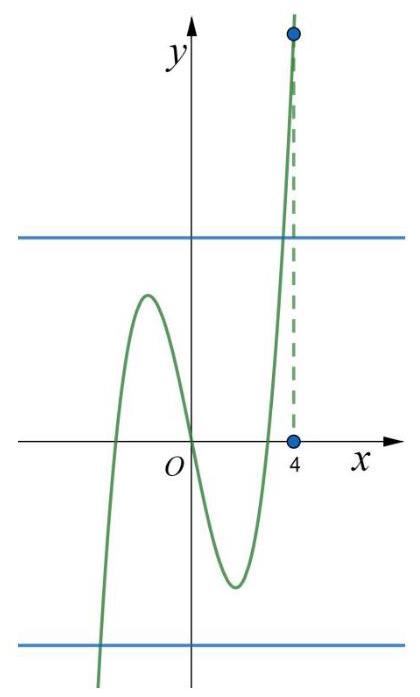
\includegraphics[max width=0.3\textwidth]{images/bo_d7fhnv491nqc73ercsbg_27_232_975_420_697_0.jpg}
\end{center}
\hspace*{3em} 

当 \(f\left( \sqrt{\frac{-m}{3}}\right)  = \frac{-m}{3}\sqrt{\frac{-m}{3}} + m\sqrt{\frac{-m}{3}} <  - {16} \Rightarrow  m <  - {12}\) 时,

如下图,

\begin{center}
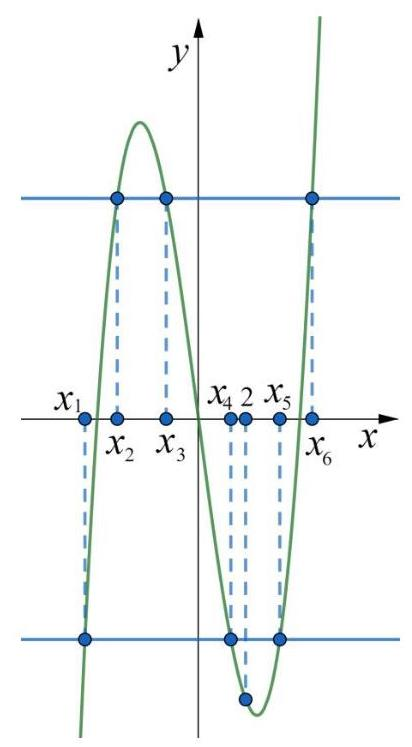
\includegraphics[max width=0.3\textwidth]{images/bo_d7fhnv491nqc73ercsbg_28_229_191_412_747_0.jpg}
\end{center}
\hspace*{3em} 

设 \({x}^{3} + {mx} + {16} = 0\) 的三个根分别为 \({x}_{1},{x}_{4},{x}_{5}\) ,

设 \({x}^{3} + {mx} - {16} = 0\) 的三个根分别为 \({x}_{2},{x}_{3},{x}_{6}\) ,

\(f\left( 2\right)  = 8 + {2m} <  - {16}\) ,故 \({x}_{4} < 2\) ,

由三次韦达定理可得 \({x}_{2} + {x}_{3} + {x}_{6} = 0,{x}_{1} + {x}_{4} + {x}_{5} = 0\) ,

\(T = {x}_{2} - {x}_{1} + {x}_{4} - {x}_{3} + {x}_{6} - {x}_{5} = 2\left( {{x}_{4} - {x}_{3}}\right)  = 4{x}_{4} < 8,\)

综上,当且仅当 \(m =  - {12}\) 时, \(T = 8\) .

6. (2025 高三二模普陀 12)设 \(a \in  \mathbf{R}\) ，函数 \(y = f\left( x\right)\) 的表达式为 \(f\left( x\right)  = \left\{  \begin{matrix} {\mathrm{e}}^{x} & x > 0 \\  \frac{1}{x + a} & x < 0 \end{matrix}\right.\) ， 若函数 \(g\left( x\right)  = f\left( x\right) f\left( {x + 1}\right)  - 1\) 恰有三个零点，则 \(a\) 的取值范围是\_\_\_\_\_.

【答案】 \(\left( {2,\mathrm{e}}\right)\)

【解析】设函数 \(g\left( x\right)\) 的零点为 \({x}_{0}\) ,

\({1}^{ \circ  }\) 当 \({x}_{0} > 0\) 时, \({x}_{0} + 1 > 1\) ,故 \(g\left( {x}_{0}\right)  = {\mathrm{e}}^{{x}_{0}} \cdot  {\mathrm{e}}^{{x}_{0} + 1} - 1 = 0\) ,解得 \({x}_{0} =  - \frac{1}{2}\) ,舍

2 \textdegree  当 \(- 1 < {x}_{0} < 0\) 时， \({x}_{0} + 1 > 0\) ，故 \(g\left( {x}_{0}\right)  = \frac{{\mathrm{e}}^{{x}_{0} + 1}}{{x}_{0} + a} - 1 = 0\) ，即 \(a = {\mathrm{e}}^{{x}_{0} + 1} - {x}_{0}\) ，

令 \(h\left( x\right)  = {\mathrm{e}}^{x + 1} - x\left( {-1 < x < 0}\right)\) ,则 \({h}^{\prime }\left( x\right)  = {\mathrm{e}}^{x + 1} - 1 > 0\) 在 \(- 1 < x < 0\) 上恒成立,

故 \(h\left( x\right)  = {\mathrm{e}}^{x + 1} - x\) 在区间 \(\left( {-1,0}\right)\) 上严格递增,且 \(h\left( x\right)  \in  \left( {2,\mathrm{e}}\right)\) ,

当 \(a \in  \left( {2,\mathrm{e}}\right)\) 时, \(g\left( x\right)\) 在 \(\left( {-1,0}\right)\) 上有 1 个零点,

\({3}^{ \circ  }\) 当 \({x}_{0} <  - 1\) 时, \({x}_{0} + 1 < 0\) ,故 \(g\left( {x}_{0}\right)  = \frac{1}{{x}_{0} + a} \cdot  \frac{1}{{x}_{0} + 1 + a} - 1 = 0\) ,

即 \({x}_{0}^{2} + \left( {{2a} + 1}\right) {x}_{0} + {a}^{2} + a - 1 = 0\) ,由于方程至多有两个根,

由 \({2}^{ \circ  }\) 可知, \(a\) 的取值范围为 \(\left( {2,\mathrm{e}}\right)\) 的子集,

令 \(p\left( x\right)  = {x}_{0}^{2} + \left( {{2a} + 1}\right) {x}_{0} + {a}^{2} + a - 1\) ,其中 \(\Delta  = {\left( 2a + 1\right) }^{2} - 4\left( {{a}^{2} + a - 1}\right)  = 5 > 0\) ,

\(p\left( {-1}\right)  = 1 - \left( {{2a} + 1}\right)  + {a}^{2} + a - 1 = {a}^{2} - a - 1 = {\left( a - \frac{1}{2}\right) }^{2} - \frac{5}{4},\)

当 \(a \in  \left( {2,\mathrm{e}}\right)\) 时, \(p\left( {-1}\right)  = {\left( a - \frac{1}{2}\right) }^{2} - \frac{5}{4} > {\left( 2 - \frac{1}{2}\right) }^{2} - \frac{5}{4} = 1\) ,

函数 \(p\left( x\right)  = {x}_{0}^{2} + \left( {{2a} + 1}\right) {x}_{0} + {a}^{2} + a - 1\) 图像的对称轴 \(x =  - a - \frac{1}{2} <  - \frac{5}{2}\) ,

故 \(p\left( x\right)  = {x}_{0}^{2} + \left( {{2a} + 1}\right) {x}_{0} + {a}^{2} + a - 1\) 在 \(x \in  \left( {-\infty , - 1}\right)\) 上有两个不相等的实数根,

综上,当 \(a \in  \left( {2,\mathrm{e}}\right)\) 时, \(g\left( x\right)\) 有三个零点.

7.(2025 高三二模静安 15)设 \(y = f\left( x\right)\) 是一个三次函数， \(y = {f}^{\prime }\left( x\right)\) 为其导函数.如图所示的是函数 \(y = x{f}^{\prime }\left( x\right)\) 的图像的一部分. 则 \(y = f\left( x\right)\) 的极大值与极小值分别为 ( )

A. \(f\left( 1\right)\) 与 \(f\left( {-1}\right)\) ; B. \(f\left( {-1}\right)\) 与 \(f\left( 1\right)\) ;

C. \(f\left( {-2}\right)\) 与 \(f\left( 2\right)\) ; D. \(f\left( 2\right)\) 与 \(f\left( {-2}\right)\) .

【答案】C

【解析】当 \(x \in  \left( {-\infty , - 2}\right)\) 时, \(x{f}^{\prime }\left( x\right)  < 0 \Rightarrow  {f}^{\prime }\left( x\right)  > 0\) ,单调递增,

当 \(x \in  \left( {-2,0}\right)\) 时, \(x{f}^{\prime }\left( x\right)  > 0 \Rightarrow  {f}^{\prime }\left( x\right)  < 0\) ,单调递减,

当 \(x \in  \left( {0,2}\right)\) 时, \(x{f}^{\prime }\left( x\right)  < 0 \Rightarrow  {f}^{\prime }\left( x\right)  < 0\) ,单调递减,

当 \(x \in  \left( {2, + \infty }\right)\) 时, \(x{f}^{\prime }\left( x\right)  > 0 \Rightarrow  {f}^{\prime }\left( x\right)  > 0\) ,单调递增,

则 \(x \in  \left( {-\infty , - 2}\right)\) 和 \(\left( {2, + \infty }\right) ,{f}^{\prime }\left( x\right)  > 0,f\left( x\right)\) 单调递增, \(x \in  \left( {-2,2}\right) ,{f}^{\prime }\left( x\right)  < 0,f\left( x\right)\) 单调递减,则在 \(x =  - 2\) 时取到极大值,在 \(x = 2\) 时取到极小值,故选 \(\mathrm{C}\) .

8.(2025 高三二模奉贤 15)函数 \(y = f\left( x\right)\) 的导函数为 \(y = g\left( x\right)\) ，若存在实数 \({x}_{0}\) ，使得 \(g\left( {x}_{0}\right) f\left( {-{x}_{0}}\right)  = 1\) 成立,则称函数 \(y = f\left( x\right)\) 具有 \({x}_{0}\) 性质,下列函数 \(y = f\left( x\right)\) 具有 \({x}_{0}\) 性质的函数是( )

A. \(y = {\mathrm{e}}^{-x}\) B. \(y = \sin x\)

C. \(y = {\mathrm{e}}^{x} + {\mathrm{e}}^{-x}\)

D. \(y = \frac{1}{2}\ln \left( {{x}^{2} + 1}\right)\)

【答案】C

【解析】对于 \(\mathrm{A},{y}^{\prime } =  - {e}^{-x}, - {e}^{-{x}_{0}} \cdot  {e}^{{x}_{0}} =  - 1 \neq  1\) ,则 \(\mathrm{A}\) 不具有;

对于 \(\mathrm{B},{y}^{\prime } = \cos x,\cos x \cdot  \left( {-\sin x}\right)  =  - \frac{1}{2}\sin {2x} \in  \left\lbrack  {-\frac{1}{2},\frac{1}{2}}\right\rbrack\) ,则 \(\mathrm{B}\) 不具有;

对于 \(\mathrm{C},{y}^{\prime } = {e}^{x} - {e}^{-x},\left( {{e}^{{x}_{0}} - {e}^{-{x}_{0}}}\right) \left( {{e}^{-{x}_{0}} + {e}^{{x}_{0}}}\right)  = {e}^{2{x}_{0}} - {e}^{-2{x}_{0}} = 1 \Rightarrow  {e}^{{x}_{0}} = \frac{1 + \sqrt{5}}{2}\) ,方程有解, 则具有 \({x}_{0}\) 性质;

对于 \(\mathrm{D},{y}^{\prime } = \frac{x}{{x}^{2} + 1},g\left( {x}_{0}\right) f\left( {-{x}_{0}}\right)  = 1 \Leftrightarrow  \frac{{x}_{0}}{{x}_{0}{}^{2} + 1}\ln \left( {{x}_{0}{}^{2} + 1}\right)  = 2\) 显然 \({x}_{0} \leq  0\) 上式无解,当 \({x}_{0} > 0\) 时, \(g\left( {x}_{0}\right) f\left( {-{x}_{0}}\right)  = 1 \Leftrightarrow  \ln \left( {{x}_{0}^{2} + 1}\right)  = 2\left( {{x}_{0} + \frac{1}{{x}_{0}}}\right)\) 设 \(h\left( {x}_{0}\right)  = \ln \left( {{x}_{0}^{2} + 1}\right)  - 2{x}_{0}\left( {{x}_{0} > 0}\right)\) ,则 \({h}^{\prime }\left( {x}_{0}\right)  = \frac{-2\left( {{x}_{0}^{2} - {x}_{0} + 1}\right) }{{x}_{0}{}^{2} + 1} < 0\) ,所以 \(h\left( {x}_{0}\right)  < h\left( 0\right)  = 0\) ,即 \(\ln \left( {{x}_{0}{}^{2} + 1}\right)  - 2{x}_{0} < 0\) ,所以 \(\ln \left( {{x}_{0}{}^{2} + 1}\right)  < 2{x}_{0} < 2\left( {{x}_{0} + \frac{1}{{x}_{0}}}\right)\) ,

所以 \(g\left( {x}_{0}\right) f\left( {-{x}_{0}}\right)  = 1\) 无解;

故选 C.

9.(2025 高三二模松江 16)定义在 \(\left( {0, + \infty }\right)\) 上的函数 \(y = f\left( x\right)\) 满足

\(f\left( {x + 1}\right)  = f\left( x\right)  - x\) ,当 \(0 < x \leq  1\) 时, \(f\left( x\right)  = \sqrt{x} - x + 1\) ,有以下两个命题:

 \circled{1}  当 \(n\) 为正整数时， \(f\left( n\right)  = \frac{-{n}^{2} + n + 2}{2}\) ；

 \circled{2} 若函数 \(y = f\left( x\right)\) 在区间 \((0,k\rbrack\) 内有 3 个极大值点,则 \(k\) 的取值范围是 \(\left\lbrack  {\frac{73}{36},3}\right)\) .

则以下选项正确的是 ( )

A.  \circled{1} 是真命题， \circled{2} 是假命题 B. 两个都是真命题

C.  \circled{1} 是假命题， \circled{2} 是真命题 D. 两个都是假命题

【答案】A

【解析】 \circled{1}  当 \(n \geq  1,n \in  \mathbf{N}\) 时, \(f\left( {n + 1}\right)  - f\left( n\right)  =  - n\)

\(f\left( n\right)  - f\left( {n - 1}\right)  =  - \left( {n - 1}\right) ,\;f\left( {n - 1}\right)  - f\left( {n - 2}\right)  =  - \left( {n - 2}\right) ,\ldots \ldots\)

\(f\left( 3\right)  - f\left( 2\right)  =  - 2,f\left( 2\right)  - f\left( 1\right)  =  - 1,f\left( 1\right)  = \sqrt{1} - 1 + 1 = 1,\)

则

\(f\left( n\right)  = \left\lbrack  {f\left( n\right)  - f\left( {n - 1}\right) }\right\rbrack   + \left\lbrack  {f\left( {n - 1}\right)  - f\left( {n - 2}\right) }\right\rbrack   + \cdots \left\lbrack  {f\left( 3\right)  - f\left( 2\right) }\right\rbrack   + \left\lbrack  {f\left( 2\right)  - f\left( 1\right) }\right\rbrack   + f\left( 1\right) \; =  - \left\lbrack  {\left( {n - 1}\right)  + \left( {n - 2}\right)  + \cdots  + 2 + 1}\right\rbrack   + 1 =  - \frac{\left( {n - 1}\right) \left( {n - 1 + 1}\right) }{2} + 1 \; = \frac{-{n}^{2} + n + 2}{2}\) ,所以 \circled{1} 正确;

 \circled{2}  当 \(x \in  (0,1\rbrack\) 时， \({f}^{\prime }\left( x\right)  = \frac{1}{2\sqrt{x}} - 1\) ，当 \(x \in  \left( {0,\frac{1}{4}}\right)\) 时， \({f}^{\prime }\left( x\right)  > 0\) ，当 \(x \in  \left( {\frac{1}{4},1}\right)\) 时， \({f}^{\prime }\left( x\right)  < 0\) ,所以 \(f\left( x\right)\) 在 \((0,1\rbrack\) 上有 1 个极大值点 \(x = \frac{1}{4}\) ;

当 \(x \in  (1,2\rbrack ,f\left( x\right)  = f\left( {x - 1}\right)  - \left( {x - 1}\right)  = \sqrt{x - 1} - {2x} + 3\) ,此时 \({f}^{\prime }\left( x\right)  = \frac{1}{2\sqrt{x - 1}} - 2\) , 当 \(x \in  \left( {1,\frac{17}{16}}\right)\) 时, \({f}^{\prime }\left( x\right)  > 0\) ,当 \(x \in  \left( {\frac{1}{16},2}\right)\) 时, \({f}^{\prime }\left( x\right)  < 0\) ,所以 \(f\left( x\right)\) 在 \((1,2\rbrack\) 上有 1 个极大值点 \(x = \frac{17}{16}\) ;

当 \(x \in  (2,3\rbrack\) 时, \(f\left( x\right)  = f\left( {x - 1}\right)  - \left( {x - 1}\right)  = \sqrt{x - 2} - 2\left( {x - 1}\right)  + 3 - \left( {x - 1}\right)  = \sqrt{x - 2} - {3x} + 6\) ,

此时 \({f}^{\prime }\left( x\right)  = \frac{1}{2\sqrt{x - 2}} - 3\) ,当 \(x \in  \left( {2,\frac{73}{36}}\right)\) 时, \({f}^{\prime }\left( x\right)  > 0\) ,当 \(x \in  \left( {\frac{73}{36},3}\right)\) 时, \({f}^{\prime }\left( x\right)  < 0\) ,

所以 \(f\left( x\right)\) 在 \(\left( {2,3}\right\rbrack\) 上有 1 个极大值点 \(x = \frac{73}{36}\) ;

当 \(x \in  (3,4\rbrack\) 时, \(f\left( x\right)  = f\left( {x - 1}\right)  - \left( {x - 1}\right)  = \sqrt{x - 3} - 3\left( {x - 1}\right)  + 6 - \left( {x - 1}\right)  = \sqrt{x - 3} - {4x} + {10}\) ,

此时 \({f}^{\prime }\left( x\right)  = \frac{1}{2\sqrt{x - 3}} - 4\) ,当 \(x \in  \left( {3,\frac{193}{64}}\right)\) 时, \({f}^{\prime }\left( x\right)  > 0\) ,当 \(x \in  \left( {\frac{193}{64},4}\right)\) 时, \({f}^{\prime }\left( x\right)  < 0\) , 所以 \(f\left( x\right)\) 在 \(\left( {3,4}\right\rbrack\) 上有 1 个极大值点 \(x = \frac{193}{64}\) ;

所以函数 \(y = f\left( x\right)\) 在区间 \((0,k\rbrack\) 内有 3 个极大值点,则 \(k\) 的取值范围是 \(\left\lbrack  {\frac{73}{36},\frac{193}{64}}\right)\) ,所以  \circled{2} 错误;

故选 A.

10.(2025 高三二模徐汇 16)已知函数 \(y = f\left( x\right)\) 的定义域和值域都为 \(\mathbf{R}\) ，且图像是一条连续不断的曲线,其导函数 \(y = {f}^{\prime }\left( x\right)\) 的值如下表:

\begin{center}
\adjustbox{max width=\textwidth}{
\begin{tabular}{|c|c|c|c|c|c|}
\hline
\(x\) & \(\left( {-\infty ,{x}_{1}}\right)\) & \({x}_{1}\) & \(\left( {{x}_{1},{x}_{2}}\right)\) & \({x}_{2}\) & \(\left( {{x}_{2}, + \infty }\right)\) \\
\cline{1-6}
\({f}^{\prime }\left( x\right)\) & + & 0 & - & 0 & + \\
\cline{1-6}
\hline
\end{tabular}
}
\end{center}

设 \(D \subseteq  \mathbf{R}\) ,若集合 \(\{ y \mid  y = f\left( x\right) ,x \in  D\}  = \{ a,b,c\}\) ,其中 \(a,b,c\) 为常数,则符合要求的集合 \(D\) 的个数不可能是( )

A. 3 B. 27 C. 63 D. 343

【答案】B

【解析】由题意可得,若对应的 \(y = t\) 的 \(x\) 取值的情况可以有 1 个,2 个或 3 个,且对应 2 个根的情况的时候, \(t\) 的取值只要 2 个,

若 \(y = a,y = b,y = c\) 对应的根的个数为1,1,2,则符合要求的集合的个数为 \(1 \times  1 \times  \left( {{2}^{2} - 1}\right)  = 3\) , A 有可能;

若 \(y = a,y = b,y = c\) 对应的根的个数为2,2,3,则符合要求的集合的个数为 \(\left( {{2}^{2} - 1}\right)  \times  \left( {{2}^{2} - 1}\right)  \times  \left( {{2}^{3} - 1}\right)  = {63},\mathrm{C}\) 有可能;

若 \(y = a,y = b,y = c\) 对应的根的个数为3,3,2,则符合要求的集合的个数为 \(\left( {{2}^{3} - 1}\right)  \times  \left( {{2}^{3} - 1}\right)  \times  \left( {{2}^{3} - 1}\right)  = {343},\mathrm{D}\) 有可能;

故选 B.

11. (2025 高三二模松江 21)已知 \(f\left( x\right)  = \ln \left( {x - 1}\right)  + \frac{2a}{x} - \frac{4}{3},a \in  \mathrm{R}\) .

(1)若 \(x = 4\) 是函数 \(y = f\left( x\right)\) 的一个极值点，求曲线 \(y = f\left( x\right)\) 在点 \(P\left( {4,f\left( 4\right) }\right)\) 处的切线方程;

(2)讨论函数 \(y = f\left( x\right)\) 的单调性;

(3)已知实数 \(a = 0\) ，若点 \(A\left( {{x}_{1},{y}_{1}}\right)\) 、 \(B\left( {{x}_{2},{y}_{2}}\right) \left( {{x}_{1} < {x}_{2}}\right)\) 是曲线 \(y = f\left( x\right)\) 上两点，直线 \({AB}\) 的斜率为 \(k\) ,求证: \({x}_{1} < \frac{1 + k}{k} < {x}_{2}\) .

【答案】(1) \(y = \ln 3\) ；(2) 当 \(a \leq  2\) 时， \(f\left( x\right)\) 在 \(\left( {1, + \infty }\right)\) 上单调递增；

当 \(a > 2\) 时， \(f\left( x\right)\) 在 \(\left( {1,a - \sqrt{{a}^{2} - {2a}}}\right)\) 和 \(\left( {a + \sqrt{{a}^{2} - {2a}}, + \infty }\right)\) 上单调递增，在

\(\left( {a - \sqrt{{a}^{2} - {2a}},a + \sqrt{{a}^{2} - {2a}}}\right)\) 上单调递减; (3) 证明见解析

【解析】(1) \(f\left( x\right)\) 的定义域为 \(\left( {1, + \infty }\right)\) ,

由 \(f\left( x\right)  = \ln \left( {x - 1}\right)  + \frac{2a}{x} - \frac{4}{3}\) ,得 \({f}^{\prime }\left( x\right)  = \frac{1}{x - 1} - \frac{2a}{{x}^{2}}\) ,

因为 \(x = 4\) 是函数 \(y = f\left( x\right)\) 的一个极值点,

所以 \({f}^{\prime }\left( 4\right)  = \frac{1}{4 - 1} - \frac{2a}{{4}^{2}} = 0\) ,即 \(\frac{1}{3} - \frac{a}{8} = 0\) ,解得 \(a = \frac{8}{3}\) , ...2 分

则 \(f\left( x\right)  = \ln \left( {x - 1}\right)  + \frac{16}{3x} - \frac{4}{3},{f}^{\prime }\left( x\right)  = \frac{1}{x - 1} - \frac{16}{3{x}^{2}} = \frac{\left( {x - 4}\right) \left( {{3x} - 4}\right) }{3{x}^{2}\left( {x - 1}\right) }\) ,

则 \({f}^{\prime }\left( x\right)  > 0\) 得 \(1 < x < \frac{4}{3}\) 或 \(x > 4;{f}^{\prime }\left( x\right)  < 0\) 得 \(\frac{4}{3} < x < 4\) ,

则 \(f\left( x\right)\) 在 \(\left( {1,\frac{4}{3}}\right)\) 和 \(\left( {4, + \infty }\right)\) 上单调递增,在 \(\left( {\frac{4}{3},4}\right)\) 上单调递减,

则 \(x = 4\) 是 \(f\left( x\right)\) 的极小值点，

又 \(f\left( 4\right)  = \ln 3 + \frac{4}{3} - \frac{4}{3} = \ln 3,{f}^{\prime }\left( 4\right)  = 0\) ,

则切线方程为 \(y - \ln 3 = 0\left( {x - 4}\right)\) ,整理得 \(y = \ln 3\) . 2 分

(2) \(f\left( x\right)\) 的定义域为 \(\left( {1, + \infty }\right) ,{f}^{\prime }\left( x\right)  = \frac{1}{x - 1} - \frac{2a}{{x}^{2}} = \frac{{x}^{2} - {2ax} + {2a}}{{x}^{2}\left( {x - 1}\right) }\) ，

令 \(g\left( x\right)  = {x}^{2} - {2ax} + {2a}\) ,其对称轴为 \(x = a,\Delta  = 4{a}^{2} - {8a} = {4a}\left( {a - 2}\right)\) ,

 \circled{1}  当 \(\Delta  \leq  0\) ,即 \(0 \leq  a \leq  2\) 时， \(g\left( x\right)  \geq  0,{f}^{\prime }\left( x\right)  \geq  0\) ，则 \(f\left( x\right)\) 在 \(\left( {1, + \infty }\right)\) 上单调递增；

 \circled{2} 当 \(\Delta  > 0\) ,即 \(a < 0\) 或 \(a > 2\) 时,

(i) 当 \(a > 2\) 时, \(g\left( x\right)  = 0\) 的两根为 \({x}_{1} = a - \sqrt{{a}^{2} - {2a}},{x}_{2} = a + \sqrt{{a}^{2} - {2a}}\) ,

且 \(1 < {x}_{1} < {x}_{2}\) ,

则当 \(1 < x < {x}_{1}\) 或 \(x > {x}_{2}\) 时, \(g\left( x\right)  > 0,{f}^{\prime }\left( x\right)  > 0\) ;

当 \({x}_{1} < x < {x}_{2}\) 时, \(g\left( x\right)  < 0,{f}^{\prime }\left( x\right)  < 0\) .

(ii) 当 \(a < 0\) 时, \(g\left( x\right)\) 的对称轴 \(x = a < 0\) ,且 \(g\left( 1\right)  = 1\) ,

则 \(g\left( x\right)  > 0\) 在 \(\left( {1, + \infty }\right)\) 上恒成立,即 \({f}^{\prime }\left( x\right)  > 0\) 在 \(\left( {1, + \infty }\right)\) 上恒成立.

综上,当 \(a \leq  2\) 时, \(f\left( x\right)\) 在 \(\left( {1, + \infty }\right)\) 上单调递增;

当 \(a > 2\) 时, \(f\left( x\right)\) 在 \(\left( {1,a - \sqrt{{a}^{2} - {2a}}}\right)\) 和 \(\left( {a + \sqrt{{a}^{2} - {2a}}, + \infty }\right)\) 上单调递增,在 \(\left( {a - \sqrt{{a}^{2} - {2a}},a + \sqrt{{a}^{2} - {2a}}}\right)\) 上单调递减. ...4 分

(3)已知 \(a = 0\) ，则 \(f\left( x\right)  = \ln \left( {x - 1}\right)  - \frac{4}{3}\) ，

则 \(k = \frac{f\left( {x}_{2}\right)  - f\left( {x}_{1}\right) }{{x}_{2} - {x}_{1}} = \frac{\ln \left( {{x}_{2} - 1}\right)  - \ln \left( {{x}_{1} - 1}\right) }{{x}_{2} - {x}_{1}}\) ,

则 \(\frac{1 + k}{k} = \frac{1}{k} + 1 = \frac{{x}_{2} - {x}_{1}}{\ln \left( {{x}_{2} - 1}\right)  - \ln \left( {{x}_{1} - 1}\right) } + 1\) ,

要证 \({x}_{1} < \frac{1 + k}{k} < {x}_{2}\) ,即证 \({x}_{1} < \frac{{x}_{2} - {x}_{1}}{\ln \left( {{x}_{2} - 1}\right)  - \ln \left( {{x}_{1} - 1}\right) } + 1 < {x}_{2}\) , ...2 分

即证 \({x}_{1} - 1 < \frac{{x}_{2} - {x}_{1}}{\ln \frac{{x}_{2} - 1}{{x}_{1} - 1}} < {x}_{2} - 1\) , ...2 分

令 \(t = \frac{{x}_{2} - 1}{{x}_{1} - 1}\left( {t > 1}\right)\) ,则只需证 \(1 < \frac{t - 1}{\ln t} < t\) ,

先证 \(\frac{t - 1}{\ln t} > 1\left( {t > 1}\right)\) ,即证 \(t - 1 > \ln t\) ,

令 \(h\left( t\right)  = t - 1 - \ln t\left( {t > 1}\right)\) ,则 \({h}^{\prime }\left( t\right)  = 1 - \frac{1}{t} = \frac{t - 1}{t} > 0\) ,

所以 \(h\left( t\right)\) 在 \(\left( {1, + \infty }\right)\) 上单调递增,则 \(h\left( t\right)  > h\left( 1\right)  = 0\) ,即 \(t - 1 > \ln t\) ; ..2 分

再证 \(\frac{t - 1}{\ln t} < t\left( {t > 1}\right)\) ,即证 \(t - 1 < t\ln t\) ,

令 \(m\left( t\right)  = t\ln t - \left( {t - 1}\right) \left( {t > 1}\right)\) ,则 \({m}^{\prime }\left( t\right)  = \ln t + 1 - 1 = \ln t > 0\) ,

所以 \(m\left( t\right)\) 在 \(\left( {1, + \infty }\right)\) 上单调递增,则 \(m\left( t\right)  > m\left( 1\right)  = 0\) ,即 \(t - 1 < t\ln t\) . ..2 分综上, \({x}_{1} < \frac{1 + k}{k} < {x}_{2}\) 得证.

12.(2025 高三二模长宁 21)已知函数 \(y = f\left( x\right)\) 的定义域 \(\mathbf{D} \subseteq  \mathbf{R}\) ，对任意实数 \(a\) ，定义集合 \({Q}_{f}\left( a\right)  = \left\{  {x \mid  f\left( x\right)  \leq  a,x \in  \mathbf{D}}\right\}\) .

(1)已知 \(f\left( x\right)  = \frac{1 + x}{1 - x}\) ，求 \({Q}_{f}\left( 2\right)\) ；

(2)已知 \(f\left( x\right)  = {e}^{x} - {ax}\) ，若集合 \({Q}_{f}\left( a\right)\) 只有一个元素，求 \(a\) 的值；

(3)已知 \(f\left( x\right)  =  - \frac{a}{4}{x}^{2} + \frac{a + 2}{2}x - \ln x + \frac{1}{2}\) ，其中 \(a \in  \mathbf{R}\) 且 \(a > 0\) ，求证:集合 \({Q}_{f}\left( a\right)\) 是一个区间.

【答案】(1) \({Q}_{f}\left( 2\right)  = \left\{  {x \mid  x > 1\text{ 或 }x \leq  \frac{1}{3}}\right\}  ;\left( 2\right) a = 1;\left( 3\right)\) 证明见解析

【解析】(1) 由题意得: \(\frac{1 + x}{1 - x} \leq  2\) , .2 分

解得: \(x > 1\) 或 \(x \leq  \frac{1}{3}\) ,即 \({Q}_{f}\left( 2\right)  = \left\{  {x \mid  x > 1\text{ 或 }x \leq  \frac{1}{3}}\right\}\) , .2 分

( 2 )集合 \({Q}_{f}\left( a\right)\) 只有一个元素，则满足 \({e}^{x} - {ax} - a \leq  0\) 的 \(x\) 有且只有 1 个，

令 \(g\left( x\right)  = {e}^{x} - {ax} - a,{g}^{\prime }\left( x\right)  = {e}^{x} - a\)

若 \(a < 0\) ,则 \({g}^{\prime }\left( x\right)  = {e}^{x} - a > 0\) ,函数 \(y = g\left( x\right)\) 严格增,

当 \(x\) 趋于 \(- \infty\) 时, \(g\left( x\right)  = {e}^{x} - {ax} - a\) 趋于 \(- \infty\) ,

所以满足 \({e}^{x} - {ax} - a \leq  0\) 的 \(x\) 不止 1 个,舍; .2 分

若 \(a = 0\) ,由于 \({e}^{x} > 0\) ,所以 \({e}^{x} - {ax} - a \leq  0\) 的解集为空集,舍; 1 分

若 \(a > 0\) ,则函数 \(y = g\left( x\right)\) 在 \(\left( {-\infty ,\ln a}\right)\) 上严格增,在 \(\left( {\ln a, - \infty }\right)\) 上严格减

即有 \(g\left( x\right)  \geq  g\left( {\ln a}\right)  =  - a\ln a\) ,

由于满足 \({e}^{x} - {ax} - a \leq  0\) 的 \(x\) 有且只有 1 个,

所以 \(- a\ln a = 0,a = 1\) ; .3 分

(3) \({f}^{\prime }\left( x\right)  =  - \frac{a}{2}x + \frac{a + 2}{2} - \frac{1}{x} =  - \frac{\left( {{ax} - 2}\right) \left( {x - 1}\right) }{2x}\) , .2 分

若 \(a = 2\) ,则 \({f}^{\prime }\left( x\right)  \leq  0\) ,且仅当 \(x = 1\) 时, \({f}^{\prime }\left( x\right)  = 0\) ,所以函数 \(y = f\left( x\right)\) 在 \(\left( {0,1}\right)\) 上严格减, 当 \(x\) 趋于 0 时, \(y = f\left( x\right)\) 趋于 \(+ \infty\) ,当 \(x\) 趋于 \(+ \infty\) 时, \(y = f\left( x\right)\) 趋于 \(- \infty\) ,

又 \(f\left( 1\right)  = 2\) ,所以 \({Q}_{f}\left( a\right)  = \lbrack 1, + \infty )\) 为区间, .2 分

若 \(0 < a < 2\) ,则函数 \(y = f\left( x\right)\) 在 \(\left( {0,1}\right)\) 上严格减,在 \(\left( {1,\frac{2}{a}}\right)\) 上严格增,在 \(\left( {\frac{2}{a}, + \infty }\right)\) 上严格减, 且当 \(x\) 趋于 0 时, \(y = f\left( x\right)\) 趋于 \(+ \infty\) ,当 \(x\) 趋于 \(+ \infty\) 时, \(y = f\left( x\right)\) 趋于 \(- \infty\) ,

即函数 \(y = f\left( x\right)\) 在 \(x = 1\) 处取得极小值,在 \(x = \frac{2}{a}\) 处取得极大值, .2 分因为 \(0 < a < 2\) ,所以 \(a < \frac{a}{4} + \frac{3}{2}\) ,即 \(a < f\left( 1\right)\)

由于 \(f\left( \frac{2}{a}\right)  > f\left( 1\right)\) ,且 \(x\) 趋于 \(+ \infty\) 时, \(y = f\left( x\right)\) 趋于 \(- \infty\) ,

所以由零点存在定理,知存在 \({x}_{1} \in  \left( {\frac{2}{a}, + \infty }\right)\) ,使得 \(f\left( {x}_{1}\right)  = f\left( 1\right)\)

又由于 \(f\left( {x}_{1}\right)  > a\) ,所以存在 \({x}_{2} \in  \left( {{x}_{1}, + \infty }\right)\) ,使得 \(f\left( {x}_{2}\right)  = a\)

则 \({Q}_{f}\left( a\right)  = \left\lbrack  {{x}_{2}, + \infty }\right)\) 为区间, .1 分

同理,若 \(a > 2\) ,函数 \(y = f\left( x\right)\) 在 \(x = \frac{2}{a}\) 处取得极小值,在 \(x = 1\) 处取得极大值,

因为 \(a > 2\) ,所以 \(a > \frac{a}{4} + \frac{3}{2}\) ,即 \(a > f\left( 1\right)\)

由于 \(f\left( \frac{2}{a}\right)  < f\left( 1\right)\) ,且 \(x\) 趋于 0 时, \(y = f\left( x\right)\) 趋于 \(+ \infty\) ,

所以存在 \({x}_{3} \in  \left( {0,\frac{2}{a}}\right)\) ,使得 \(f\left( {x}_{3}\right)  = f\left( 1\right)\)

又由于 \(a > f\left( {x}_{3}\right)\) ,所以存在 \({x}_{4} \in  \left( {0,{x}_{3}}\right)\) ,使得 \(f\left( {x}_{4}\right)  = a\)

则 \({Q}_{f}\left( a\right)  = \left\lbrack  {{x}_{4}, + \infty }\right)\) 为区间 1 分

13.(2025 高三二模静安 21)若存在实数常数 \(k\) ， \(m\) ，对任意 \(x \in  \mathbf{D}\) ，不等式

\(f\left( x\right)  \geq  {kx} + m \geq  g\left( x\right)\) 恒成立,则称直线 \(y = {kx} + m\) 是函数 \(y = f\left( x\right)\) 和函数 \(y = g\left( x\right)\) 在 \(\mathbf{D}\) 上的分界线.

(1)请写出函数 \(y = \frac{1}{2}{x}^{2}\) 和函数 \(y = \ln x\) 在 \(\left( {0, + \infty }\right)\) 上的一条斜率为 1 的分界线; (不必证

明)

(2)求证:函数 \(y = x + \frac{1}{x}\) 和函数 \(y = 2 - \frac{1}{x}\) 在 \(\left( {0, + \infty }\right)\) 上过坐标原点的分界线有且只有一条;

(3)试探究函数 \(y = {\mathrm{e}}^{x}\left( {x + 1}\right)\) ( \(\mathrm{e}\) 为自然对数的底数) 和函数 \(y =  - {x}^{2} + {2x} + 1\) 在 \(\mathbf{R}\) 上是否存在分界线.若存在, 求出分界线方程; 若不存在, 请说明理由.

【答案】(1) \(y = x + b\left( {b \in  \left\lbrack  {-\frac{1}{2}, - 1}\right\rbrack  }\right)\) ; (2) 证明见解析; (3) 存在, 方程为 \(y = {2x} + 1\) .

【解析】(1) \(y = x + b\left( {b \in  \left\lbrack  {-\frac{1}{2}, - 1}\right\rbrack  }\right)\) . (4 分)

(2)当 \(x \in  \left( {0, + \infty }\right)\) 时， \(x + \frac{1}{x} > x\) ； \(x \geq  2 - \frac{1}{x}\) (因为 \(x + \frac{1}{x} \geq  2\) ).

所以, \(y = x\) 是函数 \(y = x + \frac{1}{x}\) 和函数 \(y = 2 - \frac{1}{x}\) 在 \(\left( {0, + \infty }\right)\) 上过坐标原点的分界线. (1 分) 设 \(y = {kx}\) 是函数 \(y = x + \frac{1}{x}\) 和函数 \(y = 2 - \frac{1}{x}\) 在 \(\left( {0, + \infty }\right)\) 上过坐标原点的分界线.

当 \(x \in  \left( {0, + \infty }\right)\) 时,若 \(k > 1\) ,则不等式 \({kx} > x + \frac{1}{x}\) 有解为 \(x > \frac{1}{\sqrt{k - 1}}\) ,得 \(k \leq  1\) ; (2

若 \(k < 1\) ,则不等式 \({kx} < 2 - \frac{1}{x}\) 的解集为 \(\left( {\frac{-k - \sqrt{4 - {4k}}}{2k},\frac{-k + \sqrt{4 - {4k}}}{2k}}\right)\) ,得 \(k \geq  1.\) (2 分) 故， \(k = 1.\) (1 分)

(3)若存在,则 \({\mathrm{e}}^{x}\left( {x + 1}\right)  \geq  {kx} + m \geq   - {x}^{2} + {2x} + 1\) 恒成立. 令 \(x = 0\) ,则 \(1 \geq  m \geq  1\) ,所以 \(m = 1\) .

因此, \({kx} + m \geq   - {x}^{2} + {2x} + 1\) 恒成立,即 \({x}^{2} + \left( {k - 2}\right) x \geq  0\) 恒成立,由 \(\Delta  \leq  0\) 得, \(k = 2\) . (1 分)

现在只要判断 \({\mathrm{e}}^{x}\left( {x + 1}\right)  \geq  {2x} + 1\) 是否恒成立. 设 \(\varphi \left( x\right)  = {\mathrm{e}}^{x}\left( {x + 1}\right)  - \left( {{2x} + 1}\right)\) ,

则 \({\varphi }^{\prime }\left( x\right)  = {\mathrm{e}}^{x}\left( {x + 2}\right)  - 2\) ， (1 分)

当 \(x > 0\) 时， \({\mathrm{e}}^{x} > 1,x + 2 > 2,{\varphi }^{\prime }\left( x\right)  > 0\) ，

当 \(x < 0\) 时， \({\mathrm{e}}^{x}\left( {x + 2}\right)  < 2{\mathrm{e}}^{x} < 2,{\varphi }^{\prime }\left( x\right)  < 0\) ，

所以 \(\varphi \left( x\right)  \geq  \varphi \left( 0\right)  = 0\) ,即 \({\mathrm{e}}^{x}\left( {x + 1}\right)  \geq  {2x} + 1\) 恒成立. (4 分)

所以,函数 \(y = {\mathrm{e}}^{x}\left( {x + 1}\right)\) 和函数 \(y =  - {x}^{2} + {2x} + 1\) 在 \(\mathbf{R}\) 上存在分界线,

其方程为 \(y = {2x} + 1\) . (1 分)

14.(2025 高三二模杨浦 21)已知函数 \(y = f\left( x\right)\) 的导函数为 \(y = {f}^{\prime }\left( x\right)\) ，若函数 \(y = f\left( x\right)\) 的定义域为 \(\mathbf{R}\) ,且不等式 \(f\left( x\right)  > {f}^{\prime }\left( x\right)\) 对任意 \(x \in  \mathbf{R}\) 成立,则称函数 \(y = f\left( x\right)\) 是 “超导函数”.

(1)判断 \(f\left( x\right)  = {\mathrm{e}}^{x} + 1\) 是否为“超导函数”，并说明理由;

(2)若函数 \(y = g\left( x\right)\) 与 \(y = h\left( x\right)\) 都是“超导函数”，且对任意 \(x \in  \mathbf{R}\) ，都有 \({h}^{\prime }\left( x\right)  > 0\) 、 \({g}^{\prime }\left( x\right)  < 0\) ， 记 \(F\left( x\right)  = g\left( x\right) h\left( x\right)\) ,求证: 函数 \(y = F\left( x\right)\) 是 “超导函数”;

(3) 已知函数 \(y = \varphi \left( x\right)\) 是 “超导函数” 且 \(\varphi \left( 1\right)  = \mathrm{e}\) ,若有且仅有一个实数 \(t\) 满足 \(\varphi \left( {\ln t + 1 - {at}}\right)  = {\mathrm{e}}^{\ln t + 1 - {at}}\) ,求 \(a\) 的取值范围.

【答案】(1) \(y = f\left( x\right)\) 是“超导函数”; (2) 证明见解析; (3) \(a \in  ( - \infty ,0\rbrack  \cup  \left\{  \frac{1}{e}\right\}\)

【解析】(1) 是,理由如下: \(f\left( x\right)  = {\mathrm{e}}^{x} + 1\) ,则 \({f}^{\prime }\left( x\right)  = {\mathrm{e}}^{x}\) , .2 满足 \(f\left( x\right)  > {f}^{\prime }\left( x\right)\) 对任意 \(x \in  \mathbf{R}\) 成立,故函数 \(y = f\left( x\right)\) 是 “超导函数” .4

(2)由 \({F}^{\prime }\left( x\right)  = {g}^{\prime }\left( x\right) h\left( x\right)  + g\left( x\right) {h}^{\prime }\left( x\right)\) ，可得 .6

\(F\left( x\right)  - {F}^{\prime }\left( x\right)  = g\left( x\right) h\left( x\right)  - {g}^{\prime }\left( x\right) h\left( x\right)  - g\left( x\right) {h}^{\prime }\left( x\right)  = \left\lbrack  {g\left( x\right)  - {g}^{\prime }\left( x\right) }\right\rbrack  \left\lbrack  {h\left( x\right)  - {h}^{\prime }\left( x\right) }\right\rbrack   - {g}^{\prime }\left( x\right) {h}^{\prime }\left( x\right)\) .8

因为函数 \(y = g\left( x\right)\) 与 \(y = h\left( x\right)\) 都是 “超导函数”,

所以不等式 \(g\left( x\right)  > {g}^{\prime }\left( x\right)\) 与 \(h\left( x\right)  > {h}^{\prime }\left( x\right)\) 对任意 \(x \in  \mathbf{R}\) 成立,

即 \(g\left( x\right)  - {g}^{\prime }\left( x\right)  > 0,h\left( x\right)  - {h}^{\prime }\left( x\right)  > 0\) ,则 \(\left\lbrack  {g\left( x\right)  - {g}^{\prime }\left( x\right) }\right\rbrack  \left\lbrack  {h\left( x\right)  - {h}^{\prime }\left( x\right) }\right\rbrack   > 0\)

而 \({g}^{\prime }\left( x\right) {h}^{\prime }\left( x\right)  < 0\) ,因此可得 \(F\left( x\right)  - {F}^{\prime }\left( x\right)  > 0\) 对任意 \(x \in  \mathbf{R}\) 成立,

所以函数 \(y = F\left( x\right)\) 是“超导函数”. .10

(3)因为 \(\varphi \left( 1\right)  = \mathrm{e}\) ，所以 \(\varphi \left( {\ln t + 1 - {at}}\right)  = {\mathrm{e}}^{\ln t + 1 - {at}}\) 可化为 \(\frac{\varphi \left( {\ln t + 1 - {at}}\right) }{{\mathrm{e}}^{\ln t + 1 - {at}}} = \frac{\varphi \left( 1\right) }{{\mathrm{e}}^{1}}\) .

记 \(G\left( x\right)  = \frac{\varphi \left( x\right) }{{\mathrm{e}}^{x}}\) ,则原等式即为 \(G\left( {\ln t + 1 - {at}}\right)  = G\left( 1\right)\) , .12

由 \(y = \varphi \left( x\right)\) 是 “超导函数” 得 \(\varphi \left( x\right)  > {\varphi }^{\prime }\left( x\right)\) 对任意 \(x \in  \mathbf{R}\) 成立,

则 \({G}^{\prime }\left( x\right)  = \frac{{\varphi }^{\prime }\left( x\right)  - \varphi \left( x\right) }{{\mathrm{e}}^{x}} < 0\) 在 \(x \in  \mathbf{R}\) 恒成立,可知 \(y = G\left( x\right)\) 在 \(\mathbf{R}\) 上是严格减函数,

\(G\left( {\ln t + 1 - {at}}\right)  = G\left( 1\right)\) 等价于 \(\ln t + 1 - {at} = 1\) ,即有且仅有一个实数 \(t\) 满足 \(\ln t = {at}\) .14

令 \(H\left( x\right)  = \ln x - {ax}\) ,则 \({H}^{\prime }\left( x\right)  = \frac{1}{x} - a\)

i. 若 \(a = 0\) ,则 \(H\left( x\right)  = \ln x\) 只有一个零点;

ii. 若 \(a < 0\) ,

由 \(H\left( 1\right)  =  - a > 0\) ,且 \(H\left( {e}^{a}\right)  = a - a{e}^{a} = a\left( {1 - {e}^{a}}\right)  < 0\) ,可知存在 \({x}_{0} \in  \left( {{e}^{a},1}\right)\) 使得 \(H\left( {x}_{0}\right)  = 0\) .

(注: 此处 \(x\) 的取值不唯一)

由 \({H}^{\prime }\left( x\right)  > 0\) ,可知 \(H\left( x\right)\) 在 \(\left( {0, + \infty }\right)\) 上是严格增函数,则 \(H\left( x\right)\) 有且仅有一个零点.

iii. 若 \(a > 0\) ,令 \({H}^{\prime }\left( x\right)  = 0\) 解得 \(x = \frac{1}{a}\) ,

由 \(x \in  \left( {0,\frac{1}{a}}\right)\) 时, \({H}^{\prime }\left( x\right)  > 0,H\left( x\right)\) 在 \(\left( {0,\frac{1}{a}}\right)\) 上是严格增函数,

且 \(x \in  \left( {\frac{1}{a}, + \infty }\right)\) 时, \({H}^{\prime }\left( x\right)  < 0,H\left( x\right)\) 在 \(\left( {\frac{1}{a}, + \infty }\right)\) 上是严格减函数,

则 \(x = \frac{1}{a}\) 时, \(H\left( x\right)\) 取到最大值 \(H\left( \frac{1}{a}\right)  = \ln \frac{1}{a} - 1\) .

当 \(a > \frac{1}{e}\) 时, \(H\left( \frac{1}{a}\right)  = \ln \frac{1}{a} - 1 < 0,H\left( x\right)\) 无零点;

当 \(a = \frac{1}{e}\) 时, \(H\left( \frac{1}{a}\right)  = \ln \frac{1}{a} - 1 = 0\) ,由 \(H\left( x\right)\) 的单调性可知, \(H\left( x\right)\) 有且仅有一个零点;

当 \(0 < a < \frac{1}{e}\) 时， \(H\left( \frac{1}{a}\right)  = \ln \frac{1}{a} - 1 > 0\) ，

由 \(H\left( 1\right)  =  - a < 0\) 可知,存在 \({x}_{1} \in  \left( {1,\frac{1}{a}}\right)\) 使得 \(H\left( {x}_{1}\right)  = 0\) ; (注: 此处 \(x\) 的取值不唯一)

由 \(H\left( {\frac{1}{a} \cdot  {e}^{\frac{1}{a}}}\right)  = \ln \frac{1}{a} + \frac{1}{a} - {e}^{\frac{1}{a}}\) ,令 \(t = \frac{1}{a} \in  \left( {e, + \infty }\right)\) ,得 \(y = \ln t + t - {e}^{t},{y}^{\prime } = \frac{1}{t} + 1 - {e}^{t} < 0\) ,

则 \(y\) 在 \(t \in  \left( {e, + \infty }\right)\) 上是严格减函数,故 \(y < \ln e + e - {e}^{e} < 0\) ,则 \(H\left( {\frac{1}{a} \cdot  {e}^{\frac{1}{a}}}\right)  = \ln \frac{1}{a} + \frac{1}{a} - {e}^{\frac{1}{a}} < 0\) ,

可知存在 \({x}_{2} \in  \left( {\frac{1}{a},\frac{1}{a} \cdot  {e}^{\frac{1}{a}}}\right)\) 使得 \(H\left( {x}_{2}\right)  = 0\) . (注: 此处 \(x\) 的取值不唯一) .17

综上, \(a \in  ( - \infty ,0\rbrack  \cup  \left\{  \frac{1}{e}\right\}\) .18

另解:

记 \(m\left( x\right)  = \ln x\text{ 、 }n\left( x\right)  = {ax}\) ,则两个函数的图像有且仅有一个公共点

过原点作 \(m\left( x\right)  = \ln x\) 图像的切线,设切点为 \(\left( {{x}_{0},m\left( {x}_{0}\right) }\right)\) ,

则 \(\frac{m\left( {x}_{0}\right)  - 0}{{x}_{0} - 0} = {m}^{\prime }\left( {x}_{0}\right)\) ,即 \(\frac{\ln {x}_{0}}{{x}_{0}} = \frac{1}{{x}_{0}}\) ,解得 \({x}_{0} = e\) ,此时切线斜率为 \(\frac{1}{e}\) ,

结合 \(m\left( x\right)  = \ln x\) 与 \(n\left( x\right)  = {ax}\) 的图像可知,

当 \(a > \frac{1}{e}\) 时, \(m\left( x\right)  = \ln x\) 与 \(n\left( x\right)  = {ax}\) 的图像无公共点;

当 \(a = \frac{1}{e}\) 时, \(m\left( x\right)  = \ln x\) 与 \(n\left( x\right)  = {ax}\) 的图像相切;

当 \(0 < a < \frac{1}{e}\) 时, \(m\left( x\right)  = \ln x\) 与 \(n\left( x\right)  = {ax}\) 的图像有两个交点;

当 \(a \leq  0\) 时, \(m\left( x\right)  = \ln x\) 与 \(n\left( x\right)  = {ax}\) 的图像有一个交点. .17

综上, \(a \in  ( - \infty ,0\rbrack  \cup  \left\{  \frac{1}{e}\right\}\) .18

15.(2025 高三二模奉贤 21)函数 \(y = f\left( x\right)\) ，其中 \(f\left( x\right)  = {x}^{3} - {x}^{2} + \frac{1}{2}x + \frac{1}{4}\) ，定义域是一切实数.

(1)计算 \(\mathop{\lim }\limits_{{h \rightarrow  0}}\frac{f\left( {2 + h}\right)  - f\left( 2\right) }{h}\) 的值并指出其几何意义;

(2)当 \(x \in  \left( {0,\frac{1}{2}}\right)\) 时,方程 \(f\left( x\right)  = a + x\) 只有一个解,求实数 \(a\) 的取值范围;

(3)设 \({x}_{1} = 0,{x}_{n + 1} = f\left( {x}_{n}\right) ,{y}_{1} = \frac{1}{2},{y}_{n + 1} = f\left( {y}_{n}\right) ,n \geq  1,n \in  \mathbf{N},{b}_{n} = {y}_{n} - {x}_{n}\) . 求证: \(\mathop{\sum }\limits_{{i = 1}}^{n}{b}_{n} \in  \left( {0,1}\right)\) .

【答案】(1) \(\frac{17}{2}\) ，几何意义是函数在点 \(\left( {2,\frac{21}{4}}\right)\) 处切线的斜率是 \(\frac{17}{2}\) ；(2) \(\left( {-\frac{1}{8},\frac{1}{4}}\right)\) ；(3)

证明见解析

【解析】(1) \(f\left( 2\right)  = \frac{21}{4}\) , 1 分

原式 \(= \mathop{\lim }\limits_{{h \rightarrow  0}}\frac{{\left( 2 + h\right) }^{3} - {\left( 2 + h\right) }^{2} + \frac{1}{2}\left( {h + 2}\right)  + \frac{1}{4} - \frac{21}{4}}{h} = \mathop{\lim }\limits_{{h \rightarrow  0}}\left( {{h}^{2} + {5h} + \frac{17}{2}}\right)  = \frac{17}{2}\) ， 3 分

几何意义是函数在点 \(\left( {2,\frac{21}{4}}\right)\) 处切线的斜率是 \(\frac{17}{2}\) . 2 分

(2)变形 \(f\left( x\right)  = a + x\) 得到 \(a = {x}^{3} - {x}^{2} - \frac{1}{2}x + \frac{1}{4}\) , 1 分

令 \(h\left( x\right)  = {x}^{3} - {x}^{2} - \frac{1}{2}x + \frac{1}{4},{h}^{\prime }\left( x\right)  = 3{x}^{2} - {2x} - \frac{1}{2}\) 在 \(\left( {0,\frac{1}{2}}\right)\) 内恒小于零,

所以函数 \(h\left( x\right)  = {x}^{3} - {x}^{2} - \frac{1}{2}x + \frac{1}{4}\) 在 \(\left( {0,\frac{1}{2}}\right)\) 严格减, 2 分

得到 \(h\left( x\right)  = {x}^{3} - {x}^{2} - \frac{1}{2}x + \frac{1}{4}\) 值域为 \(\left( {-\frac{1}{8},\frac{1}{4}}\right)\) ,所以 \(a\) 的取值范围为 \(\left( {-\frac{1}{8},\frac{1}{4}}\right) .\;\) 1 分

(3)由(2)知函数 \(g\left( x\right)  = f\left( x\right)  - x\) 在 \(\left( {0,\frac{1}{2}}\right)\) 严格减，且存在唯一的零点 \({x}_{0} \in  \left( {0,\frac{1}{2}}\right)\) 使得

\(\mathrm{g}\left( {x}_{0}\right)  = 0\) ,即 \(f\left( {x}_{0}\right)  = {x}_{0},\) 1 分

\({x}_{1} = 0,{x}_{2} = f\left( {x}_{1}\right)  = \frac{1}{4},\therefore \frac{1}{2} > \frac{1}{4} > {x}_{2} > {x}_{1} > 0\) ,根据函数单调性知 \(\therefore f\left( {x}_{2}\right)  < f\left( {x}_{1}\right)\) ,

即 \({x}_{3} > {x}_{2}\) ,依次类推,得到 \(\frac{1}{2} > {x}_{0} > {x}_{n + 1} > {x}_{n} > 0\) , 1 分

同理 \({x}_{0} < {y}_{n + 1} < {y}_{n} < \frac{1}{2}\) , 1 分

即 \(0 < {x}_{n} < {x}_{n + 1} < {x}_{n + 2} < \cdots  < {x}_{0} < \cdots  < {y}_{n + 2} < {y}_{n + 1} < {y}_{n} < \cdots  < \frac{1}{2}\) ,

\(\frac{{y}_{n + 1} - {x}_{n + 1}}{{y}_{n} - {x}_{n}} = \frac{f\left( {y}_{n}\right)  - f\left( {x}_{n}\right) }{{y}_{n} - {x}_{n}} = {y}_{n}^{2} + {x}_{n}{y}_{n} + {x}_{n}^{2} - \left( {{x}_{n} + {y}_{n}}\right)  + \frac{1}{2} \leq  {\left( {y}_{n} + {x}_{n}\right) }^{2} - \left( {{y}_{n} + {x}_{n}}\right)  + \frac{1}{2} \leq  \left\lbrack  {{\left( {y}_{n} + {x}_{n} - \frac{1}{2}\right) }^{2} + \frac{1}{4}}\right\rbrack\)

\(\because 0 < {y}_{n} + {x}_{n} < 1,\therefore {\left\lbrack  \left( {y}_{n} + {x}_{n}\right)  - \frac{1}{2}\right\rbrack  }^{2} + \frac{1}{4} \in  \left( {\frac{1}{4},\frac{1}{2}}\right)\) ,

\(\therefore 0 < \frac{{y}_{n + 1} - {x}_{n + 1}}{{y}_{n} - {x}_{n}} < \frac{1}{2}\) ,所以得到 \(0 < {y}_{n + 1} - {x}_{n + 1} < \frac{1}{2}\left( {{y}_{n} - {x}_{n}}\right)\) , 2 分

\(\therefore 0 < {y}_{n + 1} - {x}_{n + 1} < \frac{1}{2}\left( {{y}_{n} - {x}_{n}}\right)  < \frac{1}{{2}^{2}}\left( {{y}_{n - 1} - {x}_{n - 1}}\right)  < \cdots  < \frac{1}{{2}^{n}}\left( {{y}_{1} - {x}_{1}}\right)\) , 1 分 \(\mathop{\sum }\limits_{{i = 1}}^{n}{b}_{n} = \left( {{y}_{n} - {x}_{n}}\right)  + \left( {{y}_{n - 1} - {x}_{n - 1}}\right)  + \cdots  + \left( {{y}_{1} - {x}_{1}}\right)  < \frac{1}{{2}^{n - 1}}\left( {{y}_{1} - {x}_{1}}\right)  + \frac{1}{{2}^{n - 2}}\left( {{y}_{1} - {x}_{1}}\right)  + \cdots  + \frac{1}{2}\left( {{y}_{1} - {x}_{1}}\right)  + \left( {{y}_{1} - {x}_{1}}\right) \; \mathop{\sum }\limits_{{\mathrm{i} = 1}}^{n}{b}_{n} < \left( {\frac{1}{{2}^{n - 1}} + \frac{1}{{2}^{n - 2}} + \frac{1}{2} + 1}\right) \left( {{y}_{1} - {x}_{1}}\right)  < \frac{1\left\lbrack  {1 - {\left( \frac{1}{2}\right) }^{n - 1}}\right\rbrack  }{1 - \frac{1}{2}}\left( {\frac{1}{2} - 0}\right) ,\) 2 分 \(\therefore \mathop{\sum }\limits_{{\mathrm{i} = 1}}^{n}{b}_{n} < 1 - {\left( \frac{1}{2}\right) }^{n} \in  \left( {0,1}\right)\) .

16.(2025 高三二模崇明 21)已知函数 \(y = f\left( x\right) ,P\) 为坐标平面上一点. 若函数 \(y = f\left( x\right)\) 的图像上存在与 \(P\) 不同的一点 \(Q\) ,使得直线 \({PQ}\) 是函数 \(y = f\left( x\right)\) 在点 \(Q\) 处的切线,则称点 \(P\) 具有性质 \({M}_{f}\) .

(1)若 \(f\left( x\right)  = {x}^{2}\) ，判断点 \(P\left( {1,0}\right)\) 是否具有性质 \({M}_{f}\) ，并说明理由；

(2)若 \(f\left( x\right)  = 2{x}^{3} - 4{x}^{2} + {2x}\) ，证明:线段 \(x = \frac{1}{2}\left( {-1 \leq  y \leq  1}\right)\) 上的所有点均具有性质 \({M}_{f}\) ；

(3)若 \(f\left( x\right)  = {\mathrm{e}}^{x}\) ，证明: “点 \(P\left( {x,y}\right)\) 具有性质 \({M}_{f}\) ”的充要条件是 “ \(y < {\mathrm{e}}^{x,}\) ”.

【答案】( 1 )具有性质 \({M}_{f}\) ，理由见解析；( 2 )证明见解析；( 3 )证明见解析

【解析】(1) 点 \(P\left( {1,0}\right)\) 具有性质 \({M}_{f}\) ,理由如下:

设 \(Q\left( {q,{q}^{2}}\right)\) ,因为 \({f}^{\prime }\left( x\right)  = {2x}\) ,

所以曲线 \(y = f\left( x\right)\) 在点 \(Q\) 处的切线方程为: \(y = {2qx} - {q}^{2}\) ,

将点 \(P\left( {1,0}\right)\) 坐标代入,得: \({2q} - {q}^{2} = 0\) ,所以 \(q = 0\) 或 2,

即函数 \(y = f\left( x\right)\) 的图像上存在与 \(P\) 不同的一点 \(Q\left( {0,0}\right)\) ,使得直线 \({PQ}\) 是函数 \(y = f\left( x\right)\) 图像在点 \(Q\) 处的切线,故点 \(P\left( {1,0}\right)\) 具有性质 \({M}_{f}\) .4 分

(2)证明: \({f}^{\prime }\left( x\right)  = 6{x}^{2} - {8x} + 2\) ，

设 \(P\left( {\frac{1}{2},y}\right) \left( {-1 \leq  y \leq  1}\right) ,Q\left( {q,2{q}^{3} - 4{q}^{2} + {2q}}\right)\) ,

函数 \(y = f\left( x\right)\) 的图像在 \(Q\) 处的切线方程为: \(y = \left( {6{q}^{2} - {8q} + 2}\right) \left( {x - q}\right)  + 2{q}^{3} - 4{q}^{2} + {2q}\)  \circled{1}  当 \(y = \frac{1}{4}\) 时,点 \(P\) 在函数 \(y = f\left( x\right)\) 的图像上,

将 \(x = \frac{1}{2},y = \frac{1}{4}\) 代入 \circled{1} 式，得: \(4{q}^{3} - 7{q}^{2} + {4q} - \frac{3}{4} = 0\)  \circled{2} 

令 \(g\left( q\right)  = 4{q}^{3} - 7{q}^{2} + {4q} - \frac{3}{4}\) ,则 \(g\left( {0.6}\right)  =  - \frac{3}{500} < 0,g\left( 1\right)  = \frac{1}{4} > 0\)

所以关于 \(q\) 的方程 \circled{2} 必有实数解 \(x = q\) ，且 \(q \neq  \frac{1}{2}\) ，

故函数 \(y = f\left( x\right)\) 的图像上存在与 \(P\) 不同的一点 \(Q\) ,使得直线 \({PQ}\) 是函数 \(y = f\left( x\right)\) 图像在点 \(Q\) 处的切线,即点 \(\left( {\frac{1}{2},\frac{1}{4}}\right)\) 具有性质 \({M}_{f}\) .3 分

当 \(y \neq  \frac{1}{4}\) 时,点 \(P\) 不在函数 \(y = f\left( x\right)\) 的图像上,

将 \(x = \frac{1}{2}\) 代入  \circled{1}  式，得: \(y =  - 4{q}^{3} + 7{q}^{2} - {4q} + 1\)  \circled{3} 

令 \(h\left( q\right)  =  - 4{q}^{3} + 7{q}^{2} - {4q} + 1\) ,则 \(h\left( 0\right)  = 1,h\left( 2\right)  =  - {11} <  - 1\) ,

所以当 \(- 1 \leq  y \leq  1\) 时,关于 \(q\) 的方程 \circled{3} 必有解,

故函数 \(y = f\left( x\right)\) 的图像上存在与 \(P\) 不同的一点 \(Q\) ,使得直线 \({PQ}\) 是函数 \(y = f\left( x\right)\) 图像在点 \(Q\) 处的切线,即点 \(P\left( {\frac{1}{2},y}\right) \left( {-1 \leq  y \leq  1,y \neq  \frac{1}{4}}\right)\) 具有性质 \({M}_{f}\) , 综上所述,线段 \(x = \frac{1}{2}\left( {-1 \leq  y \leq  1}\right)\) 上的所有点均具有性质 \({M}_{f}\) .6 分

(3)证明:设 \(Q\left( {q,{e}^{q}}\right)\) ，

函数 \(y = f\left( x\right)\) 的图像在 \(Q\) 处的切线方程为: \(y = {e}^{q}x - {e}^{q} \cdot  q + {e}^{q}\) ，

必要性: 若点 \(P\left( {x,y}\right)\) 具有性质 \({M}_{f}\) ,则点 \(P\left( {x,y}\right)\) 应满足方程 \(y = {e}^{q}x - {e}^{q} \cdot  q + {e}^{q}\) ,

令 \(g\left( x\right)  = {e}^{x} - y = {e}^{x} - {e}^{q}x + {e}^{q} \cdot  q - {e}^{q}\) ,则由 \({g}^{\prime }\left( x\right)  = {e}^{x} - {e}^{q} = 0\) ,得: \(x = q\) ,

当 \(x < q\) 时, \({g}^{\prime }\left( x\right)  < 0\) ,当 \(x > q\) 时, \({g}^{\prime }\left( x\right)  > 0\) ,

故函数 \(y = g\left( x\right)\) 在 \(x = q\) 时取得最小值 \(g\left( q\right)  = 0\) ,

因为 \(P\) 与 \(Q\) 是不相同的点,所以点 \(P\) 的横坐标 \(x \neq  q\) ,因此 \({e}^{x} - y > 0\) ,

即 \(y < {e}^{x}\) .4 分

充分性: 当 \(y < {e}^{x}\) 时,令 \(h\left( q\right)  = x{e}^{q} - q{e}^{q} + {e}^{q} - y = \left( {x - q + 1}\right) {e}^{q} - y\) ,

对于函数 \(t = h\left( q\right)\) ,当 \(q\) 趋向 \(+ \infty\) 时, \(h\left( q\right)\) 趋向 \(- \infty\) ,

又 \(h\left( x\right)  = {e}^{x} - y > 0\) ,故关于 \(q\) 的方程 \(h\left( q\right)  = 0\) 必然有解,

即存在点 \(Q\left( {q,{e}^{q}}\right)\) 使得直线 \({PQ}\) 是函数 \(y = f\left( x\right)\) 的图像的切线,

所以点 \(P\left( {x,y}\right)\) 具有性质 \({M}_{f}\) .

综上所述，“点 \(P\left( {x,y}\right)\) 具有性质 \({M}_{f}\) ”的充要条件是 “ \(y < {e}^{x,}\) ”. .8 分

17.(2025 高三二模浦东 21)定义域为 \(R\) 的可导函数 \(y = f\left( x\right)\) 满足，在曲线 \(y = f\left( x\right)\) 上存在三个不同的点 \(A\left( {{x}_{1},{y}_{1}}\right) ,B\left( {{x}_{2},{y}_{2}}\right) ,C\left( {{x}_{3},{y}_{3}}\right) \left( {{x}_{1} < {x}_{2} < {x}_{3}}\right)\) ,使得直线 \({AC}\) 与曲线 \(y = f\left( x\right)\) 在点 \(B\) 处的切线平行 (或重合). 若 \({x}_{1},{x}_{2},{x}_{3}\) 成等差数列,则称 \(f\left( x\right)\) 为“等差函数”; 若 \({x}_{1},{x}_{2},{x}_{3}\) 成等差数列且 \({x}_{1},{x}_{2},{x}_{3}\) 均为整数,则称 \(f\left( x\right)\) 为“整数等差函数”.

(1)设 \(f\left( x\right)  = {x}^{2} + x,g\left( x\right)  = \sin x\) ，分别判断 \(f\left( x\right)\) 和 \(g\left( x\right)\) 是否为“整数等差函数”，直接写出结论;

(2)若 \(f\left( x\right)  = \frac{1}{{x}^{2} + m}\) 为“整数等差函数”，求实数 \(m\) 的最小值；

(3)已知 \(y = f\left( x\right)\) 的导函数 \(y = {f}^{\prime }\left( x\right)\) 在 \(R\) 上为增函数，且存在一个正常数 \(T\) ，使得对任

意 \(x \in  R,f\left( {x + T}\right)  = {f}^{\prime }\left( x\right)\) 成立,证明: \(f\left( x\right)\) 为 “等差函数”的充要条件是 \(f\left( x\right)\) 为常值函数.

【答案】(1) \(f\left( x\right)\) 是“整数等差函数”， \(g\left( x\right)\) 不是“整数等差函数”；(2) \(\frac{7}{2}\) ；(3)见解析

【解析】(1) 假设 \({x}_{1},{x}_{2},{x}_{3}\) 成等差数列,得 \({x}_{2} = \frac{{x}_{1} + {x}_{3}}{2}\) ,

设公差为 \(d\) ,则 \(t = {x}_{2} - {x}_{1} = {x}_{3} - {x}_{2} > 0\) ,

对于 \(f\left( x\right)\) ,直线 \({AC}\) 的斜率 \({k}_{AC} = \frac{{y}_{3} - {y}_{1}}{{x}_{3} - {x}_{1}} = \frac{{x}_{3}^{2} + {x}_{3} - {x}_{1}^{2} - {x}_{1}}{{x}_{3} - {x}_{1}} = {x}_{3} + {x}_{1} + 1\) ,

\(\because {f}^{\prime }\left( x\right)  = {2x} + 1,\therefore\) 曲线 \(y = f\left( x\right)\) 在点 \(B\) 处的切线斜率为 \({k}_{B} = 2{x}_{2} + 1\) ,

由题意, \({k}_{AC} = {k}_{B} \Rightarrow  {x}_{3} + {x}_{1} + 1 = 2{x}_{2} + 1\) 恒成立,

取 \({x}_{2} = 0,d = 1\) ,则 \({x}_{1},{x}_{2},{x}_{3}\) 成等差数列且均为整数,故 \(f\left( x\right)\) 是 “整数等差函数”,

对于 \(g\left( x\right)\) ,直线 \({AC}\) 的斜率:

\({k}_{AC} = \frac{{y}_{3} - {y}_{1}}{{x}_{3} - {x}_{1}} = \frac{\sin {x}_{3} - \sin {x}_{1}}{{x}_{3} - {x}_{1}} = \frac{\sin \left( {{x}_{2} + d}\right)  - \sin \left( {{x}_{2} - d}\right) }{2d} = \frac{\cos {x}_{2}\sin d}{d}\) ,

\(\because {g}^{\prime }\left( x\right)  = \cos x,\therefore\) 曲线 \(y = f\left( x\right)\) 在点 \(B\) 处的切线斜率为 \({k}_{B} = \cos {x}_{2}\) ,

由题意, \({k}_{AC} = {k}_{B} \Rightarrow  \frac{\cos {x}_{2}\sin d}{d} = \cos {x}_{2} \Rightarrow  \cos {x}_{2}\left( {\sin d - d}\right)  = 0\) ,

若 \({x}_{2} \in  Z\) ,则 \({x}_{2} \neq  \left( {k + \frac{1}{2}}\right) \pi ,,k \in  Z \Rightarrow  \cos {x}_{2} \neq  0\) ,

同时,由 \(d > 0\) ,得 \(\sin d - d < 0\) 恒成立,故 \(g\left( x\right)\) 不是 “整数等差函数”.

(2) \(\because f\left( x\right)\) 为“整数等差函数”， \(\therefore {x}_{1},{x}_{2},{x}_{3}\) 成等差数列且 \({x}_{1},{x}_{2},{x}_{3}\) 均为整数，

设公差为 \(d\) ,则 \(d = {x}_{2} - {x}_{1} = {x}_{3} - {x}_{2} > 0,d \in  Z\) ,

直线 \({AC}\) 的斜率 \({k}_{AC} = \frac{{y}_{3} - {y}_{1}}{{x}_{3} - {x}_{1}} = \frac{\frac{1}{{x}_{3}^{2} + m} - \frac{1}{{x}_{1}^{2} + m}}{{x}_{3} - {x}_{1}} =  - \frac{{x}_{1} + {x}_{3}}{\left( {{x}_{1}^{2} + m}\right) \left( {{x}_{3}^{2} + m}\right) }\) ,

\(\because {f}^{\prime }\left( x\right)  =  - \frac{2x}{{\left( {x}^{2} + m\right) }^{2}},\therefore\) 曲线 \(y = f\left( x\right)\) 在点 \(B\) 处的切线斜率为 \({k}_{B} =  - \frac{2{x}_{2}}{{\left( {x}_{2}^{2} + m\right) }^{2}}\) ,

由题意, \({k}_{AC} = {k}_{B} \Rightarrow   - \frac{{x}_{1} + {x}_{3}}{\left( {{x}_{1}^{2} + m}\right) \left( {{x}_{3}^{2} + m}\right) } =  - \frac{2{x}_{2}}{{\left( {x}_{2}^{2} + m\right) }^{2}}\) ,

\(\because {x}_{1} = {x}_{2} - d,{x}_{3} = {x}_{2} + d,\therefore {\left( {x}_{2}^{2} + m\right) }^{2} = \left( {{x}_{1}^{2} + m}\right) \left( {{x}_{3}^{2} + m}\right)\)

\(\Rightarrow  {x}_{2}^{4} + {2m}{x}_{2}^{2} = {\left( {x}_{2} - d\right) }^{2}{\left( {x}_{2} + d\right) }^{2} + m\left( {{\left( {x}_{2} - d\right) }^{2} + {\left( {x}_{2} + d\right) }^{2}}\right)\)

\(\Rightarrow  {x}_{2}^{4} + {2m}{x}_{2}^{2} = {x}_{2}^{4} - 2{x}_{2}^{2}{d}^{2} + {d}^{4} + {2m}{x}_{2}^{2} + {2m}{d}^{2} \Rightarrow  m = \frac{2{x}_{2}^{2} - {d}^{2}}{2}\) ,

\(\because {x}_{2} = {x}_{1} + d \geq  1 + d,\therefore m \geq  \frac{2{\left( 1 + d\right) }^{2} - {d}^{2}}{2} = \frac{{d}^{2} + {4d} + 2}{2} \geq  \frac{7}{2}\) ,

可取 \(d = 1,{x}_{2} = 2\) 使等号成立,故 \(m\) 的最小值为 \(\frac{7}{2}\) .

【注】原题有误,条件应该改成“ \({x}_{1},{x}_{2},{x}_{3}\) 均为正整数”.

(3)充分性: \(\because f\left( x\right)\) 为常值函数， \(\therefore {f}^{\prime }\left( x\right)  = 0\) ，

任意取等差数列 \({x}_{1}\) ， \({x}_{2}\) ， \({x}_{3}\) ，则直线 \({AC}\) 的斜率 \({k}_{AC} = \frac{{y}_{3} - {y}_{1}}{{x}_{3} - {x}_{1}} = 0\) ，

曲线 \(y = f\left( x\right)\) 在点 \(B\) 处的切线斜率为 \({k}_{B} = {f}^{\prime }\left( {x}_{2}\right)  = 0\) ,

\(\because {k}_{AC} = {k}_{B},\therefore f\left( x\right)\) 为“等差函数”,

必要性: \(\because f\left( x\right)\) 为“等差函数”, \(\therefore {x}_{1},{x}_{2},{x}_{3}\) 成等差数列,

设公差为 \(d\) ,则 \(d = {x}_{2} - {x}_{1} = {x}_{3} - {x}_{2} > 0\) ,

直线 \({AC}\) 的斜率 \({k}_{AC} = \frac{{y}_{3} - {y}_{1}}{{x}_{3} - {x}_{1}} = \frac{f\left( {x}_{3}\right)  - f\left( {x}_{1}\right) }{{x}_{3} - {x}_{1}}\) ,

曲线 \(y = f\left( x\right)\) 在点 \(B\) 处的切线斜率为 \({k}_{B} = {f}^{\prime }\left( {x}_{2}\right)\) ,

由题意, \({k}_{AC} = {k}_{B} \Rightarrow  \frac{f\left( {x}_{3}\right)  - f\left( {x}_{1}\right) }{{x}_{3} - {x}_{1}} = {f}^{\prime }\left( {x}_{2}\right)  \Rightarrow  f\left( {{x}_{2} + d}\right)  - f\left( {{x}_{2} - d}\right)  = {2d}{f}^{\prime }\left( {x}_{2}\right)\) ,

令 \(g\left( x\right)  = f\left( {{x}_{2} + x}\right)  - f\left( {{x}_{2} - x}\right)  - {2x}{f}^{\prime }\left( {x}_{2}\right) ,x > 0\) ,

\({g}^{\prime }\left( x\right)  = {f}^{\prime }\left( {{x}_{2} + x}\right)  + {f}^{\prime }\left( {{x}_{2} - x}\right)  - 2{f}^{\prime }\left( {x}_{2}\right)\)

\(= f\left( {{x}_{2} + x + T}\right)  + f\left( {{x}_{2} - x + T}\right)  - {2f}\left( {{x}_{2} + T}\right) ,\)

令 \(h\left( x\right)  = f\left( {{x}_{2} + x + T}\right)  + f\left( {{x}_{2} - x + T}\right)  - {2f}\left( {{x}_{2} + T}\right)\) ,

\({h}^{\prime }\left( x\right)  = {f}^{\prime }\left( {{x}_{2} + x + T}\right)  - {f}^{\prime }\left( {{x}_{2} - x + T}\right) ,\)

\(\because {f}^{\prime }\left( x\right)\) 在 \(R\) 上为增函数, \(\therefore {h}^{\prime }\left( x\right)  \geq  0,h\left( x\right)\) 在 \(\left( {0, + \infty }\right)\) 上为增函数,

\(\because h\left( 0\right)  = 0,\therefore {g}^{\prime }\left( x\right)  = h\left( x\right)  \geq  0,g\left( x\right)\) 在 \(R\) 上为增函数,

\(\because g\left( 0\right)  = 0,\therefore g\left( x\right)  \geq  0\) 在 \(\left( {0, + \infty }\right)\) 上恒成立,

又 \(g\left( d\right)  = 0\) ,由 \(g\left( x\right)\) 的单调性知 \(g\left( x\right)  = 0,x \in  \left( {0,d}\right)\) ,

故 \({g}^{\prime }\left( x\right)  = 0,x \in  \left( {0,d}\right) ,{h}^{\prime }\left( x\right)  = 0,x \in  \left( {0,d}\right)\) ,

\({f}^{\prime }\left( x\right)  = C,x \in  \left( {{x}_{2} - d + T,{x}_{2} + d + T}\right) ,C\) 为常数,

\(f\left( x\right)  = C,\;x \in  \left( {{x}_{2} - d + {2T},{x}_{2} + d + {2T}}\right) ,\)

\({f}^{\prime }\left( x\right)  = 0,\;x \in  \left( {{x}_{2} - d + {2T},{x}_{2} + d + {2T}}\right) ,\)

\(f\left( x\right)  = 0,\;x \in  \left( {{x}_{2} - d + {3T},{x}_{2} + d + {3T}}\right) ,\)

接下来,一方面, \(\because f\left( {x + t}\right)  = {f}^{\prime }\left( x\right)\) ,且 \({f}^{\prime }\left( x\right)\) 在 \(R\) 上为增函数,

\(\therefore f\left( x\right)\) 在 \(R\) 上为增函数,故 \({f}^{\prime }\left( x\right)  \geq  0,f\left( x\right)  \geq  0\) ,

由 \(f\left( x\right)  = 0,x \in  \left( {{x}_{2} - d + {3T},{x}_{2} + d + {3T}}\right)\) ,可得 \(f\left( x\right)  = 0,x \in  \left( {-\infty ,{x}_{2} + d + {3T}}\right)\) ,

另一方面, \(\because f\left( {x + T}\right)  = {f}^{\prime }\left( x\right) ,\therefore {f}^{\prime }\left( x\right)  = 0,x \in  \left( {-\infty ,{x}_{2} + d + {3T}}\right)\) ,

可得 \(f\left( x\right)  = 0,x \in  \left( {-\infty ,{x}_{2} + d + {4T}}\right)\) ,

以此类推, \(f\left( x\right)  = 0\) 在 \(R\) 上恒成立,即 \(f\left( x\right)\) 为常值函数,

命题得证.

18.(2025 高三二模宝山 21)定义在 \(D\) 上的可导函数 \(y = f\left( x\right)\) ，集合

\({A}_{\left( k,m\right) } = \left\{  {f\left( x\right)  \mid  F\left( {x}_{i}\right)  = k,{x}_{i} \in  D,i = 1,2,\cdots ,m,m\text{ 为正整数 }}\right\}\) ,其中 \(F\left( x\right)  = f\left( x\right)  + {f}^{\prime }\left( x\right)\) 称为 \(f\left( x\right)\) 的自和函数, \({x}_{i}\) 称为 \(y = f\left( x\right)\) 的固着点. 已知 \(f\left( x\right)  = a{e}^{x} + {bx} + c\sin x\left( {a,b,c \in  \mathrm{R}}\right)\) .

(1)若 \(a = c = 0,b = 2,D = R,f\left( x\right)  \in  {A}_{\left( 1,m\right) }\) ，求 \(m\) 的值及 \(y = f\left( x\right)\) 的固着点；

(2)若 \(a = 0,b = 1,c = 1,D = \left\lbrack  {s,t}\right\rbrack  \left( {s > 0}\right) ,F\left( x\right)\) 是 \(f\left( x\right)\) 的自和函数,且 \(F\left( x\right)\) 在 \(D\) 上是严格

增函数,求 \(t - s\) 的最大值;

(3)若 \(b =  - 1,c = 0,D = \left( {0, + \infty }\right)\) ， \(f\left( x\right)  \in  {A}_{\left( 0,1\right) }\) ，且 \(t\) 是 \(y = f\left( x\right)\) 的固着点，求 \(a\) 的取值范围， 并证明: \(\frac{1}{2a} < {e}^{t} < \frac{1}{{a}^{2}}\) .

【答案】(1) \(m = 1\) ，固着点 \(x =  - \frac{1}{2}\) ；(2) \(\frac{3\pi }{2}\) ；(3) \(a \in  \left( {0,\frac{1}{2}}\right)\) ，证明见解析

【解析】(1) 由题得 \(f\left( x\right)  = {2x},{f}^{\prime }\left( x\right)  = 2\) ,所以 \(F\left( x\right)  = {2x} + 2\) .2 分

因为 \(f\left( x\right)  \in  {A}_{\left( 1,m\right) }\) ,所以 \({2x} + 2 = 1,x =  - \frac{1}{2}\) ,

所以 \(m = 1\) ,固着点 \(x =  - \frac{1}{2}\) .4 分

(2)由题得 \(f\left( x\right)  = x + \sin x,{f}^{\prime }\left( x\right)  = 1 + \cos x\) , .5 分

所以 \(F\left( x\right)  = x + 1 + \sqrt{2}\sin \left( {x + \frac{\pi }{4}}\right)\) ,

因为 \(F\left( x\right)\) 是 \(D\) 上的严格增函数,

所以 \({F}^{\prime }\left( x\right)  = 1 + \sqrt{2}\cos \left( {x + \frac{\pi }{4}}\right)  \geq  0\) 在 \(\left\lbrack  {s,t}\right\rbrack\) 上恒成立, .7 分

由于不等式 \(\cos \left( {x + \frac{\pi }{4}}\right)  \geq   - \frac{\sqrt{2}}{2}\) 的解是 \({2k\pi } + \pi  \leq  x \leq  {2k\pi } + \frac{5\pi }{2}\left( {k \in  Z}\right)\) ,

所以 \(\left\lbrack  {s,t}\right\rbrack   \subseteq  \left\lbrack  {{2k\pi } + \pi ,{2k\pi } + \frac{5\pi }{2}}\right\rbrack  \left( {k \in  Z}\right)\) , .9 分

所以 \(t - s \leq  \left( {{2k\pi } + \frac{5\pi }{2}}\right)  - \left( {{2k\pi } + \pi }\right)  = \frac{3\pi }{2}\) ,

因此 \(t - s\) 的最大值是 \(\frac{3\pi }{2}\) .10 分

(3)(方法一)由题得 \(f\left( x\right)  = a{e}^{x} - x,{f}^{\prime }\left( x\right)  = a{e}^{x} - 1\) ，

所以 \(F\left( x\right)  = {2a}{e}^{x} - x - 1\) .

因为 \(f\left( x\right)  \in  {A}_{\left( 0,1\right) }\) 且 \(t\) 是 \(f\left( x\right)\) 的固着点,所以 \({2a} = \frac{x + 1}{{e}^{x}}\left( *\right)\) 在 \(\left( {0, + \infty }\right)\) 上有唯一的解 \(t\) , .11 分记 \(g\left( x\right)  = \frac{x + 1}{{e}^{x}}\left( {x > 0}\right)\) ,则 \({g}^{\prime }\left( x\right)  =  - \frac{x}{{e}^{x}} < 0\) ,所以 \(g\left( x\right)\) 在 \(\left( {0, + \infty }\right)\) 是严格减函数, 从而 \(g\left( x\right)  < g\left( 0\right)  = 1\) ,

又当 \(x \rightarrow   + \infty\) 时, \(g\left( x\right)  \rightarrow  0\) ,故 \(g\left( x\right)\) 的值域是 \(\left( {0,1}\right)\) ,

所以 \(0 < {2a} < 1\) ,即 \(a \in  \left( {0,\frac{1}{2}}\right)\) .13 分

记 \(h\left( x\right)  = \frac{x + 1}{{e}^{x}} - {2a}\) ,则由上述可知 \(h\left( x\right)\) 是 \(\left( {0, + \infty }\right)\) 的严格减函数且 \(h\left( t\right)  = 0\) , \(h\left( {\ln \frac{1}{2a}}\right)  = \frac{\ln \frac{1}{2a} + 1}{{e}^{\ln \frac{1}{2a}}} - {2a} =  - {2a}\ln \left( {2a}\right) ,\)

因为 \(0 < a < \frac{1}{2}\) ,所以 \(\ln \left( {2a}\right)  < 0\) ,所以 \(h\left( {\ln \frac{1}{2a}}\right)  > 0\) .15 分

\(h\left( {\ln \frac{1}{{a}^{2}}}\right)  = \frac{\ln \frac{1}{{a}^{2}} + 1}{{e}^{\frac{1}{\ln \frac{1}{{a}^{2}}}}} - {2a} = {a}^{2} - 2{a}^{2}\ln a - {2a}\) ,

记 \(m\left( x\right)  = {x}^{2} - 2{x}^{2}\ln x - {2x}\left( {0 < x < \frac{1}{2}}\right)\) ,则 \({m}^{\prime }\left( x\right)  =  - {2x}\left( {2\ln x + 1}\right)\) ,

因为 \(0 < x < \frac{1}{2}\) ,所以 \(2\ln x + 1 < 2\ln \frac{1}{2} + 1 < 0\) ,所以 \({m}^{\prime }\left( x\right)  > 0\) ,

所以 \(m\left( x\right)\) 是 \(\left( {0,\frac{1}{2}}\right)\) 上的严格增函数,

故 \(m\left( x\right)  < m\left( \frac{1}{2}\right)  = {\left( \frac{1}{2}\right) }^{2} - 2 \cdot  {\left( \frac{1}{2}\right) }^{2} \cdot  \ln \frac{1}{2} - 2 \cdot  \frac{1}{2} < 0\) ,从而 \(h\left( {\ln \frac{1}{{a}^{2}}}\right)  < 0\) .17 分

由 \circled{1}  \circled{2} 可知， \(h\left( {\ln \frac{1}{{a}^{2}}}\right)  < 0 < h\left( {\ln \frac{1}{2a}}\right)\) ，即 \(h\left( {\ln \frac{1}{{a}^{2}}}\right)  < h\left( t\right)  < h\left( {\ln \frac{1}{2a}}\right)\) ，

又 \(h\left( x\right)\) 是 \(\left( {0, + \infty }\right)\) 的严格减函数,所以 \(\ln \frac{1}{2a} < t < \ln \frac{1}{{a}^{2}}\) .18 分

所以 \(\frac{1}{2a} < {e}^{t} < \frac{1}{{a}^{2}}\) .

(方法二) 由题得 \(f\left( x\right)  = a{e}^{x} - x,{f}^{\prime }\left( x\right)  = a{e}^{x} - 1\) ,所以 \(F\left( x\right)  = {2a}{e}^{x} - x - 1\) , 因为 \(f\left( x\right)  \in  {A}_{\left( 0,1\right) }\) 且 \(t\) 是 \(f\left( x\right)\) 的固着点,所以 \(F\left( x\right)  = 0\) (*) 在 \(\left( {0, + \infty }\right)\) 上有唯一的解 \(t\) , .11 分求导得 \({F}^{\prime }\left( x\right)  = {2a}{e}^{x} - 1\) ,

 \circled{1}  当 \(a \leq  0\) 时， \({F}^{\prime }\left( x\right)  < 0,F\left( x\right)\) 是 \(\left( {0, + \infty }\right)\) 上的严格减函数，

所以 \(F\left( x\right)  < F\left( 0\right)  = {2a} - 1 \leq   - 1\) ,所以方程 (*) 无解;

 \circled{2}  当 \(a > 0\) 时，

i. 当 \(a \geq  \frac{1}{2}\) 时， \({F}^{\prime }\left( x\right)  > {2a} - 1 \geq  0\) 在 \(\left( {0, + \infty }\right)\) 恒成立，故 \(F\left( x\right)\) 是 \(\left( {0, + \infty }\right)\) 上的严格增函数. 所以 \(F\left( x\right)  > F\left( 0\right)  = {2a} - 1 \geq  1 > 0\) ,所以方程 (*) 无解;

ii. 当 \(0 < a < \frac{1}{2}\) 时,如下表

\begin{center}
\adjustbox{max width=\textwidth}{
\begin{tabular}{|c|c|c|c|}
\hline
\(x\) & \(\left( {0,\ln \frac{1}{2a}}\right)\) & \(\ln \frac{1}{2a}\) & \(\left( {\ln \frac{1}{2a}, + \infty }\right)\) \\
\cline{1-4}
\({F}^{\prime }\left( x\right)\) & - & 0 & + \\
\cline{1-4}
\(F\left( x\right)\) & 严格减 & 极小值 & 严格增 \\
\cline{1-4}
\hline
\end{tabular}
}
\end{center}

可知 \(F\left( x\right)\) 在 \(\left( {0,\ln \frac{1}{2a}}\right)\) 严格减,在 \(\left( {\ln \frac{1}{2a}, + \infty }\right)\) 严格增,

又 \(F\left( 0\right)  = {2a} - 1 < 0,F\left( {\ln \frac{1}{2a}}\right)  = \ln \left( {2a}\right)  < 0\) ,当 \(x \rightarrow   + \infty\) 时, \(F\left( x\right)  \rightarrow   + \infty\) ,

所以方程 (*) 在 \(\left( {0,\ln \frac{1}{2a}}\right)\) 无解,在 \(\left( {\ln \frac{1}{2a}, + \infty }\right)\) 有唯一解,

满足题意的 \(a\) 的取值范围 \(0 < a < \frac{1}{2}\) . .13 分

因为 \(t\) 是 \(\left( {\ln \frac{1}{2a}, + \infty }\right)\) 的唯一解,所以 \(t > \ln \frac{1}{2a}\) ,

又 \(F\left( {\ln \frac{1}{{a}^{2}}}\right)  = \frac{2}{a} + 2\ln a - 1\) ,

令 \(h\left( x\right)  = \frac{2}{x} + 2\ln x - 1,0 < x < \frac{1}{2}\) ,

则 \({h}^{\prime }\left( x\right)  =  - \frac{2}{{x}^{2}} + \frac{2}{x} =  - 2{\left( \frac{1}{x} - \frac{1}{2}\right) }^{2} + \frac{1}{2} <  - 4\) ,所以 \(h\left( x\right)\) 是 \(\left( {0,\frac{1}{2}}\right)\) 上的严格减函数,

所以 \(h\left( x\right)  > h\left( \frac{1}{2}\right)  = 4 + 2\ln \frac{1}{2} - 1 \approx  {1.614} > 0\) ,即 \(F\left( {\ln \frac{1}{{a}^{2}}}\right)  > 0\) .16 分

又当 \(0 < a < \frac{1}{2}\) 时, \(\ln \frac{1}{2a} - \ln \frac{1}{{a}^{2}} = \ln \frac{a}{2} < 0\) ,所以 \(\ln \frac{1}{2a} < \ln \frac{1}{{a}^{2}}\) ,

又 \(F\left( x\right)\) 在 \(\left( {\ln \frac{1}{2a},\ln \frac{1}{{a}^{2}}}\right)\) 上有唯一的零点,则 \(\ln \frac{1}{2a} < t < \ln \frac{1}{{a}^{2}}\) .18 分

综上， \(a \in  \left( {0,\frac{1}{2}}\right)\) ,此时 \(\frac{1}{2a} < {e}^{t} < \frac{1}{{a}^{2}}\) .

19.(2025 高三二模普陀 21)已知 \(a,b \in  \mathbf{R}\) ，对于函数 \(y = f\left( x\right)\) ， \(x \in  D\) ，设集合 \(A = \{ \left( {x,y}\right)  \mid  y = f\left( x\right) \} , \; B = \left\{  {\left( {x,y}\right)  \mid  {\left( x - a\right) }^{2} + {\left( y - b\right) }^{2} \leq  1}\right\}\) ,记 \({M}_{f}\left( {a,b}\right)  = A \cap  B\) .

(1)若函数 \(f\left( x\right)  = \frac{1}{x} - \frac{3x}{4}\) ，请判断 \({M}_{f}\left( {0,0}\right)\) 中元素的个数，并说明理由；

(2)设 \(k > 0\) ，函数 \(f\left( x\right)  = \sqrt{x + k}\) ，若 \({M}_{f}\left( {\frac{1}{2},0}\right)  = \left\{  \left( {{x}_{0},{y}_{0}}\right) \right\}\) ，求 \(k\) 的值以及曲线 \(y = f\left( x\right)\) 在点 \(P\left( {{x}_{0},{y}_{0}}\right)\) 处的切线方程；

(3)设 \(m \in  \mathbf{R}\) ，函数 \(f\left( x\right)  = {\mathrm{e}}^{x} - \frac{\ln x}{x} - \frac{1}{x} + m\) ，若对于任意的 \(a\) ，皆有 \({M}_{f}\left( {a,0}\right)  = \varnothing\) 成立,求 \(m\) 的取值范围.

【答案】( 1 ) \({M}_{f}\left( {0,0}\right)\) 中仅有两个元素; ( 2 ) \(k = \frac{3}{4}\) ；切线方程为 \(y = \frac{\sqrt{3}}{3}x + \frac{\sqrt{3}}{2}\) ( 3 ) \(\left( {0, + \infty }\right)\)

【解析】(1) 设点 \(P\left( {x,y}\right)\) 是函数 \(f\left( x\right)  = \frac{1}{x} - \frac{3x}{4}\) 图像上的一点,点 \(O\left( {0,0}\right)\) , 则 \({\left| PO\right| }^{2} = {x}^{2} + {\left( \frac{1}{x} - \frac{3x}{4}\right) }^{2} = \frac{{25}{x}^{2}}{16} + \frac{1}{{x}^{2}} - \frac{3}{2} \geq  2\sqrt{\frac{{25}{x}^{2}}{16} \cdot  \frac{1}{{x}^{2}}} - \frac{3}{2} = 1\) ,

且等号当且仅当 \(\frac{{25}{x}^{2}}{16} = \frac{1}{{x}^{2}}\) 时,即 \(x =  \pm  \frac{2\sqrt{5}}{5}\) 时成立, .3 分

即 \(x = \frac{2\sqrt{5}}{5},y = \frac{\sqrt{5}}{5}\) ,或 \(x =  - \frac{2\sqrt{5}}{5},y =  - \frac{\sqrt{5}}{5}\) ,

则 \({M}_{f}\left( {0,0}\right)\) 中仅有两个元素. .4 分

(2)设点 \(P\left( {x,y}\right)\) 是函数 \(f\left( x\right)  = \sqrt{x + k}\) 图像上的一点，点 \(M\left( {\frac{1}{2},0}\right)\) ，

则 \({\left| PM\right| }^{2} = {\left( x - \frac{1}{2}\right) }^{2} + {\left( \sqrt{x + k}\right) }^{2} = {x}^{2} + k + \frac{1}{4}\) , .2 分

又 \(x \in  \lbrack  - k, + \infty )\) ,且 \(k > 0\) ,则当 \(x = 0\) 时, \({\left| PM\right| }^{2}\) 取得最小值 \(k + \frac{1}{4}\) ,

要使得 \({M}_{f}\left( {\frac{1}{2},0}\right)  = \left\{  \left( {{x}_{0},{y}_{0}}\right) \right\}\) ,则 \(k + \frac{1}{4} = 1\) ,

即 \(k = \frac{3}{4},\;{x}_{0} = 0,\;{y}_{0} = \frac{\sqrt{3}}{2}\) , .4 分

则曲线 \(y = f\left( x\right)\) 在点 \(P\left( {0,\frac{\sqrt{3}}{2}}\right)\) 处的切线斜率为 \({f}^{\prime }\left( {x}_{0}\right)  = \frac{1}{2\sqrt{{x}_{0} + k}} = \frac{\sqrt{3}}{3}\) , 则所求的切线方程为 \(y = \frac{\sqrt{3}}{3}x + \frac{\sqrt{3}}{2}\) . .6 分

(3)要使得对于任意的 \(a\) ，皆有 \({M}_{f}\left( {a,0}\right)  = \varnothing\) 成立，

则函数 \(f\left( x\right)  = {\mathrm{e}}^{x} - \frac{\ln x}{x} - \frac{1}{x} + m\) 图像上的点到 \(x\) 轴的距离都大于 1,

设 \(g\left( x\right)  = {\mathrm{e}}^{x} - \frac{\ln x}{x} - \frac{1}{x}\left( {x > 0}\right)\) ,则 \({g}^{\prime }\left( x\right)  = \frac{{x}^{2}{\mathrm{e}}^{x} + \ln x}{{x}^{2}}\) , .1 分

令 \(h\left( x\right)  = {x}^{2}{\mathrm{e}}^{x} + \ln x\) ,则 \(h{\left( x\right) }^{\prime } = \left( {{2x} + {x}^{2}}\right) {\mathrm{e}}^{x} + \frac{1}{x} > 0\) ,

则函数 \(h\left( x\right)  = {x}^{2}{\mathrm{e}}^{x} + \ln x\) 在区间 \(\left( {0, + \infty }\right)\) 上是严格增函数,

又 \(h\left( 1\right)  = \mathrm{e} > 0,h\left( \frac{1}{\mathrm{e}}\right)  = {\mathrm{e}}^{\frac{1}{\mathrm{e}} - 2} - 1 < 0\) ,

则必存在 \({x}_{0} \in  \left( {\frac{1}{\mathrm{e}},1}\right)\) ,使得 \(h\left( {x}_{0}\right)  = 0\) ,即 \({x}_{0}{}^{2}{\mathrm{e}}^{{x}_{0}} + \ln {x}_{0} = 0\) , .3 分

则当 \(x \in  \left( {0,{x}_{0}}\right)\) 时, \({x}^{2}{\mathrm{e}}^{x} + \ln x < {x}_{0}^{2}{\mathrm{e}}^{{x}_{0}} + \ln {x}_{0} = 0\) ,即 \({g}^{\prime }\left( x\right)  = \frac{{x}^{2}{\mathrm{e}}^{x} + \ln x}{{x}^{2}} < 0\) ,

当 \(x \in  \left( {{x}_{0}, + \infty }\right)\) 时, \({x}^{2}{\mathrm{e}}^{x} + \ln x > {x}_{0}^{2}{\mathrm{e}}^{{x}_{0}} + \ln {x}_{0} = 0\) ,即 \({g}^{\prime }\left( x\right)  = \frac{{x}^{2}{\mathrm{e}}^{x} + \ln x}{{x}^{2}} > 0\) ,

则函数 \(g\left( x\right)  = {\mathrm{e}}^{x} - \frac{\ln x}{x} - \frac{1}{x}\) 在区间 \(\left( {0,{x}_{0}}\right)\) 上严格减,在区间 \(\left( {{x}_{0}, + \infty }\right)\) 上严格增,

则函数 \(g\left( x\right)  = {\mathrm{e}}^{x} - \frac{\ln x}{x} - \frac{1}{x}\) 在区间 \(\left( {0, + \infty }\right)\) 上的最小值为 \(g\left( {x}_{0}\right)\) ,

且 \(x \rightarrow   + \infty\) 时, \(g\left( x\right)  \rightarrow   + \infty\) ,

因此,要使得函数 \(f\left( x\right)  = {\mathrm{e}}^{x} - \frac{\ln x}{x} - \frac{1}{x} + m\) 图像上的点到 \(x\) 轴的距离都大于 1,

则只需 \(g\left( {x}_{0}\right)  + m > 1\) , .5 分

又 \({x}_{0}{}^{2}{\mathrm{e}}^{{x}_{0}} + \ln {x}_{0} = 0\) ,则 \({x}_{0}{}^{2}{\mathrm{e}}^{{x}_{0}} + \ln {x}_{0} + {x}_{0} + \ln {x}_{0} = {x}_{0} + \ln {x}_{0}\) ,

即 \({x}_{0}{}^{2}{\mathrm{e}}^{{x}_{0}} + \ln \left( {{x}_{0}{}^{2}{\mathrm{e}}^{{x}_{0}}}\right)  = {x}_{0} + \ln {x}_{0}\) ,

令 \(y = x + \ln x\) ,又函数 \(y = x + \ln x\) 在 \(\left( {0, + \infty }\right)\) 上是严格增函数,则 \({x}_{0}{}^{2}{\mathrm{e}}^{{x}_{0}} = {x}_{0}\) ,即 \({\mathrm{e}}^{{x}_{0}} = \frac{1}{{x}_{0}}\) , 则 \(g\left( {x}_{0}\right)  = {\mathrm{e}}^{{x}_{0}} - \frac{\ln {x}_{0}}{{x}_{0}} - \frac{1}{{x}_{0}} = {\mathrm{e}}^{{x}_{0}} - \frac{\ln {\mathrm{e}}^{-{x}_{0}}}{{x}_{0}} - {\mathrm{e}}^{{x}_{0}} = 1\) ,

即 \(1 + m > 1\) ,则满足条件的 \(m\) 的取值范围为 \(\left( {0, + \infty }\right)\) . .8 分

20. (2025 高三二模金山 21)若函数 \(y = f\left( x\right)\) 和 \(y = g\left( x\right)\) 同时满足下列条件: \circled{1} 对任意 \(x \in  \mathbf{R}\) ,都有 \(f\left( x\right)  \leq  g\left( x\right)\) 成立;  \circled{2} 存在 \({x}_{0} \in  \mathbf{R}\) ,使得 \(f\left( {x}_{0}\right)  = g\left( {x}_{0}\right)\) ,则称函数 \(y = g\left( x\right)\) 为 \(y = f\left( x\right)\) 的“ \(W\) 函数”，其中 \({x}_{0}\) 称为“ \(W\) 点”.

(1)已知图像为一条直线的函数 \(y = g\left( x\right)\) 是 \(y = \sin x\) 的“ \(W\) 函数”，请求出所有的“ \(W\) 点”；

(2)设函数 \(y = g\left( x\right)\) 为 \(y = f\left( x\right)\) 的“ \(W\) 函数”，其“ \(W\) 点”组成集合 \(M\) ；函数 \(y = h\left( x\right)\) 为 \(y = g\left( x\right)\) 的“ \(W\) 函数”，其“ \(W\) 点”组成集合 \(N\) . 试证明: “函数 \(y = h\left( x\right)\) 为 \(y = f\left( x\right)\) 的 “ \(W\) 函

数””的一个充分必要条件是“ \(M \cap  N \neq  \varnothing\) ”；

(3)记 \(f\left( x\right)  = \frac{x}{{\mathrm{e}}^{x}}\) (e为自然对数的底数)， \(g\left( x\right)  = {kx} + m\left( {k\text{ 、 }m \in  \mathbf{R}}\right)\) ，若 \(y = g\left( x\right)\) 为 \(y = f\left( x\right)\) 的“ \(W\) 函数”，且“ \(W\) 点” \({x}_{0} > 0\) ，求实数 \(m\) 的最大值.

【答案】(1) \({2k\pi } + \frac{\pi }{2}\left( {k \in  \mathbf{Z}}\right)\) ; (2) 证明见解析; (3) \(\frac{1}{\mathrm{e}}\)

【解析】(1) \(y = \sin x\) 的“ \(W\) 函数”为 \(y = 1\) ， .2 分

“ \(W\) 点”为 \({2k\pi } + \frac{\pi }{2}\left( {k \in  \mathbf{Z}}\right)\) . .4 分

(2)(i)(充分性) 当 \(M\bigcap N \neq  \varnothing\) 时，存在 \({x}_{0} \in  M\bigcap N\) ，则 \({x}_{0} \in  M\) ， \({x}_{0} \in  N\) ， 故 \(f\left( {x}_{0}\right)  = g\left( {x}_{0}\right)  = h\left( {x}_{0}\right)\) .

又 \(y = g\left( x\right)\) 为 \(y = f\left( x\right)\) 的“ \(W\) 函数”, \(y = h\left( x\right)\) 为 \(y = g\left( x\right)\) 的“ \(W\) 函数”,

则对任意 \(x \in  \mathbf{R}\) ,都有 \(h\left( x\right)  \geq  g\left( x\right)  \geq  f\left( x\right)\) ,

故函数 \(y = h\left( x\right)\) 为 \(y = f\left( x\right)\) 的“ \(W\) 函数”. .7 分

(ii) (必要性) 当函数 \(y = h\left( x\right)\) 为 \(y = f\left( x\right)\) 的“ \(W\) 函数”时,

存在 \({x}_{0} \in  \mathbf{R}\) ,使得 \(f\left( {x}_{0}\right)  = h\left( {x}_{0}\right)\) .

又 \(y = g\left( x\right)\) 为 \(y = f\left( x\right)\) 的“ \(W\) 函数”, \(y = h\left( x\right)\) 为 \(y = g\left( x\right)\) 的“ \(W\) 函数”,

则对任意 \(x \in  \mathbf{R}\) ,都有 \(h\left( x\right)  \geq  g\left( x\right)  \geq  f\left( x\right)\) ,从而 \(f\left( {x}_{0}\right)  = g\left( {x}_{0}\right)  = h\left( {x}_{0}\right)\) ,

故 \({x}_{0} \in  M,{x}_{0} \in  N\) ,即 \({x}_{0} \in  M \cap  N\) ,从而 \(M \cap  N \neq  \varnothing\) . 10 分

(3)令 \(F\left( x\right)  = g\left( x\right)  - f\left( x\right)  = {kx} + m - \frac{x}{{\mathrm{e}}^{x}}\) ，则 \({F}^{\prime }\left( x\right)  = k - \frac{1 - x}{{\mathrm{e}}^{x}}\)

因为 \(y = g\left( x\right)\) 为 \(y = f\left( x\right)\) 的“ \(W\) 函数”,且“ \(W\) 点”为 \({x}_{0}\) ,

所以对于任意 \(x \in  \mathbf{R}\) ,均有函数 \(F\left( x\right)  \geq  0\) ,且 \(F\left( {x}_{0}\right)  = 0\) ,进而 \({F}^{\prime }\left( {x}_{0}\right)  = 0\) ,

所以 \(k = \frac{1 - {x}_{0}}{{\mathrm{e}}^{{x}_{0}}},m = \frac{{x}_{0}}{{\mathrm{e}}^{{x}_{0}}} - k{x}_{0} = \frac{{x}_{0}^{2}}{{\mathrm{e}}^{{x}_{0}}}\) 12 分

得 \(F\left( x\right)  = \frac{1 - {x}_{0}}{{\mathrm{e}}^{{x}_{0}}}x + \frac{{x}_{0}^{2}}{{\mathrm{e}}^{{x}_{0}}} - \frac{x}{{\mathrm{e}}^{x}}\) ,

当 \({x}_{0} > 1\) 时,设 \({x}_{1} = \frac{{x}_{0}^{2}}{{x}_{0} - 1}\) ,则 \(F\left( {x}_{1}\right)  =  - \frac{{x}_{1}}{{\mathrm{e}}^{{x}_{1}}} < 0\) ,与 \(F\left( x\right)  \geq  0\) 恒成立矛盾.

所以 \(0 < {x}_{0} \leq  1\) . 14 分

令 \(G\left( x\right)  = \frac{{x}^{2}}{{\mathrm{e}}^{x}}\left( {x > 0}\right)\) ,则 \({G}^{\prime }\left( x\right)  = \frac{{2x} - {x}^{2}}{{\mathrm{e}}^{x}}\) ,

当 \(0 < x \leq  1\) 时, \({G}^{\prime }\left( x\right)  > 0\) ,从而 \(y = G\left( x\right)\) 在 \((0,1\rbrack\) 上是严格增函数,

于是 \(G\left( x\right)  \leq  G\left( 1\right)  = \frac{1}{\mathrm{e}}\) ,即 \(m = \frac{{x}_{0}^{2}}{{\mathrm{e}}^{{x}_{0}}} \leq  \frac{1}{\mathrm{e}}\) . 16 分当 \(m = \frac{1}{\mathrm{e}}\) 时, \({x}_{0} = 1,k = 0,{F}^{\prime }\left( x\right)  = \frac{x - 1}{{\mathrm{e}}^{x}},F\left( x\right)  = 1 - \frac{x}{{\mathrm{e}}^{x}}\)

\begin{center}
\adjustbox{max width=\textwidth}{
\begin{tabular}{|c|c|c|c|}
\hline
\(x\) & \(\left( {-\infty ,1}\right)\) & 1 & \(\left( {1, + \infty }\right)\) \\
\cline{1-4}
\({F}^{\prime }\left( x\right)\) & - & 0 & + \\
\cline{1-4}
\(F\left( x\right)\) & 严格减 & 有极小值 \(F\left( 1\right)  = 0\) & 严格增 \\
\cline{1-4}
\hline
\end{tabular}
}
\end{center}

所以当 \(m = \frac{1}{\mathrm{e}}\) 时， \(y = g\left( x\right)\) 为 \(y = f\left( x\right)\) 的“ \(W\) 函数”， \(m\) 的最大值为 \(\frac{1}{\mathrm{e}}\) . ......18 分

21. (2025 高三二模闵行 21)已知函数 \(y = f\left( x\right)\) 在定义域 \(D\) 上存在导函数 \({f}^{\prime }\left( x\right)\) .对于给定的一个有序实数对 \(\left( {k,m}\right)\) ,若存在 \({x}_{1}\text{ 、 }{x}_{2} \in  D\) ,使得

\(\left\lbrack  {k{x}_{1} - f\left( {x}_{1}\right)  + m}\right\rbrack   \cdot  \left\lbrack  {k{x}_{2} - f\left( {x}_{2}\right)  + m}\right\rbrack   < 0\) ,则称 \(\left( {k,m}\right)\) 为 \(y = f\left( x\right)\) 在定义域 \(D\) 上的一个“分割数对".

(1)已知 \(f\left( x\right)  = {x}^{2},D = \mathbf{R}\) ，判断数对 \(\left( {1,0}\right)\) 是否为 \(y = f\left( x\right)\) 在 \(D\) 上的“分割数对”，并说明理由;

(2)已知 \(f\left( x\right)  = \ln x,D = \left( {1,2}\right)\) ，若 \(\left( {\ln 2,m}\right)\) 为 \(y = f\left( x\right)\) 在区间 \(D\) 上的“分割数对”，求实数 \(m\) 的取值范围;

(3)已知 \(f\left( x\right)  = \left( {{x}^{2} + {ax} + b}\right)  \cdot  {\mathrm{e}}^{x},D = \mathbf{R}\) ，若有且仅有一个实数 \(a\) 满足对任意 \(t \in  \mathbf{R}\) ， \(\left( {{f}^{\prime }\left( t\right) ,f\left( t\right)  - t{f}^{\prime }\left( t\right) }\right)\) 都不是 \(y = f\left( x\right)\) 在 \(D\) 上的“分割数对”，求实数 \(b\) 的值.

【答案】(1) 是,理由见解析; (2) \(\left( {-\ln 2, - 1 - \ln \left( {\ln 2}\right) }\right)\) ; (3) \(b = 2\)

【解析】(1) 是 .2 分

以下反例不唯一.

存在 \({x}_{1} = \frac{1}{2},{x}_{2} = 2\) ,有 \(\left\lbrack  {1 \cdot  \frac{1}{2} - \frac{1}{4} + 0}\right\rbrack   \cdot  \left\lbrack  {1 \cdot  2 - 4 + 0}\right\rbrack   = \frac{1}{4} \cdot  \left( {-2}\right)  < 0\) 满足: .4 分

( 2 )令 \(d\left( x\right)  = x\ln 2 - \ln x + m\) ，

而 \({d}^{\prime }\left( x\right)  = \ln 2 - \frac{1}{x}\) ,

所以当 \(1 < x < \frac{1}{\ln 2}\) 时, \({d}^{\prime }\left( x\right)  < 0\) ; 当 \(\frac{1}{\ln 2} < x < 2\) 时, \({d}^{\prime }\left( x\right)  > 0\) , .6 分

所以 \(y = d\left( x\right)\) 在 \(x = \frac{1}{\ln 2}\) 处取得极小值,也是最小值,

所以 \(y = d\left( x\right)\) 在区间 \(\left( {1,2}\right)\) 上的值域为 \(\lbrack 1 + m + \ln \left( {\ln 2}\right) ,m + \ln 2)\) , 8 分

若 \(\left( {\ln 2,m}\right)\) 为 \(y = f\left( x\right)\) 在区间 \(D\) 上的“分割数对”

即要满足 \(y = d\left( x\right)\) 在区间 \(\left( {1,2}\right)\) 上的函数值有正有负,

所以 \(\left\{  \begin{array}{l} m + \ln 2 > 0 \Rightarrow  m >  - \ln 2, \\  1 + m + \ln \left( {\ln 2}\right)  < 0 \Rightarrow  m <  - 1 - \ln \left( {\ln 2}\right) , \end{array}\right.\)

即实数 \(m\) 的取值范围为 \(\left( {-\ln 2, - 1 - \ln \left( {\ln 2}\right) }\right)\) ; 10 分

(3)对于任意 \(t \in  \mathbf{R}\) ,考虑 \(d\left( x\right)  = {f}^{\prime }\left( t\right) x - f\left( x\right)  + f\left( t\right)  - t{f}^{\prime }\left( t\right)\) ,

则 \(\left( {{f}^{\prime }\left( t\right) ,f\left( t\right)  - t{f}^{\prime }\left( t\right) }\right)\) 不是 \(y = f\left( x\right)\) 在 \(D\) 上的 “分割数对” 等价于 \(d\left( x\right)  \geq  0\) 恒成立或 \(d\left( x\right)  \leq  0\) 恒成立, 12 分

显然, \(d\left( t\right)  = t{f}^{\prime }\left( t\right)  - f\left( t\right)  + f\left( t\right)  - t{f}^{\prime }\left( t\right)  = 0\) ,

由于 \({d}^{\prime }\left( x\right)  = {f}^{\prime }\left( t\right)  - {f}^{\prime }\left( x\right)\) ,显然 \({d}^{\prime }\left( t\right)  = {f}^{\prime }\left( t\right)  - {f}^{\prime }\left( t\right)  = 0\) , 14 分

令 \(h\left( x\right)  = {d}^{\prime }\left( x\right)  = {f}^{\prime }\left( t\right)  - {f}^{\prime }\left( x\right)\) ,

因为 \({f}^{\prime }\left( x\right)  = \left( {{x}^{2} + \left( {a + 2}\right) x + a + b}\right)  \cdot  {\mathrm{e}}^{x}\) ,则 \(h\left( x\right)  = {f}^{\prime }\left( t\right)  - \left( {{x}^{2} + \left( {a + 2}\right) x + a + b}\right)  \cdot  {\mathrm{e}}^{x}\)

所以 \({h}^{\prime }\left( x\right)  =  - \left( {{x}^{2} + \left( {a + 4}\right) x + {2a} + b + 2}\right) {\mathrm{e}}^{x}\) ,结合函数 \(y = {h}^{\prime }\left( x\right)\) 的性质可知,

" \({h}^{\prime }\left( x\right)  \leq  0\) 恒成立"等价于 "对任意 \(t \in  \mathbf{R},d\left( x\right)  \leq  0\) 恒成立" 16 分

即 \({x}^{2} + \left( {a + 4}\right) x + {2a} + b + 2 \geq  0\) 在 \(\mathbf{R}\) 上恒成立,即 \(\Delta  = {a}^{2} - {4b} + 8 \leq  0\) ,

由题意,满足 \({a}^{2} - {4b} + 8 \leq  0\) 的实数 \(a\) 有且仅有一个,

则 \(b = 2\) . 18 分

22.(2025 高三二模徐汇 21)对于函数 \(y = h\left( x\right)\) ，记

\({h}^{\left( 0\right) }\left( x\right)  = h\left( x\right) ,{h}^{\left( 1\right) }\left( x\right)  = {\left( h\left( x\right) \right) }^{\prime },\cdots ,{h}^{\left( n + 1\right) }\left( x\right)  = {\left( {h}^{\left( n\right) }\left( x\right) \right) }^{\prime }\left( {n \in  N}\right)\) . 如果 \(n\) 是满足 \({h}^{\left( n\right) }\left( x\right)  = h\left( x\right)\) 的最小正整数,则称 \(n\) 是函数 \(y = h\left( x\right)\) 的“最小导周期”.

(1)已知函数 \(y = f\left( x\right)\) ，其中 \(f\left( x\right)  = a\sin \left( {x + t}\right)  + b\cos \left( {x + t}\right)\) ，

求证: 对任意实数 \(a,b,t\) ,都有 \({f}^{\left( 4\right) }\left( x\right)  = f\left( x\right)\) ;

(2)设 \(m,n \in  \mathbf{R},g\left( x\right)  = {e}^{mx} + n\cos x\) ，若函数 \(y = g\left( x\right)\) 的最小导周期为 2，

记 \(M\left( {a,b}\right)  = \sqrt{{\left( a - b\right) }^{2} + {\left( a + 1 + g\left( b\right) \right) }^{2}}\) ,当实数 \(a,b\) 变化时,求 \(M\left( {a,b}\right)\) 的最小值；

(3)设 \(\omega  > 1,h\left( x\right)  = \cos {\omega x}\) ，若函数 \(y = h\left( x\right)\) 满足 \({h}^{\left( 2\right) }\left( x\right)  \leq  x\) 对 \(x \in  \left( {0, + \infty }\right)\) 恒成立， 且存在 \({x}_{0} \in  \left( {0, + \infty }\right)\) 使得 \({h}^{\left( 2\right) }\left( {x}_{0}\right)  = {x}_{0}\) ,试用 \(\omega\) 表示 \({x}_{0}\) ,并证明 \(\frac{\pi }{2\omega } < {x}_{0} < \frac{\pi }{\omega }\) .

【答案】(1) 证明见解析; (2) \(\sqrt{2}\) ; (3) \({x}_{0} = \frac{\sqrt{{\omega }^{6} - 1}}{\omega }\) ,证明见解析

【解析】(1) 证明: 因为 \({f}^{\left( 1\right) }\left( x\right)  = a\cos \left( {x + t}\right)  - b\sin \left( {x + t}\right)\) ,

\begin{center}
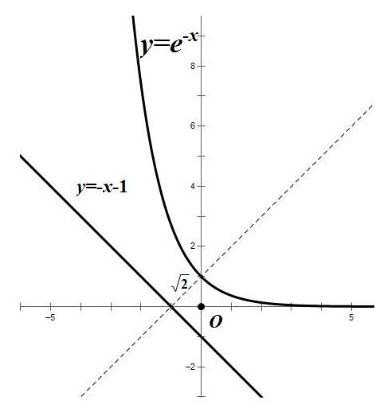
\includegraphics[max width=0.3\textwidth]{images/bo_d7fhnv491nqc73ercsbg_55_1049_300_385_409_0.jpg}
\end{center}
\hspace*{3em} 

\({f}^{\left( 2\right) }\left( x\right)  =  - a\sin \left( {x + t}\right)  - b\cos \left( {x + t}\right) ,\)

\({f}^{\left( 3\right) }\left( x\right)  =  - a\cos \left( {x + t}\right)  + b\sin \left( {x + t}\right) ,\)

\({f}^{\left( 4\right) }\left( x\right)  = a\sin \left( {x + t}\right)  + b\cos \left( {x + t}\right)  = f\left( x\right) ,\)

所以,对任意实数 \(a,b,t\) ,都有 \({f}^{\left( 4\right) }\left( x\right)  = f\left( x\right)\) .

(2)解: \(g\left( x\right)  = {e}^{mx} + n\cos x\) ，

\({g}^{\left( 1\right) }\left( x\right)  = m{e}^{mx} - n\sin x,{g}^{\left( 2\right) }\left( x\right)  = {m}^{2}{e}^{mx} - n\cos x,\)

由题意知, \({e}^{mx} + n\cos x = {m}^{2}{e}^{mx} - n\cos x\) 对任意实数 \(x\) 恒成立,

令 \(x = 0\) ,则 \(1 + n = {m}^{2} - n\) ,即 \({m}^{2} = 1 + {2n}\) ,

令 \(x = \frac{\pi }{2}\) ,则 \({e}^{\frac{m\pi }{2}} = {m}^{2}{e}^{\frac{m\pi }{2}}\) ,则 \({m}^{2} = 1\) ,

所以 \(m = 1,n = 0\) 或 \(m =  - 1,n = 0\) .

若 \(m = 1,n = 0\) ,则 \(g\left( x\right)  = {e}^{x},{g}^{\left( 1\right) }\left( x\right)  = {\mathrm{e}}^{x} = g\left( x\right)\) ,最小导周期不是 2,矛盾;

若 \(m =  - 1,n = 0\) ,则 \(g\left( x\right)  = {e}^{-x},{g}^{\left( 1\right) }\left( x\right)  =  - {\mathrm{e}}^{-x},{g}^{\left( 2\right) }\left( x\right)  = {\mathrm{e}}^{-x} = g\left( x\right)\) ,最小导周期为 2, 符合要求,所以 \(g\left( x\right)  = {e}^{-x}\) .

\(M\left( {a,b}\right)  = \sqrt{{\left( a - b\right) }^{2} + {\left( a + 1 + g\left( b\right) \right) }^{2}} = \sqrt{{\left( a - b\right) }^{2} + {\left( -a - 1 - {e}^{-b}\right) }^{2}}\) 可视为点 \(P\left( {a, - a - 1}\right)\) 与点 \(Q\left( {b,{e}^{-b}}\right)\) 之间的距离,当实数 \(a,b\) 变化时,点 \(P\left( {a, - a - 1}\right)\) 在直线 \(y =  - x - 1\) 上运动, 点 \(Q\left( {b,{e}^{-b}}\right)\) 在曲线 \(y = {e}^{-x}\) 上运动,因此所求最小值可转化为曲线 \(y = {e}^{-x}\) 上的点到直线 \(y =  - x - 1\) 距离的最小值,而曲线 \(y = {e}^{-x}\) 在直线 \(y =  - x - 1\) 上方,平移直线 \(y =  - x - 1\) 使其与曲线 \(y = {e}^{-x}\) 相切,

则切点到直线 \(y =  - x - 1\) 的距离即为所求.

设切点 \(M\left( {{x}_{0},{e}^{-{x}_{0}}}\right) ,{y}^{\prime } =  - {e}^{-x}\) ,切线斜率 \(- {e}^{-{x}_{0}} =  - 1\) ,得 \({x}_{0} = 0\) ,切点为 \(\left( {0,1}\right)\) , 点 \(\left( {0,1}\right)\) 到直线 \(y =  - x - 1\) 距离 \(d = \frac{\left| 1 + 0 + 1\right| }{\sqrt{{1}^{2} + {1}^{2}}} = \sqrt{2}\) . 即 \(M\left( {a,b}\right)\) 的最小值为 \(\sqrt{2}\) .

(3)解: \({h}^{\left( 1\right) }\left( x\right)  =  - \omega \sin \left( {\omega x}\right)\) ， \({h}^{\left( 2\right) }\left( x\right)  =  - {\omega }^{2}\cos \left( {\omega x}\right)\) ，

记 \(\varphi \left( x\right)  = {h}^{\left( 2\right) }\left( x\right)  - x\) ,即 \(\varphi \left( x\right)  =  - {\omega }^{2}\cos {\omega x} - x\) .

由 \(\varphi \left( x\right)  = {h}^{\left( 2\right) }\left( x\right)  - x \leq  0\) 在 \(\left( {0, + \infty }\right)\) 上恒成立及存在 \({x}_{0} > 0\) 使 \(\varphi \left( {x}_{0}\right)  = {h}^{\left( 2\right) }\left( {x}_{0}\right)  - {x}_{0} = 0\) ,可知 \(x = {x}_{0}\) 是函数 \(y = \varphi \left( x\right)\) 的极大值点,于是 \({\varphi }^{\prime }\left( {x}_{0}\right)  = {\omega }^{3}\sin \omega {x}_{0} - 1 = 0\) ,

则 \(\sin \omega {x}_{0} = \frac{1}{{\omega }^{3}}\)  \circled{1} ,

又 \(\varphi \left( {x}_{0}\right)  =  - {\omega }^{2}\cos \omega {x}_{0} - {x}_{0} = 0\) ,则 \(\cos \omega {x}_{0} = \frac{-{x}_{0}}{{\omega }^{2}}\)  \circled{2} ,

\({\mathbb{O}}^{2} + {@}^{2}\) ,得 \(\frac{1}{{\omega }^{6}} + \frac{{x}_{0}{}^{2}}{{\omega }^{4}} = 1\) ,则 \({x}_{0} = \frac{\sqrt{{\omega }^{6} - 1}}{\omega }\) .

又因为 \(\sin \omega {x}_{0} = \frac{1}{{\omega }^{3}} > 0,\cos \omega {x}_{0} = \frac{-{x}_{0}}{{\omega }^{2}} < 0\) ,

所以 \({2k\pi } + \frac{\pi }{2} < \omega {x}_{0} < {2k\pi } + \pi \left( {k \in  \mathbf{Z}}\right)\) ,由 \(\omega {x}_{0} > 0\) 得 \(k \geq  0\) ,

又因为 \(\frac{\pi }{2\omega } < {x}_{0} - \frac{2k\pi }{\omega } < \frac{\pi }{\omega }\left( {k \in  \mathbf{Z}}\right)\) ,

所以

\(\varphi \left( {{x}_{0} - \frac{2k\pi }{\omega }}\right)  =  - {\omega }^{2}\cos \left\lbrack  {\omega \left( {{x}_{0} - \frac{2k\pi }{\omega }}\right) }\right\rbrack   - \left( {{x}_{0} - \frac{2k\pi }{\omega }}\right)  =  - {\omega }^{2}\cos \omega {x}_{0} - {x}_{0} + \frac{2k\pi }{\omega } = \frac{2k\pi }{\omega } \leq  0,\)

有 \(k \leq  0\) ,于是 \(k = 0\) ,

所以 \(\frac{\pi }{2\omega } < {x}_{0} < \frac{\pi }{\omega }\) .

23.(2025 高三二模青浦 21)函数的导函数有很多有趣的性质，例如:函数 \(y = c\) (实数 \(c\) 为常数) 的导函数为 \(y = 0\) ; 反之,若函数 \(y = \phi \left( x\right)\) 的导函数为 \({\phi }^{\prime }\left( x\right)  = 0\) ,则 \(\phi \left( x\right)  = c\) (实数 \(c\) 为常数).

已知函数 \(y = f\left( x\right)\) 与 \(y = g\left( x\right)\) 定义域都是 \(\mathbf{R}\) ,导函数分别为 \(y = {f}^{\prime }\left( x\right)\) 和 \(y = {g}^{\prime }\left( x\right)\) .

若 \({f}^{\prime }\left( x\right)  = f\left( x\right)\) ,则称 \(y = f\left( x\right)\) 是 “自导函数”; 若 \({f}^{\prime }\left( x\right)  = g\left( x\right)\) 且 \({g}^{\prime }\left( x\right)  =  - f\left( x\right)\) ,则称 \(y = f\left( x\right)\) 与 \(y = g\left( x\right)\) 是 “共轭互导函数”.

(1)请判断函数 \(y = {\mathrm{e}}^{{ax} + b}\left( {a,b \in  \mathbf{R},a \neq  0}\right)\) 是否是“自导函数”，并说明理由；

( 2 )若函数 \(y = f\left( x\right)\) 是“自导函数”，且满足 \(f\left( 0\right)  = 1\) ，求证: \(f\left( x\right) f\left( {-x}\right)  = 1\) ；

(3)若函数 \(y = f\left( x\right)\) 与 \(y = g\left( x\right)\) 是 “共轭互导函数”，满足 \(f\left( 0\right)  = 0\) ， \(g\left( 0\right)  = 1\) ，求证: \({f}^{2}\left( x\right)  + {g}^{2}\left( x\right)  = 1\) . 进而证明 \(f\left( x\right)  = \sin x\) 且 \(g\left( x\right)  = \cos x\) .

【答案】(1) 当 \(a = 1\) 时, \(y = {\mathrm{e}}^{{ax} + b}\) 是 “自导函数”,当 \(a \neq  1\) 时, \(y = {\mathrm{e}}^{{ax} + b}\) 不是 “自导函数”;

(2)证明见解析:(3)证明见解析

【解析】(1) 对函数 \(y = {\mathrm{e}}^{{ax} + b}\) 求导,得 \({y}^{\prime } = a{\mathrm{e}}^{{ax} + b}\) .

当 \(a = 1\) 时， \(y = {\mathrm{e}}^{{ax} + b}\) 是 “自导函数”；

当 \(a \neq  1\) 时， \(y = {\mathrm{e}}^{{ax} + b}\) 不是 “自导函数”.

(2)因为函数 \(y = f\left( x\right)\) 是“自导函数”，

所以 \({f}^{\prime }\left( x\right)  = f\left( x\right)\) ,同时 \({f}^{\prime }\left( {-x}\right)  = f\left( {-x}\right)\) .

记 \(F\left( x\right)  = f\left( x\right) f\left( {-x}\right)\) ,求导,得

\({F}^{\prime }\left( x\right)  = {f}^{\prime }\left( x\right) f\left( {-x}\right)  + f\left( x\right) {\left( f\left( -x\right) \right) }^{\prime }\)

\(= {f}^{\prime }\left( x\right) f\left( {-x}\right)  - f\left( x\right) {f}^{\prime }\left( {-x}\right)\)

\(= f\left( x\right) f\left( {-x}\right)  - f\left( x\right) f\left( {-x}\right)  = 0,\)

即 \({F}^{\prime }\left( x\right)  = 0\) .

根据已知条件得 \(F\left( x\right)  = c\) (实数 \(c\) 为常数).

又 \(f\left( 0\right)  = 1\) ,所以 \(F\left( 0\right)  = f\left( 0\right) f\left( {-0}\right)  = 1\) ,

故 \(c = 1\) ,于是 \(f\left( x\right) f\left( {-x}\right)  = 1\) .

(3)易得 \({\left( {f}^{2}\left( x\right) \right) }^{\prime } = {\left( f\left( x\right) f\left( x\right) \right) }^{\prime } = {f}^{\prime }\left( x\right) f\left( x\right)  + f\left( x\right) {f}^{\prime }\left( x\right)  = {2f}\left( x\right) {f}^{\prime }\left( x\right)\) ，

设 \(G\left( x\right)  = {f}^{2}\left( x\right)  + {g}^{2}\left( x\right)\) ,

于是 \({G}^{\prime }\left( x\right)  = {2f}\left( x\right) {f}^{\prime }\left( x\right)  + {2g}\left( x\right) {g}^{\prime }\left( x\right)\) .

因为函数 \(y = f\left( x\right)\) 与 \(y = g\left( x\right)\) 是 “共轭互导函数”,

所以 \({f}^{\prime }\left( x\right)  = g\left( x\right)\) 且 \({g}^{\prime }\left( x\right)  =  - f\left( x\right)\) ,

于是 \({G}^{\prime }\left( x\right)  = {2f}\left( x\right) g\left( x\right)  - {2g}\left( x\right) f\left( x\right)  = 0\) ,

故 \(G\left( x\right)  = c\) (实数 \(c\) 为常数).

而 \(G\left( 0\right)  = {f}^{2}\left( 0\right)  + {g}^{2}\left( 0\right)  = 1\) ,

所以 \({f}^{2}\left( x\right)  + {g}^{2}\left( x\right)  = 1\) .

下面证明 \(f\left( x\right)  = \sin x\) 且 \(g\left( x\right)  = \cos x\) .

首先,容易验证 \(y = \sin x\) 和 \(y = \cos x\) 是一对满足条件的“共轭互导函数”.

接着证明满足条件的函数只有 \(y = \sin x\) 和 \(y = \cos x\) .

用反证法. 假设除了 \(y = \sin x\) 和 \(y = \cos x\) 外,还存在满足条件的一对 “共轭互导函数” \(y = {f}_{1}\left( x\right)\) 与 \(y = {g}_{1}\left( x\right)\) ,即

\({f}_{1}^{\prime }\left( x\right)  = {g}_{1}\left( x\right) ,\;{g}_{1}^{\prime }\left( x\right)  =  - {f}_{1}\left( x\right)\) ,同时满足 \({f}_{1}\left( 0\right)  = 0,{g}_{1}\left( 0\right)  = 1\) .

令 \(\mu \left( x\right)  = {f}_{1}\left( x\right) \sin x + {g}_{1}\left( x\right) \cos x\) ,则

\({\mu }^{\prime }\left( x\right)  = {f}_{1}^{\prime }\left( x\right) \sin x + {f}_{1}\left( x\right) \cos x + {g}_{1}^{\prime }\left( x\right) \cos x + {g}_{1}\left( x\right) \left( {-\sin x}\right)\)

\(= {g}_{1}\left( x\right) \sin x + {f}_{1}\left( x\right) \cos x - {f}_{1}\left( x\right) \cos x + {g}_{1}\left( x\right) \left( {-\sin x}\right)  = 0\) ,

于是 \(\mu \left( x\right)  = c\) (实数 \(c\) 为常数).

又 \(\mu \left( 0\right)  = 1\) ,

所以 \(\mu \left( x\right)  = 1\) .

故 \({f}_{1}\left( x\right) \sin x + {g}_{1}\left( x\right) \cos x = 1\) ,(1)

再令 \(\tau \left( x\right)  = {f}_{1}\left( x\right) \cos x - {g}_{1}\left( x\right) \sin x\) ,则

\({\tau }^{\prime }\left( x\right)  = {f}_{1}^{\prime }\left( x\right) \cos x + {f}_{1}\left( x\right) \left( {-\sin x}\right)  - {g}_{1}^{\prime }\left( x\right) \sin x - {g}_{1}\left( x\right) \cos x = 0,\)

于是 \(\tau \left( x\right)  = c\) (实数 \(c\) 为常数).

又 \(\tau \left( 0\right)  = 0\) ,

所以 \(\tau \left( x\right)  = 0\) ,

故 \({f}_{1}\left( x\right) \cos x - {g}_{1}\left( x\right) \sin x = 0\) (2)

由(1)(2)，得

\({f}_{1}\left( x\right)  = \sin x\) 与 \({g}_{1}\left( x\right)  = \cos x\) .

由此, 满足条件的“共轭互导函数”只有一对,

所以 \(f\left( x\right)  = \sin x\) 且 \(g\left( x\right)  = \cos x\) .

24.(2025 高三二模虹口 21)对于定义在 \(\mathbf{R}\) 上的函数 \(y = f\left( x\right)\) 和 \(y = g\left( x\right) ,a \in  \mathbf{R}\) ，设 \({M}_{a} = \left\{  {t \mid  t = f\left( x\right)  - g\left( a\right) ,x \geq  a}\right\}  .\)

(1)若 \(f\left( x\right)  = {2}^{x} - 1,g\left( x\right)  = \cos x\) ，求 \({M}_{0}\) ；

(2)若 \(f\left( x\right)  = {x}^{3} - 3{x}^{2},g\left( x\right)  =  - x,{M}_{a} \subseteq  \lbrack 0, + \infty )\) ，求实数 \(a\) 的取值范围；

(3)已知对任意 \(a \in  \mathbf{R}\) ，均有 \({M}_{a} = \lbrack 0, + \infty )\) ，记 \(h\left( x\right)  = g\left( x\right)  - a\) ，求证:“对任意 \(a \in  \mathbf{R}\) ，函数 \(y = h\left( x\right)\) 零点个数均有限”的充要条件是 “ \(y = f\left( x\right)\) 是严格增函数”.

【答案】( 1 ) \({M}_{0} = \lbrack  - 1, + \infty )\) ；( 2 ) \(a \geq  \frac{3 + \sqrt{5}}{2}\) ；( 3 )证明见解析

【解析】( 1 )记 \(F\left( x\right)  = f\left( x\right)  - g\left( 0\right)  = {2}^{x} - 1 - \cos 0 = {2}^{x} - 2\) ， .2 分函数 \(y = F\left( x\right) ,x \geq  0\) 上的值域为 \(\lbrack  - 1, + \infty )\) ,即 \({M}_{0} = \lbrack  - 1, + \infty )\) . .4 分

(2)设 \(G\left( x\right)  = f\left( x\right)  - g\left( a\right)  = {x}^{3} - 3{x}^{2} + a\) 在 \(x \in  \lbrack a, + \infty )\) 上的最小值 \({G}_{\min } \geq  0\) .

\({G}^{\prime }\left( x\right)  = 3{x}^{2} - {6x} = {3x}\left( {x - 2}\right) .\)

当 \(x \in  \left( {-\infty ,0}\right)\) 时, \({G}^{\prime }\left( x\right)  > 0,G\left( x\right)\) 严格增; 当 \(x \in  \left( {0,2}\right)\) 时, \({G}^{\prime }\left( x\right)  < 0,G\left( x\right)\) 严格减;

当 \(x \in  \left( {2, + \infty }\right)\) 时, \({G}^{\prime }\left( x\right)  > 0,G\left( x\right)\) 严格增. 当 \(x = 2\) 时 \(G\left( x\right)\) 取得极小值. .6 分

当 \(a \leq  2\) 时, \(\left\{  {\begin{array}{l} G\left( a\right)  \geq  0 \\  G\left( 2\right)  \geq  0 \end{array} \Rightarrow  \left\{  {\begin{array}{l} {a}^{3} - 3{a}^{2} + a \geq  0 \\   - 4 + a \geq  0 \end{array} \Rightarrow  \left\{  \begin{array}{l} a\left( {{a}^{2} - {3a} + 1}\right)  \geq  0, \\  a \geq  4, \end{array}\right. }\right. }\right.\) 舍去. .8 分

当 \(a > 2\) 时， \(G\left( a\right)  \geq  0 \Rightarrow  a\left( {{a}^{2} - {3a} + 1}\right)  \geq  0,a \geq  \frac{3 + \sqrt{5}}{2}\) . .10 分

综上， \(a \geq  \frac{3 + \sqrt{5}}{2}\) .

(3)(充分性)若 \(y = f\left( x\right)\) 是严格增函数，则 \(y = f\left( x\right)  - g\left( a\right) ,x \geq  a\) 的最小值为 \(f\left( a\right)  - g\left( a\right)\) ， 而 \({M}_{a} = \lbrack 0, + \infty )\) ,故对任意 \(a \in  \mathbf{R}\) ,都有 \(f\left( a\right)  = g\left( a\right)\) ,即 \(y = g\left( x\right)\) 与 \(y = f\left( x\right)\) 是相同函数. .12 分故 \(y = g\left( x\right)\) 是严格增函数,所以 \(y = h\left( x\right)\) 严格增函数,故对任意 \(a \in  \mathbf{R},h\left( x\right)  = g\left( x\right)  - a\) 的零点个数有限.

(必要性) 对任意 \(a \in  \mathbf{R}\) ,都有 \({M}_{a} = \lbrack 0, + \infty )\) ,故 \(y = f\left( x\right) ,x \geq  a\) 的值域为 \(\lbrack g\left( a\right) , + \infty )\) ,即 \(y = f\left( x\right)\) 在 \(x \in  \lbrack a, + \infty )\) 上的最小值为 \(g\left( a\right)\) .

先证 \(y = g\left( x\right)\) 是严格增函数.

对任意 \({a}_{1} < {a}_{2}\) ,函数 \(y = f\left( x\right) ,x \geq  {a}_{1}\) 和 \(y = f\left( x\right) ,x \geq  {a}_{2}\) 的最小值分别为 \(g\left( {a}_{1}\right)\) 和 \(g\left( {a}_{2}\right)\) ,则由最小值的定义, \(g\left( {a}_{1}\right)  \leq  g\left( {a}_{2}\right)\) ,故函数 \(y = g\left( x\right)\) 是增函数. .14 分假设存在 \({a}_{1} < {a}_{2}\) ,使得 \(g\left( {a}_{1}\right)  = g\left( {a}_{2}\right)\) ,则对任意 \(x \in  \left\lbrack  {{a}_{1},{a}_{2}}\right\rbrack\) ,均有 \(g\left( {a}_{1}\right)  \leq  g\left( x\right)  \leq  g\left( {a}_{2}\right)\) ,从而方程 \(g\left( x\right)  = g\left( {a}_{2}\right)\) 的解有无限多个,与条件“对任意 \(a \in  \mathbf{R}\) ,函数 \(y = h\left( x\right)\) 零点个数均有限”矛盾. 故假设不成立,从而 \(y = g\left( x\right)\) 是严格增函数. .16 分再证对任意 \(a \in  \mathbf{R}\) ,函数 \(y = f\left( x\right) ,x \geq  a\) 的最小值为 \(f\left( a\right)\) .

假设存在 \({x}_{0} > a\) 使得 \(f\left( {x}_{0}\right)  = g\left( a\right)\) ,取 \(c \in  \left( {a,{x}_{0}}\right)\) ,则 \(y = f\left( x\right) ,x \geq  c\) 的最小值为 \(g\left( c\right)\) . 由 \(y = g\left( x\right)\) 严格增,知 \(g\left( c\right)  > g\left( a\right)\) . 而 \({x}_{0} \in  \lbrack c, + \infty )\) ,故 \(f\left( {x}_{0}\right)  \geq  g\left( c\right)  > g\left( a\right)\) ,矛盾. 所以假设不成立,对任意 \(a \in  \mathbf{R}\) ,函数 \(y = f\left( x\right) ,x \geq  a\) 的最小值为 \(f\left( a\right)\) .

而对任意 \(a \in  \mathbf{R},y = f\left( x\right) ,x \geq  a\) 的值域为 \(\lbrack g\left( a\right) , + \infty )\) ,故 \(f\left( a\right)  = g\left( a\right)\) . 于是 \(y = g\left( x\right)\) 与 \(y = f\left( x\right)\) 是相同函数,所以 \(y = f\left( x\right)\) 是严格增函数. .18 分

25.(2025 高三二模黄浦 21)设 \(D\) 是 \(\mathbf{R}\) 的一个非空子集，函数 \(y = f\left( x\right)\) 的定义域为 \(D\) ，若 \(y = f\left( x\right)\) 在 \(D\) 上不是单调函数,且存在常数 \(b\) ,使得 \(f\left( x\right)  \geq  b\) 对任意的 \(x \in  D\) 成立,则称函数 \(y = f\left( x\right)\) 具有性质 \(H\) ,称 \(b\) 为该函数的一个下界.

(1)设 \(f\left( x\right)  = x + \frac{1}{x},D = \left( {-\infty ,0}\right)\) ，判断函数 \(y = f\left( x\right)\) ， \(x \in  D\) 是否具有性质 \(H\) ；

(2)设 \(m\) 为常数， \(f\left( x\right)  = \frac{1}{3}{x}^{3} - x + 1,D = \left( {m,2}\right)\) ，当且仅当 \(m\) 满足什么条件时，函数 \(y = f\left( x\right) ,x \in  D\) 具有性质 \(H\) ,且 \(b = \frac{1}{3}\) 是该函数的一个下界;

(3)设 \(0 < a \leq  1,f\left( x\right)  = \ln \left( {x + 1}\right)  + {ax}\left( {x - 2}\right) ,D = \left( {0,1}\right)\) ,若函数 \(y = f\left( x\right) ,x \in  D\) 具有性质 \(H\) ,求 \(a\) 的取值范围: 当 \(a\) 在上述范围内变化时,若 \(b\) 总是该函数的下界,求 \(b\) 的取值范围.

【答案】(1) 不具有; (2) \(m \in  \lbrack  - 2,1);\left( 3\right) \frac{1}{2} < a \leq  1,b \leq  \ln \frac{2 + \sqrt{2}}{2} - \sqrt{2} + \frac{1}{2}\) .

【解析】(1) 函数 \(f\left( x\right)  = x + \frac{1}{x},x \in  \left( {-\infty ,0}\right)\) ,求导得 \({f}^{\prime }\left( x\right)  = 1 - \frac{1}{{x}^{2}} = \frac{{x}^{2} - 1}{{x}^{2}}\) ,

当 \(x \in  \left( {-\infty , - 1}\right)\) 时, \({f}^{\prime }\left( x\right)  > 0\) ; 当 \(x \in  \left( {-1,0}\right)\) 时, \({f}^{\prime }\left( x\right)  < 0\) ,

函数 \(f\left( x\right)\) 在 \(\left( {-\infty , - 1}\right)\) 上单调递增, \(\left( {-1,0}\right)\) 上单调递减,

于是函数 \(y = f\left( x\right)\) 在 \(\left( {-\infty ,0}\right)\) 上不是单调函数, \(\forall x \in  \left( {-\infty ,0}\right) ,f\left( x\right)  \leq  f\left( {-1}\right)  =  - 2\) ,

函数 \(f\left( x\right)\) 在 \(\left( {-\infty ,0}\right)\) 上的值域为 \(( - \infty , - 2\rbrack\) ,

不存在常数 \(b\) ,使得 \(f\left( x\right)  \geq  b\) 对任意的 \(x \in  \left( {-\infty ,0}\right)\) 成立,

所以函数 \(y = f\left( x\right) ,x \in  D\) 不具有性质 \(H\) .

(2)函数 \(f\left( x\right)  = \frac{1}{3}{x}^{3} - x + 1\) ，求导得 \({f}^{\prime }\left( x\right)  = {x}^{2} - 1 = \left( {x + 1}\right) \left( {x - 1}\right)\) ，

当 \(x <  - 1\) 或 \(x > 1\) 时， \({f}^{\prime }\left( x\right)  > 0\) ；当 \(- 1 < x < 1\) 时， \({f}^{\prime }\left( x\right)  < 0\) ，

函数 \(f\left( x\right)\) 在 \(\left( {-\infty , - 1}\right) ,\left( {1, + \infty }\right)\) 上单调递增,在 \(\left( {-1,1}\right)\) 上单调递减,

由函数 \(y = f\left( x\right) ,x \in  \left( {m,2}\right)\) 具有性质 \(H\) ,且 \(b = \frac{1}{3}\) 是该函数的一个下界,得 \(f{\left( x\right) }_{\min } \geq  \frac{1}{3}\) ,

当 \(m < 1\) 时,函数 \(y = f\left( x\right)\) 在 \(\left( {m,2}\right)\) 上不单调, \(f\left( {-1}\right)  = \frac{5}{3},f\left( 1\right)  = \frac{1}{3}\) ,

由 \(f\left( x\right)  = \frac{1}{3}\) ,即 \({x}^{3} - {3x} + 2 = 0\) ,整理得 \(\left( {x + 2}\right) {\left( x - 1\right) }^{2} = 0\) ,解得 \(x =  - 2\) 或 \(x = 1\) ,

当 \(x <  - 2\) 时, \(f\left( x\right)  < f\left( {-2}\right)  = \frac{1}{3}\) ,当 \(- 2 \leq  x < 1\) 时, \(f\left( x\right)  \geq  f\left( {-2}\right)  = \frac{1}{3}\) ,

因此 \(\forall x \in  \lbrack  - 2,1),f\left( x\right)  \geq  \frac{1}{3}\) ,则 \(- 2 \leq  m < 1\) ,

所以当且仅当 \(m \in  \lbrack  - 2,1)\) 时,函数 \(y = f\left( x\right) ,x \in  D\) 具有性质 \(H\) ,且 \(b = \frac{1}{3}\) 是该函数的一个下界.

(3)当 \(a \in  (0,1\rbrack ,x \in  \left( {0,1}\right)\) 时，函数 \(f\left( x\right)  = \ln \left( {x + 1}\right)  + a{x}^{2} - {2ax}\) ， 求导得 \({f}^{\prime }\left( x\right)  = \frac{1}{x + 1} + {2ax} - {2a} = \frac{{2a}{x}^{2} - \left( {{2a} - 1}\right) }{x + 1}\) ,

当 \(0 < a \leq  \frac{1}{2}\) 时, \({2a} - 1 \leq  0,{f}^{\prime }\left( x\right)  > 0\) ,函数 \(f\left( x\right)\) 在 \(\left( {0,1}\right)\) 上单调递增,不符合题意; 当 \(\frac{1}{2} < a \leq  1\) 时, \(0 < {2a} - 1 \leq  1\) ,由 \({f}^{\prime }\left( x\right)  < 0\) ,得 \(0 < x < \sqrt{1 - \frac{1}{2a}}\) ; 由 \({f}^{\prime }\left( x\right)  > 0\) ,得 \(\sqrt{1 - \frac{1}{2a}} < x < 1\)

函数 \(f\left( x\right)\) 在 \(\left( {0,\sqrt{1 - \frac{1}{2a}}}\right)\) 上单调递减,在 \(\left( {\sqrt{1 - \frac{1}{2a}},1}\right)\) 上单调递增, \(f\left( x\right)\) 在 \(\left( {0,1}\right)\) 上不是单调函数,

\(f{\left( x\right) }_{\min } = f\left( \sqrt{1 - \frac{1}{2a}}\right)  = \ln \left( {\sqrt{1 - \frac{1}{2a}} + 1}\right)  + a - \frac{1}{2} - {2a}\sqrt{1 - \frac{1}{2a}},b \leq  f{\left( x\right) }_{\min }\) ,因此 \(\frac{1}{2} < a \leq  1\)

令 \(\sqrt{1 - \frac{1}{2a}} = t \in  \left( {0,\frac{\sqrt{2}}{2}}\right\rbrack\) ,则 \({2a} = \frac{1}{1 - {t}^{2}}\) ,令 \(g\left( t\right)  = f\left( \sqrt{1 - \frac{1}{2a}}\right)  = \ln \left( {t + 1}\right)  + \frac{1 - {2t}}{2\left( {1 - {t}^{2}}\right) } - \frac{1}{2}\) , 求导得 \({g}^{\prime }\left( t\right)  = \frac{1}{1 + t} + \frac{-2\left( {1 - {t}^{2}}\right)  - \left( {1 - {2t}}\right) \left( {-{2t}}\right) }{2{\left( 1 - {t}^{2}\right) }^{2}} = \frac{{t}^{3} - 2{t}^{2}}{{\left( 1 - {t}^{2}\right) }^{2}} < 0\) , 函数 \(g\left( t\right)\) 在 \(\left( {0,\frac{\sqrt{2}}{2}}\right\rbrack\) 上单调递减， \(g{\left( t\right) }_{\min } = g\left( \frac{\sqrt{2}}{2}\right)  = \ln \frac{2 + \sqrt{2}}{2} - \sqrt{2} + \frac{1}{2}\) ， 由当 \(a\) 变化时, \(b\) 总是该函数的下界,得 \(b \leq  g{\left( t\right) }_{\min } = \ln \frac{2 + \sqrt{2}}{2} - \sqrt{2} + \frac{1}{2}\) , 所以 \(a\) 的取值范围是 \(\frac{1}{2} < a \leq  1,b\) 的取值范围是 \(b \leq  \ln \frac{2 + \sqrt{2}}{2} - \sqrt{2} + \frac{1}{2}\) .

\section*{八、函数实际应用问题与数学建模}

1.(2025 高三二模宝山 11)某分公司经销一产品，每件产品的成本为 5 元，且每件产品需向总公司交 2 元的管理费,预计每件产品的售价为 \(x\) 元 \(\left( {8 \leq  x \leq  {11}}\right)\) 时,一年的销售量为 \({\left( {12} - x\right) }^{2}\) 万件，则每件产品售价为\_\_\_\_\_元时，该分公司一年的利润达到最大值.(结果精确到 1 元)

【答案】 9

【解析】设利润为 \(W = \left( {x - 7}\right) {\left( {12} - x\right) }^{2}\) ,化简可得 \(W = {x}^{3} - {31}{x}^{2} + {312x} - {1008}\) , \({W}^{\prime } = 3{x}^{2} - {62x} + {312}\) ,令 \({W}^{\prime } = 0\) ,解得 \(x = \frac{26}{3}\) 或 \(x = {12}\) , 因为 \(8 \leq  x \leq  {11}\) ,当 \(8 \leq  x < \frac{26}{3}\) 时, \({W}^{\prime } > 0\) ,函数严格递增,当 \(\frac{26}{3} < x \leq  {11}\) 时, \({W}^{\prime } < 0\) , 函数严格递减,所以利润在 \(x = \frac{26}{3} \approx  9\) 时,取得最大值.

2.(2025 高三二模虹口 11)1798 年，人口学家马尔萨斯假设:单位时间内的人口增长量 \({x}^{\prime }\left( t\right)\) 与人口数 \(x\left( t\right)\) 成正比,进而建立马尔萨斯人口增长模型.19 世纪中叶的生物学家们发现由于人类生存条件的限制，存在人口最大瞬时增长率 \({r}_{0}\) ，当达到 \({r}_{0}\) 时，人口增长率 \(r\) 会随着 \(x\left( t\right)\) 的增长而下降，因此需要改进马尔萨斯的假设. 他们假设: \circled{1}  \(x\left( t\right)\) 是随着时间 \(t\) 连续变化的函数;  \circled{2} 存在最大人口数 \(N\) ，人口数达到 \(N\) 时， \(r = 0\) ； \circled{3}  \({x}^{\prime }\left( t\right)\) 仅与 \(r\) 和 \(x\left( t\right)\) 有关； \circled{4}  \(r = {r}_{0} - k \cdot  x\left( t\right) \left( {k > 0}\right)\) ,那么在这些条件下建立的人口增长模型 \({x}^{\prime }\left( t\right)  =\) \_\_\_\_\_. (用含有 \(x\left( t\right) \text{ 、 }{r}_{0}\text{ 、 }N\) 的式子表示)

【答案】 \({r}_{0}x\left( t\right) \left( {1 - \frac{x\left( t\right) }{N}}\right)\)

【解析】人口数为 \(x\left( t\right)\) ,人口增长率为: \(r = {r}_{0} - k \cdot  x\left( t\right) \left( *\right)\) ,

由题意知单位时间人口增长量为 \({x}^{\prime }\left( t\right)\) ,

当 \(x\left( t\right)  = N\) 时, \(r = 0\) ,代入 (*) 式得 \(k = \frac{{r}_{0}}{N}\) ,

\(\therefore {x}^{\prime }\left( t\right)  = r \cdot  x\left( t\right)  = \left\lbrack  {{r}_{0} - k \cdot  x\left( t\right) }\right\rbrack   \cdot  x\left( t\right)  = \left\lbrack  {{r}_{0} - \frac{{r}_{0}}{N} \cdot  x\left( t\right) }\right\rbrack   \cdot  x\left( t\right)\)

\(= {r}_{0}x\left( t\right) \left( {1 - \frac{x\left( t\right) }{N}}\right) .\)

3. (2025 高三二模青浦 11) 道路通行能力指单位时间 (1 小时) 内通过道路上指定断面的最大车辆数, 是度量道路疏导交通能力的指标. 同时为了行驶安全, 车辆之间必须保持一定的安全距离. 为了研究某城市道路通行能力, 现给出如下假设:

假设 1: 车身长度均为 4.8 米;

假设 2: 所有车辆以相同的速度 \(v\) (单位: 千米/小时)匀速行驶;

假设 3: 安全距离 \(d\) (单位: 米)与车辆速度 \(v\) 近似满足 \(d = {3.2} + {0.6522v} + {0.01}{v}^{2}\) . 该城市道路通行能力的最大值为\_\_\_\_\_.(结果保留整数)

【答案】821

【解析】每辆车占的长度为 \({4.8} + {3.2} + {0.6522v} + {0.01}{v}^{2} = {0.01}{v}^{2} + {0.6522v} + 8\) 通行能力为

\[
N = \frac{1000v}{{0.01}{v}^{2} + {0.6522v} + 8} = \frac{1000}{{0.01v} + \frac{8}{v} + {0.6522}} \leq  \frac{1000}{2\sqrt{{0.01v} \cdot  \frac{8}{v}} + {0.6522}} \approx  {821.1},
\]

当且仅当 \({0.01v} = \frac{8}{v}\) 时取等号.

\section*{第三部分 三角与三角函数}

\section*{一、三角定义、常用三角公式}

1. (2025 高三二模虹口 3)若 \(\sin \alpha  = \frac{2}{3}\) ，则 \(\cos {2\alpha } =\) \_\_\_\_\_.

【答案】 \(\frac{1}{9}\)

【解析】 \(\cos {2\alpha } = 1 - 2{\sin }^{2}\alpha  = 1 - 2 \times  {\left( \frac{2}{3}\right) }^{2} = \frac{1}{9}\) .

2.(2025 高三二模杨浦 4)已知 \(\sin \alpha  = \frac{3}{5}\) ，则 \(\cos {2\alpha } =\) \_\_\_\_\_.

【答案】 \(\frac{7}{25}\)

【解析】 \(\cos {2\alpha } = 1 - 2{\sin }^{2}\alpha  = \frac{7}{25}\) .

3. (2025 高三二模金山 4)已知角 \(x\) 在第二象限，且 \(\sin x = \frac{4}{5}\) ，则 \(\tan x =\) \_\_\_\_\_.

【答案】 \(- \frac{4}{3}\)

【解析】由题意知 \(\cos x =  - \frac{3}{5},\therefore \tan x =  - \frac{4}{3}\) .

4.(2025 高三二模徐汇 6)已知 \(\cos \theta  =  - \frac{3}{5},\theta  \in  \left( {0,\pi }\right)\) ，则 \(\tan \left( {\theta  - \frac{\pi }{4}}\right)\) 的值为\_\_\_\_\_.

【答案】 7

【解析】由题意知 \(\sin \theta  = \frac{4}{5},\tan \theta  =  - \frac{4}{3},\tan \left( {\theta  - \frac{\pi }{4}}\right)  = \frac{\tan \theta  - 1}{1 + \tan \theta } = \frac{-\frac{4}{3} - 1}{1 + \left( {-\frac{4}{3}}\right) } = 7\) .

5.(2025 高三二模闵行 6)已知 \(\overrightarrow{a} = \left( {3,4}\right)\) ， \(\overrightarrow{b} = \left( {\cos \alpha ,\sin \alpha }\right)\) ，且 \(\overrightarrow{a}\) 与 \(\overrightarrow{b}\) 平行，则 \(\tan \alpha  =\) \_\_\_\_\_.

【答案】 \(\frac{4}{3}\)

【解析】由题意知 \(4\cos \alpha  = 3\sin \alpha  \Rightarrow  \tan \alpha  = \frac{4}{3}\) .

6.(2025 高三二模静安 6)已知 \(\sin \left( {\frac{\pi }{4} - x}\right)  = \frac{3}{5}\) ，则 \(\sin {2x}\) 的值为\_\_\_\_\_.

【答案】 \(\frac{7}{25}\)

【解析】 \(\sin {2x} = \cos \left( {\frac{\pi }{2} - {2x}}\right)  = 1 - 2{\sin }^{2}\left( {\frac{\pi }{4} - x}\right)  = 1 - 2 \times  {\left( \frac{3}{5}\right) }^{2} = \frac{7}{25}\) .

7.(2025 高三二模嘉定 6)已知 \(\theta  \in  \mathbf{R}\) ，若 \(\tan \theta  + \cot \theta  = 5\) ，则 \(\sin {2\theta } =\) \_\_\_\_\_.

【答案】 \(\frac{2}{5}\)

【解析】 \(\tan \theta  + \cot \theta  = \frac{\sin \theta }{\cos \theta } + \frac{\cos \theta }{\sin \theta } = \frac{{\sin }^{2}\theta  + {\cos }^{2}\theta }{\sin \theta \cos \theta } = \frac{1}{\sin \theta \cos \theta } = 5\) , 所以 \(\sin \theta \cos \theta  = \frac{1}{5}\) ,则 \(\sin {2\theta } = 2\sin \theta \cos \theta  = \frac{2}{5}\) .

8.(2025 高三二模普陀 14)设 \(m \in  \mathbf{R}\) ，在平面直角坐标系 \({xOy}\) 中，角 \(\alpha\) 的顶点在坐标原点,始边与 \(x\) 轴的正半轴重合,若角 \(\alpha\) 的终边经过点 \(P\left( {-3,m}\right)\) ,且 \(\sin \left( {\pi  + {2\alpha }}\right)  > 0\) ,则角 \(\alpha\) 属于( )

A. 第一象限 B.第二象限 C.第三象限 D. 第四象限

【答案】B

【解析】由题意 \(\sin \alpha  = \frac{m}{r},\cos \alpha  = \frac{-3}{r}\) ,其中 \(r = \sqrt{{\left( -3\right) }^{2} + {m}^{2}}\) , \(\sin \left( {\pi  + {2\alpha }}\right)  =  - \sin {2\alpha } =  - 2\sin \alpha \cos \alpha  = \frac{6m}{{r}^{2}} > 0\) ,则 \(m > 0\) ,则点 \(P\) 在第二象限,所以角 \(\alpha\) 为第二象限角,故选 B.

\section*{二、三角方程}

1. (2025 高三二模虹口 18)已知函数 \(y = f\left( x\right)\) 的表达式为 \(f\left( x\right)  = {2}^{x},x \in  \mathbf{R}\) .

(1)解不等式: \({\log }_{2}\left\lbrack  {f\left( x\right)  - 1}\right\rbrack   + {\log }_{2}\left\lbrack  {f\left( x\right) }\right\rbrack   \leq  1\) ；

( 2 )若存在 \({x}_{0} \in  \left\lbrack  {0,\frac{\pi }{2}}\right\rbrack\) ，使得 \(f\left( {m\sin {x}_{0}}\right)\) ， \(f\left( {2 + \sin {2{x}_{0}}}\right)\) ， \(f\left( {m\cos {x}_{0}}\right)\) 成等比数列， 求实数 \(m\) 的最小值.

【答案】(1) \(x \in  (0,1\rbrack\) ; (2) 4

【解析】(1) \({\log }_{2}\left( {{2}^{x} - 1}\right)  + {\log }_{2}{2}^{x} \leq  1\) ,即 \({\log }_{2}\left\lbrack  {\left( {{2}^{x} - 1}\right)  \cdot  {2}^{x}}\right\rbrack   \leq  {\log }_{2}2\) . .2 分故 \(\left\{  \begin{array}{l} \left( {{2}^{x} - 1}\right)  \cdot  {2}^{x} \leq  2, \\  {2}^{x} - 1 > 0. \end{array}\right.\) .4 分

解得 \(x \in  (0,1\rbrack\) . .6 分

(2)由于 \(f\left( {m\sin {x}_{0}}\right) ,f\left( {2 + \sin 2{x}_{0}}\right) ,f\left( {m\cos {x}_{0}}\right)\) 成等比数列,故 \({\left( {2}^{2 + \sin 2{x}_{0}}\right) }^{2} = {2}^{m\sin {x}_{0}} \cdot  {2}^{m\cos {x}_{0}},\)

即 \(4 + 2\sin 2{x}_{0} = m\left( {\sin {x}_{0} + \cos {x}_{0}}\right)\) 对 \({x}_{0} \in  \left\lbrack  {0,\frac{\pi }{2}}\right\rbrack\) 有解. .8 分

令 \(t = \sin {x}_{0} + \cos {x}_{0} = \sqrt{2}\sin \left( {{x}_{0} + \frac{\pi }{4}}\right)  \in  \left\lbrack  {1,\sqrt{2}}\right\rbrack\) ,

所以 \(\sin 2{x}_{0} = 2\sin {x}_{0}\cos {x}_{0} = {t}^{2} - 1\) . .10 分

所以 \(m = \frac{4 + 2\sin 2{x}_{0}}{\sin {x}_{0} + \cos {x}_{0}} = \frac{2{t}^{2} + 2}{t} = {2t} + \frac{2}{t}\) 对 \(t \in  \left\lbrack  {1,\sqrt{2}}\right\rbrack\) 有解. .12 分

由于 \({2t} + \frac{2}{t} \geq  2\sqrt{{2t} \cdot  \frac{2}{t}} = 4\) ,等号当且仅当 \({2t} = \frac{2}{t}\) ,即 \(t = 1\) 时成立.

所以 \(m \in  \left\lbrack  {4,3\sqrt{2}}\right\rbrack\) ,故 \(m\) 的最小值为 4 . .14 分

\section*{三、解三角形}

1. (2025 高三二模黄浦 4)在 \(\bigtriangleup {ABC}\) 中，若 \(A = {45}^{ \circ  },B = {30}^{ \circ  },{BC} = 2\sqrt{6}\) ，则 \({AC} =\) \_\_\_\_\_.

【答案】 \(2\sqrt{3}\)

【解析】由正弦定理可得 \(\frac{BC}{\sin A} = \frac{AC}{\sin B} \Rightarrow  {AC} = 2\sqrt{3}\) .

2.(2025 高三二模青浦 6)已知 \(\bigtriangleup  {ABC}\) 的角 \(A\) 、 \(B\) 、 \(C\) 对应边长分别为 \(a = 4\) ， \(b = 5\) ， \(c = 6\) ，则 \(A =\) \_\_\_\_\_.

【答案】 \(\arccos \frac{3}{4}\)

【解析】 \(\cos A = \frac{{5}^{2} + {6}^{2} - {4}^{2}}{2 \times  5 \times  6} = \frac{3}{4},\therefore A = \arccos \frac{3}{4}\) .

3.(2025 高三二模奉贤 7)已知 \(\bigtriangleup  {ABC}\) ，“ \(A\) 、 \(B\) 、 \(C\) 成等差数列且 \(\sin A\) 、 \(\sin B\) 、 \(\sin C\) 成等比数列”是“ \(\bigtriangleup  {ABC}\) 是正三角形”的\_\_\_\_\_条件.

【答案】充要条件

【解析】必要性显然,充分性: \(\left\{  {\begin{array}{l} {2B} = A + C \\  A + B + C = \pi  \end{array} \Rightarrow  B = \frac{\pi }{3}}\right.\) ,又 \({\sin }^{2}B = \frac{3}{4} = \sin A\sin C =  - \frac{1}{2}\left\lbrack  {\cos \left( {A + C}\right)  - \cos \left( {A - C}\right) }\right\rbrack   =  - \frac{1}{2}\left\lbrack  {-\cos B - \cos \left( {A - C}\right) }\right\rbrack \; \therefore \cos \left( {A - C}\right)  = 1 \Rightarrow  A - C = 0 \Rightarrow  A = C = \frac{\pi }{3}\) , 故应该是充要条件.

4.(2025 高三二模虹口 7)若 \(\bigtriangleup  {ABC}\) 的三条边的长分别为4、5、6，则 \(\bigtriangleup  {ABC}\) 的外接圆面积为\_\_\_\_\_. (结果保留 \(\pi\) )

【答案】 \(\frac{64}{7}\pi\)

【解析】设角 \(A,B,C\) 对应的边是 \(4,5,6,\therefore \cos A = \frac{{5}^{2} + {6}^{2} - {4}^{2}}{2 \times  5 \times  6} = \frac{3}{4},\therefore \sin A = \frac{\sqrt{7}}{4}\) , \(\therefore {2R} = \frac{4}{\frac{\sqrt{7}}{4}} = \frac{16}{\sqrt{7}} \Rightarrow  R = \frac{8\sqrt{7}}{7} \Rightarrow  \pi {R}^{2} = \frac{64}{7}\pi\) .

5.(2025 高三二模长宁 8)顶角为 \({36}^{ \circ  }\) 的等腰三角形被称为黄金三角形，其底边和腰之比正好为黄金比 \(\varphi\) ,用黄金比 \(\varphi\) 表示 \(\cos {36}^{ \circ  } =\) \_\_\_\_\_.

【答案】 \(1 - \frac{1}{2}{\varphi }^{2}\) (或 \(\frac{1 + \varphi }{2}\) 或 \(\frac{\sqrt{\varphi  + 2}}{2}\) 或 \(\frac{1}{2\varphi }\) )

【解析】设等腰三角形的腰长为 \(a\) ,底边长为 \(b\) ,则 \(\frac{b}{a} = \varphi\) ,由余弦定理可得 \(\cos {36}^{ \circ  } = \frac{{a}^{2} + {a}^{2} - {b}^{2}}{2 \cdot  a \cdot  a} = 1 - \frac{1}{2}{\varphi }^{2}.\)

6.(2025 高三二模崇明 8)在 \(\bigtriangleup  {ABC}\) 中，若 \(c = 3\) ， \(C = \frac{\pi }{3}\) ，其面积为 \(\sqrt{3}\) ，则 \(a + b =\) \_\_\_\_\_.

【答案】 \(\sqrt{21}\)

【解析】由题意知 \({S}_{\bigtriangleup {ABC}} = \frac{1}{2}{ab}\sin \frac{\pi }{3} = \sqrt{3} \Rightarrow  {ab} = 4\) ，

又 \(\cos \frac{\pi }{3} = \frac{1}{2} = \frac{{a}^{2} + {b}^{2} - {c}^{2}}{2ab} \Rightarrow  {a}^{2} + {b}^{2} - {3}^{2} = {ab} \Rightarrow  {a}^{2} + {b}^{2} = {13}\) ,

\(\therefore {\left( a + b\right) }^{2} - {2ab} = {13} \Rightarrow  {\left( a + b\right) }^{2} = {21} \Rightarrow  a + b = \sqrt{21}\) .

7.(2025 高三二模长宁 10)已知点 \(D\) 、 \(E\) 分别是三角形 \({ABC}\) 的边 \({AC}\) 、 \({BC}\) 的中点，且 \({AE} = 2,{BD} = 3\) ，则三角形 \({ABC}\) 的面积的取值范围是\_\_\_\_\_.

【答案】 \((0,4\rbrack\)

【解析】如图,过 \(A\) 作 \({AF}//{BC},{AF} = {BC}\) ,过 \(F\) 作 \({FG}//{AE}\) 交 \({BC}\) 的延长线于 \(G\) ,

则四边形 \({AFGE}\) 、四边形 \({ABCF}\) 为平行四边形,连接 \({BF}\) , 则 \({AC},{BF}\) 互相平分,故 \(B,D,F\) 共线且 \(D\) 为 \({BF}\) 的中点, 而 \({AF} = {BC} = {EG}\) ，故 \({BG} = \frac{3}{2}{BC}\) ，故 \({S}_{\bigtriangleup {BFG}} = \frac{3}{2}{S}_{\bigtriangleup {ABC}}\) ，

\begin{center}
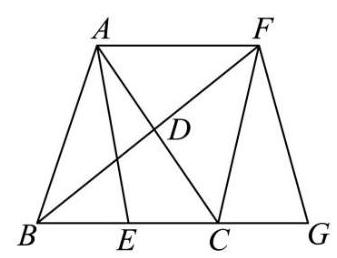
\includegraphics[max width=0.2\textwidth]{images/bo_d7fhnv491nqc73ercsbg_68_1068_1906_337_258_0.jpg}
\end{center}
\hspace*{3em} 

\(\bigtriangleup {BFG}\) 中, \({BF} = {2BD} = 6,{GF} = {AE} = 2,\angle {BFG} \in  \left( {0,\pi }\right)\) ,

故 \({S}_{\bigtriangleup {BFG}} = \frac{1}{2}{BF} \times  {FG}\sin \angle {BFG} = 6\sin \angle {BFG} \in  (0,6\rbrack\) ,

故 \({S}_{\bigtriangleup {ABC}} \in  (0,4\rbrack\) .

8. (2025 高三二模静安 12)在边长为 1 的正三角形 \({ABC}\) 的边 \({AB}\) 、 \({AC}\) 上分别取 \(D\) 、 \(E\) 两点,若沿线段 \({DE}\) 折叠该三角形时,顶点 \(A\) 恰好落在边 \({BC}\) 上. 则线段 \({AD}\) 的长度的最小值为\_\_\_\_\_.

【答案】 \(2\sqrt{3} - 3\)

【解析】设 \(A\) 落在 \({A}^{\prime },{AD} = x,\angle {ADE} = \theta\) ,则 \({BD} = 1 - x,D{A}^{\prime } = x,\angle {BD}{A}^{\prime } = \pi  - {2\theta }\) , 在 \(\bigtriangleup {A}^{\prime }{BD}\) 中,由正弦定理得 \(\frac{{A}^{\prime }D}{\sin B} = \frac{BD}{\sin \angle B{A}^{\prime }D}\) ,即 \(\frac{x}{\sin \frac{\pi }{3}} = \frac{1 - x}{\sin \left( {\frac{4\pi }{3} - {2\theta }}\right) }\) ,

所以 \(x\sin \left( {\frac{4\pi }{3} - {2\theta }}\right)  = \frac{\sqrt{3}}{2} - \frac{\sqrt{3}}{2}x\) ,所以 \(x = \frac{\frac{\sqrt{3}}{2}}{\sin \left( {\frac{4\pi }{3} - {2\theta }}\right)  + \frac{\sqrt{3}}{2}} \geq  \frac{\frac{\sqrt{3}}{2}}{1 + \frac{\sqrt{3}}{2}} = 2\sqrt{3} - 3\) ,

故线段 \({AD}\) 的长度的最小值为 \(2\sqrt{3} - 3\) .

9.(2025 高三二模杨浦 13) \({\Delta ABC}\) 中，"sin \(A = \sin B\) "是" \(A = B\) "的()

A.充分非必要条件 B.必要非充分条件 C.充要条件 D.既非充分又非必要条件

【答案】C

【解析】在三角形中, \(\sin A = \sin B \Rightarrow  A = B\) 或 \(A + B = \pi\) (舍)

当 \(A = B\) 时,显然 \(\sin A = \sin B\) ,故选 C.

\section*{四、三角函数及其性质}

1. (2025 高三二模青浦 2)函数 \(y = 2\sin x - 3\cos x\) 的值域是\_\_\_\_\_.

【答案】 \(\left\lbrack  {-\sqrt{13},\sqrt{13}}\right\rbrack\)

【解析】 \(y = 2\sin x - 3\cos x = \sqrt{13}\sin \left( {x - \varphi }\right)  \in  \left\lbrack  {-\sqrt{13},\sqrt{13}}\right\rbrack\) , \(\left( {\cos \varphi  = \frac{2\sqrt{13}}{13},\sin \varphi  = \frac{3\sqrt{13}}{13}}\right) .\)

2. (2025 高三二模杨浦 3) 函数 \(y = \sin {2x}\) 的最小正周期为\_\_\_\_\_.

【答案】 \(\pi\)

【解析】 \(T = \frac{2\pi }{2} = \pi\) .

3. (2025 高三二模浦东 4) 若 \(f\left( x\right)  = \cos {3x}\cos x + \sin {3x}\sin x\) ,则函数 \(y = f\left( x\right)\) 的最小正周期为\_\_\_\_\_.

【答案】 \(\pi\)

【解析】 \(f\left( x\right)  = \cos {3x}\cos x + \sin {3x}\sin x = \cos \left( {{3x} - x}\right)  = \cos {2x}\) ,所以 \(T = \frac{2\pi }{2} = \pi\) .

4.(2025 高三二模黄浦 6)函数 \(y = \sqrt{3}\sin x + \sin \left( {\frac{\pi }{2} + x}\right)\) 的最大值为\_\_\_\_\_.

【答案】 2

【解析】 \(y = \sqrt{3}\sin x + \sin \left( {\frac{\pi }{2} + x}\right)  = \sqrt{3}\sin x + \cos {2x} = 2\sin \left( {x + \frac{\pi }{6}}\right)\) ,所以最大值为 2 .

5.(2025高三二模崇明6)函数 \(y = 2\sin \left( {{\omega x} - \frac{\pi }{16}}\right) \left( {\omega  > 0}\right)\) 的最小正周期是 \(\pi\) ，则 \(\omega  =\)

【答案】 2

【解析】由题意知 \(\frac{2\pi }{\omega } = \pi  \Rightarrow  \omega  = 2\) .

6.(2025 高三二模普陀 9)设 \(k \geq  1,k \in  \mathbf{N}\) ， \(0 < \varphi  < \frac{\pi }{2}\) ，函数 \(y = f\left( x\right)\) 的表达式为 \(f\left( x\right)  = 2\sin \left( {{kx} + \varphi }\right)\) ,则对任意实数 \(a\) ,皆有 \(\{ f\left( x\right)  \mid  a < x < a + 2\}  = \{ f\left( x\right)  \mid  x \in  \mathbf{R}\}\) 成立的一个充分条件是\_\_\_\_\_.

【答案】 \(k = 4\) 等不唯一

【解析】由题意可得,函数 \(f\left( x\right)\) 的周期 \(T < \left( {a + 2}\right)  - a = 2\) , 所以 \(\frac{2\pi }{k} < 2 \Rightarrow  k > \pi\) ,又 \(k \in  \mathbf{N}\) ,所以充要条件是 \(\{ k \mid  k \geq  4,k \in  \mathbf{N}\}\) .

7.(2025 高三二模徐汇 12)设实数 \(\omega  > 0\) ，若 \(f\left( x\right)  = \sin {\omega x}\) 满足对任意 \({x}_{1} \in  \left\lbrack  {0,\pi }\right\rbrack\) ， 都存在 \({x}_{2} \in  \left\lbrack  {\pi ,{2\pi }}\right\rbrack\) ,使得 \(f\left( {x}_{1}\right)  + f\left( {x}_{2}\right)  = 0\) 成立，则 \(\omega\) 的最小值是\_\_\_\_\_.

【答案】 \(\frac{3}{4}\)

【解析】由题意知 \(\sin \omega {x}_{1} \subseteq   - \sin \omega {x}_{2},\because \omega {x}_{1} \in  \left\lbrack  {0,{\pi \omega }}\right\rbrack  ,\omega {x}_{2} \in  \left\lbrack  {{\pi \omega },{2\pi \omega }}\right\rbrack\) , 结合 \(y = \sin x\) 的函数图像可得

 \circled{1}  当 \({\omega \pi } \leq  \frac{\pi }{2}\) 时， \({2\omega \pi } \leq  \pi\) ，不符合 \(\sin \omega {x}_{1} \subseteq   - \sin \omega {x}_{2}\) 舍去；

 \circled{2}  当 \(\frac{\pi }{2} < {\omega \pi } < \pi\) 时， \(\sin {\omega {x}_{1}} \in  \left\lbrack  {0,1}\right\rbrack  ,\therefore \sin {\omega {x}_{2}}\) 要取到 \(\left\lbrack  {-1,0}\right\rbrack  ,\therefore {2\pi \omega } \geq  \frac{3\pi }{2} \Rightarrow  \omega  \geq  \frac{3}{4}\)

8.(2025 高三二模黄浦 12)设 \(a,b\) 为常数， \(f\left( x\right)  = \left| {a + \sin x}\right|  + \left| {a - \sin x}\right|\) ，若对任意的 \(b \in  \left( {1,2}\right)\) ，函数 \(y = f\left( x\right)  - b\) 在区间 \(\left\lbrack  {0,{2\pi }}\right\rbrack\) 上恰有 4 个零点，则 \(a\) 的取值范围是\_\_\_\_\_.

【答案】 \(\left\lbrack  {-\frac{1}{2},\frac{1}{2}}\right\rbrack\)

【解析】 \(f\left( x\right)  = \left| {a + \sin x}\right|  + \left| {a - \sin x}\right|  \geq  \left| {a + \sin x + a - \sin x}\right|  = 2\left| a\right|\) ,

当且仅当 \(- \left| a\right|  \leq  \sin x \leq  \left| a\right|\) 时,等号成立,

若 \(2\left| a\right|  \geq  2\) ,即 \(\left| a\right|  \geq  1\) 时, \(y = f\left( x\right)  - b\left( {b \in  \left( {1,2}\right) }\right)\) 无零点,不符合题意;

若 \(1 < 2\left| a\right|  < 2\) ,即 \(\frac{1}{2} < \left| a\right|  < 1\) ,

则当 \(b = 2\left| a\right|\) 时, \(f\left( x\right)  = b\) 由无穷解,不符合题意;

若 \(2\left| a\right|  \leq  1\) ,即 \(\left| a\right|  \leq  \frac{1}{2}\) 时, \(f\left( x\right)  = \left\{  \begin{matrix} 2\left| {\sin x}\right| & \left| {\sin x}\right|  > \left| a\right| \\  2\left| a\right| & \left| {\sin x}\right|  \leq  \left| a\right|  \end{matrix}\right.\) ,

当 \(\left| {\sin x}\right|  \leq  \left| a\right|\) 时, \(f\left( x\right)  = b\) 无解,当 \(\left| {\sin x}\right|  > \left| a\right|\) 时, \(f\left( x\right)  = b\) 有 4 个解,符合题意; 综上所述， \(a \in  \left\lbrack  {-\frac{1}{2},\frac{1}{2}}\right\rbrack\) .

9.(2025 高三二模青浦 13)“函数 \(y = \sin \left( {x + \alpha }\right)\) 为偶函数”是“ \(\alpha  = \frac{\pi }{2}\) ”的( ).

A. 充分不必要条件 B. 必要不充分条件

C. 充要条件 D. 既不充分也不必要条件

【答案】B

【解析】若函数 \(y = \sin \left( {x + \alpha }\right)\) 为偶函数,则 \(\alpha  = \frac{\pi }{2}\left( {{2k} + 1}\right)  = \frac{\pi }{2} + {k\pi }\) , 则 \(y = \sin \left( {x + \alpha }\right)\) 为偶函数是 \(\alpha  = \frac{\pi }{2}\) 的必要不充分条件,故选 B.

10.(2025 高三二模闵行 15)已知函数 \(y = \cos \left( {\frac{\pi }{6}x + \frac{\pi }{3}}\right)\) 在区间 \(\left\lbrack  {a,a + 9}\right\rbrack\) 上既有最大值又有最小值，则关于实数 \(a\) 的取值，以下不可能的是( ).

A. 2024 B. 2025 C. 2026 D. 2027

【答案】D

【解析】当函数取到最大值时, \(\frac{\pi }{6}x + \frac{\pi }{3} = {2k\pi } \Rightarrow  x = {12k} - 2\) ,

当函数取到最小值时, \(\frac{\pi }{6}x + \frac{\pi }{3} = {2k\pi } + \pi  \Rightarrow  x = {12k} + 4\) ,

当 \(a = {2027}\) ,区间为 \(\left\lbrack  {{2027},{2036}}\right\rbrack\) ,

因为函数周期为 12,则区间 \(\left\lbrack  {{2027},{2036}}\right\rbrack\) 与区间 \(\left\lbrack  {{11},{20}}\right\rbrack\) 取得的最大值和最小值的情况相同,取到最大值时, \(x =  - 2,{10},{22},\cdots\) ,取到最小值时, \(x = 4,{16},{28},\cdots\) ,故选 D.

11. (2025 高三二模嘉定 15)已知关于 \(x\) 的不等式 \(\left| {\sin {2x}}\right|  > \cos x\) 在区间 \(\left\lbrack  {0,{2\pi }}\right\rbrack\) 内有 \(k\) 个整数解,则 \(k\) 的值为( )

A. 3 B. 4 C. 5 D. 6

【答案】C

【解析】做出函数 \(y = \left| {\sin {2x}}\right|\) 与 \(y = \cos x\) 的图像如图所示

\begin{center}
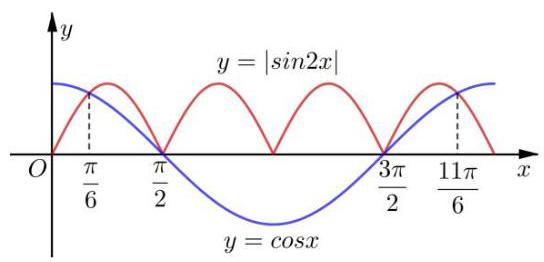
\includegraphics[max width=0.4\textwidth]{images/bo_d7fhnv491nqc73ercsbg_72_240_854_544_262_0.jpg}
\end{center}
\hspace*{3em} 

因为 \(0 < \frac{\pi }{6} < 1,5 < \frac{11\pi }{6} < 6\) ,所以满足条件的正整数有 \(1\text{ 、 }2\text{ 、 }3\text{ 、 }4\text{ 、 }5\) 共五个,故选 C.

12.(2025 高三二模奉贤 16)若 \({5\pi }\) 是函数 \(y = \cos {nx}\sin \frac{2000}{{n}^{2}}x\) 的一个周期，则正整数 \(n\) 所有可能取值个数是( )

A. 2 B. 3 C. 4 D. 9

【答案】B

【解析】利用周期定义 \(f\left( {x + {5\pi }}\right)  = f\left( x\right)\) ,由

\(\cos \left( {{nx} + {5n\pi }}\right) \sin \left( {\frac{2000}{{n}^{2}}x + \frac{10000\pi }{{n}^{2}}}\right)  = \cos {nx}\sin \frac{2000}{{n}^{2}}x,\)

得 \({\left( -1\right) }^{5n} = 1\) ( \(n\) 为偶数) 且 \(\frac{10000\pi }{{n}^{2}} = {2k\pi }\) ( \(k\) 为整数),即 \({n}^{2}\) 整除 5000 ,

设 \(n = {2m}\) ,则 \(4{m}^{2}\) 整除 5000,即 \({m}^{2}\) 整除 \({1250} = 2 \times  {5}^{4}\) ,分析 1250 的因数, \(m = 1,5,{25}\) , 对应 \(n = 2,{10},{50}\) ,

当 \(n = 2\) 时, \(y = \cos {2x}\sin {500x},{5\pi }\) 是周期;

当 \(n = {10}\) 时, \(y = \cos {10x}\sin {20x},{5\pi }\) 是周期;

当 \(n = {50}\) 时, \(y = \cos {50x}\sin {0.8x},{5\pi }\) 是周期;

故选 B.

13.(2025 高三二模长宁 17)已知向量 \(\overrightarrow{m} = \left( {\sin x + \cos x,2\sin x}\right) ,\overrightarrow{n} = \left( {\sin x - \cos x,\sqrt{3}\cos x}\right)\) ， \(f\left( x\right)  = \overrightarrow{m} \cdot  \overrightarrow{n}.\)

(1)求函数 \(y = f\left( x\right)\) 的单调递减区间；

(2)若函数 \(y = f\left( x\right)  - a\) 在区间 \(\left( {0,\frac{\pi }{2}}\right)\) 上恰有 2 个零点，求实数 \(a\) 的取值范围.

【答案】(1) \(\left\lbrack  {\frac{\pi }{3} + {k\pi },\frac{5\pi }{6} + {k\pi }}\right\rbrack  \left( {k \in  \mathbf{Z}}\right)\) ; (2) \(1 < a < 2\)

【解析】(1) \(f\left( x\right)  =  - \cos {2x} + \sqrt{3}\sin {2x} = 2\sin \left( {{2x} - \frac{\pi }{6}}\right)\) , .3 分因为 \(y = f\left( x\right)\) 单调递减,所以 \(\frac{\pi }{2} + {2k\pi } \leq  {2x} - \frac{\pi }{6} \leq  \frac{3\pi }{2} + {2k\pi }\) , .1 分即: \(\frac{\pi }{3} + {k\pi } \leq  x \leq  \frac{5\pi }{6} + {k\pi }\) ,

所以 \(y = f\left( x\right)\) 的单调递减得单调递减区间是 \(\left\lbrack  {\frac{\pi }{3} + {k\pi },\frac{5\pi }{6} + {k\pi }}\right\rbrack  \left( {k \in  \mathbf{Z}}\right)\) ; .2 分

(2)函数 \(y = f\left( x\right)  - a\) 在区间 \(\left( {0,\frac{\pi }{2}}\right)\) 上恰有 2 个零点，即 \(2\sin \left( {{2x} - \frac{\pi }{6}}\right)  = a\) 在 \(\left( {0,\frac{\pi }{2}}\right)\) 上恰有两个解,令 \(t = {2x} - \frac{\pi }{6},t \in  \left( {-\frac{\pi }{6},\frac{5\pi }{6}}\right)\) ,

所以 \(2\sin t = a\) 在 \(\left( {-\frac{\pi }{6},\frac{5\pi }{6}}\right)\) 上恰有两个解, .2 分

当 \(t \in  \left( {-\frac{\pi }{6},\frac{\pi }{2}}\right)\) 时,函数 \(y = 2\sin t\) 单调递增,且 \(\sin t \in  ( - 1,2\rbrack\) , .2 分

当 \(t \in  \left\lbrack  {\frac{\pi }{2},\frac{5\pi }{6}}\right)\) 时,函数 \(y = 2\sin t\) 单调递减,且 \(\sin t \in  (1,2\rbrack\) , .2 分

所以当 \(1 < a < 2\) 时,函数 \(y = f\left( x\right)  - a\) 在区间 \(\left( {0,\frac{\pi }{2}}\right)\) 上恰有 2 个零点. .2 分

14.(2025 高三二模静安 17)已知向量 \(\overrightarrow{a} = \left( {\cos \left( {x + \frac{\pi }{6}}\right) ,\sin \left( {x + \frac{\pi }{6}}\right) }\right)\) 、 \(\overrightarrow{b} = \left( {\cos \left( {x + \frac{\pi }{6}}\right) , - \sin \left( {x + \frac{\pi }{6}}\right) }\right)\) ,记 \(f\left( x\right)  = \overrightarrow{a} \cdot  \overrightarrow{b}\) .

(1)求函数 \(y = f\left( x\right)\) 的最小正周期；

(2)若函数 \(y = f\left( {x + \theta }\right)\) (其中常数 \(\theta  \in  \left( {0,\frac{\pi }{2}}\right)\) )为奇函数，求 \(\theta\) 的值.

【答案】(1) \(\pi ;\left( 2\right) \theta  = \frac{\pi }{12}\)

【解析】(1) \(f\left( x\right)  = \overrightarrow{a} \cdot  \overrightarrow{b} = \cos \left( {{2x} + \frac{\pi }{3}}\right)\) ,(4 分)

故,函数 \(y = f\left( x\right)\) 的最小正周期为 \(\frac{2\pi }{2} = \pi\) . (2 分)

(2) \(f\left( {x + \theta }\right)  = \cos \left( {{2x} + {2\theta } + \frac{\pi }{3}}\right)\) .(2 分)

由函数 \(y = f\left( {x + \theta }\right)\) 为奇函数,得 \(f\left( {0 + \theta }\right)  = 0\) (此处也可以用诱导公式推得)

即 \({2\theta } + \frac{\pi }{3} = {k\pi } + \frac{\pi }{2},\theta  = \frac{k\pi }{2} + \frac{\pi }{12},k \in  \mathbf{Z}\) ,(4 分) 由常数 \(\theta  \in  \left( {0,\frac{\pi }{2}}\right)\) ,解得 \(\theta  = \frac{\pi }{12}\) . (2 分)

15. (2025 高三二模普陀 18)设 \(\omega  > 0\) ，函数 \(y = f\left( x\right)\) 的表达式为 \(f\left( x\right)  = \cos \left( {{\omega x} - \frac{\pi }{6}}\right)\) .

(1)若 \(\omega  = 2\) ，设 \(\bigtriangleup  {ABC}\) 的内角 \(A\) ， \(B\) ， \(C\) 的对边分别为 \(a\) ， \(b\) ， \(c\) ， \(f\left( C\right)  =  - \frac{\sqrt{3}}{2}\) ， 且 \({c}^{2} - {a}^{2} - {b}^{2} = 4\) ,求 \(\bigtriangleup {ABC}\) 的面积.

(2)对任意的 \({x}_{0} \in  \mathbf{R}\) ，皆有 \(f\left( {x}_{0}\right)  \leq  f\left( \frac{\pi }{3}\right)\) 成立，且该函数在区间 \(\left( {\frac{\pi }{6},\frac{\pi }{2}}\right)\) 上不存在最小值,求函数 \(y = f\left( x\right)\) 在 \(x \in  \left( {\frac{4\pi }{3},\frac{17\pi }{6}}\right)\) 的单调区间.

【答案】(1) \(\sqrt{3}\) ；(2)单调增区间是 \(\left| {\frac{7\pi }{3},\frac{17\pi }{6}}\right|\) ，单调减区间是 \(\left| {\frac{4\pi }{3},\frac{7\pi }{3}}\right|\)

【解析】(1) 由 \(\cos \left| {{2C} - \frac{\pi }{6}}\right|  =  - \frac{\sqrt{3}}{2}\) 且 \(C \in  \left( {0,\pi }\right)\) ,得

\(C = \frac{\pi }{2}\) 或 \(C = \frac{2\pi }{3},\) .2 分

当 \(C = \frac{\pi }{2}\) 时,与 \({c}^{2} - {a}^{2} - {b}^{2} = 4\) 矛盾,不符合条件;

当 \(C = \frac{2\pi }{3}\) 时,则 \(\cos C = \frac{{a}^{2} + {b}^{2} - {c}^{2}}{2ab} = \frac{-4}{2ab} =  - \frac{1}{2}\) ,即 \({ab} = 4\) .4 分

则 \({S}_{\bigtriangleup {ABC}} = \frac{1}{2}{ab}\sin C = \frac{1}{2}4\frac{\sqrt{3}}{2} = \sqrt{3}\) . 6 分

(2)由条件得, \(\omega  \times  \frac{\pi }{3} - \frac{\pi }{6} = {2k\pi }\) ， \(k \in  \mathbf{Z}\) ，且 \(\frac{1}{2}T = \frac{2\pi }{2\omega } \geq  \frac{\pi }{6}\) ，

则 \(\omega  = \frac{1}{2}\) ,即 \(f\left( x\right)  = \cos \left| {\frac{1}{2}x - \frac{\pi }{6}}\right|\) , .4 分

当 \(x \in  \left| {\frac{4\pi }{3},\frac{17\pi }{6}}\right|\) 时,则 \(\frac{1}{2}x - \frac{\pi }{6} \in  \left| {\frac{\pi }{2},\frac{5\pi }{4}}\right|\) , .6 分

若 \(\frac{1}{2}x - \frac{\pi }{6} \in  \left| {\frac{\pi }{2},\pi }\right|\) ,即 \(x \in  \left| {\frac{4\pi }{3},\frac{7\pi }{3}}\right|\) 时,函数 \(y = f\left( x\right)\) 是严格减函数;

若 \(\frac{1}{2}x - \frac{\pi }{6} \in  \left| {\pi ,\frac{5\pi }{4}}\right|\) ,即 \(x \in  \left| {\frac{7\pi }{3},\frac{17\pi }{6}}\right|\) 时,函数 \(y = f\left( x\right)\) 是严格增函数,

则函数 \(y = f\left( x\right)\) 的单调增区间是 \(\left| {\frac{7\pi }{3},\frac{17\pi }{6}}\right|\) ,单调减区间是 \(\left| {\frac{4\pi }{3},\frac{7\pi }{3}}\right|\) . 8 分

16.(2025 高三二模闵行 18)已知 \(f\left( x\right)  = \sin \left( {{\omega x} + \varphi }\right) \left( {\omega  > 0,0 < \varphi  < \pi }\right)\) ，函数 \(y = f\left( x\right)\) 的部分图像如图所示,图中最高点 \(S\left( {\frac{\pi }{3},1}\right)\) ,最低点 \(T\left( {\frac{4\pi }{3}, - 1}\right)\)

\begin{center}
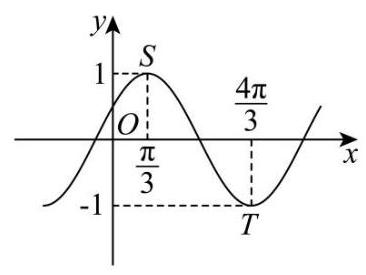
\includegraphics[max width=0.3\textwidth]{images/bo_d7fhnv491nqc73ercsbg_75_1045_1633_366_275_0.jpg}
\end{center}
\hspace*{3em} 

(1)求函数 \(y = f\left( x\right)\) 的解析式;

(2)若 \(\bigtriangleup {ABC}\) 的内角 \(A\text{ 、 }B\text{ 、 }C\) 所对的边分别为 \(a\text{ 、 }b\text{ 、 }c\) ， 若 \(A \neq  B,f\left( A\right)  = f\left( B\right) ,c = 2\) ,求 \(\bigtriangleup {ABC}\) 面积的取值范围.

【答案】( 1 ) \(f\left( x\right)  = \sin \left( {x + \frac{\pi }{6}}\right)\) ；( 2 ) \(\left( {0,\sqrt{3}}\right)\)

【解析】(1) 由图,因为 \(\frac{4\pi }{3} - \frac{\pi }{3} = \frac{T}{2}\) 得周期 \(T = {2\pi }\) ,由 \(\frac{2\pi }{\omega } = {2\pi }\) 得 \(\omega  = 1\) . 3 分又 \(f\left( \frac{\pi }{3}\right)  = 1\) 得 \(\frac{\pi }{3} + \varphi  = {2k\pi } + \frac{\pi }{2},k \in  \mathbf{Z}\) ,又因为 \(0 < \varphi  < \pi\) ,

所以 \(\varphi  = \frac{\pi }{6}\) ,所以 \(f\left( x\right)  = \sin \left( {x + \frac{\pi }{6}}\right)\) , .6 分

(2)因为 \(f\left( A\right)  = f\left( B\right)\) ，又 \(0 < A + B < \pi\) ， \(A \neq  B\) ，

结合图像可知: \(A + B = \frac{2}{3}\pi\) ， \(C = \frac{\pi }{3}\) ， .8 分

又 \(c = 2\) ,由余弦定理可得 \({c}^{2} = {a}^{2} + {b}^{2} - {2ab}\cos C = 4\) ,

所以 \({a}^{2} + {b}^{2} - 4 = {ab} \geq  {2ab} - 4\) ,所以 \(0 < {ab} \leq  4\) , 12 分

因为 \(A \neq  B\) ,所以 \(a \neq  b\) ,因此上述不等式中等号不能取到,

所以 \(S = \frac{1}{2}{ab}\sin C \in  \left( {0,\sqrt{3}}\right)\) ，因此， \(\bigtriangleup {ABC}\) 面积 \(S\) 的取值范围为 \(\left( {0,\sqrt{3}}\right)\) . . . . . .14 14 分

\section*{五、三角应用题}

1.(2025 高三二模松江 8)在定向越野活动中，测得甲在乙北偏东 \({80}^{ \circ  }\) 的方向，甲乙两人间的距离为 \(2\mathrm{\;{km}}\) ,丙在乙北偏西 \({40}^{ \circ  }\) 的方向,甲丙两人间的距离为 \(\sqrt{7}\mathrm{\;{km}}\) ,则乙丙两人间的距离为\_\_\_\_\_km.

【答案】 1

【解析】设甲为 \(A\) 点，乙为 \(B\) 点，丙为 \(C\) 点，可构成 \(\bigtriangleup  {ABC}\) ，由题意可得 \({AB} = 2\) ，

\({AC} = \sqrt{7},\angle {ABC} = {80}^{ \circ  } + {40}^{ \circ  } = {120}^{ \circ  }\) ,

由余弦定理可得 \(A{C}^{2} = B{A}^{2} + B{C}^{2} - {2BA} \cdot  {BC} \cdot  \cos \angle {ABC}\) ,

解得 \({BC} = 1\) 或 \({BC} =  - 3\) (舍)，所以乙丙两人间的距离为 \(1\mathrm{\;{km}}\) .

2.(2025 高三二模静安 8)设某港口水的深度 \(y\) (米)关于时间 \(t\) (时)的函数近似满足 \(y = h + A\sin \left( {{\omega t} + \phi }\right)\) . 根据某一天的测量,港口水的深度在早上 3 点达到最大值 18 米,之后持续减少，并在上午 9 点达到最小值 14 米. 则该港口水的深度 \(y\) (米)关于时间 \(t\) (时) 的函数的近似表达式为\_\_\_\_\_.

【答案】 \(y = {16} + 2\sin \left( {\frac{\pi }{6}t}\right)\)

【解析】由题意知 \(\frac{1}{2}T = 6 \Rightarrow  T = {12} = \frac{2\pi }{\omega } \Rightarrow  \omega  = \frac{\pi }{6}\) ,又 \(\left\{  {\begin{array}{l} h + A = {18} \\  h - A = {14} \end{array} \Rightarrow  \left\{  \begin{array}{l} h = {16} \\  A = 2 \end{array}\right. }\right.\) , \(\therefore y = {16} + 2\sin \left( {\frac{\pi }{6}t + \phi }\right)\) ,将点 \(\left( {3,{18}}\right)\) 代入,解得 \(\phi  = 0,\therefore y = {16} + 2\sin \left( {\frac{\pi }{6}t}\right)\) .

\begin{center}
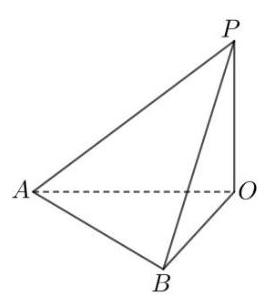
\includegraphics[max width=0.2\textwidth]{images/bo_d7fhnv491nqc73ercsbg_77_1245_218_264_301_0.jpg}
\end{center}
\hspace*{3em} 

3.(2025 高三二模浦东 10)如图，某建筑物 \({OP}\) 垂直于地面，从地面点 \(A\) 处测得建筑物顶部 \(P\) 的仰角为 \({30}^{ \circ  }\) ，从地面点 \(B\) 处测得建筑物顶部 \(P\) 的仰角为 \({45}^{ \circ  }\) ,已知 \(A,B\) 相距 100 米, \(\angle {AOB} = {60}^{ \circ  }\) ,则该建筑物 \({OP}\) 的高度约为\_\_\_\_\_米.(保留一位小数)

【答案】66.4

【解析】设 \({PO} = x\) ,由题意可得 \({OA} = \sqrt{3}x,{OB} = x\) ,在 \(\bigtriangleup {AOB}\) 中, 由余弦定理可得 \(A{B}^{2} = O{A}^{2} + O{B}^{2} - {2OA} \cdot  {OB} \cdot  \cos \angle {AOB}\) , \({100}^{2} = 3{x}^{2} + {x}^{2} - 2 \cdot  \sqrt{3}x \cdot  x \cdot  \cos {60}^{ \circ  }\) ,解得 \(x \approx  {66.4}\) ,

所以该建筑物 \({OP}\) 的高度约为 66.4 米.

4.(2025 高三二模金山 11)如图，现对某景区一长 \({AB} = {600}\mathrm{\;m}\) ，宽 \({AD} = {360}\mathrm{\;m}\) 的矩形空地进行建设. 规划在边 \({AB}\text{ 、 }{AD}\) 上分别取点 \(M\) 、 \(N\) 修建人行步道 (不考虑宽度),且满足点 \(A\) 关于步道 \({MN}\) 的对称点 \(E\) 在边 \({DC}\) 上. 在 \(\bigtriangleup {AMN}\) 内种植花卉,在 \(\bigtriangleup {EMN}\) 内搭建娱乐设施,其余区域规划为露营区，则人行步道 \({MN}\) 的最短距离为\_\_\_\_\_m. (结果精确到 1m)

\begin{center}
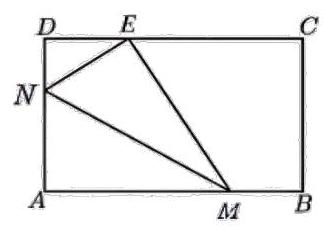
\includegraphics[max width=0.2\textwidth]{images/bo_d7fhnv491nqc73ercsbg_77_1203_798_323_228_0.jpg}
\end{center}
\hspace*{3em} 

第 11 题 图

【答案】468

【解析】设 \(\angle {AMN} = \alpha\) ，则 \(\sin \alpha  = \frac{AN}{MN} \Rightarrow  {AN} = {MN}\sin \alpha\) ，

因为点 \(A\) 关于步道 \({MN}\) 的对称点 \(E\) 在边 \({CD}\) 上,则

\(\angle {EMN} = \alpha ,{AN} = {NE} \Rightarrow  \angle {END} = {2\alpha } \Rightarrow  \cos {2\alpha } = \frac{DN}{NE} \Rightarrow  {DN} = {NE}\cos {2\alpha }\) ,

\(\therefore {DN} = {AN}\cos {2\alpha } = {MN}\sin \alpha \cos {2\alpha }\) ,

\(\because {AD} = {DN} + {AN} = {360},\therefore {MN}\sin \alpha \cos {2\alpha } + {MN}\sin \alpha  = {360}\) ,

\(\therefore {MN} = \frac{360}{\sin \alpha \cos {2\alpha } + \sin \alpha } = \frac{360}{\sin \alpha \left( {1 - 2{\sin }^{2}\alpha }\right)  + \sin \alpha }\)

\(= \frac{360}{2\sin \alpha  - 2{\sin }^{3}\alpha } = \frac{180}{\sin \alpha  - {\sin }^{3}\alpha },\)

因为要求 \({MN}\) 的最小值,则只需求 \(f\left( \alpha \right)  = \sin \alpha  - {\sin }^{3}\alpha ,\left( {\sin \alpha  \in  \left( {0,1}\right) }\right)\) 的最大值即可, \({f}^{\prime }\left( \alpha \right)  = \cos \alpha  - 3{\sin }^{2}\alpha \cos \alpha  = \cos \alpha \left( {1 - 3{\sin }^{2}\alpha }\right) ,\)

当 \(\sin \alpha  \in  \left( {0,\frac{\sqrt{3}}{3}}\right)\) 时 \(f\left( \alpha \right)\) 单调递增,当 \(\sin \alpha  \in  \left( {\frac{\sqrt{3}}{3},1}\right)\) 时 \(f\left( \alpha \right)\) 单调递减,

则当 \(\sin \alpha  = \frac{\sqrt{3}}{3}\) 时, \(f{\left( \alpha \right) }_{\max } = \frac{2\sqrt{3}}{9}\) ,

则 \({MN}\) 的最短距离为 \(\frac{180}{\frac{2\sqrt{3}}{9}} \approx  {468}\) .

5.(2025 高三二模徐汇 11)如图，某处有一块圆心角为 \(\frac{2}{3}\pi\) 的扇形绿地 \({AOB}\) ,扇形的半径为 20 米, \({AB}\) 是一条原有的人行直路,由于工程建设需要,现要在绿地中建一条直路 \({OC}\) ,以便在图中阴影部分区域分类堆放物料. 为了尽量减少对绿地的破坏(不计路宽)，则原直路 \({AB}\) 与新直路 \({OC}\) 的交叉点 \(D\) 到 \(O\) 的距离为\_\_\_\_\_米.

\begin{center}
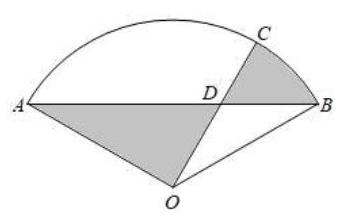
\includegraphics[max width=0.2\textwidth]{images/bo_d7fhnv491nqc73ercsbg_78_1179_526_340_219_0.jpg}
\end{center}
\hspace*{3em} 

【答案】 \({10}\sqrt{2}\)

【解析】作 \({AE} \bot  {AB}\) 交 \({AB}\) 于 \(E\) ,

\(\because {OA} = {20},\angle {AOB} = \frac{2\pi }{3},\therefore \angle {AOE} = \frac{\pi }{3},\therefore {OE} = {20}\cos \frac{\pi }{3} = {10}\) ,

设 \(\angle {BOD} = \alpha ,\therefore \angle {DOE} = \frac{\pi }{3} - \theta ,\cos \left( {\frac{\pi }{3} - \theta }\right)  = \frac{10}{OD},\therefore {OD} = \frac{10}{\cos \left( {\frac{\pi }{3} - \theta }\right) }\) ,

\(\therefore S = {S}_{\bigtriangleup {AOD}} + {S}_{\text{ 扇形 }{BOC}} - {S}_{\bigtriangleup {BOD}} = \frac{1}{2} \times  {20} \times  \frac{10}{\cos \left( {\frac{\pi }{3} - \theta }\right) } \times  \sin \left( {\frac{2\pi }{3}\theta }\right)\)

\(+ \frac{1}{2} \times  {20} \times  {20} \times  \theta  - \frac{1}{2} \times  {20} \times  \frac{10}{\cos \left( {\frac{\pi }{3} - \theta }\right) } \times  \sin \theta  = \frac{100}{\cos \left( {\frac{\pi }{3} - \theta }\right) }\left\lbrack  {\sin \left( {\frac{2\pi }{3}\theta }\right)  - \sin \theta }\right\rbrack   + {200\theta }\)

\(= \frac{100}{\cos \left( {\frac{\pi }{3} - \theta }\right) } \cdot  \sin \left( {\frac{\pi }{3} - \theta }\right)  + {200\theta }\left( {\theta  \in  \left\lbrack  {0,\frac{\pi }{2}}\right\rbrack  }\right) ,\)

\(\therefore {S}^{\prime } = {100}\left( \frac{-{\cos }^{2}\left( {\frac{\pi }{3} - \theta }\right)  - {\sin }^{2}\left( {\frac{\pi }{3} - \theta }\right) }{{\cos }^{2}\left( {\frac{\pi }{3} - \theta }\right) }\right)  + {200} = \frac{-{100}}{{\cos }^{2}\left( {\frac{\pi }{3} - \theta }\right) } + {200}\) ,

\begin{center}
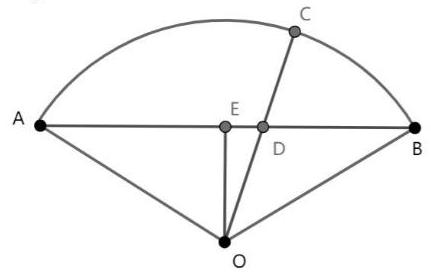
\includegraphics[max width=0.3\textwidth]{images/bo_d7fhnv491nqc73ercsbg_78_1051_1868_431_278_0.jpg}
\end{center}
\hspace*{3em} 

\({S}^{\prime } = 0 \Rightarrow  \cos \left( {\frac{\pi }{3} - \theta }\right)  = \frac{\sqrt{2}}{2},\)

可得此时取得面积的最小值,此时 \({OD} = {10} \div  \frac{\sqrt{2}}{2} = {10}\sqrt{2}\) .

6.(2025 高三二模奉贤 11)中企联合大厦是奉贤区的第一高楼,是奉贤美奉贤强的一个缩影.

某数学建模兴趣小组的同学们去实地进行测量，经过多次的测量，最终在平行于地面的同

一水平面上选取三个点: 点 \(B\) 、点 \(C\) 、点 \(O\) 作为测量基点. 设大厦的最高点为 \(A\) ,在点 \(B\) 处测得点 \(A\) 的仰角为 \(\angle {ABO} = \theta  = {71.5}^{ \circ  }\) ，在点 \(C\) 处测得点 \(A\) 的仰角为 \(\angle {ACO} = {44}^{ \circ  }\) ，又测得 \({BC} = {221}\) 米， \(\angle {BOC} = {119}^{ \circ  }\) ，(见图).

\begin{center}
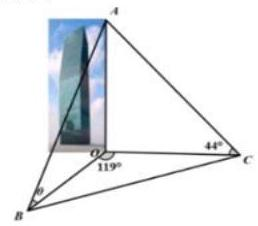
\includegraphics[max width=0.2\textwidth]{images/bo_d7fhnv491nqc73ercsbg_79_1324_356_258_226_0.jpg}
\end{center}
\hspace*{3em} 

第 11 题图

现作出以下几个假设:

 \circled{1}  直线 \({AO}\) 垂直于平面 \({OBC}\) ；

 \circled{2} 平面 \({OBC}\) 到地面的距离等于测角仪高度，在计算过程中测角仪高度忽略不计；  \circled{3} 其它次要因素等忽略不计.

根据以上信息估算奉贤第一高楼的高度约\_\_\_\_\_米. (结果保留整数)

【答案】 179

【解析】在 \(\bigtriangleup {ABO}\) 中, \(\tan {71.5}^{ \circ  } = \frac{OA}{OB} \Rightarrow  {OB} = \frac{OA}{\tan {71.5}^{ \circ  }}\) ,

在 \(\bigtriangleup {ACO}\) 中, \(\tan {44}^{ \circ  } = \frac{OA}{OC} \Rightarrow  {OC} = \frac{OA}{\tan {44}^{ \circ  }}\) ,

在 \(\bigtriangleup {BCO}\) 中,

\(B{C}^{2} = O{B}^{2} + O{C}^{2} - {2OB} \cdot  {OC} \cdot  \cos {119}^{ \circ  }\)

\(\Rightarrow  {221}^{2} = {\left( \frac{OA}{\tan {71.5}^{ \circ  }}\right) }^{2} + {\left( \frac{OA}{\tan {44}^{ \circ  }}\right) }^{2} - 2 \times  \frac{OA}{\tan {71.5}^{ \circ  }} \times  \frac{OA}{\tan {44}^{ \circ  }} \times  \cos {119}^{ \circ  }\) ,

\(\therefore {OA} \approx  {179}\) .

\section*{第四部分 数列}

\section*{一、等差数列与等比数列的性质及其运用}

1.(2025 高三二模奉贤 1)等差数列首项为 1 ，公差是 3 ，则第 5 项等于\_\_\_\_\_.

【答案】 13

【解析】 \({a}_{5} = 1 + 4 \times  3 = {13}\) .

2.(2025 高三二模黄浦 7)已知等比数列 \(\left\{  {a}_{n}\right\}\) 为严格增数列，其前 \(n\) 项和为 \({S}_{n}\) ，若 \({a}_{1}{a}_{10} = {a}_{8}\) ， \({S}_{4} - {S}_{1} = \frac{21}{4}\) ，则该数列的公比为\_\_\_\_\_.

【答案】 4

【解析】由 \({a}_{1}{a}_{10} = {a}_{8}\) 可得 \({a}_{1}^{2}{q}^{9} = {a}_{1}{q}^{7} \Rightarrow  {a}_{1}{q}^{2} = 1\) ,即 \({a}_{3} = 1\) ,

\({S}_{4} - {S}_{1} = {a}_{4} + {a}_{3} + {a}_{2} = {a}_{3}q + {a}_{3} + \frac{{a}_{3}}{q} = \frac{21}{4}\) ,化简可得 \(4{q}^{2} - {17q} + 4 = 0\) ,

解得 \(q = 4\) 或 \(q = \frac{1}{4}\) ,又因为数列 \(\left\{  {a}_{n}\right\}\) 为严格增数列,所以 \(q = 4\) .

3. (2025 高三二模金山 8)已知 \(\left\{  {a}_{n}\right\}\) 是等差数列，若 \({a}_{3}\text{ 、 }{a}_{7}\) 分别是函数 \(y = {x}^{2} - {4x} + 2\) 的两个零点,则 \({a}_{5} =\) \_\_\_\_\_.

【答案】 2

【解析】由题意可知 \({a}_{3} + {a}_{7} = 2{a}_{5} = 4 \Rightarrow  {a}_{5} = 2\) .

4.(2025 高三二模闵行 10)已知数列 \(\left\{  {a}_{n}\right\}\) 为等差数列，数列 \(\left\{  {b}_{n}\right\}\) 为等比数列，且 \({a}_{1} = {b}_{1} = 1\) ， \({a}_{2} = {b}_{2} = t\) ，若 \({a}_{6} + {b}_{6} > {38}\) ，则实数 \(t\) 的取值范围为\_\_\_\_\_.

【答案】 \(\left( {2, + \infty }\right)\)

【解析】由题意知 \({a}_{n} = 1 + \left( {n - 1}\right) \left( {t - 1}\right) ,{b}_{n} = 1 \cdot  {t}^{n - 1}\) ,

则 \(\because {a}_{6} + {b}_{6} > {38},\therefore 1 + 5\left( {t - 1}\right)  + {t}^{5} > {38} \Rightarrow  {t}^{5} + {5t} > {42}\) ,

因为 \(f\left( t\right)  = {t}^{5} + {5t}\) 单调递增,且 \(f\left( 2\right)  = {42} \Rightarrow  t > 2\) .

5.(2025 高三二模崇明 16)数列 \(\left\{  {a}_{n}\right\}\) 是等差数列，周期数列 \(\left\{  {b}_{n}\right\}\) 满足 \({b}_{n} = \cos \left( {a}_{n}\right)\) ，若集合 \(X = \left\{  {x \mid  x = {b}_{n},n}\right.\) 是正整数 \(\}\) 中恰有三个元素,则数列 \(\left\{  {b}_{n}\right\}\) 的周期 \(T\) 的取值不可能是 ( )

A. 4 B. 5 C. 6 D. 7

【答案】D

【解析】 \circled{1}  \({a}_{n} = \frac{n\pi }{2},{b}_{n} = \cos \frac{n\pi }{2},X = \{ 0, - 1,1\} ,T = 4\) ，则 \(\mathrm{A}\) 可能；

 \circled{2}  \({a}_{n} = \frac{2n\pi }{5},{b}_{n} = \cos \frac{2n\pi }{5},X = \left\{  {\frac{\sqrt{5} - 1}{4}, - \frac{\sqrt{5} + 1}{4},1}\right\}  ,T = 5\) ，则 \(\mathrm{B}\) 可能；

 \circled{3}  \({a}_{n} = \frac{n\pi }{3} - \frac{\pi }{6},{b}_{n} = \cos \left( {\frac{n\pi }{3} - \frac{\pi }{6}}\right) ,X = \left\{  {\frac{\sqrt{3}}{2}, - \frac{\sqrt{3}}{2},0}\right\}  ,T = 6\) ，则 \(\mathrm{C}\) 可能；

故选 D.

又解: 考虑一个单位圆的内接正多边形, 正多边形各个顶点的横坐标只有三个不同的取值, 则正多边形可能是正方形, 正五边形, 正六边形, 不可能是正七边形, 故选 D.

6. (2025 高三二模杨浦 16)设 \(A\) 是由 \(k\) 个二次函数组成的集合，对于连续的正整数 \(1,2,3,\ldots ,{2025}\) ,存在二次函数 \(y = {f}_{i}\left( x\right)  \in  A,\left( {1 \leq  i \leq  {2025},i \in  \mathbf{Z},y = {f}_{i}\left( x\right) \text{ 可重复),使得 }}\right) \; {f}_{1}\left( 1\right) ,{f}_{2}\left( 2\right) ,{f}_{3}\left( 3\right) ,\ldots ,{f}_{2025}\left( {2025}\right)\) 是等差数列,则 \(k\) 的最小可能值是 ( )

A. 507 B. 1013 C. 1519 D. 2025

【答案】B

【解析】等差数列 \({a}_{n} = {a}_{1} + \left( {n - 1}\right) d = {dn} + \left( {{a}_{1} - d}\right)\) ,是关于 \(n\) 的一次函数,所以点 \(\left( {1,{f}_{1}\left( 1\right) }\right) ,\left( {2,{f}_{2}\left( 2\right) }\right) ,\cdots ,\left( {{2025},{f}_{1}\left( {2025}\right) }\right)\) 在一条直线上,而方程 \({f}_{k}\left( n\right)  = {dn} + \left( {{a}_{1} - d}\right)\) 最多有 2 个解, 因此每个二次函数最多包含等差数列中的 2 个值, 因为 \({2025} \div  2 = {1012}\cdots \cdots 1\) ,至少需 \({1012} + 1 = {1013}\) 个二次函数,故 \(k\) 的最小值为 1013,

例如: 取 \({f}_{{2i} - 1}\left( x\right)\) 和 \({f}_{2i}\left( x\right)\) 为 \(y = \left( {x - {2i} + 1}\right) \left( {x - {2i}}\right) ,1 \leq  i \leq  {1012},i \in  \mathbf{Z}\) , \({f}_{2025}\left( x\right)  = {\left( x - {2025}\right) }^{2}\) ,则 \({f}_{1}\left( 1\right) ,{f}_{2}\left( 2\right) ,{f}_{3}\left( 3\right) ,\ldots ,{f}_{2025}\left( {2025}\right)\) 是常数列,为等差数列, 故选 B.

\section*{二、数列求通项、求和}

1. (2025 高三二模长宁 3)已知数列 \(\left\{  {a}_{n}\right\}\) 是等差数列，且 \({a}_{1} = 2,{a}_{6} = {17}\) ，则其前 7 项和 \({S}_{7} =\) \_\_\_\_\_.

【答案】 77

【解析】 \({a}_{6} = {a}_{1} + {5d} \Rightarrow  d = 3\) ,所以 \({a}_{7} = {a}_{6} + d = {20}\) ,所以 \({S}_{7} = \frac{7\left( {{a}_{1} + {a}_{7}}\right) }{2} = {77}\) .

2.(2025 高三二模嘉定 4)已知等比数列 \(\left\{  {a}_{n}\right\}\) 的首项为 1，公比为 \(q\) ，其前 \(n\) 项和为 \({S}_{n}\) ，若 \({S}_{2} > {S}_{4}\) ，则 \(q\) 的取值范围为\_\_\_\_\_.

【答案】 \(\left( {-\infty , - 1}\right)\)

【解析】若 \({S}_{2} > {S}_{4}\) ,则 \(\frac{{a}_{1}\left( {1 - {q}^{2}}\right) }{1 - q} > \frac{{a}_{1}\left( {1 - {q}^{4}}\right) }{1 - q}\) ,化简可得 \(- {q}^{2}\left( {1 + q}\right)  > 0\) , 解得 \(q \in  \left( {-\infty , - 1}\right)\) .

3.(2025 高三二模普陀4)设 \(n \geq  1\) ， \(n \in  \mathbf{N}\) ， \({S}_{n}\) 是等差数列 \(\left\{  {a}_{n}\right\}\) 的前 \(n\) 项和，若 \({a}_{3n} = 3{a}_{n} \neq  0\) ， 则 \(\frac{{S}_{5}}{{a}_{10}}\) 的值为\_\_\_\_\_.

【答案】 \(\frac{3}{2}\)

【解析】由题意可得 \({a}_{1} + \left( {{3n} - 1}\right) d = 3\left\lbrack  {{a}_{1} + \left( {n - 1}\right) d}\right\rbrack   \Rightarrow  {a}_{1} = d\) , \({S}_{5} = 5{a}_{1} + \frac{5 \times  4}{2}d = {15d},\;{a}_{10} = {a}_{1} + \left( {{10} - 1}\right) d = {10d}\) ,所以 \(\frac{{S}_{5}}{{a}_{10}} = \frac{3}{2}\) .

4.(2025 高三二模浦东 6)若数列 \(\left\{  {a}_{n}\right\}\) 为等差数列，其前 \(n\) 项和为 \({S}_{n}\) ，已知 \({a}_{3} + {a}_{15} = 2\) ， 则 \({S}_{17} =\) \_\_\_\_\_.

【答案】 17

【解析】 \({S}_{17} = \frac{{17}\left( {{a}_{1} + {a}_{17}}\right) }{2} = \frac{{17}\left( {{a}_{3} + {a}_{15}}\right) }{2} = \frac{{17} \times  2}{2} = {17}\) .

5.(2025 高三二模青浦 7)已知数列 \(\left\{  {a}_{n}\right\}\) 满足 \({a}_{1} = 1,{a}_{n} = 2{a}_{n + 1}\) ，则 \(\mathop{\sum }\limits_{{i = 1}}^{{+\infty }}{a}_{i} =\) \_\_\_\_\_.

【答案】 2

【解析】由题意知是 \(\left\{  {a}_{n}\right\}\) 以 1 为首项, \(\frac{1}{2}\) 为公比的等比数列,则 \(\mathop{\sum }\limits_{{i = 1}}^{{+\infty }}{a}_{i} = \frac{1}{1 - \frac{1}{2}} = 2\) .

6.(2025 高三二模黄浦 11)设 \(\left\{  {a}_{n}\right\}\) 为等差数列，其前 \(n\) 项和为 \({S}_{n}\) ，若 \(\left( {{S}_{8} - {S}_{7}}\right) \left( {{S}_{9} - {S}_{7}}\right)  < 0\) ， 则满足 \({S}_{m}{S}_{m + 1} < 0\) 的正整数 \(m =\) \_\_\_\_\_.

【答案】 15

【解析】 \(\left( {{S}_{8} - {S}_{7}}\right) \left( {{S}_{9} - {S}_{7}}\right)  < 0\) ,即 \({a}_{8}\left( {{a}_{8} + {a}_{9}}\right)  < 0\) , 当 \({a}_{8} > 0\) 时, \({a}_{8} + {a}_{9} < 0\) ,

\({S}_{15} = \frac{{15}\left( {{a}_{1} + {a}_{15}}\right) }{2} = {15}{a}_{8} > 0,{S}_{16} = \frac{{16}\left( {{a}_{1} + {a}_{16}}\right) }{2} = 8\left( {{a}_{8} + {a}_{9}}\right)  < 0\) ,此时 \(m = {15}\) , 当 \({a}_{8} < 0\) 时， \({a}_{8} + {a}_{9} > 0\) ，

\({S}_{15} = \frac{{15}\left( {{a}_{1} + {a}_{15}}\right) }{2} = {15}{a}_{8} < 0,\;{S}_{16} = \frac{{16}\left( {{a}_{1} + {a}_{16}}\right) }{2} = 8\left( {{a}_{8} + {a}_{9}}\right)  > 0\) ,此时 \(m = {15}\) ,

综上,满足 \({S}_{m}{S}_{m + 1} < 0\) 的正整数 \(m = {15}\) .

7.(2025 高三二模杨浦 12)由若干个多边形所覆盖的区域，称为这些多边形的并集，例如图中,梯形 \({ACDE}\) 是 \(\bigtriangleup {ACE}\) 与矩形 \({BCDE}\) 的并集. 已知 \(n\) 是正整数,在平面直角坐标系 \({xOy}\) 中,直线 \({l}_{n}\) 的方程为 \(y =  - {2}^{n}x + n\) ,若直线 \({l}_{n}\) 交 \(x\) 轴于点 \({A}_{n}\) ,交 \(y\) 轴于点 \({B}_{n}\) ,则 \(\bigtriangleup  {A}_{1}O{B}_{1}\) 、 \(\bigtriangleup  {A}_{2}O{B}_{2}\) 、 \(\cdots\) 、 \(\bigtriangleup  {A}_{10}O{B}_{10}\) 的并集，其面积为\_\_\_\_\_.

\begin{center}
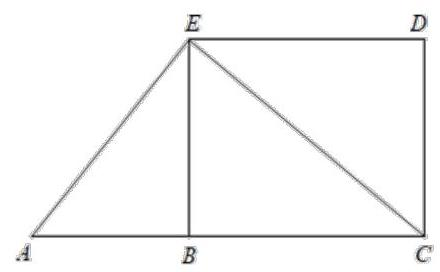
\includegraphics[max width=0.3\textwidth]{images/bo_d7fhnv491nqc73ercsbg_83_243_863_440_272_0.jpg}
\end{center}
\hspace*{3em} 

第 12 题图

【答案】 \(\frac{767}{1024}\)

【解析】由题意可得 \({A}_{n}\left( {\frac{n}{{2}^{n}},0}\right) ,{B}_{n}\left( {0,n}\right)\) ,

令 \({a}_{n} = \frac{n}{{2}^{n}}\) ,则 \({a}_{n + 1} - {a}_{n} = \frac{n + 1}{{2}^{n + 1}} - \frac{n}{{2}^{n}} = \frac{1 - n}{{2}^{n + 1}}\) ,

当 \(n = 1\) 时， \({a}_{n + 1} - {a}_{n} = 0\) ，当 \(n \geq  2\) 时， \({a}_{n + 1} - {a}_{n} < 0\) ，所以 \({a}_{1} = {a}_{2} > {a}_{3} > {a}_{4} > \cdots\) ， 随着三角形的个数增加, 所有三角形围成的图形每次增加一个小三角形,

设直线 \({l}_{n}\) 与 \({l}_{n + 1}\) 的交点为 \({C}_{n}\) ,

联立 \(\left\{  \begin{array}{l} y =  - {2}^{n}x + n \\  y =  - {2}^{n + 1}x + n + 1 \end{array}\right.\) ,解得 \(x = \frac{1}{{2}^{n}},y = n - 1\) ,即 \({C}_{n}\left( {\frac{1}{{2}^{n}},n - 1}\right)\) ,

则 \({S}_{\Delta {C}_{n}{B}_{a}{B}_{n + 1}} = \frac{1}{2}\left| {{B}_{n}{B}_{n + 1}}\right|  \cdot  {x}_{{C}_{n}} = \frac{1}{2} \times  \left( {n + 1 - n}\right)  \times  \frac{1}{{2}^{n}} = \frac{1}{{2}^{n + 1}}\)

设前 \(n\) 个三角形围成图形的面积为 \({S}_{n}\) ,则 \({S}_{n + 1} - {S}_{n} = {S}_{\Delta {C}_{n}{B}_{n}{B}_{n + 1}} = \frac{1}{{2}^{n + 1}}\) ,

且 \({S}_{1} = {S}_{{\Delta O}{A}_{1}{B}_{1}} = \frac{1}{2} \times  \frac{1}{2} \times  1 = \frac{1}{4}\) ,

则 \({S}_{2} - {S}_{1} = \frac{1}{{2}^{2}},{S}_{3} - {S}_{2} = \frac{1}{{2}^{3}},\ldots ,{S}_{n} - {S}_{n - 1} = \frac{1}{{2}^{n}},n \geq  2\) ,

由累加法可得 \({S}_{n} - {S}_{1} = \frac{1}{{2}^{2}} + \frac{1}{{2}^{3}} + \cdots  + \frac{1}{{2}^{n}} = \frac{\frac{1}{{2}^{2}} - \frac{1}{{2}^{n + 1}}}{1 - \frac{1}{2}} = \frac{1}{2} - \frac{1}{{2}^{n}}\left( {n \geq  2}\right)\) ,

则 \({S}_{n} = \frac{3}{4} - \frac{1}{{2}^{n}}\left( {n \geq  2}\right)\) ,当 \(n = 1\) 时, \({S}_{1} = \frac{1}{4}\) 符合通项,所以 \({S}_{n} = \frac{3}{4} - \frac{1}{{2}^{n}}\left( {n \geq  1,n \in  \mathbf{N}}\right)\) ,

所以 \({S}_{10} = \frac{3}{4} - \frac{1}{{2}^{10}} = \frac{767}{1024}\) ,即 \(\Delta {A}_{1}O{B}_{1}\text{ 、 }{A}_{2}O{B}_{2}\text{ 、 }\ldots \text{ 、 }\Delta {A}_{10}O{B}_{10}\) 的并集面积为 \(\frac{767}{1024}\) .

8.(2025高三二模嘉定)6)设数列 \(\left\{  {a}_{n}\right\}\) 满足 \({a}_{n} = \sin \left( \frac{n\pi }{3}\right)  + {\left( -1\right) }^{n}\cos \left( \frac{n\pi }{4}\right)\) ，记其前 \(n\) 项和为 \({S}_{n}\) ,前 \(n\) 项积为 \({T}_{n}\) . 则下列结论正确的是( )

A. 数列 \(\left\{  {S}_{n}\right\}\) 和数列 \(\left\{  {T}_{n}\right\}\) 均不是周期数列

B. 数列 \(\left\{  {S}_{n}\right\}\) 是周期数列,数列 \(\left\{  {T}_{n}\right\}\) 不是周期数列

C. 数列 \(\left\{  {S}_{n}\right\}\) 不是周期数列,数列 \(\left\{  {T}_{n}\right\}\) 是周期数列

D. 数列 \(\left\{  {S}_{n}\right\}\) 和数列 \(\left\{  {T}_{n}\right\}\) 均为周期数列

【答案】B

【解析】设 \({b}_{n} = \sin \left( \frac{n\pi }{3}\right) ,{c}_{n} = \cos \left( \frac{n\pi }{4}\right)  \cdot  {\left( -1\right) }^{n}\) ,

则 \({b}_{n + 6} = {b}_{n},{c}_{n + 8} = {c}_{n}\) ,所以 \({a}_{n + {24}} = {b}_{n + {24}} + {c}_{n + {24}} = {b}_{n} + {c}_{n} = {a}_{n}\) ,

由于 \({b}_{1} + {b}_{2} + {b}_{3} + {b}_{4} + {b}_{5} + {b}_{6} = 0,{c}_{1} + {c}_{2} + {c}_{3} + {c}_{4} + \cdots  + {c}_{8} = 0\) ,

所以 \({S}_{24} = 0\) ,所以 \({S}_{n + {24}} = {S}_{n}\) ,所以数列 \(\left\{  {S}_{n}\right\}\) 是周期数列;

\({a}_{1} = \frac{\sqrt{3}}{2} - \frac{\sqrt{2}}{2},{a}_{2} = \frac{\sqrt{3}}{2},{a}_{3} = \frac{\sqrt{2}}{2},{a}_{4} =  - \frac{\sqrt{3}}{2} - 1,{a}_{5} =  - \frac{\sqrt{3}}{2} + \frac{\sqrt{2}}{2},{a}_{6} = 0\) ,

可知 \({T}_{1},{T}_{2},{T}_{3},{T}_{4},{T}_{5}\) 均不为 0,当 \(n \geq  6\) 时, \({T}_{n} = 0\) ,所以数列 \(\left\{  {T}_{n}\right\}\) 不是周期数列;

故选 B.

9.(2025 高三二模松江 17)已知函数 \(y = A\sin \left( {{2x} + \varphi }\right) ,A > 0,0 < \varphi  < \pi\) ，当 \(x = \frac{\pi }{6}\) 时函数取得最大值 4,记 \(y = f\left( x\right)\) .

(1)求函数 \(y = f\left( x\right)\) 的表达式；

(2)若数列 \(\left\{  {a}_{n}\right\}\) 为等差数列， \({a}_{2} = f\left( 0\right) ,{a}_{4} = f\left( \frac{\pi }{6}\right)\) ，记 \({b}_{n} = {2}^{{a}_{n}}\) ，求数列 \(\left\{  {b}_{n}\right\}\) 的前 \(n\) 项和 \({S}_{n}\) .

【答案】(1) \(y = 4\sin \left( {{2x} + \frac{\pi }{6}}\right)\) ; (2) \({S}_{n} = {2}^{n + 1} - 2\)

【解析】(1) 由题意 \(x = \frac{\pi }{6}\) 时函数 \(y = A\sin \left( {{2x} + \varphi }\right)\) 取得最大值 4,所以 \(A = 4\) . ..2 分 \(4\sin \left( {2 \times  \frac{\pi }{6} + \varphi }\right)  = 4,\sin \left( {\frac{\pi }{3} + \varphi }\right)  = 1\) 又 \(0 < \varphi  < \pi\) ，所以 \(\varphi  = \frac{\pi }{6}\) ， ...2 分

所以 \(f\left( x\right)  = 4\sin \left( {{2x} + \frac{\pi }{6}}\right)\) . .2 分

(2) \({a}_{2} = f\left( 0\right)  = 4\sin \frac{\pi }{6} = 2,{a}_{4} = f\left( \frac{\pi }{6}\right)  = 4\sin \left( \frac{\pi }{2}\right)  = 4\) . ...2 分

因为 \(\left\{  {a}_{n}\right\}\) 是等差数列,设公差为 \(d\) ,则 \({a}_{4} - {a}_{2} = {2d} = 4 - 2 = 2\) ,解得 \(d = 1\) ,

\({a}_{1} = {a}_{2} - d = 2 - 1 = 1\) ,所以 \({a}_{n} = 1 + \left( {n - 1}\right)  \times  1 = n\) . .2 分

又 \({b}_{n} = {2}^{{a}_{n}} = {2}^{n}\) ，数列 \(\left\{  {b}_{n}\right\}\) 是以 \({b}_{1} = 2\) 为首项， \(q = 2\) 为公比的等比数列，

可得 \({S}_{n} = \frac{2\left( {1 - {2}^{n}}\right) }{1 - 2} = {2}^{n + 1} - 2\) . 4 分

\section*{三、数列新定义}

1.(2025 高三二模浦东 12)已知数列 \(\left\{  {a}_{n}\right\}\) ， \({a}_{1} = 1\) ， \({a}_{n} \in  \{ 1, - 1\}\) ， \(\left( {n \geq  2}\right)\) ，并且前 \(n\) 项的和 \({S}_{n}\) 满足:

 \circled{1} 存在小于 1013 的正整数 \(t\) ，使得 \({S}_{{2t} + 1} =  - 1\) ；

 \circled{2} 对任意的正整数 \(k\) 和 \(m\) ，都有 \(\left| {{S}_{2m} - {S}_{{2k} - 1}}\right|  \leq  1\) ；

则满足上述条件的数列 \(\left\{  {S}_{n}\right\}  \left( {1 \leq  n \leq  {2025}}\right)\) 共有\_\_\_\_\_个.

【答案】 \({2}^{1012} - 1\)

【解析】由题意可得, \(\left\{  {S}_{n}\right\}\) 中,所有奇数项均为奇数,所有偶数项均为偶数,

由于 \({S}_{1} = 1\) ,所以 \(\left| {{S}_{2m} - 1}\right|  \leq  1\) ,即 \(0 \leq  {S}_{2m} \leq  2\) ,

又由于 \({S}_{{2t} + 1} =  - 1\) ,所以 \(\left| {{S}_{2m} - \left( {-1}\right) }\right|  \leq  1\) ,即 \(- 2 \leq  {S}_{2m} \leq  0\) ,

所以 \(\left\{  {S}_{n}\right\}\) 的所有偶数项均为 0,奇数项均为 1 或 -1,

假设满足条件 \circled{1} 的最小的正整数 \(t = {t}_{0}\) ，

则 \({S}_{1} = {S}_{3} = \cdots  = {S}_{2{t}_{0} - 1} = 1,{S}_{2{t}_{0} + 1} =  - 1,{S}_{2{t}_{0} + 3},{S}_{2{t}_{0} + 5},\cdots ,{S}_{2025} = 1\) 或 -1,

故当 \({t}_{0} = 1\) 时,满足条件的数列 \(\left\{  {S}_{n}\right\}\) 有 \({2}^{1011}\) 个,

当 \({t}_{0} = 3\) 时,满足条件的数列 \(\left\{  {S}_{n}\right\}\) 有 \({2}^{1010}\) 个,

......

当 \({t}_{0} = {1012}\) 时,满足条件的数列 \(\left\{  {S}_{n}\right\}\) 有 1 个,

所以,所有满足条件的数列 \(\left\{  {S}_{n}\right\}\) 有 \({2}^{1011} + {2}^{1010} + \cdots  + {2}^{1} + {2}^{0} = {2}^{1012} - 1\) 个

2. (2025 高三二模宝山 16) 若对任意正整数 \(n\) ，数列 \(\left\{  {a}_{n}\right\}\) 的前 \(n\) 项和 \({S}_{n}\) 都是完全平方数， 则称数列 \(\left\{  {a}_{n}\right\}\) 为 “完全平方数列”. 有如下两个命题: \circled{1}  若数列 \(\left\{  {b}_{n}\right\}\) 的前 \(n\) 项和 \({T}_{n} = {\left( n - t\right) }^{2}\) ( \(t\) 为正整数),则使得数列 \(\left\{  \left| {b}_{n}\right| \right\}\) 为“完全平方数列”的 \(t\) 值有且仅有一个;  \circled{2} 存在无穷多个“完全平方数列”的等差数列. 则下列选项中正确的是 ( )

A.  \circled{1} 是真命题， \circled{2} 是真命题； B.  \circled{1} 是真命题， \circled{2} 是假命题；

C.  \circled{1} 是假命题，  \circled{2} 是真命题； D.  \circled{1} 是假命题，  \circled{2} 是假命题.

【答案】A

【解析】 \circled{1}  当 \(n \geq  2\) 时, \({b}_{n} = {T}_{n} - {T}_{n - 1} = {2n} - {2t} - 1,{b}_{1} = {T}_{1} = {\left( 1 - t\right) }^{2}\) ,

当 \(t = 1\) 时, \({b}_{n} = \left\{  \begin{matrix} 0 & n = 1 \\  {2n} - 3 & n \geq  2,n \in  \mathbf{N} \end{matrix}\right.\) ,因为 \({b}_{n} \geq  0\) ,所以 \(\left| {b}_{n}\right|  = {b}_{n}\) ,

由题意可知数列 \(\left\{  \left| {b}_{n}\right| \right\}\) 为 “完全平方数列”,

当 \(t \geq  2\) 时, \(\left| {b}_{1}\right|  + \left| {b}_{2}\right|  = {\left( 1 - t\right) }^{2} + {2t} - 3 = {t}^{2} - 2\) ,

假设 \({t}^{2} - 2 = {m}^{2}\left( {m \in  \mathbf{N}}\right)\) ,则 \({t}^{2} - {m}^{2} = 2\) ,即 \(\left( {t + m}\right) \left( {t - m}\right)  = 2\) ,

所以 \(\left\{  {\begin{array}{l} t + m = 2 \\  t - m = 1 \end{array} \Rightarrow  \left\{  \begin{array}{l} t = \frac{3}{2} \\  m = \frac{1}{2} \end{array}\right. }\right.\) (舍),故 \({t}^{2} - 2\) 不是完全平方数,所以 \circled{1} 为真命题;

 \circled{2}  设 \({a}_{n} = {k}^{2}\left( {{2n} - 1}\right) ,k \in  \mathbf{Z}\) ，

则 \({S}_{n} = {k}^{2} \cdot  \frac{\left( {1 + {2n} - 1}\right)  \cdot  n}{2} = {\left( kn\right) }^{2}\) 是完全平方数,

故存在无穷多个“完全平方数列”的等差数列, 所以 \circled{2} 是真命题；故选 A.

3.(2025 高三二模普陀 16)设 \(k \geq  2\) ， \(n \geq  1\) ， \(k,n \in  \mathbf{N}\) ， \({S}_{n}\) 是数列 \(\left\{  {a}_{n}\right\}\) 的前 \(n\) 项和，且满足 \(2{S}_{n} = 3{a}_{n} - 1\) ,数列 \(\left\{  {b}_{n}\right\}\) 是由 \(k\) 个大于 -2 的整数组成的有穷数列,若 \({b}_{1} \neq  0\) , \(\mathop{\sum }\limits_{{i = 1}}^{k}{b}_{i}{a}_{k - i + 1} = 0\) ,则称数列 \(\left\{  {b}_{n}\right\}\) 是数列 \(\left\{  {a}_{n}\right\}\) 的“ \(T\) 数列”. 对于数列 \(\left\{  {b}_{n}\right\}\) 有如下两个命题:

 \circled{1} 若 \({b}_{1} > 0\) ，则数列 \(\left\{  {b}_{n}\right\}\) 不是数列 \(\left\{  {a}_{n}\right\}\) 的 “ \(T\) 数列”;

 \circled{2} 若 \(k \geq  3\) ，则数列 \(\left\{  {a}_{n}\right\}\) 的“ \(T\) 数列”至少有 5 个. 则下列结论正确的是( )

A.  \circled{1} 为真 \circled{2} 为真 B.  \circled{1} 为真 \circled{2} 为假 C.  \circled{1} 为假 \circled{2} 为真 D.  \circled{1} 为假 \circled{2} 为假

【答案】A

【解析】由 \(\left\{  {\begin{array}{l} 2{S}_{n} = 3{a}_{n} - 1 \\  2{S}_{n - 1} = 3{a}_{n - 1} - 1 \end{array} \Rightarrow  {a}_{n} = 3{a}_{n - 1},2{S}_{1} = 3{a}_{1} - 1 \Rightarrow  {a}_{1} = 1}\right.\) ,

所以 \({a}_{n} = 1 \times  {3}^{n - 1} = {3}^{n - 1}\) ,

\({b}_{n} =  - 1,0,1,2,3,\cdots ,\)

 \circled{1}  当 \({b}_{1} > 0\) 时， \(\mathop{\sum }\limits_{{i = 1}}^{k}{b}_{i}{a}_{k - i + 1} = {b}_{1}{a}_{k} + \mathop{\sum }\limits_{{i = 2}}^{k}{b}_{i}{a}_{k - i + 1}\)

\(\geq  {a}_{k} + \mathop{\sum }\limits_{{i = 2}}^{k}\left( {-1}\right)  \times  {a}_{k - i + 1} = {a}_{k} - \left( {{a}_{1} + {a}_{2} + \cdots  + {a}_{k - 1}}\right)  = {3}^{k - 1} - \frac{1 \times  \left( {1 - {3}^{k - 1}}\right) }{1 - 3} = \frac{{3}^{k - 1} + 1}{2} > 0\) ,

所以 \circled{1} 正确；

 \circled{2}  当 \(k \geq  3\) 时，由 \circled{1} 可知， \({b}_{1} =  - 1\) ，

可取 \({b}_{2} =  - 1,{b}_{3} = {b}_{4} = \cdots  = {b}_{k - 1} = 0,{b}_{k} = {3}^{k - 2} + {3}^{k - 1}\) ,

\({b}_{2} = 0,{b}_{3} = {b}_{4} = \cdots  = {b}_{k - 1} = 0,{b}_{k} = {3}^{k - 1}\)

\({b}_{2} = 1,{b}_{3} = {b}_{4} = \cdots  = {b}_{k - 1} = 0,{b}_{k} = {3}^{k - 1} - {3}^{k - 2}\)

\[
{b}_{2} = 2,\;{b}_{3} = {b}_{4} = \cdots  = {b}_{k - 1} = 0,\;{b}_{k} = {3}^{k - 1} - 2 \cdot  {3}^{k - 2}
\]

\({b}_{1} = 3,{b}_{3} = {b}_{4} = \cdots  = {b}_{k} = 0\) ,满足题意,

故“ \(T\) 数列”至少有 5 个,所以 \circled{2} 正确;

故选 A.

\section*{第五部分 向量与复数}

\section*{一、向量的运算、向量的夹角、数量积和投影}

1. (2025 高三二模浦东 2)已知向量 \(\overrightarrow{a} = \left( {1,2}\right)\) ， \(\overrightarrow{b} = \left( {m,1}\right)\) ，若 \(\overrightarrow{a}\bot \overrightarrow{b}\) ，则 \(m =\) \_\_\_\_\_.

【答案】 -2

【解析】因为 \(\overrightarrow{a} \bot  \overrightarrow{b}\) ,所以 \(\overrightarrow{a} \cdot  \overrightarrow{b} = 1 \cdot  m + 2 \times  1 = 0\) ,解得 \(m =  - 2\) .

2.(2025 高三二模嘉定 3)已知向量 \(\overrightarrow{m} = \left( {1, - 2}\right)\) ， \(\overrightarrow{n} = \left( {k,4}\right)\) ，若 \(\overrightarrow{m} \bot  \overrightarrow{n}\) ，则 \(k =\) \_\_\_\_\_.

【答案】 8

【解析】因为 \(\overrightarrow{m} \bot  \overrightarrow{n}\) ,所以 \(\overrightarrow{m} \cdot  \overrightarrow{n} = 1 \cdot  k + \left( {-2}\right)  \times  4 = 0\) ,解得 \(k = 8\) .

3. (2025 高三二模金山 3)已知向量 \(\overrightarrow{a} = \left( {x,1}\right)\) ， \(\overrightarrow{b} = \left( {1,2 - x}\right)\) ，若 \(\overrightarrow{a}//\overrightarrow{b}\) ，则实数 \(x =\)

【答案】 1

【解析】由题意知 \(1 = x\left( {2 - x}\right)\) ,解得 \(x = 1\) .

4.(2025 高三二模青浦 5)向量 \(\overrightarrow{a} = \left( {{310},{118}}\right)\) 在向量 \(\overrightarrow{b} = \left( {0,{2025}}\right)\) 方向上的数量投影是\_\_\_\_\_.

【答案】 118

【解析】由题意知数量投影为 \(\left| \overrightarrow{a}\right| \cos \langle \overrightarrow{a},\overrightarrow{b}\rangle  = \frac{\overrightarrow{a} \cdot  \overrightarrow{b}}{\left| \overrightarrow{b}\right| } = \frac{{310} \times  0 + {118} \times  {2025}}{2025} = {118}\) .

5.(2025 高三二模崇明 5)已知 \(\overrightarrow{a} = \left( {1,0}\right) ,\overrightarrow{b} = \left( {2,1}\right)\) ，则 \(\left| {\overrightarrow{a} + 2\overrightarrow{b}}\right|  =\) \_\_\_\_\_.

【答案】 \(\sqrt{29}\)

【解析】 \(\overrightarrow{a} + 2\overrightarrow{b} = \left( {5,2}\right) ,\therefore \left| {\overrightarrow{a} + 2\overrightarrow{b}}\right|  = \sqrt{{5}^{2} + {2}^{2}} = \sqrt{29}\) .

6.(2025 高三二模闵行 6)已知 \(\overrightarrow{a} = \left( {3,4}\right)\) ， \(\overrightarrow{b} = \left( {\cos \alpha ,\sin \alpha }\right)\) ，且 \(\overrightarrow{a}\) 与 \(\overrightarrow{b}\) 平行，则 \(\tan \alpha  =\) \_\_\_\_\_.

【答案】 \(\frac{4}{3}\)

【解析】由题意知 \(4\cos \alpha  = 3\sin \alpha  \Rightarrow  \tan \alpha  = \frac{4}{3}\) .

7.(2025 高三二模徐汇 7)已知 \({ABCD}\) 是正方形，点 \(M\) 是 \({AB}\) 的中点，点 \(E\) 在对角线 \({AC}\) 上， 且 \(\overrightarrow{AE} = 3\overrightarrow{EC}\) ,则 \(\angle {MED}\) 的大小为\_\_\_\_\_.

【答案】 \(\frac{\pi }{2}\)

【解析】以 \({AB},{AD}\) 所在的轴为 \(x,y\) 轴的正半轴建立平面直角坐标系,设正方形边长为 4,

则 \(A\left( {0,0}\right) ,B\left( {4,0}\right) ,C\left( {4,4}\right) ,D\left( {0,4}\right) ,M\left( {2,0}\right)\) ,设点 \(E\left( {x,y}\right)\) ,

因为 \(\overrightarrow{AE} = 3\overrightarrow{EC} \Rightarrow  \left( {x,y}\right)  = 3\left( {4 - x,4 - y}\right)  \Rightarrow  x = 3,y = 3,\therefore E\left( {3,3}\right)\) ,

则 \(\overrightarrow{EM} = \left( {-1, - 3}\right) ,\overrightarrow{ED} = \left( {-3,1}\right) ,\because \overrightarrow{EM} \cdot  \overrightarrow{ED} = 0,\therefore \angle {MED} = \frac{\pi }{2}\) .

8.(2025 高三二模宝山 9)已知 \(\bigtriangleup  {ABC}\) 中， \({AB} = {AC} = 4\) ， \(\angle {BAC} = \frac{2}{3}\pi\) ，点 \(D\) 在线段 \({BC}\) 上， 且 \({S}_{\Delta ACD} = 2{S}_{\Delta ABD}\) ，则 \(\overrightarrow{AB} \cdot  \overrightarrow{AD}\) 的值为\_\_\_\_\_.

【答案】8

【解析】因为点 \(D\) 在线段 \({BC}\) 上,且 \({S}_{\bigtriangleup {ACD}} = 2{S}_{\bigtriangleup {ABD}}\) ,所以 \({CD} = {2BD}\) ,即点 \(D\) 为靠近点 \(B\) 的三等分点,因为 \({AB} = {AC} = 4,\angle {BAC} = \frac{2}{3}\pi\) ，

\(\overrightarrow{AB} \cdot  \overrightarrow{AD} = \overrightarrow{AB} \cdot  \left( {\overrightarrow{AB} + \overrightarrow{BD}}\right)  = \overrightarrow{AB} \cdot  \left( {\overrightarrow{AB} + \frac{1}{3}\overrightarrow{BC}}\right)  = \overrightarrow{AB} \cdot  \left\lbrack  {\overrightarrow{AB} + \frac{1}{3}\left( {\overrightarrow{AC} - \overrightarrow{AB}}\right) }\right\rbrack\)

\(= \overrightarrow{AB} \cdot  \left( {\frac{2}{3}\overrightarrow{AB} + \frac{1}{3}\overrightarrow{AC}}\right)  = \frac{2}{3}{\overrightarrow{AB}}^{2} + \frac{1}{3}\overrightarrow{AB} \cdot  \overrightarrow{AC} = \frac{2}{3} \times  {4}^{2} + \frac{1}{3} \times  4 \times  4 \times  \cos \frac{2}{3}\pi  = 8\) .

9.(2025 高三二模浦东 11)已知 \(\overrightarrow{a},\overrightarrow{b},\overrightarrow{c}\) 为空间中三个单位向量，且 \(\overrightarrow{a} \cdot  \overrightarrow{b} = \overrightarrow{b} \cdot  \overrightarrow{c} = \overrightarrow{c} \cdot  \overrightarrow{a} = 0\) ， 若向量 \(\overrightarrow{p}\) 满足 \(\left| {\overrightarrow{p} - 2\overrightarrow{a}}\right|  = \frac{3}{2},\left| {\overrightarrow{p} - 2\overrightarrow{b}}\right|  = \frac{3}{2}\) ，则向量 \(\overrightarrow{p}\) 与向量 \(\overrightarrow{c}\) 夹角的最小值为\_\_\_\_\_. (用反三角表示)

【答案】 \(\arccos \frac{\sqrt{2}}{4}\)

【解析】由题意,设 \(\overrightarrow{a} = \left( {1,0,0}\right) ,\overrightarrow{b} = \left( {0,1,0}\right) ,\overrightarrow{c} = \left( {0,0,1}\right) ,\overrightarrow{p} = \left( {x,y,z}\right)\) ,

\(\left| {\overrightarrow{p} - 2\overrightarrow{a}}\right|  = \frac{3}{2} \Rightarrow  {\left( x - 2\right) }^{2} + {y}^{2} + {z}^{2} = \frac{9}{4}\)  \circled{1} ， \(\left| {\overrightarrow{p} - 2\overrightarrow{b}}\right|  = \frac{3}{2} \Rightarrow  {x}^{2} + {\left( y - 2\right) }^{2} + {z}^{2} = \frac{9}{4}\)  \circled{2} ，

 \circled{1} - \circled{2}  \(\Rightarrow  x = y\) ，则 \circled{1} 可化简为 \(2{\left( x - 1\right) }^{2} + {z}^{2} = \frac{1}{4}\) ，

则 \({z}^{2} = \frac{1}{4} - 2{\left( x - 1\right) }^{2} \geq  0\) ,可得 \(x \in  \left\lbrack  {1 - \frac{\sqrt{2}}{4},1 + \frac{\sqrt{2}}{4}}\right\rbrack\) ,

当 \(z > 0\) 时,向量 \(\overrightarrow{p}\) 与向量 \(\overrightarrow{c}\) 夹角可取得最小值,

\(\cos  < \overrightarrow{p},\overrightarrow{c} >  = \frac{\overrightarrow{p} \cdot  \overrightarrow{c}}{\left| \overrightarrow{p}\right| \left| \overrightarrow{c}\right| } = \frac{z}{\sqrt{{x}^{2} + {y}^{2} + {z}^{2}}} = \sqrt{\frac{{z}^{2}}{{x}^{2} + {y}^{2} + {z}^{2}}}\)

\(= \sqrt{\frac{\frac{1}{4} - 2{\left( x - 1\right) }^{2}}{2{x}^{2} + \frac{1}{4} - 2{\left( x - 1\right) }^{2}}} = \sqrt{\frac{-2{x}^{2} + {4x} - \frac{7}{4}}{{4x} - \frac{7}{4}}}\) ,

令 \(t = {4x} - \frac{7}{4}\) ,则 \(t \in  \left\lbrack  {\frac{9}{4} - \sqrt{2},\frac{9}{4} + \sqrt{2}}\right\rbrack  ,x = \frac{t}{4} + \frac{7}{16}\) ,

则 \(\cos  < \overrightarrow{p},\overrightarrow{c} >  = \sqrt{-\left( {\frac{t}{8} + \frac{49}{128t}}\right)  + \frac{9}{16}} \leq  \sqrt{-2\sqrt{\frac{t}{8} \cdot  \frac{49}{128t}} + \frac{9}{16}} = \frac{\sqrt{2}}{4}\) ,

当且仅当 \(\frac{t}{8} = \frac{49}{128t}\) ,即 \(t = \frac{7}{4}\) 时,等号成立,

所以向量 \(\overrightarrow{p}\) 与向量 \(\overrightarrow{c}\) 夹角的最小值为 \(\arccos \frac{\sqrt{2}}{4}\) .

10.(2025 高三二模松江 11)设向量 \(\overrightarrow{a} = \left( {{x}_{1},{y}_{1}}\right)\) ， \(\overrightarrow{b} = \left( {{x}_{2},{y}_{2}}\right)\) ，记 \(\overrightarrow{a} \times  \overrightarrow{b} = {x}_{1}{x}_{2} - {y}_{1}{y}_{2}\) . 若点 \({A}_{1}\text{ 、 }{A}_{2}\text{ 、 }{A}_{3}\) 为圆 \(C : {x}^{2} + {y}^{2} + {4x} - {2y} = 0\) 上任意三点,且满足 \({A}_{1}{A}_{2} \bot  {A}_{2}{A}_{3}\) ,则 \(\left| {\overrightarrow{O{A}_{1}} \text{  \ding{73}  } \overrightarrow{O{A}_{2}} + \overrightarrow{O{A}_{2}} \nprec  \overrightarrow{O{A}_{3}}}\right|\) 的取值范围是\_\_\_\_\_.

【答案】 \(\left\lbrack  {0,{16}}\right\rbrack\)

【解析】将圆 \(C\) 转化为标准方程 \({\left( x + 2\right) }^{2} + {\left( y - 1\right) }^{2} = 5\) ,圆心 \(C\left( {-2,1}\right)\) ,半径 \(r = \sqrt{5}\) ,

因为 \({A}_{1}{A}_{2} \bot  {A}_{2}{A}_{3}\) ,所以 \({A}_{1}{A}_{3}\) 为圆的直径,设 \({A}_{1}\left( {{x}_{1},{y}_{1}}\right) ,{A}_{2}\left( {{x}_{2},{y}_{2}}\right) ,{A}_{3}\left( {{x}_{3},{y}_{3}}\right)\) ,

\(\overrightarrow{O{A}_{1}} = \left( {{x}_{1},{y}_{1}}\right) ,\overrightarrow{O{A}_{2}} = \left( {{x}_{2},{y}_{2}}\right) ,\overrightarrow{O{A}_{3}} = \left( {{x}_{3},{y}_{3}}\right) ,\)

\(\overrightarrow{O{A}_{1}} \text{  \ding{73}  } \overrightarrow{O{A}_{2}} + \overrightarrow{O{A}_{2}} \nprec  \overrightarrow{O{A}_{3}} = {x}_{1}{x}_{2} - {y}_{1}{y}_{2} + {x}_{2}{x}_{3} - {y}_{2}{y}_{3} = {x}_{2}\left( {{x}_{1} + {x}_{3}}\right)  - {y}_{2}\left( {{y}_{1} + {y}_{3}}\right)\) ,

因为 \({A}_{1}{A}_{3}\) 为圆的直径,所以 \({x}_{1} + {x}_{3} =  - 4,{y}_{1} + {y}_{3} = 2\) ,

所以 \(\overrightarrow{O{A}_{1}} \barwedge  \overrightarrow{O{A}_{2}} + \overrightarrow{O{A}_{2}} \barwedge  \overrightarrow{O{A}_{3}} =  - 4{x}_{2} - 2{y}_{2}\) ,

令 \(z =  - 4{x}_{2} - 2{y}_{2}\) ,则 \({A}_{2}\left( {{x}_{2},{y}_{2}}\right)\) 既在圆上,也在直线上,

所以 \(\frac{\left| -4 \times  \left( -2\right)  - 2 \times  1 - z\right| }{\sqrt{{\left( -4\right) }^{2} + {\left( -2\right) }^{2}}} \leq  \sqrt{5} \Rightarrow  z \in  \left\lbrack  {-4,{16}}\right\rbrack\) ,所以 \(\left| {\overrightarrow{O{A}_{1}} \times  \overrightarrow{O{A}_{2}} + \overrightarrow{O{A}_{2}} \times  \overrightarrow{O{A}_{3}}}\right|  \in  \left\lbrack  {0,{16}}\right\rbrack\) .

法二: 设 \({x}_{2} =  - 2 + \sqrt{5}\cos \theta ,{y}_{2} = 1 + \sqrt{5}\sin \theta\) ,

所以 \(- 4{x}_{2} - 2{y}_{2} =  - 4\left( {-2 + \sqrt{5}\cos \theta }\right)  - 2\left( {1 + \sqrt{5}\sin \theta }\right)  = 6 - \left( {2\sqrt{5}\sin \theta  + 4\sqrt{5}\cos \theta }\right) \; = 6 - {10}\sin \left( {\theta  + \varphi }\right)\) ,所以 \(- 4{x}_{2} - 2{y}_{2} \in  \left\lbrack  {-4,{16}}\right\rbrack\) ,所以 \(\left| {\overrightarrow{O{A}_{1}}\overrightarrow{\measuredangle O{A}_{2}} + \overrightarrow{O{A}_{2}}\overrightarrow{\measuredangle O{A}_{3}}}\right|  \in  \left\lbrack  {0,{16}}\right\rbrack\) .

11.(2025 高三二模宝山 13)已知向量 \(\overrightarrow{a} = \left( {1,x}\right) ,\overrightarrow{b} = \left( {3,1}\right)\) ，若 \(\overrightarrow{a}//\overrightarrow{b}\) ，则 \(x\) 的值为 ( )

A. -3 B. 3 C. \(- \frac{1}{3}\) D. \(\frac{1}{3}\)

【答案】D

【解析】因为 \(\overrightarrow{a}//\overrightarrow{b}\) ,所以 \(1 \times  1 = 3 \cdot  x \Rightarrow  x = \frac{1}{3}\) ,故选 D.

12.(2025 高三二模杨浦 15)已知 \(A\) 、 \(B\) 、 \(C\) 是单位圆上的三个点，若 \(\left| \overrightarrow{AB}\right|  = \sqrt{2}\) ，则 \(\overrightarrow{AB} \cdot  \overrightarrow{BC}\) 的最大值为( )

A. \(\sqrt{2}\)

B. \(1 + \frac{\sqrt{2}}{2}\) C. \(\sqrt{2} + 1\) D. \(\sqrt{2} - 1\)

【答案】D

【解析】 \(\overrightarrow{AB} \cdot  \overrightarrow{BC}\) 最大即 \(\overrightarrow{BC}\) 在 \(\overrightarrow{AB}\) 方向上的数量投影最大,

当向量 \(\overrightarrow{AB}\) 如图所示时,点 \(C\) 位于圆的最右端时, \(\overrightarrow{BC}\) 在 \(\overrightarrow{AB}\) 方向上的数量投影最大,投影向量为 \(\overrightarrow{B{C}^{\prime }}\) ,

\begin{center}
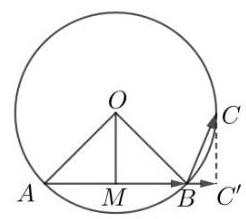
\includegraphics[max width=0.2\textwidth]{images/bo_d7fhnv491nqc73ercsbg_92_1163_1109_246_219_0.jpg}
\end{center}
\hspace*{3em} 

过点 \(O\) 作 \({OM} \bot  {AB}\) 交 \({AB}\) 于点 \(M,M\) 为 \({AB}\) 的中点,则 \({MB} = \frac{\sqrt{2}}{2}\) ,

\(M{C}^{\prime } = {OC} = 1\) ,则 \(\overrightarrow{BC}\) 在 \(\overrightarrow{AB}\) 方向上的数量投影为 \(\left| \overrightarrow{B{C}^{\prime }}\right|  = \left| {M{C}^{\prime }}\right|  - \left| {MB}\right|  = 1 - \frac{\sqrt{2}}{2}\) ,

所以 \({\left( \overrightarrow{AB} \cdot  \overrightarrow{BC}\right) }_{\max } = \left| \overrightarrow{AB}\right|  \cdot  \left| \overrightarrow{B{C}^{\prime }}\right|  = \sqrt{2} - 1\) ,故选 D.

13.(2025高三二模闵行 16)设 \(n\) 为正整数，空间中 \(n\) 个单位向量构成集合 \({A}_{n} = \left\{  {\overrightarrow{{a}_{1}},\overrightarrow{{a}_{2}},\cdots ,\overrightarrow{{a}_{n}}}\right\}\) ， 若存在实数 \(t\) ,满足对任意 \(\overrightarrow{{a}_{i}} \in  {A}_{n},\overrightarrow{{a}_{j}} \in  {A}_{n},\overrightarrow{{a}_{i}} \neq  \overrightarrow{{a}_{j}}\) ,都有 \(\overrightarrow{{a}_{i}} \cdot  \overrightarrow{{a}_{j}} = t\) ,则当 \(n\) 取得最大值时, \(t\) 的值为( ).

A. \(- \frac{1}{2}\) B. \(\frac{1}{2}\) C. \(- \frac{1}{3}\) D. \(\frac{1}{3}\)

【答案】C

【解析】令集合 \({A}_{n} = \left\{  {{\overrightarrow{a}}_{1},{\overrightarrow{a}}_{2},\cdots ,{\overrightarrow{a}}_{n}}\right\}\) 的各向量起点为 \(O\) ,对应终点依次为 \({A}_{1},{A}_{2},\cdots ,{A}_{n}\) , 由向量 \(\overrightarrow{{a}_{i}}\left( {i \in  {\mathrm{N}}^{ * },i \leq  n}\right)\) 为单位向量,则点 \({A}_{1},{A}_{2},\cdots ,{A}_{n}\) 在以 \(O\) 为球心,1 为半径的球面上,

由 \({\overrightarrow{a}}_{i} \in  {A}_{n},{\overrightarrow{a}}_{j} \in  {A}_{n},{\overrightarrow{a}}_{i} \neq  {\overrightarrow{a}}_{j}\) ,得点 \({A}_{1},{A}_{2},\cdots ,{A}_{n}\) 中任意三点不共线,

由 \(t = {\overrightarrow{a}}_{1} \cdot  {\overrightarrow{a}}_{2} = {\overrightarrow{a}}_{2} \cdot  {\overrightarrow{a}}_{3}\) ,得 \(\overrightarrow{O{A}_{2}} \cdot  \left( {\overrightarrow{O{A}_{1}} - \overrightarrow{O{A}_{3}}}\right)  = \overrightarrow{O{A}_{2}} \cdot  \overrightarrow{{A}_{3}{A}_{1}} = 0\) ,则 \(O{A}_{2} \bot  {A}_{1}{A}_{3}\) ,

由 \(t = {\overrightarrow{a}}_{4} \cdot  {\overrightarrow{a}}_{2} = {\overrightarrow{a}}_{2} \cdot  {\overrightarrow{a}}_{3}\) ,同理得 \(O{A}_{2} \bot  {A}_{4}{A}_{3}\) ,而点 \({A}_{1},{A}_{3},{A}_{4}\) 不共线,

于是点 \({A}_{1},{A}_{2},{A}_{3},{A}_{4}\) 不共面,点 \({A}_{1},{A}_{2},{A}_{3},{A}_{4}\) 为球 \(O\) 内接正四面体的 4 个顶点,

若 \(n \geq  5\) ,不妨取 \(n = 5\) ,同理得 \(O{A}_{5} \bot  {A}_{1}{A}_{3},O{A}_{5} \bot  {A}_{4}{A}_{3},O{A}_{5} \bot\) 平面 \({A}_{1}{A}_{3}{A}_{4}\) ,

又 \(O{A}_{5} \bot  {A}_{2}{A}_{3}\) ,由过一点有且只有一个平面垂直于已知直线,得点 \({A}_{2} \in\) 平面 \({A}_{1}{A}_{3}{A}_{4}\) ,

与点 \({A}_{1},{A}_{2},{A}_{3},{A}_{4}\) 不共面矛盾,因此 \({n}_{\max } = 4\) ,设正四面体 \({A}_{1}{A}_{2}{A}_{3}{A}_{4}\) 的棱长为 \(m\) ,

则正 \(\bigtriangleup {A}_{1}{A}_{2}{A}_{3}\) 的外接圆半径为 \(\frac{\sqrt{3}}{2}m \cdot  \frac{2}{3} = \frac{\sqrt{3}}{3}m\) ,正四面体的高为 \(\sqrt{{m}^{2} - {\left( \frac{3}{3}m\right) }^{2}} = \frac{\sqrt{6}}{3}m\) ,

球心到平面 \({A}_{1}{A}_{2}{A}_{3}\) 的距离为 \(\frac{\sqrt{6}}{3}m - 1\) ,因此 \({\left( \frac{\sqrt{6}}{3}m - 1\right) }^{2} + {\left( \frac{\sqrt{3}}{3}m\right) }^{2} = {1}^{2}\) ,解得 \(m = \frac{2\sqrt{6}}{3}\) ,

所以 \(t = \cos \angle {A}_{1}O{A}_{2} = \frac{{1}^{2} + {1}^{2} - {\left( \frac{2\sqrt{6}}{3}\right) }^{2}}{2 \times  1 \times  1} =  - \frac{1}{3}\) .

故选: C.

14.(2025 高三二模虹口 16)在空间中，点 \(O\) 、 \(A\) 均为定点，且 \(\left| \overrightarrow{OA}\right|  = 1\) . 设集合 \(S = \left\{  {P\left| {\;{\left| \overrightarrow{OP}\right| }^{2} - 2\overrightarrow{OA} \cdot  \overrightarrow{OP} \leq  1}\right. }\right\}\) ,则以下说法正确的是 ( ) .

 \circled{1}  若 \(\overrightarrow{OP}\) 在 \(\overrightarrow{OA}\) 上的数量投影为 \(- \frac{1}{5}\) ，则线段 \({OP}\) 在运动过程中所形成的几何体体积为 \(\frac{14}{375}\pi\)

 \circled{2}  对于任意的 \({P}_{i} \in  S\) 以及任意的正实数 \({a}_{i}\) ，设 \(\overrightarrow{OQ} = \mathop{\sum }\limits_{{i = 1}}^{4}{a}_{i}\overrightarrow{O{P}_{i}}\) ，若 \(\mathop{\sum }\limits_{{i = 1}}^{4}{a}_{i} = 1\) ，则 \(Q \in  S\) .

A.  \circled{1} 是真命题， \circled{2} 是真命题 B.  \circled{1} 是真命题， \circled{2} 是假命题

C.  \circled{1} 是假命题， \circled{2} 是真命题 D.  \circled{1} 是假命题， \circled{2} 是假命题

【答案】A

【解析】设 \(\overrightarrow{OA} = \left( {1,0,0}\right) ,P\left( {x,y,z}\right)\) ,

则 \({x}^{2} + {y}^{2} + {z}^{2} - {2x} \leq  1\) ,即 \({\left( x - 1\right) }^{2} + {y}^{2} + {z}^{2} \leq  2\) ,

\(P\) 在以 \(A = \left( {1,0,0}\right)\) 为圆心, \(r = \sqrt{2}\) 的球面及其内部,

对于 \circled{1} ,设点 \(B\) 是点 \(P\) 在 \({OA}\) 上的投影,则由 \(\left| {OP}\right| \cos \left\langle  {\overrightarrow{OP},\overrightarrow{OA}}\right\rangle   =  - \frac{1}{5}\) ,得 \(B\left( {-\frac{1}{5},0,0}\right)\) ,

\({\left| OP\right| }^{2} - 2\left| {OA}\right|  \cdot  \left| {OP}\right| \cos \left\langle  {\overrightarrow{OP},\overrightarrow{OA}}\right\rangle   \leq  1 \Rightarrow  {\left| OP\right| }^{2} \leq  \frac{3}{5},\)

\({\left| BP\right| }^{2} \leq  {\left| OP\right| }^{2} - {\left| OB\right| }^{2} = \frac{3}{5} - \frac{1}{25} = \frac{14}{25},\)

\(P\) 在圆 \(B\) 上及其内部,线段 \({OP}\) 在运动过程中所形成的几何体为圆锥,

\(V = \frac{1}{3}\pi  \cdot  B{P}^{2} \cdot  {OB} = \frac{14}{375}\pi\) , \circled{1}  对;

对于 \circled{2} ， \(\overrightarrow{OQ} = {a}_{1}\overrightarrow{O{P}_{1}} + {a}_{2}\overrightarrow{O{P}_{2}} + {a}_{3}\overrightarrow{O{P}_{3}} + {a}_{4}\overrightarrow{O{P}_{4}}\) ,

\({a}_{1} + {a}_{2} + {a}_{3} + {a}_{4} = 1,\overrightarrow{OQ} = {a}_{1}\overrightarrow{OP} + {a}_{2}\overrightarrow{O{P}_{2}} + {a}_{3}\overrightarrow{O{P}_{3}} + \left( {1 - {a}_{1} - {a}_{2} - {a}_{3}}\right) \overrightarrow{O{P}_{4}}\) ,

\(\overrightarrow{{P}_{4}Q} = {a}_{1}\overrightarrow{{P}_{4}{P}_{1}} + {a}_{2}\overrightarrow{{P}_{4}{P}_{2}} + {a}_{3}\overrightarrow{{P}_{4}{P}_{3}}\) ,由于 \({a}_{1} + {a}_{2} + {a}_{3} + {a}_{4} = 1,{a}_{1},{a}_{2},{a}_{3},{a}_{4} > 0\) ,

所以 \(0 < {a}_{1},{a}_{2},{a}_{3} < 1,{a}_{1} + {a}_{2} + {a}_{3} < 1\) ,所以点 \(Q\) 在四面体 \({P}_{1}{P}_{2}{P}_{3}{P}_{4}\) 上,

又由于 \(P\) 在球面及球内部, \(\therefore Q \in  S\) , \circled{2} 对;

故选 A.

\section*{二、向量的模}

1.(2025 高三二模嘉定 12)在平面直角坐标系中，一质点 \(P\) 从原点 \(O\) 出发，第一次从点 \(O\) 移动到点 \({P}_{1}\) ,第二次从点 \({P}_{1}\) 移动到点 \({P}_{2},\cdots\) ,第 \(k\) 次从点 \({P}_{k - 1}\) (规定 \({P}_{0} = O\) )移动到点 \({P}_{k}\) . 记向量 \(\overrightarrow{{v}_{k}} = \overrightarrow{{P}_{k - 1}{P}_{k}}\) ，其模长为 \(k\) ，方向与 \(x\) 轴正方向成 \({\left( {90}k\right) }^{ \circ  }\) 角. 设 \(\overrightarrow{{S}_{n}}\) 为经过 \(n\) 次移动的位移向量,即 \(\overrightarrow{{S}_{n}} = \overrightarrow{O{P}_{n}}\) ,则当 \(\left| \overrightarrow{{S}_{n}}\right|  = \sqrt{85}\) 时, \(n\) 的值为\_\_\_\_\_.

【答案】 13

【解析】由题意 \(\overrightarrow{{P}_{k - 1}{P}_{k}} = \left( {k\cos \left( {{90}^{ \circ  } \cdot  k}\right) ,k\sin \left( {{90}^{ \circ  } \cdot  k}\right) }\right)\) ,

\(\overrightarrow{{S}_{n}} = \overrightarrow{O{P}_{n}} = \overrightarrow{{P}_{0}{P}_{1}} + \overrightarrow{{P}_{1}{P}_{2}} + \cdots  + \overrightarrow{{P}_{n - 1}{P}_{n}} = \left( {\mathop{\sum }\limits_{{k = 1}}^{n}k\cos {90}^{ \circ  }k,\mathop{\sum }\limits_{{k = 1}}^{n}k\sin {90}^{ \circ  }k}\right)\) ,

当 \(n = {4m}\left( {m \in  {\mathbf{N}}^{ * }}\right)\) 时,

\(\mathop{\sum }\limits_{{k = 1}}^{n}k\cos {90}^{ \circ  }k =  - 2 + 4 - 6 + 8 + \cdots  - \left( {{4m} - 2}\right)  + {4m} = {2m},\)

\(\mathop{\sum }\limits_{{k = 1}}^{n}k\sin {90}^{ \circ  }k = 1 - 3 + 5 - 7 + \cdots  + \left( {{4m} - 3}\right)  - \left( {{4m} - 1}\right)  =  - {2m},\)

此时 \(\left| \overrightarrow{{S}_{n}}\right|  = \sqrt{{\left( 2m\right) }^{2} + {\left( -2m\right) }^{2}} = 2\sqrt{2}m = \sqrt{85}\) ,无整数解,舍; 当 \(n = {4m} - 1\left( {m \in  {\mathbf{N}}^{ * }}\right)\) 时,

\(\mathop{\sum }\limits_{{k = 1}}^{n}k\cos {90}^{ \circ  }k =  - 2 + 4 - 6 + 8 + \cdots  - \left( {{4m} - 2}\right)  =  - {2m}\)

\(\mathop{\sum }\limits_{{k = 1}}^{n}k\sin {90}^{ \circ  }k = 1 - 3 + 5 - 7 + \cdots  + \left( {{4m} - 3}\right)  - \left( {{4m} - 1}\right)  =  - {2m},\)

此时 \(\left| \overrightarrow{{S}_{n}}\right|  = \sqrt{{\left( -2m\right) }^{2} + {\left( -2m\right) }^{2}} = 2\sqrt{2}m = \sqrt{85}\) ,无整数解,舍;

当 \(n = {4m} - 2\left( {m \in  {\mathbf{N}}^{ * }}\right)\) 时,

\(\mathop{\sum }\limits_{{k = 1}}^{n}k\cos {90}^{ \circ  }k =  - 2 + 4 - 6 + 8 + \cdots  - \left( {{4m} - 2}\right)  =  - {2m}\)

\(\mathop{\sum }\limits_{{k = 1}}^{n}k\sin {90}^{ \circ  }k = 1 - 3 + 5 - 7 + \cdots  + \left( {{4m} - 3}\right)  = {2m} - 1,\)

此时 \(\left| \overline{{S}_{n}}\right|  = \sqrt{{\left( -2m\right) }^{2} + {\left( 2m - 1\right) }^{2}} = \sqrt{85}\) ,解得 \(m =  - 3\) 或 \(\frac{7}{2}\) ,舍;

当 \(n = {4m} - 3\left( {m \in  {\mathbf{N}}^{ * }}\right)\) 时,

\(\mathop{\sum }\limits_{{k = 1}}^{n}k\cos {90}^{ \circ  }k =  - 2 + 4 - 6 + 8 + \cdots  + \left( {{4m} - 4}\right)  = 2\left( {m - 1}\right) ,\)

\(\mathop{\sum }\limits_{{k = 1}}^{n}k\sin {90}^{ \circ  }k = 1 - 3 + 5 - 7 + \cdots  + \left( {{4m} - 3}\right)  = {2m} - 1,\)

此时 \(\left| \overrightarrow{{S}_{n}}\right|  = \sqrt{4{\left( m - 1\right) }^{2} + {\left( 2m - 1\right) }^{2}} = \sqrt{85}\) ,解得 \(m = 4\) 或 \(- \frac{5}{2}\) (舍),

所以 \(n = 4 \times  4 - 3 = {13}\) .

2.(2025 高三二模奉贤 12) \(\bigtriangleup  {ABC}\) 内一点 \(F\) (见图 12-1)，式子 \({FA} + {FC} + {FB}\) 可以写成 \(1 \times  {FA} + 1 \times  {FC} + 1 \times  {FB}\) ,这个式子中 \({FA},{FC},{FB}\) 的系数均为 1,以三个系数 1 作为边长可构造一个等边三角形,因此我们尝试把 \(\bigtriangleup {AFC}\) 绕点 \(C\) 顺时针旋转 \(\frac{\pi }{3}\) ,得到 \(\bigtriangleup {A}^{\prime }{F}^{\prime }C\) (见图 12-2), 所以 \({FA} + {FC} + {FB}\) 等于 \({F}^{\prime }{A}^{\prime } + {F}^{\prime }F + {FB}\) ，显然 \({F}^{\prime }{A}^{\prime } + {F}^{\prime }F + {FB} \geq  {A}^{\prime }B\) ，当 \({A}^{\prime },{F}^{\prime },F,B\) 四点共线时 (见图 12-3), \({FA} + {FC} + {FB}\) 最小.

\begin{center}
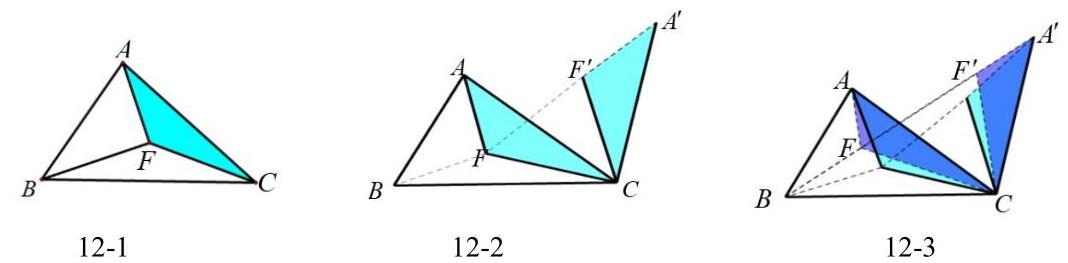
\includegraphics[max width=0.9\textwidth]{images/bo_d7fhnv491nqc73ercsbg_96_319_214_1068_263_0.jpg}
\end{center}
\hspace*{3em} 

第 12 题图

试用类似的方法解决下面这道题目:

已知 \(\overrightarrow{a}\) 是平面内的任意一个向量，向量 \(\overrightarrow{b},\overrightarrow{c}\) 满足 \(\overrightarrow{b} \cdot  \overrightarrow{c} = 0\) ，且 \(\left| \overrightarrow{b}\right|  = 4\) ， \(\left| \overrightarrow{c}\right|  = 4\) ， 则 \(\sqrt{2}\left| {\overrightarrow{a} - \overrightarrow{b}}\right|  + \left| {\overrightarrow{a} - \overrightarrow{c}}\right|  + \left| {\overrightarrow{a} + \overrightarrow{c}}\right|\) 的最小值为\_\_\_\_\_.

【答案】 \(8\sqrt{2}\)

【解析】设 \(\overrightarrow{OA} = \overrightarrow{a},\overrightarrow{OB} = \overrightarrow{b},\overrightarrow{OC} = \overrightarrow{c},\overrightarrow{O{C}^{\prime }} =  - \overrightarrow{c}\) ,

\(\sqrt{2}\left| {\overrightarrow{a} - \overrightarrow{b}}\right|  + \left| {\overrightarrow{a} - \overrightarrow{c}}\right|  + \left| {\overrightarrow{a} + \overrightarrow{c}}\right|  = \sqrt{2}{AB} + {AC} + \left| {\overrightarrow{OA} - \overrightarrow{O{C}^{\prime }}}\right|  = \sqrt{2}{AB} + {AC} + A{C}^{\prime }\) ,

将 \(\bigtriangleup {ABC}\) 绕点 \(B\) 顺时针旋转 \({90}^{ \circ  }\) 到 \({A}^{\prime }{B}^{\prime }{C}^{\prime \prime }\) ,

则 \(\angle {AB}{A}^{\prime } = {90}^{ \circ  }\) ,

\(A{A}^{\prime } = \sqrt{2}{AB},\sqrt{2}{AB} + {AC} + A{C}^{\prime } = A{A}^{\prime } + {A}^{\prime }{C}^{\prime \prime } + A{C}^{\prime }\) ,

设 \(\angle {ABC} = \angle {A}^{\prime }{B}^{\prime }C = \alpha\) ,

已知 \({OB} = {OC} = O{C}^{\prime } = 4,\angle {CB}{C}^{\prime } = {90}^{ \circ  },\therefore \angle {AB}{C}^{\prime } = {90}^{ \circ  } - \alpha\) ,

\(\angle {C}^{\prime }B{C}^{\prime \prime } = \angle {C}^{\prime }{BC} + \angle {CB}{C}^{\prime \prime } = {90}^{ \circ  } + {90}^{ \circ  } = {180}^{ \circ  }\) ,即 \(B,{C}^{\prime },{C}^{\prime \prime }\) 共线,

由题意得， \(A{A}^{\prime } + {A}^{\prime }{C}^{\prime \prime } + A{C}^{\prime } \leq  {C}^{\prime }{C}^{\prime \prime } = B{C}^{\prime } + B{C}^{\prime \prime } = B{C}^{\prime } + {BC} = 4\sqrt{2} + 4\sqrt{2} = 8\sqrt{2}\) , 当 \({C}^{\prime },A,{A}^{\prime },{C}^{\prime \prime }\) 四点共线时,取最小值.

\begin{center}
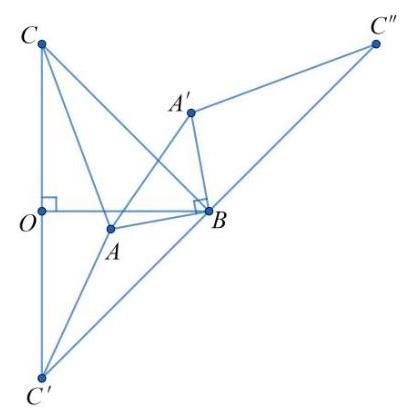
\includegraphics[max width=0.3\textwidth]{images/bo_d7fhnv491nqc73ercsbg_96_263_1577_407_416_0.jpg}
\end{center}
\hspace*{3em} 

\section*{三、复数的四则运算、复数的模}

1.(2025 高三二模宝山 1)已知 \(\mathrm{i}\) 是虚数单位，则 \(\left| {1 + \mathrm{i}}\right|  =\) \_\_\_\_\_.

【答案】 \(\sqrt{2}\)

【解析】 \(\left| {1 + \mathrm{i}}\right|  = \sqrt{{1}^{2} + {1}^{2}} = \sqrt{2}\) .

2.(2025 高三二模崇明 2)已知复数 \(\frac{z}{i} = 1 - {2i}\) ( \(i\) 为虚数单位)，则 \(z =\) \_\_\_\_\_.

【答案】 \(2 + i\)

【解析】 \(z = i\left( {1 - {2i}}\right)  = 2 + i\) .

3.(2025 高三二模金山 2)已知复数 \(z\) 满足 \(\left( {1 + i}\right) z = 1 - i\) (i 为虚数单位)，则 \(z =\) \_\_\_\_\_.

【答案】 \(- i\)

【解析】 \(z = \frac{1 - i}{1 + i} =  - i\) .

4. (2025 高三二模徐汇 2)复数 \(z = \frac{1}{1 - i}\) (其中 \(\mathrm{i}\) 为虚数单位)的虚部是\_\_\_\_\_.

【答案】 \(\frac{1}{2}\)

【解析】 \(z = \frac{1}{1 - i} = \frac{1}{2} + \frac{1}{2}i\) ,则复数 \(z\) 的虚部是 \(\frac{1}{2}\) .

5.(2025 高三二模奉贤 2)已知 \(\mathrm{i}\) 为虚数单位，复数 \(z\) 满足 \(z\mathrm{i} - \mathrm{i} = 1\) ，则 \(\left| z\right|  =\) \_\_\_\_\_.

【答案】 \(\sqrt{2}\)

【解析】 \(\left| z\right|  = \left| \frac{1 + i}{i}\right|  = \left| {1 - i}\right|  = \sqrt{2}\) .

6.(2025 高三二模长宁 2)复数 \({z}_{1} = 2 - {3\mathrm{i}},{z}_{2} = 1 - {2\mathrm{i}}\) ，则 \({z}_{1} \cdot  \overline{{z}_{2}} =\) \_\_\_\_\_.

【答案】 \(8 + \mathrm{i}\)

【解析】 \(\overline{{z}_{2}} = 1 + 2\mathrm{i}\) ,所以 \({z}_{1} \cdot  \overline{{z}_{2}} = \left( {2 - 3\mathrm{i}}\right) \left( {1 + 2\mathrm{i}}\right)  = 8 + \mathrm{i}\) .

7.(2025 高三二模普陀 2)已知复数 \(z = \frac{3 - {2\mathrm{i}}}{\mathrm{i}}\) ，其中 \(\mathrm{i}\) 为虚数单位，则 \(z + \bar{z} =\) \_\_\_\_\_.

【答案】 -4

【解析】 \(z = \frac{3 - 2\mathrm{i}}{\mathrm{i}} =  - 2 - 3\mathrm{i}\) ,则 \(\bar{z} =  - 2 + 3\mathrm{i}\) ,所以 \(z + \bar{z} =  - 4\) .

8.(2025 高三二模松江 3)若复数 \(z\) 满足 \(\frac{1 + \mathrm{i}}{z} = \mathrm{i}\) (其中 \(\mathrm{i}\) 是虚数单位)，则 \(\left| z\right|  =\) \_\_\_\_\_. 【答案】 \(\sqrt{2}\)

【解析】 \(\left| z\right|  = \left| \frac{1 + \mathrm{i}}{\mathrm{i}}\right|  = \frac{\left| 1 + \mathrm{i}\right| }{\left| \mathrm{i}\right| } = \frac{\sqrt{2}}{1} = \sqrt{2}\) .

9.(2025 高三二模闵行 3)已知 \(\mathrm{i}\) 是虚数单位，则 \(\left| \frac{1 + \mathrm{i}}{\mathrm{i}}\right|  =\) \_\_\_\_\_.

【答案】 \(\sqrt{2}\)

【解析】 \(\left| \frac{1 + i}{i}\right|  = \left| {1 - i}\right|  = \sqrt{{1}^{2} + {\left( -1\right) }^{2}} = \sqrt{2}\) .

10.(2025 高三二模黄浦 5) \(\mathrm{i}\) 为虚数单位，若复数 \(z\) 满足 \(z - \bar{z} = {2\mathrm{i}}\) 且 \(\bar{z} = \mathrm{i}z\) ，则 \(\operatorname{Re}z =\) \_\_\_\_\_.

【答案】 -1

【解析】设 \(z = a + b\mathrm{i}\) ,则 \(\bar{z} = a - b\mathrm{i}\) ,由题意 \(\left\{  {\begin{array}{l} a + b\mathrm{i} - \left( {a - b\mathrm{i}}\right)  = 2\mathrm{i} \\  a - b\mathrm{i} = \mathrm{i}\left( {a + b\mathrm{i}}\right)  \end{array} \Rightarrow  \left\{  \begin{array}{l} a =  - 1 \\  b = 1 \end{array}\right. }\right.\)

所以 \(\operatorname{Re}z =  - 1\) .

11.(2025 高三二模嘉定)已知复数 \({z}_{1},{z}_{2}\) 满足 \(\left| {z}_{1}\right|  = 1,\left| {z}_{2}\right|  = 2,\left| {{z}_{1} - {z}_{2}}\right|  = \sqrt{7}\) ，则 \(\left| {{z}_{1} + {z}_{2}}\right|\) 的值为\_\_\_\_\_.

【答案】 \(\sqrt{3}\)

【解析】由 \({\left| {z}_{1} + {z}_{2}\right| }^{2} + {\left| {z}_{1} - {z}_{2}\right| }^{2} = 2\left( {{\left| {z}_{1}\right| }^{2} + {\left| {z}_{2}\right| }^{2}}\right)\) ,得 \(\left| {{z}_{1} + {z}_{2}}\right|  = \sqrt{3}\) .

\section*{四、复数的几何意义、实系数的一元二次方程}

1.(2025 高三二模浦东 5)若关于 \(x\) 的方程 \({x}^{2} - x + m = 0\) 的一个虚根的模为 2，则实数 \(m\) 的值为\_\_\_\_\_.

【答案】 4

【解析】设方程一个虚根为 \(z\) ,则另一个虚根为 \(\bar{z}\) ,则 \(z \cdot  \bar{z} = {\left| z\right| }^{2} = m\) ,所以 \(m = 4\) .

2.(2025 高三二模杨浦 7)已知复数 \(z\) 满足 \(\left| {z - 1 + \mathrm{i}}\right|  = 1\) ，其中 \(\mathrm{i}\) 为虚数单位，则 \(\left| z\right|\) 的最小值为\_\_\_\_\_.

【答案】 \(\sqrt{2} - 1\)

【解析】由题意,复数 \(z\) 在复平面上是以 \(\left( {1, - 1}\right)\) 为圆心,1 为半径的圆上的点,所以 \(\left| z\right|\) 的最小值为 \(\sqrt{{\left( 1 - 0\right) }^{2} + {\left( -1 - 0\right) }^{2}} - 1 = \sqrt{2} - 1\) .

3. (2025 高三二模虹口 8) 已知 \(z\) 是实系数一元二次方程 \({x}^{2} + {px} + q = 0\) 的一个虚根,且 \(\left| {z - 1}\right|  = 2\) ,若 \(z\) 在复平面上所对应的点在抛物线 \({y}^{2} = {4x}\) 上,则 \(p =\) \_\_\_\_\_.

【答案】 -2

【解析】设 \(z = x + {yi}\) ,因为 \(\left| {z - 1}\right|  = 2\) ,则 \({\left( x - 1\right) }^{2} + {y}^{2} = 4\) ,

因为 \(z\) 在复平面上对应的点在抛物线 \({y}^{2} = {4x}\) 上,则联立方程 \(\left\{  \begin{array}{l} {\left( x - 1\right) }^{2} + {y}^{2} = 4 \\  {y}^{2} = {4x} \end{array}\right.\) ,

解得 \({x}_{1} = 1,{x}_{2} =  - 3\) (舍) \(\Rightarrow  \left\{  {\begin{array}{l} {x}_{1} = 1 \\  {y}_{1} =  \pm  2 \end{array} \Rightarrow  z = 1 + {2i}}\right.\) 或 \(z = 1 - {2i}\) ,

则 \(\bar{z} = 1 - {2i}\) 或 \(\bar{z} = 1 + {2i},\therefore z + \bar{z} =  - p = 2 \Rightarrow  p =  - 2\) .

4.(2025 高三二模青浦 9)已知复数 \(z\) 、 \(w\) 满足 \(\left| z\right|  = 2,z = \left( {1 + \mathrm{i}}\right) w\) (i 是虚数单位)，则 \(\left| {w + 2}\right|\) 的最大值是\_\_\_\_\_.

【答案】 \(2 + \sqrt{2}\)

【解析】方法一: \(\left| w\right|  = \left| \frac{z}{1 + \mathrm{i}}\right|  = \frac{\left| z\right| }{\left| 1 + \mathrm{i}\right| } = \sqrt{2}\) ,所以复数 \(w\) 在复平面上对应的点在以 \(\left( {0,0}\right)\) 为圆心, \(\sqrt{2}\) 为半径的圆上, \(\left| {w + 2}\right|\) 表示复数 \(w\) 在复平面上对应的点到 \(\left( {-2,0}\right)\) 的距离,易知最大值为 \(2 + \sqrt{2}\) .

方法二: 设 \(z = x + {yi}\) ,因为 \(\left| z\right|  = 2\) ,则 \({x}^{2} + {y}^{2} = 4\) ,

\(\therefore w = \frac{x + {yi}}{1 + i} = \left( {x + {yi}}\right) \left( {\frac{1}{2} - \frac{1}{2}i}\right)  = \left( {\frac{1}{2}x + \frac{1}{2}y}\right)  + \left( {-\frac{1}{2}x + \frac{1}{2}y}\right) i\) ,

\(\therefore \left| {w + 2}\right|  = \sqrt{{\left( \frac{1}{2}x + \frac{1}{2}y + 2\right) }^{2} + {\left( -\frac{1}{2}x + \frac{1}{2}y\right) }^{2}} = \sqrt{\frac{1}{2}{x}^{2} + \frac{1}{2}{y}^{2} + {2x} + {2y} + 4}\)

\(= \sqrt{{2x} + {2y} + 6}\) ,

设 \(x = 2\cos \alpha ,y = 2\sin \alpha\) ,

则 \(\left| {w + 2}\right|  = \sqrt{4\cos \alpha  + 4\sin \alpha  + 6} = \sqrt{4\sqrt{2}\sin \left( {\alpha  + \frac{\pi }{4}}\right)  + 6}\) ,

\(\therefore {\left| w + 2\right| }_{\max } = \sqrt{4\sqrt{2} + 6} = 2 + \sqrt{2}\) .

5.(2025 高三二模静安 14)若复数 \(z = \frac{a\mathrm{i}}{b + \mathrm{i}}\) ( \(a\text{ 、 }b \in  \mathbf{R}\) ， \(\mathrm{i}\) 是虚数单位)在复平面上对应的点位于第二象限, 则... ( )

A. \(a > 0\) 且 \(b > 0\) ； B. \(a > 0\) 且 \(b < 0\) ； C. \(a < 0\) 且 \(b > 0\) ； D. \(a < 0\) 且 \(b < 0\) .

【答案】D

【解析】 \(\because z = \frac{ai}{b + i} = \frac{{ai}\left( {b - i}\right) }{\left( {b + i}\right) \left( {b - i}\right) } = \frac{a + {abi}}{{b}^{2} + 1},\therefore \left\{  {\begin{array}{l} a < 0 \\  {ab} > 0 \end{array} \Rightarrow  \left\{  \begin{array}{l} a < 0 \\  b < 0 \end{array}\right. }\right.\) ,故选 D.

\section*{第六部分 解析几何}

\section*{一、直线的综合}

1. (2025 高三二模崇明 4)直线 \(x =  - 2\) 与直线 \(\sqrt{3}x - y + 1 = 0\) 的夹角为\_\_\_\_\_.

【答案】 \(\frac{\pi }{6}\)

【解析】两个直线的法向量为 \(\left( {1,0}\right)\) 和 \(\left( {\sqrt{3}, - 1}\right)\) ,则 \(\cos \alpha  = \frac{\left| \sqrt{3}\right| }{1 \times  \sqrt{3 + 1}} = \frac{\sqrt{3}}{2}\) , 则两个直线的夹角为 \(\frac{\pi }{6}\) .

2. (2025 高三二模奉贤 5)直线 \({3x} + {4y} - 5 = 0\) 上的动点 \(P\) 和直线 \({3x} + {4y} + {10} = 0\) 上的动点 \(Q\) ， 则点 \(P\) 与点 \(Q\) 之间距离的最小值是\_\_\_\_\_.

【答案】 3

【解析】由题意知点 \(P\) 与点 \(Q\) 之间距离的最小值即为两平行线之间的距离 \(\frac{\left| {10} + 5\right| }{\sqrt{{3}^{2} + {4}^{2}}} = 3\) .

3.(2025 高三二模奉贤 6)已知 \(\theta\) 是斜率为 -1 的直线的倾斜角，计算 \(\sin \left( {\theta  - \frac{\pi }{2}}\right)  =\) \_\_\_\_\_. 【答案】 \(\frac{\sqrt{2}}{2}\)

【解析】由题意知 \(\tan \theta  =  - 1,\therefore \theta  = \frac{3\pi }{4},\therefore \sin \left( {\theta  - \frac{\pi }{2}}\right)  = \sin \frac{\pi }{4} = \frac{\sqrt{2}}{2}\) .

\section*{二、圆的综合}

1. (2025 高三二模浦东 3)设圆 \(C\) 的方程为 \({x}^{2} + {y}^{2} + {4x} - {6y} + {10} = 0\) ，则圆 \(C\) 的半径为\_\_\_\_\_.

【答案】 \(\sqrt{3}\)

【解析】圆的方程配方可得 \({\left( x + 2\right) }^{2} + {\left( y - 3\right) }^{2} = 3\) ,所以半径为 \(\sqrt{3}\) .

2. (2025 高三二模虹口 5) 若直线 \(l\) 与直线 \(y = x\) 平行,且经过圆 \({x}^{2} - {2x} + {y}^{2} = 0\) 的圆心, 则 \(l\) 的方程为\_\_\_\_\_.

【答案】 \(y = x - 1\)

【解析】由题意知圆的标准方程为 \({\left( x - 1\right) }^{2} + {y}^{2} = 1\) ,圆心为 \(\left( {1,0}\right)\) 设直线方程为 \(y = x + t\) ,圆心 \(\left( {1,0}\right)\) 代入直线方程可得 \(t =  - 1\) ,则直线方程为 \(y = x - 1\) .

3. (2025 高三二模嘉定)的直线 \(l : y = x + 1\) 与圆 \(C : {x}^{2} + {y}^{2} - {4x} - {2y} = 0\) 所交得的弦长为\_\_\_\_\_.

【答案】 \(2\sqrt{3}\)

【解析】圆 \(C : {x}^{2} + {y}^{2} - {4x} - {2y} = 0\) 方程化为标准方程为 \({\left( x - 2\right) }^{2} + {\left( y - 1\right) }^{2} = 5\) , 圆的半径为 \(r = \sqrt{5}\) ,圆心到直线 \(l\) 的距离 \(d = \frac{\left| 2 - 1 + 1\right| }{\sqrt{{1}^{2} + {\left( -1\right) }^{2}}} = \sqrt{2}\) , 所以弦长 \(h = 2\sqrt{{r}^{2} - {d}^{2}} = 2\sqrt{3}\) .

4.(2025 高三二模黄浦 8)已知 \(a\) 为常数，圆 \({\left( x - a\right) }^{2} + {\left( y + a - 2\right) }^{2} = {r}^{2}\left( {r > 0}\right)\) 与圆 \({x}^{2} + {y}^{2} = 1\) 有公共点,当 \(r\) 取得最小值时, \(a\) 的值为\_\_\_\_\_.

【答案】 1

【解析】 \({\left( x - a\right) }^{2} + {\left( y + a - 2\right) }^{2} = {r}^{2}\) 的圆心为 \(C\left( {a,2 - a}\right)\) ,在直线 \(x + y - 2 = 0\) 上, 圆 \({x}^{2} + {y}^{2} = 1\) 的圆心 \(O\left( {0,0}\right)\) 到直线 \(x + y - 2 = 0\) 的距离 \(d = \frac{\left| -2\right| }{\sqrt{{1}^{2} + {1}^{2}}} = \sqrt{2} > 1\) , 所以当两圆有公共点时,圆 \({\left( x - a\right) }^{2} + {\left( y + a - 2\right) }^{2} = {r}^{2}\) 半径的最小值为 \(\sqrt{2} - 1\) ,此时 \({OC}\) 的连线与直线 \(x + y - 2 = 0\) 垂直,所以 \(\frac{2 - a}{a} = 1 \Rightarrow  a = 1\) .

5. (2025 高三二模松江 9) 已知点 \(P\) 为直线 \(l : x + y + 1 = 0\) 上的点,过点 \(P\) 作圆 \(N : {\left( x - 1\right) }^{2} + {\left( y - 1\right) }^{2} = 1\) 的切线 \({PA}\) ，切点为 \(A\) ，则 \(\cos \angle {PNA}\) 最大值为\_\_\_\_\_.

【答案】 \(\frac{\sqrt{2}}{3}\)

【解析】由题意,圆心 \(N\left( {1,1}\right) ,{PA} \bot  {NA}\) ,所以 \(\cos \angle {PNA} = \frac{NA}{NP}\) ,其中 \({NA} = r = 1\) , 若要余弦值取得最大,则 \({NP}\) 的长度取得最小,即 \({NP}\) 为圆心到直线的距离, \(d = \frac{\left| 1 + 1 + 1\right| }{\sqrt{{1}^{2} + {1}^{2}}} = \frac{3}{\sqrt{2}}\) ,所以 \({\left( \cos \angle {PNA}\right) }_{\max } = \frac{NA}{NP} = \frac{1}{\frac{3}{\sqrt{2}}} = \frac{\sqrt{2}}{3}\) .

6.(2025 高三二模金山 16)已知点 \(A\left( {{x}_{1},{y}_{1}}\right)\) 在圆 \({x}^{2} + {y}^{2} = 9\) 上，点 \(B\left( {{x}_{2},{y}_{2}}\right)\) 在圆 \({x}^{2} + {y}^{2} = {12}\) 上,且 \({x}_{1}{x}_{2} + {y}_{1}{y}_{2} = {x}_{1} + {x}_{2} - 1,O\) 为坐标原点.对于以下两个命题,判断正确的是( )

 \circled{1} 在坐标平面内存在点 \(P\) ,使得 \({AP}\bot {BP}\) 恒成立;

 \circled{2} 三角形 \({OAB}\) 面积的最小值为 \(\sqrt{22}\) .

A.  \circled{1} 是真命题， \circled{2} 是真命题 B.  \circled{1} 是假命题， \circled{2} 是真命题

C.  \circled{1} 是真命题， \circled{2} 是假命题 D.  \circled{1} 是假命题， \circled{2} 是假命题

【答案】A

【解析】因为

\({x}_{1}{x}_{2} + {y}_{1}{y}_{2} = {x}_{1} + {x}_{2} - 1 \Rightarrow  {x}_{1}{x}_{2} - {x}_{1} - {x}_{2} + 1 + {y}_{1}{y}_{2} = 0 \Rightarrow  \left( {{x}_{1} - 1}\right) \left( {{x}_{2} - 1}\right)  + {y}_{1}{y}_{2} = 0\)

\(P\left( {1,0}\right)\) ,则 \(\overrightarrow{PA} = \left( {{x}_{1} - 1,{y}_{1}}\right) ,\overrightarrow{PB} = \left( {{x}_{2} - 1,{y}_{2}}\right) ,\therefore \overrightarrow{PA} \cdot  \overrightarrow{PB} = 0\)

故在坐标平面内存在点 \(P\) ,使得 \({AP} \bot  {BP}\) 恒成立,故 \circled{1} 正确；

构造矩形 \({APBQ},O{A}^{2} + O{B}^{2} = O{Q}^{2} + O{P}^{2} \Rightarrow  9 + {12} = 1 + O{Q}^{2} \Rightarrow  O{Q}^{2} = {20}\) ,

则点 \(Q\) 在以 \(\left( {0,0}\right)\) 为圆心, \(2\sqrt{5}\) 为半径的圆上,

设 \(\angle {AOB} = \alpha\) ,又 \(\overrightarrow{OA} \cdot  \overrightarrow{OB} = \overrightarrow{OQ} \cdot  \overrightarrow{OP}\) ,

\(\therefore 3 \times  2\sqrt{3} \times  \cos \alpha  = 1 \times  2\sqrt{5} \times  \cos \angle {QOP} = t \in  \left\lbrack  {-2\sqrt{5},2\sqrt{5}}\right\rbrack\) ,

\(\therefore \cos \alpha  = \frac{t}{6\sqrt{3}},\therefore \sin \alpha  = \sqrt{1 - \frac{{t}^{2}}{108}}\) ,

\(\therefore {S}_{\bigtriangleup {OAB}} = \frac{1}{2} \times  3 \times  2\sqrt{3} \times  \sqrt{1 - \frac{{t}^{2}}{108}} = \frac{1}{2}\sqrt{{108} - {t}^{2}}\left( {t \in  \left\lbrack  {-2\sqrt{5},2\sqrt{5}}\right\rbrack  }\right)\) ,

当 \(t =  \pm  2\sqrt{5}\) 时, \(\bigtriangleup {AOB}\) 面积的最小值为 \(\frac{1}{2}\sqrt{{108} - {20}} = \frac{1}{2} \times  2\sqrt{22} = \sqrt{22}\) ,

故 \circled{2} 正确.

故选 A.

\section*{三、椭圆的综合}

1.(2025 高三二模静安 3)椭圆 \(\frac{{x}^{2}}{4} + \frac{{y}^{2}}{3} = 1\) 的离心率为\_\_\_\_\_.

【答案】 \(\frac{1}{2}\)

【解析】由题意知 \(a = 2,b = \sqrt{3},c = 1,\therefore e = \frac{c}{a} = \frac{1}{2}\) .

2.(2025 高三二模杨浦 11)如图，阿基米德椭圆规是由基座、带孔的横杆、两条互相垂直的空槽、连个可动滑块 \(A\) 、 \(B\) 组成的一种绘图工具,横杆的一端 \(C\) 上装有铅笔,假设两条互相垂直的空槽和带孔的横杆都足够长,将滑块 \(A\text{ 、 }B\) 固定在带孔的横杆上,令滑块 \(A\) 在中一条空槽上滑动,滑块 \(B\) 在另一条空槽上滑动,铅笔 \(C\) 随之运动就能画出椭圆. 当 \(A\text{ 、 }B\) 之间的距离为 14 厘米时，若需要画出一个离心率为 \(\frac{4}{5}\) 的椭圆，则 \(B\text{ 、 }C\) 之间的距离为\_\_\_\_\_ 厘米.

\begin{center}
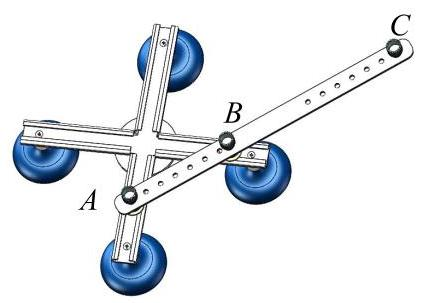
\includegraphics[max width=0.3\textwidth]{images/bo_d7fhnv491nqc73ercsbg_104_249_520_422_303_0.jpg}
\end{center}
\hspace*{3em} 

第 11 题图

【答案】 21

【解析】设 \({BC}\) 的长为 \(t\) ,当滑块 \(A\) 位于中心点时,可得 \(a = {14} + t\) ,当滑块 \(B\) 位于中心点时,可得 \(b = t\) ,又椭圆的离心率 \(e = \frac{c}{a} = \sqrt{1 - \frac{{b}^{2}}{{a}^{2}}} = \sqrt{1 - \frac{{t}^{2}}{{\left( {14} + t\right) }^{2}}} = \frac{4}{5}\) ,解得 \(t = {21}\) .

3. (2025 高三二模闵行 11)已知某星球的球心为 \(F\) ，半径为 \(R\) ，该星球的卫星的运行轨道是以 \(F\) 为一个焦点的椭圆,该椭圆的离心率为 \(\frac{3}{5}\) ,卫星运行过程中离该星球表面最近的距离为 \(R\) ,若当卫星处于某位置时,用卫星上的光学仪器观测该星球,把光学仪器的镜头与星球表面被观测点的连线称为视线, 任意两条视线所成的最大夹角称为张角, 则卫星运行过程中张角的最小值为\_\_\_\_\_. (精确到 \({0.1}^{ \circ  }\) )

【答案】 \({14.4}^{ \circ  }\)

【解析】设右顶点为 \(A\) ,左顶点为 \(B\) ,卫星离星球最近的位置为 \(A,a - c = {2R}\) , \(\sin \frac{\theta }{2} = {\left( \frac{R}{PF}\right) }_{\min } = \frac{R}{BF} = \frac{R}{a + c} = \frac{1}{2} \times  \frac{a - c}{a + c} = \frac{1}{2} \times  \frac{1 - e}{1 + e} = \frac{1}{2} \times  \frac{1 - \frac{3}{5}}{1 + \frac{3}{5}} = \frac{1}{8} \; \therefore \frac{\theta }{2} \approx  {7.18}^{ \circ  },\theta  \approx  {14.4}^{ \circ  }\) .

4.(2025 高三二模长宁 16)椭圆具有如下光学性质:如图， \({F}_{1}\left( {-c,0}\right)\) 、 \({F}_{2}\left( {c,0}\right)\) 分别是椭圆 \(\frac{{x}^{2}}{{a}^{2}} + \frac{{y}^{2}}{{b}^{2}} = 1\) 的左、右焦点,从点 \({F}_{1}\) 发出的光线在到达椭圆上的点 \(P\) 后,经过到达点的切线反射后经过点 \({F}_{2}\) ,有以下两个命题:

 \circled{1} 若 \(P\) 是椭圆上除长轴端点外的一点,设法线与 \(x\) 轴的交点为 \(M\left( {t,0}\right)\) ,则 \(t \in  \left( {-\frac{{c}^{2}}{a},\frac{{c}^{2}}{a}}\right)\) ;

\begin{center}
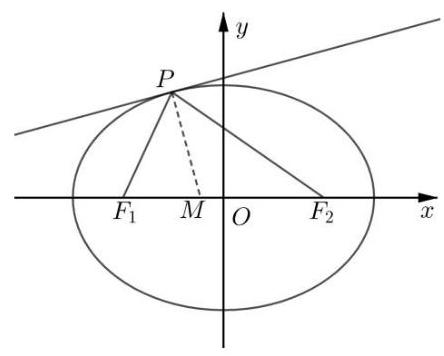
\includegraphics[max width=0.3\textwidth]{images/bo_d7fhnv491nqc73ercsbg_105_954_407_444_356_0.jpg}
\end{center}
\hspace*{3em} 

 \circled{2} 若从 \({F}_{1}\) 发出的光线，经椭圆两次反射后，第一次回到 \({F}_{1}\) 所经过的路程为 \({8c}\) ,则该椭圆的离心率为 \(\frac{1}{2}\) ;

则以下说法正确的是 ( )

A.  \circled{1} 是真命题， \circled{2} 是真命题

B.  \circled{1} 是真命题， \circled{2} 是假命题

C.  \circled{1} 是假命题， \circled{2} 是真命题

D.  \circled{1} 是假命题， \circled{2} 是假命题

【答案】A

【解析】 \circled{1}  设 \(P\left( {{x}_{0},{y}_{0}}\right)\) ,因为 \(\frac{{x}^{2}}{{a}^{2}} + \frac{{y}^{2}}{{b}^{2}} = 1\) ,所以 \(y =  \pm  b\sqrt{1 - \frac{{x}^{2}}{{a}^{2}}}\) ,

当 \(y = b\sqrt{1 - \frac{{x}^{2}}{{a}^{2}}}\) 时, \({y}^{\prime } = \frac{-\frac{b}{a}x}{\sqrt{{a}^{2} - {x}^{2}}}\) ,

所以在点 \(P\left( {{x}_{0},{y}_{0}}\right)\) 处的切线的斜率为 \(k = \frac{-\frac{b}{a}{x}_{0}}{\sqrt{{a}^{2} - {x}_{0}^{2}}} = \frac{-\frac{b}{a}{x}_{0}}{\sqrt{\frac{{a}^{2}{y}_{0}^{2}}{{b}^{2}}}} =  - \frac{{b}^{2}{x}_{0}}{{a}^{2}{y}_{0}}\) ,

同理可得当 \(y =  - b\sqrt{1 - \frac{{x}^{2}}{{a}^{2}}}\) 时,在点 \(P\left( {{x}_{0},{y}_{0}}\right)\) 处的切线的斜率为 \(k =  - \frac{{b}^{2}{x}_{0}}{{a}^{2}{y}_{0}}\) ,

所以椭圆 \(\frac{{x}^{2}}{{a}^{2}} + \frac{{y}^{2}}{{b}^{2}} = 1\) 在点 \(P\left( {{x}_{0},{y}_{0}}\right)\) 处的切线的斜率为 \(k =  - \frac{{b}^{2}{x}_{0}}{{a}^{2}{y}_{0}}\) ,

因为 \(M\left( {t,0}\right)\) ,所以 \({k}_{PM} = \frac{{y}_{0}}{{x}_{0} - t}\) ,

因为 \({k}_{PM} \cdot  k =  - 1\) ,所以 \(\frac{{y}_{0}}{{x}_{0} - t} \cdot  \left( {-\frac{{b}^{2}{x}_{0}}{{a}^{2}{y}_{0}}}\right)  =  - 1\) ,

所以 \(t = {x}_{0} - \frac{{b}^{2}{x}_{0}}{{a}^{2}} = \frac{{a}^{2}{x}_{0} - {b}^{2}{x}_{0}}{{a}^{2}} = \frac{{c}^{2}{x}_{0}}{{a}^{2}}\) ,

因为 \({x}_{0} \in  \left( {-a,a}\right)\) ,所以 \(t \in  \left( {-\frac{{c}^{2}}{a},\frac{{c}^{2}}{a}}\right)\) ,所以 \circled{1} 是真命题;

第 5 页(共 38 页)

 \circled{2} 因为 \({F}_{1}\) 发出的光线在到达椭圆上的点 \(P\) 后,经过到达点的切线反射后经过点 \({F}_{2}\) ，

所以两次反射后,第一次回到 \({F}_{1}\) 所经过的路程为 \({4a}\) ,

所以 \({4a} = {8c}\) ,所以 \(e = \frac{c}{a} = \frac{1}{2}\) ,所以 \circled{2} 是真命题.故选 A.

5.(2025 高三二模松江 20)已知椭圆 \(\Gamma  : \frac{{x}^{2}}{{a}^{2}} + \frac{{y}^{2}}{{b}^{2}} = 1\left( {a > b > 0}\right)\) 的左右焦点分别为 \({F}_{1}\text{ 、 }{F}_{2}\) ，上下顶点分别为 \({B}_{1}\text{ 、 }{B}_{2},\Delta {B}_{1}{F}_{1}{F}_{2}\) 是面积为 \(\sqrt{3}\) 的正三角形,过焦点的直线交椭圆 \(\Gamma\) 于 \(P\text{ 、 }Q\) 两点 \((P\text{ 、 }Q\) 分别在第一、四象限 \()\) .

(1)求椭圆 \(\Gamma\) 的离心率；

(2)已知点 \(M\left( {0,m}\right)\) ， \(m > 0\) ，求椭圆 \(\Gamma\) 上的动点 \(R\) 到点 \(M\) 的最大距离；

(3)求四边形 \({B}_{1}{B}_{2}{QP}\) 面积的取值范围.

【答案】(1) \(\frac{1}{2}\) ; (2) 当 \(0 < m < \frac{\sqrt{3}}{3}\) 时,最大距离为 \(2\sqrt{{m}^{2} + 1}\) ; 当 \(m \geq  \frac{\sqrt{3}}{3}\) 时,最大距离为 \(m + \sqrt{3};\left( 3\right) \left( {\frac{8\sqrt{3}}{5},\frac{3}{2} + \sqrt{3}}\right\rbrack\)

【解析】(1) 设椭圆 \(C\) 的焦距为 \(\left| {{F}_{1}{F}_{2}}\right|  = {2c}\left( {c > 0}\right)\) ,则 \(\left| {O{F}_{2}}\right|  = c\) ,

因为 \(\left| {O{B}_{1}}\right|  = b\) ,所以 \({Rt\Delta }{B}_{1}O{F}_{2}\) 中 \(\left| {{B}_{1}{F}_{2}}\right|  = a\) ,

又因为 \(\bigtriangleup {B}_{1}{F}_{1}{F}_{2}\) 为正三角形,所以 \(\left| {{B}_{1}{F}_{2}}\right|  = 2\left| {O{F}_{2}}\right|\) ,即 \(a = {2c}\) ,

所以椭圆的离心率 \(e = \frac{c}{a} = \frac{1}{2}\) . ...4 分

(2)由于正三角形 \({F}_{1}{F}_{2}{B}_{1}\) 的面积为 \(\sqrt{}3\) ，得到 \(\left\{  \begin{array}{l} \frac{\sqrt{3}}{2} = \frac{1}{2}\left| {{F}_{1}{F}_{2}}\right| b = {bc} \\  b = \frac{\sqrt{3}}{2} \times  {2c} = \sqrt{3}c \end{array}\right.\) ， 解得 \(c = 1,b = \sqrt{3}\) ,又 \({a}^{2} = {c}^{2} + {b}^{2}\) ,得到 \(a = 2\) ,故椭圆方程为 \(\frac{{x}^{2}}{4} + \frac{{y}^{2}}{3} = 1,\ldots 2\) 分设 \(R\left( {x,y}\right)\) ,且 \(\frac{{x}^{2}}{4} + \frac{{y}^{2}}{3} = 1\) ,即 \({x}^{2} = 4 - \frac{4{y}^{2}}{3}\) , \(\left| {RM}\right|  = \sqrt{{x}^{2} + {\left( y - m\right) }^{2}} = \sqrt{4 - \frac{4{y}^{2}}{3} + {y}^{2} - {2my} + {m}^{2}} = \sqrt{-\frac{1}{3}{y}^{2} - {2my} + {m}^{2} + 4},\) 其对称轴为 \(y =  - {3m} < 0\) ,而 \(- \sqrt{3} \leq  y \leq  \sqrt{3}\) ,当 \(- {3m} \leq   - \sqrt{3}\) ,即 \(m \geq  \frac{\sqrt{3}}{3}\) 时,

\(\left| {RM}\right|\) 在 \(y =  - \sqrt{3}\) 时取得最大值, \({\left| RM\right| }_{\max } = m + \sqrt{3}\) ; 2 分

当 \(0 >  - {3m} >  - \sqrt{3}\) ,即 \(0 < m < \frac{\sqrt{3}}{3}\) 时,

\(\left| {RM}\right|\) 在 \(y =  - {3m}\) 时取得最大值, \({\left| RM\right| }_{\max } = 2\sqrt{{m}^{2} + 1}\) . ...2 分

综上,当 \(0 < m < \frac{\sqrt{3}}{3}\) 时,最大距离为 \(2\sqrt{{m}^{2} + 1}\) ; 当 \(m \geq  \frac{\sqrt{3}}{3}\) 时,最大距离为 \(m + \sqrt{3}\) .

(3)设直线 \({PQ}\) 的方程为 \(x = {my} + 1,P\left( {{x}_{1},{y}_{1}}\right) ,Q\left( {{x}_{2},{y}_{2}}\right)\) ，

联立 \(\left\{  \begin{array}{l} x = {my} + 1 \\  \frac{{x}^{2}}{4} + \frac{{y}^{2}}{3} = 1 \end{array}\right.\) ,消去 \(x\) 整理得 \(\left( {3{m}^{2} + 4}\right) {y}^{2} + {6my} - 9 = 0\) ,

则 \(\Delta  > 0,{y}_{1} + {y}_{2} =  - \frac{6m}{3{m}^{2} + 4},{y}_{1}{y}_{2} =  - \frac{9}{3{m}^{2} + 4}\) . 2 分

因为点 \(P,Q\) 分别在第一、四象限,

所以 \(\left\{  \begin{array}{l} {x}_{1} + {x}_{2} > 0 \\  {x}_{1} \cdot  {x}_{2} > 0 \end{array}\right.\) ,即 \(\left\{  \begin{array}{l} m\left( {{y}_{1} + {y}_{2}}\right)  + 2 > 0 \\  {m}^{2}{y}_{1}{y}_{2} + m\left( {{y}_{1} + {y}_{2}}\right)  + 1 > 0 \end{array}\right.\) ,

故 \(\left\{  \begin{array}{l} \frac{-6{m}^{2}}{3{m}^{2} + 4} + 2 > 0 \\  \frac{-9{m}^{2}}{3{m}^{2} + 4} - \frac{6{m}^{2}}{3{m}^{2} + 4} + 1 > 0 \end{array}\right.\) ,解得 \(- \frac{\sqrt{3}}{3} < m < \frac{\sqrt{3}}{3}\) , ...2 分

得到四边形 \({B}_{1}{B}_{2}{QP}\) 的面积为 \(S = {S}_{\bigtriangleup O{B}_{1}P} + {S}_{\bigtriangleup O{B}_{2}Q} + {S}_{\bigtriangleup {OPQ}}\) ,

\(= \frac{1}{2}\left| {O{B}_{1}}\right|  \cdot  {x}_{1} + \frac{1}{2}\left| {O{B}_{2}}\right|  \cdot  {x}_{2} + \frac{1}{2}\left| {O{F}_{2}}\right|  \cdot  \left| {{y}_{1} - {y}_{2}}\right| ,\)

因为 \(\left| {{B}_{1}{B}_{2}}\right|  = 2\sqrt{3},{x}_{1} = m{y}_{1} + 1,{x}_{2} = m{y}_{2} + 1\) ,

所以 \(S = \frac{\sqrt{3}}{2}m\left( {{y}_{1} + {y}_{2}}\right)  + \sqrt{3} + \frac{1}{2}\sqrt{{\left( {y}_{1} + {y}_{2}\right) }^{2} - 4{y}_{1}{y}_{2}} = \frac{4\sqrt{3} + 6\sqrt{{m}^{2} + 1}}{3{m}^{2} + 4}\) , .2 分令 \(t = 4\sqrt{3} + 6\sqrt{{m}^{2} + 1},4\sqrt{3} + 6 \leq  t < 8\sqrt{3}\) ,则 \(S = \frac{t}{\frac{1}{12}{t}^{2} - \frac{2\sqrt{3}}{3}t + 5} = \frac{1}{\frac{t}{12} + \frac{5}{t} - \frac{2\sqrt{3}}{3}}\) ,

因为 \(4\sqrt{3} + 6 > 2\sqrt{15}\) ,所以 \(y = \frac{t}{12} + \frac{5}{t}\) 在 \(\lbrack 4\sqrt{3} + 6,8\sqrt{3})\) 上单调递增,

故 \(S \in  \left( {\frac{8\sqrt{3}}{5},\frac{3}{2} + \sqrt{3}}\right\rbrack\) ,即四边形 \({B}_{1}{B}_{2}{QP}\) 面积的取值范围为 \(\left( {\frac{8\sqrt{3}}{5},\frac{3}{2} + \sqrt{3}}\right\rbrack\) . ...2 分

6.(2025 高三二模青浦 20)如图，椭圆 \({C}_{1} : \frac{{x}^{2}}{8} + \frac{{y}^{2}}{{b}^{2}} = 1\left( {0 < b < 2\sqrt{2}}\right)\) 与双曲线 \({C}_{2} : \frac{{x}^{2}}{{b}^{2}} - {y}^{2} = 1\) 在第一象限的公共点为 \(A\left( {{x}_{A},{y}_{A}}\right) \left( {{x}_{A} > 0}\right)\) . 曲线 \(\Gamma\) 由两段曲线组成:当

\begin{center}
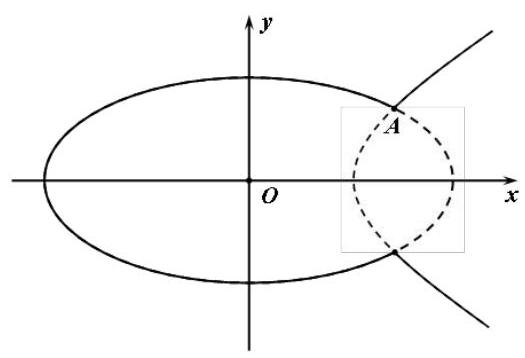
\includegraphics[max width=0.4\textwidth]{images/bo_d7fhnv491nqc73ercsbg_108_1016_692_525_358_0.jpg}
\end{center}
\hspace*{3em} 

\(x \leq  {x}_{A}\) 时,曲线 \(\Gamma\) 与椭圆 \({C}_{1}\) 重合,当 \(x > {x}_{A}\) 时,曲线 \(\Gamma\) 与双曲线 \({C}_{2}\) 重合.

(1)当 \({x}_{A} = 2\) 时，求 \(b\) 的值；

(2)已知 \(b = \sqrt{2}\) ，直线 \(l\) 过点 \(D\left( {2,0}\right)\) 与曲线 \(\Gamma\) 交于 \(E\) 、 \(F\) 两点,若 \(\overrightarrow{AD} \cdot  \overrightarrow{EF} = 2\) ,求直线 \(l\) 的方程;

(3)已知 \(A\left( {2,1}\right)\) ，斜率为 \(k\left( {k \geq  1}\right)\) 的直线 \(m\) 过点 \(P\left( {0,1}\right)\) 与曲线 \(\Gamma\) 交于 \(M\) 、 \(N\) 两点，若 \({S}_{\bigtriangleup {AMN}} = \lambda \tan \angle {MAN}\) ,求实数 \(\lambda\) 的最大值.

【答案】(1) \(b = \sqrt{2}\) ；(2) \(x = 2\) ；(3) \(\frac{14}{5}\)

【解析】(1) 根据题意,得, \(\left\{  \begin{array}{l} \frac{1}{2} + \frac{{y}^{2}}{{b}^{2}} = 1 \\  \frac{4}{{b}^{2}} - {y}^{2} = 1 \end{array}\right.\) ,解得 \(b = \sqrt{2}\) .

(2)由 \(\left\{  \begin{array}{l} \frac{{x}^{2}}{8} + \frac{{y}^{2}}{2} = 1 \\  \frac{{x}^{2}}{2} - {y}^{2} = 1 \end{array}\right.\) 得 \(A\left( {2,1}\right)\) ，

于是,曲线 \(\Gamma\) 的方程为: 当 \(x \leq  2\) 时, \(\frac{{x}^{2}}{8} + \frac{{y}^{2}}{2} = 1\) ,当 \(x > 2\) 时, \(\frac{{x}^{2}}{2} - {y}^{2} = 1\) .

易得, \(\overrightarrow{AD} = \left( {0, - 1}\right)\) ,

由于 \(\overrightarrow{AD} \cdot  \overrightarrow{EF} = 2\) ,故向量 \(\overrightarrow{EF}\) 在向量 \(\overrightarrow{AD}\) 方向上得数量投影大小为 -2 .

 \circled{1} 当直线 \(l\) 的斜率不存在时， \(l\) 与曲线 \(\Gamma\) 的两个交点为 \(\left( {2,1}\right) \text{ 、 }\left( {2, - 1}\right)\) ，取 \(E\text{ 、 }F\) 两点分别为 \(\left( {2, - 1}\right) \text{ 、 }\left( {2,1}\right)\) ,满足条件,此时直线 \(l\) 的方程为 \(x = 2\) .

 \circled{2} 当直线 \(l\) 的斜率存在时,设直线 \(l\) 方程为 \(x - 2 = {ty}\) ,根据对称性,只需考虑当 \(t > 0\) 的情况. 因为直线 \(l\) 与曲线 \(\Gamma\) 交于 \(E\text{ 、 }F\) 两点,故 \(t \in  \left( {0,\sqrt{2}}\right)\) .

由 \(\left\{  \begin{matrix} \frac{{x}^{2}}{2} - {y}^{2} = 1 \\  x - 2 = {ty} \end{matrix}\right.\) 得, \(\left( {{t}^{2} - 2}\right) {y}^{2} + {4ty} + 2 = 0\) ,解得, \(y = \frac{{2t} \pm  \sqrt{2{t}^{2} + 4}}{2 - {t}^{2}}\) ,

由于 \(4{t}^{2} - \left( {2{t}^{2} + 4}\right)  = 2\left( {{t}^{2} - 2}\right)  < 0\) ,

取 \({y}_{1} = \frac{{2t} + \sqrt{2{t}^{2} + 4}}{2 - {t}^{2}} > 0\) ,

又, \({y}_{1} - 1 = \frac{{2t} + \sqrt{2{t}^{2} + 4}}{2 - {t}^{2}} - 1 = \frac{{2t} + \sqrt{2{t}^{2} + 4} + {t}^{2} - 2}{2 - {t}^{2}}\) ,

因为, \(t \in  \left( {0,\sqrt{2}}\right)\) ,所以 \({y}_{1} > 1\) ,

由 \(\left\{  \begin{matrix} \frac{{x}^{2}}{8} + \frac{{y}^{2}}{2} = 1 \\  x - 2 = {ty} \end{matrix}\right.\) 得, \(\left( {{t}^{2} + 4}\right) {y}^{2} + {4ty} - 4 = 0\) ,解得, \(y = \frac{-{2t} \pm  2\sqrt{2{t}^{2} + 4}}{{t}^{2} + 4}\) ,

取 \({y}_{2} =  - \frac{{2t} + 2\sqrt{2{t}^{2} + 4}}{{t}^{2} + 4} < 0\) ,

因为, \(t \in  \left( {0,\sqrt{2}}\right)\) ,所以, \({2t} > {t}^{2}\) ,

又, \(2\sqrt{2{t}^{2} + 4} > 4\) ,所以, \(\frac{{2t} + 2\sqrt{2{t}^{2} + 4}}{{t}^{2} + 4} > 1\) ,故 \({y}_{2} <  - 1\) ,

所以向量 \(\overrightarrow{EF}\) 在向量 \(\overrightarrow{AD}\) 方向上的数量投影绝对值 \(\left| {{y}_{1} - {y}_{2}}\right|  > 1\) ,

即当直线 \(l\) 的斜率存在时,满足条件的直线 \(l\) 均不存在.

所以,满足条件的直线 \(l\) 的方程为 \(x = 2\) .

(3)根据题意，易得直线 \(m\) 只能与曲线 \(\Gamma\) 上 \(x \leq  2\) 时的曲线段相交.

令直线 \(m\) 方程为 \(y = {kx} + 1\left( {k \geq  1}\right)\) ,

由 \(\left\{  \begin{matrix} \frac{{x}^{2}}{8} + \frac{{y}^{2}}{2} = 1 \\  y = {kx} + 1 \end{matrix}\right.\) 得, \(\left( {4{k}^{2} + 1}\right) {x}^{2} + {8kx} - 4\) ,

设 \(M\left( {{x}_{1},{y}_{1}}\right) ,N\left( {{x}_{2},{y}_{2}}\right)\) 由韦达定理,得,

\[
\left\{  {\begin{matrix} \Delta  = {64}{k}^{2} + {16}\left( {4{k}^{2} + 1}\right)  > 0 \\  {x}_{1} + {x}_{2} =  - \frac{8k}{4{k}^{2} + 1} \\  {x}_{1}{x}_{2} =  - \frac{4}{4{k}^{2} + 1} \end{matrix},}\right.
\]

由 \({S}_{\bigtriangleup {AMN}} = \lambda \tan \angle {MAN}\) ,得, \(\frac{1}{2}\left| \overrightarrow{AM}\right| \left| \overrightarrow{AN}\right| \sin \angle {MAN} = \lambda \frac{\sin \angle {MAN}}{\cos \angle {MAN}}\) ,

变形,得, \(\overrightarrow{AM} \cdot  \overrightarrow{AN} = {2\lambda }\) ,

\(\overrightarrow{AM} = \left( {{x}_{1} - 2,{y}_{1} - 1}\right)  = \left( {{x}_{1} - 2,k{x}_{1}}\right) ,\overrightarrow{AN} = \left( {{x}_{2} - 2,{y}_{2} - 1}\right)  = \left( {{x}_{2} - 2,k{x}_{2}}\right)\) ,

于是, \(\left( {{x}_{1} - 2}\right) \left( {{x}_{2} - 2}\right)  + {k}^{2}{x}_{1}{x}_{2} = {2\lambda }\) ,

化简,得, \({x}_{1}{x}_{2} - 2\left( {{x}_{1} + {x}_{2}}\right)  + 4 + {k}^{2}{x}_{1}{x}_{2} = {2\lambda }\) ,

即 \(\frac{-4}{4{k}^{2} + 1} + 2\frac{8k}{4{k}^{2} + 1} + 4 - \frac{4{k}^{2}}{4{k}^{2} + 1} = {2\lambda }\) ,

变形,得 \(\lambda  = \frac{6{k}^{2} + {8k}}{4{k}^{2} + 1},k \geq  1\) ,

设 \(f\left( x\right)  = \frac{3{x}^{2} + {4x}}{4{x}^{2} + 1},x \geq  1\) ,

求导, \({f}^{\prime }\left( x\right)  = \frac{-{16}{x}^{2} + {6x} + 4}{{\left( 4{x}^{2} + 1\right) }^{2}}\) ,

由于, \(x \geq  1\) ,所以, \({f}^{\prime }\left( x\right)  < 0\) ,

所以 \(f\left( x\right)  = \frac{3{x}^{2} + {4x}}{4{x}^{2} + 1}\) 在 \(\lbrack 1, + \infty )\) 是严格减函数,

故,当 \(x = 1\) 时, \(f{\left( x\right) }_{\max } = \frac{7}{5}\) , 所以实数 \(\lambda\) 的最大值为 \(\frac{14}{5}\) .

7.(2025 高三二模普陀20)设 \(a > b > 0,m > 0\) ，点 \(A\) 、 \(F\) 分别是椭圆 \(\Gamma  : \frac{{x}^{2}}{{a}^{2}} + \frac{{y}^{2}}{{b}^{2}} = 1\) 的上顶点与右焦点,且 \(\left| {AF}\right|  = 2\) ,直线 \(l : x - {my} - 1 = 0\) 经过点 \(F\) 与 \(\Gamma\) 交于 \(P\text{ 、 }Q\) 两点, \(O\) 是坐标原点.

(1)求椭圆 \(\Gamma\) 的方程；

(2)若 \(m = \sqrt{3}\) ，点 \(M\) 是 \(x\) 轴上的一点，且 \(\bigtriangleup  {MPQ}\) 的面积为 \(\frac{6}{13}\) ，求点 \(M\) 的坐标；

(3)若点 \(G\) 在直线 \(x = 5\) 上,向量 \(\overrightarrow{PG}\) 在直线 \(l\) 上的投影为向量 \(\overrightarrow{PF}\) ,证明 \(\angle {PGQ} < \frac{\pi }{4}\) .

【答案】 \(\left( 1\right) \frac{{x}^{2}}{4} + \frac{{y}^{2}}{3} = 1\) ; (2) \(\left( {\frac{1}{2},0}\right)\) 或 \(\left( {\frac{3}{2},0}\right)\) ; (3) 证明见解析

【解析】(1) 由直线 \(l : x - {my} - 1 = 0\) 经过点 \(F\) ,得

点 \(F\left( {1,0}\right)\) ,又 \(\left| {AF}\right|  = 2\) ,则 \(a = 2\) , .2 分

即 \({b}^{2} = {a}^{2} - {c}^{2} = 3\) ,

则所求的椭圆 \(\Gamma\) 的方程为 \(\frac{{x}^{2}}{4} + \frac{{y}^{2}}{3} = 1\) .4 分

(2)设 \(P\left( {{x}_{1},{y}_{1}}\right)\) ， \(Q\left( {{x}_{1},{y}_{1}}\right)\) ， \(M\left( {{x}_{0},0}\right)\) ，

由 \(\left\{  \begin{array}{l} \frac{{x}^{2}}{4} + \frac{{y}^{2}}{3} = 1 \\  x = {my} + 1 \end{array}\right.\) 得， \(\left( {4 + 3{m}^{2}}\right) {y}^{2} + {6my} - 9 = 0\) ， .2 分

则 \({y}_{1} + {y}_{2} = \frac{-{6m}}{4 + 3{m}^{2}},{y}_{1}{y}_{2} = \frac{-9}{4 + 3{m}^{2}}\) ,

又 \(m = \sqrt{3}\) ,则 \(\left| {{y}_{1} - {y}_{2}}\right|  = \sqrt{{\left( {y}_{1} + {y}_{2}\right) }^{2} - 4{y}_{1}{y}_{2}} = \frac{24}{13}\) ,

又 \(\bigtriangleup  {MPQ}\) 的面积为 \(\frac{6}{13}\) ，

则 \({S}_{\bigtriangleup {MPQ}} = \frac{1}{2}\left| {MF}\right|  \cdot  \left| {{y}_{1} - {y}_{2}}\right|  = \frac{1}{2} \times  \frac{24}{13}\left| {{x}_{0} - 1}\right|  = \frac{6}{13}\) ， .4 分

即 \(\left| {{x}_{0} - 1}\right|  = \frac{1}{2}\) ,即 \({x}_{0} = \frac{1}{2}\) 或 \(\frac{3}{2}\) ,

则所求的点 \(M\) 的坐标为 \(\left( {\frac{1}{2},0}\right)\) 或 \(\left( {\frac{3}{2},0}\right)\) . .6 分

(3)由点 \(G\) 在直线 \(x = 5\) 上，向量 \(\overrightarrow{PG}\) 在直线 \(l\) 上的投影为向量 \(\overrightarrow{PF}\) ，得

\({GF} \bot  {PQ}\) ,且点 \(G\) 的坐标为 \(\left( {5, - {4m}}\right)\) , .2 分

又 \({x}_{1} = m{y}_{1} + 1,{x}_{2} = m{y}_{2} + 1\) ,

则 \(\left| {QF}\right|  = \sqrt{1 + {m}^{2}}\left| {y}_{2}\right| ,\left| {PF}\right|  = \sqrt{1 + {m}^{2}}\left| {y}_{1}\right| ,\left| {GF}\right|  = 4\sqrt{1 + {m}^{2}}\) ,

因为 \(m > 0,{GF} \bot  {PQ}\) ,所以在 \({\Delta GFP}\) 和 \({\Delta GFQ}\) 中分别有

\(\tan \angle {PGF} = \frac{\left| PF\right| }{\left| GF\right| } = \frac{\left| {y}_{1}\right| }{4},\tan \angle {QGF} = \frac{\left| QF\right| }{\left| GF\right| } = \frac{\left| {y}_{2}\right| }{4},\)

则 \(\tan \angle {PGQ} = \tan \left( {\angle {PGF} + \angle {QGF}}\right)  = \frac{\frac{\left| {y}_{1}\right| }{4} + \frac{\left| {y}_{2}\right| }{4}}{1 - \frac{\left| {y}_{1}\right| }{4} \cdot  \frac{\left| {y}_{2}\right| }{4}}\) ,

化简整理得, \(\tan \angle {PGQ} = \frac{4\left( {\left| {y}_{1}\right|  + \left| {y}_{2}\right| }\right) }{{16} - \left| {y}_{1}\right| \left| {y}_{2}\right| } = \frac{4\left| {{y}_{1} - {y}_{2}}\right| }{{16} - \left| {{y}_{1}{y}_{2}}\right| }\) , .4 分

由 (2) 中得, \({y}_{1} + {y}_{2} = \frac{-{6m}}{4 + 3{m}^{2}},{y}_{1}{y}_{2} = \frac{-9}{4 + 3{m}^{2}}\) ,

则 \(\tan \angle {PGQ} = \frac{{48}\sqrt{1 + {m}^{2}}}{{48}{m}^{2} + {55}}\) , .6 分

令 \(h = \sqrt{1 + {m}^{2}}\) ,则 \(\tan \angle {PGQ} = \frac{48}{{48h} + \frac{7}{h}}\) ,

设函数 \(g\left( h\right)  = {48h} + \frac{7}{h}\) ,则 \({g}^{\prime }\left( h\right)  = {48} - \frac{7}{{h}^{2}}\) ,因为 \(m > 0\) ,所以 \(h > 1\) ,

则 \({g}^{\prime }\left( h\right)  > 0\) ,即函数 \(g\left( h\right)  = {48h} + \frac{7}{h}\) 在区间 \(\left( {1, + \infty }\right)\) 上是严格增函数,

则 \(g\left( h\right)  > g\left( 1\right)  = {55}\) ,即 \(0 < \tan \angle {PGQ} < \frac{48}{55} < 1\) ,

则 \(\angle {PGQ} < \frac{\pi }{4}\) . 8 分

8.(2025 高三二模黄浦 20)椭圆 \(\Gamma  : \frac{{x}^{2}}{{a}^{2}} + \frac{{y}^{2}}{{b}^{2}} = 1\left( {a > b > 0}\right)\) 的左、右焦点分别为 \({F}_{1}\left( {-c,0}\right) ,{F}_{2}\left( {c,0}\right) \left( {c > 0}\right)\) ,过点 \({F}_{1}\) 的直线 \(l\) 与 \(\Gamma\) 交于点 \(P\) .

(1)若 \(c = 2\) ，点 \(P\) 的坐标为 \(\left( {2,\sqrt{2}}\right)\) ，求点 \({F}_{2}\) 到直线 \(l\) 的距离；

(2)当 \(b \leq  c\) 时，求满足 \(P{F}_{1} \bot  P{F}_{2}\) 的点 \(P\) 的个数；

(3)设直线 \(l\) 与 \(\Gamma\) 的另一个交点为 \(Q,\overrightarrow{{F}_{1}Q} = \lambda \overrightarrow{QP}\left( {\lambda  \in  \mathbf{R}}\right)\) ，点 \(P\) 的横坐标为 \(\frac{c}{2}\) ，若 \(\Gamma\) 的离心率 \(e > \frac{1}{2}\) ,求 \(\lambda\) 的取值范围.

【答案】(1) \(\frac{4}{3}\) ; (2) 当 \(b = c\) 时,点 \(P\) 的个数为 2; 当 \(b < c\) 时,点 \(P\) 的个数为 4; (3) \(- \frac{1}{3} < \lambda  < 0\) .

【解析】(1) 依题意, \({F}_{1}\left( {-2,0}\right) ,{F}_{2}\left( {2,0}\right)\) ,而 \(P\left( {2,\sqrt{2}}\right)\) ,则直线 \(l\) 的方程为 \(y = \frac{\sqrt{2}}{4}\left( {x + 2}\right)\) , 即 \(x - 2\sqrt{2}y + 2 = 0\) ,所以点 \({F}_{2}\) 到直线 \(l\) 的距离 \(d = \frac{\left| 2 - 2\sqrt{2} \times  0 + 2\right| }{\sqrt{{1}^{2} + {\left( -2\sqrt{2}\right) }^{2}}} = \frac{4}{3}\) .

(2)由 \(P{F}_{1} \bot  P{F}_{2}\) ，得点 \(P\) 在以线段 \({F}_{1}{F}_{2}\) 为直径的圆 \({x}^{2} + {y}^{2} = {c}^{2}\) 上， \({c}^{2} = {a}^{2} - {b}^{2}\) ， 由 \(\left\{  \begin{array}{l} {x}^{2} + {y}^{2} = {c}^{2} \\  {b}^{2}{x}^{2} + {a}^{2}{y}^{2} = {a}^{2}{b}^{2} \end{array}\right.\) 消去 \(y\) 得 \(\left( {{a}^{2} - {b}^{2}}\right) {x}^{2} = {a}^{2}\left( {{c}^{2} - {b}^{2}}\right)\) ,即 \({c}^{2}{x}^{2} = {a}^{2}\left( {{c}^{2} - {b}^{2}}\right)\) , 当 \(b = c\) 时, \(x = 0,y =  \pm  b\) ,因此点 \(P\left( {0, \pm  b}\right)\) ,共 2 个; 当 \(b < c\) 时, \({c}^{2}{x}^{2} = {a}^{2}\left( {{c}^{2} - {b}^{2}}\right)\) ,解得 \({x}^{2} = \frac{{a}^{2}\left( {{c}^{2} - {b}^{2}}\right) }{{c}^{2}},{y}^{2} = \frac{{b}^{4}}{{c}^{2}}\) , 因此点 \(P\left( {\pm \frac{a\sqrt{{c}^{2} - {b}^{2}}}{c}, \pm  \frac{{b}^{2}}{c}}\right)\) ,共 4 个, 所以当 \(b = c\) 时,点 \(P\) 的个数为 2; 当 \(b < c\) 时,点 \(P\) 的个数为 4 .

(3)设 \(P\left( {\frac{c}{2},{y}_{P}}\right) ,Q\left( {{x}_{Q},{y}_{Q}}\right)\) ，由 \(\overrightarrow{{F}_{1}Q} = \lambda \overrightarrow{QP}\) ，且 \({F}_{1}\) 在线段 \({PQ}\) 上，得 \(- 1 < \lambda  < 0\) ，

则 \(\left( {{x}_{Q} + c,{y}_{Q}}\right)  = \lambda \left( {\frac{c}{2} - {x}_{Q},{y}_{P} - {y}_{Q}}\right)\) ,解得 \(\left\{  \begin{array}{l} {x}_{Q} = \frac{c}{2} \cdot  \frac{\lambda  - 2}{\lambda  + 1} \\  {y}_{Q} = \frac{\lambda }{\lambda  + 1}{y}_{P} \end{array}\right.\) ,而 \(e = \frac{c}{a}\) ,

由点 \(P,Q\) 在 \(\Gamma\) 上,得 \(\left\{  \begin{array}{l} \frac{{c}^{2}}{4{a}^{2}} + \frac{{y}_{P}^{2}}{{b}^{2}} = 1 \\  \frac{{c}^{2}{\left( \lambda  - 2\right) }^{2}}{4{a}^{2}{\left( \lambda  + 1\right) }^{2}} + \frac{{\lambda }^{2}}{{\left( \lambda  + 1\right) }^{2}} \cdot  \frac{{y}_{P}^{2}}{{b}^{2}} = 1 \end{array}\right.\) ,

\begin{center}
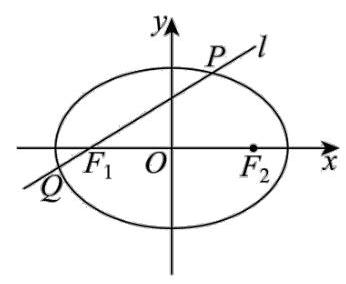
\includegraphics[max width=0.2\textwidth]{images/bo_d7fhnv491nqc73ercsbg_113_1080_1831_346_284_0.jpg}
\end{center}
\hspace*{3em} 

即 \(\left\{  \begin{array}{l} \frac{{e}^{2}}{4} + \frac{{y}_{P}^{2}}{{b}^{2}} = 1 \\  \frac{{e}^{2}{\left( \lambda  - 2\right) }^{2}}{4{\lambda }^{2}} + \frac{{y}_{P}^{2}}{{b}^{2}} = \frac{{\left( \lambda  + 1\right) }^{2}}{{\lambda }^{2}} \end{array}\right.\) ,

整理得 \({e}^{2}\left( {-\lambda  + 1}\right)  = {2\lambda } + 1\) ,即 \({e}^{2} = \frac{{2\lambda } + 1}{-\lambda  + 1}\) ,由 \(e > \frac{1}{2}\) ,得 \(\frac{1}{4} < \frac{{2\lambda } + 1}{-\lambda  + 1} < 1\) ,解得 \(- \frac{1}{3} < \lambda  < 0\) , 所以 \(\lambda\) 的取值范围是 \(- \frac{1}{3} < \lambda  < 0\) .

9.(2025 高三二模金山 20)已知椭圆 \(\Gamma  : \frac{{x}^{2}}{4} + \frac{{y}^{2}}{3} = 1\) ，左右焦点分别为 \({F}_{1}\) 、 \({F}_{2}\) ，上下顶点分别为 \(A\) 、 \(B\) ，左右顶点分别为 \(C\) 、 \(D\) ， \(P\) 、 \(Q\) 是 \(\Gamma\) 上异于椭圆顶点的两点.

(1)求 \(\bigtriangleup  A{F}_{1}{F}_{2}\) 的周长;

(2)若点 \(Q\) 在第一象限且满足 \(\bigtriangleup  {ABQ}\) 的面积比 \(\bigtriangleup  {{F}_{1}{F}_{2}Q}\) 的面积大，求点 \(Q\) 的横坐标的取值范围;

(3)记点 \(A\) 在直线 \({PQ}\) 上的投影为 \(H\) ，且直线 \({CP}\) 的斜率是直线 \({DQ}\) 的斜率的 3 倍，试判断: 过点 \(A\text{ 、 }H\text{ 、 }O\left( {O\text{ 为坐标原点 }}\right)\) 三点的圆是否为定圆? 若是,求出该圆的方程; 若不是,请说明理由.

【答案】(1) \(6;\left( 2\right) \left( {\frac{2\sqrt{5}}{5},2}\right) ;\left( 3\right)\) 过点 \(A\text{ 、 }H\text{ 、 }O\) 三点的圆是定圆 \({\left( x + \frac{1}{2}\right) }^{2} + {\left( y - \frac{\sqrt{3}}{2}\right) }^{2} = 1\)

【解析】(1)解: 由题意: \({a}^{2} = 4,{b}^{2} = 3,{c}^{2} = {a}^{2} - {b}^{2} = 4 - 3 = 1\) ,

得: \(a = 2,c = 1\) , .2 分

因此 \(\bigtriangleup A{F}_{1}{F}_{2}\) 的周长为 \({2a} + {2c} = 6\) . 4 分

(2)设 \(Q\left( {x,y}\right) \left( {x > 0,y > 0}\right)\) ，

\(A\left( {0,\sqrt{3}}\right) ,B\left( {0, - \sqrt{3}}\right) ,{F}_{1}\left( {-1,0}\right) ,{F}_{2}\left( {1,0}\right) ,\)

\({S}_{\bigtriangleup }{ABQ} = \frac{1}{2}\left| {AB}\right|  \cdot  \left| x\right|  = \sqrt{3}x;{S}_{\bigtriangleup }{F}_{1}{F}_{2}Q = \frac{1}{2}\left| {{F}_{1}{F}_{2}}\right|  \cdot  \left| y\right|  = y,\) 6 分

\(\left\{  {\begin{array}{l} \sqrt{3}x > y > 0 \\  \frac{{x}^{2}}{4} + \frac{{y}^{2}}{3} = 1 \end{array},\text{ 解得 }x \in  \left( {\frac{2\sqrt{5}}{5},2}\right) ,}\right.\)

即点 \(Q\) 的横坐标取值范围为 \(\left( {\frac{2\sqrt{5}}{5},2}\right)\) . 10 分

(3)过点 \(A\) 、 \(H\) 、 \(O\left( {O\text{ 为坐标原点 }}\right)\) 三点的圆是定圆. 11 分

法一:

设 \({l}_{PQ} : \left\{  \begin{array}{l} x = {my} + n \\  3{x}^{2} + 4{y}^{2} = {12} \end{array}\right.\) ,

得 \(\left( {3{m}^{2} + 4}\right) {y}^{2} + {6mny} + 3{n}^{2} - {12} = 0\) ,

\(\Delta  = {36}{m}^{2}{n}^{2} - 4\left( {3{m}^{2} + 4}\right) \left( {3{n}^{2} - {12}}\right)\)

\(= {48}\left( {3{m}^{2} - {n}^{2} + 4}\right)  > 0\) ,

设 \(P\left( {{x}_{1},{y}_{1}}\right) ,Q\left( {{x}_{2},{y}_{2}}\right)\) ,

\({y}_{1} + {y}_{2} = \frac{-{6mn}}{3{m}^{2} + 4},\;{y}_{1}{y}_{2} = \frac{3{n}^{2} - {12}}{3{m}^{2} + 4},\) 13 分

由题意 \({k}_{CP} = 3{k}_{DQ}\) ,即 \(\frac{{y}_{1}}{{x}_{1} + 2} = \frac{3{y}_{2}}{{x}_{2} - 2}\) ,

\({y}_{1}\left( {m{y}_{2} + n - 2}\right)  = 3{y}_{2}\left( {m{y}_{1} + n + 2}\right) .\) 14 分

即 \({2m}{y}_{1}{y}_{2} + 3\left( {n + 2}\right) {y}_{2} - \left( {n - 2}\right) {y}_{1} = 0\) .

\(\frac{{2m}\left( {3{n}^{2} - {12}}\right) }{3{m}^{2} + 4} + 4\left( {n + 1}\right) {y}_{2} - \left( {n - 2}\right) \left( {{y}_{1} + {y}_{2}}\right)  = 0,\)

\(\frac{{6m}\left( {{n}^{2} - 4}\right) }{3{m}^{2} + 4} - \left( {n - 2}\right)  \cdot  \frac{-{6mn}}{3{m}^{2} + 4} + 4\left( {n + 1}\right) {y}_{2} = 0,\)

\(\frac{{12m}\left( {n - 2}\right) \left( {n + 1}\right) }{3{m}^{2} + 4} + 4\left( {n + 1}\right) {y}_{2} = 0,\)

\(4\left( {n + 1}\right) \left\lbrack  {\frac{{3m}\left( {n - 2}\right) }{3{m}^{2} + 4} + {y}_{2}}\right\rbrack   = 0,\)

\(n =  - 1,\)

即 \({l}_{PQ}\) 过定点 \(\left( {-1,0}\right)\) . 16 分

设 \(H\left( {x,y}\right)\) ,

\(\left( {x + 1}\right) x + y\left( {y - \sqrt{3}}\right)  = 0\) 过原点,

即过点 \(A\text{ 、 }H\text{ 、 }O\left( O\right.\) 为坐标原点 \()\) 三点的圆是定圆 \({\left( x + \frac{1}{2}\right) }^{2} + {\left( y - \frac{\sqrt{3}}{2}\right) }^{2} = 1\) .

18 分

法二: 设 \({l}_{CP} : y = {3k}\left( {x + 2}\right) ,{l}_{DQ} : y = k\left( {x - 2}\right) \left( {k \neq  0}\right)\) , 12 分

联立 \(\left\{  \begin{array}{l} \frac{{x}^{2}}{4} + \frac{{y}^{2}}{3} = 1, \\  y = k\left( {x - 2}\right)  \end{array}\right.\)

消元得: \(\left( {4{k}^{2} + 3}\right) {x}^{2} - {16}{k}^{2}x + {16}{k}^{2} - {12} = 0\) ,

则 \(2{x}_{Q} = \frac{{16}{k}^{2} - {12}}{4{k}^{2} + 3}\) 得 \(Q\left( {\frac{8{k}^{2} - 6}{4{k}^{2} + 3},\frac{-{12k}}{4{k}^{2} + 3}}\right)\) , 13 分

同理联立 \(\left\{  \begin{array}{l} \frac{{x}^{2}}{4} + \frac{{y}^{2}}{3} = 1 \\  y = {3k}\left( {x + 2}\right)  \end{array}\right.\) ,

\(\left( {{12}{k}^{2} + 1}\right) {x}^{2} + {48}{k}^{2}x + {48}{k}^{2} - 4 = 0,\)

\(- 2 \cdot  {x}_{p} = \frac{{48}{k}^{2} - 4}{{12}{k}^{2} + 1}\) 得 \(P\left( {\frac{-{24}{k}^{2} + 2}{{12}{k}^{2} + 1},\frac{12k}{{12}{k}^{2} + 1}}\right)\) . 14 分

 \circled{1}  当 \({x}_{p} \neq  {x}_{Q}\) 即 \({k}^{2} \neq  \frac{1}{4}\) 时，

\({k}_{PQ} = \frac{\frac{12k}{{12}{k}^{2} + 1} - \frac{-{12k}}{4{k}^{2} + 3}}{\frac{-{24}{k}^{2} + 2}{{12}{k}^{2} + 1} - \frac{8{k}^{2} - 6}{4{k}^{2} + 3}} = \frac{4k}{1 - 4{k}^{2}},\)

\({l}_{PQ} : y + \frac{12k}{4{k}^{2} + 3} = \frac{4k}{1 - 4{k}^{2}}\left( {x - \frac{8{k}^{2} - 6}{4{k}^{2} + 3}}\right) ,\)

即 \(y = \frac{4k}{1 - 4{k}^{2}}\left( {x + 1}\right)\) ,过 \(\left( {-1,0}\right)\) . 15 分

 \circled{2}  当 \({x}_{P} = {x}_{Q}\) 即 \({k}^{2} = \frac{1}{4}\) 时，

此时 \({x}_{P} = {x}_{Q} =  - 1\) ,也过 \(\left( {-1,0}\right)\) ,

故 \({l}_{PQ}\) 过定点 \(\left( {-1,0}\right)\) , 16 分

设 \(H\left( {x,y}\right)\) ,

\(\left( {x + 1}\right) x + y\left( {y - \sqrt{3}}\right)  = 0\) 过原点,

即过点 \(A\text{ 、 }H\text{ 、 }O\left( O\right.\) 为坐标原点 \()\) 三点的圆是定圆 \({\left( x + \frac{1}{2}\right) }^{2} + {\left( y - \frac{\sqrt{3}}{2}\right) }^{2} = 1\) .

10.(2025 高三二模嘉定 20)已知椭圆 \(C : \frac{{x}^{2}}{9} + {y}^{2} = 1\) . \(F\) 为椭圆的右焦点，过椭圆上一点 \(P\left( {3,0}\right)\) 的直线 \({l}_{1}\) 交椭圆于另一点 \(Q\) ,点 \(M\) 为椭圆上任意一点.

\begin{center}
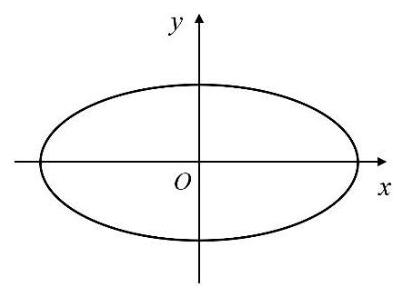
\includegraphics[max width=0.3\textwidth]{images/bo_d7fhnv491nqc73ercsbg_116_1127_1234_398_291_0.jpg}
\end{center}
\hspace*{3em} 

(1)求 \(\left| {MF}\right|\) 的最小值；

(2)当直线 \({l}_{1}\) 的斜率为 1 时,求 \(\bigtriangleup  {PQM}\) 面积的最大值及此时点 \(M\) 的坐标;

(3)若直线 \({PQ}\) 与直线 \({l}_{2} : x =  - 3\) 交于点 \(D\) ，点 \(D\) 不在 \(x\) 轴上， \(Q\) 关于原点的对称点为点 \(R\) ， 直线 \({PR}\) 与 \({l}_{2}\) 交于点 \(E\) ,求线段 \(\left| {DE}\right|\) 的取值范围.

【答案】( 1 ) \(3 - 2\sqrt{2}\) ；( 2 )最大值为 \(\frac{9 + 3\sqrt{10}}{10}\) ， \(M\) 坐标为 \(\left( {-\frac{9}{\sqrt{10}},\frac{1}{\sqrt{10}}}\right)\) ；( 3 ) \(\lbrack 4, + \infty )\)

【解析】(1) 由椭圆方程 \(\frac{{x}^{2}}{9} + {y}^{2} = 1\) 知, \({a}^{2} = 9,{b}^{2} = 1,{c}^{2} = {a}^{2} - {b}^{2} = 9 - 1 = 8\) ,所以右焦点 \(F\left( {2\sqrt{2},0}\right)\) ,设 \(M\left( {m,n}\right)\) ,则 \(\left| {MF}\right|  = \sqrt{{\left( m - 2\sqrt{2}\right) }^{2} + {n}^{2}}\) ,由 \(\frac{{m}^{2}}{9} + {n}^{2} = 1 \Rightarrow  {n}^{2} = 1 - \frac{{m}^{2}}{9}\) 代

入得: \(\left| {MF}\right|  = \sqrt{{\left( m - 2\sqrt{2}\right) }^{2} + {n}^{2}} = \sqrt{{\left( m - 2\sqrt{2}\right) }^{2} + 1 - \frac{{m}^{2}}{9}} \; = \sqrt{\frac{8{m}^{2}}{9} - 4\sqrt{2}m + 9} = \frac{\sqrt{8{m}^{2} - {36}\sqrt{2}m + {81}}}{3},\)

由于 \(m \in  \left\lbrack  {-3,3}\right\rbrack\) ,对称轴 \(m = \frac{9\sqrt{2}}{4} > 3\) ,

所以 \(\left| {MF}\right|  \geq  \frac{\sqrt{8 \times  9 - {36}\sqrt{2} \times  3 + {81}}}{3} = \sqrt{{17} - {12}\sqrt{2}} = \sqrt{9 - 2 \times  3 \times  \sqrt{8} + 8} = 3 - 2\sqrt{2}\) ,

即 \(\left| {MF}\right|\) 的最小值为 \(3 - 2\sqrt{2}\) ,此时点 \(M\) 为椭圆的右顶点.

(2)由直线 \({l}_{1}\) 的斜率为 1 且经过 \(P\left( {3,0}\right)\) ，可得直线方程 \(y = x - 3\) ，

与椭圆 \(\frac{{x}^{2}}{9} + {y}^{2} = 1\) 联立方程组,消元得: \(\frac{{x}^{2}}{9} + {\left( x - 3\right) }^{2} = 1 \Rightarrow  {10}{x}^{2} - {54x} + {72} = 0\) ,

解得 \(x = 3,x = \frac{12}{5}\) ,则代入 \(x = \frac{12}{5}\) 得: \(y = \frac{12}{5} - 3 =  - \frac{3}{5}\) ,所以 \(Q\left( {\frac{12}{5}, - \frac{3}{5}}\right)\) ,

则 \(\left| {PQ}\right|  = \sqrt{{\left( \frac{12}{5} - 3\right) }^{2} + {\left( -\frac{3}{5} - 0\right) }^{2}} = \frac{3\sqrt{2}}{5}\) ,

设平行于直线 \({l}_{1}\) 的直线方程为 \(y = x + t\) ,则与椭圆 \(\frac{{x}^{2}}{9} + {y}^{2} = 1\) 联立方程组,消元得:

\(\frac{{x}^{2}}{9} + {\left( x + t\right) }^{2} = 1 \Rightarrow  {10}{x}^{2} + {18tx} + 9{t}^{2} - 9 = 0\) ,当此直线与椭圆相切时,满足判别式为 0,

即 \(\Delta  = {18}^{2}{t}^{2} - 4 \times  {10} \times  \left( {9{t}^{2} - 9}\right)  = 0\) ,解得 \(t =  \pm  \sqrt{10}\) ,

根据数形结合可得 \(t = \sqrt{10}\) 时,满足切点 \(M\) 取到 \(\bigtriangleup  {PQM}\) 面积最大值，

此时方程为 \({10}{x}^{2} + {18}\sqrt{10}x + {81} = 0 \Rightarrow  {\left( \sqrt{10}x + 9\right) }^{2} = 0 \Rightarrow  x =  - \frac{9}{\sqrt{10}}\) ,

代入直线得 \(y =  - \frac{9}{\sqrt{10}} + \sqrt{10} = \frac{1}{\sqrt{10}}\) ,则 \(M\left( {-\frac{9}{\sqrt{10}},\frac{1}{\sqrt{10}}}\right)\) ,

由点 \(M\left( {-\frac{9}{\sqrt{10}},\frac{1}{\sqrt{10}}}\right)\) 到直线 \(y = x - 3\) 的距离公式得: \(d = \frac{\left| -\frac{9}{\sqrt{10}} - \frac{1}{\sqrt{10}} - 3\right| }{\sqrt{2}} = \frac{3 + \sqrt{10}}{\sqrt{2}},\)

所以 \(\bigtriangleup  {PQM}\) 面积的最大值为 \(S = \frac{1}{2} \times  \frac{3\sqrt{2}}{5} \times  \frac{3 + \sqrt{10}}{\sqrt{2}} = \frac{9 + 3\sqrt{10}}{10}\) ，

此时点 \(M\left( {-\frac{9}{\sqrt{10}},\frac{1}{\sqrt{10}}}\right)\) .

(3)设过点 \(P\left( {3,0}\right)\) 直线为: \(y = k\left( {x - 3}\right)\) ,与椭圆 \(\frac{{x}^{2}}{9} + {y}^{2} = 1\) 联立方程组，消元得: \(\frac{{x}^{2}}{9} + {k}^{2}{\left( x - 3\right) }^{2} = 1 \Rightarrow  \left( {1 + 9{k}^{2}}\right) {x}^{2} - {54}{k}^{2}x + {81}{k}^{2} - 9 = 0\) ,

由 \(\Delta  = {\left( -{54}{k}^{2}\right) }^{2} - 4\left( {1 + 9{k}^{2}}\right) \left( {{81}{k}^{2} - 9}\right)  = {36} > 0\) ,

再由于交点 \(D\) 不在 \(x\) 轴上,即 \(k \neq  0\) ,

设交点 \(Q\left( {{x}_{1},{y}_{1}}\right)\) ,则有 \({x}_{1} + 3 = \frac{{54}{k}^{2}}{1 + 9{k}^{2}} \Rightarrow  {x}_{1} = \frac{{27}{k}^{2} - 3}{1 + 9{k}^{2}}\) ,

代入 \({x}_{1} = \frac{{27}{k}^{2} - 3}{1 + 9{k}^{2}}\) 得: \({y}_{1} = k\left( {\frac{{27}{k}^{2} - 3}{1 + 9{k}^{2}} - 3}\right)  = \frac{-{6k}}{1 + 9{k}^{2}}\) ，

由于 \(Q\) 关于原点的对称点为点 \(R\) ,所以 \(R\left( {-\frac{{27}{k}^{2} - 3}{1 + 9{k}^{2}},\frac{6k}{1 + 9{k}^{2}}}\right)\) ,

则直线 \({PR}\) 方程为 \(y = \frac{\frac{6k}{1 + 9{k}^{2}}}{-\frac{{27}{k}^{2} - 3}{1 + 9{k}^{2}} - 3}\left( {x - 3}\right)\) ,与直线 \(x =  - 3\) 相交得:

\(E\) 点纵坐标为 \(y =  - 6\frac{\frac{6k}{1 + 9{k}^{2}}}{-\frac{{27}{k}^{2} - 3}{1 + 9{k}^{2}} - 3} = \frac{2}{3k}\) ,

而直线 \(y = k\left( {x - 3}\right)\) 与直线 \(x =  - 3\) 相交得:

\(D\) 点纵坐标为 \(y =  - {6k}\) ,

所以可得 \(\left| {DE}\right|  = \left| {\frac{2}{3k} + {6k}}\right|  = \left| \frac{2}{3k}\right|  + \left| {6k}\right|  \geq  2\sqrt{\left| \frac{2}{3k}\right|  \cdot  \left| {6k}\right| } = 4\)

当且仅当 \(\left| \frac{2}{3k}\right|  = \left| {6k}\right|\) ,即 \(k =  \pm  \frac{1}{3}\) 时, \(\left| {DE}\right|\) 取到最小值 4 .

即 \(\left| {DE}\right|\) 的取值范围是 \(\lbrack 4, + \infty )\) .

11.(2025 高三二模浦东 20)已知椭圆 \({C}_{1}\) 的方程为 \(\frac{{x}^{2}}{3} + {y}^{2} = 1\) ，右顶点为 \(A\) ，上顶点为 \(B\) ， 椭圆 \({C}_{2}\) 的中心位于坐标原点,两个椭圆的离心率相等.

(1)若椭圆 \({C}_{2}\) 的方程是 \(\frac{{x}^{2}}{{a}^{2}} + \frac{{y}^{2}}{2a} = 1\left( {a > 0}\right)\) ，焦点在 \(x\) 轴上，求 \(a\) 的值；

(2)设椭圆 \({C}_{2}\) 的焦点在 \(x\) 轴上，直线 \({AB}\) 与 \({C}_{2}\) 相交于点 \(C\text{ 、 }D\) ，若 \(\left| {CD}\right|  = 3\left| {AB}\right|\) ， 求 \({C}_{2}\) 的标准方程;

(3)设椭圆 \({C}_{2}\) 的焦点在 \(y\) 轴上，点 \(P\) 在 \({C}_{1}\) 上，点 \(Q\) 在 \({C}_{2}\) 上，若存在 \(\bigtriangleup  {APQ}\) 是等腰直角三角形,且 \(\left| {AP}\right|  = \left| {AQ}\right|\) ,求 \({C}_{2}\) 的长轴的取值范围.

【答案】(1) \(a = 6;\left( 2\right) \frac{{x}^{2}}{15} + \frac{{y}^{2}}{5} = 1;\left( 3\right) \left\lbrack  {2\sqrt{3},6\sqrt{3}}\right\rbrack\)

【解析】(1) 由题,椭圆 \({C}_{1}\) 的离心率为 \(\frac{\sqrt{6}}{3}\) ,椭圆 \({C}_{2}\) 的离心率为 \(\frac{\sqrt{{a}^{2} - {2a}}}{a}\) , \(\frac{\sqrt{6}}{3} = \frac{\sqrt{{a}^{2} - {2a}}}{a}\) ,解答 \(a = 6\) .

(2)由题， \(A\left( {\sqrt{3},0}\right)\) ， \(B\left( {0,1}\right)\) ， \(\therefore \left| {AB}\right|  = 2\) ，直线 \({AB}\) 的方程为 \(y =  - \frac{\sqrt{3}}{3}x + 1\) ， 设 \({C}_{2}\) 的方程为 \({x}^{2} + 3{y}^{2} = \lambda \left( {\lambda  > 0}\right) ,C\left( {{x}_{1},{y}_{1}}\right) ,D\left( {{x}_{2},{y}_{2}}\right)\) , 联立直线 \({AB}\) 与椭圆 \({C}_{2} : \left\{  \begin{array}{l} y =  - \frac{\sqrt{3}}{3}x + 1 \\  {x}^{2} + 3{y}^{2} = \lambda  \end{array}\right.\) ,代入整理得 \(2{x}^{2} - 2\sqrt{3}x + 3 - \lambda  = 0\) , 故 \(\left| {CD}\right|  = \sqrt{1 + {\left( -\frac{\sqrt{3}}{3}\right) }^{2}}\left| {{x}_{1} - {x}_{2}}\right|  = \frac{2}{\sqrt{3}}\frac{\sqrt{{12} - 8\left( {3 - \lambda }\right) }}{2} = 3\left| {AB}\right|  = 6\) , 即 \(\sqrt{{12} - 8\left( {3 - \lambda }\right) } = 6\sqrt{3}\) ,解得 \(\lambda  = {15}\) ,

\(\therefore {C}_{2}\) 的标准方程为 \(\frac{{x}^{2}}{15} + \frac{{y}^{2}}{5} = 1\) .

(3)由题,设 \({C}_{2}\) 的方程为 \(3{x}^{2} + {y}^{2} = \lambda \left( {\lambda  > 0}\right)\) ,

由题意, \({AP} \bot  {AQ}\) 且 \({\left| AP\right| }^{2} = {\left| AQ\right| }^{2}\) ,任取 \({C}_{1}\) 上一点 \(P\left( {{x}_{0},{y}_{0}}\right)\) (不与点 \(A\) 重合),

则 \({\left| AP\right| }^{2} = {\left( {x}_{0} - \sqrt{3}\right) }^{2} + {y}_{0}^{2},{k}_{AP} = \frac{{y}_{0}}{{x}_{n} - \sqrt{3}}\) ,

设 \(Q\left( {{x}_{Q},{y}_{Q}}\right)\) ,则 \({\left| AQ\right| }^{2} = {\left( {x}_{Q} - \sqrt{3}\right) }^{2} + {y}_{Q}^{2}\) ,

直线 \({AQ}\) 的方程为 \(x = \frac{1}{{k}_{AQ}}y + \sqrt{3} =  - {k}_{AP}y + \sqrt{3}\) ,故 \({x}_{Q} - \sqrt{3} =  - {k}_{AP}{y}_{Q}\) ,

带入得 \({\left| AQ\right| }^{2} = {\left( {x}_{Q} - \sqrt{3}\right) }^{2} + {y}_{Q}^{2} = \left( {{k}_{AP}^{2} + 1}\right) {y}_{Q}^{2} = \frac{{\left( {x}_{0} - \sqrt{3}\right) }^{2} + {y}_{0}^{2}}{{\left( {x}_{0} - \sqrt{3}\right) }^{2}}{y}_{Q}^{2} = \frac{{\left| AP\right| }^{2}}{{\left( {x}_{0} - \sqrt{3}\right) }^{2}}{y}_{Q}^{2}\) ,

\(\because {\left| AP\right| }^{2} = {\left| AQ\right| }^{2}\) ,解得 \({y}_{Q}^{2} = {\left( {x}_{0} - \sqrt{3}\right) }^{2}\) ,由对称性,不妨设 \({y}_{Q} = {x}_{0} - \sqrt{3}\) ,

代回直线 \({AQ}\) 方程可解得 \(Q\left( {\sqrt{3} - {y}_{0},{x}_{0} - \sqrt{3}}\right)\) ,而点 \(Q\) 位于 \({C}_{2}\) 上,

\(\therefore \lambda  = 3{\left( \sqrt{3} - {y}_{0}\right) }^{2} + {\left( {x}_{0} - \sqrt{3}\right) }^{2} = 3\left( {{y}_{0}{}^{2} - 2\sqrt{3}{y}_{0} + 3}\right)  + {x}_{0}{}^{2} - 2\sqrt{3}{x}_{0} + 3\)

\(= \left( {{x}_{0}^{2} + 3{y}_{0}^{2}}\right)  + {12} - 2\sqrt{3}\left( {{x}_{0} + 3{y}_{0}}\right) ,\)

\(P\left( {{x}_{0},{y}_{0}}\right)\) 为 \({C}_{1}\) 上任一点, \(\therefore {x}_{0}^{2} + 3{y}_{0}^{2} = 3\) 为定值,化简得 \(\lambda  = {15} - 2\sqrt{3}\left( {{x}_{0} + 3{y}_{0}}\right)\) ,

设 \({x}_{0} + 3{y}_{0} = b,P\left( {{x}_{0},{y}_{0}}\right)\) 为 \({C}_{1}\) 上任一点,即 \(\left\{  \begin{array}{l} \frac{{x}_{0}^{2}}{3} + {y}_{0}^{2} = 1 \\  {x}_{0} + 3{y}_{0} = b \end{array}\right.\) 有解,

整理得 \({12}{y}_{0}^{2} - {6b}{y}_{0} + {b}^{2} - 3 = 0,\Delta  = {36}{b}^{2} - {48}\left( {{b}^{2} - 3}\right)  = {12}\left( {{12} - {b}^{2}}\right)  \geq  0\) ,

解得 \(b \in  \left\lbrack  {-2\sqrt{3},2\sqrt{3}}\right\rbrack  ,\therefore \lambda  = {15} - 2\sqrt{3}b \in  \left\lbrack  {3,{27}}\right\rbrack\) ,

故 \({C}_{2}\) 的长轴长 \(2\sqrt{\lambda } \in  \left\lbrack  {2\sqrt{3},6\sqrt{3}}\right\rbrack\) .

\section*{四、双曲线的综合}

1.(2025 高三二模徐汇 10)已知双曲线 \(\frac{{x}^{2}}{{a}^{2}} - \frac{{y}^{2}}{{b}^{2}} = 1\left( {a > 0,b > 0}\right)\) 的左焦点为 \({F}_{1}\) ，右焦点为 \({F}_{2}\) . 若双曲线的右支上存在一点 \(P\) ,使得直线 \(P{F}_{1}\) 与以双曲线的实轴为直径的圆相切,切点为线段 \(P{F}_{1}\) 的中点，则该双曲线的离心率为\_\_\_\_\_.

【答案】 \(\sqrt{5}\)

【解析】设切点为 \(A\) ,因为 \({OA} = a,O{F}_{1} = c,\therefore A{F}_{1} = \sqrt{{c}^{2} - {a}^{2}} = b,\therefore P{F}_{1} = {2b}\) ,

又 \(P{F}_{1} - P{F}_{2} = {2a},\therefore P{F}_{2} = {2b} - {2a}\) ,

则 \(P{F}_{1} - P{F}_{2} = {2a},\therefore P{F}_{2} = {2b} - {2a}\) ,

\(\cos \left( {A{F}_{1}{F}_{2}}\right)  = \frac{b}{c} = \frac{P{F}_{1}^{2} + {F}_{1}{F}_{2}^{2} - P{F}_{2}^{2}}{{2P}{F}_{1} \cdot  {F}_{1}{F}_{2}} = \frac{4{b}^{2} + 4{c}^{2} - {\left( 2b - 2a\right) }^{2}}{2 \cdot  {2b} \cdot  {2c}},\)

化简可得 \(b = {2a},\therefore e = \frac{c}{a} = \frac{\sqrt{{a}^{2} + {\left( 2a\right) }^{2}}}{a} = \sqrt{5}\) .

\begin{center}
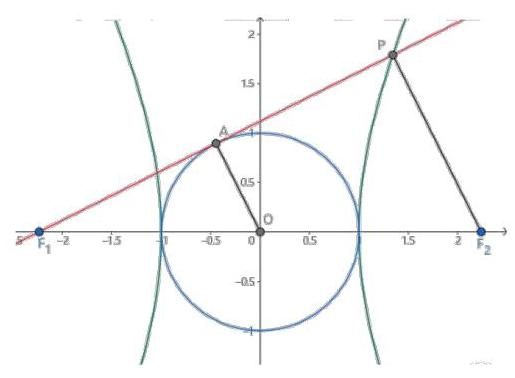
\includegraphics[max width=0.4\textwidth]{images/bo_d7fhnv491nqc73ercsbg_121_234_898_515_378_0.jpg}
\end{center}
\hspace*{3em} 

2.(2025 高三二模崇明 11)已知双曲线 \({x}^{2} - \frac{{y}^{2}}{{b}^{2}} = 1\left( {b > 0}\right)\) 的左，右焦点为 \({F}_{1},{F}_{2}\) . 以 \(O\) 为顶点， \({F}_{2}\) 为焦点作抛物线交双曲线于 \(P\) ，且 \(\angle P{F}_{1}{F}_{2} = {45}^{ \circ  }\) ，则 \({b}^{2} =\) \_\_\_\_\_.

【答案】 \(2 + 2\sqrt{2}\)

【解析】过 \({F}_{1}\) 作 \(x\) 轴的垂线,过 \(P\) 作垂线,垂足为 \(A\) ,如图所示,

\(\because \angle P{F}_{1}{F}_{2} = {45}^{ \circ  }\) ,则 \(\angle {F}_{1}{PA} = {45}^{ \circ  }\) ,

由抛物线的定义可知 \(P{F}_{2} = {PA},\therefore P{F}_{1} = \sqrt{2}P{F}_{2},\therefore P{F}_{1} - P{F}_{2} = \left( {\sqrt{2} - 1}\right) P{F}_{2} = {2a} = 2\) ,

\(\therefore P{F}_{2} = 2 + 2\sqrt{2},P{F}_{1} = 4 + 2\sqrt{2}\) ,

由余弦定理可得

\(\cos \angle P{F}_{1}{F}_{2} = \cos {45}^{ \circ  } = \frac{\sqrt{2}}{2} = \frac{P{F}_{1}^{2} + {F}_{1}{F}_{2}^{2} - P{F}_{2}^{2}}{{2P}{F}_{1} \cdot  {F}_{1}{F}_{2}} = \frac{{\left( 4 + 2\sqrt{2}\right) }^{2} + 4{c}^{2} - {\left( 2 + 2\sqrt{2}\right) }^{2}}{2 \times  \left( {4 + 2\sqrt{2}}\right)  \times  {2c}},\) 解得 \(c = 1 + \sqrt{2},\therefore {b}^{2} = {\left( 1 + \sqrt{2}\right) }^{2} - 1 = 2 + 2\sqrt{2}\) .

\begin{center}
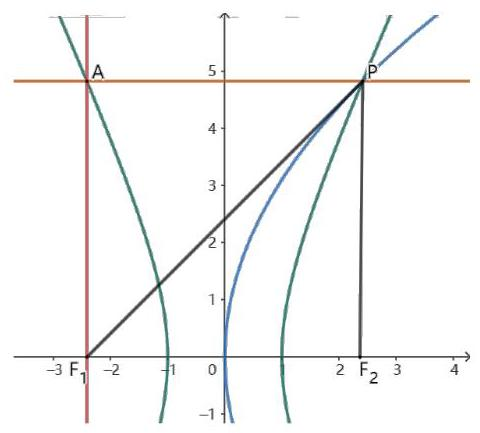
\includegraphics[max width=0.4\textwidth]{images/bo_d7fhnv491nqc73ercsbg_122_236_285_480_433_0.jpg}
\end{center}
\hspace*{3em} 

3. (2025 高三二模普陀 15)设 \(a > 0,b > 0\) ，点 \(M\left( {{x}_{0},{y}_{0}}\right) ,O\) 是坐标原点， \(\left| {OM}\right|  = a\) ， \(F\) 是双曲线 \(\Gamma  : \frac{{x}^{2}}{{a}^{2}} - \frac{{y}^{2}}{{b}^{2}} = 1\) 的左焦点,若直线 \(l : {x}_{0}x + {y}_{0}y = {a}^{2}\) 经过点 \(F\) ,且与双曲线 \(\Gamma\) 的右支在第一象限内交于 \(P\) 点，则双曲线 \(\Gamma\) 的离心率的一个可能的值为( )

A. \(\frac{\sqrt{5}}{2}\) B. \(\frac{\sqrt{6}}{2}\) C. \(\frac{\sqrt{7}}{2}\) D. \(\frac{\sqrt{11}}{2}\)

【答案】D

【解析】由题意,点 \(M\) 的轨迹为 \({x}^{2} + {y}^{2} = {a}^{2}\) ,可知直线 \(l : {x}_{0}x + {y}_{0}y = {a}^{2}\) 与点 \(M\) 的轨迹有交点,又直线 \(l : {x}_{0}x + {y}_{0}y = {a}^{2}\) 经过点 \(F\) ,不妨重新设直线 \(l : y = k\left( {x + c}\right)\) ,经过双曲线的左焦点 \(F\) 且与圆 \({x}^{2} + {y}^{2} = {a}^{2}\) 有交点，

则有 \(\frac{\left| ck\right| }{\sqrt{1 + {k}^{2}}} \leq  a\) ,可得 \(k \leq  \frac{a}{b}\) ,

又直线 \(l\) 与双曲线的右支在第一象限内交于 \(P\) 点,可知直线 \(l\) 的斜率小于渐近线的斜率,

所以有 \(\frac{a}{b} < \frac{b}{a} \Rightarrow  {a}^{2} < {b}^{2}\) ,

则离心率 \(e = \frac{c}{a} = \sqrt{\frac{{c}^{2}}{{a}^{2}}} = \sqrt{\frac{{a}^{2} + {b}^{2}}{{a}^{2}}} = \sqrt{1 + \frac{{b}^{2}}{{a}^{2}}} > \sqrt{2}\) ,故选 D.

4. (2025 高三二模长宁 20)已知双曲线 \(\Gamma  : \frac{{x}^{2}}{{a}^{2}} - \frac{{y}^{2}}{{b}^{2}} = 1\) 的左、右焦点分别为 \({F}_{1},{F}_{2}\) ，点 \(A\) 是其左顶点,点 \(P\) 是双曲线上一点,且位于第一象限,若双曲线 \(\Gamma\) 的离心率 \(e = 2,b = 2\sqrt{3}\) .

(1)求双曲线 \(\Gamma\) 的方程；

(2)若三角形 \({AP}{F}_{2}\) 是等腰三角形,求点 \(P\) 的坐标；

(3)直线 \(P{F}_{2}\) 不垂直于 \(x\) 轴,且与双曲线的另一个交点为 \(Q\) ,若 \(\angle P{F}_{1}Q\) 是锐角,求直线 \(P{F}_{2}\) 的斜率的取值范围.

【答案】(1) \(\frac{{x}^{2}}{4} - \frac{{y}^{2}}{12} = 1\) ; (2) \(P\left( {\frac{-1 + 3\sqrt{5}}{2},\sqrt{\frac{{45} - 9\sqrt{5}}{2}}}\right)\) ;

(3) \(\left( {-\infty , - \sqrt{3}}\right)  \cup  \left( {-\frac{3\sqrt{7}}{7},0}\right)  \cup  \left( {\sqrt{3}, + \infty }\right)\)

【解析】(1) \(e = \frac{c}{a} = 2\) ,所以

\(c = {2a},\) .2 分

由 \({c}^{2} = {a}^{2} + {b}^{2}\) ,可得 \(c = 4\) ,

\(a = 2\) , .2 分

所以双曲线 \(\Gamma\) 的方程为 \(\frac{{x}^{2}}{4} - \frac{{y}^{2}}{12} = 1\)

(2)若 \({AP} = {P{F}_{2}}\) ，则 \(P\) 在直线 \(x = 1\) 上，

直线 \(x = 1\) 与双曲线不相交,所以不存在满足条件的点 \(P\) , .2 分

设 \(P\left( {x,y}\right)\) ,若 \({AP} = A{F}_{2} = 6\) ,则 \(\left\{  \begin{array}{l} {\left( x + 2\right) }^{2} + {y}^{2} = {36} \\  3{x}^{2} - {y}^{2} = {12} \end{array}\right.\) ,

得 \(P\left( {\frac{-1 + 3\sqrt{5}}{2},\sqrt{\frac{{45} - 9\sqrt{5}}{2}}}\right)\) , .2 分

若 \(P{F}_{2} = A{F}_{2} = 6\) ,则 \(\left\{  \begin{array}{l} {\left( x - 4\right) }^{2} + {y}^{2} = {36} \\  3{x}^{2} - {y}^{2} = {12} \end{array}\right.\) ,得 \(P\left( {4,6}\right)\) , .2分

综上,点 \(P\) 的坐标是 \(P\left( {\frac{-1 + 3\sqrt{5}}{2},\sqrt{\frac{{45} - 9\sqrt{5}}{2}}}\right) \text{ 、 }P\left( {4,6}\right)\) .

(3)设直线 \({PQ}\) 的解析式为 \(y = k\left( {x - 4}\right) ,P\left( {{x}_{1},{y}_{1}}\right) ,Q\left( {{x}_{2},{y}_{2}}\right)\)

由 \(\left\{  \begin{array}{l} y = k\left( {x - 4}\right) \\  {x}^{2} - 3{y}^{2} = {12} \end{array}\right.\) ,

可得 \(\left( {3 - {k}^{2}}\right) {x}^{2} + 8{k}^{2}x - {16}{k}^{2} - {12} = 0\) .2 分

\(\Delta  = {144}{k}^{2} + {144} > 0\) ,直线 \({PQ}\) 与双曲线有两个交点,所以 \({k}^{2} \neq  3\) ,

\({x}_{1} + {x}_{2} = \frac{-8{k}^{2}}{3 - {k}^{2}},\;{x}_{1}{x}_{2} = \frac{-{16}{k}^{2} - {12}}{3 - {k}^{2}},\) .2 分

因为点 \(P\) 在第一象限,所以 \(k > \sqrt{3}\) 或 \(k < 0\)

\(\overrightarrow{P{F}_{1}} \cdot  \overrightarrow{Q{F}_{1}} > 0\) 可得 \(\frac{7{k}^{2} - 9}{{k}^{2} - 3} > 0\) 2 分

得 \({k}^{2} > 3\) 或 \(0 < {k}^{2} < \frac{9}{7}\) ,

所以,直线 \({PQ}\) 斜率的取值范围是 \(\left( {-\infty , - \sqrt{3}}\right)  \cup  \left( {-\frac{3\sqrt{7}}{7},0}\right)  \cup  \left( {\sqrt{3}, + \infty }\right)\) . .2 分

5.(2025 高三二模杨浦 20)已知双曲线 \(\Gamma\) 的标准方程为 \({x}^{2} - \frac{{y}^{2}}{2} = 1\) ，点 \(P\) 是双曲线 \(\Gamma\) 右支上的一个动点.

\begin{center}
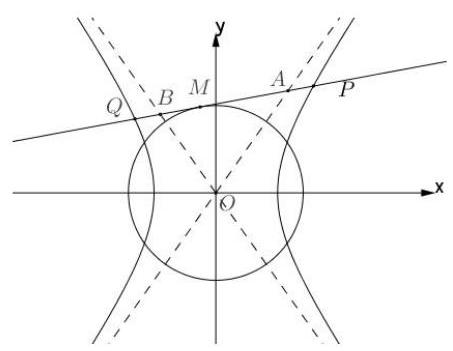
\includegraphics[max width=0.3\textwidth]{images/bo_d7fhnv491nqc73ercsbg_124_984_909_453_351_0.jpg}
\end{center}
\hspace*{3em} 

第 20 题图

(1)求双曲线 \(\Gamma\) 的焦点坐标和渐近线方程;

(2)过点 \(P\) 分别向两条渐近线作垂线，垂足为点 \({P}_{1}\text{ 、 }{P}_{2}\) ， 求 \(\overrightarrow{P{P}_{1}} \cdot  \overrightarrow{P{P}_{2}}\) 的值；

(3)若 \(\left| {OP}\right|  > \sqrt{2}\) ，如图，过 \(P\) 作 \(\odot  O : {x}^{2} + {y}^{2} = 2\) 的切线 \(l\) ， 切点为 \(M\) ,交双曲线 \(\Gamma\) 的左支于点 \(Q\) ,分别交两条渐近线于点 \(A\) 、 \(B\) . 设 \(\left| {PQ}\right|  = \lambda \left| {AB}\right|\) ,求实数 \(\lambda\) 的取值范围.

【答案】(1) 焦点坐标为 \(\left( {\sqrt{3},0}\right)\) 和 \(\left( {-\sqrt{3},0}\right)\) ,渐近线方程为 \(y = \sqrt{2}x\) 和 \(y =  - \sqrt{2}x;\left( 2\right) \frac{2}{9};\left( 3\right) \; \lambda  \in  \left( {1,\sqrt{2}}\right\rbrack\)

【解析】(1) 双曲线 \(\Gamma\) 的焦点坐标为 \(\left( {\sqrt{3},0}\right)\) 和 \(\left( {-\sqrt{3},0}\right)\) ,渐近线方程为 \(y = \sqrt{2}x\) 和 \(y =  - \sqrt{2}x\ldots \ldots {.4}\)

(2)设 \(P\left( {{x}_{0},{y}_{0}}\right)\) ，则 \({x}_{0}^{2} - \frac{{y}_{0}^{2}}{2} = 1\) ， .5

不妨设 \(\overrightarrow{P{P}_{1}}\) 垂直于直线 \(y = \sqrt{2}x,\overrightarrow{P{P}_{2}}\) 垂直于直线 \(y =  - \sqrt{2}x\) ,

则 \(\overrightarrow{{n}_{1}} = \left( {-\sqrt{2},1}\right)\) 是与 \(\overrightarrow{P{P}_{1}}\) 同向的一个向量, \(\overrightarrow{{n}_{2}} = \left( {-\sqrt{2}, - 1}\right)\) 是与 \(\overrightarrow{P{P}_{2}}\) 同向的一个向量,

可得 \(\cos \left\langle  {\overrightarrow{P{P}_{1}},\overrightarrow{P{P}_{2}}}\right\rangle   = \cos \left( {\overrightarrow{{n}_{1}},\overrightarrow{{n}_{2}}}\right)  = \frac{{\left( -\sqrt{2}\right) }^{2} - 1}{\sqrt{1 + 2} \cdot  \sqrt{1 + 2}} = \frac{1}{3}\) , .7

\(\left| \overrightarrow{P{P}_{1}}\right|  = \frac{\left| \sqrt{2}{x}_{0} - {y}_{0}\right| }{\sqrt{2 + 1}} = \frac{\left| \sqrt{2}{x}_{0} - {y}_{0}\right| }{\sqrt{3}},\left| \overrightarrow{P{P}_{2}}\right|  = \frac{\left| \sqrt{2}{x}_{0} + {y}_{0}\right| }{\sqrt{2 + 1}} = \frac{\left| \sqrt{2}{x}_{0} + {y}_{0}\right| }{\sqrt{3}},\) .9

\(\overrightarrow{P{P}_{1}} \cdot  \overrightarrow{P{P}_{2}} = \left| \overrightarrow{P{P}_{1}}\right|  \cdot  \left| \overrightarrow{P{P}_{2}}\right|  \cdot  \cos \left\langle  {\overrightarrow{P{P}_{1}},\overrightarrow{P{P}_{2}}}\right\rangle   = \frac{\left| 2{x}_{0}^{2} - {y}_{0}^{2}\right| }{3} \cdot  \frac{1}{3} = \frac{2}{9}\) . .10

(3)设 \(M\left( {{x}_{0},{y}_{0}}\right)\) ，则 \({x}_{0}^{2} + {y}_{0}^{2} = 2\) 且 \({x}_{0} \in  \left( {-\frac{2\sqrt{3}}{3},\frac{2\sqrt{3}}{3}}\right)\) ， .12

由 \(\overrightarrow{OM} = \left( {{x}_{0},{y}_{0}}\right)\) ,则切线 \(l\) 的方程为 \({x}_{0}\left( {x - {x}_{0}}\right)  + {y}_{0}\left( {y - {y}_{0}}\right)  = 0\) ,化简得 \({x}_{0}x + {y}_{0}y = 2\) ,

\(\left\{  \begin{array}{l} {x}_{0}x + {y}_{0}y = 2 \\  {x}^{2} - \frac{{y}^{2}}{2} = 1 \end{array}\right.\) 消去 \(y\) 得 \(\left( {{x}_{0}^{2} - 2{y}_{0}^{2}}\right) {x}^{2} - 4{x}_{0}x + 2{y}_{0}^{2} + 4 = 0\) , .14

因为 \({x}_{0}^{2} + {y}_{0}^{2} = 2\) ,整理得 \(\left( {3{x}_{0}^{2} - 4}\right) {x}^{2} - 4{x}_{0}x + 8 - 2{x}_{0}^{2} = 0\)

因为 \({x}_{0} \in  \left( {-\frac{2\sqrt{3}}{3},\frac{2\sqrt{3}}{3}}\right)\) ,可得 \(3{x}_{0}^{2} - 4 < 0\) ,

\(\Delta  = {\left( -4{x}_{0}\right) }^{2} - 4\left( {3{x}_{0}^{2} - 4}\right) \left( {8 - 2{x}_{0}^{2}}\right)  = 8\left( {3{x}_{0}^{2} - 8}\right) \left( {{x}_{0}^{2} - 2}\right)  > 0.\)

设 \(P\left( {{x}_{1},{y}_{1}}\right) \text{ 、 }Q\left( {{x}_{2},{y}_{2}}\right)\) ,则 \({x}_{1} + {x}_{2} = \frac{4{x}_{0}}{3{x}_{0}^{2} - 4}\text{ 、 }{x}_{1}{x}_{2} = \frac{8 - 2{x}_{0}^{2}}{3{x}_{0}^{2} - 4}\) ,

\(\left| {PQ}\right|  = \sqrt{1 + {\left( -\frac{{x}_{0}}{{y}_{0}}\right) }^{2}}\left| {{x}_{1} - {x}_{2}}\right|  = \sqrt{\frac{{y}_{0}^{2} + {x}_{0}^{2}}{{y}_{0}^{2}}} \cdot  \sqrt{{\left( {x}_{1} + {x}_{2}\right) }^{2} - 4{x}_{1}{x}_{2}} = \frac{\sqrt{2}}{\left| {y}_{0}\right| } \cdot  \frac{\sqrt{8\left( {3{x}_{0}^{2} - 8}\right) \left( {-{y}_{0}^{2}}\right) }}{4 - 3{x}_{0}^{2}} = \frac{4\sqrt{8 - 3{x}_{0}^{2}}}{4 - 3{x}_{0}^{2}},\)

渐近线方程为 \(y = \sqrt{2}x\) 和 \(y =  - \sqrt{2}x\) ,

\(\left\{  {\begin{array}{l} {x}_{0}x + {y}_{0}y = 2 \\  y = \sqrt{2}x \end{array}\text{ 得 }x = \frac{2}{{x}_{0} + \sqrt{2}{y}_{0}};\left\{  {\begin{array}{l} {x}_{0}x + {y}_{0}y = 2 \\  y =  - \sqrt{2}x \end{array}\text{ 得 }x = \frac{2}{{x}_{0} - \sqrt{2}{y}_{0}},}\right. }\right.\)

\(\left| {AB}\right|  = \sqrt{1 + {\left( -\frac{{x}_{0}}{{y}_{0}}\right) }^{2}}\left| {\frac{2}{{x}_{0} + \sqrt{2}{y}_{0}} - \frac{2}{{x}_{0} - \sqrt{2}{y}_{0}}}\right|  = \frac{\sqrt{2}}{\left| {y}_{0}\right| } \cdot  \frac{\left| 4\sqrt{2}{y}_{0}\right| }{\left| {x}_{0}^{2} - 2{y}_{0}^{2}\right| } = \frac{8}{4 - 3{x}_{0}^{2}},\) .16 \(\lambda  = \frac{\left| PQ\right| }{\left| AB\right| } = \frac{\frac{4\sqrt{8 - 3{x}_{0}^{2}}}{4 - 3{x}_{0}^{2}}}{\frac{8}{4 - 3{x}_{0}^{2}}} = \frac{\sqrt{8 - 3{x}_{0}^{2}}}{2},{x}_{0} \in  \left( {-\frac{2\sqrt{3}}{3},\frac{2\sqrt{3}}{3}}\right)\) ,则 \({x}_{0}^{2} \in  \left\lbrack  {0,\frac{4}{3}}\right) ,\lambda  \in  (1,\sqrt{2}\rbrack\) .18

6. (2025 高三二模虹口 20)已知点 \({F}_{1}\) 和 \({F}_{2}\) 是双曲线 \(C : \frac{{x}^{2}}{{a}^{2}} - {y}^{2} = 1\left( {a > 0}\right)\) 的左、右焦点.

(1)若 \(y = x\) 是双曲线 \(C\) 的一条渐近线，求 \(C\) 的离心率；

(2)当 \(a = \sqrt{2}\) 时，若双曲线 \(C\) 上存在一点 \(P\) 满足 \(\left| {P{F}_{1}}\right|  + \left| {P{F}_{2}}\right|  = 4\) ，求 \({\Delta P}{F}_{1}{F}_{2}\) 的面积；

(3)若在双曲线 \(C\) 上分别存在两点 \(A\) 和 \(B\) ，点 \(A\) 在第一象限、点 \(B\) 在第二象限，使得四边形 \({F}_{1}{BA}{F}_{2}\) 的面积为 \(2\sqrt{{a}^{2} + 1}\) ，且存在实数 \(\lambda\) 使 \(\overrightarrow{{F}_{2}A} = \lambda \overrightarrow{{F}_{1}B}\) ，求实数 \(a\) 的取值范围.

【答案】(1) \(\sqrt{2}\) ；(2) 1 ;(3) \(a \geq  1\)

【解析】(1)双曲线 \(C\) 的渐近线为 \(y =  \pm  \frac{1}{a}x\) ,

由于 \(y = x\) 是双曲线 \(C\) 的一条渐近线,故 \(a = 1\) . .2 分

所以 \({c}^{2} = {a}^{2} + 1 = 2\) ,故 \(e = \frac{c}{a} = \sqrt{2}\) . .4 分

(2)由于点 \(P\) 满足 \(\left| {P{F}_{1}}\right|  + \left| {P{F}_{2}}\right|  = 4 > 2\sqrt{2}\) ，所以点 \(P\) 落在椭圆 \(\frac{{x}^{2}}{4} + {y}^{2} = 1\) 上....6分设 \(P\left( {x,y}\right)\) ,则 \(\left\{  \begin{array}{l} \frac{{x}^{2}}{2} - {y}^{2} = 1, \\  \frac{{x}^{2}}{4} + {y}^{2} = 1 \end{array}\right.\) 解得 \({y}^{2} = \frac{1}{3}\) . .8 分由于 \(\left| {{F}_{1}{F}_{2}}\right|  = 2\sqrt{3}\) ,所以 \({\Delta P}{F}_{1}{F}_{2}\) 的面积 \(S = \frac{1}{2}\;2\sqrt{3}\frac{\sqrt{3}}{3} = 1\) . .10 分

(3)由于存在实数 \(\lambda\) 使 \(\overrightarrow{{F}_{2}A} = \lambda \overrightarrow{{F}_{1}B}\) ,故 \({F}_{2}A//{F}_{1}B\) .

延长 \(A{F}_{2}\) 交双曲线 \(C\) 于点 \({B}^{\prime }\) ，由双曲线的对称性，可得 \({B}^{\prime }\) 与 \(B\) 关于原点对称，故四边形 \({F}_{1}{BA}{F}_{2}\) 的面积与三角形 \({BA}{B}^{\prime }\) 的面积相等. .12 分

设 \(A{B}^{\prime }\) 的直线方程为 \(x = {ty} + c\) ,其中 \(c = \sqrt{{a}^{2} + 1}\) ,设 \(A\left( {{x}_{1},{y}_{1}}\right) ,{B}^{\prime }\left( {{x}_{2},{y}_{2}}\right)\) .

\(\left\{  \begin{array}{l} x = {ty} + c, \\  {x}^{2} - {a}^{2}{y}^{2} = {a}^{2} \end{array}\right.\) 化简得 \(\left( {{t}^{2} - {a}^{2}}\right) {y}^{2} + {2tcy} + {c}^{2} - {a}^{2} = 0\) ,故 \({y}_{1} + {y}_{2} =  - \frac{2tc}{{t}^{2} - {a}^{2}}\) ,

\({y}_{1}{y}_{2} = \frac{{c}^{2} - {a}^{2}}{{t}^{2} - {a}^{2}} = \frac{1}{{t}^{2} - {a}^{2}}.\)

由于 \(A\left( {{x}_{1},{y}_{1}}\right)\) 在第一象限, \({B}^{\prime }\left( {{x}_{2},{y}_{2}}\right)\) 在第四象限,故 \({y}_{1}{y}_{2} = \frac{{c}^{2} - {a}^{2}}{{t}^{2} - {a}^{2}} = \frac{1}{{t}^{2} - {a}^{2}} < 0\) ,解得 \({t}^{2} \in  \left\lbrack  {0,{a}^{2}}\right)\) . .14 分

所以三角形 \({BA}{B}^{\prime }\) 的面积 \(S = \frac{1}{2}\left| {{F}_{1}{F}_{2}}\right|  \cdot  \left| {{y}_{1} - {y}_{2}}\right|  = \frac{2ac}{{a}^{2} - {t}^{2}}\sqrt{{t}^{2} + 1}\) . .16 分由 \(S = 2\sqrt{{a}^{2} + 1} = {2c}\) ,故 \(\frac{2ac}{{a}^{2} - {t}^{2}}\sqrt{{t}^{2} + 1} = {2c}\) 对 \({t}^{2} \in  \left\lbrack  {0,{a}^{2}}\right)\) 有解.

化简得 \({t}^{4} - 3{a}^{2}{t}^{2} + {a}^{4} - {a}^{2} = 0\) 对 \({t}^{2} \in  \left\lbrack  {0,{a}^{2}}\right)\) 有解.

设 \(m = {t}^{2} \in  \left\lbrack  {0,{a}^{2}}\right)\) ,则 \({m}^{2} - 3{a}^{2}m + {a}^{4} - {a}^{2} = 0\) 对 \(m \in  \left\lbrack  {0,{a}^{2}}\right)\) 有解. 设

\(f\left( m\right)  = {m}^{2} - 3{a}^{2}m + {a}^{4} - {a}^{2}\) ,可得 \(f\left( {a}^{2}\right)  = {a}^{4} - 3{a}^{4} + {a}^{4} - {a}^{2} =  - {a}^{4} - {a}^{2} < 0\) 恒成立,

故 \(f\left( 0\right)  \geq  0\) ,即 \({a}^{4} - {a}^{2} \geq  0\) ,由 \(a > 0\) ,解得 \(a \geq  1\) . 1.8 分

7.(2025 高三二模宝山 20)已知双曲线 \(C : {x}^{2} - \frac{{y}^{2}}{3} = 1,{F}_{1}\text{ 、 }{F}_{2}\) 分别是其左、右焦点,直线 \(l\) 与双曲线 \(C\) 的右支交于 \(A\text{ 、 }B\) 两点.

\begin{center}
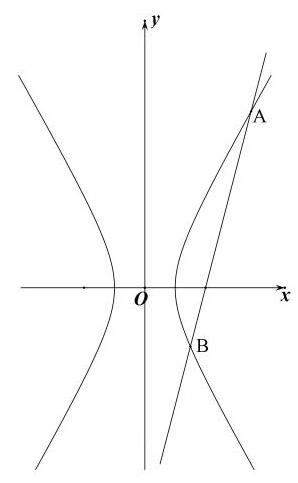
\includegraphics[max width=0.2\textwidth]{images/bo_d7fhnv491nqc73ercsbg_127_1199_659_298_483_0.jpg}
\end{center}
\hspace*{3em} 

(1)当直线 \(l\) 过点 \({F}_{2}\) ，且 \(\left| {AB}\right|  = 6\) 时，求 \(\bigtriangleup  {AB}{F}_{1}\) 的周长；

(2)已知点 \(N\left( {-2,3}\right)\) ，若直线 \({AN}\) 、 \({BN}\) 的斜率之和为\_\_\_\_\_，且 \(\tan \angle {ANB} = \frac{4}{3}\) ， 当 \({AN}\) 、 \({BN}\) 分别与 \(y\) 轴交于点 \(R\) 、 \(S\) 时，求 \(\bigtriangleup  {RSN}\) 的面积；

(3)已知直线 \(l\) 过点 \({F}_{2},P\) 是双曲线 \(C\) 上一点且位于第一象限，且满足 \(\overrightarrow{OQ} = 2\overrightarrow{OP}\) 的点 \(Q\) 在线段 \({AB}\) 上,若 \(\overrightarrow{AB} = 2\overrightarrow{Q{F}_{2}}\) ,求点 \(P\) 的坐标.

【答案】( 1 )16 ;( 2 )2 ; ( 3 ) \(\left( {\frac{3}{2},\frac{\sqrt{15}}{2}}\right)\)

【解析】(1) 根据双曲线定义得: \(\left| {A{F}_{1}}\right|  - \left| {A{F}_{2}}\right|  = 2,\left| {B{F}_{1}}\right|  - \left| {B{F}_{2}}\right|  = 2\) .2 分两式相加得 \(\left| {A{F}_{1}}\right|  + \left| {B{F}_{1}}\right|  - \left( {\left| {A{F}_{2}}\right|  + \left| {B{F}_{2}}\right| }\right)  = 4\) ,

即 \(\left| {A{F}_{1}}\right|  + \left| {B{F}_{1}}\right|  - \left| {AB}\right|  = 4\) ,

由已知 \(\left| {AB}\right|  = 6\) 得 \(\left| {A{F}_{1}}\right|  + \left| {B{F}_{1}}\right|  = {10}\) ，

所以 \({\Delta AB}{F}_{1}\) 的周长为 16 .4 分

(2)设直线 \({AN}\text{ 、 }{BN}\) 的倾斜角分别为 \(\alpha \text{ 、 }\beta\) ，

由已知 \({k}_{AN} + {k}_{BN} = 0\) 得 \(\alpha  + \beta  = \pi\) , .5 分

不妨设 \(0 < \alpha  < \frac{\pi }{2} < \beta  < \pi\) ,

则 \(\angle {ANB} = {2\alpha }\) ,

则 \(\tan \angle {ANB} = \tan {2\alpha } = \frac{4}{3}\) 可求得 \(\tan \alpha  = \frac{1}{2}\) 或-2(舍), \(\tan \beta  =  - \frac{1}{2}\) . .7 分

所以直线 \({AN} : y - 3 = \frac{1}{2}\left( {x + 2}\right)\) 解得 \(R\left( {0,4}\right)\) ,

直线 \({BN} : y - 3 =  - \frac{1}{2}\left( {x + 2}\right)\) 解得 \(S\left( {0,2}\right)\) , 所以 \({\Delta RSN}\) 的面积为 \(\frac{1}{2}\left| {RS}\right|  \cdot  \left| {x}_{N}\right|  = \frac{1}{2} \times  2 \times  2 = 2\) .9 分

(3)设 \(P\left( {{x}_{0},{y}_{0}}\right) ,\left( {{x}_{0} > 0,{y}_{0} > 0}\right)\) ，由 \(\overrightarrow{OQ} = 2\overrightarrow{OP}\) 知 \(Q\left( {2{x}_{0},2{y}_{0}}\right)\) ，

若直线 \(l\) 斜率不存在,则 \(l : x = 2\) ,此时 \(P\left( {1,0}\right) ,Q\left( {2,0}\right)\) 与点 \({F}_{2}\left( {2,0}\right)\) 重合,不符题意,舍.

.10 分

设直线 \(l\) 方程为: \(y = k\left( {x - 2}\right)\) ,

与双曲线 \(C : {x}^{2} - \frac{{y}^{2}}{3} = 1\) 联立化简得 \(\left( {{k}^{2} - 3}\right) {x}^{2} - 4{k}^{2}x + 4{k}^{2} + 3 = 0\) ,

\({k}^{2} - 3 \neq  0,\Delta  > 0\) 显然成立,

设交点 \(A\left( {{x}_{1},{y}_{1}}\right) \text{ 、 }B\left( {{x}_{2},{y}_{2}}\right)\) ,

由韦达定理: \({x}_{1} + {x}_{2} = \frac{4{k}^{2}}{{k}^{2} - 3},{x}_{1}{x}_{2} = \frac{4{k}^{2} + 3}{{k}^{2} - 3}\) , .11 分

\begin{center}
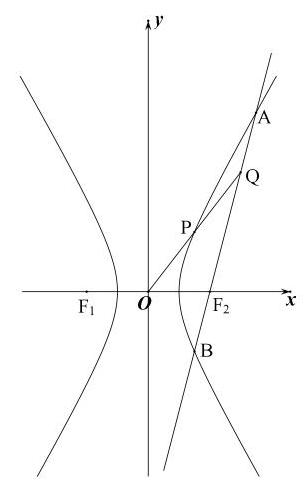
\includegraphics[max width=0.2\textwidth]{images/bo_d7fhnv491nqc73ercsbg_128_1105_993_305_489_0.jpg}
\end{center}
\hspace*{3em} 

由 \(\overrightarrow{AB} = 2\overrightarrow{Q{F}_{2}}\) 得 \(\left( {{x}_{2} - {x}_{1},{y}_{2} - {y}_{1}}\right)  = 2\left( {2 - 2{x}_{0}, - 2{y}_{0}}\right)\) ,

从而 \({x}_{2} - {x}_{1} = 2\left( {2 - 2{x}_{0}}\right)\) ,即 \({\left( {x}_{1} - {x}_{2}\right) }^{2} = {16}{\left( {x}_{0} - 1\right) }^{2}\) ,

将韦达定理代入 \({\left( \frac{4{k}^{2}}{{k}^{2} - 3}\right) }^{2} - 4 \times  \frac{4{k}^{2} + 3}{{k}^{2} - 3} = {16}{\left( {x}_{0} - 1\right) }^{2}\) ,

化简得 \(9\left( {{k}^{2} + 1}\right)  = 4{\left( {x}_{0} - 1\right) }^{2}{\left( {k}^{2} - 3\right) }^{2}\) (※)

.13 分

因为 \(k = {k}_{Q{F}_{2}} = \frac{2{y}_{0}}{2{x}_{0} - 2} = \frac{{y}_{0}}{{x}_{0} - 1}\) ,即 \({y}_{0} = k\left( {{x}_{0} - 1}\right)\) ,

由已知 \(P\left( {{x}_{0},{y}_{0}}\right)\) 在双曲线上,得 \(3{x}_{0}{}^{2} - {y}_{0}{}^{2} = 3\) ,

从而 \(3{x}_{0}{}^{2} - {\left( k\left( {x}_{0} - 1\right) \right) }^{2} = 3\) 得 \({k}^{2} = \frac{3{x}_{0}{}^{2} - 3}{{\left( {x}_{0} - 1\right) }^{2}} = \frac{3\left( {{x}_{0} + 1}\right) }{{x}_{0} - 1}\) 代入 (※) 式,

\(9\left( {\frac{3{x}_{0} + 3}{{x}_{0} - 1} + 1}\right)  = 4{\left( {x}_{0} - 1\right) }^{2}{\left( \frac{3{x}_{0} + 3}{{x}_{0} - 1} - 3\right) }^{2},\)

化简得 \(9\frac{4{x}_{0} + 2}{{x}_{0} - 1} = 4{\left( {x}_{0} - 1\right) }^{2}{\left( \frac{6}{{x}_{0} - 1}\right) }^{2}\) ,即 \(9\frac{4{x}_{0} + 2}{{x}_{0} - 1} = 4 \times  {36}\) ,

解得 \({x}_{0} = \frac{3}{2}\) .15 分点 \(P\) 的坐标为 \(\left( {\frac{3}{2},\frac{\sqrt{15}}{2}}\right)\) .16 分

8.(2025 高三二模闵行 20)已知双曲线 \(\Gamma  : {x}^{2} - \frac{{y}^{2}}{3} = 1\) 的右焦点为 \(F\) ，过点 \(F\) 的直线 \(l\) 交双曲线 \(\Gamma\) 右支于 \(A\) 、 \(B\) 两点(点 \(A\) 在 \(x\) 轴上方),点 \(C\) 在双曲线 \(\Gamma\) 上,直线 \({AC}\) 交 \(x\) 轴于点 \(Q\) (点 \(Q\) 在点 \(F\) 的右侧).

(1)求双曲线 \(\Gamma\) 的渐近线方程；

(2)若点 \(A\left( {2,3}\right)\) ，且 \(\tan \angle {BAC} = \frac{1}{2}\) ，求点 \(C\) 的坐标；

(3)若 \(\bigtriangleup  {ABC}\) 的重心 \(G\) 在 \(x\) 轴上，记 \(\bigtriangleup  {AFG}\) 、 \(\bigtriangleup  {CQG}\) 的面积分别为 \({S}_{1}\) 、 \({S}_{2}\) ，求 \(\frac{{S}_{1}}{{S}_{2}}\) 的最小值.

【答案】( 1 ) \(y =  \pm  \sqrt{3}x\) ；( 2 ) \(\left( {{26}, - {45}}\right)\) ；( 3 ) \(\frac{\sqrt{3}}{2} + 1\)

【解析】(1) 双曲线 \(\Gamma  : {x}^{2} - \frac{{y}^{2}}{3} = 1\) 的渐近线方程为: \(y =  \pm  \sqrt{3}x\) ; 4 分

(2)由题意知 \(F\left( {2,0}\right)\) ， \(A\left( {2,3}\right)\) ，设 \(C\left( {{x}_{0},{y}_{0}}\right)\) ，则由 \(\tan \angle {BAC} = \frac{1}{2}\) 得

\({k}_{AC} = \tan \left( {\angle {BAC} + {90}^{ \circ  }}\right)  =  - 2,\) .6 分

即 \(\frac{{y}_{0} - 3}{{x}_{0} - 2} =  - 2\) ,又由 \({x}_{0}{}^{2} - \frac{{y}_{0}{}^{2}}{3} = 1\) ,解得 \(\left\{  \begin{array}{l} {x}_{0} = {26}, \\  {y}_{0} =  - {45}, \end{array}\right.\)

所以点 \(C\) 的坐标为 \(\left( {{26}, - {45}}\right)\)

(3)法一:

\begin{center}
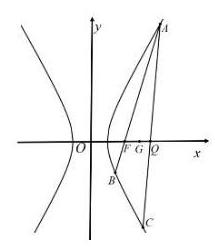
\includegraphics[max width=0.2\textwidth]{images/bo_d7fhnv491nqc73ercsbg_129_1284_1484_215_247_0.jpg}
\end{center}
\hspace*{3em} 

设直线 \(l : x = {my} + 2\) ,点 \(A\left( {{x}_{1},{y}_{1}}\right) \text{ 、 }B\left( {{x}_{2},{y}_{2}}\right) \text{ 、 }C\left( {{x}_{3},{y}_{3}}\right)\) ,

将直线 \(l\) 的方程代入双曲线方程后整理可得: \(\left( {3{m}^{2} - 1}\right) {y}^{2} + {12my} + 9 = 0\) ,

即有 \(\left\{  \begin{array}{l} \Delta  = {36}\left( {{m}^{2} + 1}\right)  > 0, \\  {y}_{1} + {y}_{2} = \frac{-{12m}}{3{m}^{2} - 1}, \\  {y}_{1}{y}_{2} = \frac{9}{3{m}^{2} - 1}. \end{array}\right.\) 12 分

因为直线 \(l\) 过点 \(F\) 且与双曲线 \(\Gamma\) 右支交于 \(A\text{ 、 }B\) 两点, \(\therefore m \in  \left( {-\frac{\sqrt{3}}{3},\frac{\sqrt{3}}{3}}\right)\) ,

又因为 \(\bigtriangleup  {ABC}\) 的重心 \(G\) 在 \(x\) 轴上，所以 \({y}_{1} + {y}_{2} + {y}_{3} = 0\) ，

由点 \(Q\) 在点 \(F\) 的右侧,可得 \({y}_{3} < 0\) ,所以 \({y}_{1} + {y}_{2} > 0\) ,

解得 \(m > 0\) ,所以 \(m \in  \left( {0,\frac{\sqrt{3}}{3}}\right)\) , 14 分

而 \(\left| {{y}_{1} - {y}_{2}}\right|  = \sqrt{{\left( {y}_{1} + {y}_{2}\right) }^{2} - 4{y}_{1}{y}_{2}}\) ,代入可得 \({y}_{1} - {y}_{2} =  - \frac{6\sqrt{{m}^{2} + 1}}{3{m}^{2} - 1}\) .

\(\frac{{S}_{1}}{{S}_{2}} = \frac{\frac{{S}_{1}}{{S}_{\bigtriangleup {ABG}}}}{\frac{{S}_{2}}{{S}_{\bigtriangleup {ACG}}}} = \frac{\frac{\left| AB\right| }{\left| AB\right| }}{\frac{\left| CQ\right| }{\left| AC\right| }} = \frac{\frac{{y}_{1}}{{y}_{1} - {y}_{2}}}{\frac{-{y}_{3}}{{y}_{1} - {y}_{3}}} = \frac{\frac{{y}_{1}}{{y}_{1} - {y}_{2}}}{\frac{{y}_{1} + {y}_{2}}{2{y}_{1} + {y}_{2}}} = \frac{\left( {{y}_{1} + {y}_{2} + {y}_{1}}\right) \left( {{y}_{1} + {y}_{2} - {y}_{2}}\right) }{\left( {{y}_{1} - {y}_{2}}\right) \left( {{y}_{1} + {y}_{2}}\right) }\)

\(= \frac{{y}_{1} + {y}_{2}}{{y}_{1} - {y}_{2}} + 1 - \frac{{y}_{1}{y}_{2}}{\left( {{y}_{1} + {y}_{2}}\right) \left( {{y}_{1} - {y}_{2}}\right) }\) ,代入后化简可得: \(\frac{{S}_{1}}{{S}_{2}} = \frac{{13}{m}^{2} + 1}{{8m}\sqrt{{m}^{2} + 1}} + 1\) .16 分

所以 \(\frac{{S}_{1}}{{S}_{2}} = \frac{{13}{m}^{2} + 1}{{8m}\sqrt{{m}^{2} + 1}} + 1 = \frac{{12}{m}^{2}}{{8m}\sqrt{{m}^{2} + 1}} + \frac{{m}^{2} + 1}{{8m}\sqrt{{m}^{2} + 1}} + 1 \geq  \frac{\sqrt{3}}{2} + 1\) ,

当且仅当 \(m = \frac{\sqrt{11}}{11}\) 时等号成立, \(\therefore \frac{{S}_{1}}{{S}_{2}}\) 的最小值为 \(\frac{\sqrt{3}}{2} + 1\ldots \ldots {18}\) 分

法二: 记 \(\overrightarrow{AF} = \lambda \overrightarrow{AB},\overrightarrow{AQ} = \mu \overrightarrow{AC}\) ,由重心 \(G\) 得 \(\overrightarrow{AG} = \frac{1}{3}\overrightarrow{AB} + \frac{1}{3}\overrightarrow{AC}\) ,

因为 \(\overrightarrow{AF} = \lambda \overrightarrow{AB},\overrightarrow{AQ} = \mu \overrightarrow{AC}\) ,得 \(\overrightarrow{AG} = \frac{1}{3\lambda }\overrightarrow{AF} + \frac{1}{3\mu }\overrightarrow{AQ}\) ,

所以 \(\frac{1}{\lambda } + \frac{1}{\mu } = 3\) ,而 \(\frac{{S}_{1}}{{S}_{2}} = \frac{\frac{{S}_{1}}{{S}_{\bigtriangleup {ABG}}}}{\frac{{S}_{2}}{{S}_{\bigtriangleup {ACG}}}} = \frac{\frac{\left| AF\right| }{\left| AB\right| }}{\frac{\left| CQ\right| }{\left| AC\right| }} = \frac{\lambda }{1 - \mu } = \frac{1}{4 - \left( {\frac{1}{\mu } + {3\mu }}\right) } \geq  \frac{1}{4 - 2\sqrt{3}} = \frac{\sqrt{3}}{2} + 1\) ,

“=”成立当且仅当 \(\left\{  \begin{array}{l} \lambda  = \frac{1}{3 - \sqrt{3}}, \\  \mu  = \frac{\sqrt{3}}{3}. \end{array}\right.\)

9.(2025 高三二模奉贤 20)如图 20-1，曲线 \(\Gamma\) 是 \(\frac{{x}^{2}}{4} + \frac{{y}^{2}}{{b}^{2}} = 1\left( {y \geq  0}\right)\) 与 \(\frac{{y}^{2}}{{b}^{2}} - \frac{{x}^{2}}{4} = 1\left( {y \geq  0}\right)\) 组合的.

\begin{center}
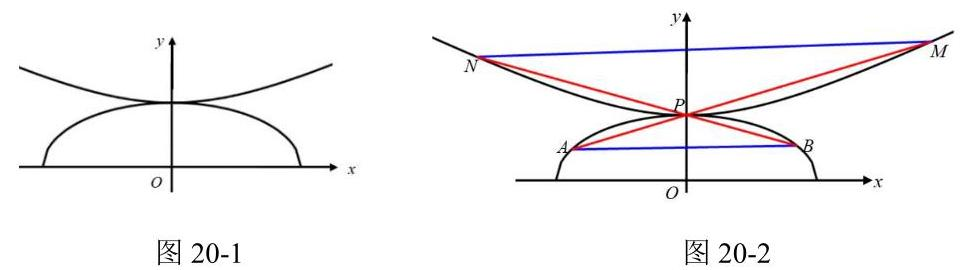
\includegraphics[max width=0.8\textwidth]{images/bo_d7fhnv491nqc73ercsbg_130_241_1813_965_270_0.jpg}
\end{center}
\hspace*{3em} 

第 20 题图

第 30 页(共 38 页)

(1) \(\frac{{x}^{2}}{4} + \frac{{y}^{2}}{{b}^{2}} = 1\left( {y \geq  0}\right)\) 过点 \(\left( {-1,\frac{3}{2}}\right)\) ，求 \(\frac{{y}^{2}}{{b}^{2}} - \frac{{x}^{2}}{4} = 1\left( {y \geq  0}\right)\) 的渐近线方程；

(2) \(b = \sqrt{2}\) ，设 \(T\left( {0,t}\right)\) ， \(t \in  \left\lbrack  {-\frac{\sqrt{2}}{2},3\sqrt{2}}\right\rbrack\) ，曲线 \(\Gamma\) 上找一个点 \(Q\) ，使得 \(\left| \overrightarrow{TQ}\right|\) 达到最小；

(3)若 \(b = 1\) ，如图 20-2，存在过点 \(P\left( {0,1}\right)\) 的两条直线 \({l}_{1},{l}_{2}\) 与曲线 \(\Gamma\) 的交点分别是点 \(A\) 、 点 \(M\) 、点 \(B\) 、点 \(N\) ,点 \(A\) 在第二象限,点 \(M\) 在第一象限.是否存在非零实数 \(\lambda\) 使得 \(\overrightarrow{MN} = \lambda \overrightarrow{AB}\) 成立,请说明理由.

【答案】(1) \(y =  \pm  \frac{\sqrt{3}}{2}x\) ; (2) 见解析; (3) 当 \({k}_{1} + {k}_{2} = 0\) 时,存在; 当 \({k}_{1} + {k}_{2} \neq  0\) 时,不存在.

【解析】(1) \(\left( {-1,\frac{3}{2}}\right)\) 代入 \(\frac{{x}^{2}}{4} + \frac{{y}^{2}}{{b}^{2}} = 1\) ,得 \({b}^{2} = 3\) 2 分

所以 \(\frac{{y}^{2}}{3} - \frac{{x}^{2}}{4} = 1\left( {y \geq  0}\right)\) ,渐近线方程: \(y =  \pm  \frac{\sqrt{3}}{2}x\) . 2 分

(2) \(b = \sqrt{2}\) ，曲线 \(\Gamma\) 是 \(\frac{{x}^{2}}{4} + \frac{{y}^{2}}{2} = 1\left( {y \geq  0}\right)\) 和 \(\frac{{y}^{2}}{2} - \frac{{x}^{2}}{4} = 1\left( {y \geq  0}\right)\) 的组合， 当 \(t \in  \left\lbrack  {-\frac{\sqrt{2}}{2},\sqrt{2}}\right\rbrack\) 时, \(\left| \overline{QT}\right|\) 取到最小值点 \(Q\) 一定在 \(\frac{{x}^{2}}{4} + \frac{{y}^{2}}{2} = 1\) 上, \(\therefore {x}^{2} = 4\left( {1 - \frac{{y}^{2}}{2}}\right) \left( {0 \leq  y \leq  \sqrt{2}}\right)\) ,

设点 \(Q\left( {x,y}\right)\) ，则 \(\left| \overrightarrow{TQ}\right|  = \sqrt{{x}^{2} + {\left( y - t\right) }^{2}}\) 1 分

\(\left| {TQ}\right|  = \sqrt{4 - 2{y}^{2} + {y}^{2} - {2ty} + {t}^{2}} = \sqrt{-{\left( y + t\right) }^{2} + 4 + 2{t}^{2}}\left( {0 \leq  y \leq  \sqrt{2}}\right)\) 1 分

当 \(t =  - \frac{\sqrt{2}}{2}\) 时,存在三个点 \(Q\left( {\pm 2,0}\right)\) 或 \(Q\left( {0,\sqrt{2}}\right) ,\left| \overline{QT}\right|\) 最小值 \(\frac{3\sqrt{2}}{2}\) , 1 分

当 \(- \frac{\sqrt{2}}{2} < t \leq  \sqrt{2}\) 时,存在唯一的点 \(Q\left( {0,\sqrt{2}}\right) ,\left| \overrightarrow{QT}\right|\) 最小值 \(\sqrt{2} - t\) , 1 分

当 \(t \in  \left( {\sqrt{2},3\sqrt{2}}\right\rbrack\) 时, \(\left| \overrightarrow{QT}\right|\) 取到最小值点 \(Q\) 一定在 \(\frac{{y}^{2}}{2} - \frac{{x}^{2}}{4} = 1\) 上,

\(\therefore {x}^{2} = 4\left( {\frac{{y}^{2}}{2} - 1}\right) \left( {y \geq  \sqrt{2}}\right)\) ,

\(\left| {TQ}\right|  = \sqrt{2{y}^{2} - 4 + {y}^{2} - {2ty} + {t}^{2}} = \sqrt{3{\left( y - \frac{t}{3}\right) }^{2} + 4 + \frac{2}{3}{t}^{2}}\left( {y > \sqrt{2}}\right) ,\;1\) 分

\(\because \sqrt{2} < t \leq  3\sqrt{2},\therefore \frac{\sqrt{2}}{3} < \frac{t}{3} \leq  \sqrt{2}\) 时存在唯一的点 \(Q\left( {0,\sqrt{2}}\right) ,\left| \overrightarrow{QT}\right|\) 最小值 \(t - \sqrt{2}\) . 1 分

(3)设 \({l}_{1} : y = {k}_{1}x + 1,{l}_{2} : y = {k}_{2}x + 1\) ，

设 \(A\left( {{x}_{1},{y}_{1}}\right) ,B\left( {{x}_{2},{y}_{2}}\right) ,M\left( {{x}_{3},{y}_{3}}\right) ,N\left( {{x}_{4},{y}_{4}}\right)\) ,

\(\left\{  {\begin{array}{l} y = {k}_{1}x + 1 \\  \frac{{x}^{2}}{4} + {y}^{2} = 1 \end{array} \Rightarrow  {x}_{1} = \frac{-8{k}_{1}}{4{k}_{1}^{2} + 1}\left( {0 < {k}_{1} < \frac{1}{2}}\right) ,\therefore A\left( {\frac{-8{k}_{1}}{4{k}_{1}^{2} + 1},\frac{-4{k}_{1}^{2} + 1}{4{k}_{1}^{2} + 1}}\right) ,}\right.\) 1 分

\(\left\{  {\begin{array}{l} y = {k}_{2}x + 1 \\  \frac{{x}^{2}}{4} + {y}^{2} = 1 \end{array} \Rightarrow  {x}_{2} = \frac{-8{k}_{2}}{4{k}_{2}{}^{2} + 1}\left( {-\frac{1}{2} < {k}_{2} < 0}\right) ,\;\therefore B\left( {\frac{-8{k}_{2}}{4{k}_{2}{}^{2} + 1},\frac{-4{k}_{2}{}^{2} + 1}{4{k}_{2}{}^{2} + 1}}\right) ,}\right.\) 1 分

\(\left\{  {\begin{array}{l} y = {k}_{1}x + 1 \\  {y}^{2} - \frac{{x}^{2}}{4} = 1 \end{array} \Rightarrow  {x}_{3} = \frac{-8{k}_{1}}{4{k}_{1}^{2} - 1}\left( {0 < {k}_{1} < \frac{1}{2}}\right) ,\;\therefore M\left( {-\frac{8{k}_{1}}{4{k}_{1}^{2} - 1},\frac{-4{k}_{1}^{2} - 1}{4{k}_{1}^{2} - 1}}\right) ,\;1}\right.\) 分

\(\left\{  {\begin{array}{l} y = {k}_{2}x + 1 \\  {y}^{2} - \frac{{x}^{2}}{4} = 1 \end{array} \Rightarrow  {x}_{4} = \frac{-8{k}_{2}}{4{k}_{2}{}^{2} - 1}\left( {-\frac{1}{2} < {k}_{2} < 0}\right) ,\therefore N\left( {-\frac{8{k}_{2}}{4{k}_{2}{}^{2} - 1},\frac{-4{k}_{2}{}^{2} - 1}{4{k}_{2}{}^{2} - 1}}\right) ,\;1}\right.\) 分

计算出 \({k}_{AB} = \frac{{k}_{1} + {k}_{2}}{1 - 4{k}_{1}{k}_{2}},{k}_{MN} = \frac{{k}_{1} + {k}_{2}}{1 + 4{k}_{1}{k}_{2}}\) , 2 分

当 \({k}_{1} + {k}_{2} = 0\) 时,存在非零实数 \(\lambda\) 使得 \(\overrightarrow{MN} = \lambda \overrightarrow{AB}\) 成立, 1 分

当 \({k}_{1} + {k}_{2} \neq  0\) 时,不存在实数 \(\lambda\) 使得 \(\overrightarrow{MN} = \lambda \overrightarrow{AB}\) 成立. 1 分

\section*{五、抛物线的综合}

1. (2025 高三二模松江 2)抛物线 \(C : {y}^{2} = {8x}\) 的焦点到准线的距离\_\_\_\_\_.

【答案】 4

【解析】焦点到准线的距离为 \(p,{2p} = 8\) ,解得 \(p = 4\) .

2.(2025 高三二模宝山 3)抛物线 \({x}^{2} = {4y}\) 的准线方程为\_\_\_\_\_.

【答案】 \(y =  - 1\)

【解析】 \(y =  - \frac{p}{2} =  - 1\) .

3.(2025 高三二模黄浦 3)抛物线 \({y}^{2} = x\) 的焦点到其顶点的距离为\_\_\_\_\_.

【答案】 \(\frac{1}{4}\)

【解析】焦点的坐标为 \(\left( {\frac{1}{4},0}\right)\) ,所以焦点到顶点的距离为 \(\frac{1}{4}\) .

4.(2025 高三二模普陀 5)设 \(m > 2\) ，抛物线 \(C : {x}^{2} = {2my}\) 上的点 \(P\) 到 \(C\) 的焦点的距离为 5， 点 \(P\) 到 \(y\) 轴的距离为 3,则 \(m\) 的值为\_\_\_\_\_.

【答案】 9

【解析】设 \(P\left( {x,y}\right)\) ,抛物线的准线方程为 \(y =  - \frac{m}{2}\) ,由题意可得 \(y + \frac{m}{2} = 5,x = 3\) ,

则有 \({3}^{2} = {2my} \Rightarrow  y = \frac{9}{2m}\) ,所以 \(\frac{9}{2m} + \frac{m}{2} = 5 \Rightarrow  m = 9\) 或 \(m = 1\) (舍),所以 \(m = 9\) .

5.(2025 高三二模浦东 8)设 \(M\left( {x,y}\right)\) 为抛物线 \({y}^{2} = {4x}\) 上任意一点，若 \(x + {2y} + m\) 的最小值为 1 , 则 \(m\) 的值为\_\_\_\_\_.

【答案】 5

【解析】因为 \(M\left( {x,y}\right)\) 为抛物线 \({y}^{2} = {4x}\) 上任意一点,所以 \(x = \frac{{y}^{2}}{4}\) ,

所以 \(x + {2y} + m = \frac{{y}^{2}}{4} + {2y} + m\) ,令 \(z = \frac{{y}^{2}}{4} + {2y} + m\) ,则二次函数的对称轴为 \(y =  - 4\) , 所以 \({z}_{\min } = \frac{{\left( -4\right) }^{2}}{4} + 2 \times  \left( {-4}\right)  + m = 1\) ,解得 \(m = 5\) .

6.(2025 高三二模青浦 10)已知点 \(P\) 是抛物线 \({y}^{2} = {8x}\) 上一动点，点 \(Q\) 在圆 \({\left( x - 5\right) }^{2} + {y}^{2} = 1\) 上运动，则 \(P\) 与 \(Q\) 两点间最短距离为\_\_\_\_\_.

【答案】 \(2\sqrt{6} - 1\)

【解析】设圆 \(Q\) 的圆心为 \(A\left( {5,0}\right)\) ,设 \(P\left( {x,y}\right)\) ,

\(\therefore {\left| PQ\right| }_{\min } = {\left( \left| PA\right|  - 1\right) }_{\min }\) ,

又 \(\left| {PA}\right|  = \sqrt{{\left( x - 5\right) }^{2} + {y}^{2}} = \sqrt{{\left( x - 5\right) }^{2} + {8x}} = \sqrt{{x}^{2} - {2x} + {25}} = \sqrt{{\left( x - 1\right) }^{2} + {24}}\) ,

\(\therefore {\left| PQ\right| }_{\min } = {\left( \left| PA\right|  - 1\right) }_{\min } = 2\sqrt{6} - 1\) .

7.(2025 高三二模徐汇 20)已知抛物线 \(C : {y}^{2} = {4x}\) ，点 \(F\) 是抛物线 \(C\) 的焦点.

(1)求点 \(F\) 的坐标及点 \(F\) 到准线 \(l\) 的距离；

\begin{center}
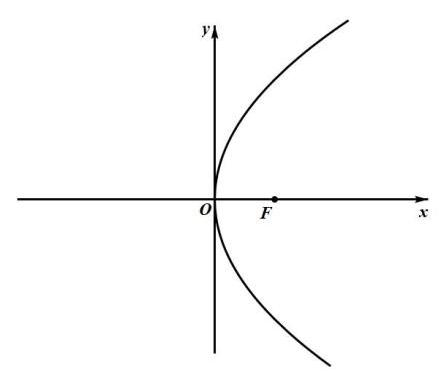
\includegraphics[max width=0.3\textwidth]{images/bo_d7fhnv491nqc73ercsbg_133_1152_1447_439_377_0.jpg}
\end{center}
\hspace*{3em} 

(2)过点 \(F\) 作相互垂直的两条直线 \({l}_{1},{l}_{2},{l}_{1}\) 交抛物线 \(C\) 于点 \({P}_{1}\) 、 \({P}_{2},{l}_{2}\) 交抛物线 \(C\) 于点 \({Q}_{1}\text{ 、 }{Q}_{2}\) ,求证: \(\frac{1}{\left| {P}_{1}{P}_{2}\right| } + \frac{1}{\left| {Q}_{1}{Q}_{2}\right| }\) 为定值, 并求出该定值;

(3)过点 \(F\) 且斜率为 \(\sqrt{3}\) 的直线交抛物线 \(C\) 于 \(A\) 、 \(B\) 两点，设点 \(P\) 不在直线 \({AB}\) 上且 \({PF}\) 为 \(\bigtriangleup {PAB}\) 的内角平分线,求 \(\bigtriangleup {PAB}\) 面积的最大值.

【答案】(1)2 ; (2) \(\frac{1}{\left| {P}_{1}{P}_{2}\right| } + \frac{1}{\left| {Q}_{1}{Q}_{2}\right| } = \frac{1}{4}\) ,证明见解析；(3) \(\frac{16}{3}\)

【解析】(1) 由已知可得 \({2p} = 4\) ,即 \(p = 2\) ,

所以点 \(F\) 的坐标为 \(\left( {1,0}\right)\) ,

点 \(F\) 到准线 \(l\) 的距离为 2 .

(2)证明:由已知可知直线 \({l}_{1},{l}_{2}\) 的斜率存在且不等于 0 并过点 \(F\left( {1,0}\right)\) ， 设 \({l}_{1}\) 的方程为 \(y = k\left( {x - 1}\right) \left( {k \neq  0}\right)\) ， \({l}_{1}\) 与 \(C\) 相交于 \({P}_{1}\left( {{x}_{1},{y}_{1}}\right) ,{P}_{2}\left( {{x}_{2},{y}_{2}}\right)\) ， 由 \(\left\{  \begin{array}{l} {y}^{2} = {4x} \\  y = k\left( {x - 1}\right)  \end{array}\right.\) 得 \({k}^{2}{x}^{2} - \left( {2{k}^{2} + 4}\right) x + {k}^{2} = 0\) ,

则 \({x}_{1} + {x}_{2} = \frac{2{k}^{2} + 4}{{k}^{2}},{x}_{1}{x}_{2} = 1\) ,

\(\left| {{P}_{1}{P}_{2}}\right|  = {x}_{1} + {x}_{2} + 2 = \frac{2{k}^{2} + 4}{{k}^{2}} + 2 = \frac{4{k}^{2} + 4}{{k}^{2}}\) ,

同理可得 \(\left| {{Q}_{1}{Q}_{2}}\right|  = \frac{4{\left( -\frac{1}{k}\right) }^{2} + 4}{{\left( -\frac{1}{k}\right) }^{2}} = 4{k}^{2} + 4\) ,

所以 \(\frac{1}{\left| {P}_{1}{P}_{2}\right| } + \frac{1}{\left| {Q}_{1}{Q}_{2}\right| } = \frac{{k}^{2}}{4{k}^{2} + 4} + \frac{1}{4{k}^{2} + 4} = \frac{1}{4}\) .

(3)由已知可得直线 \({AB}\) 的方程为 \(y = \sqrt{3}\left( {x - 1}\right)\) ，

由 \(\left\{  \begin{array}{l} y = \sqrt{3}\left( {x - 1}\right) \\  {y}^{2} = {4x} \end{array}\right.\) ,解得 \(\left\{  \begin{array}{l} {x}_{1} = \frac{1}{3} \\  {y}_{1} =  - \frac{2\sqrt{3}}{3} \end{array}\right.\) , \(\left\{  \begin{array}{l} {x}_{1} = 3 \\  {y}_{1} = 2\sqrt{3} \end{array}\right.\) ,不妨令 \(B\left( {\frac{1}{3}, - \frac{2\sqrt{3}}{3}}\right) ,A\left( {3,2\sqrt{3}}\right)\) ,

则 \(\left| {AB}\right|  = \frac{1}{3} + 1 + 3 + 1 = \frac{16}{3},\frac{\left| AF\right| }{\left| BF\right| } = \frac{3 + 1}{\frac{1}{3} + 1} = 3\) ,

在 \(\bigtriangleup {PAF}\) 中, \(\frac{\left| PA\right| }{\sin \angle {PFA}} = \frac{\left| AF\right| }{\sin \angle {APF}}\) ,

在 \(\bigtriangleup {PBF}\) 中, \(\frac{\left| PB\right| }{\sin \angle {PFB}} = \frac{\left| BF\right| }{\sin \angle {BPF}}\) ,

由 \(\angle {PFA} + \angle {PFB} = \pi\) 及 \(\angle {APF} = \angle {BPF}\) 得 \(\frac{\left| PA\right| }{\left| PB\right| } = \frac{\left| AF\right| }{\left| BF\right| } = 3\)

设点 \(P\left( {x,y}\right)\) ,于是 \(\sqrt{{\left( x - 3\right) }^{2} + {\left( y - 2\sqrt{3}\right) }^{2}} = 3\sqrt{{\left( x - \frac{1}{3}\right) }^{2} + {\left( y + \frac{2\sqrt{3}}{3}\right) }^{2}}\) ,

整理得 \({x}^{2} + {\left( y + \sqrt{3}\right) }^{2} = 4\) ,

所以点 \(P\) 在以点 \(\left( {0, - \sqrt{3}}\right)\) 为圆心,2 为半径的圆上 (除去与直线 \({AB}\) 的两个交点),

因为圆心 \(\left( {0, - \sqrt{3}}\right)\) 在直线 \({AB}\) 上,则点 \(P\) 到直线 \({AB}\) 距离的最大值为 2,

所以 \(\bigtriangleup {PAB}\) 面积最大值为 \(\frac{1}{2} \times  2 \times  \frac{16}{3} = \frac{16}{3}\) .

8.(2025 高三二模静安 20)如图，在直角坐标平面 \({xOy}\) 中， \(\bigtriangleup {A}_{i}{B}_{i}{A}_{i + 1}\) 中( \(i = 1,2,\cdots ,n,\cdots\) ) 为正三角形,且满足 \(\overrightarrow{O{A}_{1}} = \left( {-\frac{1}{4},0}\right) ,\overrightarrow{{A}_{i}{A}_{i + 1}} = \left( {{2i} - 1,0}\right)\) .

(1)求点 \({A}_{n}\) 的横坐标 \({X}_{n}\) 关于正整数 \(n\) 的表达式；

(2)求证:点 \({B}_{1},{B}_{2},\cdots ,{B}_{n}\cdots\) 在抛物线 \(\Gamma  : {y}^{2} = {3x}\) 上；

(3)过(2)中抛物线 \(\Gamma  : {y}^{2} = {3x}\) 的焦点 \(F\) 作两条互相垂直的弦 \({AC}\) 和 \({BD}\) ，求四边形 \({ABCD}\) 面积的最小值.

\begin{center}
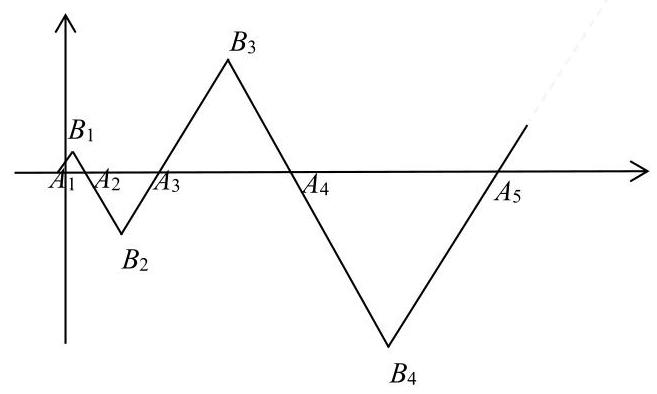
\includegraphics[max width=0.5\textwidth]{images/bo_d7fhnv491nqc73ercsbg_135_341_1149_657_394_0.jpg}
\end{center}
\hspace*{3em} 

【答案】( 1 ) \({X}_{n} =  - \frac{1}{4} + {\left( n - 1\right) }^{2}\) ；( 2 )证明见解析；( 3 )\_\_\_\_\_

\begin{center}
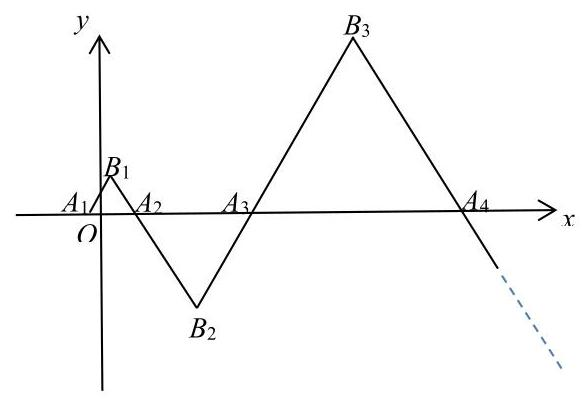
\includegraphics[max width=0.4\textwidth]{images/bo_d7fhnv491nqc73ercsbg_135_972_1667_582_399_0.jpg}
\end{center}
\hspace*{3em} 

【解析】(1) \(\overrightarrow{O{A}_{n}} = \overrightarrow{O{A}_{1}} + \overrightarrow{{A}_{1}{A}_{2}} + \cdots  + \overrightarrow{{A}_{n - 1}{A}_{n}}\) ， \({X}_{n} =  - \frac{1}{4} + \mathop{\sum }\limits_{{i = 1}}^{{n - 1}}\left( {{2i} - 1}\right)  =  - \frac{1}{4} + {\left( n - 1\right) }^{2}\) . (4 分)

(2)点 \({B}_{n}\) 的坐标为 \(\left( {x,y}\right)\) ，则

\(\left\{  {\begin{array}{l} x =  - \frac{1}{4} + {\left( n - 1\right) }^{2} + \frac{{2n} - 1}{2}, \\  \left| y\right|  = \frac{\sqrt{3}}{2}\left( {{2n} - 1}\right) . \end{array}\text{ 即 }\left\{  \begin{array}{l} x = {\left( n - \frac{1}{2}\right) }^{2}, \\  \left| y\right|  = \frac{\sqrt{3}}{2}\left( {{2n} - 1}\right) . \end{array}\right. }\right.\)

满足方程 \({y}^{2} = {3x}\) ,故点 \({B}_{1},{B}_{2},\cdots ,{B}_{n}\cdots\) 在抛物线 \(\Gamma  : {y}^{2} = {3x}\) 上. (6 分)

(3)抛物线 \(\Gamma  : {y}^{2} = {3x}\) 的焦点为 \(F\left( {\frac{3}{4},0}\right)\) . (1 分)

互相垂直的弦 \({AC}\) 和 \({BD}\) 显然都不垂直坐标轴,设直线 \({AC}\) 的方程为 \(x = {my} + \frac{3}{4}\) ,

分)

代入 \(\Gamma  : {y}^{2} = {3x}\) ,得 \({y}^{2} - {3my} - \frac{9}{4} = 0\) . 所以有 \({y}_{A} + {y}_{C} = {3m},{y}_{A} + {y}_{C} =  - \frac{9}{4}\) ,

所以, \(\left| {AC}\right|  = \sqrt{1 + {m}^{2}}\left| {{y}_{A} - {y}_{C}}\right|  = 3\left( {1 + {m}^{2}}\right)\) . (1 分)

将上式中的 \(m\) 用 \(- \frac{1}{m}\) 代换,得 \(\left| {BD}\right|  = 3\left( {1 + \frac{1}{{m}^{2}}}\right)\) ,(1 分)

于是 \({S}_{ABCD} = \frac{1}{2}\left| {AC}\right|  \cdot  \left| {BD}\right|  = \frac{9}{2}\left( {1 + {m}^{2}}\right) \left( {1 + \frac{1}{{m}^{2}}}\right)  = \frac{9}{2}\left( {2 + {m}^{2} + \frac{1}{{m}^{2}}}\right)  \geq  {18}\) .

当且仅当 \(m =  \pm  1\) 时,上式等号成立. 故四边形 \({ABCD}\) 面积的最小值为 18. (4 分)

\begin{center}
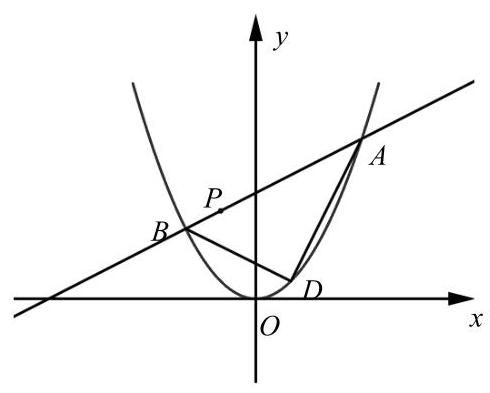
\includegraphics[max width=0.4\textwidth]{images/bo_d7fhnv491nqc73ercsbg_136_1118_1355_490_393_0.jpg}
\end{center}
\hspace*{3em} 

第(3)小题图

9.(2025 高三二模崇明 20)已知抛物线 \(\Gamma  : {x}^{2} = {4y}\) ，过点 \(P\left( {a,b}\right)\) 的直线 \(l\) 与抛物线 \(\Gamma\) 交于点 \(A\text{ 、 }B\) ,与 \(y\) 轴交于点 \(C\) .

(1)若点 \(A\) 位于第一象限，且点 \(A\) 到抛物线 \(\Gamma\) 的焦点的距离等于 3， 求点 \(A\) 的坐标；

(2)若点 \(A\) 坐标为 \(\left( {4,4}\right)\) ，且点 \(B\) 恰为线段 \({AC}\) 的中点，求原点 \(O\) 到直线 \(l\) 的距离；

(3)若抛物线 \(\Gamma\) 上存在定点 \(D\) 使得满足题意的点 \(A\) 、 \(B\) 都有 \({DA} \bot  {DB}\) ,求 \(a\text{ 、 }b\) 满足的关系式.

【答案】(1) \(\left( {2\sqrt{2},2}\right)\) ; (2) \(\frac{4\sqrt{13}}{13}\) ; (3) \({a}^{2} = {4b} - {16}\)

【解析】(1) 设 \(A\left( {x,y}\right) \left( {x,y > 0}\right)\) ,因为点 \(A\) 在抛物线上,所以点 \(A\) 到抛物线 \(\Gamma\) 的焦点的距离等于它到抛物线 \(\Gamma\) 的准线 \(y =  - 1\) 的距离,所以 \(y + 1 = 3,y = 2\) ,所以 \(x = 4\sqrt{2}\) ,

故点 \(A\) 的坐标是 \(\left( {2\sqrt{2},2}\right)\) .4 分

(2)设 \(B\left( {b,\frac{{b}^{2}}{4}}\right)\) ，则 \(C\left( {{2b} - 4,\frac{{b}^{2}}{2} - 4}\right)\) ，由题意， \(4 - {2b} = 0\) ，所以 \(b = 2\) ， .2 分所以 \(B\) 点坐标为 \(\left( {2,1}\right)\) ,直线 \(l\) 的方程为: \({3x} - {2y} - 4 = 0\) .4 分所以原点 \(O\) 到直线 \(l\) 的距离 \(d = \frac{\left| -4\right| }{\sqrt{{3}^{2} + {\left( -2\right) }^{2}}} = \frac{4\sqrt{13}}{13}\) .6 分

(3)设 \(D\left( {{x}_{0},\frac{{x}_{0}^{2}}{4}}\right)\) ，由题意，直线 \(l\) 斜率必然存在，设其方程为: \(y - b = k\left( {x - a}\right)\) ，

代入 \({x}^{2} = {4y}\) 中，得: \({x}^{2} - {4kx} + {4ka} - {4b} = 0\) ，

设 \(A\left( {{x}_{1},\frac{{x}_{1}^{2}}{4}}\right) ,B\left( {{x}_{2},\frac{{x}_{2}^{2}}{4}}\right)\) ,则 \({x}_{1} + {x}_{2} = {4k},{x}_{1}{x}_{2} = {4ka} - {4b}\) .3 分

因为 \({DA} \bot  {DB}\) ,所以 \(\overrightarrow{DA} \cdot  \overrightarrow{DB} = \left( {{x}_{1} - {x}_{0},\frac{{x}_{1}^{2}}{4} - \frac{{x}_{0}^{2}}{4}}\right)  \cdot  \left( {{x}_{2} - {x}_{0},\frac{{x}_{2}^{2}}{4} - \frac{{x}_{0}^{2}}{4}}\right)  = 0\) ,

所以 \({x}_{1}{x}_{2} + \left( {{x}_{1} + {x}_{2}}\right) {x}_{0} + {x}_{0}^{2} + {16} = 0\) ,

故 \({4ka} - {4b} + {4k}{x}_{0} + {x}_{0}^{2} + {16} = 0\) ,即 \(4\left( {a + {x}_{0}}\right) k + {x}_{0}^{2} + {16} - {4b} = 0\) .6 分

由题意,得 \(\left\{  \begin{array}{l} {x}_{0} =  - a \\  {x}_{0}^{2} = {4b} - {16} \end{array}\right.\) ,因此 \({a}^{2} = {4b} - {16}\) ..8 分

\section*{六、解析几何新定义}

1.(2025 高三二模浦东 16)已知圆锥曲线 \(\Gamma\) 的对称中心为原点 \(O\) ，若对于 \(\Gamma\) 上的任意一点 \(A\) ， 均存在 \(\Gamma\) 上两点 \(B,C\) ，使得原点 \(O\) 到直线 \({AB},{AC}\) 和 \({BC}\) 的距离都相等，则称曲线 \(\Gamma\) 为“完美曲线”. 现有如下两个命题:

 \circled{1} 任意椭圆都是“完美曲线”； \circled{2} 存在双曲线是“完美曲线”.

下列判断正确的是( )

A.  \circled{1} 是真命题， \circled{2} 是假命题 B.  \circled{1} 是假命题， \circled{2} 是真命题

C.  \circled{1}  \circled{2} 都是真命题 D.  \circled{1}  \circled{2} 都是假命题

【答案】A

【解析】 \circled{1} 对于椭圆上任意一点 \(A\) ,以 \({AO}\) 为角平分线做两条射线 \({AB},{AC}\) 交椭圆于 \(B\) , \(C\) 两点,此时,原点 \(O\) 到直线 \({AB},{AC}\) 距离都相等,

当 \(\angle {OAB}\) 趋近于 0 时,点 \(O\) 到 \({AB},{AC}\) 距离的距离较小,到 \({BC}\) 的距离较大,当 \({BC}\) 经过点 \(O\) 时,点 \(O\) 到 \({AB},{AC}\) 距离较大,到 \({BC}\) 的距离为 0,

第 37页(共 38页)

所以在 \(\angle {OAB}\) 从 0 变大的过程中,必存在某一刻,使原点 \(O\) 到直线 \({AB},{AC}\) 和 \({BC}\) 的距离都相等, 所以 \circled{1} 正确；

 \circled{2} 以双曲线 \(\frac{{x}^{2}}{{a}^{2}} - \frac{{y}^{2}}{{b}^{2}} = 1\left( {a > 0,b > 0}\right)\) 为例，取 \(A\) 为左顶点 \(\left( {-a,0}\right)\) ，

因为原点 \(O\) 到 \({AB},{AC}\) 距离相等,所以 \(\angle {OAB} = \angle {OAC}\) ,所以 \(B,C\) 关于 \(x\) 轴对称,

所以点 \(O\) 到 \({BC}\) 的距离必大于 \(a\) ,而点 \(O\) 到经过点 \(A\) 的直线距离的最大值为 \(a\) ,

故 \(B,C\) 两点不存在,所以 \circled{2} 错误;

故选 A.

\section*{第七部分 立体几何}

\section*{一、线线、线面、面面位置关系}

1. (2025 高三二模嘉定 14)已知平面 \(\alpha\) 和平面 \(\beta\) ，直线 \(m \subset  \alpha\) ，直线 \(n \subset  \beta\) ，则下列结论一定成立的是( )

A. 若 \(m//n\) ，则 \(\alpha //\beta\)

C. 若 \(m \bot  n\) ，则 \(\alpha  \bot  \beta \;\) D. 若 \(n \bot  \alpha\) ，则 \(m \bot  n\)

【答案】D

【解析】A.若 \(m//n\) ,则平面 \(\alpha\) 和平面 \(\beta\) 可以平行,也可以相交,所以错误;

B. 若 \(m\) 与 \(n\) 为异面直线,则平面 \(\alpha\) 和平面 \(\beta\) 可以平行,也可以相交,所以错误;

C. 若 \(m \bot  n\) ,则平面 \(\alpha\) 和平面 \(\beta\) 可以平行,也可以相交,所以错误;

D. 若 \(n \bot  \alpha\) ,则 \(n\) 垂直平面 \(\alpha\) 内所有直线,又 \(m \subset  \alpha\) ,所以 \(m \bot  n\) ,正确,故选 D.

2. (2025 高三二模长宁 15) 如图，等腰直角三角形 \({ABC}\) 中， \(\angle A = {90}^{ \circ  }\) ，点 \(E\) 是边 \({AC}\) 的中点,点 \(D\) 是边 \({BC}\) 上一点 (不与 \(C\) 重合),将三角形 \({DCE}\) 沿 \({DE}\) 逆时针翻折,点 \(C\) 的对应点是 \({C}_{1}\) ,连接 \(C{C}_{1}\) ,设 \(\theta\) 为二面角 \({C}_{1} - {DE} - C\) 大小, \(\theta  \in  \left( {0,\pi }\right)\) . 在翻折过程中,下列说法当中不正确的是( )

\begin{center}
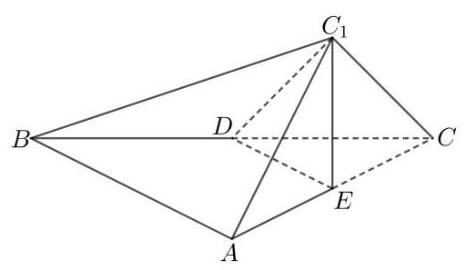
\includegraphics[max width=0.3\textwidth]{images/bo_d7fhnv491nqc73ercsbg_139_882_1259_464_270_0.jpg}
\end{center}
\hspace*{3em} 

A. 存在点 \(D\) 和 \(\theta\) ,使得 \(D{C}_{1} \bot  {AC}\)

B. 存在点 \(D\) 和 \(\theta\) ,使得 \(B{C}_{1} \bot  {AC}\)

C. 存在点 \(D\) 和 \(\theta\) ,使得 \(B{C}_{1} \bot  {DE}\)

D. 存在点 \(D\) 和 \(\theta\) ,使得 \(C{C}_{1} \bot  {DE}\)

【答案】B

【解析】对于 \(\mathrm{{AD}}\) ,取 \(D\) 为 \({BC}\) 中点, \(\theta  = \frac{\pi }{2}\) ,则 \({ED}//{AB}\) ,而 \({AB} \bot  {AC}\) ,

故 \({DE}\bot {AC}\) ,故在几何体 \({C}_{1} - {ABDE}\) 中， \({DE}\bot {C}_{1}E\) ,

而 \({CE} \bot  {DE}\) ,故 \(\angle {CE}{C}_{1}\) 为二面角 \({C}_{1} - {DE} - C\) 的平面角，故 \(\angle {CE}{C}_{1} = {90}^{ \circ  }\) ,

故 \({C}_{1}E \bot  {AC}\) ,而 \({C}_{1}E \cap  {DE} = E,{C}_{1}E,{DE} \subset\) 平面 \({DE}{C}_{1}\) ,

故 \({AC} \bot\) 平面 \({DE}{C}_{1}\) ,而 \(D{C}_{1} \subset\) 平面 \({DE}{C}_{1}\) ,故 \({AC} \bot  D{C}_{1}\) ,故 A 成立;

因 \({DE} \bot  {AC},{DE} \bot  {C}_{1}E,{AC} \cap  {C}_{1}E = E,{AC},{C}_{1}E \subset\) 平面 \({AC}{C}_{1}\) ,

故 \({DE}\bot\) 平面 \({AC}{C}_{1}\) ，而 \(C{C}_{1} \subset\) 平面 \({AC}{C}_{1}\) ，故 \({DE}\bot C{C}_{1}\) ，故 D 成立；

对于 \(\mathrm{C}\) ,过 \(E\) 作 \({DE} \bot  {BC}\) , \(D\) 为垂足，取 \(\theta  = \frac{\pi }{2}\) ，同理可证 \({DE} \bot\) 平面 \({BC}{C}_{1}\) ，

而 \(B{C}_{1} \subset\) 平面 \({BC}{C}_{1}\) ,故 \({DE} \bot  B{C}_{1}\) ,故 \(\mathrm{C}\) 成立; 对于 \(\mathrm{B}\) ,过 \({C}_{1}\) 作 \({C}_{1}H \bot\) 平面 \({ABC}\) ,垂足为 \(H\) , 因为 \({AC} \subset\) 平面 \({ABC}\) ,故 \({C}_{1}H \bot  {AC}\) ,

\begin{center}
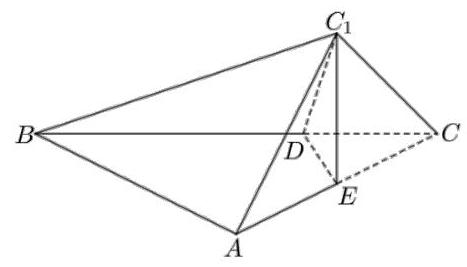
\includegraphics[max width=0.3\textwidth]{images/bo_d7fhnv491nqc73ercsbg_140_948_370_467_267_0.jpg}
\end{center}
\hspace*{3em} 

若 \(B{C}_{1} \bot  {AC}\) ,因为 \({C}_{1}H \cap  B{C}_{1} = {C}_{1}\)

\begin{center}
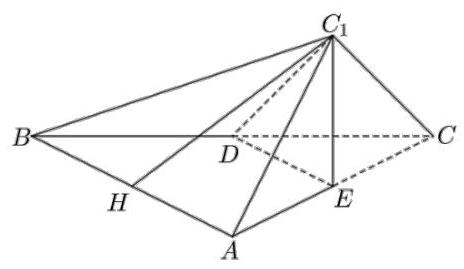
\includegraphics[max width=0.3\textwidth]{images/bo_d7fhnv491nqc73ercsbg_140_923_681_464_269_0.jpg}
\end{center}
\hspace*{3em} 

\({C}_{1}H,B{C}_{1} \subset\) 平面 \(B{C}_{1}H\) ,

故 \({AC} \bot\) 平面 \(B{C}_{1}H\) ，而 \({BH} \subset\) 平面 \(B{C}_{1}H\) ， 故 \({AC} \bot  {BH}\) ,

而 \({AC} \bot  {BA}\) ,故 \(H\) 在 \({BA}\) 上,

因为 \({C}_{1}H \cap  {BA} = H,{C}_{1}H,{BA} \subset\) 平面 \(B{C}_{1}A\) ,故 \({AC} \bot\) 平面 \(B{C}_{1}A\) ,

而 \({C}_{1}A \subset\) 平面 \(B{C}_{1}A\) ,故 \({CA} \bot  {C}_{1}A\) ,故 \({C}_{1}E > {AE}\) ,但 \({C}_{1}E = {CE} = {AE}\) ,

矛盾,故 \(B{C}_{1} \bot  {AC}\) 不成立即 \(\mathrm{B}\) 不成立.

\section*{二、异面直线所成角}

1. (2025 高三二模青浦 12)如图，正方体 \({ABCD} - {A}_{1}{B}_{1}{C}_{1}{D}_{1}\) 绕直线 \(D{B}_{1}\) 旋转 \(\frac{\pi }{3}\) ，直线 \({AB}\) 旋转至直线 \({A}^{\prime }{B}^{\prime }\) ，则直线 \({AB}\) 与直线 \({A}^{\prime }{B}^{\prime }\) 所成角的大小为\_\_\_\_\_.

【答案】 \(\arccos \frac{2}{3}\)

\begin{center}
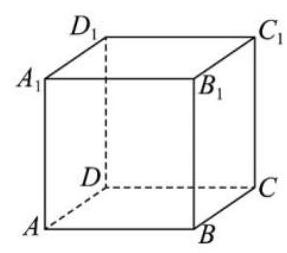
\includegraphics[max width=0.2\textwidth]{images/bo_d7fhnv491nqc73ercsbg_140_1211_1435_287_253_0.jpg}
\end{center}
\hspace*{3em} 

\begin{center}
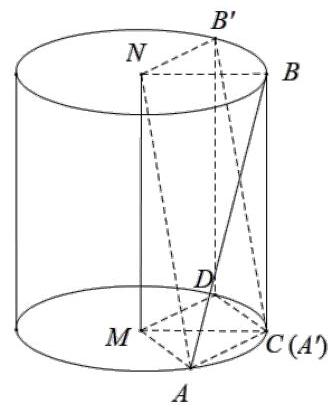
\includegraphics[max width=0.2\textwidth]{images/bo_d7fhnv491nqc73ercsbg_140_1200_1754_334_410_0.jpg}
\end{center}
\hspace*{3em} 

【解析】过点 \(A\) 作 \({AM} \bot  D{B}_{1}\) 于点 \(M\) ,过点 \(B\) 作 \({BN} \bot  D{B}_{1}\) 于点 \(N\) , 根据等面积法易算出 \({AM} = {BN} = \frac{\sqrt{6}}{3},{MN} = \frac{\sqrt{3}}{3}\) ，以 \({MN}\) 为轴构造圆柱如图所示,设点 \(B\) 在底面圆 \(M\) 上的射影为 \(C\) ,易知直线 \({AB}\) 与直线 \(D{B}_{1}\) 所成角的大小为 \(\arccos \frac{\sqrt{3}}{3}\) ,所以 \(\cos \angle {ABC} = \frac{\sqrt{3}}{3}\) ,

又由于 \({BC} = {MN} = \frac{\sqrt{3}}{3}\) ，所以 \({AC} = \frac{\sqrt{6}}{3}\) ，所以 \({\Delta AMC}\) 为等边三角形，

所以点 \(C\) 即为点 \({A}^{\prime }\) . 设点 \({B}^{\prime }\) 在底面圆 \(M\) 上的射影为 \(D\) ,则 \(\angle {DM}{A}^{\prime } = \angle {B}^{\prime }{NB} = \frac{\pi }{3}\) ,所以四边形 \({AMDC}\) 是菱形,所以 \({MD}\underline{\underline{I}}/{AC}\) ,又因为 \({MD}\underline{\underline{I}}//N{B}^{\prime }\) ,所以 \(A{A}^{\prime }\underline{\underline{I}}//N{B}^{\prime }\) ,所以四边形 \(A{A}^{\prime }{B}^{\prime }N\) 是平行四边形,所以 \({A}^{\prime }{B}^{\prime }//{AN}\) ,所以 \(\angle {BAN}\) 是所求角,

\(\cos \angle {BAN} = \frac{{1}^{2} + {1}^{2} - {\left( \frac{\sqrt{6}}{3}\right) }^{2}}{2 \times  1 \times  1} = \frac{2}{3}\) ，所以直线 \({AB}\) 与直线 \({A}^{\prime }{B}^{\prime }\) 所成角的大小为 \(\arccos \frac{2}{3}\) .

\section*{三、直线与平面所成角}

\begin{center}
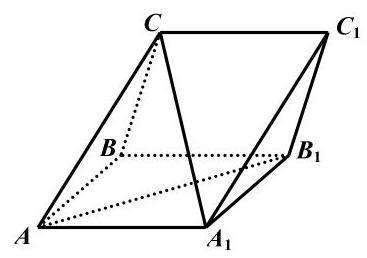
\includegraphics[max width=0.3\textwidth]{images/bo_d7fhnv491nqc73ercsbg_141_1060_773_367_258_0.jpg}
\end{center}
\hspace*{3em} 

1. (2025 高三二模普陀 17)如图，在三棱柱 \({ABC} - {A}_{1}{B}_{1}{C}_{1}\) 中， \({AC} = {A{A}_{1}} = {AB} = 2\) ， \(\angle {BA}{A}_{1} = \frac{\pi }{3}\) ,且 \(C{A}_{1} = {CB},C{A}_{1} \bot  A{B}_{1}\) .

(1)求证:平面 \({CA}{B}_{1} \bot\) 平面 \(A{A}_{1}{B}_{1}B\) ；

(2)求直线 \(C{A}_{1}\) 与平面 \(B{B}_{1}{C}_{1}C\) 所成的角的正弦值.

【答案】(1)证明见解析; (2) \(\frac{\sqrt{42}}{7}\)

\begin{center}
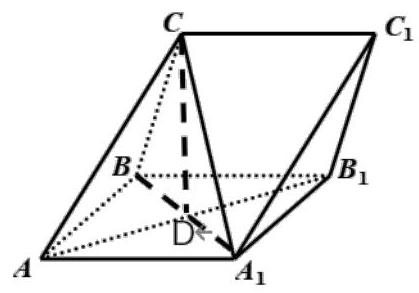
\includegraphics[max width=0.3\textwidth]{images/bo_d7fhnv491nqc73ercsbg_141_1028_1204_419_293_0.jpg}
\end{center}
\hspace*{3em} 

【解析】(1) 连接 \({A}_{1}B,{A}_{1}B\) 与 \(A{B}_{1}\) 交于 \(D\) 点,连接 \({CD}\) , 由条件得,四边形 \(A{A}_{1}{B}_{1}B\) 是菱形,则 \(A{B}_{1} \bot  {A}_{1}B\) ,

又 \(C{A}_{1} \bot  A{B}_{1},{A}_{1}B \cap  {A}_{1}C = {A}_{1}\) ,则 \(A{B}_{1} \bot\) 平面 \(C{A}_{1}B\) ,

又 \({CD} \subset\) 平面 \(C{A}_{1}B\) ,则 \(A{B}_{1} \bot  {CD}\) , .4 分

又 \({CB} = {CA}\) ，且 \(D\) 是 \({A}_{1}B\) 中点，则 \({A}_{1}B \bot  {CD}\) ，

则 \({CD} \bot\) 平面 \(A{A}_{1}{B}_{1}B\) ,

又 \({CD} \subset\) 平面 \({CA}{B}_{1}\) ,则平面 \({CA}{B}_{1} \bot\) 平面 \(A{A}_{1}{B}_{1}B\) . .6 分

(2)以 \(D\) 为原点， \(\overrightarrow{D{B}_{1}},\overrightarrow{DB},\overrightarrow{DC}\) 分别为 \(x,y,z\) 轴正方向建立空间直角坐标系， 则 \({B}_{1}\left( {\sqrt{3},0,0}\right) ,B\left( {0,1,0}\right) ,C\left( {0,0,1}\right) ,{A}_{1}\left( {0, - 1,0}\right) ,\overrightarrow{C{A}_{1}} = \left( {0,1,1}\right)\) , .4 分设平面 \(B{B}_{1}{C}_{1}C\) 的法向量为 \(\overrightarrow{n}\) ,由 \(\left\{  \begin{array}{l} \overrightarrow{n} \cdot  \overrightarrow{B{B}_{1}} = 0 \\  \overrightarrow{n} \cdot  \overrightarrow{BC} = 0 \end{array}\right.\) ,解得 \(\overrightarrow{n} = \left( {1,\sqrt{3},\sqrt{3}}\right)\) , .6 分

设直线 \(C{A}_{1}\) 与平面 \(B{B}_{1}{C}_{1}C\) 所成的角为 \(\theta\) ,则 \(\sin \theta  = \left| \frac{\overrightarrow{n} \cdot  \overrightarrow{C{A}_{1}}}{\left| \overrightarrow{n}\right| \left| \overrightarrow{C{A}_{1}}\right| }\right|  = \frac{2\sqrt{3}}{\sqrt{7} \times  \sqrt{2}} = \frac{\sqrt{42}}{7}\) ,

即直线 \(C{A}_{1}\) 与平面 \(B{B}_{1}{C}_{1}C\) 所成的角的正弦值为 \(\frac{\sqrt{42}}{7}\) . .8 分

2. (2025 高三二模宝山 17) 如图,在四面体 \({ABCD}\) 中, \(\bigtriangleup {BCD}\) 是边长为 2 的正三角形, 且 \({AB} = {AD} = \sqrt{2}\) .

(1)证明: \({BD} \bot  {AC}\) ；

(2)若 \(E\) 是 \({BC}\) 的中点，且二面角 \(A - {BD} - C\) 的大小为 \(\frac{\pi }{2}\) ，求 \({AE}\) 与平面 \({BCD}\) 所成角的大小.

【答案】(1)证明见解析; (2) \(\frac{\pi }{4}\)

【解析】(1) 取 \({BD}\) 中点 \(F\) ,连接 \({AF}\text{ 、 }{CF}\)

由已知条件 \(\bigtriangleup {BCD}\) 是边长为 2 的正三角形， \({AB} = {AD}\) 得

\begin{center}
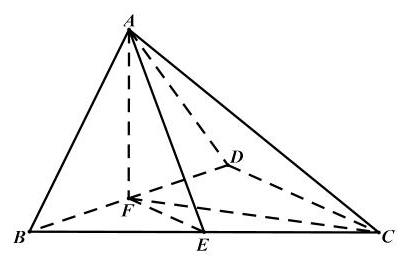
\includegraphics[max width=0.3\textwidth]{images/bo_d7fhnv491nqc73ercsbg_142_1099_1048_402_259_0.jpg}
\end{center}
\hspace*{3em} 

\({BD} \bot  {AF},{BD} \bot  {CF}\) .2 分

所以 \({BD} \bot\) 平面 \({ACF}\) .4 分

所以 \({BD} \bot  {AC}\) .6 分

(2)二面角 \(A - {BD} - C\) 的大小为 \(\frac{\pi }{2}\) ，即平面 \({ABD} \bot\) 平面 \({BCD}\) 由平面 \({ABD} \cap\) 平面 \({BCD} = {BD}\) ,且由( 1 )知 \({AF} \bot  {BD}\) , \({AF} \subset\) 平面 \({ABD}\)

所以 \({AF} \bot\) 平面 \({BCD}\) .8 分

从而 \(\angle {AEF}\) 即为 \({AE}\) 与平面 \({BCD}\) 所成角. 10 分

在 \(R\mathbf{t}{\Delta ABF}\) 中, \({AB} = \sqrt{2},{BD} = 1\) ,从而 \({AF} = 1\)

在 \({\Delta BCD}\) 中, \({EF} = \frac{1}{2}{CD} = 1\)

因为 \({AF} \bot\) 平面 \({BCD}\) ,且 \({EF} \subset\) 平面 \({BCD}\) ,所以 \({AF} \bot  {EF}\)

所以在 \(R\mathbf{t}{\Delta AEF}\) 中, \({AF} \bot  {EF}\) ,且 \({AF} = {EF} = 1\) .12 分

易求得 \(\angle {AEF} = \frac{\pi }{4}\;\) 即 \({AE}\) 与平面 \({BCD}\) 所成角的大小为 \(\frac{\pi }{4}\) .14 分

3. (2025 高三二模松江 18)已知梯形 \({PBCD}\) 中， \({PD}//{BC},E\) 为 \({PD}\) 上的一点且

\({BE} \bot  {PD},{PE} = {BE} = 1,{BC} = \frac{1}{2}{ED}\) ,将 \(\bigtriangleup {PBE}\) 沿 \({BE}\) 翻折使得二面角 \(P - {BE} - C\) 的平面角为 \(\theta\) ,连接 \({PC}\text{ 、 }{PD},F\) 为棱 \({PD}\) 的中点.

(1)求证: \({FC}//\) 平面 \({PBE}\) ；

(2)当 \(\theta  = \frac{2\pi }{3}\) 时，求直线 \({FC}\) 和平面 \({BCDE}\) 所成角的大小.

\begin{center}
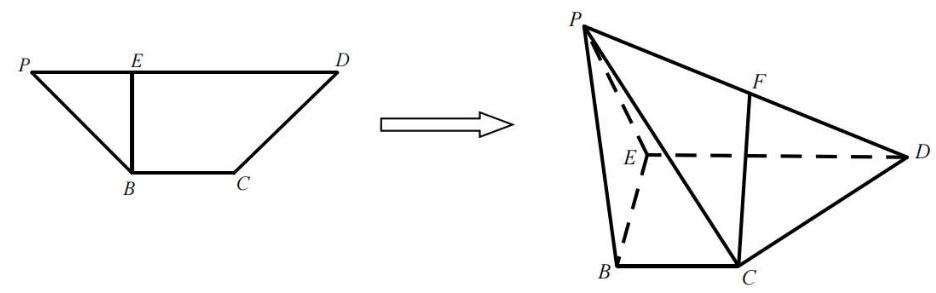
\includegraphics[max width=0.8\textwidth]{images/bo_d7fhnv491nqc73ercsbg_143_265_352_936_293_0.jpg}
\end{center}
\hspace*{3em} 

【答案】(1)证明见解析; (2) \(\arcsin \frac{\sqrt{15}}{10}\) .

【解析】(1) 取 \({ED}\) 的中点 \(M\) ,连接 \({CM}\text{ 、 }{FM}\) ,

因为点 \(F\) 为棱 \({PD}\) 的中点,且 \({BC} = \frac{1}{2}{ED}\) ,所以 \({FM}//{PE}\) 且 \({CM}//{BE}\) ,

\({FM}//{PE},{FM} \text{ ⊄ }\) 平面 \({PBE},{PE} \subset\) 平面 \({PBE}\) ,

所以 \({FM}//\) 平面 \({PBE}\) ,同理可得 \({CM}//\) 平面 \({PBE}\) . ...2 分

因为 \({FM} \subset\) 平面 \({CFM},{CM} \subset\) 平面 \({CFM}\) ,且 \({FM} \cap  {CM} = M\) ,

所以平面 \({CFM}//\) 平面 \({PBE}\) . ...2 分

因为 \({FC} \subset\) 平面 \({CFM}\) ,所以 \({FC}//\) 平面 \({PBE}\) . ...2 分

(2)过点 \(F\) 作 \({FH} \bot  {ED}\) 于点 \(H\) ，连接 \({CH}\) ，

因为 \({BE} \bot  {PE}\) , \({BE} \bot  {DE}\) , \({PE} \cap  {DE} = E,{PE},{DE} \subset\) 平面 \({PDE}\) ,

因为 \({BE} \bot\) 平面 \({PDE}\) ,所以 \({BE} \bot  {FH}\) ,

因为 \({BE} \subset\) 平面 \({BCDE}\) , \({ED} \subset\) 平面 \({BCDE}\) ,且 \({BE} \cap  {ED} = E\) ,

所以 \({FH} \bot\) 平面 \({BCDE}\) . ...2 分

所以 \(\angle {FCH}\) 就是直线 \({FC}\) 和平面 \({BCDE}\) 所成角.

由题意得:二面角 \(P - {BE} - C\) 的平面角为 \(\angle {PED} = \frac{2\pi }{3}\) ，

由( 1 )易得 \(\angle {FMD} = \frac{2\pi }{3}\) ，

在 Rt \(\bigtriangleup {FHM}\) 中,由 \(\angle {FMH} = \frac{\pi }{3},{FM} = \frac{1}{2}\) ,得 \({FH} = \frac{\sqrt{3}}{4}\) , 取 \({PE}\) 中点为 \(G\) ,连接 \({BG}\) ,

第 5 页(共 31 页)

因为 \(G,F\) 分别为 \({PE},{PD}\) 的中点,

所以 \({GF}//{ED}\) ,且 \({GF} = \frac{1}{2}{ED}\) ,又 \({BC} = \frac{1}{2}{ED}\) ,

所以四边形 \({BCFG}\) 为平行四边形,所以 \({BG} = {CF}\) ,

在 Rt \({\Delta BEG}\) 中,由 \({EG} = \frac{1}{2},{BE} = 1\) ，得 \({BG} = \frac{\sqrt{5}}{2}\) ，则 \({CF} = \frac{\sqrt{5}}{2}\) . ...2 分

在 Rt \({\Delta FHC}\) 中,由 \(\sin \angle {FCH} = \frac{FH}{FC} = \frac{\sqrt{15}}{10}\) ,得 \(\angle {FCH} = \arcsin \frac{\sqrt{15}}{10}\) ,

即得直线 \({FC}\) 和平面 \({BCDE}\) 所成角为 \(\arcsin \frac{\sqrt{15}}{10}\) . ...2 分

4.(2025 高三二模浦东 18)如图，四边形 \({ABCD}\) 为长方形， \({PA} \bot\) 平面 \({ABCD}\) ， \({AB} = {AP} = 2,{AD} = 3.\)

(1)若 \(E\text{ 、 }F\) 分别是 \({PB}\text{ 、 }{CD}\) 的中点，求证: \({EF}//\) 平面 \({PAD}\) ；

(2)边 \({BC}\) 上是否存在点 \(G\) ，使得直线 \({PG}\) 与平面 \({PAD}\) 所成的角的大小为 \({30}^{ \circ  }\) ？若存在， 求 \({BG}\) 长; 若不存在,说明理由.

\begin{center}
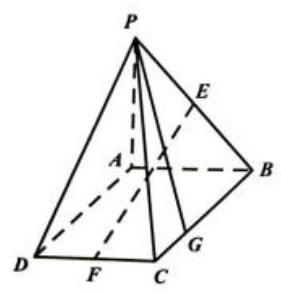
\includegraphics[max width=0.2\textwidth]{images/bo_d7fhnv491nqc73ercsbg_144_252_1090_281_293_0.jpg}
\end{center}
\hspace*{3em} 

【答案】(1)见解析; (2) 存在, \({BG} = 2\sqrt{2}\)

【解析】法一: (1) 证明: 取 \({AP}\) 中点 \(G\) ,连接 \({EG}\text{ 、 }{DG},\because {GE}//{AB},{DF}//{AB}\) ,

\(\therefore {GE}//{DF},\because {GE} = \frac{1}{2}{AB},{DF} = \frac{1}{2}{AB},\therefore {GE} = {DF}\) ，

\(\therefore\) 四边形 \({DFEG}\) 为平行四边形, \(\therefore {EF}//{DG}\) ,

\(\because {DG} \subset\) 平面 \({PDA}\) ， \({EF}\) 在平面 \({PDA}\) 外，

\(\therefore {EF}//\) 平面 \({PDA}\) .

(2)作 \({GH}\bot {AD}\) ，垂足为 \(H\) ，连接 \({PH}\) ， \(\because {PA}\bot\) 平面 \({ABCD}\) ，

\(\therefore {PA} \bot  {GH}\) ， \(\therefore {GH} \bot\) 平面 \({PAD}\) ， \(\therefore\) 直线 \({PG}\) 与平面 \({PAD}\) 所成的角为 \(\angle {GPH} = {30}^{ \circ  }\) ， \(\therefore \frac{HG}{PH} = \tan {30}^{ \circ  } = \frac{1}{\sqrt{3}},\therefore {PH} = 2\sqrt{3},\therefore {BG} = {AH} = \sqrt{P{H}^{2} - P{A}^{2}} = 2\sqrt{2}\) ,

\(\therefore\) 边 \({BC}\) 上存在点 \(G\) ,使得直线 \({PG}\) 与平面 \({PAD}\) 所成的角为 \({30}^{ \circ  },{BG} = 2\sqrt{2}\) .

\begin{center}
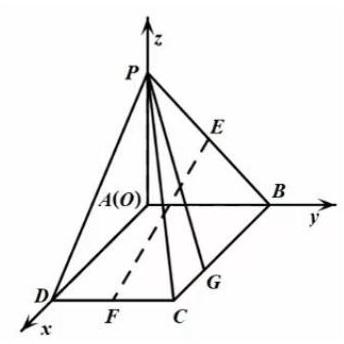
\includegraphics[max width=0.2\textwidth]{images/bo_d7fhnv491nqc73ercsbg_145_1117_222_344_344_0.jpg}
\end{center}
\hspace*{3em} 

法二: (1) 证: 如图建立空间直角坐标,则 \(D\left( {3,0,0}\right) ,B\left( {0,2,0}\right)\) , \(P\left( {0,0,2}\right) ,F\left( {3,1,0}\right) ,E\left( {0,1,1}\right) ,C\left( {3,2,0}\right) ,\therefore \overrightarrow{EF} = \left( {3,0, - 1}\right)\) , 取平面 \({PAD}\) 的法向量 \(\overrightarrow{n} = \left( {0,1,0}\right)\) ，

\(\because \overrightarrow{EF} \cdot  \overrightarrow{n} = 0\) ,且 \({EF}\) 在平面 \({PDA}\) 外, \(\therefore {EF}//\) 平面 \({PDA}\)

(2)设 \({BG} = t\left( {0 \leq  t \leq  3}\right)\) ，则 \(G\left( {t,2,0}\right)\) ， \(\therefore \overrightarrow{PG} = \left( {t,2, - 2}\right)\) ， 取平面 \({PAD}\) 的法向量 \(\overrightarrow{n} = \left( {0,1,0}\right)\) ，设 \(\overrightarrow{PG}\) 与 \(\overrightarrow{n}\) 的夹角为 \(\varphi\) ，

则 \(\sin {30}^{ \circ  } = \left| {\cos \varphi }\right|  = \frac{2}{\sqrt{{t}^{2} + 8}}\) ,求得 \(t = 2\sqrt{2}\) ,

\(\therefore\) 边 \({BC}\) 上存在点 \(G\) ,使得直线 \({PG}\) 与平面 \({PAD}\) 所成的角为 \({30}^{ \circ  },{BG} = 2\sqrt{2}\) .

四、二面角

1. (2025 高三二模宝山 12)空间中有相互垂直的两条异面直线 \({l}_{1}\text{ 、 }{l}_{2}\) ，点

\(A\text{ 、 }B \in  {l}_{1},C\text{ 、 }D \in  {l}_{2}\) ,且 \({AB} = 4,{CD} = 1\) ,若 \({DA} \bot  {DB}\) ,且 \({AC} = {BC} + 2\) ,则二面角 \(D - {AB} - C\) 平面角的余弦值最小为\_\_\_\_\_.

\begin{center}
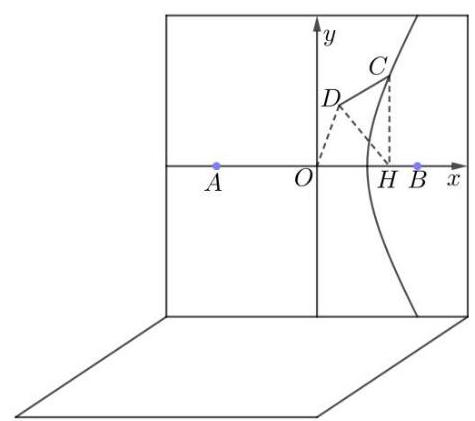
\includegraphics[max width=0.4\textwidth]{images/bo_d7fhnv491nqc73ercsbg_145_1026_1251_475_421_0.jpg}
\end{center}
\hspace*{3em} 

【答案】 \(\frac{4\sqrt{3}}{9}\)

【解析】以 \({AB}\) 中点为原点， \({AB}\) 为 \(x\) 轴， \({AB}\) 的垂直平分线为 \(y\) 轴建立直角坐标系,如图所示, \(A\left( {-2,0}\right) ,B\left( {2,0}\right)\) 由 \({AC} = {BC} + 2\) ,可知点 \(C\) 在双曲线 \({x}^{2} - \frac{{y}^{2}}{3} = 1\left( {x \geq  1}\right)\) 上, 过点 \(C\) 作 \({CH} \bot  {AB}\) ,交 \({AB}\) 于 \(H\) ,

因为 \({AB} \bot  {CD}\) , \({AB} \bot  {CH}\) ,所以 \({AB} \bot\) 平面 \({DCH}\) ,所以 \({AB} \bot  {DH}\) , 所以 \(\angle {DHC}\) 即为二面角 \(D - {AB} - C\) 的平面角,

因为 \({DA} \bot  {DB}\) ,所以 \({DO} = \frac{1}{2}{AB} = 2\) ,

设 \(C\left( {{x}_{0},{y}_{0}}\right)\) ,则 \({DH} = \sqrt{4 - {x}_{0}^{2}}\) ,

\(\cos \angle {DHC} = \frac{D{H}^{2} + C{H}^{2} - C{D}^{2}}{{2DH} \cdot  {CH}} = \frac{4 - {x}_{0}^{2} + {y}_{0}^{2} - 1}{2\sqrt{4 - {x}_{0}^{2}} \cdot  \left| {y}_{0}\right| } \; = \frac{{x}_{0}^{2}}{\sqrt{\left( {4 - {x}_{0}^{2}}\right)  \cdot  \left( {3{x}_{0}^{2} - 3}\right) }} = \sqrt{\frac{1}{-{12}{\left( \frac{1}{{x}_{0}^{2}} - \frac{5}{8}\right) }^{2} + \frac{27}{16}}} \geq  \frac{4\sqrt{3}}{9}\) ,当 \({x}_{0}^{2} = \frac{8}{5}\) 时,等号成立.

2. (2025 高三二模闵行 17) 如图,在四棱锥 \(P - {ABCD}\) 中,底面 \({ABCD}\) 为长方形,

\begin{center}
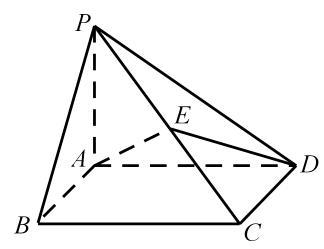
\includegraphics[max width=0.2\textwidth]{images/bo_d7fhnv491nqc73ercsbg_146_1064_448_324_249_0.jpg}
\end{center}
\hspace*{3em} 

\({PA} \bot\) 底面 \({ABCD},E\) 是 \({PC}\) 中点,已知

\({AB} = 2,{AD} = 2\sqrt{2},{PA} = 2\) .

(1)证明: \({AD}\bot {BP}\) ；

(2)求二面角 \(E - {AD} - B\) 的大小.

【答案】(1)证明见解析；(2) \(\frac{\pi }{4}\)

【解析】(1) 证明: 因为 \({PA} \bot\) 底面 \({ABCD}\) ,所以 \({AP} \bot  {AD}\) , 又因为 \({ABCD}\) 为长方形，所以 \({AB} \bot  {AD}\) ， 2 分

而 \({AP}\) 和 \({AB}\) 是平面 \({PAB}\) 上的两条相交直线，所以 \({AD} \bot\) 平面 \({PAB}\) ， .4 分

又 \({BP} \subset\) 平面 \({PAB}\) ,所以 \({AD} \bot  {BP}\) ; 6 分

(2)以 \(A\) 为原点，直线 \({AB}\) 为 \(x\) 轴，直线 \({AD}\) 为 \(y\) 轴，直线 \({AP}\) 为 \(z\) 轴建立直角坐标系. 由题平面 \({ABCD}\) 的一个法向量为 \(\left( {0,0,1}\right)\) , 8 分

且 \(A\left( {0,0,0}\right) ,D\left( {0,2\sqrt{2},0}\right) ,E\left( {1,\sqrt{2},1}\right)\) ,

设平面 \({EAD}\) 的法向量 \(\overrightarrow{n} = \left( {x,y,z}\right)\) ,则 \(\left\{  \begin{array}{l} 2\sqrt{2}y = 0, \\  x + \sqrt{2}y + z = 0, \end{array}\right.\)

可取 \(x = 1\) ,解得 \(y = 0,z =  - 1\) ,从而可得平面 \({EAD}\) 的一个法向量 \(\overrightarrow{n} = \left( {1,0, - 1}\right) ,\ldots {10}\) 分记二面角 \(E - {AD} - B\) 的大小为 \(\theta \left( {0 < \theta  < \frac{\pi }{2}}\right)\) ,则 \(\cos \theta  = \left| \frac{-1}{\sqrt{2} \times  1}\right|  = \frac{\sqrt{2}}{2}\) ,解得 \(\theta  = \frac{\pi }{4}\) , 所以二面角 \(E - {AD} - B\) 的大小为 \(\frac{\pi }{4}\) . .14 分

3. (2025 高三二模徐汇 17)如图， \({ABCD} - {A}_{1}{B}_{1}{C}_{1}{D}_{1}\) 是一块正四棱台形铁料，上、下底面的边长分别为 \({20}\mathrm{\;{cm}}\) 和 \({40}\mathrm{\;{cm}}\) ,高 \({30}\mathrm{\;{cm}}\) .

\begin{center}
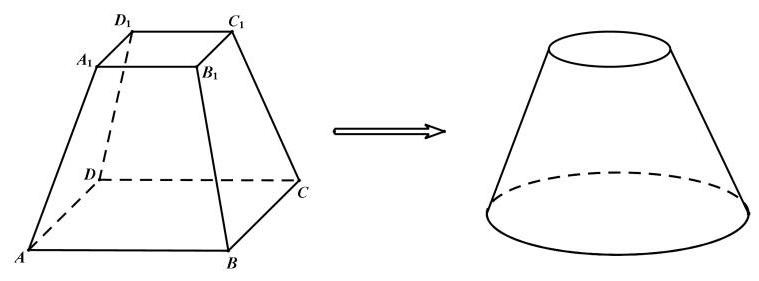
\includegraphics[max width=0.6\textwidth]{images/bo_d7fhnv491nqc73ercsbg_146_257_1816_759_281_0.jpg}
\end{center}
\hspace*{3em} 

第 8 页(共 31 页)

(1)求正四棱台 \({ABCD} - {A}_{1}{B}_{1}{C}_{1}{D}_{1}\) 的侧面 \({BC}{C}_{1}{B}_{1}\) 与底面 \({ABCD}\) 所成二面角的大小；

(2)现削去部分铁料(不计损耗)，将原正四棱台打磨为一个圆台，使得该圆台的上、下底面分别为原正四棱台上、下底面正方形的内切圆及其内部. 求削去部分与原正四棱台的体积之比.

【答案】(1) \(\arctan 3;\;\) (2) \(\frac{4 - \pi }{4}\)

【解析】(1) 设正方形 \({ABCD},{A}_{1}{B}_{1}{C}_{1}{D}_{1}\) 的中心分别为 \(O,{O}_{1}\) ,连接 \(O{O}_{1}\) ,则 \(O{O}_{1} \bot\) 平面 \({ABCD}\) .

分别取 \({BC},{B}_{1}{C}_{1}\) 的中点 \(E,{E}_{1}\) ,连接 \(E{E}_{1},{OE},O{E}_{1}\) ,则 \({OE} \bot  {BC},{O}_{1}{E}_{1} \bot  {B}_{1}{C}_{1}\) . 又 \(E,{E}_{1}\) 分别为等腰梯形 \({BC}{C}_{1}{B}_{1}\) 底边 \({BC},{B}_{1}{C}_{1}\) 的中点,所以 \(E{E}_{1} \bot  {BC}\) .

由 \({O}_{1}{E}_{1}//{A}_{1}{B}_{1}//{AB}//{OE}\) 可得四边形 \({O}_{1}{OE}{E}_{1}\) 是一个直角梯形.

\(E{E}_{1} \bot  {BC}\) ,又 \({OE} \bot  {BC},\angle {OE}{E}_{1}\) 为侧面 \({BC}{C}_{1}{B}_{1}\) 与底面 \({ABCD}\) 所成二面角的平面角. 由条件知 \({O}_{1}{E}_{1} = \frac{1}{2}{A}_{1}{B}_{1} = {10},{OE} = \frac{1}{2}{AB} = {20},O{O}_{1} = {30}\) , 所以 \(\tan \angle {OE}{E}_{1} = \frac{O{O}_{1}}{{OE} - {O}_{1}{E}_{1}} = \frac{30}{10} = 3\) . 所以侧面 \({BC}{C}_{1}{B}_{1}\) 与底面 \({ABCD}\) 所成二面角的大小为 \(\arctan 3\)

(2)设圆台 \(O - {O}_{1}\) 上底面圆半径 \(r = {10}\mathrm{\;{cm}}\) ，下底面圆半径 \(R = {20}\mathrm{\;{cm}}\) ，高 \({O}_{1}O = {30}\mathrm{\;{cm}}\) ，

则圆台 \(O - {O}_{1}\) 的体积为 \({V}_{1} = \frac{1}{3}\pi \left( {{10}^{2} + {20}^{2} + {10} \times  {20}}\right)  \times  {30} = {7000\pi }\left( {\mathrm{{cm}}}^{3}\right)\) .

又正四棱台的体积 \({V}_{2} = \frac{1}{3}\left( {{20}^{2} + {40}^{2} + \sqrt{{20}^{2} \times  {40}^{2}}}\right)  \times  {30} = {28000}\left( {\mathrm{\;{cm}}}^{3}\right)\) ,

所以削去部分的体积 \({V}_{3} = {28000} - {7000\pi }\left( {\mathrm{{cm}}}^{3}\right)\) ,

所以削去部分与正四棱台的体积之比为 \(\frac{{28000} - {7000\pi }}{28000} = \frac{4 - \pi }{4}\) .

\begin{center}
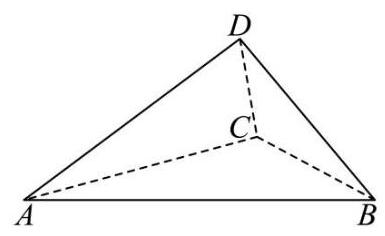
\includegraphics[max width=0.3\textwidth]{images/bo_d7fhnv491nqc73ercsbg_147_1127_1813_385_236_0.jpg}
\end{center}
\hspace*{3em} 

4.(2025 高三二模黄浦 18)在四面体 \({ABCD}\) 中， \({DB} = {DC} = 2\) ， \({DB} \bot  {DC}\) .

(1)若 \(\bigtriangleup  {ABC}\) 为正三角形，平面 \({ABC} \bot\) 平面 \({DBC}\) ，求四面体 \({ABCD}\) 体积;

(2)若 \({AB} = {AC} = 4\) ， \({AD} = 3\) ，求二面角 \(A - {BC} - D\) 的大小.

【答案】(1) \(\frac{2\sqrt{6}}{3};\left( 2\right) \arccos \frac{\sqrt{7}}{4}\)

【解析】(1) 由题设 \(\bigtriangleup {BCD}\) 为等腰直角三角形,且 \({DB} = {DC} = 2,{DB} \bot  {DC}\) ,

所以 \({BC} = 2\sqrt{2}\) ,又 \(\bigtriangleup {ABC}\) 为正三角形,故 \({S}_{\bigtriangleup {ABC}} = \frac{1}{2} \times  {\left( 2\sqrt{2}\right) }^{2} \times  \sin {60}^{ \circ  } = 2\sqrt{3}\) ,

若 \(E\) 为 \({BC}\) 的中点,连接 \({DE}\) ,则 \({DE} \bot  {BC}\) ,又平面 \({ABC} \bot\) 平面 \({DBC}\) ,

平面 \({ABC} \cap\) 平面 \({DBC} = {BC},{DE} \subset\) 平面 \({DBC}\) ,故 \({DE} \bot\) 平面 \({ABC}\) ,

所以 \({DE} = \sqrt{2}\) 是 \(D - {ABC}\) 的高，则其体积 \(V = \frac{1}{3} \cdot  {DE} \cdot  {S}_{\bigtriangleup {ABC}} = \frac{1}{3} \times  \sqrt{2} \times  2\sqrt{3} = \frac{2\sqrt{6}}{3}\) ；

(2)由(1) \({DE}\bot {BC}\) 且 \({BC} = {2\sqrt{2}}\) ， \({DE} = \sqrt{2}\) ，

又 \({AB} = {AC} = 4\) ，则 \({AE} = \sqrt{14}\) ，且 \({AE}\bot {BC}\) ，又 \({AD} = 3\) ， 所以二面角 \(A - {BC} - D\) 的平面角为 \(\angle {DEA}\) ,且 \(\cos \angle {DEA} = \frac{A{E}^{2} + D{E}^{2} - A{D}^{2}}{{2AE} \cdot  {DE}} = \frac{{14} + 2 - 9}{2\sqrt{14} \times  \sqrt{2}} = \frac{\sqrt{7}}{4}\) . 所以二面角大小为 \(\arccos \frac{\sqrt{7}}{4}\) .

\begin{center}
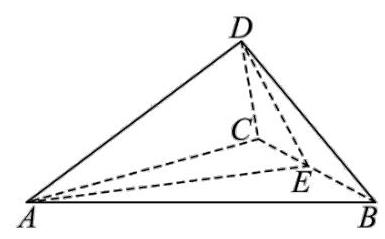
\includegraphics[max width=0.3\textwidth]{images/bo_d7fhnv491nqc73ercsbg_148_1046_819_385_239_0.jpg}
\end{center}
\hspace*{3em} 

\begin{center}
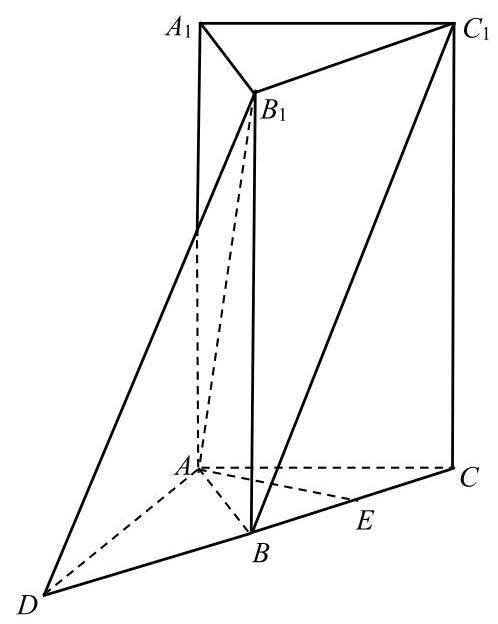
\includegraphics[max width=0.4\textwidth]{images/bo_d7fhnv491nqc73ercsbg_148_1072_1242_498_624_0.jpg}
\end{center}
\hspace*{3em} 

5.(2025 高三二模静安 19)如图，在正三棱柱 \({ABC} - {A}_{1}{B}_{1}{C}_{1}\) 中, \(A{A}_{1} = {2AC} = 4\) ,延长 \({CB}\) 至 \(D\) ,使 \({CB} = {BD},E\) 是线段 \({BC}\) 的中点.

(1)求证: \circled{1} 直线 \({C}_{1}B//\) 平面 \(A{B}_{1}D\) ； \circled{2}  \({AE}\bot {D{B}_{1}}\) .

(2)求二面角 \({B}_{1} - {AD} - C\) 的正弦值.

【答案】(1) 证明见解析; (2) \(\frac{4\sqrt{17}}{17}\)

【解析】(1) 证明:  \circled{1}  由已知,有 \({C}_{1}{B}_{1} = {CB} = {BD}\) ,

\({C}_{1}B//{B}_{1}D\) . 又因为 \({B}_{1}D \subset\) 平面 \(A{B}_{1}D\) ,所以,直线 \({C}_{1}B//\) 平面 \(A{B}_{1}D\) . (4 分)

 \circled{2} 由已知，有 \(B{B}_{1} \bot\) 平面 \({ABC}\) ，

所以直线 \({CD}\) 是直线 \({B}_{1}D\) 在平面 \({ABC}\) 内的射影.

又因为 \(E\) 是线段 \({CD}\) 的中点, \(\bigtriangleup {ABC}\) 是全等三角形,有 \({AE} \bot  {CD}\) .

再由三垂线定理,得 \({AE} \bot  D{B}_{1}\) . (4 分)

(2)解 1:取 \({AD}\) 的中点 \(F\) ，由于 \({BD} = {BA}\) ，

有 \({BF} \bot  {AD}\) ， \({BF} = 1\) ，

所以， \(\angle {B}_{1}{FB}\) 是二面角 \({B}_{1} - {AD} - C\) 的平面角. (3 分)

\begin{center}
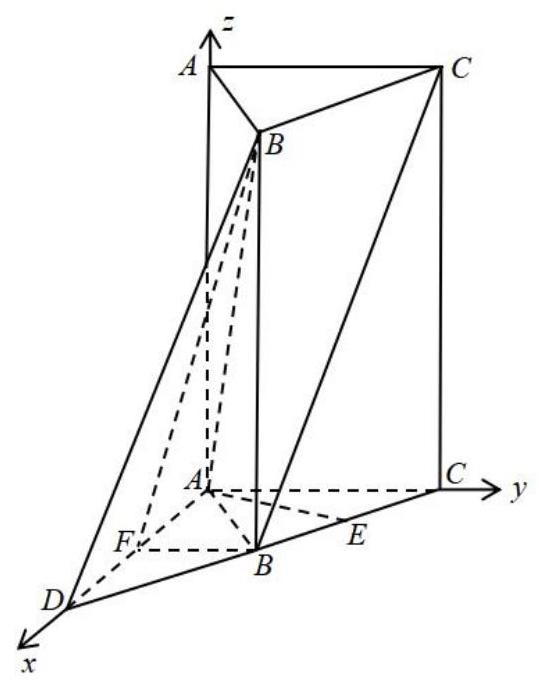
\includegraphics[max width=0.4\textwidth]{images/bo_d7fhnv491nqc73ercsbg_149_1026_649_539_683_0.jpg}
\end{center}
\hspace*{3em} 

故,二面角 \({B}_{1} - {AD} - C\) 的大小为 \(\arctan 4\) .

所以,二面角 \({B}_{1} - {AD} - C\) 的正弦值为 \(\frac{4\sqrt{17}}{17}\) (3 分)

解 2: 在 \(\bigtriangleup {ACD}\) 中,由于 \({CB} = {BD} = {BA}\) ,

所以 \(\angle {DAC} = {90}^{ \circ  }\) .

以点 \(A\) 为原点,建立空间直角坐标系 \(O - {xyz}\) ,(1 分)

则 \(A\left( {0,0,0}\right) \text{ 、 }{B}_{1}\left( {\sqrt{3},1,4}\right) \text{ 、 }D\left( {2\sqrt{3},0,0}\right)\) ,

\(\overrightarrow{AD} = \left( {2\sqrt{3},0,0}\right) ,\)

\(\overrightarrow{A{B}_{1}} = \left( {\sqrt{3},1,4}\right)\) . (2分)

设平面 \(A{B}_{1}D\) 的法向量 \(\overrightarrow{n} = \left( {x,y,z}\right)\) ,则

\(\left\{  {\begin{array}{l} \overrightarrow{n} \cdot  \overrightarrow{AD} = 0, \\  \overrightarrow{n} \cdot  \overrightarrow{A{B}_{1}} = 0, \end{array}\text{ 即 }\left\{  \begin{array}{l} 2\sqrt{3}x = 0, \\  \sqrt{3}x + y + {4z} = 0, \end{array}\right. }\right.\) 所以 \(\left\{  \begin{array}{l} x = 0, \\  y =  - {4z}, \end{array}\right.\) 所以 \(\overrightarrow{n} = \left( {0, - 4,1}\right)\) .

取平面 \({ACB}\) 的法向量 \(\overrightarrow{m} = \left( {0,0,1}\right)\) ,则 \(\cos \langle \overrightarrow{n},\overrightarrow{m}\rangle  = \frac{\overrightarrow{n} \cdot  \overrightarrow{m}}{\left| \overrightarrow{n}\right| \left| \overrightarrow{m}\right| } = \frac{1}{\sqrt{17}}\) ,

所以，二面角 \({B}_{1} - {AD} - C\) 的正弦值为 \(\frac{4\sqrt{17}}{17}\) . (3 分)

\section*{五、点到直线、平面的距离}

1. (2025 高三二模徐汇 6)已知 \({PA}\bot\) 平面 \({ABC},{\Delta ABC}\) 是直角三角形，且 \({AB} = {AC} = 2\) ， \({PA} = 4\) ，则点 \(P\) 到直线 \({BC}\) 的距离是\_\_\_\_\_.

【答案】 \(3\sqrt{2}\)

【解析】作 \({AD} \bot  {BC}\) 交 \({BC}\) 于 \(D\) ,连接 \({PD}\) ,因为 \(\bigtriangleup {ABC}\) 是直角三角形,

第11页(共 31页)

\(\therefore {AD} = \frac{1}{2}{BC} = \frac{1}{2}\sqrt{{2}^{2} + {2}^{2}} = \sqrt{2}\) ,

因为 \({PA} \bot\) 平面 \({ABC},{PD}\) 在平面 \({ABC}\) 内的射影为 \({AD}\) ,则由三垂线定理可得

\({PD} \bot  {BC}\) ,则点 \(P\) 到直线 \({BC}\) 的距离是 \(\sqrt{{4}^{2} + {\sqrt{2}}^{2}} = 3\sqrt{2}\) .

2. (2025 高三二模黄浦 9)某商场要悬挂一个棱长为 2 米的正方体物体作为装饰物，如图， \(A,B,C,D\) 为该正方体的顶点， \(B{B}_{1}\text{ 、 }C{C}_{1}\text{ 、 }D{D}_{1}\) 为三根直绳索，且均垂直于屋顶所在的平面 \(\alpha\) . 若平面 \({BCD}\) 与平面 \(\alpha\) 平行,且点 \(A\) 到 \(\alpha\) 的距离为 2 米,则直绳索 \(B{B}_{1}\) 的长度约为\_\_\_\_\_米. (结果精确到 0.01 米)

\begin{center}
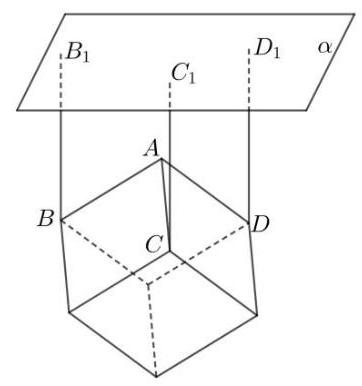
\includegraphics[max width=0.3\textwidth]{images/bo_d7fhnv491nqc73ercsbg_150_293_688_362_386_0.jpg}
\end{center}
\hspace*{3em} 

【答案】3.15

【解析】由题意,直绳索 \(B{B}_{1}\) 的长度即为点 \(A\) 到 \(\alpha\) 的距离加上点 \(A\) 到平面 \({BCD}\) 的距离, 三棱锥 \(A - {BCD}\) 为正三棱锥,底面是边长为 \(2\sqrt{2}\) 的正三角形,侧棱两两垂直且长度为 2, 过点 \(A\) 向平面 \({BCD}\) 作垂线,垂足为 \(O,O\) 为 \({\Delta BCD}\) 的中心,则 \({BO} = \frac{2\sqrt{6}}{3}\) ,所以 \({AO} = \sqrt{A{B}^{2} - B{O}^{2}} = \frac{2\sqrt{3}}{3},\)

所以 \(B{B}_{1} = 2 + \frac{2\sqrt{3}}{3} \approx  {3.15}\) 米.

3.(2025 高三二模黄浦 16)给定四面体 \({ABCD}\) . 平面 \(\alpha\) 满足: \circled{1}  \(A\) 、 \(B\) 、 \(C\) 、 \(D\) 四个点均不在平面 \(\alpha\) 上,也不在 \(\alpha\) 的同侧;  \circled{2} 若平面 \(\alpha\) 与四面体 \({ABCD}\) 的棱有公共点,则该公共点一定是此棱的中点或两个三等分点之一. 设 \(A\text{ 、 }B\text{ 、 }C\text{ 、 }D\) 四个点到平面 \(\alpha\) 的距离分别为 \({d}_{i}\left( {i = 1,2,3,4}\right)\) ,那么 \({d}_{i}\) 的所有不同值的个数组成的集合为( )

A. \(\{ 1,2,3,4\}\) B. \(\{ 1,2,3\}\) C. \(\{ 1,2\}\) D. \(\{ 1\}\)

【答案】B

【解析】当平面 \(\alpha\) 与四面体 \({ABCD}\) 的三条棱的中点相交时,四个点到平面 \(\alpha\) 的距离相同,

此时 \({d}_{i}\) 只有一个 1 个值;

当平面 \(\alpha\) 经过四面体 \({ABCD}\) 的棱 \({AB}\) 的中点,且经过棱 \({AC},{AD}\) 靠近点 \(A\) 的三等分点时,

\(C,D\) 到平面 \(\alpha\) 的距离相等， \(A,B\) 到平面 \(\alpha\) 的距离相等，且两距离不等，故此时 \({d}_{i}\) 的所有不同值的个数为 2 ;

当平面 \(\alpha\) 经过四面体 \({ABCD}\) 的棱 \({AB}\) 的中点,且经过棱 \({AC}\) 靠近点 \(A\) 的三等分点,经过棱 \({AD}\) 靠近点 \(D\) 的三等分点时, \(A,B\) 到平面 \(\alpha\) 的距离相等, \(A,C,D\) 到平面 \(\alpha\) 的距离均不等

故此时 \({d}_{i}\) 的所有不同值的个数为 3 ;

若 \({d}_{i}\) 的所有不同值的个数为 4,则平面 \(\alpha\) 不能经过各棱中点,只经过各棱三等分点,但若只经过三等分点,则必然经过靠近同一顶点的三等分点,此时必有两顶点到平面 \(\alpha\) 距离相等,故 \({d}_{i}\) 的所有不同值的个数不可能是 4 ;

所以 \({d}_{i}\) 的所有不同值的个数组成的集合为 \(\{ 1,2,3\}\) ,故选 B.

4.(2025 高三二模崇明 17)如图，在四棱锥 \(P - {ABCD}\) 中，底面 \({ABCD}\) 是边长为 2 的正方形，且 \({CB}\bot {BP},{CD}\bot {DP},{PA} = 2\) ，点 \(E,F\) 分别为 \({PB},{PD}\)

\begin{center}
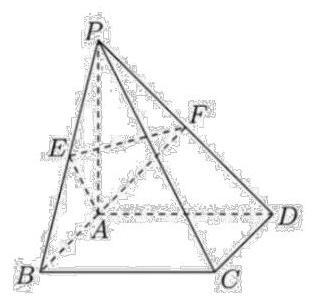
\includegraphics[max width=0.2\textwidth]{images/bo_d7fhnv491nqc73ercsbg_151_1175_1218_309_300_0.jpg}
\end{center}
\hspace*{3em} 

的中点.

(1)求证: \({PA}\bot\) 平面 \({ABCD}\) ；

(2)求点 \(P\) 到平面 \({AEF}\) 的距离.

【答案】(1)证明见解析；(2) \(\frac{2\sqrt{3}}{3}\)

【解析】(1) 证明: 由题意, \({CB} \bot  {AB}\) ,又

\({CB} \bot  {BP},{AB} \cap  {BP} = B,{AB},{BP} \subset\) 平面 \({ABP}\) ，于是 \({CB} \bot\) 平面 \({ABP}\) ，

而 \({PA} \subset\) 平面 \({ABP}\) ,则 \({CB} \bot  {PA}\) , .4 分

同理 \({CD} \bot  {PA}\) ,

又 \({CB} \cap  {CD} = C,{CB},{CD} \subset\) 平面 \({ABCD}\) ,

所以 \({PA} \bot\) 平面 \({ABCD}\) . .7 分

(2)由(1)得 \({PA} \bot  {AB}\) ，

在 Rt \({\Delta PAB}\) 中，点 \(E\) 为 \({PB}\) 的中点， \({AE} = \sqrt{2}\) ，同理 \({AF} = \sqrt{2}\) ，

在 \(\bigtriangleup  {PBD}\) 中， \({EF} = \frac{1}{2}{BD} = \sqrt{2}\) ，因此 \({S}_{\bigtriangleup {AEF}} = \frac{1}{2} \times  \sqrt{2} \times  \sqrt{2} \times  \frac{\sqrt{3}}{2} = \frac{\sqrt{3}}{2}\) ，

在直角 \({\Delta PAB}\) 中, \({S}_{\bigtriangleup {APE}} = \frac{1}{2} \times  \frac{1}{2} \times  2 \times  2 = 1\) , 3 分

由( 1 )知 \({CB}\bot\) 平面 \({ABP}\) ，则 \({AD}\bot\) 平面 \({ABP}\) ，

于是点 \(F\) 到平面 \({APE}\) 的距离为 \(\frac{1}{2}{AD} = 1\) ，

设点 \(P\) 到平面 \({AEF}\) 的距离为 \(h\) ,

由 \({V}_{P - {AEF}} = {V}_{F - {AEP}}\) ,得 \(\frac{1}{3} \times  \frac{\sqrt{3}}{2} \times  h = \frac{1}{3} \times  1 \times  1\) ,解得 \(h = \frac{2\sqrt{3}}{3}\) ,

所以点 \(P\) 到平面 \({AEF}\) 的距离为 \(\frac{2\sqrt{3}}{3}\) .7 分

5.(2025 高三二模虹口 17)如图所示，在四棱锥 \(P - {ABCD}\) 中， \({PA}\bot\) 平面 \({ABCD}\) ， \({AB} \bot  {AD},{AD}//{BC},{AB} = {BC} = 2,{AD} = 4\) .

(1)求证:平面 \({PAC} \bot\) 平面 \({PCD}\) ；

(2)若异面直线 \({PB}\) 和 \({CD}\) 所成角为 \(\frac{\pi }{3}\) ，求点 \(B\) 到平面 \({PCD}\) 的距离.

\begin{center}
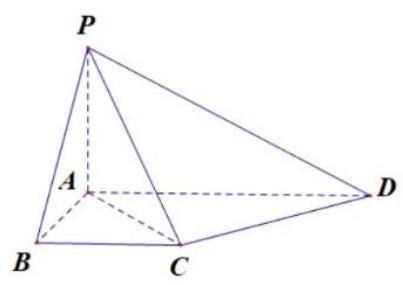
\includegraphics[max width=0.3\textwidth]{images/bo_d7fhnv491nqc73ercsbg_152_241_1081_403_285_0.jpg}
\end{center}
\hspace*{3em} 

第 17 题图

【答案】(1)证明见解析；(2) \(\frac{\sqrt{6}}{3}\)

【解析】(1) \({AC} = {CD} = 2\sqrt{2}\) ，所以 \(A{C}^{2} + C{D}^{2} = A{D}^{2}\) ，故 \({AC}\bot {CD}\) . . .2 分

由 \({PA} \bot\) 平面 \({ABCD}\) , \({CD}\) 在平面 \({ABCD}\) 上,所以 \({PA} \bot  {CD}\) . .4 分

由于 \({AC}\) 与 \({PA}\) 是平面 \({PAC}\) 上的两条相交直线,所以 \({CD} \bot\) 平面 \({PAC}\) .

由于 \({CD}\) 在平面 \({PCD}\) 上,所以平面 \({PAC} \bot\) 平面 \({PCD}\) . .6 分

(2)以点 \(A\) 为原点，分别以 \(\overrightarrow{AB}\text{ 、 }\overrightarrow{AD}\text{ 、 }\overrightarrow{AP}\) 为 \(x\text{ 、 }y\text{ 、 }z\) 轴的正方向建立直角坐标系. 设 \(P\left( {0,0,h}\right)\) ,则 \(\overrightarrow{PB} = \left( {2,0, - h}\right) ,\overrightarrow{CD} = \left( {-2,2,0}\right)\) , .8 分

所以 \(\cos \frac{\pi }{3} = \frac{\left| \overrightarrow{PB} \cdot  \overrightarrow{CD}\right| }{\left| \overrightarrow{PB}\right|  \cdot  \left| \overrightarrow{CD}\right| } = \frac{4}{\sqrt{4 + {h}^{2}} \times  2\sqrt{2}} = \frac{1}{2}\) .

解得 \(h = 2\) . 10 分

\(\overrightarrow{PC} = \left( {2,2, - 2}\right) ,\overrightarrow{PB} = \left( {2,0, - 2}\right)\) ,设 \(\overrightarrow{n} = \left( {x,y,z}\right)\) 为平面 \({PCD}\) 的一个法向量,

则 \(\left\{  \begin{array}{l} \overrightarrow{n} \cdot  \overrightarrow{PC} = 0, \\  \overrightarrow{n} \cdot  \overrightarrow{CD} = 0. \end{array}\right.\) 即 \(\left\{  \begin{array}{l} {2x} + {2y} - {2z} = 0, \\   - {2x} + {2y} = 0. \end{array}\right.\) 取 \(y = 1\) ,可得 \(\overrightarrow{n} = \left( {1,1,2}\right)\) . .12 分

故点 \(B\) 到平面 \({PCD}\) 的距离 \(d = \frac{\left| \overrightarrow{PB} \cdot  \overrightarrow{n}\right| }{\left| \overrightarrow{n}\right| } = \frac{2}{\sqrt{6}} = \frac{\sqrt{6}}{3}\) . .14 分

\begin{center}
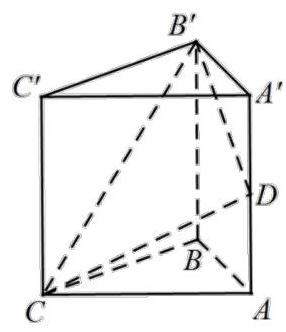
\includegraphics[max width=0.2\textwidth]{images/bo_d7fhnv491nqc73ercsbg_153_1206_802_286_332_0.jpg}
\end{center}
\hspace*{3em} 

6. (2025 高三二模长宁 18) 如图,在直三棱柱 \({ABC} - {A}^{\prime }{B}^{\prime }{C}^{\prime }\) 中， \({AB}\bot {AC}\) ， \({AC} = {AB} = 2,A{A}^{\prime } = 2\sqrt{2}\) ,点 \(D\) 是棱 \(A{A}^{\prime }\) 的中点.

(1)求证:平面 \({CD}{B}^{\prime } \bot\) 平面 \({CB}{B}^{\prime }{C}^{\prime }\) ；

(2)求点 \({C}^{\prime }\) 到平面 \({CD}{B}^{\prime }\) 的距离以及三棱锥 \({C}^{\prime } - {CD}{B}^{\prime }\) 的体积.

【答案】(1)证明见解析;

(2)点 \({C}^{\prime }\) 到平面 \({CD}{B}^{\prime }\) 的距离为 2，三棱锥 \({C}^{\prime } - {CD}{B}^{\prime }\) 的体积为 \(\frac{4}{3}\sqrt{2}\)

【解析】(1) 连结 \(B{C}^{\prime }\) ,与 \(C{B}^{\prime }\) 交于点 \(O\) ,

因为点 \(D\) 是棱 \(A{A}^{\prime }\) 的中点,所以 \({AD} = {A}^{\prime }D = \sqrt{2}\) ,

因为 \({ABC} - {A}^{\prime }{B}^{\prime }{C}^{\prime }\) 是直三棱柱,

所以 \(A{A}^{\prime } \bot\) 面 \({ABC},C{C}^{\prime } \bot\) 面 \({ABC}\) ,四边形 \({C}^{\prime }{CB}{B}^{\prime }\) 是平行四边形,

从而 \(A{A}^{\prime } \bot  {AC},A{A}^{\prime } \bot  {AB}\) ,所以 \({CD} = {B}^{\prime }D = \sqrt{6}\) ,

\begin{center}
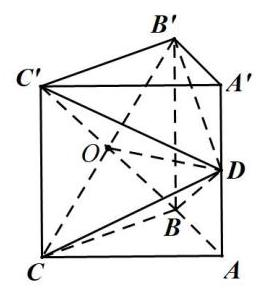
\includegraphics[max width=0.2\textwidth]{images/bo_d7fhnv491nqc73ercsbg_153_1229_1610_256_290_0.jpg}
\end{center}
\hspace*{3em} 

因为 \({AB} \bot  {AC},{AC} = {AB} = 2\) ,所以 \({CB} = A{A}^{\prime } = C{C}^{\prime } = 2\sqrt{2}\) ,即有四边形 \({C}^{\prime }{CB}{B}^{\prime }\) 是正方形,

所以 \(C{B}^{\prime } = {C}^{\prime }B\) ,且互相平分,从而有

\({DO} \bot  C{B}^{\prime },\) 2 分

同理 \({DO} \bot  {C}^{\prime }B\) ,

\(C{B}^{\prime }\) 与 \({C}^{\prime }B\) 相交于点 \(O\) ,所以 \({DO} \bot\) 平面

\({C}^{\prime }{CB}{B}^{\prime }\) , 2 分

\({DO} \subset\) 平面 \({CD}{B}^{\prime }\) ,所以平面 \({CD}{B}^{\prime } \bot\) 平面

\({C}^{\prime }{CB}{B}^{\prime }\) ; .2 分

第 15页(共 31页)

(2)因为平面 \({CD}{B}^{\prime } \bot\) 平面 \({C}^{\prime }{CB}{B}^{\prime }\) ，平面 \({CD}{B}^{\prime } \cap\) 平面 \({C}^{\prime }{CB}{B}^{\prime } = C{B}^{\prime }\) ，

由四边形 \({C}^{\prime }{CB}{B}^{\prime }\) 是正方形，可得 \({C}^{\prime }O \bot  C{B}^{\prime }\) ,

所以 \({C}^{\prime }O \bot\) 平面 \({CD}{B}^{\prime }\) , .2 分

所以点 \({C}^{\prime }\) 到平面 \({CD}{B}^{\prime }\) 的距离 \({C}^{\prime }O = 2\) , .2 分

\(\cos \angle {CD}{B}^{\prime } = \frac{6 + 6 - {16}}{2 \times  6} =  - \frac{1}{3},\)

所以 \({S}_{{CD}{B}^{\prime }} = \frac{1}{2} \times  \sqrt{6} \times  \sqrt{6} \times  \frac{2\sqrt{2}}{3} = 2\sqrt{2}\) , .2 分

三棱锥 \({C}^{\prime } - {CD}{B}^{\prime }\) 的体积 \(V = \frac{1}{3} \times  2\sqrt{2} \times  2 = \frac{4}{3}\sqrt{2}\) .2 分

或建系

\begin{center}
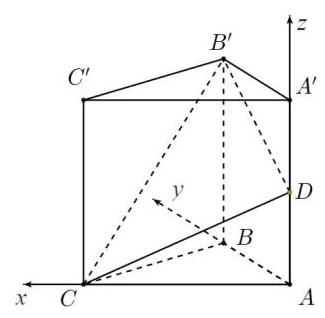
\includegraphics[max width=0.2\textwidth]{images/bo_d7fhnv491nqc73ercsbg_154_1186_774_325_318_0.jpg}
\end{center}
\hspace*{3em} 

(1)如图，建立空间直角坐标系，则

\(A\left( {0,0,0}\right) ,B\left( {0,2,0}\right) ,D\left( {0,0,\sqrt{2}}\right) ,C\left( {2,0,0}\right) ,{B}^{\prime }\left( {0,2,2\sqrt{2}}\right) ,\)

\({C}^{\prime }\left( {2,0,2\sqrt{2}}\right) ,\)

\(\overrightarrow{C{B}^{\prime }} = \left( {-2,2,2\sqrt{2}}\right) ,\overrightarrow{C{C}^{\prime }} = \left( {0,0,2\sqrt{2}}\right) ,\overrightarrow{CD} = \left( {-2,0,\sqrt{2}}\right)\) ,

平面 \({CB}{B}^{\prime }{C}^{\prime }\) 的法向量 \(\overrightarrow{n} = \left( {1,1,0}\right)\) , .2 分

平面 \(C{B}^{\prime }D\) 的法向量

\(\overrightarrow{m} = \left( {1, - 1,\sqrt{2}}\right) ,\) .2 分

\(\overrightarrow{m} \cdot  \overrightarrow{n} = 1 - 1 = 0,\)

所以平面 \({CB}{B}^{\prime }{C}^{\prime } \bot\) 平面 \(C{B}^{\prime }D\) ; .2 分

(2)点 \({C}^{\prime }\) 到平面 \({CD}{B}^{\prime }\) 的距离 \(d = \frac{\left| \overrightarrow{C{C}^{\prime }} \cdot  \overrightarrow{m}\right| }{\left| \overrightarrow{m}\right| } = \frac{4}{2} = 2\) ， .4 分体积的解法同上.

\begin{center}
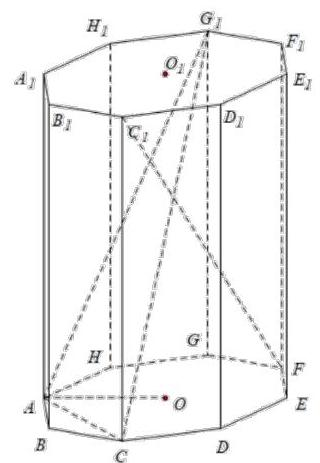
\includegraphics[max width=0.2\textwidth]{images/bo_d7fhnv491nqc73ercsbg_154_1245_1698_320_463_0.jpg}
\end{center}
\hspace*{3em} 

第 18 题

7.(2025 高三二模杨浦 18)座落于杨浦滨江的世界技能博物馆由百年历史文化保护建筑改建而成, 其中的支柱保留了原有的正八棱柱, 既考虑了结构力学优势, 又体现了对历史建筑的尊重和传承.

如图, \({O}_{1}\text{ 、 }O\) 分别为正八棱柱的上下两个底面的中心,已知 \({OA} = 1\) , \(A{A}_{1} = 4\) .

(1)求证: \({BC} \bot  {C}_{1}F\) ；

第 16页(共 31页)

(2)求点 \(O\) 到平面 \({AC}{G}_{1}\) 的距离.

【答案】(1)证明见解析; (2) \(\frac{2}{3}\)

【解析】(1)连结 \({CF}\) ,由底面为正八边形可知, \({BC} \bot  {CF}\) .3 因为 \(C{C}_{1} \bot\) 底面 \({ACG}\) ,所以 \({CF}\) 是 \({C}_{1}F\) 在底面 \({ACG}\) 的射影,

所以 \({BC} \bot  {C}_{1}F\) .6

(2)连结 \({OC}\) 、 \({O{G}_{1}}\) 、 \({AG}\) ，

\({S}_{\bigtriangleup {OAC}} = \frac{1}{2}{OA} \times  {OC} = \frac{1}{2},{V}_{{G}_{1} - {OAC}} = \frac{1}{3} \times  {S}_{\bigtriangleup {OAC}} \times  G{G}_{1} = \frac{1}{3} \times  \frac{1}{2} \times  4 = \frac{2}{3}\) , .8

由 \(\angle {GAC} = {45}^{ \circ  } + {45}^{ \circ  } = {90}^{ \circ  }\) ,可知 \({AG} \bot  {AC}\) ,

由 \(G{G}_{1} \bot\) 平面 \({ACG}\) 可知 \({AG}\) 是 \(A{G}_{1}\) 在平面的射影,故 \(A{G}_{1} \bot  {AC}\) ,

\({AC} = \sqrt{{1}^{2} + {1}^{2}} = \sqrt{2},\;A{G}_{1} = \sqrt{{\left( \sqrt{2}\right) }^{2} + {4}^{2}} = 3\sqrt{2},\)

\({S}_{\bigtriangleup {AC}{G}_{1}} = \frac{1}{2}{AC} \times  A{G}_{1} = \frac{1}{2} \times  \sqrt{2} \times  3\sqrt{2} = 3,\) .11

设点 \(O\) 到平面 \({AC}{G}_{1}\) 的距离为 \(d\) ,则 \(\frac{1}{3} \times  {S}_{\bigtriangleup {AC}{G}_{1}} \times  d = {V}_{{G}_{1} - {OAC}}\) ,计算得 \(d = \frac{2}{3}\) . .14 另解:

(1)以 \(O\) 为原点，分别以 \(\overrightarrow{OC}\) 、 \(\overrightarrow{OE}\) 、 \(\overrightarrow{O{O}_{1}}\) 为 \(x\) 轴、 \(y\) 轴、 \(z\) 轴的正方向建立空间直角坐标系. 由 \(B\left( {\frac{\sqrt{2}}{2}, - \frac{\sqrt{2}}{2},0}\right) ,C\left( {1,0,0}\right)\) ,得 \(\overrightarrow{BC} = \left( {1 - \frac{\sqrt{2}}{2},\frac{\sqrt{2}}{2},0}\right)\) , .3

由 \({C}_{1}\left( {1,0,4}\right) ,F\left( {-\frac{\sqrt{2}}{2},\frac{\sqrt{2}}{2},0}\right)\) ,可得 \(\overrightarrow{{C}_{1}F} = \left( {-\frac{\sqrt{2}}{2} - 1,\frac{\sqrt{2}}{2}, - 4}\right)\) ,

由 \(\overrightarrow{BC} \cdot  \overrightarrow{{C}_{1}F} = 0\) ,可知 \({BC} \bot  {C}_{1}F\) .6

(2)由 \(A\left( {0, - 1,0}\right)\) ， \(C\left( {1,0,0}\right)\) ， \({G}_{1}\left( {-1,0,4}\right)\) ，可得 \(\overrightarrow{AC} = \left( {1,1,0}\right)\) ， \(\overrightarrow{A{G}_{1}} = \left( {-1,1,4}\right)\) ， .8 设平面 \({AC}{G}_{1}\) 的法向量为 \(\overrightarrow{n} = \left( {u,v,w}\right)\) ,由 \(\overrightarrow{n} \cdot  \overrightarrow{AC} = 0\) 且 \(\overrightarrow{n} \cdot  \overrightarrow{A{G}_{1}} = 0\) ,

可得 \(\left\{  \begin{array}{l} u + v = 0 \\   - u + v + {4w} = 0 \end{array}\right.\) ,即 \(\left\{  \begin{array}{l} u =  - v \\  v =  - {2w} \end{array}\right.\) ,

取 \(w = 1\) ，可得平面 \({AC}{G}_{1}\) 的一个法向量为 \(\overrightarrow{n} = \left( {2, - 2,1}\right)\) ， .11

设点 \(O\) 到平面 \({AC}{G}_{1}\) 的距离为 \(d\) ,由 \(\overrightarrow{OC} = \left( {1,0,0}\right)\) ,则 \(d = \frac{\left| \overrightarrow{n} \cdot  \overrightarrow{OC}\right| }{\left| \overrightarrow{n}\right| } = \frac{\left| 2 \times  1\right| }{\sqrt{{2}^{2} + {2}^{2} + {1}^{2}}} = \frac{2}{3}\ldots\) . .14

8.(2025 高三二模金山 18)如图，在四棱锥 \(P - {ABCD}\) 中， \({PA}\bot\) 平面 \({PBC}\) ， \({AB} = {2DC} = 4,{BC} = 2\sqrt{2},{AB} \bot  {BC},{DC}//{AB}\) .

\begin{center}
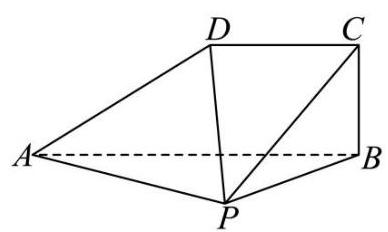
\includegraphics[max width=0.3\textwidth]{images/bo_d7fhnv491nqc73ercsbg_156_983_262_388_232_0.jpg}
\end{center}
\hspace*{3em} 

第 18 题 图

(1)证明:平面 \({ABCD} \bot\) 平面 \({PAB}\) ；

(2)若 \(\angle {ABP} = \frac{\pi }{3}\) ，求点 \(C\) 到平面 \({PAD}\) 的距离.

【答案】(1)证明见解析；(2) \(\frac{2\sqrt{2}}{3}\)

【解析】(1)由 \({PA} \bot\) 平面 \({PBC}\) ， \({BC} \subset\) 平面 \({PBC}\) ，则 \({PA} \bot  {BC}\) ，. 又 \({AB} \bot  {BC}\) ,由 \({PA} \cap  {AB} = A\) 且都在平面 \({PAB}\) 内,则 \({BC} \bot\) 平面 \({PAB},\ldots\) 4 分又 \({BC} \subset\) 面 \({ABCD}\) ,所以平面 \({ABCD} \bot\) 平面 \({PAB}\) . 6 分

(2)法一:由(1)易知 \({PA} \bot  {PB}\) ，又 \(\angle {ABP} = \frac{\pi }{3}\) ，过 \(P\) 作 \({PO} \bot  {AB}\) 于 \(O\) ，

由平面 \({ABCD} \bot\) 平面 \({PAB}\) ，平面 \({ABCD} \cap\) 平面 \({PAB} = {AB}\) ， \({PO} \subset\) 平面 \({PAB}\) ， 所以 \({PO} \bot\) 平面 \({ABCD}\) ,过 \(O\) 作 \({Oz}//{BC}\) ,易知 \({Oz} \bot  {AB}\) , \(\;\ldots \ldots 8\) 分故建立如下图示空间直角坐标系,又 \({AB} = {2DC} = 4,{BC} = 2\sqrt{2},{DC}//{AB}\) ,

\begin{center}
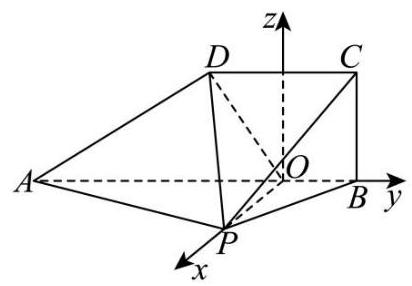
\includegraphics[max width=0.3\textwidth]{images/bo_d7fhnv491nqc73ercsbg_156_299_957_412_286_0.jpg}
\end{center}
\hspace*{3em} 

则 \(A\left( {0, - 3,0}\right) ,P\left( {\sqrt{3},0,0}\right) ,C\left( {0,1,2\sqrt{2}}\right) ,D\left( {0, - 1,2\sqrt{2}}\right)\) ,

所以 \(\overrightarrow{AP} = \left( {\sqrt{3},3,0}\right) ,\overrightarrow{AD} = \left( {0,2,2\sqrt{2}}\right) ,\overrightarrow{DC} = \left( {0,2,0}\right)\) , 10 分

设 \(\overrightarrow{m} = \left( {x,y,z}\right)\) 是平面 \({PAD}\) 的一个法向量,则 \(\left\{  \begin{array}{l} \overrightarrow{m} \cdot  \overrightarrow{AP} = \sqrt{3}x + {3y} = 0 \\  \overrightarrow{m} \cdot  \overrightarrow{AD} = {2y} + 2\sqrt{2}z = 0 \end{array}\right.\) ,

令 \(z =  - 1\) ,则 \(\overrightarrow{m} = \left( {-\sqrt{6},\sqrt{2}, - 1}\right)\) , 12 分

所以点 \(C\) 到平面 \({PAD}\) 的距离 \(\frac{\left| \overrightarrow{m} \cdot  \overrightarrow{DC}\right| }{\left| \overrightarrow{m}\right| } = \frac{2\sqrt{2}}{3}\) . 14 分

法二: 由(1)易知 \({PA} \bot  {PB}\) ,又 \(\angle {ABP} = \frac{\pi }{3}\) ,过 \(P\) 作 \({PO} \bot  {AB}\) 于 \(O\) , 由平面 \({ABCD} \bot\) 平面 \({PAB}\) ,平面 \({ABCD} \cap\) 平面 \({PAB} = {AB},{PO} \subset\) 平面 \({PAB}\) , 所以 \({PO} \bot\) 平面 \({ABCD}\) 8 分

\begin{center}
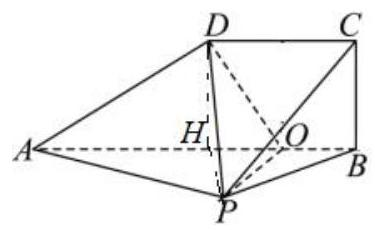
\includegraphics[max width=0.3\textwidth]{images/bo_d7fhnv491nqc73ercsbg_156_324_1903_375_230_0.jpg}
\end{center}
\hspace*{3em} 

第 18页(共 31页)

过 \(D\) 作 \({DH} \bot  {AB}\) 于 \(H\) ,连接 \({PH}\) 易得 \({DH}//{BC},{DH} = {BC} = 2\sqrt{2}\)

因为 \(\angle {ABP} = \frac{\pi }{3},{PA} \bot\) 平面 \({PBC}\) ,

所以 \({PA} \bot  {PB}\) ,又 \({AB} = 4\) ,所以, \({PB} = 2,{AP} = 2\sqrt{3},{PH} = 2\) ,

\({DP} = 2\sqrt{3} = {AD} = {AP},\) 10 分

设 \(C\) 到平面 \({PAD}\) 的距离为 \(d\) ,

\({V}_{C - {ADP}} = {V}_{P - {ADC}},\)

即 \(\frac{1}{3} \times  \frac{\sqrt{3}}{4} \times  {\left( 2\sqrt{3}\right) }^{2} \cdot  d = \frac{1}{3} \times  \frac{1}{2} \times  2 \times  2\sqrt{2} \times  \sqrt{3},d = \frac{2\sqrt{2}}{3}\)

所以点 \(C\) 到平面 \({PAD}\) 距离为 \(\frac{2\sqrt{2}}{3}\) . .14 分

\section*{六、柱体、锥体、球、台体}

1.(2025 高三二模闵行 4)已知圆柱的底面半径为 \(\sqrt{3}\) ，高为 3 ，则圆柱的体积为\_\_\_\_\_.

【答案】 \({9\pi }\)

【解析】圆柱的体积为 \(V = \pi {r}^{2}h = \pi  \times  {\sqrt{3}}^{2} \times  3 = {9\pi }\) .

2.(2025 高三二模虹口 4)若某圆柱的底面半径为 1，母线长为 2，则其侧面积为\_\_\_\_\_.(结果保留 \(\pi\) )

【答案】 \({4\pi }\)

【解析】侧面积为 \({2\pi rh} = {2\pi } \times  1 \times  2 = {4\pi }\) .

3.(2025 高三二模金山 7)已知圆锥底面半径为 1，高为 \(\sqrt{3}\) ，则过圆锥的母线的截面面积的最大值为\_\_\_\_\_.

【答案】 \(\sqrt{3}\)

【解析】由题意知圆锥轴截面的顶角一半的正切值为 \(\tan \alpha  = \frac{1}{\sqrt{3}} = \frac{\sqrt{3}}{3} \Rightarrow  \alpha  = \frac{\pi }{6}\) ,

则轴截面的顶角为 \(\frac{\pi }{3}\) ,则过圆锥母线的截面中轴截面的面积最大,最大面积为 \(\frac{1}{2} \times  2 \times  \sqrt{3} = \sqrt{3}\)

4.(2025 高三二模普陀 8)若一个圆锥的高为 \(\sqrt{2}\) ，侧面积为 \(2\sqrt{2}\pi\) ，则该圆锥侧面展开图中扇形的中心角的大小为\_\_\_\_\_.

【答案】 \(\sqrt{2}\pi\)

【解析】设圆锥的高 \(h = \sqrt{2}\) ,底面半径为 \(r\) ,母线长为 \(l\) ,则 \({l}^{2} = {r}^{2} + {h}^{2}\) ,

\({S}_{\text{ 侧 }} = {\pi rl} = {\pi r}\sqrt{{r}^{2} + 2} = 2\sqrt{2}\pi  \Rightarrow  r = \sqrt{2}\) ,则 \(l = 2\) ,母线即为侧面展开图扇形的半径, 圆锥底面周长 \(c = {2\pi r} = 2\sqrt{2}\pi\) ，即为侧面展开图扇形的弧长，

所以 \(\alpha  = \frac{c}{l} = \frac{2\sqrt{2}\pi }{2} = \sqrt{2}\pi\) .

5.(2025 高三二模宝山 8)已知圆柱的底面积为 \({9\pi }\) ，侧面积为 \({18\pi }\) ，则该圆柱的体积为\_\_\_\_\_.

【答案】 \({27\pi }\)

【解析】设圆柱底面半径为 \(r\) ,高为 \(h\) ,则 \(\left\{  {\begin{array}{l} \pi {r}^{2} = {9\pi } \\  {2\pi rh} = {18\pi } \end{array} \Rightarrow  \left\{  \begin{array}{l} r = 3 \\  h = 3 \end{array}\right. }\right.\) ,

所以 \(V = \pi {r}^{2}h = {27\pi }\) .

6.(2025 高三二模奉贤 8)抛物线 \({x}^{2} = {4y}\) 的准线与圆 \({x}^{2} + {y}^{2} = {r}^{2}\) 相切，将圆绕直径所在直线旋转一周形成一个几何体，则该几何体的表面积为\_\_\_\_\_.

【答案】 \({4\pi }\)

【解析】由题意知准线方程为 \(y =  - 1\) ,则 \(r = 1\) ,又旋转所成的几何体为球,且球的半径为 1,则球的表面积为 \({4\pi } \times  {1}^{2} = {4\pi }\) .

\begin{center}
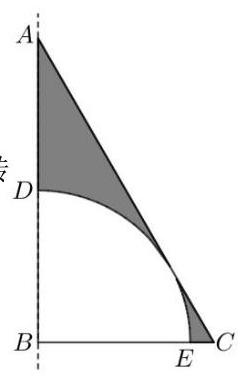
\includegraphics[max width=0.2\textwidth]{images/bo_d7fhnv491nqc73ercsbg_158_1346_1121_242_377_0.jpg}
\end{center}
\hspace*{3em} 

第 10 题图

7.(2025 高三二模杨浦 10)如图，点 \(D,E\) 分别是直角三角形 \({ABC}\) 边 \({AB},{AC}\) 上的点， 斜边 \({AC}\) 与扇形个弧 \({DE}\) 相切，已知 \({AC} = 4,{BC} = 2\) ，则阴影部分绕直线 \({AB}\) 旋转一周所形成的几何体的体积为\_\_\_\_\_.

【答案】 \(\frac{2\sqrt{3}}{3}\pi\)

【解析】可知,图形绕 \({AB}\) 旋转一周的几何体为一个圆锥的底部挖出一个半球, 连接点 \(B\) 与切点,连线为直角三角形斜边的高,也为扇形的半径,

\({AB} = \sqrt{A{C}^{2} - B{C}^{2}} = 2\sqrt{3}\) ,所以扇形的半径 \(R = \frac{{AB} \cdot  {BC}}{AC} = \sqrt{3}\) ,

圆锥的底面半径 \(r = {BC} = 2\) ,高 \(h = {AB} = 2\sqrt{3}\) ,

所以阴影部分旋转后的体积 \(V = \frac{1}{3}\pi {r}^{2}h - \frac{1}{2} \cdot  \frac{4}{3}\pi {R}^{3} = \frac{2\sqrt{3}}{3}\pi\) .

8.(2025 高三二模松江 10)如图，在三棱锥 \(P - {ABC}\) 中， \({PA},{PB},{PC}\) 两两垂直,且 \({PA} = 3,{PB} = 2,{PC} = 1\) ,设 \(M\) 底面 \({ABC}\) 内一点,定义 \(f\left( M\right)  = \left( {m,n,p}\right)\) ,其中 \(m,n,p\) 分别表示三棱锥 \(M - {PAB}\) ,三棱锥

\begin{center}
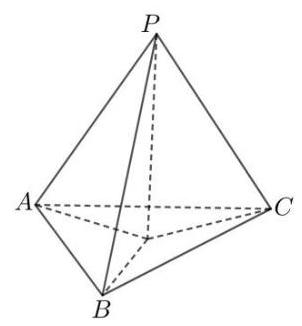
\includegraphics[max width=0.2\textwidth]{images/bo_d7fhnv491nqc73ercsbg_158_1241_1841_302_326_0.jpg}
\end{center}
\hspace*{3em} 

第 20 页(共 31 页)

\(M - {PBC}\) ,三棱锥 \(M - {PCA}\) 的体积. 若 \(f\left( M\right)  = \left( {\frac{2}{3},x,y}\right)\) ,且 \(\frac{a}{x} + \frac{1}{y} \geq  {12}\) 恒成立,则正实数 \(a\) 的最小值为\_\_\_\_\_.

【答案】 1

【解析】已知 \({PA} \bot  {PB},{PA} = 3,{PB} = 2\) ,则 \({S}_{\Delta PAB} = \frac{1}{2} \times  3 \times  2 = 3\) , 因为 \(f\left( M\right)  = \left( {\frac{2}{3},x,y}\right)\) ,所以 \({V}_{M - {PAB}} = \frac{1}{3}{S}_{\Delta PAB} \cdot  {h}_{1} = \frac{2}{3}\left( {h}_{1}\right.\) 为 \(M\) 到平面 \({PAB}\) 的距离), 即 \(\frac{1}{3} \times  3 \cdot  {h}_{1} = \frac{2}{3}\) ,解得 \({h}_{1} = \frac{2}{3}\) ,又 \({V}_{P - {ABC}} = \frac{1}{6}{PA} \cdot  {PB} \cdot  {PC} = \frac{1}{6} \times  3 \times  2 \times  1 = 1\) , 所以 \(x + y + \frac{2}{3} = 1\) ,所以 \(x + y = \frac{1}{3}\) , \(\frac{a}{x} + \frac{1}{y} = 3\left( {\frac{a}{x} + \frac{1}{y}}\right) \left( {x + y}\right)  = 3\left( {a + 1 + \frac{ay}{x} + \frac{x}{y}}\right)  \geq  3\left( {a + 1 + 2\sqrt{a}}\right) ,\) 因为 \(\frac{a}{x} + \frac{1}{y} \geq  {12}\) 恒成立,所以 \(3\left( {a + 1 + 2\sqrt{a}}\right)  \geq  {12}\) ,化简可得 \(\left( {\sqrt{a} + 3}\right) \left( {\sqrt{a} - 1}\right)  \geq  0\) , 所以 \(\sqrt{a} \leq   - 3\) (舍) 或 \(\sqrt{a} \geq  1\) ,解得 \(a \geq  1\) ,所以 \(a\) 的最小值为 1 .

9.(2025 高三二模崇明 14)已知一个圆锥的轴截面是边长为 2 的等边三角形，则这个圆锥的侧面积为( )

A. \({2\pi }\) B. \({3\pi }\) C. \({4\pi }\)

D. \(\frac{\sqrt{3}}{3}\pi\)

【答案】A

【解析】由题意知母线长为 2,半径为 1,则圆锥的侧面积为 \(\pi  \times  2 \times  1 = {2\pi }\) ,故选 A.

\begin{center}
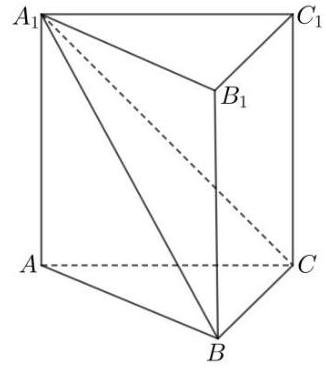
\includegraphics[max width=0.2\textwidth]{images/bo_d7fhnv491nqc73ercsbg_159_1059_1498_326_371_0.jpg}
\end{center}
\hspace*{3em} 

10. (2025 高三二模松江 15)在三棱柱 \({ABC} - {A}_{1}{B}_{1}{C}_{1}\) 中， \({AB} = A{A}_{1} = 1\) ,动点 \(P\) 满足 \(\overrightarrow{BP} = \lambda \overrightarrow{BC} + \overrightarrow{B{B}_{1}},\lambda  \in  \left( {0,1}\right)\) , 则下列几何体体积为定值的是( )

A. 四棱锥 \(P - {A}_{1}{AB}{B}_{1}\;\) B. 四棱锥 \(P - {A}_{1}{AC}{C}_{1}\)

C. 三棱锥 \(P - {A}_{1}B{C}_{1}\;\) D. 三棱锥 \(P - {A}_{1}{BC}\)

【答案】D

【解析】动点 \(P\) 满足 \(\overrightarrow{BP} = \lambda \overrightarrow{BC} + \overrightarrow{B{B}_{1}},\lambda  \in  \left( {0,1}\right)\) ,即 \(\overrightarrow{BP} - \overrightarrow{B{B}_{1}} = \overrightarrow{{B}_{1}P} = \lambda \overrightarrow{BC}\) ,则点 \(P\) 在线段 \({B}_{1}{C}_{1}\) 上,

因为 \({B}_{1}{C}_{1}//{BC},{BC} \subset\) 平面 \({A}_{1}{BC},{B}_{1}{C}_{1}\) 不在平面 \({A}_{1}{BC}\) ,所以 \({B}_{1}{C}_{1}//\) 平面 \({A}_{1}{BC}\) , 所以点 \(P\) 到平面 \({A}_{1}{BC}\) 的距离 \(d\) 为定值，

\({V}_{P - {A}_{1}{BC}} = \frac{1}{3} \cdot  {S}_{\Delta {A}_{1}{BC}} \cdot  d\) ,面积和距离均为定值,故选 D.

\begin{center}
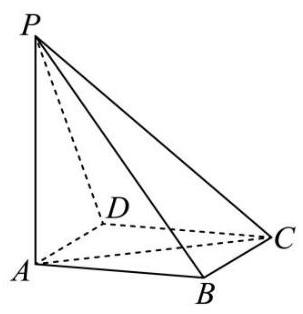
\includegraphics[max width=0.2\textwidth]{images/bo_d7fhnv491nqc73ercsbg_160_1269_464_303_314_0.jpg}
\end{center}
\hspace*{3em} 

11. (2025 高三二模嘉定 17)如图，在四棱锥 \(P - {ABCD}\) 中， \({PA}\bot\) 平面 \({ABCD}\) ， \({PA} = {AC} = 2,{BC} = 1,{AB} = \sqrt{3}.\)

(1)若 \({AD}//\) 平面 \({PBC}\) ，证明: \({AD} \bot  {PB}\) ；

(2)在我国古代数学典籍《九章算术》中，记载了一种特殊的三棱锥——鳖臑, 其四个面均为直角三角形, 找出本题图中的一个鳖臑, 并计算它的体积和表面积.

【答案】(1) 证明见解析; (2) \(P - {ABC}\) 为一个鳖膈，体积为 \(\frac{\sqrt{3}}{3}\) ，表面积为 \(\frac{4 + 3\sqrt{3} + \sqrt{7}}{2}\)

【解析】(1) 由题设 \(B{C}^{2} + A{B}^{2} = A{C}^{2}\) ,则 \({AB} \bot  {BC}\) ,

由 \({PA} \bot\) 平面 \({ABCD}\) , \({BC} \subset\) 平面 \({ABCD}\) ,则 \({PA} \bot  {BC}\) ,

而 \({PA} \cap  {AB} = A\) 都在面 \({PAB}\) 内,则 \({BC} \bot\) 面 \({PAB}\) ,

由 \({AD}//\) 平面 \({PBC},{AD} \subset\) 面 \({ABCD}\) ,面 \({ABCD} \cap\) 面 \({PBC} = {BC}\) ,

所以 \({AD}//{BC}\) ,则 \({AD} \bot\) 面 \({PAB},{PB} \subset\) 面 \({PAB}\) ,故 \({AD} \bot  {PB}\) .

(2)由 \({PA} \bot\) 平面 \({ABCD}\) ， \({AB},{AC} \subset\) 平面 \({ABCD}\) ，则 \({PA} \bot  {AB},{PA} \bot  {AC}\) ，

由(1)知 \({AB}\bot {BC}\) ，且 \({BC}\bot\) 面 \({PAB}\) ， \({PB} \subset\) 面 \({PAB}\) ，则 \({BC}\bot {PB}\) ，

所以 \({\bigtriangleup {PAB}},{\bigtriangleup {PAC}},{\bigtriangleup {ABC}},{\bigtriangleup {PBC}}\) 都是直角三角形，且 \({PB} = \sqrt{7}\) ，

根据题设定义， \(P - {ABC}\) 为一个鳖儒，体积

\(V = \frac{1}{3}{PA} \cdot  \frac{1}{2}{AB} \cdot  {BC} = \frac{1}{3} \times  2 \times  \frac{1}{2} \times  \sqrt{3} \times  1 = \frac{\sqrt{3}}{3},\)

表面积

\[
S = {S}_{\bigtriangleup {PAB}} + {S}_{\bigtriangleup {PAC}} + {S}_{\bigtriangleup {ABC}} + {S}_{\bigtriangleup {PBC}} = \sqrt{3} + 2 + \frac{\sqrt{3}}{2} + \frac{\sqrt{7}}{2} = \frac{4 + 3\sqrt{3} + \sqrt{7}}{2}.
\]

12.(2025 高三二模青浦 18)如图，已知四棱锥 \(S - {ABCD}\) 的底面为菱形， \(\angle {BAD} = \frac{\pi }{3}\) ，

\begin{center}
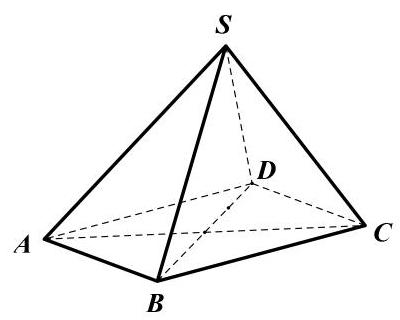
\includegraphics[max width=0.3\textwidth]{images/bo_d7fhnv491nqc73ercsbg_161_1186_306_400_320_0.jpg}
\end{center}
\hspace*{3em} 

\({AS} = {CS}\) .

(1)求证: \({AC}\bot\) 平面 \({BDS}\) ；

(2)若 \({AB} = 2,{BS} = \sqrt{3},{DS} = 1\) ，求四棱锥 \(S - {ABCD}\) 的体积.

【答案】(1)证明见解析; (2) 1

【解析】(1) 记 \({AC} \cap  {BD} = O\) ,连结 \({OS}\) ,

因为 \({AS} = {CS}\) ,所以 \({AC} \bot  {OS}\) ,

由于底面 \({ABCD}\) 为棱形,则 \({AC} \bot  {BD}\) ,

因为 \({BD} \cap  {OS} = O\) ,

所以 \({AC} \bot\) 平面 \({BDS}\) .

(2)由(1)知， \({AO} \bot\) 平面 \({BDS}\) ，

所以， \({V}_{S - {ABCD}} = 2{V}_{S - {ABD}} = 2{V}_{A - {BDS}}\) ，

根据题意,得, \({BD} = 2\) ,

又, \({BS} = \sqrt{3},{DS} = 1\) ,所以 \({BS} \bot  {DS}\) ,

故, \({V}_{A - {BDS}} = \frac{1}{3}{S}_{\Delta BDS} \cdot  {AO} = \frac{1}{2}\) ,所以 \({V}_{S - {ABCD}} = 1\) ,

所以，四棱锥 \(S - {ABCD}\) 的体积为 1 .

七、立体几何应用问题

1. (2025 高三二模静安 9)用总长为 \({14.8}\mathrm{\;m}\) 的钢条制作一个长方体容器的框架，且容器底面的长边比短边长 0.5m (不计损耗).若要使该容器的容积最大，则容器的高为\_\_\_\_\_m.

【答案】 1.2

【解析】设短边长为 \(x\) ,则长边长为 \(x + {0.5}\) ,设高为 \(h\) ,

则 \(4\left( {x + x + {0.5} + h}\right)  = {14.8} \Rightarrow  h = {3.2} - {2x}\left( {0 < x < {1.6}}\right)\) ,

\(\therefore V = x\left( {x + {0.5}}\right) \left( {{3.2} - {2x}}\right)  =  - 2{x}^{3} + {2.2}{x}^{2} + {1.6x}\) ,

\({V}^{\prime } =  - 6{x}^{2} + {4.4x} + {1.6} = 0 \Rightarrow  x = 1,x =  - \frac{4}{15}\) (舍),

当 \(x \in  \left( {0,1}\right)\) 时, \({V}^{\prime } > 0,V\) 单调递增,当 \(x \in  \left( {1,{1.6}}\right)\) 时, \({V}^{\prime } < 0,V\) 单调递减,

则当 \(x = 1\) 时,体积取到最大值,此时 \(h = {3.2} - 2 = {1.2}\) .

2.(2025 高三二模长宁 11)现有一块正四面体木料 \({PABC}\) ，其边长为 3，现需要将木料进行切割,要求切割后底面 \({ABC}\) 上任意一点 \(Q\) 到顶点 \(P\) 的距离不大于 \(\sqrt{7}\) ,则切割好后, 木料体积的最大值是\_\_\_\_\_. (结果保留 \(\pi\) )

【答案】 \(\frac{3\sqrt{2}}{4} + \frac{\sqrt{6}\pi }{6}\)

【解析】设正四面体定点 \(P\) 在底面 \({ABC}\) 的投影为 \(O\) ,则 \(O\) 为正三角形 \({ABC}\) 的中心,

连接 \({OA}\) ,所以 \({AO} = \frac{2}{3} \times  \frac{\sqrt{3}}{2} \times  3 = \sqrt{3},{PO} = \sqrt{P{A}^{2} - A{O}^{2}} = \sqrt{6}\) ,

若底面 \({ABC}\) 上任意一点 \(Q\) 到顶点 \(P\) 的距离不大于 \(\sqrt{7}\) ,

设 \({PQ} = \sqrt{7}\) ,则 \({OQ} = \sqrt{P{Q}^{2} - P{O}^{2}} = 1\) ,

所以以 \(O\) 为圆心,半径为 1 的圆在底面 \(\bigtriangleup {ABC}\) 内的部分为底,以 \(P\) 为顶点的几何体即为符合要求的部分，

如图以 \(O\) 为圆心,半径为 1 的圆与底面 \(\bigtriangleup {ABC}\) 相交的交点为

\begin{center}
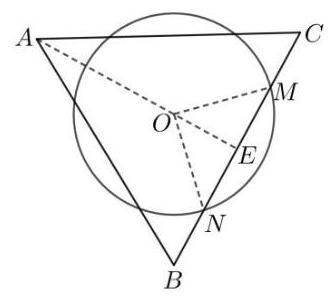
\includegraphics[max width=0.2\textwidth]{images/bo_d7fhnv491nqc73ercsbg_162_1068_891_329_298_0.jpg}
\end{center}
\hspace*{3em} 

\(M,N\) ,

延长 \({OA}\) 交 \({BC}\) 于 \(E\) ,连接 \({OM},{ON}\) ,

所以 \({OE} = \frac{1}{3} \times  \frac{\sqrt{3}}{2} \times  3 = \frac{\sqrt{3}}{2},{OM} = {ON} = 1\) ,

所以 \(\cos \angle {EOM} = \frac{OE}{OM} = \frac{\sqrt{3}}{2}\) ，所以 \(\angle {EOM} = \frac{\pi }{6}\) ，

所以 \(\angle {MON} = \frac{\pi }{3}\) ,所以 \({\Delta MON}\) 为等边三角形,

所以以 \(O\) 为圆心,半径为 1 的圆与底面 \(\bigtriangleup {ABC}\) 内的部分的面积为

\(\pi  \times  {1}^{2} - 3 \times  \left( {\frac{\pi }{6} \times  {1}^{2} - \frac{\sqrt{3}}{4} \times  {1}^{2}}\right)  = \frac{\pi }{2} + \frac{3\sqrt{3}}{4}\) ,

所以切割好后,木料体积的最大值是 \(\frac{1}{3} \times  \left( {\frac{\pi }{2} + \frac{3\sqrt{3}}{4}}\right)  \times  \sqrt{6} = \frac{3\sqrt{2}}{4} + \frac{\sqrt{6}\pi }{6}\) .

\begin{center}
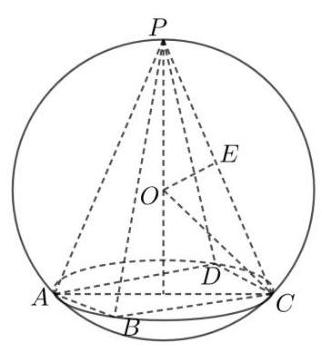
\includegraphics[max width=0.2\textwidth]{images/bo_d7fhnv491nqc73ercsbg_162_1210_1726_322_348_0.jpg}
\end{center}
\hspace*{3em} 

3. (2025 高三二模嘉定 11) 某建筑公司欲设计一个正四棱锥形纪念碑, 要求其顶点位于容积为 \({36\pi }\) 立方米的球形景观灯所在球面上. 考虑到抗风、 抗震等结构安全需求，侧棱长度 \(l\) 需满足 \(2\sqrt{3} \leq  l \leq  3\sqrt{3}\) . 当纪念碑体积取得最大值时，正四棱锥的侧棱长约为\_\_\_\_\_米.(精确到 0.01 米)

【答案】 4.90

【解析】如图,设该球的半径为 \(R\) ,球心为 \(O\) ,正四棱锥的底边长为 \(a\) , 高为 \(h\) ,正四棱锥的侧棱与高所成的角为 \(\theta\) ,则正四棱锥的底边长 \(a = \sqrt{2}l\sin \theta\) ,高 \(h = l\cos \theta\) ,

由题意可得 \({36\pi } = \frac{4}{3}\pi {R}^{3}\) ,解得 \(R = 3\) ,

在 \(\bigtriangleup  {POC}\) 中，作 \({OE}\bot {PC}\) ，垂足为 \(E\) ，

可得 \(\cos \theta  = \frac{\frac{l}{2}}{R} = \frac{l}{6} \in  \left\lbrack  {\frac{\sqrt{3}}{3},\frac{\sqrt{3}}{2}}\right\rbrack\) ,所以 \(l = 6\cos \theta\) ,所以正四棱锥的体积 \(V = \frac{1}{3}{a}^{2}h = \frac{1}{3}{\left( \sqrt{2}l\sin \theta \right) }^{2} \cdot  l\cos \theta  = \frac{2}{3}{\left( 6\cos \theta \right) }^{3}{\sin }^{2}\theta \cos \theta  = {144}{\left( \sin \theta {\cos }^{2}\theta \right) }^{2}\) 设 \(\sin \theta  = t\) ,则 \(t \in  \left\lbrack  {\frac{1}{2},\frac{\sqrt{6}}{3}}\right\rbrack\) ,令 \(y = \sin \theta {\cos }^{2}\theta  = t\left( {1 - {t}^{2}}\right)  = t - {t}^{3}\) ,则 \({y}^{\prime } = 1 - 3{t}^{2}\) , 令 \({y}^{\prime } = 0\) ,解得 \(t = \frac{\sqrt{3}}{3}\) ,当 \(\frac{1}{2} < t < \frac{\sqrt{3}}{3}\) 时, \({y}^{\prime } > 0\) ,当 \(\frac{\sqrt{3}}{3} < t < \frac{\sqrt{6}}{3}\) 时, \({y}^{\prime } < 0\) , 所以函数 \(y = t - {t}^{3}\) 在 \(\left( {\frac{1}{2},\frac{\sqrt{3}}{3}}\right)\) 上严格递增,在 \(\left( {\frac{\sqrt{3}}{3},\frac{\sqrt{6}}{3}}\right)\) 上严格递减, 所以当 \(t = \frac{\sqrt{3}}{3}\) 时， \(y\) 取得最大值 \(\frac{2\sqrt{3}}{9}\) ，则 \({V}_{\max } = {144} \cdot  {\left( \frac{2\sqrt{3}}{9}\right) }^{2} = \frac{64}{3}\) ， 此时 \(\cos \theta  = \sqrt{1 - {\sin }^{2}\theta } = \sqrt{1 - {t}^{2}} = \frac{\sqrt{6}}{3}\) ,则 \(l = 6\cos \theta  = 2\sqrt{6} \approx  {4.90}\) 米.

4.(2025 高三二模奉贤 19)将一块边长为 10 cm 的正方形铁片制作一个正四棱锥的容器罩. 同学们设计了甲、乙、丙三个不同的方案，各自裁下阴影部分，用余下的制作成正四棱锥容器罩，形如最右边的图. 甲和丙是去制作有盖的容器罩，乙是去制作无盖的容器罩. 假设加工过程中铁片损失忽略不计. 设甲、乙、丙中白色的四个等腰三角形的底边分别是 \(x,m\) , \(n\) .

(I) 请你选择其中的某一个方案, 而且只需选一个方案 (选择超过一个方案的, 按第一个方案处理) .你选择的方案是\_\_\_\_\_，求解以下 2 个问题:

(1)求出所选方案相对应的棱锥的侧面积 \(S\left( x\right)\) ， \(S\left( m\right)\) ， \(S\left( n\right)\) ；

(2)求出所选方案相对应棱锥的体积 \(V\left( x\right)\) ， \(V\left( m\right)\) ， \(V\left( n\right)\) 的最大值.

(II) 假设三个方案中相应的体积最大值分别记作 \(V{\left( x\right) }_{\max },V{\left( m\right) }_{\max },V{\left( n\right) }_{\max }\) ，请直接写出三者的大小关系. (不写判断理由与过程)

\begin{center}
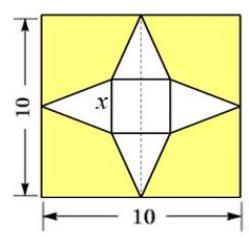
\includegraphics[max width=0.2\textwidth]{images/bo_d7fhnv491nqc73ercsbg_163_245_1728_249_237_0.jpg}
\end{center}
\hspace*{3em} 

甲

\begin{center}
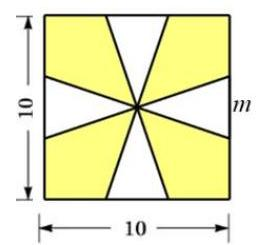
\includegraphics[max width=0.2\textwidth]{images/bo_d7fhnv491nqc73ercsbg_163_520_1721_260_245_0.jpg}
\end{center}
\hspace*{3em} 

乙丙

\begin{center}
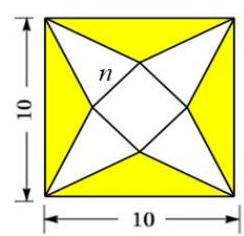
\includegraphics[max width=0.2\textwidth]{images/bo_d7fhnv491nqc73ercsbg_163_798_1731_244_236_0.jpg}
\end{center}
\hspace*{3em} 

\begin{center}
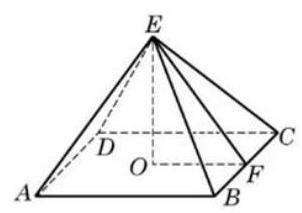
\includegraphics[max width=0.2\textwidth]{images/bo_d7fhnv491nqc73ercsbg_163_1111_1740_302_213_0.jpg}
\end{center}
\hspace*{3em} 

第 19 题图

【答案】(I) 见解析; (II) \({V}_{\max }\left( m\right)  > {V}_{\max }\left( n\right) { > }_{\max }V\left( x\right)\)

【解析】(I) 选择甲方案

(1) \({S}_{\text{ 侧 }}\left( x\right)  = \frac{1}{2}x \cdot  \left( {5 - \frac{x}{2}}\right)  \cdot  4 = {10x} - {x}^{2}\left( {0 < x < {10}}\right)\) 4 分

(2)该正四棱锥的高 \(h\left( x\right)  = \sqrt{{\left( 5 - \frac{x}{2}\right) }^{2} - {\left( \frac{x}{2}\right) }^{2}} = \sqrt{{25} - {5x}}\left( {0 < x < {10}}\right) \;\) 2 分

\(\therefore V\left( x\right)  = \frac{1}{3}{S}_{\text{ 底 }}\left( x\right)  \cdot  h\left( x\right)  = \frac{1}{3}{x}^{2}\sqrt{{25} - {5x}} = \frac{1}{6}\sqrt{{25}{x}^{4} - 5{x}^{5}}\left( {0 < x < {10}}\right) \begin{array}{l}  \\  2\text{ 分 } \end{array}\)

设 \(g\left( x\right)  = {25}{x}^{4} - 5{x}^{5}\left( {0 < x < {10}}\right)\) ,则 \({g}^{\prime }\left( x\right)  = {100}{x}^{3} - {25}{x}^{4}\left( {0 < x < {10}}\right)\)

\(\therefore\) 函数 \(y = g\left( x\right)\) 在区间 \(\left( {0,4}\right)\) 上严格增，在区间 \(\left( {4,{10}}\right)\) 上严格减

\(\therefore\) 当 \(x = 4\) 时, \(V{\left( x\right) }_{\max } = \frac{{16}\sqrt{5}}{3}\) . 5 分

选择乙方案

(1) \({S}_{\text{ 侧 }}\left( x\right)  = \frac{1}{2}m \cdot  5 \cdot  4 = {10m}\left( {0 < m < {10}}\right) \;\) 4 分

(2)该正四棱锥的高 \(h\left( m\right)  = \sqrt{{5}^{2} - {\left( \frac{m}{2}\right) }^{2}} = \sqrt{{25} - \frac{{m}^{2}}{4}}\left( {0 < m < {10}}\right) \;\) 2 分

\(\therefore V\left( x\right)  = \frac{1}{3}{S}_{\text{ 底 }}\left( m\right)  \cdot  h\left( m\right)  = \frac{1}{3}{m}^{2}\sqrt{{5}^{2} - {\left( \frac{m}{2}\right) }^{2}} = \frac{1}{6}\sqrt{{100}{m}^{4} - {m}^{6}}\left( {0 < m < {10}}\right)\) 2 分

设 \(g\left( m\right)  = {100}{m}^{4} - {m}^{6}\left( {0 < m < {10}}\right)\) ,则 \({g}^{\prime }\left( m\right)  = {400}{m}^{3} - 6{m}^{5}\left( {0 < m < {10}}\right)\)

\(\therefore\) 函数 \(y = g\left( m\right)\) 在区间 \(\left( {0,\frac{10}{3}\sqrt{6}}\right)\) 上严格增,在区间 \(\left( {\frac{10}{3}\sqrt{6},{10}}\right)\) 上严格减

\(\therefore\) 当 \(m = \frac{{10}\sqrt{6}}{3}\) 时, \(V{\left( m\right) }_{\max } = \frac{{1000}\sqrt{3}}{27}\) . 5 分

选择丙方案

(1) \(S\left( n\right)  = \frac{1}{2}n\left( {5\sqrt{2} - \frac{n}{2}}\right)  =  - {n}^{2} + {10}\sqrt{2}\left( {0 < n < 5\sqrt{2}}\right) \;\) 4 分

(2)该正四棱锥的高 \(h\left( n\right)  = \sqrt{{\left( 5\sqrt{2} - \frac{n}{2}\right) }^{2} - {\left( \frac{1}{2}n\right) }^{2}} = \sqrt{{50} - 5\sqrt{2n}},\left( {0 < n < 5\sqrt{2}}\right)\) 2 分

\(V\left( n\right)  = \frac{1}{3}{n}^{2}\sqrt{{50} - 5\sqrt{2}n} = \frac{1}{3}\sqrt{{50}{n}^{4} - 5\sqrt{2}{n}^{5}},\left( {0 < n < 5\sqrt{2}}\right) \;2\) 分

\(f\left( n\right)  = {50}{n}^{4} - 5\sqrt{2}{n}^{5},\therefore {f}^{\prime }\left( n\right)  = {400}{n}^{3} - {25}\sqrt{2}{n}^{4}\)

所以函数 \(y = f\left( n\right)\) 在区间 \(\left( {0,4\sqrt{2}}\right)\) 上严格增,在区间 \(\left( {4\sqrt{2},5\sqrt{2}}\right)\) 上严格减

所以当 \(n = 4\sqrt{2}\) 时， \(V{\left( n\right) }_{\max } = \frac{{32}\sqrt{10}}{3}\) 5 分

(II) 甲乙丙中总面积一样, 由于乙的方案是不需要盖, 所以相应的侧面积多了, 因此凭直觉猜想乙的体积最大,可以猜想: \({V}_{\max }\left( m\right)  > {V}_{\max }\left( n\right) { > }_{\max }V\left( x\right)\) 3 分

\section*{八、空间向量}

1. (2025 高三二模徐汇 3) 在空间直角坐标系中,向量 \(\overrightarrow{a} = \left( {-m,6,3}\right) ,\overrightarrow{b} = \left( {2,n,1}\right)\) ,若 \(\overrightarrow{a}//\overrightarrow{b}\) , 则 \(m + n =\) \_\_\_\_\_.

【答案】 -4

【解析】由题意知 \(\frac{-m}{2} = \frac{6}{n} = \frac{3}{1} \Rightarrow  m =  - 6,n = 2 \Rightarrow  m + n =  - 4\) .

2.(2025 高三二模松江 4)已知空间向量 \(\overrightarrow{a} = \left( {2,\lambda ,3}\right) ,\overrightarrow{b} = \left( {-4,2,2}\right)\) ，若 \(\overrightarrow{a}\bot \overrightarrow{b}\) ，则 \(\lambda  =\) \_\_\_\_\_.

【答案】 1

【解析】由题意 \(\overrightarrow{a} \cdot  \overrightarrow{b} = 2 \times  \left( {-4}\right)  + \lambda  \times  2 + 3 \times  2 = 0\) ,解得 \(\lambda  = 1\) .

3. (2025 高三二模浦东 11) 已知 \(\overrightarrow{a},\overrightarrow{b},\overrightarrow{c}\) 为空间中三个单位向量,且 \(\overrightarrow{a} \cdot  \overrightarrow{b} = \overrightarrow{b} \cdot  \overrightarrow{c} = \overrightarrow{c} \cdot  \overrightarrow{a} = 0\) , 若向量 \(\overrightarrow{p}\) 满足 \(\left| {\overrightarrow{p} - 2\overrightarrow{a}}\right|  = \frac{3}{2},\left| {\overrightarrow{p} - 2\overrightarrow{b}}\right|  = \frac{3}{2}\) ，则向量 \(\overrightarrow{p}\) 与向量 \(\overrightarrow{c}\) 夹角的最小值为\_\_\_\_\_. (用反三角表示)

【答案】 \(\arccos \frac{\sqrt{2}}{4}\)

【解析】由题意,设 \(\overrightarrow{a} = \left( {1,0,0}\right) ,\overrightarrow{b} = \left( {0,1,0}\right) ,\overrightarrow{c} = \left( {0,0,1}\right) ,\overrightarrow{p} = \left( {x,y,z}\right)\) ,

\(\left| {\overrightarrow{p} - 2\overrightarrow{a}}\right|  = \frac{3}{2} \Rightarrow  {\left( x - 2\right) }^{2} + {y}^{2} + {z}^{2} = \frac{9}{4}\)  \circled{1} , \(\left| {\overrightarrow{p} - 2\overrightarrow{b}}\right|  = \frac{3}{2} \Rightarrow  {x}^{2} + {\left( y - 2\right) }^{2} + {z}^{2} = \frac{9}{4}\)  \circled{2} ,

 \circled{1} - \circled{2}  \(\Rightarrow  x = y\) ，则 \circled{1} 可化简为 \(2{\left( x - 1\right) }^{2} + {z}^{2} = \frac{1}{4}\) ，

则 \({z}^{2} = \frac{1}{4} - 2{\left( x - 1\right) }^{2} \geq  0\) ,可得 \(x \in  \left\lbrack  {1 - \frac{\sqrt{2}}{4},1 + \frac{\sqrt{2}}{4}}\right\rbrack\) ,

当 \(z > 0\) 时,向量 \(\overrightarrow{p}\) 与向量 \(\overrightarrow{c}\) 夹角可取得最小值,

\(\cos  < \overrightarrow{p},\overrightarrow{c} >  = \frac{\overrightarrow{p} \cdot  \overrightarrow{c}}{\left| \overrightarrow{p}\right| \left| \overrightarrow{c}\right| } = \frac{z}{\sqrt{{x}^{2} + {y}^{2} + {z}^{2}}} = \sqrt{\frac{{z}^{2}}{{x}^{2} + {y}^{2} + {z}^{2}}}\)

\(= \sqrt{\frac{\frac{1}{4} - 2{\left( x - 1\right) }^{2}}{2{x}^{2} + \frac{1}{4} - 2{\left( x - 1\right) }^{2}}} = \sqrt{\frac{-2{x}^{2} + {4x} - \frac{7}{4}}{{4x} - \frac{7}{4}}}\) ,

令 \(t = {4x} - \frac{7}{4}\) ,则 \(t \in  \left\lbrack  {\frac{9}{4} - \sqrt{2},\frac{9}{4} + \sqrt{2}}\right\rbrack  ,x = \frac{t}{4} + \frac{7}{16}\) ,

则 \(\cos  < \overrightarrow{p},\overrightarrow{c} >  = \sqrt{-\left( {\frac{t}{8} + \frac{49}{128t}}\right)  + \frac{9}{16}} \leq  \sqrt{-2\sqrt{\frac{t}{8}} \cdot  \frac{49}{128t}} + \frac{9}{16} = \frac{\sqrt{2}}{4}\) ,

当且仅当 \(\frac{t}{8} = \frac{49}{128t}\) ,即 \(t = \frac{7}{4}\) 时,等号成立,

所以向量 \(\overrightarrow{p}\) 与向量 \(\overrightarrow{c}\) 夹角的最小值为 \(\arccos \frac{\sqrt{2}}{4}\) .

4. (2025 高三二模普陀 11)在棱长为 4 的正方体 \({ABCD} - {A}_{1}{B}_{1}{C}_{1}{D}_{1}\) 中，若 \(\overrightarrow{AN} = 2\overrightarrow{AM} = \frac{1}{2}\overrightarrow{A{C}_{1}}\) ,若一动点 \(G\) 满足 \(\left| \overrightarrow{GN}\right|  = \sqrt{2}\left| \overrightarrow{GM}\right|\) ,则三棱锥 \(G - {A}_{1}{B}_{1}{D}_{1}\) 体积的最大值为\_\_\_\_\_.

\begin{center}
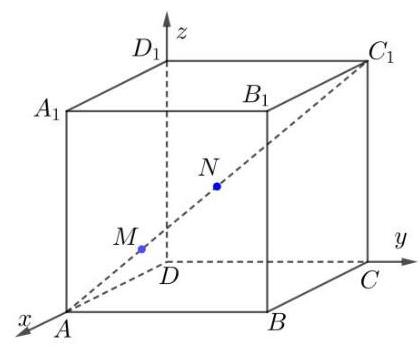
\includegraphics[max width=0.3\textwidth]{images/bo_d7fhnv491nqc73ercsbg_166_1023_759_420_347_0.jpg}
\end{center}
\hspace*{3em} 

【答案】 \(\frac{{32} + 8\sqrt{6}}{3}\)

【解析】依题意,建立空间直角坐标系 \(D - {xyz}\) 如图所示, 则 \(A\left( {4,0,0}\right) ,{C}_{1}\left( {0,4,4}\right)\) ,

因为 \(\overrightarrow{AN} = 2\overrightarrow{AM} = \frac{1}{2}\overrightarrow{A{C}_{1}}\) ，

所以 \(N\left( {2,2,2}\right)\) ， \(M\left( {3,1,1}\right)\) ，设 \(G\left( {x,y,z}\right)\) ，

因为 \(\left| \overrightarrow{GN}\right|  = \sqrt{2}\left| \overrightarrow{GM}\right|\) ,

可得 \(\sqrt{{\left( x - 2\right) }^{2} + {\left( y - 2\right) }^{2} + {\left( z - 2\right) }^{2}} = \sqrt{2} \cdot  \sqrt{{\left( x - 3\right) }^{2} + {\left( y - 1\right) }^{2} + {\left( z - 1\right) }^{2}}\) ,

化简可得 \({\left( x - 4\right) }^{2} + {y}^{2} + {z}^{2} = 6\) ,所以点 \(G\) 在以点 \(A\) 为球心, \(\sqrt{6}\) 为半径的球面上,

则点 \(G\) 到平面 \({A}_{1}{B}_{1}{D}_{1}\) 距离的最大值为 \(4 + \sqrt{6}\) ,

所以 \({\left( {V}_{G - {A}_{1}{B}_{1}{D}_{1}}\right) }_{\max } = \frac{1}{3} \times  \frac{1}{2} \times  {A}_{1}{B}_{1} \cdot  {A}_{1}{C}_{1} \times  \left( {4 + \sqrt{6}}\right)  = \frac{{32} + 8\sqrt{6}}{3}\) .

5.(2025 高三二模奉贤 14)如图，在平行六面体 \({ABCD} - {A}_{1}{B}_{1}{C}_{1}{D}_{1}\) 中，点 \(N\) 在对角线 \({A}_{1}C\) 上,点 \(M\) 在对角线 \({A}_{1}B\) 上, \(\overrightarrow{{A}_{1}N} = \frac{1}{3}\overrightarrow{NC},\overrightarrow{{A}_{1}M} = \frac{1}{2}\overrightarrow{MB}\) ,以下命题正确的是 ( )

\begin{center}
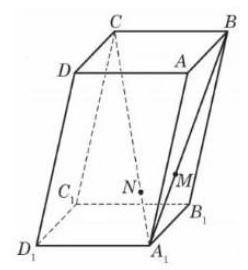
\includegraphics[max width=0.2\textwidth]{images/bo_d7fhnv491nqc73ercsbg_166_1171_1883_248_270_0.jpg}
\end{center}
\hspace*{3em} 

A. \(\overrightarrow{MN}//\overrightarrow{BC}\)

B. \({D}_{1}\text{ 、 }N\text{ 、 }M\) 三点共线

C. \({D}_{1}M\) 与 \({A}_{1}C\) 是异面直线

D. \(\overrightarrow{{D}_{1}N} = \frac{1}{2}\overrightarrow{NM}\)

【答案】B

【解析】

\(\overrightarrow{{D}_{1}M} = \overrightarrow{{D}_{1}{A}_{1}} + \overrightarrow{{A}_{1}M} = \overrightarrow{{D}_{1}{A}_{1}} + \frac{1}{3}\overrightarrow{{A}_{1}B} = \overrightarrow{{D}_{1}{A}_{1}} + \frac{1}{3}\overrightarrow{{A}_{1}{B}_{1}} + \frac{1}{3}\overrightarrow{{B}_{1}B} = \overrightarrow{{D}_{1}{A}_{1}} + \frac{1}{3}\overrightarrow{{D}_{1}{C}_{1}} + \frac{1}{3}\overrightarrow{{D}_{1}D} \; \overrightarrow{{D}_{1}N} = \overrightarrow{{D}_{1}{A}_{1}} + \overrightarrow{{A}_{1}N} = \overrightarrow{{D}_{1}{A}_{1}} + \frac{1}{4}\overrightarrow{{A}_{1}C} = \overrightarrow{{D}_{1}{A}_{1}} + \frac{1}{3}\left( {\overrightarrow{{A}_{1}{B}_{1}} + \overrightarrow{{B}_{1}B} + \overrightarrow{BC}}\right) \; = \frac{3}{4}\overrightarrow{{D}_{1}{A}_{1}} + \frac{1}{4}\overrightarrow{{D}_{1}{C}_{1}} + \frac{1}{4}\overrightarrow{{D}_{1}D} = \frac{3}{4}\overrightarrow{{D}_{1}M}\) ,

故选 B.

6.(2025 高三二模黄浦 14)如图，在平行六面体 \({ABCD} - {A}_{1}{B}_{1}{C}_{1}{D}_{1}\) 中，设 \(\overrightarrow{a} = \overrightarrow{A{A}_{1}}\) ， \(\overrightarrow{b} = \overrightarrow{D{B}_{1}}\) ，若 \(\overrightarrow{a},\overrightarrow{b},\overrightarrow{c}\) 组成空间向量的一个基，则 \(\overrightarrow{c}\) 可以是( )

A. \(\overrightarrow{B{B}_{1}}\) B. \(\overrightarrow{B{C}_{1}}\) C. \(\overrightarrow{BD}\) D. \(\overrightarrow{B{D}_{1}}\)

【答案】B

【解析】A. \(\overrightarrow{B{B}_{1}}\) 与 \(\overrightarrow{A{A}_{1}}\) 平行,故无法构成基向量;

C. 因为 \(\overrightarrow{A{A}_{1}} = \overrightarrow{B{B}_{1}}\) ，可知 \(\overrightarrow{A{A}_{1}}\) ， \(\overrightarrow{BD}\) ， \(\overrightarrow{D{B}_{1}}\) 共面，故无法构成基向量；

D. 同 C，三向量共面，无法构成基向量，故选 B.

7. (2025 高三二模闵行 16) 设 \(n\) 为正整数，空间中 \(n\) 个单位向量构成集合 \({A}_{n} = \left\{  {\overrightarrow{{a}_{1}},\overrightarrow{{a}_{2}},\cdots ,\overrightarrow{{a}_{n}}}\right\}\) ,若存在实数 \(t\) ,满足对任意 \(\overrightarrow{{a}_{i}} \in  {A}_{n},\overrightarrow{{a}_{j}} \in  {A}_{n},\overrightarrow{{a}_{i}} \neq  \overrightarrow{{a}_{j}}\) ,都有 \(\overrightarrow{{a}_{i}} \cdot  \overrightarrow{{a}_{j}} = t\) , 则当 \(n\) 取得最大值时, \(t\) 的值为( ).

A. \(- \frac{1}{2}\) B. \(\frac{1}{2}\) C. \(- \frac{1}{3}\) D. \(\frac{1}{3}\)

【答案】C

【解析】令集合 \({A}_{n} = \left\{  {{\overrightarrow{a}}_{1},{\overrightarrow{a}}_{2},\cdots ,{\overrightarrow{a}}_{n}}\right\}\) 的各向量起点为 \(O\) ,对应终点依次为 \({A}_{1},{A}_{2},\cdots ,{A}_{n}\) , 由向量 \(\overrightarrow{{a}_{i}}\left( {i \in  {\mathrm{N}}^{ * },i \leq  n}\right)\) 为单位向量,则点 \({A}_{1},{A}_{2},\cdots ,{A}_{n}\) 在以 \(O\) 为球心,1 为半径的球面上, 由 \({\overrightarrow{a}}_{i} \in  {A}_{n},{\overrightarrow{a}}_{j} \in  {A}_{n},{\overrightarrow{a}}_{i} \neq  {\overrightarrow{a}}_{j}\) ,得点 \({A}_{1},{A}_{2},\cdots ,{A}_{n}\) 中任意三点不共线,

由 \(t = {\overrightarrow{a}}_{1} \cdot  {\overrightarrow{a}}_{2} = {\overrightarrow{a}}_{2} \cdot  {\overrightarrow{a}}_{3}\) ,得 \(\overrightarrow{O{A}_{2}} \cdot  \left( {\overrightarrow{O{A}_{1}} - \overrightarrow{O{A}_{3}}}\right)  = \overrightarrow{O{A}_{2}} \cdot  \overrightarrow{{A}_{3}{A}_{1}} = 0\) ,则 \(O{A}_{2} \bot  {A}_{1}{A}_{3}\) ,

由 \(t = {\overrightarrow{a}}_{4} \cdot  {\overrightarrow{a}}_{2} = {\overrightarrow{a}}_{2} \cdot  {\overrightarrow{a}}_{3}\) ,同理得 \(O{A}_{2} \bot  {A}_{4}{A}_{3}\) ,而点 \({A}_{1},{A}_{3},{A}_{4}\) 不共线,

于是点 \({A}_{1},{A}_{2},{A}_{3},{A}_{4}\) 不共面,点 \({A}_{1},{A}_{2},{A}_{3},{A}_{4}\) 为球 \(O\) 内接正四面体的 4 个顶点,

若 \(n \geq  5\) ,不妨取 \(n = 5\) ,同理得 \(O{A}_{5} \bot  {A}_{1}{A}_{3},O{A}_{5} \bot  {A}_{4}{A}_{3},O{A}_{5} \bot\) 平面 \({A}_{1}{A}_{3}{A}_{4}\) ,

又 \(O{A}_{5} \bot  {A}_{2}{A}_{3}\) ,由过一点有且只有一个平面垂直于已知直线,得点 \({A}_{2} \in\) 平面 \({A}_{1}{A}_{3}{A}_{4}\) ,

与点 \({A}_{1},{A}_{2},{A}_{3},{A}_{4}\) 不共面矛盾,因此 \({n}_{\max } = 4\) ,设正四面体 \({A}_{1}{A}_{2}{A}_{3}{A}_{4}\) 的棱长为 \(m\) ,

则正 \(\bigtriangleup {A}_{1}{A}_{2}{A}_{3}\) 的外接圆半径为 \(\frac{\sqrt{3}}{2}m \cdot  \frac{2}{3} = \frac{\sqrt{3}}{3}m\) ,正四面体的高为 \(\sqrt{{m}^{2} - {\left( \frac{3}{3}m\right) }^{2}} = \frac{\sqrt{6}}{3}m\) , 球心到平面 \({A}_{1}{A}_{2}{A}_{3}\) 的距离为 \(\frac{\sqrt{6}}{3}m - 1\) ,因此 \({\left( \frac{\sqrt{6}}{3}m - 1\right) }^{2} + {\left( \frac{\sqrt{3}}{3}m\right) }^{2} = {1}^{2}\) ,解得 \(m = \frac{2\sqrt{6}}{3}\) , 所以 \(t = \cos \angle {A}_{1}O{A}_{2} = \frac{{1}^{2} + {1}^{2} - {\left( \frac{2\sqrt{6}}{3}\right) }^{2}}{2 \times  1 \times  1} =  - \frac{1}{3}\) .

故选: C.

8.(2025 高三二模虹口 16)在空间中，点 \(O\) 、 \(A\) 均为定点，且 \(\left| \overrightarrow{OA}\right|  = 1\) . 设集合 \(S = \left\{  {P\left| \right| \overrightarrow{OP}{\left. \right| }^{2} - 2\overrightarrow{OA} \cdot  \overrightarrow{OP} \leq  1}\right\}\) ,则以下说法正确的是 ( ) .

 \circled{1}  若 \(\overrightarrow{OP}\) 在 \(\overrightarrow{OA}\) 上的数量投影为 \(- \frac{1}{5}\) ，则线段 \({OP}\) 在运动过程中所形成的几何体体积为 \(\frac{14}{375}\pi\)

 \circled{2}  对于任意的 \({P}_{i} \in  S\) 以及任意的正实数 \({a}_{i}\) ，设 \(\overrightarrow{OQ} = \mathop{\sum }\limits_{{i = 1}}^{4}{a}_{i}\overrightarrow{O{P}_{i}}\) ，若 \(\mathop{\sum }\limits_{{i = 1}}^{4}{a}_{i} = 1\) ，则 \(Q \in  S\) .

A.  \circled{1} 是真命题， \circled{2} 是真命题 B.  \circled{1} 是真命题， \circled{2} 是假命题

C.  \circled{1} 是假命题， \circled{2} 是真命题 D.  \circled{1} 是假命题， \circled{2} 是假命题

【答案】A

【解析】设 \(\overrightarrow{OA} = \left( {1,0,0}\right) ,P\left( {x,y,z}\right)\) ,

则 \({x}^{2} + {y}^{2} + {z}^{2} - {2x} \leq  1\) ,即 \({\left( x - 1\right) }^{2} + {y}^{2} + {z}^{2} \leq  2\) ,

\(P\) 在以 \(A = \left( {1,0,0}\right)\) 为圆心， \(r = \sqrt{2}\) 的球面及其内部，

对于 \circled{1} ,设点 \(B\) 是点 \(P\) 在 \({OA}\) 上的投影,则由 \(\left| {OP}\right| \cos \left\langle  {\overrightarrow{OP},\overrightarrow{OA}}\right\rangle   =  - \frac{1}{5}\) ,得 \(B\left( {-\frac{1}{5},0,0}\right)\) ,

\({\left| OP\right| }^{2} - 2\left| {OA}\right|  \cdot  \left| {OP}\right| \cos \left\langle  {\overrightarrow{OP},\overrightarrow{OA}}\right\rangle   \leq  1 \Rightarrow  {\left| OP\right| }^{2} \leq  \frac{3}{5},\)

\({\left| BP\right| }^{2} \leq  {\left| OP\right| }^{2} - {\left| OB\right| }^{2} = \frac{3}{5} - \frac{1}{25} = \frac{14}{25},\)

\(P\) 在圆 \(B\) 上及其内部,线段 \({OP}\) 在运动过程中所形成的几何体为圆锥,

\(V = \frac{1}{3}\pi  \cdot  B{P}^{2} \cdot  {OB} = \frac{14}{375}\pi\) , \circled{1} 对;

对于 \circled{2} ， \(\overrightarrow{OQ} = {a}_{1}\overrightarrow{O{P}_{1}} + {a}_{2}\overrightarrow{O{P}_{2}} + {a}_{3}\overrightarrow{O{P}_{3}} + {a}_{4}\overrightarrow{O{P}_{4}}\) ，

\({a}_{1} + {a}_{2} + {a}_{3} + {a}_{4} = 1,\overrightarrow{OQ} = {a}_{1}\overrightarrow{O{P}_{1}} + {a}_{2}\overrightarrow{O{P}_{2}} + {a}_{3}\overrightarrow{O{P}_{3}} + \left( {1 - {a}_{1} - {a}_{2} - {a}_{3}}\right) \overrightarrow{O{P}_{4}}\) ,

\(\overrightarrow{{P}_{4}Q} = {a}_{1}\overrightarrow{{P}_{4}{P}_{1}} + {a}_{2}\overrightarrow{{P}_{4}{P}_{2}} + {a}_{3}\overrightarrow{{P}_{4}{P}_{3}}\) ,由于 \({a}_{1} + {a}_{2} + {a}_{3} + {a}_{4} = 1,{a}_{1},{a}_{2},{a}_{3},{a}_{4} > 0\) ,

所以 \(0 < {a}_{1},{a}_{2},{a}_{3} < 1,{a}_{1} + {a}_{2} + {a}_{3} < 1\) ,所以点 \(Q\) 在四面体 \({P}_{1}{P}_{2}{P}_{3}{P}_{4}\) 上,

又由于 \(P\) 在球面及球内部, \(\therefore Q \in  S\) , \circled{2} 对;

故选 A.

\section*{第八部分 计数原理、概率、统计}

\section*{一、排列与组合}

1. (2025 高三二模松江 7)有 4 辆车停放在 5 个并排车位上，客车甲车体较宽，停放时需要占两个车位，并且乙车与客车甲相邻停放，则共有\_\_\_\_\_种不同的停放方法.

【答案】 12

【解析】客车甲与乙相邻, 甲车占两个车位, 将这两个车位看作一个整体, 相当于有 4 个车位,同时将甲乙看作一个整体,相当于有 3 两车,甲乙内部排序 \({P}_{2}^{2}\) ,三个车位排序 \({P}_{3}^{3}\) ,因此共有 \({P}_{2}^{2}{P}_{3}^{3} = {12}\) 种停车方法.

2.(2025 高三二模宝山 10)有 3 件商品的编号分别为 \(i\left( {i = 1,2,3}\right)\) ，它们的售价(元) \(S\left( i\right)  \in  \{ 5,7,8,{10},{11},{20}\}\) ,且满足 \(S\left( 1\right)  \leq  S\left( 2\right)  \leq  S\left( 3\right)\) ,则这 3 件商品售价的所有可能情况有\_\_\_\_\_种.

【答案】56

【解析】 \({1}^{ \circ  }\) 当 3 件商品售价均不相同,共有 \({C}_{6}^{3} = {20}\) 种情况,

\({2}^{ \circ  }\) 当 3 件商品有两件商品售价相同则有 \(S\left( 1\right)  = S\left( 2\right)  < S\left( 3\right)\) 或 \(S\left( 1\right)  < S\left( 2\right)  = S\left( 3\right)\) 两类情况,共有 \(2 \times  {C}_{6}^{2} = {30}\) 种情况;

\({3}^{ \circ  }\) 当 3 件商品的售价均相同,共有 6 种情况;

综上,共有 \({20} + {30} + 6 = {56}\) 种情况.

3.(2025 高三二模虹口 10)已知 9 个小球的编号为 1、2、...、9，从中有放回地摸取小球三次，并依次记录其编号，若这三个编号按此顺序成等差数列，则共有\_\_\_\_\_种不同的摸取方法.

【答案】 41

【解析】只要第一次和第三次同时为奇数和偶数, 若为等差数列, 则第二次的数字就相对确定了,则不同的摸取方法是 \(5 \times  5 + 4 \times  4 = {41}\) .

4. (2025 高三二模普陀 10)设 \(i,j,n\) 为正整数，集合 \(M = \{ 1,3,5,\cdots ,{2n} - 1\}\) ，若集合 \(A\) 满足 \(A \subseteq  M\) ,且对 \(A\) 中任意的两个元素 \(i,j\) 皆有 \(\left| {i - j}\right|  > 4\) 成立,记满足条件的集合 \(A\) 的个数为 \({a}_{n}\) ,则 \({a}_{8} =\) \_\_\_\_\_.

【答案】 19

【解析】由题意,当 \(n = 8\) 时, \(M = \{ 1,3,5,7,9,{11},{13},{15}\}\) ,由题意, \(A\) 至少 2 个元素,至多 3 个元素,若 \(A\) 中有 2 个元素,根据隔板法,可知由 \({C}_{6}^{2} = {15}\) 种情况 (也可枚举);

若 \(A\) 中有 3 个元素,有 \({C}_{4}^{1} = 4\) 种情况;

因此共有 \({15} + 4 = {19}\) 种情况.

5.(2025 高三二模静安 11)从 \(m\) 个男生和 \(n\) 个女生(10≥m>n≥4)中任选 2 个人当队长,假设事件 \(A\) 表示选出的 2 人性别相同,事件 \(B\) 表示选出的 2 人性别不同. 如果事件 \(A\) 的概率和事件 \(B\) 的概率相等,那么 \(m - n\) 的可能值为\_\_\_\_\_.

【答案】 4

【解析】由题意得 \(\frac{{C}_{m}^{2} + {C}_{n}^{2}}{{C}_{m + n}^{2}} = \frac{{C}_{m}^{1}{C}_{n}^{1}}{{C}_{m + n}^{2}} \Rightarrow  \frac{m\left( {m - 1}\right) }{2} + \frac{n\left( {n - 1}\right) }{2} = {mn}\) ,

\(\therefore {m}^{2} + {n}^{2} = m + n + {2mn}\) ,整理得, \({\left( m - n\right) }^{2} = m + n\)

由 \(9 \leq  m + n \leq  {19}\) ,得 \(m + n = 9\) (舍) 或 \(m + n = {16}\) ,

故 \(m - n = 4\) .

6.(2025 高三二模奉贤 13)下列有关排列组合数的计算公式，错误的是( )

A. \({P}_{n}^{m} + {P}_{n}^{m - 1} = {P}_{n + 1}^{m}\left( {m,n}\right.\) 是正整数,且 \(m \leq  n)\)

B. \({P}_{n}^{m} = {C}_{n}^{m}{P}_{m}^{m}\left( {m,n\text{ 是正整数,且 }m \leq  n}\right)\)

C. \({P}_{n}^{m} = n{P}_{n - 1}^{m - 1}\left( {m,n\text{ 是正整数,且 }m \leq  n}\right)\)

D. \({C}_{n}^{m} + {C}_{n}^{m - 1} = {C}_{n + 1}^{m}\left( {m,n}\right.\) 是正整数,且 \(\left. {m \leq  n}\right)\)

【答案】A

【解析】对于 \(\mathrm{A},{P}_{n}^{m} + {P}_{n}^{m - 1} = \frac{n!}{\left( {n - m}\right) !} + \frac{n!}{\left( {n - m + 1}\right) !} = \frac{\left( {n - m + 1 + 1}\right) n!}{\left( {n - m + 1}\right) !} = \frac{\left( {n - m + 2}\right) n!}{\left( {n - m + 1}\right) !} \; {P}_{n + 1}^{m} = \frac{\left( {n + 1}\right) !}{\left( {n + 1 - m}\right) !} \neq  \frac{\left( {n - m + 2}\right) n!}{\left( {n - m + 1}\right) !}\) ,故选 A.

7.(2025 高三二模杨浦 14)3 名同学报名参加社团活动，有 4 个社团可以报名，这些社团招收人数不限，但每位同学只能报名其中 1 个社团，则这 3 位同学可能的报名结果共有( ) 种

A. 6 B. 24 C. 64 D. 81

【答案】C

【解析】每个学生有 4 种选择,故有 \({4}^{3} = {64}\) 种选择.

\section*{二、二项式定理}

1.(2025 高三二模青浦 3)(1-ax) \({}^{6}\) 的二项展开式中 \({x}^{3}\) 项的系数是 20，则实数 \(a\) 的值是\_\_\_\_\_.

【答案】 \(a =  - 1\)

【解析】设 \({T}_{r + 1} = {C}_{6}^{r}{\left( -ax\right) }^{r}\) 为含 \({x}^{3}\) 的项,则 \(r = 3\) ,则 \({C}_{6}^{3}{\left( -a\right) }^{3} = {20} \Rightarrow  a =  - 1\) .

2.(2025 高三二模奉贤 4)在( \(\sqrt{x} - \frac{2}{x}{)}^{9}\) 的二项展开式中，常数项为\_\_\_\_\_.(用数字作答)

【答案】-672

【解析】设 \({T}_{r + 1} = {C}_{9}^{r}{\left( \sqrt{x}\right) }^{9 - r}{\left( -2{x}^{-1}\right) }^{r} = {C}_{9}^{r}{\left( -2\right) }^{r}{x}^{\frac{9}{2} - \frac{3}{2}r}\) 为常数项，则 \(\frac{9}{2} - \frac{3}{2}r = 0,r = 3\) 则 \({C}_{9}^{3}{\left( -2\right) }^{3} =  - {672}\) .

3.(2025 高三二模松江 5) \({\left( 3{x}^{2} + \frac{1}{x}\right) }^{6}\) 的二项展开式中的常数项为\_\_\_\_\_.

【答案】 135

【解析】 \({T}_{r + 1} = {C}_{6}^{r}{\left( 3{x}^{2}\right) }^{6 - r}{\left( {x}^{-1}\right) }^{r} = {C}_{6}^{r} \cdot  {3}^{6 - r} \cdot  {x}^{{12} - {3r}},{12} - {3r} = 0\) 解得 \(r = 4\) , 所以常数项为 \({C}_{6}^{4} \cdot  {3}^{6 - 4} = {135}\) .

4.(2025 高三二模闵行 5)在( \({2x} + \frac{1}{x}{)}^{6}\) 的二项展开式中，常数项是\_\_\_\_\_.(用数值作答)

【答案】 160

【解析】假设 \({T}_{r + 1} = {C}_{6}^{r}{\left( 2x\right) }^{6 - r}{\left( {x}^{-1}\right) }^{r} = {C}_{6}^{r}{2}^{6 - r}{x}^{6 - {2r}}\) 为常数项,则 \(6 - {2r} = 0 \Rightarrow  r = 3\) , 则常数项为 \({T}_{4} = {C}_{6}^{3}{2}^{3} = {160}\) .

5.(2025 高三二模金山 5)在( \({ax} + \frac{1}{x}{)}^{5}\) 展开式中 \(x\) 的系数为 80，则实数 \(a\) 的值为\_\_\_\_\_.

【答案】 2

【解析】假设 \({T}_{r + 1} = {C}_{5}^{r}{\left( ax\right) }^{5 - r}{\left( {x}^{-1}\right) }^{r} = {C}_{5}^{r}{2}^{5 - r}{x}^{5 - {2r}}\) 为含的 \(x\) 项,则 \(5 - {2r} = 1 \Rightarrow  r = 2\) ,则 \({C}_{5}^{2}{a}^{3} = {80} \Rightarrow  a = 2.\)

6.(2025 高三二模嘉定 5)在( \({2x} - \frac{1}{\sqrt{x}}{)}^{6}\) 的二项展开式中，常数项的值为\_\_\_\_\_.

【答案】 60

【解析】 \({T}_{r + 1} = {C}_{6}^{r}{\left( 2x\right) }^{6 - r}{\left( -{x}^{-\frac{1}{2}}\right) }^{r} = {\left( -1\right) }^{r} \cdot  {2}^{6 - r} \cdot  {C}_{6}^{r} \cdot  {x}^{6 - \frac{3}{2}r},6 - \frac{3}{2}r = 0 \Rightarrow  r = 4\) , 所以常数项的值为 \({\left( -1\right) }^{4} \cdot  {2}^{2} \cdot  {C}_{6}^{4} = {60}\) .

7.(2025 高三二模杨浦 6)在 \({\left( x + \frac{1}{\sqrt{x}}\right) }^{6}\) 的二项展开式中，常数项的值为\_\_\_\_\_.

【答案】 15

【解析】 \({T}_{r + 1} = {C}_{6}^{r} \cdot  {x}^{6 - r} \cdot  {\left( {x}^{-\frac{1}{2}}\right) }^{r} = {C}_{6}^{r} \cdot  {x}^{6 - \frac{3}{2}r}\) ,则 \(6 - \frac{3}{2}r = 0 \Rightarrow  r = 4\) ,所以常数项为 \({C}_{6}^{4} = {15}\) .

8.(2025 高三二模宝山 6) \({\left( x + \frac{2}{x}\right) }^{6}\) 的二项展开式中， \({x}^{2}\) 项的系数为\_\_\_\_\_.

【答案】60

【解析】 \({T}_{r + 1} = {C}_{6}^{r} \cdot  {x}^{6 - r} \cdot  {\left( 2{x}^{-1}\right) }^{r} = {C}_{6}^{r} \cdot  {2}^{r} \cdot  {x}^{6 - {2r}},6 - {2r} = 2 \Rightarrow  r = 2\) ,所以 \({x}^{2}\) 项的系数为 \({C}_{6}^{2} \cdot  {2}^{2} = {60}\) .

9.(2025 高三二模普陀 6)设 \(t \in  \mathbf{R}\) ，若 \(\left( {1 + \frac{t}{x}}\right) {\left( 1 - x\right) }^{6}\) 的展开式中 \({x}^{3}\) 项的系数为 10，则 \(t =\)

【答案】 2

【解析】由题意, \({10}{x}^{3} = 1 \cdot  {C}_{6}^{3} \cdot  {1}^{3} \cdot  {\left( -x\right) }^{3} + \frac{t}{x} \cdot  {C}_{6}^{4} \cdot  {1}^{2} \cdot  {\left( -x\right) }^{4} =  - {20}{x}^{3} + {15t}{x}^{3}\) ,解得 \(t = 2\) . 10.(2025 高三二模浦东 7) \({\left( x - \frac{1}{x}\right) }^{10}\) 的二项展开式中常数项为\_\_\_\_\_.

【答案】-252

【解析】 \({T}_{r + 1} = {C}_{10}^{r} \cdot  {x}^{{10} - r} \cdot  {\left( -{x}^{-1}\right) }^{r} = {\left( -1\right) }^{r} \cdot  {C}_{10}^{r} \cdot  {x}^{{10} - {2r}}\) ,当 \({10} - {2r} = 0\) 时, \(r = 5\) , 则常数项为 \({\left( -1\right) }^{5} \cdot  {C}_{10}^{5} =  - {252}\) .

11. (2025 高三二模崇明 9)已知 \({\left( x + 1\right) }^{10} = {a}_{0} + {a}_{1}\left( {x - 1}\right)  + {a}_{2}{\left( x - 1\right) }^{2} + \cdots  + {a}_{10}{\left( x - 1\right) }^{10}\) ，则 \({a}_{0} + {a}_{1} + {a}_{2} + \cdots  + {a}_{10} =\) \_\_\_\_\_.

【答案】 \({3}^{10}\)

【解析】令 \(x = 2\) ,则 \({a}_{0} + {a}_{1} + {a}_{2} + \cdots  + {a}_{10} = {3}^{10}\) .

\section*{三、概率}

1.(2025 高三二模奉贤 3)假设生产某产品的一个部件来自三个供应商，供货占比分别是 \(\frac{1}{2}\) 、 \(\frac{1}{6}\text{ 、 }\frac{1}{3}\) ，而它们的良品率分别是 \({0.96}\text{ 、 }{0.90}\text{ 、 }{0.93}\) ，则该部件的总体良品率是\_\_\_\_\_.

【答案】0.94

【解析】该部件的总体良品率为 \(\frac{1}{2} \times  {0.96} + \frac{1}{6} \times  {0.90} + \frac{1}{3} \times  {0.93} = {0.94}\) .

2.(2025 高三二模普陀 3)已知事件 \(A\) 与事件 \(B\) 相互独立，若 \(P\left( {A \cap  \bar{B}}\right)  = \frac{3}{25},P\left( B\right)  = \frac{3}{5}\) ， 则 \(P\left( A\right)  =\) \_\_\_\_\_.

【答案】 \(\frac{3}{10}\)

【解析】因为 \(P\left( B\right)  = \frac{3}{5}\) ,所以 \(P\left( \bar{B}\right)  = \frac{2}{5}\) ,因为事件 \(A\) 与事件 \(B\) 相互独立,则事件 \(A\) 与事件 \(\bar{B}\) 相互独立,所以 \(P\left( {A \cap  \bar{B}}\right)  = P\left( A\right) P\left( \bar{B}\right)  = \frac{3}{25}\) ,解得 \(P\left( A\right)  = \frac{3}{10}\) .

3.(2025 高三二模静安 4)已知随机变量 \(X\) 服从二项分布 \(B\left( {n,p}\right)\) ，若 \(E\left\lbrack  X\right\rbrack   = {30}\) ， \(D\left\lbrack  X\right\rbrack   = {20}\) ， 则 \(p\) 的值为\_\_\_\_\_.

【答案】 \(\frac{1}{3}\)

【解析】由题意知 \(\left\{  {\begin{array}{l} {np} = {30} \\  {np}\left( {1 - p}\right)  = {20} \end{array} \Rightarrow  1 - p = \frac{2}{3} \Rightarrow  p = \frac{1}{3}}\right.\) .

4. (2025 高三二模长宁 4)某水果店的苹果，60\%来自 A 基地，40\%来自 B 基地，A 基地苹果的新鲜率为 90\%，B 基地苹果的新鲜率为 85\%，从该水果店随机选取一个苹果，则选到新鲜苹果的概率是\_\_\_\_\_.

【答案】 \({88}\% \left( {{0.88}\text{ 或 }\frac{22}{25}}\right)\)

【解析】由全概公式可得 \(P = {60}\%  \times  {90}\%  + {40}\%  \times  {85}\%  = {88}\%\) .

5.(2025 高三二模长宁 6)已知随机变量 \(X\) 的分布是 \(\left( \begin{matrix}  - 1 & 0 & 1 \\  \frac{1}{4} & \frac{1}{4} & \frac{1}{2} \end{matrix}\right)\) ，则其方差 \(D\left\lbrack  X\right\rbrack   =\) \_\_\_\_\_.

【答案】 \(\frac{11}{16}\)

【解析】 \(E\left\lbrack  X\right\rbrack   =  - 1 \times  \frac{1}{4} + 0 \times  \frac{1}{4} + 1 \times  \frac{1}{2} = \frac{1}{4}\) ,

\(D\left\lbrack  X\right\rbrack   = E\left\lbrack  {X}^{2}\right\rbrack   - {E}^{2}\left\lbrack  X\right\rbrack   = {\left( -1\right) }^{2} \times  \frac{1}{4} + {0}^{2} \times  \frac{1}{4} + {1}^{2} \times  \frac{1}{2} - {\left( \frac{1}{4}\right) }^{2} = \frac{11}{16}.\)

6.(2025 高三二模静安 7)设一个罐子中有大小与质地相同的黑、白、红三个球，不放回的每次摸一个球,设第一次没有摸到黑球是事件 \(A\) ,第二次没有摸到黑球是事件 \(B\) ,则 \(P\left( {B \mid  A}\right)\) 的值为\_\_\_\_\_.

【答案】 \(\frac{1}{2}\)

【解析】 \(P\left( {B \mid  A}\right)  = \frac{P\left( {AB}\right) }{P\left( A\right) } = \frac{\frac{2}{3} \times  \frac{1}{2}}{\frac{2}{3}} = \frac{1}{2}\) .

7.(2025 高三二模普陀)在一个不透明的盒中装着标有数字 1,2,3,4 的大小与质地都相同的小球各 2 个,现从该盒中一次取出 2 个球,设事件 \(A\) 为“取出 2 个球的数字之和大于 5 ”,事件 \(B\) 为“取出的 2 个球中最小数字是 2 ”，则 \(P\left( {B \mid  A}\right)  =\) \_\_\_\_\_.

【答案】 \(\frac{2}{5}\)

【解析】由题意, 盒中共有 8 个小球, 2 个球数字之和大于 5 的组合有“2,4”“3,3”“3,4”“4,4”, 所以 \(P\left( A\right)  = \frac{{C}_{2}^{1} \cdot  {C}_{2}^{1} + {C}_{2}^{2} + {C}_{2}^{1} \cdot  {C}_{2}^{1} + {C}_{2}^{2}}{{C}_{8}^{2}} = \frac{5}{14},P\left( {AB}\right)  = \frac{{C}_{2}^{1} \cdot  {C}_{2}^{1}}{{C}_{8}^{2}} = \frac{1}{7}\) ,

则 \(P\left( {B \mid  A}\right)  = \frac{P\left( {AB}\right) }{P\left( A\right) } = \frac{\frac{1}{7}}{\frac{5}{14}} = \frac{2}{5}\) .

8.(2025 高三二模青浦 8)已知随机变量 \(\xi  \sim  N\left( {3,{\sigma }^{2}}\right) \left( {\sigma  > 0}\right)\) ，若 \(P\left( {\xi  \geq  1}\right)  = {0.9}\) ，则 \(P\left( {3 \leq  \xi  \leq  5}\right)  =\) \_\_\_\_\_.

【答案】0.4

【解析】 \(\because P\left( {\xi  \geq  5}\right)  = P\left( {\xi  \leq  1}\right)  = 1 - P\left( {\xi  \geq  1}\right)  = 1 - {0.9} = {0.1}\) ,

\(\therefore P\left( {3 \leq  \xi  \leq  5}\right)  = {0.5} - {0.1} = {0.4}\) .

9.(2025 高三二模徐汇 9)已知两个随机事件 \(A,B\) ，若 \(P\left( A\right)  = \frac{1}{5},P\left( B\right)  = \frac{1}{4},P\left( {B \mid  A}\right)  = \frac{2}{3}\) ， 则 \(P\left( {\bar{A} \mid  B}\right)  =\) \_\_\_\_\_.

【答案】 \(\frac{7}{15}\)

【解析】 \(\because P\left( {B \mid  A}\right)  = \frac{P\left( {AB}\right) }{P\left( A\right) } = \frac{P\left( {AB}\right) }{\frac{1}{5}} = \frac{2}{3},\therefore P\left( {AB}\right)  = \frac{2}{15}\) ,

\(\therefore P\left( {\bar{A}B}\right)  = P\left( B\right)  - P\left( {AB}\right)  = \frac{1}{4} - \frac{2}{15} = \frac{7}{60},\therefore P\left( {\bar{A} \mid  B}\right)  = \frac{P\left( {\bar{A}B}\right) }{P\left( B\right) } = \frac{\frac{7}{60}}{\frac{1}{4}} = \frac{7}{15}\) .

10.(2025 高三二模金山 9)体育课上需要进行投篮测试，规定每人投 3 次，至少投中 2 次才能通过测试. 已知某同学每次投篮投中的概率均为 0.6 ，且各次投篮是否投中相互独立， 则该同学通过测试的概率为\_\_\_\_\_.

【答案】 \(\frac{81}{125}\)

【解析】该同学通过测试的概率为 \({C}_{3}^{2} \times  {\left( {0.6}\right) }^{2} \times  \left( {1 - {0.6}}\right)  + {C}_{3}^{3} \times  {\left( {0.6}\right) }^{3} = \frac{81}{125}\) .

11.(2025 高三二模嘉定 9)在由 \(1\text{ 、 }2\text{ 、 }3\text{ 、 }4\text{ 、 }5\) 这五个数组成的无重复数字的四位数中， 其能被 3 整除的概率为\_\_\_\_\_.

【答案】 \(\frac{1}{5}\)

【解析】只有 \(1\text{ 、 }2\text{ 、 }4\text{ 、 }5\) 这四个数组成的四位数可以被 3 整除,所以 \(P = \frac{{P}_{4}^{4}}{{P}_{5}^{4}} = \frac{1}{5}\) .

12.(2025 高三二模虹口)某工厂生产的零件长度 \(X\) (单位:毫米)服从正态分布 \(N\left( {3,{\sigma }^{2}}\right)\) ， 且 \(P\left( {\left| {X - 3}\right|  \leq  {0.5}}\right)  = {0.8}\) ，若对该工厂同批生产的 4 个零件逐一检查，则仅有1 个零件的长度大于 3.5 毫米的概率为\_\_\_\_\_.

【答案】0.2916

【解析】 \(\because P\left( {\left| {X - 3}\right|  \leq  {0.5}}\right)  = P\left( {{2.5} \leq  X \leq  {3.5}}\right)  = {0.8},\therefore P\left( {X > {3.5}}\right)  = \frac{1 - {0.8}}{2} = {0.1}\) , 则仅有一个零件的长度大于 3.5 毫米的概率为 \({C}_{4}^{1} \times  {0.1} \times  {0.9}^{3} = {0.2916}\) .

13.(2025 高三二模闵行 9)某公司生产的糖果每包的标识质量是 500 克，但公司承认实际质量存在误差. 已知每包糖果的实际质量服从正态分布 \(N\left( {{500},{\sigma }^{2}}\right)\) ,且任意一包的糖果质量介于 495 克到 505 克之间的可能性为 95.4\%，则随意买一包该公司生产的糖果，其质量超过 505 克的可能性约为\_\_\_\_\_. (精确到 0.1\%)

【答案】 2.3\%

【解析】由题意可知 \({\sigma }^{2} = {2.5}^{2}\) ,则质量超过 505 的可能性为 \(\frac{1 - {95.4}\% }{2} = {2.3}\%\) .

14.(2025 高三二模长宁 9)一项过关游戏的规则规定:在第 \(n\) 关要投掷骰子 \(n\) 次，如果这 \(n\) 次投掷所得的点数之和大于 \({3n}\) ，则算过关，问一个人连过第一、二关的概率为\_\_\_\_\_.

【答案】 \(\frac{7}{24}\)

【解析】第一关要投掷 1 次骰子,且点数要大于 3,概率 \({p}_{1} = \frac{1}{2}\) ,第二关要投掷 2 次骰子, 点数之和要大于 6,投掷点数小于等于 6 的情况有 \(\left( {1,1}\right) ,\left( {1,2}\right) ,\left( {1,3}\right) ,\left( {1,4}\right) ,\left( {1,5}\right)\) , \(\left( {2,1}\right) ,\left( {2,2}\right) ,\left( {2,3}\right) ,\left( {2,4}\right) ,\left( {3,1}\right) ,\left( {3,2}\right) ,\left( {3,3}\right) ,\left( {4,1}\right) ,\left( {4,2}\right) ,\left( {5,1}\right)\) 共 15 种情况,所以 \({p}_{2} = 1 - \frac{15}{36} = \frac{7}{12}\) ,所以连过一二关的概率 \(P = {p}_{1}{p}_{2} = \frac{7}{24}\) .

15.(2025 高三二模嘉定 10)已知某次数学的测试成绩 \(X\) 服从 \(\mu  = {75}\text{ 、 }{\sigma }^{2} = {64}\) 的正态分布, 若小明的成绩不低于 91 分那么他的成绩大约超过了\_\_\_\_\_ \(\%\) 的学生. (精确到 0.1\%) (参考数据: \(P\left( {\left| X\right|  < \sigma }\right)  \approx  {68.3}\% ,P\left( {\left| X\right|  < {2\sigma }}\right)  \approx  {95.4}\% ,P\left( {\left| X\right|  < {3\sigma }}\right)  \approx  {99.7}\%\) )

【答案】97.7

【解析】令自变量 \(Y = \frac{X - \mu }{\sigma }\) ,则 \(Y \sim  N\left( {0,1}\right) ,\frac{{91} - {75}}{8} = 2\) ,

所以 \(P\left( {X > {91}}\right)  = P\left( {Y > 2}\right)  = \frac{1 - P\left( {\left| Y\right|  < 2}\right) }{2} \approx  {2.3}\%\) .

所以小明超过了大约 1-2.3\% = 97.7\% 的学生.

16.(2025 高三二模奉贤 10)盒子中有大小与质地均相同的 \(a\) 个红球和 \(b\) 个白球，从中随机取 1 个球,观察其颜色后放回,并同时放入与其相同颜色的球 \(c\) 个(大小与质地均相同), 再从中随机取 1 个球，计算此次取到白球的概率是\_\_\_\_\_.

【答案】 \(\frac{b}{a + b}\)

【解析】由题意知取到白球的概率是

\(\frac{a}{a + b} \times  \frac{b}{a + b + c} + \frac{b}{a + b} \times  \frac{b + c}{a + b + c} = \frac{b\left( {a + b + c}\right) }{\left( {a + b}\right) \left( {a + b + c}\right) } = \frac{b}{a + b}.\)

17.(2025 高三二模黄浦 10)若从 2025 的所有正约数中任取一个数，则这个数是一个完全平方数的概率为\_\_\_\_\_.

【答案】 \(\frac{2}{5}\)

【解析】2025 \(= {3}^{4} \times  {5}^{2}\) ,其正约数共有 \(5 \times  3 = {15}\) 个,

其中为完全平方数的有 \(1\text{ 、 }{3}^{2}\text{ 、 }{3}^{4}\text{ 、 }{5}^{2}\text{ 、 }{3}^{2} \times  {5}^{2},{3}^{4} \times  {5}^{2}\) ,共 6 个,

所以 \(P = \frac{6}{15} = \frac{2}{5}\) .

18.(2025 高三二模徐汇 13)已知两个随机事件 \(A,B\) ，则“ \(A\) 与 \(B\) 互斥”是“ \(A\) 与 \(B\) 对立”的 ( )

A. 充分非必要条件 B. 必要非充分条件 C. 充要条件 D. 既非充分也非必要条件

【答案】B

【解析】对立可以推出互斥, 互斥推不出对立, 故选 B.

19.(2025 高三二模虹口 15)春节期间，小明和弟弟玩起了一种自定义游戏，规定先由弟弟掷一颗质量均匀的骰子, 若弟弟掷出的点数为 6 , 则吃 1 颗花生; 若掷出其他点数, 则记下这个点数, 然后由小明开始两个人轮流掷这颗骰子, 直至任意一方掷出这个记下的点数或者 6，一次游戏结束.若掷出的是这个记下的点数，则弟弟吃 1 颗花生；若是 6，则小明吃 3 颗花生.任意一次游戏中弟弟能吃到 1 颗花生的概率为( ).

A. \(\frac{5}{24}\) B. \(\frac{5}{12}\) C. \(\frac{3}{8}\) D. \(\frac{7}{12}\)

【答案】D

【解析】记 \({P}_{n}\) 为一次游戏中弟弟第 \(n\) 轮吃到一颗花生的概率, \({P}_{n} = \frac{1}{6}\) ,

\(P\) 为一次游戏中弟弟吃到一颗花生的概率,

则 \(P = {P}_{1} + \frac{5}{6}{P}_{2} + \frac{5}{6} \times  \frac{2}{3} \times  {P}_{3} + \frac{5}{6} \times  {\left( \frac{2}{3}\right) }^{2} \times  {P}_{4} + \cdots  + \frac{5}{6} \times  {\left( \frac{2}{3}\right) }^{n - 2} \times  {P}_{n} + \cdots\)

\(= \frac{1}{6} + \frac{5}{36} + \frac{5}{36} \times  \frac{2}{3} \times  {P}_{3} + \frac{5}{36} \times  {\left( \frac{2}{3}\right) }^{2} + \cdots  + \frac{5}{36} \times  {\left( \frac{2}{3}\right) }^{n - 2} + \cdots\)

\(= \frac{1}{6} + \frac{\frac{5}{36}}{1 - \frac{2}{3}} = \frac{7}{12}\) ,

故选 D.

20. ( 2025 高三二模青浦 15 )一个质地均匀的正四面体，四个面上分别标有数字1,2,3,4. 任意掷一次该四面体，观察它与地面接触面上的数字，得到样本空间 \(\Omega  = \{ 1,2,3,4\}\) ，记事件 \(A = \{ 1,2\}\) ,事件 \(B = \{ 1,3\}\) ,事件 \(C = \{ 1,4\}\) ,则(   ).

A. 事件 \(A,B,C\) 两两独立,事件 \(A,B,C\) 相互独立

B. 事件 \(A,B,C\) 两两独立,事件 \(A,B,C\) 不相互独立

C. 事件 \(A,B,C\) 不两两独立,事件 \(A,B,C\) 相互独立

D. 事件 \(A,B,C\) 不两两独立,事件 \(A,B,C\) 不相互独立

【答案】B

【解析】由题意知

\(P\left( A\right)  = \frac{1}{2},P\left( B\right)  = \frac{1}{2},P\left( C\right)  = \frac{1}{2},P\left( {A \cap  B}\right)  = \frac{1}{4},P\left( {A \cap  C}\right)  = \frac{1}{4},P\left( {B \cap  C}\right)  = \frac{1}{4},P\left( {A \cap  B \cap  C}\right)  = \frac{1}{4}\)

\(\therefore P\left( {A \cap  B}\right)  = P\left( A\right) P\left( B\right) ,P\left( {AC}\right)  = P\left( A\right) P\left( C\right) ,P\left( {B \cap  C}\right)  = P\left( B\right) P\left( C\right)\) ,

但是 \(P\left( {A \cap  B \cap  C}\right)  \neq  P\left( A\right) P\left( B\right) P\left( C\right)\) ,故选 B.

21. (2025 高三二模徐汇 15)在桌面上有一个质地均匀的正四面体 \(D - {ABC}\) . 从该正四面体与桌面贴合的面上的三条棱中等可能地选取一条棱, 沿其翻转正四面体至正四面体的另一个面与桌面贴合, 如此翻转称为一次操作. 如图, 开始时,正四面体与桌面贴合的面为 \({ABC}\) ,操作 \(n\left( {n = 1,2,3,\cdots }\right)\) 次后,正四面体与桌面贴合的面是 \({ABC}\) 的概率记为 \({P}_{n}\) .

\begin{center}
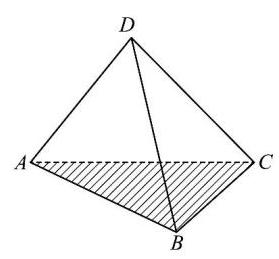
\includegraphics[max width=0.2\textwidth]{images/bo_d7fhnv491nqc73ercsbg_178_1246_1703_279_259_0.jpg}
\end{center}
\hspace*{3em} 

现有下列两个结论:  \circled{1}  \({P}_{2} = \frac{1}{3}\) ;  \circled{2}  \({P}_{25} < {P}_{24}\) .

则下列说法正确的是( )

A.  \circled{1} 正确， \circled{2} 错误 B.  \circled{1} 错误， \circled{2} 正确

C.  \circled{1} 、 \circled{2} 都错误 D.  \circled{1} 、 \circled{2} 都错误

【答案】C

【解析】 \circled{1} ,假设第一次沿着棱 \({AB}\) 翻转,此时面 \({ABD}\) 与桌面贴合,若再翻转 1 次,可能与桌面贴合的面的情况有 \({ABC},{BCD},{ACD}\) ,则 \({P}_{1} = 0,{P}_{2} = \frac{1}{3}\) , \circled{1} 正确;

 \circled{2} 若操作 \(n\) 次后，正四面题与桌面贴合的面是 \({ABC}\) 的概率为 \({P}_{n}\) ，则操作 \(n - 1\) 次后，正四面题与桌面贴合的面是 \({ABC}\) 的概率为 \({P}_{n - 1}\) ,则操作 \(n - 2\) 次后,正四面题与桌面贴合的面是 \({ABC}\) 的概率为 \({P}_{n - 2}\) ,

则 \({P}_{n} = \frac{1}{3}\left( {1 - {P}_{n - 1}}\right)  \Rightarrow  {P}_{n} - \frac{1}{4} =  - \frac{1}{3}\left( {{P}_{n - 1} - \frac{1}{4}}\right)  \Rightarrow  {P}_{n} - \frac{1}{4} =  - \frac{1}{4} \cdot  {\left( -\frac{1}{3}\right) }^{n - 1}\) ,

\(\therefore {P}_{n} = \frac{1}{4} + \frac{1}{12} \cdot  {\left( -\frac{1}{3}\right) }^{n - 2}\left( {n \geq  3}\right) ,{P}_{\text{ 奇 }} < {P}_{\text{ 偶 }}\) ,

 \circled{2} 正确；故选 C.

22.(2025 高三二模崇明 15)抛掷一枚质地均匀的硬币 \(n\) 次(其中 \(n\) 为大于等于 2 的整数)， 设事件 \(A\) 表示 “ \(n\) 次中既有正面朝上又有反面朝上”，事件 \(B\) 表示 “ \(n\) 次中至多有一次正面朝上”,若事件 \(A\) 与事件 \(B\) 是独立的,则 \(n\) 的值为( )

A. 5 B. 4 C. 3 D. 2

【答案】C

【解析】由题意知 \(P\left( A\right)  = 1 - \frac{2}{{2}^{n}},P\left( B\right)  = \frac{1 + n}{{2}^{n}},P\left( {A \cap  B}\right)  = \frac{n}{{2}^{n}}\) ,

因为事件 \(A\) 和事件 \(B\) 相互独立，

则 \(P\left( A\right)  \cdot  P\left( B\right)  = P\left( {A \cap  B}\right)  \Rightarrow  \left( {1 - \frac{2}{{2}^{n}}}\right)  \cdot  \frac{1 + n}{{2}^{n}} = \frac{n}{{2}^{n}} \Rightarrow  {2}^{n} = {2n} + 2\) ,

当 \(n = 1,2\) 时不成立,当 \(n = 3\) 时也成立,当 \(n \geq  4\) 时,

\({2}^{n} = {C}_{n}^{0} + {C}_{n}^{1} + {C}_{n}^{2} + \cdots  + {C}_{n}^{n - 1} + {C}_{n}^{n} > 2\left( {{C}_{n}^{0} + {C}_{n}^{1}}\right)  = {2n} + 2\) ,

故 \(n = 3\) . 故选 C.

23.(2025 高三二模黄浦 15)设 \({x}_{1} < {x}_{2} < {x}_{3} < {x}_{4}\) ，随机变量 \(X\) 取值 \({x}_{1}\text{ 、 }{x}_{2}\text{ 、 }{x}_{3}\text{ 、 }{x}_{4}\) 的概率均为 0.25,随机变量 \({X}_{1}\) 取值 \(\frac{{x}_{1} + {x}_{2}}{2}\text{ 、 }\frac{{x}_{2} + {x}_{3}}{2}\text{ 、 }\frac{{x}_{3} + {x}_{4}}{2}\text{ 、 }\frac{{x}_{4} + {x}_{1}}{2}\) 的概率也均为 0.25,

随机变量 \({X}_{2}\) 取值 \(2{x}_{1} - {x}_{2}\text{ 、 }2{x}_{2} - {x}_{3}\text{ 、 }2{x}_{3} - {x}_{4}\text{ 、 }2{x}_{4} - {x}_{1}\) 的概率也均为 0.25 . 若记 \(D\left\lbrack  {X}_{1}\right\rbrack\) 、 \(D\left\lbrack  {X}_{2}\right\rbrack\) 分别为 \({X}_{1}\text{ 、 }{X}_{2}\) 的方差,则( )

A. \(D\left\lbrack  {X}_{1}\right\rbrack   < D\left\lbrack  {X}_{2}\right\rbrack  \;\) B. \(D\left\lbrack  {X}_{1}\right\rbrack   = D\left\lbrack  {X}_{2}\right\rbrack\)

C. \(D\left\lbrack  {X}_{1}\right\rbrack   > D\left\lbrack  {X}_{2}\right\rbrack  \;\) D. \(D\left\lbrack  {X}_{1}\right\rbrack\) 与 \(D\left\lbrack  {X}_{2}\right\rbrack\) 的大小关系与 \({x}_{1}\text{ 、 }{x}_{2}\text{ 、 }{x}_{3}\text{ 、 }{x}_{4}\) 的取值有关

【答案】A

【解析】

\[
E\left\lbrack  {X}_{1}\right\rbrack   = \frac{1}{4}\left\lbrack  {\left( \frac{{x}_{1} + {x}_{2}}{2}\right)  + \left( \frac{{x}_{2} + {x}_{3}}{2}\right)  + \left( \frac{{x}_{3} + {x}_{4}}{2}\right)  + \left( \frac{{x}_{4} + {x}_{1}}{2}\right) }\right\rbrack   = \frac{1}{4}\left( {{x}_{1} + {x}_{2} + {x}_{3} + {x}_{4}}\right)
\]

\[
E\left\lbrack  {X}_{1}^{2}\right\rbrack   = \frac{1}{4}\left\lbrack  {{\left( \frac{{x}_{1} + {x}_{2}}{2}\right) }^{2} + {\left( \frac{{x}_{2} + {x}_{3}}{2}\right) }^{2} + {\left( \frac{{x}_{3} + {x}_{4}}{2}\right) }^{2} + {\left( \frac{{x}_{4} + {x}_{1}}{2}\right) }^{2}}\right\rbrack
\]

\(E\left\lbrack  {X}_{2}\right\rbrack   = \frac{1}{4}\left\lbrack  {\left( {2{x}_{1} - {x}_{2}}\right)  + \left( {2{x}_{2} - {x}_{3}}\right)  + \left( {2{x}_{3} - {x}_{4}}\right)  + \left( {2{x}_{4} - {x}_{1}}\right) }\right\rbrack   = \frac{1}{4}\left( {{x}_{1} + {x}_{2} + {x}_{3} + {x}_{4}}\right)  = E\left\lbrack  {X}_{1}\right\rbrack\)

\[
E\left\lbrack  {X}_{2}^{2}\right\rbrack   = \frac{1}{4}\left\lbrack  {{\left( 2{x}_{1} - {x}_{2}\right) }^{2} + {\left( 2{x}_{2} - {x}_{3}\right) }^{2} + {\left( 2{x}_{3} - {x}_{4}\right) }^{2} + {\left( 2{x}_{4} - {x}_{1}\right) }^{2}}\right\rbrack  ,
\]

\[
D\left\lbrack  {X}_{2}\right\rbrack   - D\left\lbrack  {X}_{1}\right\rbrack   = E\left\lbrack  {X}_{2}^{2}\right\rbrack   - {E}^{2}\left\lbrack  {X}_{2}\right\rbrack   - E\left\lbrack  {X}_{1}\right\rbrack   - {E}^{2}\left\lbrack  {X}_{1}\right\rbrack
\]

\(= \frac{5{x}_{1}^{2} + 5{x}_{2}^{2} + 5{x}_{3}^{2} + 5{x}_{4}^{2} - 4{x}_{1}{x}_{2} - 4{x}_{2}{x}_{3} - 4{x}_{3}{x}_{4} - 4{x}_{4}{x}_{1}}{4}\frac{{x}_{1}^{2} + {x}_{2}^{2} + {x}_{3}^{2} + {x}_{4}^{2} + {x}_{1}{x}_{2} + {x}_{2}{x}_{3} + {x}_{3}{x}_{4} + {x}_{4}{x}_{1}}{8}\)

\[
= \frac{9}{8}\left( {{x}_{1}^{2} + {x}_{2}^{2} + {x}_{3}^{2} + {x}_{4}^{2} - {x}_{1}{x}_{2} - {x}_{2}{x}_{3} - {x}_{3}{x}_{4} - {x}_{4}{x}_{1}}\right)
\]

\[
= \frac{9}{8} \cdot  \frac{1}{2}\left\lbrack  {{\left( {x}_{1} - {x}_{2}\right) }^{2} + {\left( {x}_{2} - {x}_{3}\right) }^{2} + {\left( {x}_{3} - {x}_{4}\right) }^{2} + {\left( {x}_{4} - {x}_{1}\right) }^{2}}\right\rbrack
\]

因为 \({x}_{1} < {x}_{2} < {x}_{3} < {x}_{4}\) ,所以 \(D\left\lbrack  {X}_{2}\right\rbrack   - D\left\lbrack  {X}_{1}\right\rbrack   > 0\) ,故选 A.

24. (2025 高三二模长宁 19)为响应国家促进消费的政策，某大型商场举办了 “消费满减乐翻天”的优惠活动，顾客消费满 800 元(含 800 元)可抽奖一次，抽奖方案有两种(顾客只能选择其中的一种).

方案 1: 从装有 5 个红球, 3 个蓝球 (形状、大小完全相同) 的抽奖盒中, 有放回地依次摸出 3 个球. 每摸出 1 次红球, 立减 150 元, 若 3 次都摸到红球, 则额外再减 200 元 (即总共减 650 元)；

方案 2:从装有 5 个红球，3 个蓝球(形状、大小完全相同)的抽奖盒中，不放回地依次摸出 3 个球. 中奖规则为:若摸出 3 个红球，享受免单优惠；若摸出 2 个红球，则打 5 折；其余情况无优惠.

(1)顾客 A 选择抽奖方案 2，已知他第一次摸出红球，求他能够享受优惠的概率；

(2)顾客 B 恰好消费了 800 元，

 \circled{1} 若他选择抽奖方案 1 ，求他实付金额的分布列和期望(结果精确到 0.01)；

 \circled{2} 试从实付金额的期望值分析顾客 B 选择何种抽奖方案更合理.

【答案】(1) \(\frac{6}{7}\) ; (2)  \circled{1} 分布见解析， \(E\left\lbrack  X\right\rbrack   \approx  {469.92}\) ;  \circled{2} 选方案 2 更合理.

【解析】(1) 已知顾客 \(\mathrm{A}\) 第一次摸出红球,能够享受优惠的概率

\(P = \frac{{C}_{4}^{2} + {C}_{4}^{1}{C}_{3}^{1}}{{C}_{7}^{2}} = \frac{6}{7},\) .4 分

或设事件 \(M\) : 顾客 \(\mathrm{A}\) 第一次摸出红球,事件 \(N\) : 顾客 \(\mathrm{A}\) 能够享受优惠

则 \(P\left( {M \cap  N}\right)  = \frac{{C}_{5}^{1}{C}_{4}^{1}{C}_{3}^{1} \cdot  2 + {A}_{5}^{3}}{{A}_{8}^{3}} = \frac{15}{28}\) ,

\(P\left( N\right)  = \frac{{C}_{5}^{1}}{{C}_{8}^{1}} = \frac{5}{8},\) .2 分

所以已知顾客 A 第一次摸出红球, 能够享受优惠的概率

\(P\left( {N \mid  M}\right)  = \frac{P\left( {N \cap  M}\right) }{P\left( M\right) } = \frac{15}{28} \cdot  \frac{8}{5} = \frac{6}{7};\) 2 分

(2) \circled{1} 设顾客 B 实付金额为 \(X\) ，

\(P\left( {X = {800}}\right)  = {C}_{3}^{0}{\left( \frac{5}{8}\right) }^{0}{\left( \frac{3}{8}\right) }^{3} = \frac{27}{512},\;P\left( {X = {650}}\right)  = {C}_{3}^{1}{\left( \frac{5}{8}\right) }^{1}{\left( \frac{3}{8}\right) }^{2} = \frac{135}{512},\)

\(P\left( {X = {500}}\right)  = {C}_{3}^{2}{\left( \frac{5}{8}\right) }^{2}{\left( \frac{3}{8}\right) }^{1} = \frac{225}{512},\)

\(P\left( {X = {150}}\right)  = {C}_{3}^{3}{\left( \frac{5}{8}\right) }^{3}{\left( \frac{3}{8}\right) }^{0} = \frac{125}{512},\) .4 分

\(E\left\lbrack  X\right\rbrack   = {800} \times  \frac{27}{512} + {650} \times  \frac{135}{512} + {500} \times  \frac{225}{512} + {150} \times  \frac{125}{512} \approx  {469.92};\) .1 分

 \circled{2}  若顾客 B 选择方案 2,设其实付金额为 \(Y\) ,

\(P\left( {Y = {800}}\right)  = \frac{{C}_{5}^{1}{C}_{3}^{2} + {C}_{3}^{3}}{{C}_{8}^{3}} = \frac{2}{7},P\left( {Y = {400}}\right)  = \frac{{C}_{5}^{2}{C}_{3}^{1}}{{C}_{8}^{3}} = \frac{15}{28},\)

\[
P\left( {Y = 0}\right)  = \frac{{C}_{5}^{3}}{{C}_{8}^{3}} = \frac{5}{28},
\]

3 分

第 12页(共35页)

\(E\left\lbrack  Y\right\rbrack   = {800} \times  \frac{2}{7} + {400} \times  \frac{15}{28} + 0 \times  \frac{5}{28} \approx  {442.86},\) 1 分

因为 \(E\left\lbrack  X\right\rbrack   > E\left\lbrack  Y\right\rbrack\) ,所以选方案 2 更合理 1 分

25.(2025 高三二模徐汇 19)某公司生产的糖果每包标识“净含量 500g”，但公司承认实际的净含量存在误差. 已知每包糖果的实际净含量 \(\xi\) (单位:g)服从正态分布 \(N\left( {{500},{2.5}^{2}}\right)\) .

(1)随机抽取一包该公司生产的糖果，求其净含量误差超过 \(5\mathrm{\;g}\) 的概率(精确到 0.001 );

(2)随机抽取 3 包该公司生产的糖果，记其中净含量小于 497.5g 的包数为 \(X\) . 求 \(X\) 的分布和期望(精确到 0.001).

参考数据: \(\Phi \left( 1\right)  \approx  {0.8413},\Phi \left( 2\right)  \approx  {0.9772},\Phi \left( 3\right)  \approx  {0.9987}\) ,其中 \(y = \Phi \left( x\right)\) 为标准正态分布函数.

【答案】(1) 0.046 ; (2) \(X\) 的分布为 \(\left( \begin{matrix} 0 & 1 & 2 & 3 \\  {0.595} & {0.337} & {0.064} & {0.004} \end{matrix}\right) ,E\left\lbrack  X\right\rbrack   \approx  {0.476}\) .

【解析】(1) 由题意, \(\xi  \sim  N\left( {{500},{2.5}^{2}}\right) ,\left| {\xi  - {500}}\right|  > 5\) 的概率等于 \(P\left( {\left| {\xi  - {500}}\right|  > 5}\right)\) , 令 \(Y = \frac{\xi  - {500}}{2.5}\) ,则 \(Y \sim  N\left( {0,1}\right)\) ,

因此, \(P\left( {\left| {\xi  - {500}}\right|  > 5}\right)  = P\left( {\left| Y\right|  > 2}\right)  = 2\left( {1 - \Phi \left( 2\right) }\right)  \approx  {0.0456}\) ,

故净含量误差超过 \(5\mathrm{\;g}\) 的概率约为 0.046 .

(2) \(X\) 可能的取值为 \(0\text{ 、 }1\text{ 、 }2\text{ 、 }3\) ，

由(1)可知，任取一包糖果，净含量小于497.5g的概率为 \(\Phi \left( {-1}\right)  = 1 - \Phi \left( 1\right)  \approx  {0.1587}\) ，

故 \(X\) 服从二项分布 \(B\left( {3,{0.1587}}\right)\) ,

记 \(p = {0.1587}\) ,从而 \(X\) 的分布为 \(\left( \begin{matrix} 0 & 1 & 2 & 3 \\  {C}_{3}^{0}{\left( 1 - p\right) }^{3} & {C}_{3}^{1}p{\left( 1 - p\right) }^{2} & {C}_{3}^{2}{p}^{2}{\left( 1 - p\right) }^{1} & {C}_{3}^{3}{p}^{3} \end{matrix}\right)\)

\(= \left( \begin{matrix} 0 & 1 & 2 & 3 \\  {0.595} & {0.337} & {0.064} & {0.004} \end{matrix}\right)\) ,

因此 \(E\left\lbrack  X\right\rbrack   = {np} = 3 \times  {0.1587} \approx  {0.476}\) .

26.(2025 高三二模浦东 19)为测试 \(A\) 、 \(B\) 两款人工智能软件解答数学问题的能力，将 100 道难度相当的数学试题从 1 到 100 编号后随机分配给这两款软件测试, 每道试题只被一款软件解答一次, 并记录结果如下:

第 13页(共 35页)

\begin{center}
\adjustbox{max width=\textwidth}{
\begin{tabular}{|c|c|c|c|c|}
\hline
\multirow{2}{*}{试题类别} & \multicolumn{2}{|c|}{\(A\) 软件} & \multicolumn{2}{|c|}{\(B\) 软件} \\
\cline{2-5}
 & 测试试题数量 & 正确解答的数量 & 测试试题数量 & 正确解答的数量 \\
\cline{1-5}
几何试题 & 20 & 16 & 30 & 20 \\
\cline{1-5}
函数试题 & 30 & 24 & 20 & 18 \\
\cline{1-5}
\hline
\end{tabular}
}
\end{center}

(1)分别估计 \(A\) 软件、 \(B\) 软件能正确解答数学问题的概率;

(2)小浦准备用这两款软件来解决某次数学测试中的第12题(假设其难度和测试的 100 道题基本相同),但该题内容还未知,从已往情况来看,该题是几何题的概率为 \(\frac{1}{3}\) ,是函数题的概率为 \(\frac{2}{3}\) ,将频率视为概率,试通过计算来说明小浦应该用哪款软件解决这道试题?

(3)小浦决定采用这两款软件解答 6 道类似试题，其中几何、函数各 3 道，每道试题只用其中一款软件解答一次.将频率视为概率, 小浦比较了这两款软件在解答几何和函数题上的正确率,决定用表现较好的那款软件解决其擅长的题型,用 \({X}_{1}\text{ 、 }{X}_{2}\) 分别表示这 3 道几何试题与 3 道函数试题被正确解答的个数,求随机变量 \({X}_{1} + {X}_{2}\) 的数学期望和方差.

【答案】(1) \({p}_{1} = {0.8},{p}_{2} = \frac{19}{25};\left( 2\right) B;\left( 3\right)\) 见解析

【解析】(1) 记 \(A\) 、 \(B\) 软件能正确解答数学问题的概率为 \({p}_{1}\) 和 \({p}_{2}\) ,

则 \({p}_{1} = \frac{40}{50} = {0.8},{p}_{2} = \frac{38}{50} = \frac{19}{25}\) .

(2)记“ \(A\) 软件能正确解答这道题”为事件 \(A\) ，“ \(B\) 软件能正确解答这道题”为事件 \(B\) ，“该题为几何题”为事件 \(C\) ,

则 \(P\left( A\right)  = P\left( C\right) P\left( {A \mid  C}\right)  + P\left( \bar{C}\right) P\left( {A \mid  \bar{C}}\right)  = \frac{1}{3} \times  \frac{16}{20} + \frac{2}{3} \times  \frac{24}{30} = \frac{4}{5}\) ,

同理可得 \(P\left( B\right)  = \frac{1}{3} \times  \frac{20}{30} + \frac{2}{3} \times  \frac{18}{20} = \frac{37}{45}\) ,

\(\because P\left( B\right)  > P\left( A\right) ,\therefore B\) 软件能够正确解决这道试题的概率更大,小浦应该使用 \(B\) 软件来解决这道试题.

(3)几何试题用 \(A\) 软件解答，函数试题用 \(B\) 软件解答，

\(\because {X}_{1} \sim  B\left( {3,\frac{4}{5}}\right) ,{X}_{2} \sim  B\left( {3,\frac{9}{10}}\right) ,\therefore E\left\lbrack  {X}_{1}\right\rbrack   = 3 \times  \frac{4}{5} = \frac{12}{5},E\left\lbrack  {X}_{2}\right\rbrack   = 3 \times  \frac{9}{10} = \frac{27}{10}\) ,

于是 \(E\left\lbrack  {{X}_{1} + {X}_{2}}\right\rbrack   = E\left\lbrack  {X}_{1}\right\rbrack   + E\left\lbrack  {X}_{2}\right\rbrack   = \frac{12}{5} + \frac{27}{10} = \frac{51}{10}\) ,

显然 \({X}_{1},{X}_{2}\) 相互独立, \(\therefore D\left\lbrack  {{X}_{1} + {X}_{2}}\right\rbrack   = D\left\lbrack  {X}_{1}\right\rbrack   + D\left\lbrack  {X}_{2}\right\rbrack   = \frac{12}{5} \times  \frac{1}{5} + \frac{27}{10} \times  \frac{1}{10} = \frac{3}{4}\) .

27. (2025 高三二模黄浦 19)一盒子中有大小与质地均相同的 20 个小球，其中白球 \(n\left( {3 \leq  n \leq  {13}}\right)\) 个,其余为黑球.

(1)当盒中的白球数 \(n = 6\) 时,从盒中不放回地随机取两次,每次取一个球,用 \(A\) 表示事件“第一次取到白球”，用 \(B\) 表示事件“第二次取到白球”，求 \(P\left( {B \mid  A}\right)\) 和 \(P\left( B\right)\) ，并判断事件 \(A\) 与 \(B\) 是否相互独立;

(2)某同学要策划一个抽奖活动，参与者从盒中一次性随机取 10 个球，若其中恰有 3 个白球, 则获奖, 否则不获奖, 要使参与者获奖的可能性最大、最小, 该同学应该分别如何放置白球的数量 \(n\) ?

【答案】(1) \(P\left( {B \mid  A}\right)  = \frac{5}{19},P\left( B\right)  = \frac{3}{10},A\) 与 \(B\) 不独立;

(2)当 \(n = 6\) 时，获奖的可能性最大；当 \(n = {13}\) 时，获奖的可能性最小.

【解析】(1) 当 \(n = 6\) 时,盒中有 6 个白球,14 个黑球,

\[
P\left( A\right)  = \frac{6}{20} = \frac{3}{10},\;P\left( {B \mid  A}\right)  = \frac{5}{19},\;P\left( {B \mid  \bar{A}}\right)  = \frac{6}{19},
\]

\[
P\left( B\right)  = P\left( {AB}\right)  + P\left( {\bar{A}B}\right)  = P\left( A\right) P\left( {B \mid  A}\right)  + P\left( \bar{A}\right) P\left( {B \mid  \bar{A}}\right)
\]

\[
= \frac{3}{10} \times  \frac{5}{19} + \frac{7}{10} \times  \frac{6}{19} = \frac{3}{10},
\]

则 \(P\left( {B \mid  A}\right)  \neq  P\left( B\right)\) ,所以事件 \(A\) 与 \(B\) 不独立.

(2)从20个球中取 10 个球，恰有 3 个白球的概率 \(P = \frac{{\mathrm{C}}_{n}^{3}{\mathrm{C}}_{{20} - n}^{7}}{{\mathrm{C}}_{20}^{10}}\) ， 设 \(f\left( n\right)  = {\mathrm{C}}_{n}^{3}{\mathrm{C}}_{{20} - n}^{7}\) ,当 \(3 \leq  n \leq  {12}\) 时,

\[
\frac{f\left( {n + 1}\right) }{f\left( n\right) } = \frac{{\mathrm{C}}_{n + 1}^{3}{\mathrm{C}}_{{19} - n}^{7}}{{\mathrm{C}}_{n}^{3}{\mathrm{C}}_{{20} - n}^{7}} = \frac{\frac{\left( {n + 1}\right) !}{3!\left( {n - 2}\right) !} \cdot  \frac{\left( {{19} - n}\right) !}{7!\left( {{12} - n}\right) !}}{\frac{n!}{3!\left( {n - 3}\right) !} \cdot  \frac{\left( {{20} - n}\right) !}{7!\left( {{13} - n}\right) !}} = \frac{-{n}^{2} + {12n} + {13}}{-{n}^{2} + {22n} - {40}},
\]

\(- {n}^{2} + {12n} + {13} - \left( {-{n}^{2} + {22n} - {40}}\right)  = {53} - {10n}\) ,当 \(3 \leq  n \leq  5\) 时, \(f\left( {n + 1}\right)  > f\left( n\right)\) ,

当 \(6 \leq  n \leq  {12}\) 时, \(f\left( {n + 1}\right)  < f\left( n\right)\) ,因此 \(f\left( 3\right)  < f\left( 4\right)  < f\left( 5\right)  < f\left( 6\right)  > f\left( 7\right)  > \cdots  > f\left( {13}\right)\) ,

而 \(f\left( 3\right)  = {\mathrm{C}}_{13}^{7} = {\mathrm{C}}_{13}^{6} > {\mathrm{C}}_{13}^{3} = f\left( {13}\right)\) ,则 \(f{\left( n\right) }_{\max } = f\left( 6\right) ,f{\left( n\right) }_{\min } = f\left( {13}\right)\) ,

所以当 \(n = 6\) 时,参与者获奖的可能性最大; 当 \(n = {13}\) 时,参与者获奖的可能性最小.

28.(2025 高三二模普陀 19)某区为推进教育数字化转型，通过聚合区域学校的教育资源， 依托 AI 技术搭建了区域智慧题库系统,形成了“ \(A\) 通识过关— \(B\) 综合拓展— \(C\) 创新提升” 三层动态题库,且 \(A,B,C\) 三层题量之比为 \(7 : 3 : 2\) ,设该题库中任意 1 道题被选到的可能性都相同.

(1)现有 4 人参加一项比赛，若每人分别独立地从该题库中随机选取一道题作答，求这 4 人中至少有 2 人的选题来自 \(B\) 层的概率;

(2)现采用分层随机抽样的方法，使用智能组卷系统从该题库中选取 12 道题生成试卷，若某老师要从生成的这份 12 道题的试卷中随机选取 3 道题做进一步改编，记该老师选到 \(A\) 层题的题数为 \(X\) ,求 \(X\) 的分布与期望 \(E\left\lbrack  X\right\rbrack\) .

【答案】(1) \(\frac{67}{256}\) ; (2) \(X\) 的分布为 \(\left| \begin{matrix} 0 & 1 & 2 & 3 \\  \frac{1}{22} & \frac{7}{22} & \frac{21}{44} & \frac{7}{44} \end{matrix}\right| ,E\left\lbrack  X\right\rbrack   = \frac{7}{4}\)

【解析】(1) 设事件 \(M\) 为“随机选取一题为 \(B\) 层题”,

则 \(P\left( M\right)  = \frac{3}{7 + 3 + 2} = \frac{1}{4}\) , .2 分

设事件 \(N\) 为“至少有 2 人选题来自 \(B\) 层”,

则 \(P\left( N\right)  = {\mathrm{C}}_{4}^{2} - \frac{1}{4} - \frac{3}{4} - {\mathrm{C}}_{4}^{2} - \frac{1}{4} - \frac{3}{4} - \frac{3}{4} + {\mathrm{C}}_{4}^{4} - \frac{1}{4} - \frac{67}{256}\) ; .6 分

(2)12 道题中有 7 题 \(A\) 层， 3 题 \(B\) 层， 2 题 \(C\) 层，

则 \(P\left( {X = 0}\right)  = \frac{{\mathrm{C}}_{7}^{0} \times  {\mathrm{C}}_{5}^{3}}{{\mathrm{C}}_{12}^{3}} = \frac{1}{22},P\left( {X = 1}\right)  = \frac{{\mathrm{C}}_{7}^{1} \times  {\mathrm{C}}_{5}^{2}}{{\mathrm{C}}_{12}^{3}} = \frac{7}{22}\) ,

\(P\left( {X = 2}\right)  = \frac{{\mathrm{C}}_{7}^{2} \times  {\mathrm{C}}_{5}^{1}}{{\mathrm{C}}_{12}^{3}} = \frac{21}{44},P\left( {X = 3}\right)  = \frac{{\mathrm{C}}_{7}^{3} \times  {\mathrm{C}}_{5}^{0}}{{\mathrm{C}}_{12}^{3}} = \frac{7}{44},\) .4 分

则 \(X\) 的分布为 \(\left| \begin{matrix} 0 & 1 & 2 & 3 \\  \frac{1}{22} & \frac{7}{22} & \frac{21}{44} & \frac{7}{44} \end{matrix}\right|\) , .6 分

则期望为 \(E\left\lbrack  X\right\rbrack   = 0 \times  \frac{1}{22} + 1 \times  \frac{7}{22} + 2 \times  \frac{21}{44} + 3 \times  \frac{7}{44} = \frac{7}{4}\) . .8 分

29. (2025 高三二模闵行 19)某社团共有 12 名成员，其中高一男生 2 人、女生 4 人，高二男生 3 人、女生 3 人. 现从中随机抽选 2 人参加数学知识问答.

(1)若逐个抽选，求恰好第一个抽选的是男生的概率；

(2)若恰好抽选了 1 名男生与 1 名女生，求这 2 人都是高二学生的概率；

(3)若恰好抽选了 1 名高一学生与 1 名高二学生，记抽选出来的男生与女生的人数之差的绝对值为 \(X\) ,求 \(X\) 的分布列与数学期望 \(E\left( X\right)\) .

【答案】(1) \(\frac{5}{12};\left( 2\right) \frac{9}{35};\left( 3\right) X\) 的分布列为 \(\left( \begin{matrix} 0 & 2 \\  \frac{1}{2} & \frac{1}{2} \end{matrix}\right) ,E\left\lbrack  X\right\rbrack   = 1\)

【解析】(1) 逐个抽选 2 人参加数学知识问答可能出现的结果有 \({P}_{12}^{2}\) 个,即所有的样本点有 \({P}_{12}^{2}\) 个,将“恰好第一个是男生”这一事件记为 \(A,A\) 所包含的样本点有 \({P}_{5}^{1}{P}_{11}^{1}\) 个,因此事件 \(A\) 的概率为: \(\frac{{P}_{5}^{1}{P}_{11}^{1}}{{P}_{12}^{2}} = \frac{5}{12}\) ; 4 分

(2)记事件 \(B\) :恰好抽选了 1 名男生与 1 名女生，事件 \(C\) :两名学生都是高二学生， \(P\left( {C \mid  B}\right)  = \frac{\left| B \cap  C\right| }{\left| B\right| } = \frac{{C}_{3}^{1} \cdot  {C}_{3}^{1}}{{C}_{5}^{1} \cdot  {C}_{7}^{1}} = \frac{9}{35};\) 8 分

(3)因为共抽取了 2 名学生，所以男生与女生的人数之差只能为偶数，分两种情况讨论:

\begin{center}
\adjustbox{max width=\textwidth}{
\begin{tabular}{|c|c|c|}
\hline
\phantom{X} & 男 & 女 \\
\cline{1-3}
高一 & 1 & 0 \\
\cline{1-3}
高二 & 0 & 1 \\
\cline{1-3}
\hline
\end{tabular}
}
\end{center}

\begin{center}
\adjustbox{max width=\textwidth}{
\begin{tabular}{|c|c|c|}
\hline
\phantom{X} & 男 & 女 \\
\cline{1-3}
高一 & 0 & 1 \\
\cline{1-3}
高二 & 1 & 0 \\
\cline{1-3}
\hline
\end{tabular}
}
\end{center}

\(X = 0\) 时,

\(P\left( {X = 0}\right)  = \frac{{C}_{2}^{1}{C}_{3}^{1} + {C}_{3}^{1}{C}_{4}^{1}}{{C}_{6}^{1}{C}_{6}^{1}} = \frac{1}{2},\) 10 分

\begin{center}
\adjustbox{max width=\textwidth}{
\begin{tabular}{|c|c|c|}
\hline
\phantom{X} & 男 & 女 \\
\cline{1-3}
高一 & 1 & 0 \\
\cline{1-3}
高二 & 1 & 0 \\
\cline{1-3}
\hline
\end{tabular}
}
\end{center}

\begin{center}
\adjustbox{max width=\textwidth}{
\begin{tabular}{|c|c|c|}
\hline
\phantom{X} & 男 & 女 \\
\cline{1-3}
高一 & 0 & 1 \\
\cline{1-3}
高二 & 0 & 1 \\
\cline{1-3}
\hline
\end{tabular}
}
\end{center}

\(X = 2\) 时,

\(P\left( {X = 2}\right)  = \frac{{C}_{3}^{1}{C}_{2}^{1} + {C}_{3}^{1}{C}_{4}^{1}}{{C}_{6}^{1}{C}_{6}^{1}} = \frac{1}{2},\) 12 分

\(X\) 的分布列为 \(\left( \begin{matrix} 0 & 2 \\  \frac{1}{2} & \frac{1}{2} \end{matrix}\right) ,E\left\lbrack  X\right\rbrack   = 1\) . .14 分

\begin{center}
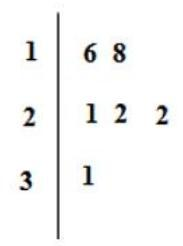
\includegraphics[max width=0.2\textwidth]{images/bo_d7fhnv491nqc73ercsbg_187_1280_560_183_246_0.jpg}
\end{center}
\hspace*{3em} 

\section*{四、统计}

1.(2025 高三二模青浦 4)如图是 6 株果树植株挂果个数(两位数)的茎叶图， 则 6 株果数植株挂果个数的中位数为\_\_\_\_\_.

【答案】 21.5

【解析】中位数为 \(\frac{{21} + {22}}{2} = {21.5}\) .

\begin{center}
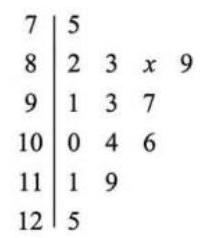
\includegraphics[max width=0.2\textwidth]{images/bo_d7fhnv491nqc73ercsbg_187_1270_849_203_238_0.jpg}
\end{center}
\hspace*{3em} 

2.(2025 高三二模崇明 7)某次数学考试后，随机选取 14 位学生的成绩，得到如下茎叶图, 其中个位数部分作为“叶”, 百位数和十位数作为“茎”, 若该组数据的第 25 百分位数是 87 , 则 \(x\) 的值为\_\_\_\_\_.

【答案】 7

【解析】由题意知 \({14} \times  {25}\%  = {3.5}\) ,则第四位数为 87,则 \(x = 7\)

3.(2025 高三二模闵行 7)已知数据 \({x}_{1}\text{ 、 }{x}_{2}\text{ 、 }\cdots \text{ 、 }{x}_{100}\) 的平均数为 2，方差为 5，则 \({x}_{1}^{2}\text{ 、 }{x}_{2}^{2}\) 、 \(\cdots \text{ 、 }{x}_{100}^{2}\) 的平均数为\_\_\_\_\_.

【答案】 9

【解析】由题意知 \(\frac{{x}_{1} + {x}_{2} + \cdots  + {x}_{100}}{100} = 2 \Rightarrow  {x}_{1} + {x}_{2} + \cdots  + {x}_{100} = {200}\) , \(\frac{{\left( {x}_{1} - 2\right) }^{2} + {\left( {x}_{2} - 2\right) }^{2} + \cdots  + {\left( {x}_{100} - 2\right) }^{2}}{100} = 5 \Rightarrow  {\left( {x}_{1} - 2\right) }^{2} + {\left( {x}_{2} - 2\right) }^{2} + \cdots  + {\left( {x}_{100} - 2\right) }^{2} = {500}\) , \(\therefore {x}_{1}^{2} + {x}_{2}^{2} + \cdots {x}_{100}{}^{2} - 4\left( {{x}_{1} + {x}_{2} + \cdots  + {x}_{100}}\right)  + 4 \times  {100} = {500}\) , \(\therefore {x}_{1}^{2} + {x}_{2}^{2} + \cdots {x}_{100}^{2} = {500} - {400} + 4\left( {{x}_{1} + {x}_{2} + \cdots  + {x}_{100}}\right)  = {100} + 4 \times  {200} = {900}\) , \(\therefore \frac{{x}_{1}^{2} + {x}_{2}^{2} + \cdots {x}_{100}^{2}}{100} = 9\) .

4.(2025 高三二模浦东 9)李老师在整理建模小组 10 名学生的成绩时不小心遗失了一位学生的成绩, 且剩余学生的成绩数据如下: 5 6 6 7 7 7 8 9 9 ，但李老师记得这名学生的成绩恰好是本组学生的第 25 百分位数，则这 10 名学生的成绩的方差为\_\_\_\_\_.

【答案】 \(\frac{8}{5}\)

【解析】 \(9 \times  {25}\%  = {2.25}\) ,即第三个学生的成绩 6 分位遗失分数学生的成绩,

此时 \(\bar{x} = \frac{5 + 6 + 6 + 6 + 7 + 7 + 7 + 8 + 9 + 9}{10} = 7\) ,

所以 \({s}^{2} = \frac{{5}^{2} + {6}^{2} + {6}^{2} + {6}^{2} + {7}^{2} + {7}^{2} + {7}^{2} + {8}^{2} + {9}^{2} + {9}^{2}}{10} - {7}^{2} = \frac{8}{5}\) .

5. (2025 高三二模普陀 13) 某市职业技能大赛的移动机器人比赛项目有 19 位同学参赛, 他们在预赛中所得的积分互不相同, 只有积分在前 10 位的同学才能进入决赛, 若该比赛项目中的某同学知道自己的积分后, 要判断自己能否进入决赛, 则他只需要知道这 19 位同学的预赛积分的( )

A. 平均数 B. 众数 C. 中位数 D. 方差

【答案】C

【解析】因为 19 为同学的积分各不相同, 则中位数即为排名第 10 的同学的积分, 则积分大于等于中位数可进入决赛, 积分小于中位数则无法进入决赛, 故选 C.

6.(2025 高三二模金山 14)某人统计了甲、乙两家零售商店在周一到周五的营业额(单位: 百元) 情况，得到了如下的茎叶图(其中茎表示十位数，叶表示个位数)，关于这 5 天的营业额情况，下列结论正确的是( )

\begin{center}
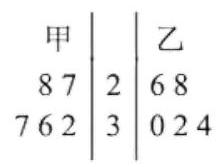
\includegraphics[max width=0.2\textwidth]{images/bo_d7fhnv491nqc73ercsbg_188_1096_860_216_167_0.jpg}
\end{center}
\hspace*{3em} 

第 14 题 图

A. 甲、乙两家商店营业额的极差相同

B. 甲、乙两家商店营业额的中位数相同

C. 从营业额超过 3000 元的天数所占比例来看，甲商店较高

D. 甲商店营业额的方差小于乙商店营业额的方差

【答案】C

【解析】由题意知甲组的数值依次为27,28,32,36,37,则极差为 \({37} - {27} = {10}\) ,中位数为

32,方差为 16.4,乙组的数值依次为26,28,30,32,34,则极差为 \({34} - {26} = 8\) ,中位数为

30，方差为 8 ，故选 C.

7. (2025 高三二模宝山 15)甲、乙两名篮球运动员在 8 场比赛中的单场得分用茎叶图表示如左下图, 茎叶图中甲的得分有部分数据丢失, 但甲得分的折线图完好 (右下图), 则下列结论正确的是 ( )

\begin{center}
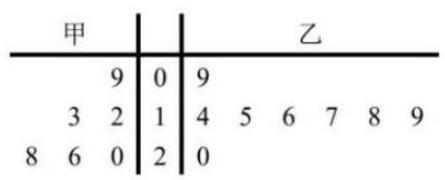
\includegraphics[max width=0.3\textwidth]{images/bo_d7fhnv491nqc73ercsbg_188_279_1568_445_180_0.jpg}
\end{center}
\hspace*{3em} 

\begin{center}
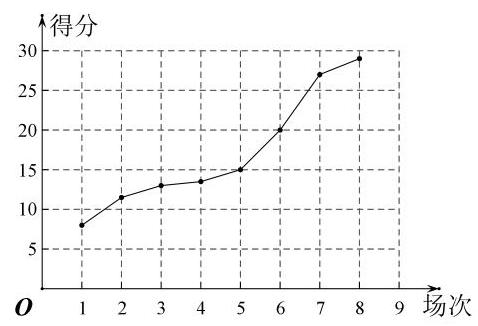
\includegraphics[max width=0.4\textwidth]{images/bo_d7fhnv491nqc73ercsbg_188_857_1492_478_326_0.jpg}
\end{center}
\hspace*{3em} 

A. 甲得分的极差小于乙得分的极差

B. 甲得分的第 25 百分位数大于乙得分的第 75 百分位数

C. 甲得分的平均数大于乙得分的平均数

D. 甲得分的方差小于乙得分的方差

【答案】C

【解析】A. 甲的极差为 \({28} - 9 = {19}\) ,乙的极差 \({20} - 9 = {11}\) ,所以 \(\mathrm{A}\) 错误;

B. \(8 \times  {25}\%  = 2\) ，所以第二个数字和第三个数字的平均数 \(\frac{{12} + {13}}{2} = {12.5}\) 为甲的第 25 百分位数, \(8 \times  {75}\%  = 6\) ,所以第六个数字和第七个数字的平均数 \(\frac{{18} + {19}}{2} = {18.5}\) 为乙的第 75 百分位数，所以 B 错误；

C. 由折线图可知甲的平均数为 \(\frac{9 + {12} + {13} + {14} + {15} + {20} + {26} + {28}}{8} = \frac{137}{8}\) ,

由茎叶图可知乙的平均数为 \(\frac{9 + {14} + {15} + {16} + {17} + {18} + {19} + {20}}{8} = {16}\) ,所以 \(\mathrm{C}\) 正确;

D. 甲的方差为 \(\frac{{9}^{2} + {12}^{2} + {13}^{2} + {14}^{2} + {15}^{2} + {20}^{2} + {26}^{2} + {28}^{2}}{8} - {\left( \frac{137}{8}\right) }^{2} = \frac{2631}{64}\) ,

乙的方差为 \(\frac{{9}^{2} + {14}^{2} + {15}^{2} + {16}^{2} + {17}^{2} + {18}^{2} + {19}^{2} + {20}^{2}}{8} - {16}^{2} = \frac{21}{2}\) ,

\begin{center}
\adjustbox{max width=\textwidth}{
\begin{tabular}{|c|c|c|c|}
\hline
\phantom{X} & \({y}_{1}\) & \({y}_{2}\) & 总计 \\
\cline{1-4}
\({x}_{1}\) & \(a\) & 35 & 45 \\
\cline{1-4}
\({x}_{2}\) & 7 & \(b\) & \(n\) \\
\cline{1-4}
总计 & m & 73 & \(S\) \\
\cline{1-4}
\hline
\end{tabular}
}
\end{center}

所以 D 错误;

故选 C.

\section*{五、成对数据的统计分析}

1.(2025 高三二模徐汇 5)右图是一个 \(2 \times  2\) 列联表，则 \(s =\) \_\_\_\_\_.

【答案】 90

【解析】由题意知

\(a = {45} - {35} = {10},m = {10} + 7 = {17},s = m + {73} = {17} + {73} = {90}.\)

2.(2025 高三二模长宁 5)为了研究吸烟习惯与慢性气管炎患病的关系，某疾病预防中心对相关调查数据进行了研究,假设 \({H}_{0}\) : 患慢性气管炎与吸烟没有关系,并通过计算得到统计量 \({\chi }^{2} \approx  {3.468}\) ，则可推断\_\_\_\_\_原假设 \({H}_{0}\) .(填“拒绝”或“接受”，规定显著水平 \(\alpha  = {0.1}\) ， \(P\left( {{\chi }^{2} \geq  {2.706}}\right)  \approx  {0.1}\) )

【答案】拒绝

【解析】显著水平 \(\alpha  = {0.1},{\chi }^{2} \approx  {3.468} > {2.706}\) ,所以拒绝原假设.

3.(2025 高三二模虹口 6)某公司为了解用电量 \(y\) (单位:千瓦时)与气温 \(x\) (单位:摄氏度) 之间的关系，随机统计了 4 天的用电量与当天气温，绘制了如右表格,由表中数据可得回归方程 \(y =  - {2x} + {59}\) ,则实数 \(m =\) \_\_\_\_\_.

\begin{center}
\adjustbox{max width=\textwidth}{
\begin{tabular}{|c|c|c|c|c|}
\hline
\(x\) & -1 & 10 & 13 & 18 \\
\cline{1-5}
\(y\) & 62 & 38 & 34 & m \\
\cline{1-5}
\hline
\end{tabular}
}
\end{center}

【答案】 24

【解析】由题意知样本点的中心为 \(\left( {\frac{-1 + {10} + {13} + {18}}{4},\frac{{62} + {38} + {34} + m}{4}}\right)\) ,即 \(\left( {{10},\frac{{134} + m}{4}}\right)\) 样本点的中心在回归方程上,即 \(- 2 \times  {10} + {59.5} = \frac{{134} + m}{4} \Rightarrow  m = {24}\) .

4.(2025 高三二模松江 6)根据右表所示的样本数据，用最小二乘法求得线性回归方程为 \(y = \widehat{a}x + {10.3}\) ，则回归系数 \(\widehat{a}\) 的值为\_\_\_\_\_.

\begin{center}
\adjustbox{max width=\textwidth}{
\begin{tabular}{|c|c|c|c|c|c|}
\hline
\(x\) & 6 & 8 & 9 & 10 & 12 \\
\cline{1-6}
\(y\) & 6 & 5 & 4 & 3 & 2 \\
\cline{1-6}
\hline
\end{tabular}
}
\end{center}

【答案】 -0.7

【解析】由题意 \(\bar{x} = \frac{6 + 8 + 9 + {10} + {12}}{5} = 9,\bar{y} = \frac{6 + 5 + 4 + 3 + 2}{5} = 4\) ,将样本中心点 \(\left( {\bar{x},\bar{y}}\right)\) 代入回归方程可得 \(\widehat{a} =  - {0.7}\) .

5.(2025 高三二模杨浦 9)植物社团的同学观察一株植物的生长情况，为了解植物高度 \(y\) (单位:厘米) 与生长期 \(x\) (单位:天)之间的关系，随机统计了某 4 天的植物高度，并制作了如下对照表:

\begin{center}
\adjustbox{max width=\textwidth}{
\begin{tabular}{|c|c|c|c|c|}
\hline
生长期 \(x\) & 3 & 9 & 11 & 17 \\
\cline{1-5}
植物高度 \(y\) & 2.4 & 3.4 & 3.8 & 5.2 \\
\cline{1-5}
\hline
\end{tabular}
}
\end{center}

由表中数据可得回归方程 \(y = \widehat{a}x + \widehat{b}\) 中 \(\widehat{a} = {0.2}\) ,试预测生长期是 30 天时,植物高度约为\_\_\_\_\_厘米. \(\left( {\widehat{a} = \frac{\mathop{\sum }\limits_{{i = 1}}^{n}{x}_{i}{y}_{i} - n\bar{x}\bar{y}}{\mathop{\sum }\limits_{{i = 1}}^{n}{x}_{i}^{2} - n{\bar{x}}^{2}},\widehat{b} = \bar{y} - \widehat{a}\bar{x}}\right)\)

【答案】 7.7

【解析】 \(\bar{x} = \frac{3 + 9 + {11} + {17}}{4} = {10},\bar{y} = \frac{{2.4} + {3.4} + {3.8} + {5.2}}{4} = {3.7}\) ,代入回归方程解得 \(\widehat{b} = {1.7}\) ,当 \(x = {30}\) 时, \(y = {0.2} \times  {30} + {1.7} = 6 + {1.7} = {7.7}\) 厘米.

6. (2025 高三二模奉贤 9) 通过随机抽样, 获得某种商品消费者年需求量与该商品每千克价格之间的一组数据调查，如下表所示:

\begin{center}
\adjustbox{max width=\textwidth}{
\begin{tabular}{|c|c|c|c|c|c|c|c|c|c|c|}
\hline
价格 (百元) & \({x}_{1}\) & \({x}_{2}\) & \({x}_{3}\) & \({x}_{4}\) & \({x}_{5}\) & \({x}_{6}\) & \({x}_{7}\) & \({x}_{8}\) & \({x}_{9}\) & \({x}_{10}\) \\
\cline{1-11}
\phantom{X} & 4 & 4 & 4.6 & 5 & 5.2 & 5.6 & 6 & 6.6 & 7 & 10 \\
\cline{1-11}
需求量(千克) & \({y}_{1}\) & \({y}_{2}\) & \({y}_{3}\) & \({y}_{4}\) & \({y}_{5}\) & \({y}_{6}\) & \({y}_{7}\) & \({y}_{8}\) & \({y}_{9}\) & \({y}_{10}\) \\
\cline{1-11}
\phantom{X} & 3.5 & 3 & 2.7 & 2.4 & 2.5 & 2 & 1.5 & 1.2 & 1.2 & 1 \\
\cline{1-11}
\hline
\end{tabular}
}
\end{center}

那么线性相关系数 \(r =\) \_\_\_\_\_. (精确到 0.001 )

线性相关系数公式 \(r = \frac{\mathop{\sum }\limits_{{i = 1}}^{n}\left( {{x}_{i} - \bar{x}}\right) \left( {{y}_{i} - \bar{y}}\right) }{\sqrt{\mathop{\sum }\limits_{{i = 1}}^{n}{\left( {x}_{i} - \bar{x}\right) }^{2} \cdot  \mathop{\sum }\limits_{{i = 1}}^{n}{\left( {y}_{i} - \bar{y}\right) }^{2}}}\)

【答案】 -0.863

【解析】通过计算器的统计功能即可得.

7.(2025 高三二模闵行 13)两个变量 \(x\) 与 \(y\) 之间的回归方程( ).

A.表示 \(x\) 与 \(y\) 之间的函数关系 B.表示 \(x\) 与 \(y\) 之间的不确定关系

C. 反映 \(x\) 与 \(y\) 之间的真实关系 D. 是反映 \(x\) 与 \(y\) 之间的真实关系的一种最佳拟合

【答案】D

【解析】由回归方程的定义可知选 D.

8.(2025 高三二模黄浦 13)如果两种证券在一段时间内收益数据的相关系数为 0.8 ，那么表明 ( )

A. 两种证券的收益有反向变动的倾向

B. 两种证券的收益有同向变动的倾向

C. 两种证券的收益之间存在完全反向的联动关系, 即涨或跌是相反的

D. 两种证券的收益之间存在完全同向的联动关系, 即同时涨或同时跌

【答案】B

【解析】因为相关系数 \({0.8} > 0\) ,所以两种收益为正相关,故 AC 错误,当相关系数为 1 时, 两种收益为完全相同的联动关系, \({0.8} < 1\) ，所以 D 错误，故选 B.

9.(2025 高三二模长宁 14)某书店为了分析书籍销量与宣传投入之间的关系，对宣传投入 \(x\) (千元)和书籍销量 \(y\) (百本)的情况进行了调研，并统计得到右表中几组对应数据，同时用最小二乘法得到 \(y\) 关于 \(x\) 的线性回归方程为 \(y = {1.2x} + {1.6}\) ,则下列说法不正确的是 ( )

\begin{center}
\adjustbox{max width=\textwidth}{
\begin{tabular}{|c|c|c|c|c|}
\hline
\(x\) & 3 & 4 & 5 & 6 \\
\cline{1-5}
\(y\) & 5 & 6.2 & 7.4 & \(m\) \\
\cline{1-5}
\hline
\end{tabular}
}
\end{center}

A. 变量 \(x\) 、 \(y\) 之间呈正相关

B. 预测当宣传投入 2 千元时, 书籍销量约为 400 本

C. \(m = {8.8}\)

D. 拟合误差 \(Q = {0.48}\)

【答案】C

【解析】A.线性回归方程 \(x\) 的系数 \({1.2} > 0\) ,所以 \(x\text{ 、 }y\) 之间呈正相关,正确;

B. 将 \(x = 2\) 代入线性回归方程，解得 \(y = 4\) ，可知销量约为 400 本，正确；

C. 样本中心点在回归方程上， \(\overset{ - }{x} = \frac{3 + 4 + 5 + 6}{4} = {4.5},\overset{ - }{y} = \frac{5 + {6.2} + {7.4} + m}{4} = \frac{{18.6} + m}{4}\) 则 \(\frac{{18.6} + m}{4} = {1.2} \times  {4.5} + {1.6} \Rightarrow  m = {9.4}\) ,所以 \(\mathrm{C}\) 错误;

D. 拟合误差 \(Q = \mathop{\sum }\limits_{{i = 1}}^{n}{\left( {y}_{i} - {\widehat{y}}_{i}\right) }^{2},{\widehat{y}}_{1} = {1.2} \times  3 + {1.6} = {5.2},{\widehat{y}}_{2} = {1.2} \times  4 + {1.6} = {6.4}\) ,

\({\widehat{y}}_{3} = {1.2} \times  5 + {1.6} = {7.6},\;{\widehat{y}}_{4} = {1.2} \times  6 + {1.6} = {8.8},\)

所以 \(Q = {\left( 5 - {5.2}\right) }^{2} + {\left( {6.2} - {6.4}\right) }^{2} + {\left( {7.4} - {7.6}\right) }^{2} + {\left( {9.4} - {8.8}\right) }^{2} = {0.48}\) ,正确; 故选 C.

10.(2025 高三二模徐汇 14)在研究线性回归模型时，若样本数据 \(\left( {{x}_{i},{y}_{i}}\right) \left( {i = 1,2,3,\cdots ,n}\right)\) 所对应的点都在直线 \(y =  - \frac{1}{3}x + 2\) 上,则两组数据 \({x}_{i}\) 和 \({y}_{i}\left( {i = 1,2,3,\cdots ,n}\right)\) 的线性相关系数为 ( )

A. -1 B. 1

C. \(- \frac{1}{3}\) D. 2

【答案】A

【解析】若样本数据所对应的点都在直线上,则相关性最强,且 \(\left| r\right|  = 1\) ,

又因为是负相关,则 \(r =  - 1\) ,故选 A.

11.(2025 高三二模浦东 15)研究变量 \(x,y\) 得到一组成对数据 \(\left( {{x}_{i},{y}_{i}}\right) ,i = 1,2,\cdots ,n\) ，先进行一次线性回归分析,接着增加一个数据 \(\left( {{x}_{n + 1},{y}_{n + 1}}\right)\) ,其中 \({x}_{n + 1} = \frac{1}{n}\mathop{\sum }\limits_{{i = 1}}^{n}{x}_{i},{y}_{n + 1} = \frac{1}{n}\mathop{\sum }\limits_{{i = 1}}^{n}{y}_{i}\) , 再重新进行一次线性回归分析, 则下列说法正确的是 ( )

A. 变量 \(x\) 与变量 \(y\) 的相关性变强 B. 相关系数 \(r\) 的绝对值变小

C. 线性回归方程 \(y = \widehat{a}x + \widehat{b}\) 不变 D. 拟合误差 \(Q\) 变大

【答案】C

【解析】因为 \({x}_{n + 1} = \frac{1}{n}\mathop{\sum }\limits_{{i = 1}}^{n}{x}_{i},{y}_{n + 1} = \frac{1}{n}\mathop{\sum }\limits_{{i = 1}}^{n}{y}_{i}\) ,所以增加的数据 \(\left( {{x}_{n + 1},{y}_{n + 1}}\right)\) 为原数据的样本中心点, 在线性回归方程上, 故加入这个数据, 线性回归方程不变, 故选 C.

12.(2025 高三二模奉贤 17)某疾病预防中心随机调查了 339 名 50 岁以上的公民，研究吸烟习惯与慢性气管炎患病的关系，测得数据如表所示:

\begin{center}
\adjustbox{max width=\textwidth}{
\begin{tabular}{|c|c|c|c|}
\hline
\phantom{X} & 不吸烟者 & 吸烟者 & 总计 \\
\cline{1-4}
不患慢性气管炎者 & 121 & \(b\) & 283 \\
\cline{1-4}
患慢性气管炎者 & \(C\) & \(d\) & \phantom{X} \\
\cline{1-4}
总计 & 134 & \phantom{X} & 339 \\
\cline{1-4}
\hline
\end{tabular}
}
\end{center}

(1)估算样本中吸烟者中患慢性支气管炎的百分比；

(2)有多少把握认为患慢性支气管炎与吸烟有关？

附: \({\chi }^{2} = \frac{n{\left( ad - bc\right) }^{2}}{\left( {a + b}\right) \left( {c + d}\right) \left( {a + c}\right) \left( {b + d}\right) }\) ，其中 \(n = a + b + c + d\)

\[
P\left( {{\chi }^{2} \geq  {6.635}}\right)  \approx  {0.01},P\left( {{\chi }^{2} \geq  {5.024}}\right)  \approx  {0.025},
\]

\[
P\left( {{\chi }^{2} \geq  {3.841}}\right)  \approx  {0.05},\;P\left( {{\chi }^{2} \geq  {2.706}}\right)  \approx  {0.1}.
\]

【答案】(1)26.54\%；(2)有99\%把握

【解析】(1) 由已知, \(t = {205},m = {43}\)

所以，估算样本中吸烟者约有 26.54\%患有慢性支气管炎。 6 分

(2)假设患慢性支气管炎与吸烟无关，计算 \({\chi }^{2}\)

\[
{\chi }^{2} = \frac{n{\left( ad - bc\right) }^{2}}{\left( {a + b}\right) \left( {c + d}\right) \left( {a + c}\right) \left( {b + d}\right) } = \frac{{339}{\left( {121} \times  {43} - {162} \times  {13}\right) }^{2}}{{283} \times  {56} \times  {134} \times  {205}} \approx  {7.468}
\]

\[
{\chi }^{2} \approx  {7.468} > {6.635}
\]

所以我们有 99\% 把握认为患慢性支气管炎与吸烟有关. 4 分

\section*{六、概率统计综合}

1.(2025高三二模静安18)某校高三共有300名学生，分六个班，每班50人.为了解该校高三学生的视力情况，体检后每班按随机抽样的方法抽取了8名学生的视力数据. 其中高三(1) 班抽取的 8 名学生的视力数据与人数见下表:

(1)用上述样本数据估计高三(1)班学生视力的平均值；

(2)已知其余五个班学生视力的平均值分别为 \({4.3}\text{ 、 }{4.4}\text{ 、 }{4.5}\text{ 、 }{4.6}\text{ 、 }{4.8}\) . 若从这六个班中任意抽取两个班学生视力的平均值作比较, 求抽取的两个班学生视力的平均值之差的绝对值不小于 0.2 的概率.

【答案】(1) 4.7; (2) \(\frac{2}{3}\)

【解析】(1) 高三(1)班抽取的 8 名学生视力的平均值为

\(\frac{{4.4} \times  2 + {4.6} \times  2 + {4.8} \times  2 + {4.9} + {5.1}}{8} = {4.7}.\)

据此估计高三(1)班学生视力的平均值约为 4.7. (6 分)

(2)因为高三六个班学生视力的平均值分别为 \({4.3}\text{ 、 }{4.4}\text{ 、 }{4.5}\text{ 、 }{4.6}\text{ 、 }{4.7}\text{ 、 }{4.8}\) ，

所以任意抽取两个班学生视力的平均值数对有:

\(\left( {{4.3},{4.4}}\right) ,\left( {{4.3},{4.5}}\right) ,\left( {{4.3},{4.6}}\right) ,\left( {{4.3},{4.7}}\right) ,\left( {{4.3},{4.8}}\right) ,\left( {{4.4},{4.5}}\right) ,\left( {{4.4},{4.6}}\right)\) ,

\(\left( {{4.4},{4.7}}\right) ,\left( {{4.4},{4.8}}\right) ,\left( {{4.5},{4.6}}\right) ,\left( {{4.5},{4.7}}\right) ,\left( {{4.5},{4.8}}\right) ,\left( {{4.6},{4.7}}\right) ,\left( {{4.6},{4.8}}\right)\) ,

(4.7, 4.8) 共 15 种情形; (3 分)

其中抽取的两个班学生视力的平均值之差的绝对值不小于 0.2 的有

\(\left( {{4.3},{4.5}}\right) ,\left( {{4.3},{4.6}}\right) ,\left( {{4.3},{4.7}}\right) ,\left( {{4.3},{4.8}}\right) ,\left( {{4.4},{4.6}}\right) ,\left( {{4.4},{4.7}}\right) ,\left( {{4.4},{4.8}}\right)\) , \(\left( {{4.5},{4.7}}\right) ,\left( {{4.5},{4.8}}\right) ,\left( {{4.6},{4.8}}\right)\) ,共 10 种. (3 分)

所以抽取的两个班学生视力的平均值之差的绝对值不小于 0.2 的概率为 \(\frac{10}{15} = \frac{2}{3}\) . (2 分)

2.(2025 高三二模虹口 19)已知某区组建了一支 120 人的志愿者队伍，并由其中 72 人组成 “志愿模范队”. 经过一年的实践，全队共有 72 人的周平均服务时长超过 2 小时，其中有 54 人来自“志愿模范队”，如下表所示.

\begin{center}
\adjustbox{max width=\textwidth}{
\begin{tabular}{|c|c|c|c|}
\hline
\phantom{X} & 是“志愿模范队”成员 & 不是“志愿模范队”成员 & 总计 \\
\cline{1-4}
周平均服务时长超过 2 小时 & 54 & \phantom{X} & 72 \\
\cline{1-4}
周平均服务时长不超过 2 小时 & \phantom{X} & \phantom{X} & \phantom{X} \\
\cline{1-4}
总计 & 72 & \phantom{X} & 120 \\
\cline{1-4}
\hline
\end{tabular}
}
\end{center}

(1)已知一名志愿者是“志愿模范队”成员，求其周平均服务时长超过 2 小时的概率.

(2)请完成 \(2 \times  2\) 列联表，并根据表中数据回答:是否有 99.9\%的把握认为“是‘志愿模范队’ 成员”与“周平均服务时长超过 2 小时”有关系?

(3)现从周平均服务时长超过 2 小时的人员中按照是否为“志愿模范队”进行分层抽样选取 8 人组建“志愿突击队”，并从这 8 人中随机选取 2 人做深度访谈，记随机变量 \(X\) 为这 2 人中来自于“志愿模范队”的人数，求 \(X\) 的分布与方差.

\begin{center}
\adjustbox{max width=\textwidth}{
\begin{tabular}{|c|c|c|c|c|}
\hline
\(P\left( {{\chi }^{2} \geq  k}\right)\) & 0.100 & 0.050 & 0.010 & 0.001 \\
\cline{1-5}
\(k\) & 2.706 & 3.841 & 6.635 & 10.828 \\
\cline{1-5}
\hline
\end{tabular}
}
\end{center}

附录: \({\chi }^{2} = \frac{n{\left( ad - bc\right) }^{2}}{\left( {a + b}\right) \left( {c + d}\right) \left( {a + c}\right) \left( {b + d}\right) }\) ,

其中 \(n = a + b + c + d\) .

【答案】(1) \(\frac{3}{4}\) ; (2) 有99.9\%的把握; (3) \(X\) 的分布为 \(\left( \begin{matrix} 0 & 1 & 2 \\  \frac{1}{28} & \frac{3}{7} & \frac{15}{28} \end{matrix}\right)\) , \(D\left\lbrack  X\right\rbrack   = \frac{9}{28}.\)

【解析】(1)事件 \(A\) 表示志愿者是“志愿模范队”成员,事件 \(B\) 表示其周平均服务时长超过 2 小时. 则 \(P\left( {B \mid  A}\right)  = \frac{P\left( {A \cap  B}\right) }{P\left( A\right) } = \frac{\frac{54}{120}}{\frac{72}{120}} = \frac{3}{4}\) . .2 分

(2)可得如下 \(2 \times  2\) 列联表:

\begin{center}
\adjustbox{max width=\textwidth}{
\begin{tabular}{|c|c|c|c|}
\hline
\phantom{X} & 是“志愿模范队”成员 & 不是“志愿模范队”成员 & 总计 \\
\cline{1-4}
周平均服务时长超过 2 小时 & 54 & 18 & 72 \\
\cline{1-4}
周平均服务时长不超过 2 小时 & 18 & 30 & 48 \\
\cline{1-4}
总计 & 72 & 48 & 120 \\
\cline{1-4}
\hline
\end{tabular}
}
\end{center}

提出原假设 \({H}_{0}\) : 是否“是‘志愿模范队’成员”与“周平均服务时长超过 2 小时”无关，确定显著性水平 \(\alpha  = {0.001}\) . .4 分

可得 \({\chi }^{2} = \frac{{120}{\left( {54} \times  {30} - {18} \times  {18}\right) }^{2}}{{72}\;{48}\;{72}\;{48}} = \frac{135}{8} = {16.875}\) . .6 分

由于 \({\chi }^{2} > {10.828}\) ,拒绝原假设,即有 99.9\% 的把握认为 “是‘志愿模范队’成员”与“周平均服务时长超过 2 小时”有关. .8 分

(3)根据 \(2 \times  2\) 列联表可得“志愿模范队”成员中“周平均服务时长超过 2 小时”占全部的 \(\frac{54}{72} = \frac{3}{4}\) . 选取的 8 人中“周平均服务时长超过 2 小时”为 6 人，“周平均服务时长不超过 2 小时”为 2 人， \(X = 0,1,2\) .

\(P\left( {X = 0}\right)  = \frac{{C}_{6}^{0}{C}_{2}^{2}}{{C}_{8}^{2}} = \frac{1}{28},P\left( {X = 1}\right)  = \frac{{C}_{6}^{1}{C}_{2}^{1}}{{C}_{8}^{2}} = \frac{3}{7},P\left( {X = 2}\right)  = \frac{{C}_{6}^{2}{C}_{2}^{0}}{{C}_{8}^{2}} = \frac{15}{28}.\)

\(X\) 的分布为 \(\left( \begin{matrix} 0 & 1 & 2 \\  \frac{1}{28} & \frac{3}{7} & \frac{15}{28} \end{matrix}\right)\) . .10 分

\(E\left\lbrack  X\right\rbrack   = 0 \times  \frac{1}{28} + 1 \times  \frac{3}{7} + 2 \times  \frac{15}{28} = \frac{3}{2}.\) .12 分

又由于 \(E\left\lbrack  {X}^{2}\right\rbrack   = \frac{18}{7}\) . 所以 \(D\left\lbrack  X\right\rbrack   = E\left\lbrack  {X}^{2}\right\rbrack   - {\left( E\left\lbrack  X\right\rbrack  \right) }^{2} = \frac{9}{28}\) . .14 分

3. (2025 高三二模宝山 19)某游乐园的活动项目共有三类，分别是“过山车”等 10 个体验类项目、“海豚之舞”等 4 个表演类项目、“智力闯关”等 3 个互动类项目. 因设备维护需要，项目并非每日都全部开放. 以下数据是项目开放的数量 \(x\) (个) 和游客平均等待时间 \(t\) (分钟/个) 的关系:

\begin{center}
\adjustbox{max width=\textwidth}{
\begin{tabular}{|c|c|c|c|c|c|c|c|c|c|}
\hline
项目类别 & \multicolumn{5}{|c|}{体验类} & \multicolumn{2}{|c|}{演出类} & \multicolumn{2}{|c|}{互动类} \\
\cline{1-10}
开放数量 \(x\) (个) & 4 & 5 & 6 & 7 & 8 & 2 & 4 & 2 & 3 \\
\cline{1-10}
平均等待时间 \(y\) (分钟/个) & 76 & 73 & 67 & \(m\) & 60 & 53 & 30 & 46 & 30 \\
\cline{1-10}
\hline
\end{tabular}
}
\end{center}

(1)体验类项目中,若 \(y\) 关于 \(x\) 波动的回归方程为 \(y =  - {4.3x} + {93.8}\) ,请计算 \(m\) 的值,并依据该模型预测所有体验类项目均开放时的平均等待时间 (精确到整数);

(2)小王游玩当日，体验类、演出类、互动类项目分别开放了 8 个、 4 个、3 个，他计划随机游玩其中的 3 个项目, 已知他选择的项目中至少包含 1 个互动类项目, 求他的等待总时间恰为 120 分钟的概率;

(3)为提高游客的参与度，园方在互动类项目“智力闯关”中设计了两关.通过第一关的游客奖励 20 个游园币，游客可以选择结束或继续闯关. 若继续闯关，则必须完成第二关的所有题目.第二关包含 2 道相互独立的选择题, 每答对 1 题可再奖励 20 个游园币, 每答错 1 题则要扣除 10 个游园币.每个游园币可兑换园区内任意一个项目的 1 分钟等待时间.

小王已通过第一关，假设他在第二关中每道题答对的概率均为 \(p\) ，为了获得更多项目等待时间的兑换奖励，小王是否应该继续闯关？请你帮他做出决策.

【答案】(1) \(m = {64}\) ，开放所有体验类项目时的平均等待时间约为 51 分钟；(2) \(\frac{24}{47}\) ；(3) 当 \(0 \leq  p < \frac{1}{3}\) 时, \(E\left( X\right)  < 0\) ,不建议小王继续闯关; 当 \(p = \frac{1}{3}\) 时, \(E\left( X\right)  = 0\) ,小王可根据自己的情况随机选择; 当 \(\frac{1}{3} < p \leq  1\) 时, \(E\left( X\right)  > 0\) ,建议小王继续闯关.

【解析】(1) \(\bar{x} = \frac{4 + 5 + 6 + 7 + 8}{5} = 6,\bar{y} = \frac{{76} + {73} + {67} + m + {60}}{5} = \frac{m + {276}}{5}\) , .2 分代入回归方程 \(y =  - {4.3x} + {93.8}\) ，得: \(\frac{m + {276}}{5} =  - {4.3} \times  6 + {93.8}\) 解得 \(m = {64}\) ， .3 分 \(x = {10}\) 时 \(y =  - {4.3} \times  {10} + {93.8} = {50.8}\) ,

即开放所有体验类项目时的平均等待时间约为 51 分钟. .4 分

(2)事件 \(A\) : 等待总时间恰为 120 分钟;

事件 \(B\) : 选择的 3 个项目中至少包含 1 个互动类项目

全部的项目数为 15 个,其中互动类项目有 3 个,则事件 \(B\) 共包含了 \({C}_{15}^{3} - {C}_{12}^{3}\) 种;

.6 分

在事件 \(B\) 的条件下,等待总时间恰为 120 分钟,此时的可能情况是:

 \circled{1} 一个互动类项目，一个体验类项目，一个演出类项目，此时共有 \({C}_{3}^{1}{C}_{8}^{1}{C}_{4}^{1}\) 种情况；

 \circled{2} 两个互动类项目，一个体验类项目，此时共有 \({C}_{3}^{2}{C}_{8}^{1}\) 种情况. .8 分

由条件概率公式得

\[
P\left( {A \mid  B}\right)  = \frac{P\left( {A \cap  B}\right) }{P\left( B\right) } = \frac{\left| A \cap  B\right| }{\left| B\right| } = \frac{{C}_{3}^{2}{C}_{8}^{1} + {C}_{3}^{1}{C}_{4}^{1}{C}_{8}^{1}}{{C}_{15}^{3} - {C}_{12}^{3}} = \frac{24}{47}
\]

10 分

(3)事件 \(X = k\) 表示“小王参加决赛获得的游园币”，则

\(P\left( {X = {40}}\right)  = {p}^{2},P\left( {X = {10}}\right)  = {C}_{2}^{1}p\left( {1 - p}\right) ,P\left( {X =  - {20}}\right)  = {\left( 1 - p\right) }^{2}\) .13 分

所以 \(E\left( X\right)  = {40} \cdot  {P}^{2} + {10} \cdot  {C}_{2}^{1}p\left( {1 - p}\right)  + \left( {-{20}}\right)  \cdot  {\left( 1 - p\right) }^{2} = {60p} - {20}\) .14 分

所以,当 \(0 \leq  p < \frac{1}{3}\) 时, \(E\left( X\right)  < 0\) ,不建议小王继续闯关;

当 \(p = \frac{1}{3}\) 时, \(E\left( X\right)  = 0\) ,小王可根据自己的情况随机选择;

当 \(\frac{1}{3} < p \leq  1\) 时, \(E\left( X\right)  > 0\) ,建议小王继续闯关. 16 分

4. (2025 高三二模杨浦 19) 为弘扬中华民族传统文化、增强民族自豪感, 某学校开展中华古诗词背诵比赛，分为初赛和复赛. 全校同学都参加了初赛，并随机抽取一个班级进行初赛成绩统计, 已知该班级共有 40 位学生, 他们的比赛分数的频率分布直方图如图所示:

\begin{center}
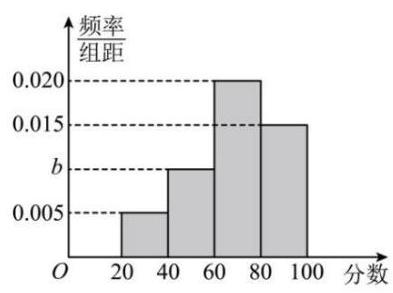
\includegraphics[max width=0.3\textwidth]{images/bo_d7fhnv491nqc73ercsbg_196_1009_1364_393_293_0.jpg}
\end{center}
\hspace*{3em} 

第 19 题图

(1)计算 \(b\) 的值，并估计该校这次比赛的平均分数.

(2)分数达到 80 及以上的同学，称为优秀参赛选手，现从班级中随机选出 2 位同学，用 \(X\) 代表其中的优秀参赛选手人数，求 \(X\) 的分布；

(3)为增加比赛的趣味性，复赛规则如下:比赛试题将从题库中随机抽取，每位参赛选手将有机会回答填空、选择和简答各 1 题; 每答对 1 题得 1 分, 答错或不答得 0 分, 每位选手可以自行选择回答问题的顺序, 若答对一题可继续答下一题, 直到 3 题全部答完; 若答错或不答则比赛结束. 例如: 选手甲可自行按“简答——填空——选择”顺序答题，甲答对第一题得 1 分, 并继续回答第二题且答错得 0 分, 结束比赛, 总分为 1 分.

小杨作为优秀参赛选手，代表班级参加复赛. 根据他初赛的答题正确频率，可估计他填空、 选择和简答的答题正确概率分别为:

\begin{center}
\adjustbox{max width=\textwidth}{
\begin{tabular}{|c|c|c|c|}
\hline
题型 & 填空 & 选择 & 简答 \\
\cline{1-4}
答题正确概率 & 80\% & 90\% & 80\% \\
\cline{1-4}
\hline
\end{tabular}
}
\end{center}

若小杨每次答题的结果都相互独立，那么为尽量在比赛中获得较高分数，小杨应该采用怎样的答题顺序? 请说明理由.

【答案】(1) \(b = {0.010}\) ,平均数为 68 分; (2) \(X\) 的分布为 \(\left( \begin{matrix} 0 & 1 & 2 \\  \frac{63}{130} & \frac{28}{65} & \frac{11}{130} \end{matrix}\right)\) ; (3) 选取方案二:“选择——填空——简答”或“选择——简答——填空”

【解析】(1) \(\left( {{0.005} + b + {0.015} + {0.02}}\right)  \times  {20} = 1\) ,计算得 \(b = {0.010}\) .2

\begin{center}
\adjustbox{max width=\textwidth}{
\begin{tabular}{|c|c|c|c|c|}
\hline
分数分组区间 & \(\lbrack {20},{40})\) & \(\lbrack {40},{60})\) & \(\lbrack {60},{80})\) & [80,100] \\
\cline{1-5}
频数 & 4 & 8 & 16 & 12 \\
\cline{1-5}
\hline
\end{tabular}
}
\end{center}

各区间的中点值: \({30}\text{ 、 }{50}\text{ 、 }{70}\text{ 、 }{90}\) ,

比赛分数的平均数为 \(\frac{{30} \times  4 + {50} \times  8 + {70} \times  {16} + {90} \times  {12}}{40} = {68}\) (分) .4

(2) \({0.0015} \times  {20} \times  {40} = {12}\) ，班级中优秀参赛选手的人数为 12 人 .5 \(X\) 的可能取值为 0、1、2,依题意,

\(P\left( {X = 0}\right)  = \frac{{\mathrm{C}}_{12}^{0}{\mathrm{C}}_{28}^{2}}{{\mathrm{C}}_{40}^{2}} = \frac{63}{130},\;P\left( {X = 1}\right)  = \frac{{\mathrm{C}}_{12}^{1}{\mathrm{C}}_{28}^{1}}{{\mathrm{C}}_{40}^{2}} = \frac{28}{65},\;P\left( {X = 2}\right)  = \frac{{\mathrm{C}}_{12}^{2}{\mathrm{C}}_{28}^{0}}{{\mathrm{C}}_{40}^{2}} = \frac{11}{130},\)

所以 \(X\) 的分布为 \(\left( \begin{matrix} 0 & 1 & 2 \\  \frac{63}{130} & \frac{28}{65} & \frac{11}{130} \end{matrix}\right)\) , .8

(3)答题顺序为:“选择一填空一简答”或“选择一简答——填空”，理由如下:

由于小杨“填空”和“简答”的答题正确率都为 80\%，考查“选择”的位置顺序.

得分 \(Y\) 的可能取值为: \(0\text{ 、 }1\text{ 、 }2\text{ 、 }3\) ,

方案一:“填空——选择——简答”或“简答——选择——填空”，

\(E\left\lbrack  Y\right\rbrack   = 0 \times  \left( {1 - {0.8}}\right)  + 1 \times  {0.8} \times  \left( {1 - {0.9}}\right)  + 2 \times  {0.8} \times  {0.9} \times  \left( {1 - {0.8}}\right)  + 3 \times  {0.8} \times  {0.9} \times  {0.8} = {2.096}\) .10

方案二:“选择——填空——简答”或“选择——简答——填空”，

\[
E\left\lbrack  Y\right\rbrack   = 0 \times  \left( {1 - {0.9}}\right)  + 1 \times  {0.9} \times  \left( {1 - {0.8}}\right)  + 2 \times  {0.9} \times  {0.8} \times  \left( {1 - {0.8}}\right)  + 3 \times  {0.9} \times  {0.8} \times  {0.8} = {2.196}
\]

.12

方案三:“填空——简答——选择”或“简答——填空——选择”，

\[
E\left\lbrack  Y\right\rbrack   = 0 \times  \left( {1 - {0.8}}\right)  + 1 \times  {0.8} \times  \left( {1 - {0.8}}\right)  + 2 \times  {0.8} \times  {0.8} \times  \left( {1 - {0.9}}\right)  + 3 \times  {0.8} \times  {0.8} \times  {0.9} = {2.016}.
\]

选取 \(E\left\lbrack  Y\right\rbrack\) 最大的方案,即方案二: “选择一填空一简答”或“选择一简答一填空”....14

5. (2025 高三二模青浦 19)某工厂生产某款电池，在满电状态下能够持续放电时间不低于 10 小时的为合格品, 工程师选择某台生产电池的机器进行参数调试, 在调试前后, 分别在其产品中随机抽取样本数据进行统计,制作了如下的 \(2 \times  2\) 列联表:

\begin{center}
\adjustbox{max width=\textwidth}{
\begin{tabular}{|c|c|c|c|}
\hline
产品 & 合格 & 不合格 & 合计 \\
\cline{1-4}
调试前 & 45 & 15 & 60 \\
\cline{1-4}
调试后 & 35 & 5 & 40 \\
\cline{1-4}
合计 & 80 & 20 & 100 \\
\cline{1-4}
\hline
\end{tabular}
}
\end{center}

(1)根据表中数据，依据显著性水平 \(\alpha  = {0.01}\) 的独立性检验，能否认为参数调试与产品质量有关联;

(2)现从调试前的样本中按合格和不合格，用分层随机抽样法抽取 8 件产品重新做参数调试,再从这 8 件产品中随机抽取 3 件做对比分析,记抽取的 3 件中合格的件数为 \(X\) ,求 \(X\) 的分布和期望;

(3)用样本分布的频率估计总体分布的概率，若现在随机抽取调试后的产品 1000 件，记其中合格的件数为 \(Y\) ,求使事件“ \(Y = k\) ”的概率最大时 \(k\) 的取值.

参考公式及数据: \({\chi }^{2} = \frac{n{\left( ad - bc\right) }^{2}}{\left( {a + b}\right) \left( {c + d}\right) \left( {a + c}\right) \left( {b + d}\right) }\) ,其中 \(n = a + b + c + d\) .

\begin{center}
\adjustbox{max width=\textwidth}{
\begin{tabular}{|c|c|c|c|c|c|}
\hline
\(P\left( {{\chi }^{2} \geq  {\chi }_{0}}\right)\) & 0.05 & 0.025 & 0.01 & 0.005 & 0.001 \\
\cline{1-6}
\({\chi }_{0}\) & 3.841 & 5.024 & 6.635 & 7.879 & 10.828 \\
\cline{1-6}
\hline
\end{tabular}
}
\end{center}

【答案】(1)参数调试与产品质量无关联；(2) \(X\) 的分布为: \(\left( \begin{matrix} 1 & 2 & 3 \\  \frac{3}{28} & \frac{15}{28} & \frac{10}{28} \end{matrix}\right)\)

\(E\left( X\right)  = \frac{9}{4};\left( 3\right) k = {875}\)

【解析】(1) 零假设为 \({H}_{0}\) : 假设依据 \(\alpha  = {0.01}\) 的独立性检验,认为参数调试与产品质量无关联; 则 \({\chi }^{2} = \frac{{100}{\left( {45} \times  5 - {35} \times  {15}\right) }^{2}}{{80} \times  {20} \times  {40} \times  {60}} \approx  {2.344} < {x}_{0.01} = {6.635}\) ,

故依据 \(\alpha  = {0.01}\) 的独立性检验,没有充分证据说明零假设 \({H}_{0}\) 不成立,

因此可认为 \({H}_{0}\) 成立,即认为参数调试与产品质量无关联;

(2)依题意，用分层随机抽样法抽取的 8 件产品中，

合格产品有 \(8 \times  \frac{45}{60} = 6\) 件，不合格产品有 2 件，

而从这 8 件产品中随机抽取 3 件,其中的合格品件数 \(X\) 的可能值有1,2,3.

则 \(P\left( {X = 1}\right)  = \frac{{\mathrm{C}}_{6}^{1}{\mathrm{C}}_{2}^{2}}{{\mathrm{C}}_{8}^{3}} = \frac{3}{28},P\left( {X = 2}\right)  = \frac{{\mathrm{C}}_{6}^{2}{\mathrm{C}}_{2}^{1}}{{\mathrm{C}}_{8}^{3}} = \frac{15}{28},P\left( {X = 3}\right)  = \frac{{\mathrm{C}}_{6}^{3}{\mathrm{C}}_{2}^{0}}{{\mathrm{C}}_{8}^{3}} = \frac{10}{28}\) .

故 \(X\) 的分布为: \(\left( \begin{matrix} 1 & 2 & 3 \\  \frac{3}{28} & \frac{15}{28} & \frac{10}{28} \end{matrix}\right)\)

则 \(E\left( X\right)  = 1 \times  \frac{3}{28} + 2 \times  \frac{15}{28} + 3 \times  \frac{10}{28} = \frac{9}{4}\) ;

(3)依题意，因随机抽取调试后的产品的合格率为 \(\frac{35}{40} = \frac{7}{8}\) ，故 \(Y \sim  B\left( {{1000},\frac{7}{8}}\right)\) ，

则 \(P\left( {Y = k}\right)  = {\mathrm{C}}_{1000}^{k}{\left( \frac{7}{8}\right) }^{k}{\left( \frac{1}{8}\right) }^{{1000} - k},k = 0,1,\cdots ,{1000}\) ,

由 \(\frac{P\left( {Y = k + 1}\right) }{P\left( {Y = k}\right) } = \frac{{\mathrm{C}}_{1000}^{k + 1}{\left( \frac{7}{8}\right) }^{k + 1}{\left( \frac{1}{8}\right) }^{{999} - k}}{{\mathrm{C}}_{1000}^{k}{\left( \frac{7}{8}\right) }^{k}{\left( \frac{1}{8}\right) }^{{1000} - k}} = \frac{{1000} - k}{k + 1} \times  7 = \frac{{7000} - {7k}}{k + 1}\) ,

故由 \(\frac{{7000} - {7k}}{k + 1} > 1\) 可解得 \(k < {874}\frac{7}{8}\) ,

因 \(k \in  \mathrm{Z}\) ,故当 \(0 < k \leq  {874}\) 时, \(P\left( {Y = k}\right)\) 单调递增;

由 \(\frac{{7000} - {7000k}}{k + 1} \leq  1\) 可解得 \(k \geq  {874}\frac{7}{8}\) ,即当 \(k \geq  {875}\) 时, \(P\left( {Y = k}\right)\) 单调递减.

故当事件“ \(Y = k\) ”的概率最大时， \(k = {875}\) .

6.(2025 高三二模松江 19)某校组织学生在周末时间利用 DeepSeek 等人工智能平台进行线上学习, 但要求学生学习时间不超过 4 小时. 现从该校高三学生某周末的线上学习时间统计数据中, 随机抽取 100 个学生的学习时间进行分析, 绘制成如下频率分布直方图. 以抽取的 100 个学生该周末线上学习时间作为样本，估计该校高三年级全体学生周末线上学习时间的情况.

\begin{center}
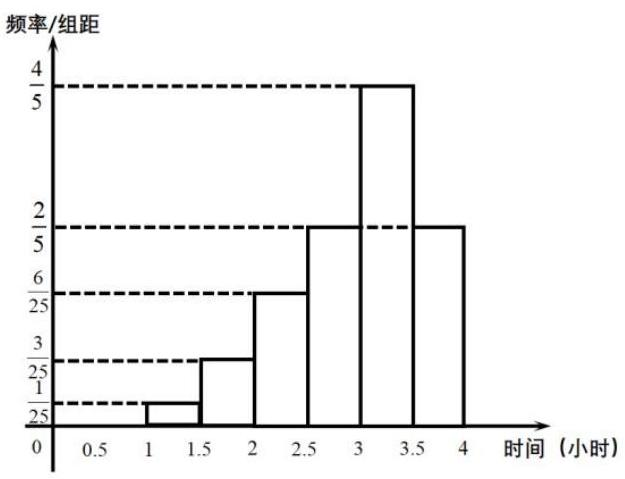
\includegraphics[max width=0.5\textwidth]{images/bo_d7fhnv491nqc73ercsbg_200_257_194_625_479_0.jpg}
\end{center}
\hspace*{3em} 

(1)试估计该校高三学生周末线上学习时间的平均数 \(\overline{x}\) 及中位数 \({x}_{0}\) (注:为了计算均值， 可用区间的中点值给区间内的每个数据赋值);

(2)现从全部高三年级学生中随机抽取 \(n\) 人，若其中有 4 人周末线上学习的时间不小于 3 小时的可能性最大,求 \(n\) 的值.

【答案】(1) \(\bar{x} = 3,{x}_{0} = {3.125};\left( 2\right) n = 6\)

【解析】(1) \(\bar{x} = \left( {{1.25} \times  \frac{1}{25} + {1.75} \times  \frac{3}{25} + {2.25} \times  \frac{6}{25} + {2.75} \times  \frac{2}{5} +  + {3.25} \times  \frac{4}{5} + {3.75} \times  \frac{2}{5}}\right)  \times  {0.5} = \therefore \; {0.4} + \left( {{x}_{0} - 3}\right)  \times  \frac{4}{5} = {0.5}\) ,解得 \({x}_{0} = {3.125}\) . ...6 分

(2)样本中线上学习时间不少于 3 小时频率为 \(\left( {\frac{4}{5} + \frac{2}{5}}\right)  \times  \frac{1}{2} = \frac{3}{5}\) ，以样本估计总体，线上学习时间不少于 3 小时的概率 \(\frac{3}{5}\) . 记 \(X\) 为从 \(n\) 人中抽取的线上学习时间不少于 3 小时的人数, 则

\[
P\left( {n,k}\right)  = {C}_{n}^{k}{\left( \frac{3}{5}\right) }^{k}{\left( \frac{2}{5}\right) }^{n - k}(n,k \in  N,n \geq  4,k = 0,1,2,\cdots \cdots
\]

2 分

由 \(\left\{  \begin{array}{l} {C}_{n}^{k}{\left( \frac{3}{5}\right) }^{k}{\left( \frac{2}{5}\right) }^{n - k} \geq  {C}_{n}^{k + 1}{\left( \frac{3}{5}\right) }^{k + 1}{\left( \frac{2}{5}\right) }^{n - k - 1} \\  {C}_{n}^{k}{\left( \frac{3}{5}\right) }^{k}{\left( \frac{2}{5}\right) }^{n - k} \geq  {C}_{n}^{k - 1}{\left( \frac{3}{5}\right) }^{k - 1}{\left( \frac{2}{5}\right) }^{n - k + 1} \end{array}\right.\) , .2 分

解得 \(\frac{{3n} - 2}{5} \leq  k \leq  \frac{{3n} + 3}{5}\) , ...2 分

由题意 \(\frac{{3n} - 2}{5} \leq  4 \leq  \frac{{3n} + 3}{5}\) ,解得 \(\frac{17}{3} \leq  n \leq  \frac{22}{3}\) ,因为 \(n \geq  4\) ,所以 \(n = 6\) 或 \(n = 7\) .

所以,当 \(n = 6\) 或 \(n = 7\) 时,其中有 4 人周末线上学习的时间不小于 3 小时的可能性最大.

...2 分

第 31页(共 35页)

7. (2025 高三二模金山 19)为了研究高三学生每天整理数学错题的情况，某校数学建模兴趣小组的同学在本校高三年级学生中采用随机抽样的方法抽取了 40 名学生，调查他们平时的数学成绩和整理数学错题的情况, 现统计得部分数据如下:

\begin{center}
\adjustbox{max width=\textwidth}{
\begin{tabular}{|c|c|c|c|}
\hline
\phantom{X} & 数学成绩总评优秀人数 & 数学成绩总评非优秀人数 & 合计 \\
\cline{1-4}
每天都整理数学错题人数 & 14 & \phantom{X} & \phantom{X} \\
\cline{1-4}
不是每天都整理数学错题人数 & \phantom{X} & 15 & 20 \\
\cline{1-4}
合计 & \phantom{X} & \phantom{X} & 40 \\
\cline{1-4}
\hline
\end{tabular}
}
\end{center}

(1)完成上述样本数据的 2×2 列联表，并计算:每天都整理数学错题且数学成绩总评优秀的经验概率;

(2)是否有 99\% 的把握认为“数学成绩总评优秀与每天都整理数学错题有关”？

\begin{center}
\adjustbox{max width=\textwidth}{
\begin{tabular}{|c|c|c|c|}
\hline
\(\alpha\) & 0.10 & 0.01 & 0.001 \\
\cline{1-4}
\(P\left( {{\chi }^{2} \geq  \alpha }\right)\) & 2.706 & 6.635 & 10.828 \\
\cline{1-4}
\hline
\end{tabular}
}
\end{center}

附:

\({\chi }^{2} = \frac{n{\left( ad - bc\right) }^{2}}{\left( {a + b}\right) \left( {c + d}\right) \left( {a + c}\right) \left( {b + d}\right) };\)

(3)从不是每天都整理数学错题的学生中随机抽取 3 名学生做进一步访谈，设恰好抽取到数学成绩总评优秀的人数为 \(X\) ,求 \(X\) 的分布和期望.

【答案】(1)2×2 列联表见解析，每天都整理数学错题且数学成绩总评优秀的经验概率为 0.35 ; (2)有 99\%的把握认为数学成绩总评优秀与每天都整理数学错题有关；(3) \(X\) 的分布为: \(\left( \begin{matrix} 0 & 1 & 2 & 3 \\  \frac{91}{228} & \frac{35}{76} & \frac{5}{38} & \frac{1}{114} \end{matrix}\right) ,E\left\lbrack  X\right\rbrack   = \frac{3}{4}\)

【解析】(1)填表如下 ......2 分

\begin{center}
\adjustbox{max width=\textwidth}{
\begin{tabular}{|c|c|c|c|}
\hline
\phantom{X} & 数学成绩总评优秀人数 & 数学成绩总评非优秀人数 & 合计 \\
\cline{1-4}
每天都整理数学错题人数 & 14 & 6 & 20 \\
\cline{1-4}
不是每天都整理数学错题人数 & 5 & 15 & 20 \\
\cline{1-4}
合计 & 19 & 21 & 40 \\
\cline{1-4}
\hline
\end{tabular}
}
\end{center}

每天都整理数学错题且数学成绩总评优秀的经验概率 \(\widehat{P} = \frac{14}{40} = {0.35}\) .

(2)提出原假设 \({H}_{0}\) :数学成绩总评优秀与每天都整理数学错题无关. .5 分确定显著性水平 \(\alpha  = {0.01}\) ,即 \(P\left( {{\chi }^{2} \geq  {6.635}}\right)  \approx  {0.01}\)

计算 \({\chi }^{2} = \frac{{40} \times  {\left( {14} \times  {15} - 6 \times  5\right) }^{2}}{{20} \times  {20} \times  {19} \times  {21}} \approx  {8.120} > {6.635}\) , .7 分

所以原假设 \({H}_{0}\) 不成立，即有 99\% 的把握认为数学成绩总评优秀与每天都整理数学错题有关. 8 分

(3)不是每天都整理数学错题的学生中数学成绩总评优秀的有 5 个，不优秀的有 15 个，恰好抽取到数学成绩总评优秀的人数为 \(X\) ,

\(P\left( {X = 0}\right)  = \frac{{\mathrm{C}}_{5}^{0}{\mathrm{C}}_{15}^{3}}{{\mathrm{C}}_{20}^{3}} = \frac{91}{228},P\left( {X = 1}\right)  = \frac{{\mathrm{C}}_{5}^{1}{\mathrm{C}}_{15}^{2}}{{\mathrm{C}}_{20}^{3}} = \frac{35}{76},\)

\(P\left( {X = 2}\right)  = \frac{{\mathrm{C}}_{5}^{2}{\mathrm{C}}_{15}^{1}}{{\mathrm{C}}_{20}^{3}} = \frac{5}{38},P\left( {X = 3}\right)  = \frac{{\mathrm{C}}_{5}^{3}{\mathrm{C}}_{15}^{0}}{{\mathrm{C}}_{20}^{3}} = \frac{1}{114},\) 12 分

故 \(X\) 的分布为: \(\left( \begin{matrix} 0 & 1 & 2 & 3 \\  \frac{91}{228} & \frac{35}{76} & \frac{5}{38} & \frac{1}{114} \end{matrix}\right)\) 13 分

所以 \(X\) 的期望为 \(E\left( X\right)  = 0 \times  \frac{91}{228} + 1 \times  \frac{35}{76} + 2 \times  \frac{5}{38} + 3 \times  \frac{1}{114} = \frac{3}{4}\) . 14 分

8. (2025 高三二模嘉定 19)某学校对学生的课外阅读时间进行调查，随机抽取了 150 位学生, 得到如下样本数据频率分布直方图.

\begin{center}
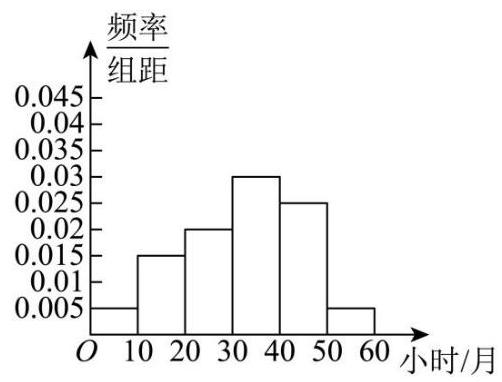
\includegraphics[max width=0.4\textwidth]{images/bo_d7fhnv491nqc73ercsbg_202_238_1175_502_382_0.jpg}
\end{center}
\hspace*{3em} 

(1)估计该校学生的平均课外阅读时间；(同一组数据用该区间的中点值作代表)

(2)估计该校学生课外阅读时间位于区间 \(\lbrack {30},{60})\) (单位:小时/月)的概率；

(3)已知该校喜欢阅读的学生占比为 18\%，初一年级学生占该校总学生数的 28\%，且初一年级学生中喜欢阅读的占 40\%，求其他年级学生中喜欢阅读的比例. (精确到 0.1\%)

【答案】(1)平均课外阅读时间32 小时/月；(2) 0.6；(3) 9.4\%.

【解析】(1) 由直方图知, 平均课外阅读时间为

\({0.05} \times  5 + {0.15} \times  {15} + {0.2} \times  {25} + {0.3} \times  {35} + {0.25} \times  {45} + {0.05} \times  {55} = {32}\) 小时/月.

(2)由直方图知,时间位于区间 \(\lbrack {30},{60})\) 的频率为 \(\left( {{0.03} + {0.025} + {0.005}}\right)  \times  {10} = {0.6}\) ， 所以该校学生课外阅读时间位于区间 \(\lbrack {30},{60})\) (单位:小时/月)的概率为 0.6 .

(3)由题设，初一年级学生中喜欢阅读的学生占比为 \({28}\%  \times  {40}\%  = {11.2}\%\) ，

所以其他年级学生中喜欢阅读的学生占比为 \({18}\%  - {11.2}\%  = {6.8}\%\) ,

故其他年级学生中喜欢阅读的比例 \(\frac{{6.8}\% }{1 - {28}\% } \approx  {9.4}\%\) .

9. (2025 高三二模崇明 19)某区 2025 年 3 月 31 日至 4 月 13 日的天气预报如图所示.

\begin{center}
\adjustbox{max width=\textwidth}{
\begin{tabular}{|c|c|c|c|c|c|c|}
\hline
\makecell{ 31 \\ 
\includegraphics[max width=0.2\textwidth]{images/bo_d7fhnv491nqc73ercsbg_203_305_621_67_62_0.jpg} \\ 大部分晴 17/9 \textdegree C } & \makecell{ 04月01日 \\ 
\includegraphics[max width=0.2\textwidth]{images/bo_d7fhnv491nqc73ercsbg_203_470_623_69_59_0.jpg} \\ 阵雨 18/9 \textdegree C } & \makecell{ 02 \\ 
\includegraphics[max width=0.2\textwidth]{images/bo_d7fhnv491nqc73ercsbg_203_637_621_68_61_0.jpg} \\ 阵雨 18/10 \textdegree C } & \makecell{ 03 \\ 
\includegraphics[max width=0.2\textwidth]{images/bo_d7fhnv491nqc73ercsbg_203_805_621_66_61_0.jpg} \\ 阵雨 19/10 \textdegree C } & \makecell{ 04 \\ 
\includegraphics[max width=0.2\textwidth]{images/bo_d7fhnv491nqc73ercsbg_203_973_621_65_63_0.jpg} \\ 多云 18/9 \textdegree C } & \makecell{ 05 \\ 
\includegraphics[max width=0.2\textwidth]{images/bo_d7fhnv491nqc73ercsbg_203_1141_622_64_61_0.jpg} \\ 间歇性多云 19/10 \textdegree C } & \makecell{ 06 \\ 
\includegraphics[max width=0.2\textwidth]{images/bo_d7fhnv491nqc73ercsbg_203_1306_621_67_63_0.jpg} \\ 多云 20/10 \textdegree C } \\
\cline{1-7}
\makecell{ 07 \\ 
\includegraphics[max width=0.2\textwidth]{images/bo_d7fhnv491nqc73ercsbg_203_304_834_67_61_0.jpg} \\ 阵雨 19/10 \textdegree C } & \makecell{ 08 \\ 
\includegraphics[max width=0.2\textwidth]{images/bo_d7fhnv491nqc73ercsbg_203_470_835_68_63_0.jpg} \\ 大部分多云 19/10 \textdegree C } & \makecell{ 09 \\ 
\includegraphics[max width=0.2\textwidth]{images/bo_d7fhnv491nqc73ercsbg_203_639_835_66_61_0.jpg} \\ 大部分晴 20/8 \textdegree C } & \makecell{ 10 \\ 
\includegraphics[max width=0.2\textwidth]{images/bo_d7fhnv491nqc73ercsbg_203_806_835_65_62_0.jpg} \\ 多云 18/8 \textdegree C } & \makecell{ 11 \\ 
\includegraphics[max width=0.2\textwidth]{images/bo_d7fhnv491nqc73ercsbg_203_973_835_65_61_0.jpg} \\ 大部分晴 18/10 \textdegree C } & \makecell{ 12 \\ 
\includegraphics[max width=0.2\textwidth]{images/bo_d7fhnv491nqc73ercsbg_203_1140_834_65_61_0.jpg} \\ 阵雨 17/8 \textdegree C } & \makecell{ 13 \\ 
\includegraphics[max width=0.2\textwidth]{images/bo_d7fhnv491nqc73ercsbg_203_1306_834_66_61_0.jpg} \\ 阵雨 17/9 \textdegree C } \\
\cline{1-7}
\hline
\end{tabular}
}
\end{center}

(1)从 3 月 31 日至 4 月 13 日某天开始，连续统计三天，求这三天中至少有两天是阵雨的概率;

(2)根据天气预报，该区 4 月 14 日的最低气温是 \({9}^{ \circ  }\mathrm{C}\) ，温差是指一段时间内最高温度与最低温度之间的差值,例如 3 月 31 日的最高温度为 \({17}^{ \circ  }\mathrm{C}\) ,最低温度为 \({9}^{ \circ  }\mathrm{C}\) ,当天的温差为 \({8}^{ \circ  }\mathrm{C}\) . 记 4 月 1 日至 4 日这 4 天温差的方差为 \({s}_{1}^{2}\) ,4 月 11 日至 14 日这 4 天温差的方差为 \({s}_{2}^{2}\) ,若 \({s}_{2}^{2} = \frac{4}{3}{s}_{1}^{2}\) ,求 4 月 14 日天气预报的最高气温;

(3)从3月31日至4月13日中随机抽取两天，用 \(X\) 表示一天温差不高于 \({9}^{ \circ  }\mathrm{C}\) 的天数，求 \(X\) 的分布列及期望.

【答案】(1) \(\frac{1}{3}\) ；(2) \({18}^{ \circ  }\mathrm{C}\) ；(3) \(X\) 的分布列为 \(\left( \begin{matrix} 0 & 1 & 2 \\  \frac{3}{91} & \frac{33}{91} & \frac{55}{91} \end{matrix}\right) ,E\left\lbrack  X\right\rbrack   = \frac{11}{7}\) .

【解析】(1) 设“从 3 月 31 日至 4 月 13 日某天开始，连续统计三天，这三天中至少有两天是阵雨”为事件 \(\mathrm{A}\) ,连续统计三天共有 12 个样本点,事件 \(\mathrm{A}\) 共有 4 个样本点,所以 \(P\left( A\right)  = \frac{4}{12} = \frac{1}{3}.\) .4 分

(2)4 月 1 日至 4 日这 4 天温差分别为 \({9}^{ \circ  }\mathrm{C}\text{ 、 }{8}^{ \circ  }\mathrm{C}\text{ 、 }{9}^{ \circ  }\mathrm{C}\text{ 、 }{9}^{ \circ  }\mathrm{C}\) ,

因此 \({s}_{1}^{2} = \frac{1}{4}\mathop{\sum }\limits_{{i = 1}}^{4}{\left( {x}_{i} - \bar{x}\right) }^{2} = \frac{3}{16}\) ,设 4 月 14 日的温差为 \({x}^{ \circ  }\mathrm{C}\) ,

则 4 月 11 日至 14 日这 4 天温差分别为 \({8}^{ \circ  }\mathrm{C}\text{ 、 }{9}^{ \circ  }\mathrm{C}\text{ 、 }{8}^{ \circ  }\mathrm{C}\text{ 、 }{x}^{ \circ  }\mathrm{C}\) ,

因此 \(\bar{x} = \frac{x + {25}}{4}{}^{ \circ  }C\) , \({s}_{2}^{2} = \frac{1}{4}\left\lbrack  {{\left( 8 - \frac{x + {25}}{4}\right) }^{2} \times  2 + {\left( 9 - \frac{x + {25}}{4}\right) }^{2} + {\left( x - \frac{x + {25}}{4}\right) }^{2}}\right\rbrack   = \frac{4}{3} \times  \frac{3}{16},\)

解得 \(x = 9\) ,因此,4 月 11 日这天最高气温是 \({18}^{ \circ  }\mathrm{C}\) .4 分

(3)从 3 月 31 日至 4 月 13 日，一天温差不超过 \({9}^{ \circ  }\mathrm{C}\) 的共有 11 天，

随机变量 \(X\) 的分布列是 \(\left( \begin{matrix} 0 & 1 & 2 \\  \frac{3}{91} & \frac{33}{91} & \frac{55}{91} \end{matrix}\right)\) ,

随机变量 \(X\) 的期望 \(E\left\lbrack  X\right\rbrack   = 0 \times  \frac{3}{91} + 1 \times  \frac{33}{91} + 2 \times  \frac{55}{91} = \frac{11}{7}\) .6 分
\end{document}